\documentclass[12pt]{report}


% Macro definitions, packages
% linking and coloring
\usepackage{color}   %May be necessary if you want to color links
\usepackage[hidelinks]{hyperref}
\hypersetup{
    colorlinks=false, %set true if you want colored links
    linktoc=all,     %set to all if you want both sections and subsections linked
    linkcolor=blue,  %choose some color if you want links to stand out
}
% \usepackage[hidelinks]{hyperref}


% \usepackage[margin=1in]{geometry}


% List of appendix and centering
\usepackage{tocloft}
\newcommand{\listappendicesname}{\begin{centering}~~~~~~~~~~~~List of Appendices\end{centering}}
\newlistof{appendices}{apc}{\listappendicesname}
\newcommand{\appendices}[1]{\addcontentsline{apc}{appendices}{\thechapter~#1}}
\newcommand{\newappendix}[1]{\chapter{#1}\appendices{#1}}
\renewcommand{\cfttoctitlefont}{\hspace*{\fill}\Huge\bfseries}
\renewcommand{\cftaftertoctitle}{\hspace*{\fill}}
\renewcommand{\cftlottitlefont}{\hspace*{\fill}\Huge\bfseries}
\renewcommand{\cftafterlottitle}{\hspace*{\fill}}
\renewcommand{\cftloftitlefont}{\hspace*{\fill}\Huge\bfseries}
\renewcommand{\cftafterloftitle}{\hspace*{\fill}}

\newcommand{\threestars}{\begin{center}$ {\bullet}\,{\bullet}\,{\bullet} $\end{center}}


\usepackage{setspace}
\usepackage{upgreek}
\usepackage{url}
\usepackage{booktabs}
\usepackage{upgreek}
\usepackage{graphicx}
\usepackage{color}
\usepackage{amsmath}
\usepackage{amssymb}
\usepackage{slashed}
\usepackage{mathalfa}
\usepackage{float}
\usepackage{overpic}
\usepackage{afterpage}
\usepackage{pdfpages}


% \usepackage{natbib}
% \usepackage{unsrt}

\usepackage[section]{placeins}



\usepackage{physics}
\usepackage{braket} % include after physics
\usepackage{xspace}

\usepackage{multirow}
\usepackage{indentfirst}

\usepackage[margin=1.5cm]{caption}
\usepackage{subcaption}
% \usepackage[splitrule]{footmisc}
\interfootnotelinepenalty=10000



\def\code#1{\texttt{#1}}

\usepackage{dcolumn}
\newcolumntype{d}[1]{D{.}{.}{#1} }
\newcolumntype{C}[1]{>{\centering\arraybackslash}m{#1}}
\usepackage{makecell}




% feynman diagrams
\usepackage{tikz-feynman}
\tikzfeynmanset{compat=1.0.0}
\usepackage{rotating}


\newcommand*{\titleName}{Searches for the Rare Decay of the Higgs Boson to Two Muons and for New Physics in Dilepton Final States with the ATLAS Experiment}

% particles
\newcommand*{\pp}{\ensuremath{pp}\xspace}
\newcommand*{\mm}{\ensuremath{\mu\mu}\xspace}
\newcommand*{\tautau}{\ensuremath{\tau\tau}\xspace}
\newcommand*{\ee}{\ensuremath{ee}\xspace}
\let\llt\ll % booya!
\renewcommand*{\ll}{\ensuremath{\ell\ell}\xspace}
\newcommand*{\W}{\ensuremath{W^\pm}\xspace}
\newcommand*{\Wp}{\ensuremath{W^+}\xspace}
\newcommand*{\Wm}{\ensuremath{W^-}\xspace}
\newcommand*{\Z}{\ensuremath{Z}\xspace}
\newcommand*{\jpsi}{\ensuremath{J/\psi}\xspace}
\newcommand*{\vhmm}{\ensuremath{V(H\to\mu\mu)}\xspace}
\newcommand*{\vhllmm}{\ensuremath{VH\to\ell(\ell/\nu)\mu\mu}\xspace}
\newcommand*{\mh}{\ensuremath{m_{\text{H}}}\xspace}
\newcommand*{\muu}{\ensuremath{m_{\mu\mu}}\xspace}
\newcommand*{\mee}{\ensuremath{m_{ee}}\xspace}
\newcommand*{\mll}{\ensuremath{m_{\ell\ell}}\xspace}
\newcommand*{\qqll}{\ensuremath{q\overline{q}\ell^+\ell^-}\xspace}
\newcommand*{\llqq}{\ensuremath{\qqll}\xspace}
\newcommand*{\e}{\ensuremath{e}\xspace}
\newcommand*{\m}{\ensuremath{\mu}\xspace}
\newcommand*{\h}{\ensuremath{H}\xspace}
\newcommand*{\pt}{\ensuremath{p_\text{T}}\xspace}
\newcommand*{\vecpt}{\ensuremath{\vec{p}_\text{T}}\xspace}
\newcommand*{\plong}{\ensuremath{p_\text{L}}\xspace}
\newcommand*{\httt}{\ensuremath{H_\text{T}}\xspace}
\newcommand*{\mt}{\ensuremath{E_\text{T}}\xspace}
\newcommand*{\et}{\ensuremath{E_\text{T}}\xspace}
\newcommand*{\met}{\ensuremath{E_T^\mathrm{miss}}\xspace}
\newcommand*{\sqrts}{\ensuremath{\sqrt{s}}\xspace}
\newcommand*{\sqrths}{\ensuremath{\sqrt{\hat{s}}}\xspace}

\newcommand*{\zhat}{\ensuremath{\hat{z}}\xspace}
\newcommand*{\xhat}{\ensuremath{\hat{x}}\xspace}
\newcommand*{\yhat}{\ensuremath{\hat{y}}\xspace}

% chiralities
\newcommand*{\fl}{\ensuremath{f_\text{L}}\xspace}
\newcommand*{\fr}{\ensuremath{f_\text{R}}\xspace}
\newcommand*{\flp}{\ensuremath{f'_\text{L}}\xspace}
\newcommand*{\frp}{\ensuremath{f'_\text{R}}\xspace}
\newcommand*{\ufl}{\ensuremath{\overline{f}_\text{L}}\xspace}
\newcommand*{\ufr}{\ensuremath{\overline{f}_\text{R}}\xspace}
\newcommand*{\uflp}{\ensuremath{\overline{f}'_\text{L}}\xspace}
\newcommand*{\ufrp}{\ensuremath{\overline{f}'_\text{R}}\xspace}

% mandelstram
\newcommand*{\shat}{\ensuremath{\hat{s}}\xspace}
\newcommand*{\uhat}{\ensuremath{\hat{u}}\xspace}
\newcommand*{\that}{\ensuremath{\hat{t}}\xspace}
\newcommand*{\qbar}{\ensuremath{\overline{q}}\xspace}
\newcommand*{\ubar}{\ensuremath{\overline{u}}\xspace}
\newcommand*{\dbar}{\ensuremath{\overline{d}}\xspace}
\newcommand*{\pbar}{\ensuremath{\overline{p}}\xspace}
\newcommand*{\fbar}{\ensuremath{\overline{f}}\xspace}
\newcommand*{\tbar}{\ensuremath{\overline{t}}\xspace}
\newcommand*{\bbar}{\ensuremath{\overline{b}}\xspace}
\newcommand*{\cbar}{\ensuremath{\overline{c}}\xspace}
\newcommand*{\ttbar}{\ensuremath{t\overline{t}}\xspace}
\newcommand*{\bbbar}{\ensuremath{b\overline{b}}\xspace}

\newcommand*{\neutralcone}{\ensuremath{\pt^\text{neu20}}\xspace}
\newcommand*{\ptconeThirty}{\ensuremath{\pt^\text{cone30}}\xspace}
\newcommand*{\ptcone}{\ensuremath{\pt^\text{cone20}}\xspace}
\newcommand*{\ptvarconeMuon}{\ensuremath{\pt^\text{varcone30}}\xspace}
\newcommand*{\ptvarconeElec}{\ensuremath{\pt^\text{varcone20}}\xspace}
\newcommand*{\etcone}{\ensuremath{\et^\text{topocone20}}\xspace}
\newcommand*{\xsbr}{\ensuremath{\sigma_\text{visible}\times\text{BR}}\xspace}
\newcommand*{\acceff}{\ensuremath{\mathcal{A}\times\epsilon_\text{sig}}\xspace}
\newcommand*{\lam}{\ensuremath{\Lambda}\xspace}
\newcommand*{\nsig}{\ensuremath{N_\text{sig}}\xspace}
\newcommand*{\nbkg}{\ensuremath{N_\text{bkg}}\xspace}

% Generators
\newcommand*{\powheg}{\textsc{Powheg-Box}\xspace}
\newcommand*{\sherpa}{\textsc{Sherpa}\xspace}
\newcommand*{\madgraph}{\textsc{MadGraph5}\_aMC@NLO\xspace}
\newcommand*{\pythia}{\textsc{Pythia}\xspace}
\newcommand*{\evtgen}{\textsc{EvtGen}\xspace}
\newcommand*{\geant}{\textsc{Geant4}\xspace}
\newcommand*{\xgb}{\code{XGBoost}\xspace}
\newcommand*{\etal}{\emph{et~al.}\xspace}




% statistics
\newcommand*{\cls}{\ensuremath{\text{CL}_\text{s}}\xspace}
\newcommand*{\clb}{\ensuremath{\text{CL}_\text{b}}\xspace}
\newcommand*{\clsb}{\ensuremath{\text{CL}_\text{s+b}}\xspace}
\newcommand*{\mus}{\ensuremath{\mu_\text{S}}\xspace}
\newcommand*{\nss}{\ensuremath{N_\text{ss}}\xspace}

% processes
\newcommand*{\hmm}{\ensuremath{H\to\mm}\xspace}
\newcommand*{\nr}{\ensuremath{non-resonant}\xspace}

% units
\newcommand*{\cms}{\ensuremath{\text{cm}^{-2}\text{s}^{-1}}\xspace}
\newcommand*{\fb}{\ensuremath{\text{fb}^{-1}}\xspace}
\newcommand*{\um}{\ensuremath{\mu\text{m}}\xspace}
\newcommand*{\us}{\ensuremath{\mu\text{s}}\xspace}

% variables

\newcommand*{\half}{\ensuremath{\frac{1}{2}}\xspace}
\newcommand*{\as}{\ensuremath{\alpha_s\xspace}}
\newcommand*{\reals}{\ensuremath{\mathbb{R}}\xspace}
\newcommand*{\ident}{\ensuremath{\mathbb{I}}\xspace}
\newcommand*{\nxn}{\ensuremath{n\times n}\xspace}

\newcommand*{\vtheta}{\ensuremath{\vec{\theta}}\xspace}
\newcommand*{\poincare}{Poincar\'e\xspace}
\renewcommand*{\check}{{\color{red}[check]}\xspace}


\usepackage[utf8]{inputenc}
\usepackage[T1]{fontenc}
\usepackage{lmodern}
% \usepackage[showframe, textwidth = 15cm, nomarginpar, noheadfoot]{geometry}
\usepackage{mathtools}
\newcommand{\shortnote}[1]{ &  & \text{\smal4l\llap{#1}}}
\newcommand{\longeqnote}[1]{& & \\ \notag  &  &  &  &  & \text{\small\llap{#1}}}

\newcommand{\centered}[1]{\begin{tabular}{l} #1 \end{tabular}}

% statistics
\newcommand*{\nobs}{\ensuremath{N_\mathrm{text}}\xspace}


\newcommand*{\POWHEG}{\textsc{Powheg}\xspace}
\newcommand*{\POWHEGV}[1]{\textsc{Powheg}~#1\xspace}
\newcommand*{\POWHEGBOX}{\textsc{Powheg-Box}\xspace}
\newcommand*{\POWHEGBOXV}[1]{\textsc{Powheg-Box}~#1\xspace}
\newcommand*{\PYTHIA}{\textsc{Pythia}\xspace}
\newcommand*{\PYTHIAV}[1]{\textsc{Pythia}~#1\xspace}
\newcommand*{\SHERPA}{\textsc{Sherpa}\xspace}
\newcommand*{\SHERPAV}[1]{\textsc{Sherpa}~#1\xspace}
\newcommand*{\GEANT}{\textsc{Geant}\xspace}



% ############################################################
% Commands for Ensemble Appendix
% ############################################################
\newcommand*{\spur}{\ensuremath{\sigma^\mathrm{spur}}\xspace}
\newcommand*{\func}{\ensuremath{f(\mll)}\xspace}
\newcommand*{\truth}{\ensuremath{f^\mathrm{truth}(\mll)}\xspace}
\newcommand*{\realsBkg}{\ensuremath{\mathbb{R}^{\dbkg}}\xspace}
\newcommand*{\realsSyst}{\ensuremath{\mathbb{R}^{\dsyst}}\xspace}
\newcommand*{\eeReal}{\ensuremath{\mathbb{R}}\xspace}
\newcommand*{\map}{\ensuremath{h(\realsBkg)\mapsto\eeReal}\xspace}
% mapping theta->bkg shape
\newcommand*{\mapThetaToBkg}{\ensuremath{g(\nps|\systs)\mapsto\realsBkg}\xspace}
\newcommand*{\thetaToBkg}{\ensuremath{g(\nps|\systs)}\xspace}
\newcommand*{\eeDd}{\ensuremath{\Delta}\xspace}
\newcommand*{\deltaTheta}{\ensuremath{\Delta^\theta}\xspace}
\newcommand*{\deltaD}{\ensuremath{\Delta^D}\xspace}
\newcommand*{\deltaDSquared}{\ensuremath{(\Delta^D)^2}\xspace}
\newcommand*{\deltaThetaSquared}{\ensuremath{(\Delta^\theta)^2}\xspace}
\newcommand*{\np}{\ensuremath{\theta_i}\xspace}
\newcommand*{\npmeasured}{\ensuremath{\hat{\theta_i}}\xspace}
\newcommand*{\npprob}{\ensuremath{G(\theta_i)}\xspace}
\newcommand*{\nps}{\ensuremath{\vec{\theta}}\xspace}
% Dimensions
\newcommand*{\ddata}{\ensuremath{N_\mathrm{data}}\xspace}
\newcommand*{\dbkg}{\ensuremath{N_\mathrm{bkg}}\xspace}
\newcommand*{\dsyst}{\ensuremath{N_\mathrm{syst}}\xspace}
% mean and std
\newcommand*{\meanD}{\ensuremath{\mathrm{E}[\deltaD]}\xspace}
\newcommand*{\meanDSquared}{\ensuremath{\mathrm{E}[(\deltaD)^2]}\xspace}
\newcommand*{\meanTheta}{\ensuremath{\mathrm{E}[\deltaTheta]}\xspace}
\newcommand*{\meanThetaSquared}{\ensuremath{\mathrm{E}[(\deltaTheta)^2]}\xspace}
\newcommand*{\stdD}{\ensuremath{\mathrm{var}[\deltaD]}\xspace}
\newcommand*{\stdTheta}{\ensuremath{\mathrm{var}[\deltaTheta]}\xspace}
% # datasets
\newcommand*{\template}{\ensuremath{\vec{D}}\xspace}
\newcommand*{\mc}{\ensuremath{\vec{D}^\mathrm{MC}}\xspace}
\newcommand*{\data}{\ensuremath{\vec{D}^\mathrm{data}}\xspace}
\newcommand*{\truthdata}{\ensuremath{\vec{D}^\mathrm{truth}}\xspace}
\newcommand*{\truthguess}{\ensuremath{\vec{X}^\mathrm{truth}}\xspace}
\newcommand*{\syst}{\ensuremath{\vec{D}^\mathrm{syst}_i}\xspace}
\newcommand*{\systUp}{\ensuremath{\vec{D}^\mathrm{+syst}_i}\xspace}
\newcommand*{\systDn}{\ensuremath{\vec{D}^\mathrm{-syst}_i}\xspace}
\newcommand*{\systs}{\ensuremath{\{\vec{D}^\mathrm{syst}\}}\xspace}
% analysis functions
\newcommand*{\eeNbkg}{\ensuremath{F(\vec{D})}\xspace}
\newcommand*{\nbkgmc}{\ensuremath{F(\mc)}\xspace}
\newcommand*{\nbkgdata}{\ensuremath{F(\data)}\xspace}
\newcommand*{\nbkgtruth}{\ensuremath{F(\truthdata)}\xspace}

\newcommand*{\gsm}{\ensuremath{\text{G}_\text{SM}}\xspace}

\newcommand*{\feynx}{\ensuremath{x}\xspace}

\newcommand*{\first}{1\textsuperscript{st}\xspace}
\newcommand*{\second}{2\textsuperscript{nd}\xspace}
\newcommand*{\third}{3\textsuperscript{rd}\xspace}


% Bib info
\usepackage{cite}
% \addbibresource{resources.bib}
% \usepackage[margin=0.7in]{geometry} % 1in for Umich
\usepackage[margin=1.0in]{geometry} % 1in for Umich
\setcounter{errorcontextlines}{50}

\title{\titleName}
\author{Aaron White}

% \setstretch{0.9} % 1.5 for Umich
\onehalfspacing



\begin{document}

\pagenumbering{gobble}
\begin{titlepage}

\begin{center}
\phantom{x}\\
\vspace{10em}
\textbf{\Large\titleName}\\
\vspace{5em}
by\\
Aaron White\\
\vspace{5em}
{\singlespacing
A dissertation submitted in partial fulfillment\\
of the requirements for the degree of\\
Doctor of Philosophy\\
(Physics)\\
in The University of Michigan\\
2021\\
}
\end{center} 

\vspace{5em}
{\singlespacing
\noindent Doctoral Comittee:\\
\phantom{xxxx} Professor Bing Zhou, Chair \\
\phantom{xxxx} Professor Christine Aidala\\
\phantom{xxxx} Professor David Baker\\
\phantom{xxxx} Professor Tom Schwarz\\
\phantom{xxxx} Professor James Wells\\
}

\end{titlepage}

\clearpage

\begin{center}
\doublespacing
\vspace*{\fill}
\href{http://hg8i.com/thesis/}{Aaron White} \\
aaronsw@umich.edu \\
ORCID iD: 0000-0003-0714-1466 \\
\vspace{3em}
\textcopyright Aaron White 2021
\vspace*{\fill}
\end{center}

\thispagestyle{empty}


\pagenumbering{roman}
\cleardoublepage
\phantomsection
\addcontentsline{toc}{chapter}{Dedication}
\phantom{x}\\
\phantom{x}\\
\vspace{1.1em}

\begin{center}
\textbf{\LARGE Dedication}
\end{center}

% \vspace*{\fill}
\begin{center}
\emph{To my grandfather, Dr. David White}
\end{center}
% \vspace*{\fill}


\cleardoublepage
\phantomsection
\addcontentsline{toc}{chapter}{Acknowledgements}
\phantom{x}\\
\phantom{x}\\
\vspace{1.1em}

\begin{center}
\textbf{\LARGE Acknowledgements}
\end{center} 

First I would like to thank my mother, Judith White, and my siblings David White, Ben White, and Laura White, for their love and support.

I am deeply indebted to the many educators who, during the past twenty one years, have through generosity and patience exposed me to knowledge and taught me how to learn.
First I am thankful to my high school teachers John Donnelly and Eric Dennison for teaching me calculus and computer programming, and Dan Falcon, John Phipps, and Sally Hair for encouraging me to study science.
I want to thank Dartmouth College professors John Thorstensen, Robert Caldwell, and James LaBelle for introducing me to physics and astronomy.
I would also like to thank George O'Toole, Kyle Cady, and John Hammond for involving me with research during this time.

There are many University of Michigan professors that I would like to thank;
Jean Krisch for her guidance;
Dragan Huterer for teaching me introductory physics and supervising me as a freshman;
Sally Oey for teaching me stellar dynamics and supervising me in research as a sophomore;
Christine Aidala for introducing me to high energy experimental physics and supervising me in research as a junior and senior and, along with Leopoldo Pando Zayas, teaching me mathematical methods;
Michael Zieve for teaching me analysis;
Bing Zhou, Roberto Merlin, and James Liu for teaching me the most elegant of theories, electromagnetism;
Bing Zhou again, along with Aaron Leanhardt and Junjie Zhu for teaching me classical mechanics;
Jianming Qian, Tom Schwarz, and Carl Akerlof for teaching me experimental methods;
James Wells, Henriette Elvang, and Ratindranath Akhoury for teaching me quantum field theory.

I have benefited from the help and generosity of many people during my time working on this project.
I would like to thank the members the ATLAS Collaboration who have built and run the detector and computing infrastructure that has enabled my work.
Their work and mine has been supported by various national funding agencies including the Department of Energy.
I would also like to thank the engineers and staff at CERN who help operate the LHC and maintain the site and the ATLAS secretaries who have helped solve numerous problems that occur as a result of living in France.
I am thankful to the Michigan ATLAS group professors Bing Zhou, Jianming Qian, Tom Schwarz, Dan Amidei, Junjie Zhu, Jianming Qian, Homer Neal, and Jay Chapman, as well as Tiesheng Dai, for building a supportive university environment and attracting the funding that has enabled this work.
I am also thankful to faculty of the Laboratoire de l'Acc\^el\^erateur Lin\^eaire and especially Louis and Lydia Fayard.
I am thankful to the friends I have made through physics for engaging in interesting discussions, especially Tom Cheng, Yicheng Guo, Zhi Zheng, Zirui Wang, Rongkun Wang, Zhongyukun Xu, and Siyuan Sun, Yanlin Liu, Aishik Gosh, Aaron White, Ismet Siral, Corentin Allaire, Hao Liu, and Dan Marley.
In particular, Matthew Klein has provided patient and invaluable guidance on topics of data analysis.
During my authorship qualification, I benefited from the guidance of Tom Schwarz and technical instruction of Xueye Hu, Jinhong Wang, and Bob Ball.
On the search for the Higgs decay to two muons, I am thankful for the guidance of Yusheng Wu, Yanlin Liu, and Bing Li.
On the search for contact interactions, I would like to thank the Exotics-LPX Dilepton group and our ever patient editorial board, Paul de Jong, Ulla Blumenschein, and Elliot Lipelles for their feedback.
I would especially like to thank Uta Klein, Dan Hayden, Etienne Dreyer, Peter Falke, Tanya Hryn'Ova, Sean Lawler for their contributions and guidance, and Stephan Hageboeck for his statistical input.
I am thankful for the LPX and Exotics group leadership of Yasu Okumura, Nikolina Llic, Antonio Sidoti, Carl Gwilliam, and Oliver Stelzer-Chilton.
I want to remark on my great fortune to have worked on this project with Deshan Abhayasinghe and Noam Tal Hod, who have made the this project one of the highlights of the past five years.
I am thankful for the committee, Bing Zhou, Tom Schwarz, Christine Aidala, James Wells, and David Baker for reviewing this thesis.
Finally, I want to extend my deepest thanks to my advisor, Bing Zhou.
She has worked tirelessly to support me since, as an undergraduate, I enrolled in her section of Physics 405: Intermediate Electromagnetism.
As a role model, her persistent curiosity and attention to detail have provided an exceptional example to follow of an experimental physicist. 
As a mentor, she has always pushed me to work to my fullest ability.



\cleardoublepage
\phantomsection
\tableofcontents
\cleardoublepage
\phantomsection
\addcontentsline{toc}{chapter}{List of Figures}
\listoffigures
\cleardoublepage
\phantomsection
\addcontentsline{toc}{chapter}{List of Tables}
\listoftables
\cleardoublepage
\phantomsection
\addcontentsline{toc}{chapter}{List of Appendices}
\renewcommand{\thesection}{\Alph{section}}
\listofappendices
\cleardoublepage
\phantomsection
\addcontentsline{toc}{chapter}{Abstract}
\phantom{x}\\
\phantom{x}\\
\vspace{1.1em}

\begin{center}
\textbf{\LARGE Abstract}
\end{center} 

This thesis presents two topics: a search for rare dimuon decay of the Standard Model Higgs boson and a search for new physics with non-resonant phenomena at the TeV mass scale with dilepton final states.
Both studies investigate data recorded by the ATLAS experiment from $\sqrt{s}=13$~TeV proton-proton collisions produced during the second of the Large Hadron Collider at CERN.
This data corresponds to an integrated luminosity of 139~fb$^{-1}$. 
% Both studies investigate an integrated luminosity of 139~fb$^{-1}$ of data recorded by the ATLAS from $\sqrt{s}=13$~TeV proton-proton collisions from Run~2 of the Large Hadron Collider at CERN.

The first study is the search for the Standard Model Higgs boson decaying to two muons.
This decay is used to study the Higgs boson Yukawa couplings to the second generation fermions as part of a field-wide effort to study the properties of the Higgs boson.
Identifying events produced by this decay is complicated by the small Higgs boson branching fraction to muons and the large irreducible background from other Standard Model processes.
% The major Higgs production modes at the LHC are gluon-gluon fusion (ggF), vector-boson fusion (VBF), a vector boson (W or Z) associated production (VH).
Previous studies selected events using criteria that targets Higgs production through gluon-gluon fusion and vector-boson fusion mechanisms.
To increase sensitivity to Higgs produced events, new selections are added targeting vector boson associated (VH) production with a leptonic decay from the vector boson.
Multivariate analysis methods are used to identify events for different categories.
The limits set on signal production in the new phase spaces explored in this analysis are the first of their kind.
The strongest expected (observed) limit on leptonic VH production excludes signals down to 13.2 (22.6) times the Standard Model prediction.
The combination of VH with the other major production modes results in a signal significance of 2.0$\sigma$ over the background hypothesis.

The second study is a search for non-resonant phenomena in the dielectron and dimuon final states.
One possible source for this is quark and lepton compositeness at energy scales beyond direct access at the LHC.
These would lead to contact interactions that produce non-resonant enhancement in dilepton production at the TeV mass scale.
This search introduces several novel methods including a background model derived from data and a formalism to parameterization of the associated uncertainties.
% This is done in a low-mass control region where the signal is expected to be negligible, while the function is extrapolated to several high-mass signal regions where an enhancement of events is expected above the background processes.
% This approach mitigates the statistical and theoretical uncertainty of simulated background predictions.
In this search, no significant deviation in data is observed with respect to the expected background.
Upper limits on the visible cross-section times branching ratio are set in this search.
These, along with benchmark CI signal efficiencies, can be interpreted as limits in terms of a variety of signal models.
The lower limits on the energy scale of CI, $\Lambda$, reach 35.8 TeV, indicating the quarks and leptons are still point-like particles at 10$^{-20}$ m.
These are the strongest limits on \qqll contact-interactions to date.


\cleardoublepage


\pagenumbering{arabic}
% \addtocontents{toc}{%
% \protect\contentsline{part}{Chapters}{}}
% \addtocontents{toc}{\protect\contentsline{chapter}{\protect Chapters}{}{}}
\addcontentsline{toc}{part}{Chapters}

% \chapter{Introduction}

% Experimental observations are the foundations of the our knowledge of these building blocks.
% The most complete mathematical description of these building blocks based, on experimental knowledge, is the Standard Model of particle physics.


% Particles
The Universe consists of particles, the space they inhabit, and the interactions between them.
Fundamental particles are the most basic unit of matter, with observable properties including mass, charge couplings, spin, and lifetime.
Particles with integer spins are called bosons, while particles with half-integer spins are called fermions.
Particles may be composite, such as the proton, or elementary, as is assumed for the electron.
Particles and the interactions between them together form the physical world.
The most complete mathematical description of these building blocks, based on experimental knowledge, is the Standard Model (SM) of particle physics.
This theory has evolved and expanded since original development in 1974, with each iteration encompassing the consensus view of the physics community.
% The Standard model describes particles at the most fundamental, with no internal substructure.

% Added by Bing
This dissertation presents research on the nature of particle physics conducted at the Large Hadron Collider with the ATLAS experiment. 
The basic principles of particle physics are introduced in this chapter, followed by the particular research topics of this thesis.

\section{Particles, Space, and Interactions}

% Fermions
Each type of fermion exists in a pair, consisting of \emph{particles} and \emph{anti-particles} with equal mass and opposite electric charges.
The fermions are further divided into leptons with integer electric charge and quarks with fractional electric charges.
There are three \emph{flavors} of charged leptons. In ascending mass these are the electron, the muon, and the tauon.
There are also three flavors of neutral leptons, corresponding to each charged lepton flavor, called neutrinos.
Recent measurements provide an indication that the neutrino masses are ordered similarly to the order of charged leptons \cite{kamio}.
The leptons are arranged into three \emph{generations} based on the approximate conservation of the number of leptons minus the number of anti-leptons belonging to each generation in a given interaction.
There are six quarks, divided into up-type quarks and down-type quarks.
The up-type quarks are the up, charm, and top quarks.
The down-type quarks are the down, strange, and bottom quarks.
Like the leptons, up- and down-type quarks are paired together in generations of ascending mass.
Quarks commonly exist in bound-states consisting of two (meson) and three (baryon) quarks.
% Bosons
The bosons mediate forces between the particles.
The most familiar boson, the photon, mediates the electromagnetic force between charged particles.
The gluons carry the strong nuclear force, binding quarks inside multi-quark composite particles called hadrons.
The \W and \Z bosons carry the weak nuclear force, responsible for nuclear beta decays.
These bosons are called \emph{vector gauge bosons} because of their association with gauge groups.
Finally, the recently discovered scalar particle, the Higgs boson, mediates a momentum exchange between massive particles.
% Summary
These particles are summarized in Table \ref{tab:particles}.

\begin{table}[htp]
\begin{center}
\caption{Particles of the Standard Model listed along with their symbol and several properties \cite{pdg2018}. ($^*$ The graviton is not considered part of the SM.)}
{\footnotesize
\begin{tabular}{c c l c l c c c c c c}
\toprule
& & Name & Symbol & \multicolumn{1}{c}{Generation} & Charge & Spin & Mass [MeV/c$^2$] \\
\midrule
\multirow{12}{*}[0em]{\begin{sideways}Fermions\end{sideways}} & \multirow{6}{*}[0em]{\begin{sideways}Leptons\end{sideways}} & Electron & \e & ~~~~~~\first & -1 & 1/2 & 0.511 \\
& & Muon   			  & \m         & ~~~~~~\second & -1 & 1/2 & 105.7 \\
& & Tau    			  & $\tau$     & ~~~~~~\third  & -1 & 1/2 & 1776.8 \\
& & Electron Neutrino & $\nu_e$    & ~~~~~~\first  & 0  & 1/2 &  $<2\times10^{-6}$\\
& & Muon Neutrino     & $\nu_\mu$  & ~~~~~~\second & 0  & 1/2 &  $<2\times10^{-6}$\\
& & Tau Neutrino      & $\nu_\tau$ & ~~~~~~\third  & 0  & 1/2 &  $<2\times10^{-6}$\\
\cline{2-8}
& \multirow{6}{*}[0em]{\begin{sideways}Quarks\end{sideways}} & Up & $u$ & ~~~~~~\first & 2/3 & 1/2 &  $2.2\pm0.5$ \\
& & Charm             & $c$ & ~~~~~~\second &  2/3 & 1/2 &  $1.275\pm0.035\times10^{3}$ \\
& & Top               & $t$ & ~~~~~~\third  &  2/3 & 1/2 &  $173.0\pm0.4\times10^{3}$ \\
& & Down              & $d$ & ~~~~~~\first  & -1/3 & 1/2 &  $4.7\pm0.5$ \\
& & Strange           & $s$ & ~~~~~~\second & -1/3 & 1/2 &  $95\pm9$ \\
& & Bottom            & $b$ & ~~~~~~\third  & -1/3 & 1/2 &  $4.18\pm0.04\times10^{3}$ \\
\midrule
\multicolumn{2}{c}{\multirow{6}{*}[0em]{\begin{sideways}Bosons\end{sideways}}} & Photon & $\gamma$ && 0 & 1 & $<1\times10^{-24}$ \\
& & Gluon         & $g$ & & 0 & 1 & 0 \\
& & Z boson       & \Z  & & 0 & 1 & $91.1876\times 10^3$ \\
& & W boson       & \W  & & $\pm$1 & 1 & $80.39\times 10^3$ \\
& & Higgs boson   & \h  & & 0 & 0 & $125.18\times 10^3$ \\
& & Graviton$^*$  & $g$ & & 0 & 2 & $<1\times 10^{-38}$ \\
\bottomrule
\end{tabular}
}
\label{tab:particles}
\end{center}
\end{table}

While the Standard Model has been successful in the description of particles and their interactions, it is an incomplete description of the Universe.
The most visible shortcoming is the lack of a description of gravity; the quantum effects of gravity are expected to manifest themselves at energy scales that are inaccessible to modern particle experiments.
Other absences in the theory include particles that explain the phenomena of dark matter and dark energy.
The theory also lacks a single broadly accepted explanation for the mass of neutrinos, although several plausible mechanisms have been proposed \cite{jw2019}.
Ongoing experiments are investigating discrepancies between predicted and observed quantities, such as the anomalous magnetic moment of the muon.
Despite these absences the present version of the Standard Model is a remarkably predictive theory.

% \section{Spacetime}

Spacetime is the four-dimensional manifold that particles inhabit at a microscopic scale.
Three of these are spacial dimensions, and one is time: 3+1-dimensional spacetime.
The special theory of relativity describes the distinction between the dimensions: rotations from one spacial dimension to another take place in Euclidean space, while rotations from a spatial dimension into time take place in a hyperbolic space.
None of this should be taken at face value, or as posed by Ehrenfest in 1917, \emph{in what way does it become manifest in the fundamental laws of physics that space has three dimensions?}
One point to consider is the stability of elliptical orbits in a two-body system.
If the number of space dimensions exceeds three, then stable circular orbits under gravity are impossible.
This result holds for the quantum orbits of electrons around a nucleus as well.
Therefore if one is to find oneself in a universe with atoms, chemistry, and planets, then the number of spatial dimensions in which these take place is limited to three~\cite{ehrenfest}.
This limit on space dimensions suggests the question: why one time dimension?
In the case of multiple time dimensions, solutions to partial differential equations such as those that describe the laws of physics are ambiguous.
This is analogous to the situation in 3+1-dimensional spacetime wherein predictions outside the lightcone are impossible.
It has been argued by Tegmark that this precludes observers, as the lack of predictability renders reality incomprehensible~\cite{tegmark-time}.


% \section{Interactions}
Until the discovery of the Higgs boson, there were four known fundamental forces through which particles might interact: gravity, the electromagnetic force, the weak nuclear force, and the strong nuclear force.
An interaction between two or more particles entails the exchange of momentum between the participants.
For each force, the momentum exchange is mediated by a boson.
Gluons mediate the strong nuclear force.
The weak nuclear force is mediated by the \Wp, \Wm, and \Z bosons.
Photons mediate the electromagnetic force.
It is expected that gravity is mediated by a hypothetical particle called a graviton; however, this has not been observed. The gravitational interaction strength is more than an order of 40 magnitude smaller compared to the electromagnetic interaction. At the microscopic level, the interaction of the gravity could be ignored and is not included in the Standard Model.

In 2012, the ATLAS and CMS experiments at the Large Hadron Collider at CERN discovered the Higgs boson. Like the vector bosons associated with the four canonical forces, the scalar particle, Higgs boson, mediates a momentum exchange between particles. The interactions with fermions are not universal, proportional to fermion's mass.

\begin{table}[htp]
\begin{center}
\caption{Interactions in experienced by particles. The strength of the force depends on the energy scale at which it is measured, so approximate values are given \cite{robinson}. In the case of Gravity, which is not included in the Standard Model, the coupling strength is assumed to be on the order of the gravitational constant \cite{donogue}.}
{\normalsize
\begin{tabular}{c c l c c c c c c c}
\toprule
Interaction            & Force Carrier &  Relative Strength   & Range [m]  \\
\midrule
Strong           & Gluon      &  1           & $10^{-15}$ \\
Electromagnetic  & Photon     &  $10^{-2}$   & $\infty$   \\
Weak             & \W, \Z     &  $10^{-5}$   & $10^{-18}$ \\
Higgs            & Higgs      &  $<10^{-5}$  & $10^{-19}$ \\
Gravity          & Graviton   &  $ 10^{-39}$ & $\infty$   \\
\bottomrule
\end{tabular}
}
\label{tab:forces}
\end{center}
\end{table}

\section{Energies and Measures}

Enormous energy concentrations are required to enable the production of massive particles and facilitate rare interactions.
In order to study these processes, it is convenient to define units of measurements using energy as the basic unit to describe the particle mass, momentum, lifetime, and travel distance.

Energies are measured in units of \emph{electron-volts}, eV.
This is equal to the energy required to move an electron through one volt of electric potential.
One eV is a small amount of energy, equivalent the amount needed to move a single electron from one terminal of a AA battery to the other.
In the scope of discovered particles and interactions, eV are often presented along with metric prefixes.
One mega-electronvolt (MeV) is one million eV, and is the energy scale reached by the earliest circular particle accelerators with fixed magnetic fields called cyclotrons.
One giga-electronvolt (GeV) is one billion eV, and became accessible with the development of synchrotron accelerators that gradually increased their fields to reach higher energies.
One tera-electronvolt (TeV) is one trillion eV.
The stack of AA batteries required to accelerate an electron to 1 TeV would reach from Earth to Mars at its closest approach.
Although the Tevatron at Fermilab came close, the TeV scale was first reached at the Large Hadron Collider (LHC) at CERN.
The energy at the LHC subsequently accelerated protons to energies of 7~TeV.
The particular energy scales of interest in this thesis range from tens of GeV to tens of TeV.

Several quantities are useful in describing interactions between particles: energy, mass, momentum, distance, and time.
The unit of eV already describes quantities of energy.
In standard international (SI) units, energy is measured in units of joules (J) equal to kg$\frac{\text m^2}{\text s^2}$.
Mass is, therefore, expressible as energy divided by velocity squared.
A convenient velocity to use is the speed of light, $c$.
In this case, mass is expressed in units of GeV/$c^2$.
Likewise, momentum, which is measured in SI units as kg$\frac{\text m}{\text s}$, can be expressed in units of GeV/$c$.
Distance and time can be expressed with the aid of the reduced Planck's constant $\hbar=6.58\times10^{-25}~$GeV$\cdot$s.
Using $\hbar$, distance is measured in units of $\hbar c/$GeV, and time is measured in units of $\hbar/$GeV.
These are referred to as \emph{Planck units} and are commonly used throughout this thesis along with SI units following the field's standard practice.
In cases where their presence can be inferred from the quantity, the SI units are replaced such that the constants $\hbar$ and $c$ have numerical values of 1, leaving powers of GeV.
These units are summarized in Table \ref{tab:units}.

\begin{table}[htp]
\caption{Description of the units used to describe dimensions in this thesis. Each row lists equivalent quantities.}
\begin{center}
\begin{tabular}{l l l l l l}
\toprule
Dimension & SI Units &  Planck Units & Natural Units \\
          &          &               & $c=1$, $\hbar = 1$ \\
\midrule
Energy    &    1.602$\times10^{-10}$J               & ~~~~GeV            & ~~~~GeV \\
Mass      &    1.783$\times10^{-27}$kg              & ~~~~GeV/$c^2$      & ~~~~GeV \\
Momentum  &    5.344$\times10^{-19}$kg$\cdot$m/s    & ~~~~GeV/$c$        & ~~~~GeV \\
Distance  &    1.973$\times10^{-16}$m               & ~~~~$\hbar c/$GeV  & ~~~~GeV$^{-1}$ \\
Time      &    6.582$\times10^{-25}$s               & ~~~~$\hbar/$GeV    & ~~~~GeV$^{-1}$ \\
\bottomrule
\end{tabular}
\label{tab:units}
\end{center}
\end{table}

The probability that two marbles rolled towards each other will collide is proportional to their respective cross-sectional areas, called cross-sections.
Likewise, the probability of a particular interaction between particles is measured in units of area.
The unit \emph{barn} is defined such that 1b=$10^{-28}\text m^2$.
It was named during the Manhattan Project by Marshall Holloway and C. P. Baker; the two rejected the idea of naming the unit after John Manley due to the ``use of the term for purposes other than the name of a person'' \cite{holloway}.
As the progenitors remark, the barn is quite a large area to describe particle interactions.
Therefore prefixed versions like picobarn ($1\text{pb}=10^{-12}$b) and femptobarn ($1\text{fb}=10^{-15}$b) are commonly used in colliding beam experiments.
The barn is essentially an SI unit. If it were to be expressed in the natural units of Table \ref{tab:units}, it would be approximately equal to $2568\frac{\hbar^2 c^2}{\text{GeV}^2}$.

% Symbols
Throughout this thesis numerous quantities are calculated from observations.
Perhaps the most central quantity is \emph{invariant-mass}, defined as the squared energy minus the squared momentum of a system.
For a system containing a single particle, the invariant-mass measured in any inertial reference frame of motion is identical to the particle's mass measured at rest.
This thesis is primarily concerned with systems of two component particles, such as the dielectron and dimuon systems.
In such systems the energy, $E$ is defined by the scalar sum of the components' energy and the momentum, $\vec{p}$, as the vectorial sum.
The invariant-mass of dielectron, dimuon, or dilepton systems is denoted as \mee, \muu, or \mll depending on the context.
Other common quantities refer to transverse measurements perpendicular the path of colliding beams, \zhat.
The first is \emph{transverse momentum}, \vecpt, which is a 2-vector defined as a system's momentum perpendicular \zhat.
The magnitude of \vecpt is labeled \pt.
Other transverse quantities include \emph{transverse mass}, $\mt\equiv \sqrt{E^2-p_z^2}$, and the vectorial \emph{transverse energy}, $\vec{E}_\text{T}\equiv=E\frac{\vec{p}_\text{T}}{|\vec{p}|}$.

\section{Two Analyses}
% ATLAS and data
This thesis presents two studies based on data collected by the ATLAS experiment at the Large Hadron Collider based at CERN.
These studies analyze data recorded from collisions of proton beams with a center-of-mass energy of $\sqrt{s}=13$~TeV.
Each collision of interest, or event, is recorded and studied in order to extract information about the underlying interactions involved with the collision. 
The first study is concerned with the predicted interaction of the Higgs boson with pairs of muons.
The second study searches for enhancements in the production of energetic pairs of leptons (dileptons) as predicted by extended theories beyond Standard Model. 

The unifying theme of these analyses is their focus on the production of leptons in their final state.
In both cases the final discriminant variable, from which a measurement is extracted, is the invariant-mass of a dilepton pair. 
The similarity ends here, with different physics goals and theoretical models distinguishing each effort.

\subsection{Search for the Higgs decay to Two Muons}
% \cite{jw2019}
The first study presented in this thesis relates to the Higgs boson.
The Higgs boson was discovered in 2012 by the ATLAS and CMS collaborations \cite{atlashiggs,cmshiggs}.
This discovery provided the impetuous for subsequent study of the new particle.
A concerted effort has been made to measure the properties of the Higgs boson, with a particular focus on measuring its interactions with the rest of the Standard Model particles.
The first interactions were measured using the Higgs coupling to the gauge bosons and the heaviest fermions.
This work is aided by the relatively large coupling to heavier particles than to lighter particles.
At the time of writing, the lightest particle for which there is evidence of its direct coupling to the Higgs is the tau lepton ($m_\tau=1.8$~GeV).

The first focus of this thesis is to search for a presently unobserved interaction of the Higgs boson with muons.
This interaction is interesting from two perspectives.
First, unlike previously measured Higgs interactions, this coupling involves second generation fermions.
This is important as a test of Higgs properties with a new sector of particles.
Second, this interaction is produces fermion mass and is consequently an important property of the muon. 
The muon, with a mass of $m_\mu=0.1$~GeV, is a relatively light fermion. As a result, the strength of its coupling to the Higgs boson is relatively weak.

% Previous work.
The search for evidence of the \hmm process has attracted significant attention since the Higgs discovery.
Despite the efforts of both the ATLAS and CMS collaborations, it has yet to be detected with a significance meeting the threshold of 3$\sigma$.
These searches focuses on the decay of the Higgs boson to a muon/anti-muon pair (\hmm).
They consider events that produce two oppositely charged muons in their final state.
The previous work by both collaborations has investigated partial datasets produced before the completion of Run~2.
These studies set upper limits on the strength of the interaction, but are not sensitive enough to report significant evidence \cite{atlasHmm36,cmsHmm35}.

The study presented in this thesis offers an iteration on these past efforts, as well as the first examination of the full Run~2 dataset.
A major challenge faced in this analysis is the separation of signal events producing a Higgs boson from background events that lack a Higgs.
Several strategies are employed that distinguish this iteration from prior results.
The first improvement is to expand the scope of the analyzed data to include Higgs bosons produced by previously unconsidered processes.
The most significant of these is ``Higgs produced in association with a vector boson'' (VH); this mechanism produces a vector boson in addition to the Higgs.
The additional vector boson is useful to help discriminate the VH process from background processes.
A new categorization scheme is employed to study these events.
Many of the event topologies produced by these new production mechanisms have never been studied before.
A second improvement is in the use of multivariate discriminants to label events as signal-like or background-like. 
The type of discriminant used is an ensemble of decision trees, called a \emph{boosted decision tree}, that categorize events based on quantities measured by the detector.
This iteration of the analysis expands the use of multivariate discriminants and introduces robust model validation techniques to constrain biases introduced by their use.

For each event that is considered, the invariant-mass of the Higgs candidate dimuons is calculated based on measured energies and momenta of selected two muons.
These form several spectra of invariant-mass, with each spectrum corresponding to a particular selection of events.
Background production mechanisms produce a monotonically decreasing spectrum, while events produced by a \hmm process produce a narrow resonant shape in the spectrum.
Statistical tests are performed to measure the size and significance of this resonance above the smoothly falling background.

The results of this analysis are significant for two reasons.
First, they represent the first observations of phase spaces related to the newly considered Higgs production mechanisms.
Second, they represent the complete result for \hmm using the ATLAS Run~2 dataset.
Together this an analysis provides a blueprint for subsequent studies based on anticipated data from a future Run~3.
The results will also be combined with other studies of the Higgs boson to produce a more complete understanding of the boson's properties.

\subsection{Search for Non-resonant Signatures and Contact Interactions}
The second study presented in this thesis searches for the production of dileptons beyond the Standard Model prediction.
This strategy stands in contrast to the search for \hmm, which targets a signal predicted by the SM.
The analysis searches for broad \emph{non-resonant} phenomena in the dilepton invariant-mass spectrum without constraining the specific source of the production.
The target of this study is distinguished from the narrow spectral resonances, such as those searched for in the \hmm analysis.

A wide variety of new physics models predict non-resonant phenomena.
A particularly interesting group of theories are contact interactions; these describe the effective behavior of new energetic interactions at a relatively low energy.
These new interactions can be facilitated by a yet-undiscovered heavy boson.
Contact interactions may also be an indication of unexpected sub-structure within fermions.
For these varied reasons, contact interactions have attracted substantial experimental interest for decades \cite{eichten,zeusCi,alephCi}.

The search presented in this thesis expands on previous results by the ATLAS collaboration \cite{EXOT-2016-05,EXOT-2015-07,EXOT-2013-19,EXOT-2012-17}.
It is carried out in two channels: a dielectron channel and a dimuon channel.
The final discriminant variable is the dilepton invariant-mass in each respective channels.
The search focuses on the highest mass events in the dilepton invariant-mass spectra.
As a result, the focus of the analysis is the description of the spectrum tails and the associated uncertainties of those descriptions.

As in the case of the search for \hmm, this study benefits from the unprecedented size of the full Run~2 dataset.
Further improvements offer a dramatic departure from prior efforts.
A new method is introduced to describe the expected invariant-mass spectrum based on a functional form fit to the observed data in a low invariant-mass control region.
This function is then extrapolated to higher invariant-mass to describe the background. 
This novel background model necessitated the development of new types of systematic uncertainty.

Perhaps the most impactful development of this analysis is the identical treatment of events above a certain invariant-mass thresholds.
These are counted without reference to their energy.
As a result, the observed yield of events can be interpreted in terms of a wide variety of signal models that predict differently shaped contributions to the dilepton invariant-mass spectra.
A detailed comparison of the sensitivity expected from including and ignoring the spectral shape found no significant cost to adopting this strategy. 

The observations of the analysis are interpreted both in terms of contact interactions and from a signal model-independent perspective.
The contact interaction results probe an enormous energy scale at tens of TeV.
The model-independent results represent the first such results for a non-resonant search in the high-mass spectrum.

% Summary
\section{Organization}

The topic of this thesis is two studies related to the production of dilepton events.
Both studies are informed by the theoretical predictions of the Standard Model.
Furthermore, both are conducted using the data recorded by the ATLAS experiment at the LHC.
In light of these commonalities, the first chapters of this thesis present the common background for each study.
Chapter \ref{sec:theory} presents the Standard Model.
Chapter \ref{sec:experiment} describes the ATLAS experiment, the LHC, and the data collection.
Chapter \ref{sec:phenomenology} discusses the phenological basis for studying physics at the LHC.
Chapter \ref{sec:objectsDatasets} describes the details of the datasets used for both studies.
Next, separate chapters present the specific details of each study.
Chapter \ref{sec:hmumu} presents the study of the Higgs boson's interaction with muons.
Chapter \ref{sec:ci} presents the search for contact interactions and related phenomena.
Finally, Chapter \ref{sec:summary} summarises the results of both studies and discusses the prospect for future work.




\chapter{Introduction}

% Experimental observations are the foundations of the our knowledge of these building blocks.
% The most complete mathematical description of these building blocks based, on experimental knowledge, is the Standard Model of particle physics.


% Particles
The Universe consists of particles, the space they inhabit, and the interactions between them.
Fundamental particles are the most basic unit of matter, with observable properties including mass, charge couplings, spin, and lifetime.
Particles with integer spins are called bosons, while particles with half-integer spins are called fermions.
Particles may be composite, such as the proton, or elementary, as is assumed for the electron.
Particles and the interactions between them together form the physical world.
The most complete mathematical description of these building blocks, based on experimental knowledge, is the Standard Model (SM) of particle physics.
This theory has evolved and expanded since original development in 1974, with each iteration encompassing the consensus view of the physics community.
% The Standard model describes particles at the most fundamental, with no internal substructure.

% Added by Bing
This dissertation presents research on the nature of particle physics conducted at the Large Hadron Collider with the ATLAS experiment. 
The basic principles of particle physics are introduced in this chapter, followed by the particular research topics of this thesis.

\section{Particles, Space, and Interactions}

% Fermions
Each type of fermion exists in a pair, consisting of \emph{particles} and \emph{anti-particles} with equal mass and opposite electric charges.
The fermions are further divided into leptons with integer electric charge and quarks with fractional electric charges.
There are three \emph{flavors} of charged leptons. In ascending mass these are the electron, the muon, and the tauon.
There are also three flavors of neutral leptons, corresponding to each charged lepton flavor, called neutrinos.
Recent measurements provide an indication that the neutrino masses are ordered similarly to the order of charged leptons \cite{kamio}.
The leptons are arranged into three \emph{generations} based on the approximate conservation of the number of leptons minus the number of anti-leptons belonging to each generation in a given interaction.
There are six quarks, divided into up-type quarks and down-type quarks.
The up-type quarks are the up, charm, and top quarks.
The down-type quarks are the down, strange, and bottom quarks.
Like the leptons, up- and down-type quarks are paired together in generations of ascending mass.
Quarks commonly exist in bound-states consisting of two (meson) and three (baryon) quarks.
% Bosons
The bosons mediate forces between the particles.
The most familiar boson, the photon, mediates the electromagnetic force between charged particles.
The gluons carry the strong nuclear force, binding quarks inside multi-quark composite particles called hadrons.
The \W and \Z bosons carry the weak nuclear force, responsible for nuclear beta decays.
These bosons are called \emph{vector gauge bosons} because of their association with gauge groups.
Finally, the recently discovered scalar particle, the Higgs boson, mediates a momentum exchange between massive particles.
% Summary
These particles are summarized in Table \ref{tab:particles}.

\begin{table}[htp]
\begin{center}
\caption{Particles of the Standard Model listed along with their symbol and several properties \cite{pdg2018}. ($^*$ The graviton is not considered part of the SM.)}
{\footnotesize
\begin{tabular}{c c l c l c c c c c c}
\toprule
& & Name & Symbol & \multicolumn{1}{c}{Generation} & Charge & Spin & Mass [MeV/c$^2$] \\
\midrule
\multirow{12}{*}[0em]{\begin{sideways}Fermions\end{sideways}} & \multirow{6}{*}[0em]{\begin{sideways}Leptons\end{sideways}} & Electron & \e & ~~~~~~\first & -1 & 1/2 & 0.511 \\
& & Muon   			  & \m         & ~~~~~~\second & -1 & 1/2 & 105.7 \\
& & Tau    			  & $\tau$     & ~~~~~~\third  & -1 & 1/2 & 1776.8 \\
& & Electron Neutrino & $\nu_e$    & ~~~~~~\first  & 0  & 1/2 &  $<2\times10^{-6}$\\
& & Muon Neutrino     & $\nu_\mu$  & ~~~~~~\second & 0  & 1/2 &  $<2\times10^{-6}$\\
& & Tau Neutrino      & $\nu_\tau$ & ~~~~~~\third  & 0  & 1/2 &  $<2\times10^{-6}$\\
\cline{2-8}
& \multirow{6}{*}[0em]{\begin{sideways}Quarks\end{sideways}} & Up & $u$ & ~~~~~~\first & 2/3 & 1/2 &  $2.2\pm0.5$ \\
& & Charm             & $c$ & ~~~~~~\second &  2/3 & 1/2 &  $1.275\pm0.035\times10^{3}$ \\
& & Top               & $t$ & ~~~~~~\third  &  2/3 & 1/2 &  $173.0\pm0.4\times10^{3}$ \\
& & Down              & $d$ & ~~~~~~\first  & -1/3 & 1/2 &  $4.7\pm0.5$ \\
& & Strange           & $s$ & ~~~~~~\second & -1/3 & 1/2 &  $95\pm9$ \\
& & Bottom            & $b$ & ~~~~~~\third  & -1/3 & 1/2 &  $4.18\pm0.04\times10^{3}$ \\
\midrule
\multicolumn{2}{c}{\multirow{6}{*}[0em]{\begin{sideways}Bosons\end{sideways}}} & Photon & $\gamma$ && 0 & 1 & $<1\times10^{-24}$ \\
& & Gluon         & $g$ & & 0 & 1 & 0 \\
& & Z boson       & \Z  & & 0 & 1 & $91.1876\times 10^3$ \\
& & W boson       & \W  & & $\pm$1 & 1 & $80.39\times 10^3$ \\
& & Higgs boson   & \h  & & 0 & 0 & $125.18\times 10^3$ \\
& & Graviton$^*$  & $g$ & & 0 & 2 & $<1\times 10^{-38}$ \\
\bottomrule
\end{tabular}
}
\label{tab:particles}
\end{center}
\end{table}

While the Standard Model has been successful in the description of particles and their interactions, it is an incomplete description of the Universe.
The most visible shortcoming is the lack of a description of gravity; the quantum effects of gravity are expected to manifest themselves at energy scales that are inaccessible to modern particle experiments.
Other absences in the theory include particles that explain the phenomena of dark matter and dark energy.
The theory also lacks a single broadly accepted explanation for the mass of neutrinos, although several plausible mechanisms have been proposed \cite{jw2019}.
Ongoing experiments are investigating discrepancies between predicted and observed quantities, such as the anomalous magnetic moment of the muon.
Despite these absences the present version of the Standard Model is a remarkably predictive theory.

% \section{Spacetime}

Spacetime is the four-dimensional manifold that particles inhabit at a microscopic scale.
Three of these are spacial dimensions, and one is time: 3+1-dimensional spacetime.
The special theory of relativity describes the distinction between the dimensions: rotations from one spacial dimension to another take place in Euclidean space, while rotations from a spatial dimension into time take place in a hyperbolic space.
None of this should be taken at face value, or as posed by Ehrenfest in 1917, \emph{in what way does it become manifest in the fundamental laws of physics that space has three dimensions?}
One point to consider is the stability of elliptical orbits in a two-body system.
If the number of space dimensions exceeds three, then stable circular orbits under gravity are impossible.
This result holds for the quantum orbits of electrons around a nucleus as well.
Therefore if one is to find oneself in a universe with atoms, chemistry, and planets, then the number of spatial dimensions in which these take place is limited to three~\cite{ehrenfest}.
This limit on space dimensions suggests the question: why one time dimension?
In the case of multiple time dimensions, solutions to partial differential equations such as those that describe the laws of physics are ambiguous.
This is analogous to the situation in 3+1-dimensional spacetime wherein predictions outside the lightcone are impossible.
It has been argued by Tegmark that this precludes observers, as the lack of predictability renders reality incomprehensible~\cite{tegmark-time}.


% \section{Interactions}
Until the discovery of the Higgs boson, there were four known fundamental forces through which particles might interact: gravity, the electromagnetic force, the weak nuclear force, and the strong nuclear force.
An interaction between two or more particles entails the exchange of momentum between the participants.
For each force, the momentum exchange is mediated by a boson.
Gluons mediate the strong nuclear force.
The weak nuclear force is mediated by the \Wp, \Wm, and \Z bosons.
Photons mediate the electromagnetic force.
It is expected that gravity is mediated by a hypothetical particle called a graviton; however, this has not been observed. The gravitational interaction strength is more than an order of 40 magnitude smaller compared to the electromagnetic interaction. At the microscopic level, the interaction of the gravity could be ignored and is not included in the Standard Model.

In 2012, the ATLAS and CMS experiments at the Large Hadron Collider at CERN discovered the Higgs boson. Like the vector bosons associated with the four canonical forces, the scalar particle, Higgs boson, mediates a momentum exchange between particles. The interactions with fermions are not universal, proportional to fermion's mass.

\begin{table}[htp]
\begin{center}
\caption{Interactions in experienced by particles. The strength of the force depends on the energy scale at which it is measured, so approximate values are given \cite{robinson}. In the case of Gravity, which is not included in the Standard Model, the coupling strength is assumed to be on the order of the gravitational constant \cite{donogue}.}
{\normalsize
\begin{tabular}{c c l c c c c c c c}
\toprule
Interaction            & Force Carrier &  Relative Strength   & Range [m]  \\
\midrule
Strong           & Gluon      &  1           & $10^{-15}$ \\
Electromagnetic  & Photon     &  $10^{-2}$   & $\infty$   \\
Weak             & \W, \Z     &  $10^{-5}$   & $10^{-18}$ \\
Higgs            & Higgs      &  $<10^{-5}$  & $10^{-19}$ \\
Gravity          & Graviton   &  $ 10^{-39}$ & $\infty$   \\
\bottomrule
\end{tabular}
}
\label{tab:forces}
\end{center}
\end{table}

\section{Energies and Measures}

Enormous energy concentrations are required to enable the production of massive particles and facilitate rare interactions.
In order to study these processes, it is convenient to define units of measurements using energy as the basic unit to describe the particle mass, momentum, lifetime, and travel distance.

Energies are measured in units of \emph{electron-volts}, eV.
This is equal to the energy required to move an electron through one volt of electric potential.
One eV is a small amount of energy, equivalent the amount needed to move a single electron from one terminal of a AA battery to the other.
In the scope of discovered particles and interactions, eV are often presented along with metric prefixes.
One mega-electronvolt (MeV) is one million eV, and is the energy scale reached by the earliest circular particle accelerators with fixed magnetic fields called cyclotrons.
One giga-electronvolt (GeV) is one billion eV, and became accessible with the development of synchrotron accelerators that gradually increased their fields to reach higher energies.
One tera-electronvolt (TeV) is one trillion eV.
The stack of AA batteries required to accelerate an electron to 1 TeV would reach from Earth to Mars at its closest approach.
Although the Tevatron at Fermilab came close, the TeV scale was first reached at the Large Hadron Collider (LHC) at CERN.
The energy at the LHC subsequently accelerated protons to energies of 7~TeV.
The particular energy scales of interest in this thesis range from tens of GeV to tens of TeV.

Several quantities are useful in describing interactions between particles: energy, mass, momentum, distance, and time.
The unit of eV already describes quantities of energy.
In standard international (SI) units, energy is measured in units of joules (J) equal to kg$\frac{\text m^2}{\text s^2}$.
Mass is, therefore, expressible as energy divided by velocity squared.
A convenient velocity to use is the speed of light, $c$.
In this case, mass is expressed in units of GeV/$c^2$.
Likewise, momentum, which is measured in SI units as kg$\frac{\text m}{\text s}$, can be expressed in units of GeV/$c$.
Distance and time can be expressed with the aid of the reduced Planck's constant $\hbar=6.58\times10^{-25}~$GeV$\cdot$s.
Using $\hbar$, distance is measured in units of $\hbar c/$GeV, and time is measured in units of $\hbar/$GeV.
These are referred to as \emph{Planck units} and are commonly used throughout this thesis along with SI units following the field's standard practice.
In cases where their presence can be inferred from the quantity, the SI units are replaced such that the constants $\hbar$ and $c$ have numerical values of 1, leaving powers of GeV.
These units are summarized in Table \ref{tab:units}.

\begin{table}[htp]
\caption{Description of the units used to describe dimensions in this thesis. Each row lists equivalent quantities.}
\begin{center}
\begin{tabular}{l l l l l l}
\toprule
Dimension & SI Units &  Planck Units & Natural Units \\
          &          &               & $c=1$, $\hbar = 1$ \\
\midrule
Energy    &    1.602$\times10^{-10}$J               & ~~~~GeV            & ~~~~GeV \\
Mass      &    1.783$\times10^{-27}$kg              & ~~~~GeV/$c^2$      & ~~~~GeV \\
Momentum  &    5.344$\times10^{-19}$kg$\cdot$m/s    & ~~~~GeV/$c$        & ~~~~GeV \\
Distance  &    1.973$\times10^{-16}$m               & ~~~~$\hbar c/$GeV  & ~~~~GeV$^{-1}$ \\
Time      &    6.582$\times10^{-25}$s               & ~~~~$\hbar/$GeV    & ~~~~GeV$^{-1}$ \\
\bottomrule
\end{tabular}
\label{tab:units}
\end{center}
\end{table}

The probability that two marbles rolled towards each other will collide is proportional to their respective cross-sectional areas, called cross-sections.
Likewise, the probability of a particular interaction between particles is measured in units of area.
The unit \emph{barn} is defined such that 1b=$10^{-28}\text m^2$.
It was named during the Manhattan Project by Marshall Holloway and C. P. Baker; the two rejected the idea of naming the unit after John Manley due to the ``use of the term for purposes other than the name of a person'' \cite{holloway}.
As the progenitors remark, the barn is quite a large area to describe particle interactions.
Therefore prefixed versions like picobarn ($1\text{pb}=10^{-12}$b) and femptobarn ($1\text{fb}=10^{-15}$b) are commonly used in colliding beam experiments.
The barn is essentially an SI unit. If it were to be expressed in the natural units of Table \ref{tab:units}, it would be approximately equal to $2568\frac{\hbar^2 c^2}{\text{GeV}^2}$.

% Symbols
Throughout this thesis numerous quantities are calculated from observations.
Perhaps the most central quantity is \emph{invariant-mass}, defined as the squared energy minus the squared momentum of a system.
For a system containing a single particle, the invariant-mass measured in any inertial reference frame of motion is identical to the particle's mass measured at rest.
This thesis is primarily concerned with systems of two component particles, such as the dielectron and dimuon systems.
In such systems the energy, $E$ is defined by the scalar sum of the components' energy and the momentum, $\vec{p}$, as the vectorial sum.
The invariant-mass of dielectron, dimuon, or dilepton systems is denoted as \mee, \muu, or \mll depending on the context.
Other common quantities refer to transverse measurements perpendicular the path of colliding beams, \zhat.
The first is \emph{transverse momentum}, \vecpt, which is a 2-vector defined as a system's momentum perpendicular \zhat.
The magnitude of \vecpt is labeled \pt.
Other transverse quantities include \emph{transverse mass}, $\mt\equiv \sqrt{E^2-p_z^2}$, and the vectorial \emph{transverse energy}, $\vec{E}_\text{T}\equiv=E\frac{\vec{p}_\text{T}}{|\vec{p}|}$.

\section{Two Analyses}
% ATLAS and data
This thesis presents two studies based on data collected by the ATLAS experiment at the Large Hadron Collider based at CERN.
These studies analyze data recorded from collisions of proton beams with a center-of-mass energy of $\sqrt{s}=13$~TeV.
Each collision of interest, or event, is recorded and studied in order to extract information about the underlying interactions involved with the collision. 
The first study is concerned with the predicted interaction of the Higgs boson with pairs of muons.
The second study searches for enhancements in the production of energetic pairs of leptons (dileptons) as predicted by extended theories beyond Standard Model. 

The unifying theme of these analyses is their focus on the production of leptons in their final state.
In both cases the final discriminant variable, from which a measurement is extracted, is the invariant-mass of a dilepton pair. 
The similarity ends here, with different physics goals and theoretical models distinguishing each effort.

\subsection{Search for the Higgs decay to Two Muons}
% \cite{jw2019}
The first study presented in this thesis relates to the Higgs boson.
The Higgs boson was discovered in 2012 by the ATLAS and CMS collaborations \cite{atlashiggs,cmshiggs}.
This discovery provided the impetuous for subsequent study of the new particle.
A concerted effort has been made to measure the properties of the Higgs boson, with a particular focus on measuring its interactions with the rest of the Standard Model particles.
The first interactions were measured using the Higgs coupling to the gauge bosons and the heaviest fermions.
This work is aided by the relatively large coupling to heavier particles than to lighter particles.
At the time of writing, the lightest particle for which there is evidence of its direct coupling to the Higgs is the tau lepton ($m_\tau=1.8$~GeV).

The first focus of this thesis is to search for a presently unobserved interaction of the Higgs boson with muons.
This interaction is interesting from two perspectives.
First, unlike previously measured Higgs interactions, this coupling involves second generation fermions.
This is important as a test of Higgs properties with a new sector of particles.
Second, this interaction is produces fermion mass and is consequently an important property of the muon. 
The muon, with a mass of $m_\mu=0.1$~GeV, is a relatively light fermion. As a result, the strength of its coupling to the Higgs boson is relatively weak.

% Previous work.
The search for evidence of the \hmm process has attracted significant attention since the Higgs discovery.
Despite the efforts of both the ATLAS and CMS collaborations, it has yet to be detected with a significance meeting the threshold of 3$\sigma$.
These searches focuses on the decay of the Higgs boson to a muon/anti-muon pair (\hmm).
They consider events that produce two oppositely charged muons in their final state.
The previous work by both collaborations has investigated partial datasets produced before the completion of Run~2.
These studies set upper limits on the strength of the interaction, but are not sensitive enough to report significant evidence \cite{atlasHmm36,cmsHmm35}.

The study presented in this thesis offers an iteration on these past efforts, as well as the first examination of the full Run~2 dataset.
A major challenge faced in this analysis is the separation of signal events producing a Higgs boson from background events that lack a Higgs.
Several strategies are employed that distinguish this iteration from prior results.
The first improvement is to expand the scope of the analyzed data to include Higgs bosons produced by previously unconsidered processes.
The most significant of these is ``Higgs produced in association with a vector boson'' (VH); this mechanism produces a vector boson in addition to the Higgs.
The additional vector boson is useful to help discriminate the VH process from background processes.
A new categorization scheme is employed to study these events.
Many of the event topologies produced by these new production mechanisms have never been studied before.
A second improvement is in the use of multivariate discriminants to label events as signal-like or background-like. 
The type of discriminant used is an ensemble of decision trees, called a \emph{boosted decision tree}, that categorize events based on quantities measured by the detector.
This iteration of the analysis expands the use of multivariate discriminants and introduces robust model validation techniques to constrain biases introduced by their use.

For each event that is considered, the invariant-mass of the Higgs candidate dimuons is calculated based on measured energies and momenta of selected two muons.
These form several spectra of invariant-mass, with each spectrum corresponding to a particular selection of events.
Background production mechanisms produce a monotonically decreasing spectrum, while events produced by a \hmm process produce a narrow resonant shape in the spectrum.
Statistical tests are performed to measure the size and significance of this resonance above the smoothly falling background.

The results of this analysis are significant for two reasons.
First, they represent the first observations of phase spaces related to the newly considered Higgs production mechanisms.
Second, they represent the complete result for \hmm using the ATLAS Run~2 dataset.
Together this an analysis provides a blueprint for subsequent studies based on anticipated data from a future Run~3.
The results will also be combined with other studies of the Higgs boson to produce a more complete understanding of the boson's properties.

\subsection{Search for Non-resonant Signatures and Contact Interactions}
The second study presented in this thesis searches for the production of dileptons beyond the Standard Model prediction.
This strategy stands in contrast to the search for \hmm, which targets a signal predicted by the SM.
The analysis searches for broad \emph{non-resonant} phenomena in the dilepton invariant-mass spectrum without constraining the specific source of the production.
The target of this study is distinguished from the narrow spectral resonances, such as those searched for in the \hmm analysis.

A wide variety of new physics models predict non-resonant phenomena.
A particularly interesting group of theories are contact interactions; these describe the effective behavior of new energetic interactions at a relatively low energy.
These new interactions can be facilitated by a yet-undiscovered heavy boson.
Contact interactions may also be an indication of unexpected sub-structure within fermions.
For these varied reasons, contact interactions have attracted substantial experimental interest for decades \cite{eichten,zeusCi,alephCi}.

The search presented in this thesis expands on previous results by the ATLAS collaboration \cite{EXOT-2016-05,EXOT-2015-07,EXOT-2013-19,EXOT-2012-17}.
It is carried out in two channels: a dielectron channel and a dimuon channel.
The final discriminant variable is the dilepton invariant-mass in each respective channels.
The search focuses on the highest mass events in the dilepton invariant-mass spectra.
As a result, the focus of the analysis is the description of the spectrum tails and the associated uncertainties of those descriptions.

As in the case of the search for \hmm, this study benefits from the unprecedented size of the full Run~2 dataset.
Further improvements offer a dramatic departure from prior efforts.
A new method is introduced to describe the expected invariant-mass spectrum based on a functional form fit to the observed data in a low invariant-mass control region.
This function is then extrapolated to higher invariant-mass to describe the background. 
This novel background model necessitated the development of new types of systematic uncertainty.

Perhaps the most impactful development of this analysis is the identical treatment of events above a certain invariant-mass thresholds.
These are counted without reference to their energy.
As a result, the observed yield of events can be interpreted in terms of a wide variety of signal models that predict differently shaped contributions to the dilepton invariant-mass spectra.
A detailed comparison of the sensitivity expected from including and ignoring the spectral shape found no significant cost to adopting this strategy. 

The observations of the analysis are interpreted both in terms of contact interactions and from a signal model-independent perspective.
The contact interaction results probe an enormous energy scale at tens of TeV.
The model-independent results represent the first such results for a non-resonant search in the high-mass spectrum.

% Summary
\section{Organization}

The topic of this thesis is two studies related to the production of dilepton events.
Both studies are informed by the theoretical predictions of the Standard Model.
Furthermore, both are conducted using the data recorded by the ATLAS experiment at the LHC.
In light of these commonalities, the first chapters of this thesis present the common background for each study.
Chapter \ref{sec:theory} presents the Standard Model.
Chapter \ref{sec:experiment} describes the ATLAS experiment, the LHC, and the data collection.
Chapter \ref{sec:phenomenology} discusses the phenological basis for studying physics at the LHC.
Chapter \ref{sec:objectsDatasets} describes the details of the datasets used for both studies.
Next, separate chapters present the specific details of each study.
Chapter \ref{sec:hmumu} presents the study of the Higgs boson's interaction with muons.
Chapter \ref{sec:ci} presents the search for contact interactions and related phenomena.
Finally, Chapter \ref{sec:summary} summarises the results of both studies and discusses the prospect for future work.



\chapter{The Standard Model of Particle Physics}\label{sec:theory}

This chapter presents the theoretical background of this thesis through the introduction of the Standard Model of particle physics.
The Standard Model is a quantum field theory description of Nature, based on the elegant foundation of group theory and abstract algebra.
These concepts are beyond the scope of this thesis, but not beyond the scope of its appendices.
A description of groups, Lie algebras, and related concepts is provided with minimal overhead in Appendix \ref{sec:math}.

The Standard Model describes many of the interactions and particles that make up the Universe.
It is formulated as a \emph{quantum field theory} based on operator valued fields that operate on states belonging to a multi-dimensional Hilbert space.
It is also formulated as a \emph{gauge theory}, such that the physical predictions of the theory are invariant under transformations belonging to a particular group.
These transformations are representations of a Lie algebra, $\mathfrak{g}$, and are specified by continuous group parameters.
This is the algebra of the Standard Model Lie group \gsm.
The group \gsm is direct product of several subgroups.
These subgoups are introduced in this chapter, while a more detailed definition is provided in Appendix \ref{sec:particlePhysicsGroups}.

% Global symmetry
The first subgroup is the \poincare group $P$ of rank ten that contains translations, rotations, and boosts through spacetime.
The \poincare group itself is the semidirect product of a translation group, T(4), and the Lorentz group, SO(1;3).
The inclusion of this group means that the predictions of Standard Model are invariant under these transformations through spacetime.
This enforces its compatibility with special relativity.
The invariance under \poincare group transformations is called a \emph{global symmetry} because it is external to the fields that comprise the theory.
It forms the group of external symmetries, $\gsm^\text{external}$.

% Internal symmetry
The invariances under the remaining subgroups are called \emph{internal symmetries}, $\gsm^\text{internal}$, because they describe rotations of fields through abstract mathematical space.
There are three such subgroups in the Standard Model: U(1), SU(2), and SU(3).
The algebra of U(1) is represented by $1\times1$ complex unitary matrices.
These are invertible and have determinants equal to $\pm1$.
The algebra of SU(2) is represented by $2\times2$ complex unitary matrices with determinants equal to $+1$.
These describe rotations through the abstract mathematical space of a complex 2-sphere that preserve distance.
The algebra is spanned by the three Pauli matrices.
Finally the algebra of SU(3) is represented by $3\times3$ complex unitary matrices with determinants equal to $+1$.
The algebra is spanned by the eight Gell-Mann matrices.
The group of internal symmetries is the direct product of these three subgroups as shown in Equation \ref{eqn:smSym}.
\begin{equation}\begin{split}\label{eqn:smSym}
    \gsm^\text{internal}\equiv\text{SU}(3)\times\text{SU}(2)\times\text{U}(1)
\end{split}\end{equation} 
The theory is defined in order to be invariant under the group $\gsm=\gsm^\text{external}\times\gsm^\text{internal}$.
% Need to define CP here for later summary
The result of these symmetries is approximate invariance under charge$\times$parity (CP) inversion, and exact invariance under charge$\times$parity$\times$time (CPT) inversion.

The dynamics of the theory are determined through the Lagrangian formulation. 
A Lagrangian density, $\mathcal{L}$, is written in terms of operator valued fields that correspond to various particles.
The dynamics of these fields are then determined by the Euler-Lagrange equation.
Further predictions of particle scattering and decay probabilities are derived from the time dependant Schr{\"o}dinger equation.
An explanation as to how such measurable quantities arise from the theory is provided in Appendix \ref{sec:lagrangians}.
Since the Lagrangian density is a singlet under \gsm transformations, so too are the predictions derived from it.

The subgroups of $\gsm^\text{internal}$ give rise to the dynamics of the Standard Model.
The SU(3) group is associated with the strong force and the $\text{SU}(2)\times\text{U}(1)$ is associated with the electroweak force.
These are described by individual field theories because the associated with these forces manifest at very different energy scales.
Strong interactions are described by Quantum Chromodynamics as defined in Section \ref{sec:thyQCD}.
Electroweak interactions are described by Electroweak Theory as defined in Section \ref{sec:thyEW}.

\section{Quantum Chromodynamics}\label{sec:thyQCD}

The quantum field theory of Quantum Chromodynamics (QCD) describes interactions between gluons and fermions carrying \emph{color} charge.
There are two types of elements of the theory: eight massless gluons and six quarks.
Each of these can carry color charges: quarks carry one charge, while gluons carry two.
There are three charges: red/anti-red, green/anti-green, and blue/anti-blue.

% Quarks
Quarks are described by Dirac fields with three components,
\begin{equation}\begin{split}
    q=&\begin{pmatrix}q_\text{red}&q_\text{blue}&q_\text{green}\end{pmatrix}^T.
\end{split}\end{equation}

The fields transform under SU(3) transformations,
\begin{equation}\begin{split}
    \text{SU(3):}\quad q\to&e^{i\theta^a(x)T^a}q,
\end{split}\end{equation}
where $T^a\equiv\half\lambda^a$ are eight generators based on the Gall-Mann matrices $\lambda^a$.
The Dirac field transforms under SU(3) with eight generators.
The functions $\theta^a(x)$ are eight group parameter functions of spacetime that identify the transformation.

% Gluons
The derivative of the field $q$ introduces eight terms corresponding to each gauge parameter.
In QCD, eight gluon gauge fields, $A_\mu^a$, are introduced which carry a lower spacetime index $\mu\in\{0,1,2,3\}$, and an upper representation index $a\in\{1,...,8\}$.
The fields $A_\mu^a$ transform under the adjoint representation of SU(3) as a connection:
\begin{equation}\begin{split}
    \text{SU(3):}\quad A_\mu^a\to&A_\mu^a-\frac{1}{g_s}\partial_\mu\theta^a-f^{abc}\theta^bA^c_\mu. \\
\end{split}\end{equation}
Here, $f^{abc}$ are the SU(3) structure constants, $\theta^a$ are group parameters that define the transformation, and $g_s$ is a coupling constant.

The QCD Lagrangian can be written through combinations of these fields that are invariant under SU(3) transformations.
% The covariant derivative, $D_\mu\Psi_i\equiv\partial_\mu\Psi_i+igA_\mu^aT_i^{aj}\Psi_j$, is defined to allow kinetic derivatives of the fermion fields.
The covariant derivative is defined with the help of the eight gluon fields,
\begin{equation}\begin{split}
    D_\mu\equiv\partial_\mu+ig_sA_\mu^aT^a.
\end{split}\end{equation}
% checked in romao
An antisymmetric field strength tensor is defined as $F^a_{\mu\nu}\equiv\partial_\mu A^a_\nu-\partial_\nu A^a_\mu+g_sf^{abc}A_\mu^bA_\nu^c$.
The product $F^{\mu\nu,a}F^a_{\mu\nu}$ includes terms with two, three, and four $A_\mu^a$ fields.
Terms with two fields are part of the free Lagrangian, while terms with more fields describe multi-gluon vertices in the interaction Lagrangian.
The Lagrangian is given in Equation \ref{eqn:qcdLagrangian} with indices on the fermion fields $i$ and $j$ summed over the six quarks.

\begin{flalign}\label{eqn:qcdLagrangian}
    ~& &\mathcal{L}_\text{0}=                &-\frac{1}{4}(\partial_\mu A^a_\nu-\partial_\nu A^a_\mu)(\partial^\mu A^{a\nu}-\partial^\nu A^{a\mu}) & \text{free Lagrangian} \notag\\
                                                &&& +\overline{q}_i(i\slashed{\partial}-m)q_i;  \notag\\
    ~& &\mathcal{L}_{A\overline{q}q}=     &-g_sq_i\slashed{A}^aT_i^{a,j}q_j; & \text{} \notag\\
    ~& &\mathcal{L}_{AAA}=                      &-\frac{g_s}{4}f^{ab'c'}(\partial_\nu A^a_\mu-\partial_\mu A^a_\nu)A^{b'\mu}A^{c'\nu}) \notag\\
                                                &&& +\frac{g_s}{4}f^{abc}(A^b_\mu A^c_\nu)(\partial^{\nu}A^{a\mu}-\partial^\mu A^{a\nu}); \notag\\
    ~& &\mathcal{L}_{AAAA}=                     &-\frac{g_s^2}{4}(f^{abc}A^b_\mu A^c_\nu)(f^{ab'c'}A^{b'\mu}A^{c'\nu}); & \text{} \notag\\
    ~& &\mathcal{L}_\text{QCD}=&\mathcal{L}_\text{0}+\mathcal{L}_{A\overline{q}q}+\mathcal{L}_{AAAA}+\mathcal{L}_{AAA}; & \text{full Lagrangian}
\end{flalign} 
Feynman slash notation denotes the product of a four-vector with the $\gamma$ matrices: $\slashed{A}\equiv\gamma^\mu A_\mu$.
Through $\mathcal{L}_{A\overline{q}q}$, this Lagrangian includes terms that describe three-point interactions between two quarks and a gluon.
The terms $\mathcal{L}_{AAA}$ and $\mathcal{L}_{AAAA}$ describe a three- and four-point interactions involving only gluons, respectively. 
A more compact version of the QCD Lagrangian that makes use of the field strength tensor is shown in Equation \ref{eqn:qcdLagrangian2}.
\begin{equation}\begin{split}\label{eqn:qcdLagrangian2}
    \mathcal{L}_\text{QCD}=-\frac{1}{4}F^{\mu\nu a}F^a_{\mu\nu}+i\overline{q}_i\slashed{D}q_i-m\overline{q}^iq_i \\
\end{split}\end{equation}

The coupling constant $g_s$ is related to the bare coupling constant $\overline{\alpha}_s=\frac{g^2_s}{4\pi}$; however, this is not the full physical picture.
There is a particularly significant impact on the observed coupling as a result of vacuum polarization.
This is due to the gluon self-interaction terms $\mathcal{L}_{AAA}$ and $\mathcal{L}_{AAAA}$.
The value of the effective coupling $\alpha_s(Q^2)$ is a function of the momentum transfer $Q$ of an interaction, with the functional dependence given to leading order in Equation \ref{eqn:alphas}.
\begin{equation}\begin{split}\label{eqn:alphas}
    \as(Q^2)=&\frac{\as(Q_0)}{1+\as(Q_0)\beta_0\ln\frac{Q^2}{Q_0^2}} \\
\end{split}\end{equation}
Here, $\as(Q_0)$ has been measured at a particular momentum transfer $Q_0$.
The number of quark flavors accessible at the energy scale $Q$ is $N_f$, and $\beta_0=\frac{33-2N_f}{12\pi}$.
As $Q^2$ gets smaller than $Q_0^2$, the coupling $\as(Q^2)$ blows up.
This leads to the confinement of quarks and gluons in strongly bound states and explains the difficulty in observing free quarks.
Conversely, at low energy scales, the coupling constant decreases.
This leads to the phenomena of asymptotic freedom, wherein the effective strength of the strong force becomes asymptotically weak.

While QCD predicts the functional form of $\alpha_s(Q)$ with respect to the energy scale, it does not predict the absolute value.
Instead, experiments have measured $\alpha_s(Q)$ at various energy scales.
This work provides a powerful test of the theory, along with a significant input.
Measurements at energy scale of the \Z find $\alpha_s(M_{Z^0})=0.1184\pm0.0007$.
Additional measurements range from 1.88 GeV to 209 GeV \cite{bethke}.
Below approximately 1 GeV, the coupling exceeds unity, and perturbative expansion in terms of the coupling no longer converges.
This poses a challenge for simulating hadronization, which takes place at this scale.

\section{Electroweak Theory}\label{sec:ewTheory}\label{sec:thyEW}
Electroweak theory (EW) is a field theory that describes the interactions between charged fermions and bosons.
Its predictions are invariant under $\text{SU}(2)\times\text{U}(1)$ group transformations.
The charges are \emph{weak isospin}, associated with the eigenvectors of the SU(2) generators, and \emph{weak hypercharge}, associated with U(1).
As is the case in QCD, the groups' generators are associated with bosons that help define covariant derivatives.
The three generators of SU(2), labeled $T^a$ for $a\in\{1,2,3\}$ are associated with three bosons $W_\mu^1$, $W_\mu^2$, and $W_\mu^3$.
The U(1) generator is associated with a boson $B_\mu$.
Each boson is a matrix valued 4-vector with a spacetime index $\mu$, and transforms $\text{SU}(2)\times\text{U}(1)$ group transformations as shown in Equation \ref{eqn:ewBosonTrans}.
The EW Lagrangian describes the interaction of these bosons with appropriately charged fermions.

For simplicity, the matrix field $\widetilde{W}_\mu\equiv\frac{\sigma_a}{2}W_\mu^a$ is defined where $\sigma_a$ are the Pauli matrices.
In this case, the transformations of the bosons under $\text{SU}(2)\times\text{U}(1)$ are given in Equation \ref{eqn:ewBosonTrans}.
\begin{equation}\begin{split}\label{eqn:ewBosonTrans}
    \text{SU}(2)\times\text{U}(1):\quad& B_\mu\to B_\mu+\frac{1}{g'}\partial_\mu\beta \\
    \text{SU}(2)\times\text{U}(1):\quad& \widetilde{W}^a_\mu\to U_L\widetilde{W}_\mu U^\dagger_L -\frac{i}{g}\partial_\mu U_LU^\dagger_L\\
\end{split}\end{equation}
Here the transformation matrix is $U_L=\exp{i\frac{\sigma_i}{2}\alpha^i(x)}$.
The four parameters specifying the gauge transformations are spacetime functions $\alpha^a(x)$ for $a\in\{1,2,3\}$ and $\beta(x)$.

The electroweak force acts on the chiral components of Dirac fermion fields.
These components, called left-handed and right-handed states, are defined from the projection of the parity operators:
\begin{equation}\begin{split}\label{eqn:chiralOps}
P_L=\frac{1-\gamma_5}{2} \quad\text{and}\quad
P_R=\frac{1+\gamma_5}{2}.
\end{split}\end{equation}
While these interactions are different for quarks and leptons, they share some similarity.
The fermion field can be decomposed into left- and right-handed component states which are denoted by $L$ and $R$ subscripts respectively.
The theory contains doublets under $\text{SU}(2)\times\text{U}(1)$ that consist of the left-handed projections of the fermions, given in Equation the left side of Table \ref{tab:su2Doublets}, and represented by $\psi_1$.
It also contains singlets that consist of the right-handed projections, represented by $\psi_2$ and $\psi_3$, which are given on the right side of the table.
\begin{table}[h!]
\caption{Definitions of $\psi_1$ as left-handed doublets, and $\psi_2$ and $\psi_3$ as right-handed singlets, for different generations of fermion. To avoid confusion, it should be noted that there are no couplings to the right-handed neutrino fields in the Standard Model.}
\begin{center}
\begin{tabular}{l l l l}
\toprule
Generation & Doublet & Singlets \\
\midrule
Quark 1 & $\psi_1=\begin{pmatrix}u\\d\end{pmatrix}_L$             & $\psi_2=u_R$, $\psi_3=d_R$ \\
Quark 2 & $\psi_1=\begin{pmatrix}s\\c\end{pmatrix}_L$             & $\psi_2=s_R$, $\psi_3=c_R$ \\
Quark 3 & $\psi_1=\begin{pmatrix}t\\b\end{pmatrix}_L$             & $\psi_2=t_R$, $\psi_3=b_R$ \\
Lepton 1 & $\psi_1=\begin{pmatrix}\nu_e\\e\end{pmatrix}_L$        & $\psi_2=\nu_{eR}$, $\psi_3=e_R$ \\
Lepton 2 & $\psi_1=\begin{pmatrix}\nu_\mu\\\mu\end{pmatrix}_L$    & $\psi_2=\nu_{\mu R}$, $\psi_3=\mu_R$ \\
Lepton 3 & $\psi_1=\begin{pmatrix}\nu_\tau\\\tau\end{pmatrix}_L$  & $\psi_2=\nu_{\tau R}$, $\psi_3=\tau_R$ \\
\bottomrule
\end{tabular}
\label{tab:su2Doublets}
\end{center}
\end{table}
The behavior of QCD may be discussed in terms of $\psi_1$, $\psi_2$, and $\psi_3$ before finally making reference to quarks, leptons or generations at the end.
% It should be noted that since there is no compelling experimental evidence for the existence of right-handed neutrinos, these will eventually have no impact on the final result.
These fields transform under group transformations as shown in Equation \ref{eqn:ewLepTrans}.
\begin{equation}\begin{split}\label{eqn:ewLepTrans}
    \text{SU}(2):& \psi_1\to e^{-i\alpha^a\frac{\sigma^a}{2}}\psi_1 \\
    \text{SU}(2):& \psi_{2,3}\to \psi_{2,3} \\
    \text{U}(1)_Y:& \psi_{1,2,3}\to e^{-iy\beta}\psi_{1,2,3} \\
\end{split}\end{equation}
% \check
This introduces the conserved \emph{hypercharge}, denoted $y$.
% The subscript $L$ on the group indicates it acts only on right-handed fields.

As was done in the previous field theories, a covariant derivative acting on the lepton fields is defined:
\begin{equation}\label{eqn:ewCovDeriv}
        % D_\mu\begin{pmatrix}\nu_e\\e_L\end{pmatrix}=&[\partial_\mu-ig'B_\mu Y_{\ell_L}-igW^a_\mu T^a]\begin{pmatrix}\nu_e\\e_L\end{pmatrix} \\
        % D_\mu e_R=&[\partial_\mu-ig'B_\mu Y_{\ell_R}]e_R \\
        D_\mu\equiv
        \begin{cases}
         \partial_\mu-ig'yB_\mu-igT^aW_\mu^a  & \text{Acting on }\psi_1\\
         \partial_\mu-ig'yB_\mu & \text{Acting on }\psi_{2,3} \\
        \end{cases}
\end{equation}
% Note! I found 2 refs with negative signs, one with positive signs. Since this is a coupling, I tend towards using negative...
The derivative acts differently on the left-handed doublets then on the right-handed singlets.
Here, $g'$ is the coupling associated with the U(1) subgroup, while $g$ is associated with the SU(2) subgroup.
Keep in mind there is still an implicit sum over the index $a$, and $T^a=\frac{\sigma^a}{2}$.
A field strength tensor for each of the four boson fields is defined and given in Equation \ref{eqn:ewFieldTensor}.
\begin{equation}\begin{split}\label{eqn:ewFieldTensor}
W^a_{\mu\nu} =& \partial_\mu W^a_\nu-\partial_\nu W^a_\mu-g\epsilon^{abc}W^b_\mu W^c_\nu; \quad a\in\{1,2,3\} \\
B_{\mu\nu} =& \partial_\mu B_\nu-\partial_\nu B_\mu \\
\end{split}\end{equation}
Here, $\epsilon^{abc}$ is the SU(2) structure constant.
An analogous term vanishes in the definition of $B^a_{\mu\nu}$ because U(1) is Abelian with structure constants of zero.
Again for simplicity, the definition $\widetilde{W}_{\mu\nu}\equiv\frac{\sigma_a}{2}W_{\mu\nu}^a$ is made.


% Lagrangian
The field strength tensors combine to contract to produce the product $-\frac{1}{4}W^{a,\mu\nu}W^{a}_{\mu\nu}-\frac{1}{4}B^{\mu\nu}B_{\mu\nu}$.
The covariant derivative in Equation \ref{eqn:ewCovDeriv} produces terms $i\overline{\psi}_j\slashed{D}\psi_j$ for each field $\psi$ in the theory.
Combined, these terms form the EW Lagrangian given in Equation \ref{eqn:ewNoInt}.
\begin{equation}\begin{split}\label{eqn:ewNoInt}
\mathcal{L}_\text{EW} = -\frac{1}{4}W^{a,\mu\nu}W^{a}_{\mu\nu}- \frac{1}{4}B^{\mu\nu}B_{\mu\nu}+ \sum_j^3 i\overline{\psi}_j\slashed{D}\psi_j
\end{split}\end{equation}
Here, the form of the covariant derivative reveals two things.
First, noting the covariant derivative's dependence in Equation \ref{eqn:ewCovDeriv}, there are no terms containing right-handed fermions and either $W^1_\mu$ or $W^2_\mu$.
Since these form the basis for the \W bosons, this produces no interaction with the right-handed component of fermion fields.
This is consistent with the lack of experimental evidence for right-handed neutrinos.
Second, while left-handed fermions appear in terms with both $B_\mu$ and $W^3_\mu$, right-handed fermions appear only in terms with $B_\mu$. Therefore the \Z boson interacts differently with the left- and right-handed fields.
Together, these facts show that EW theory is a \emph{chiral} theory in that it treats the left- and right-handed components of fields differently.

The fermion mass term $m\overline{\psi}\psi$ is conspicuously missing from Equation \ref{eqn:ewNoInt}.
This is because the left (doublet) and right (singlet) components of the fermion fields transform differently under SU(2) gauge transformations, as shown in Equation \ref{eqn:ewLepTrans}, therefore the product transforms as a doublet.
The EW Lagrangian cannot include such terms and remain a singlet, and so these are forbidden.
The fermions will instead gain their mass through the Brout-Englert-Higgs mechanism described in Section \ref{sec:higgsMechanism}.

Linear combinations of $B_\mu$, $W_\mu^1$, $W_\mu^2$, and $W_\mu^3$ produce the observed $A_\mu$, \Z, and \W bosons.
The mixing of $B_\mu$ and $W_\mu^3$ described by the Weinberg angle $\cos\theta_W=M_W/M_Z$, and is given in Equation \ref{eqn:wbmix}.
\begin{equation}\begin{split}\label{eqn:wbmix}
    % \begin{pmatrix}Z_\mu\\A_\mu\end{pmatrix}=&\begin{pmatrix}\cos{\theta_W}&-\sin{\theta_W}\\\sin{\theta_W}&\cos{\theta_W}\end{pmatrix} \begin{pmatrix}W^3_\mu\\B_\mu\end{pmatrix}
    Z_\mu=\cos\theta_W W^3_\mu-\sin\theta_W B_\mu \\
    A_\mu=\sin\theta_W W^3_\mu+\cos\theta_W B_\mu \\
\end{split}\end{equation}
The Weinberg angle is measured to be $\sin^2\theta_W$=0.231 at \Z mass scale.
Meanwhile the fields $W_\mu^1$ and $W_\mu^2$ combine to yield the charged \W bosons as shown in Equation \ref{eqn:wwmix}.
\begin{equation}\begin{split}\label{eqn:wwmix}
    \W_\mu=\frac{1}{\sqrt{2}}(W_\mu^1\mp iW_\mu^2)
\end{split}\end{equation}
The EW Lagrangian can eventually be re-written in terms of these mass eigenstates.
Since Feynman diagrams are usually drawn in that context, the Feynman rules will be defined after this.
There are a few useful points to be made meanwhile about the coupling strengths.
Plug Equations \label{eqn:wbmix} solution for $B_\mu$ into the right-handed covariant derivative in Equation \ref{eqn:ewCovDeriv}'s reveals that the right-handed lepton fields have a coupling to the $A_\mu$ field of $-g'\cos\theta_W$.
Meanwhile a comparison with electrodynamics identifies this as the electric coupling strength.
Requiring these to be equal necessitates $g=e/\cos\theta_W=0.357$.
An analogous requirement for electrically neutral neutrinos yields $g'=g/\tan\theta_W=0.652$.
\footnote{The coupling $e$ is related to the fine-structure constant $\alpha\approx1/137$ via $\alpha=e^2/4\pi$.}

Before continuing, an electromagnetic charge operator $Q_i$ is defined for each $\psi_i$.
$Q_2$ and $Q_3$ are simply the electromagnetic charges of $\psi_2$ and $\psi_3$.
$Q_1$ is a diagonal matrix $\texttt{diag}\{a,b\}$ where $a$ and $b$ are the electromagnetic charges of the upper and lower components of the $\psi_1$ doublet.
This allows the definition of hypercharge $y_i$ each state $\psi_i$ following the Gell-Mann-Nishijima formula: $Y/2=Q-T_3$.
$T_3$ is the weak isospin of the left-handed fermions, corresponding to their position in the doublet. It is zero for the right-handed fermions.
\cite{pich}

The Lagrangian in Equation \ref{eqn:ewNoInt} contains interaction terms between fermions and the charged and neutral bosons.
These can be seen by expanding the covariant derivative and plugging in the inverse of Equations \ref{eqn:wbmix} and \ref{eqn:wwmix}.
The charged current takes the form in Equation \ref{eqn:ewLagrangianCc}.
\begin{equation}\begin{split}\label{eqn:ewLagrangianCc}
    \mathcal{L}_\text{CC} = -\frac{g}{\sqrt{2}}W_\mu^+[\nu_\ell\gamma^\mu \ell_L+\ubar\gamma^\mu d_L]
\end{split}\end{equation}
Here there is an implicit sum over lepton and quark generations, with $\ubar$ and $d_L$ corresponding to up and down type quarks from each generation.

The Lagrangian in Equation \ref{eqn:ewNoInt} also contains interactions between fermions and the neutral bosons $A_\mu$ and $Z_\mu$.
These are similarly identified by plugging equations Equations \ref{eqn:wbmix} and \ref{eqn:wwmix} (inverted) into the covariant derivative in Equation \ref{eqn:ewCovDeriv}.
Grouping the terms with $A_\mu$ and $Z_\mu$ yields the Lagrangian of neutral current in Equation \ref{eqn:ewLagrangianNc}.
\begin{equation}\begin{split}\label{eqn:ewLagrangianNc}
    \mathcal{L}_\text{NC} = \sum_j^3 \overline{\psi}_j\gamma^\mu\left[A_\mu(gT_3\sin\theta_W+g'y_j\cos\theta_W)+Z_\mu(gT_3\cos\theta_W-g'y_j\sin\theta_W)\right]
\end{split}\end{equation}
The neutral current Lagrangian can be broken down further to reveal the QED interactions.
The constraints on the Weinberg angle, and the definition $Y\equiv Q-T_3$ allow the term containing $A_\mu$ to produce a Lagrangian describing fermion-photon interactions:
\begin{equation}\begin{split}
    \mathcal{L}_{Af\fbar}=-eA_\mu\sum_j\overline{\psi}_j\gamma^\mu Q_j\psi_j.
\end{split}\end{equation}
The latter part of Equation \ref{eqn:ewLagrangianNc} describes fermion-\Z boson interactions, and is written:
\begin{equation}\begin{split}
    \mathcal{L}_{Zf\fbar} = -\frac{g}{2\cos\theta_W}Z_\mu\sum_f\overline{\psi}_j\gamma^\mu(\sigma_3-2Q_j\sin^2\theta_W)\psi_j.
\end{split}\end{equation}

In summary, the QCD Lagrangian contains terms describing three-point interactions between a each vector boson and two fermions.
Further interactions appear in the following section.

% \begin{table}[H]
% % \begin{table}[htp]
% \begin{center}
% {\footnotesize
% \begin{tabular}{l | l | l l l}
% \toprule
% Name & Lagrangian Term & Drawing & Rule \\
% \midrule
% \centered{\W-lepton\\interaction} & $-\frac{g}{\sqrt{2}}W_\mu^+\nu_\ell\gamma^\mu\ell_L$ &  $\feynmandiagram [small,baseline=(d.base), horizontal=d to b] { a[particle=\(\ell/\nu_\ell\)] -- [fermion] b -- [fermion] c[particle=\(\nu_\ell/\ell\)], b -- [boson] d [particle=\(\W\)], };$ & $-i\frac{g}{\sqrt{2}}P_L\gamma^\mu$  \\[1.0em]
% \centered{\W-quark\\interaction} & \centered{$-\frac{g}{\sqrt{2}}W_\mu^+\ubar\gamma^\mu d_L$\\($u/d$ is an up/down-type quark)} &  $\feynmandiagram [small,baseline=(d.base), horizontal=d to b] { a[particle=\(d_\beta/u_\alpha\)] -- [fermion] b -- [fermion] c[particle=\(u_\alpha/d_\beta\)], b -- [boson] d [particle=\(\W\)], };$ & $-i\frac{g}{\sqrt{2}}P_L\gamma^\mu V_{\alpha\beta}$  \\[1.0em]
% \centered{\Z-fermion\\interaction} & $-\frac{g}{2\cos\theta_W}Z_\mu\overline{\psi}_j\gamma^\mu(v_f-a_f\gamma^5)\psi_j$ &  $\feynmandiagram [small,baseline=(d.base), horizontal=d to b] { a -- [fermion] b -- [fermion] c, b -- [boson] d [particle=\(Z\)], };$ & $-i\frac{g}{2\cos\theta_W}(X^f)\gamma^\mu$  \\[1.0em]
% \centered{Photon-fermion\\interaction} & $-eA_\mu\overline{\psi}_j\gamma^\mu Q_j\psi_j$ &  $\feynmandiagram [small,baseline=(d.base), horizontal=d to b] { a -- [fermion] b -- [fermion] c, b -- [boson] d [particle=\(\gamma\)], };$ & $-ieQ_j\gamma^\mu$  \\[1.0em]
% % gff \\
% \bottomrule
% \end{tabular}
% }
% \caption{Summary of the Feynman rules for the charged and neutral EW interactions. Note the $P_L$ appears in charged current interactions, but not the neutral current interactions. Several abbreviations are used: $a_f=T_3^f$, $v_f=T_3^f(1-4|Q_f|\sin^2\theta_W)$, and $X^f=T_3^f(1-4|Q_f|\sin^2\theta_W-\gamma^5)$. The matrix $V_{\alpha\beta}=\ident$, but the fields and $V_{\alpha\beta}$ will be replaced in the following sections.}
% \label{tab:ewRules0}
% \end{center}
% \end{table}

\subsection{Electroweak Symmetry Breaking}\label{sec:higgsMechanism}

In the previous three subsections, the QED, QCD, and EW Lagrangians are invariant under U(1), SU(3), and $\text{SU}(2)\times\text{U}(1)$ group transformations respectively.
All are invariant under \poincare group transformations as well.
The physical state of a system, however, is not necessarily invariant under these transformations.
A classic example of this is found in a cooling magnet.
Above the Curie temperature, the component atoms' magnetite dipole moments are oriented isotropically, and hence the system is invariant under rotations.
When the material cools, the spins align in a particular direction, thereby breaking this invariance.
The physical laws remain invariant, but the state of the system has removed rotational invariance.
This situation is referred to as \emph{symmetry breaking}: the mechanism by which a low energy system can exhibit the behavior with a subset of the invariance found at high energy.

A new doublet under SU(2) is introduced, with complex scalar components $\phi^+$ and $\phi^0$: $\Phi=\begin{pmatrix}\phi^+&\phi^0\end{pmatrix}^T$.
This field transforms under the EW guage transformations as:
\begin{equation}\begin{split}\label{eqn:scalarTransform}
    \text{SU}(2)_L\quad\Phi(x)\to\Phi'(x)=&e^{-i\theta^a(x)\sigma^a/2}\Phi(x) \\
    \text{U}(1)\quad\Phi(x)\to\Phi'(x)=&e^{-i\theta^a(x)/2}\Phi(x). \\
\end{split}\end{equation}
Along with $\Phi$, a potential energy is added to the system as a function of the field:
\begin{equation}\begin{split}
V(\Phi,\Phi^\dagger)=m^2\Phi^\dagger\Phi+\lambda(\Phi^\dagger\Phi)^2,
\end{split}\end{equation}
where $m^2$ and $\lambda$ are undetermined constants.
If $m^2<0$ and $\lambda>0$ then the potential $V(\Phi,\Phi^\dagger)$ is minimized when $\Phi^\dagger\Phi=-\half m^2/\lambda$.
This defines the vacuum expectation value, or VEV, of the field $\Phi$ as $v=\sqrt{-m^2/\lambda}$.
By convention, the VEV is allocated to the neutral field $\phi^0$ by a choice of an SU(2) gauge transformation: $\braket{0|\Phi|0}=\begin{pmatrix}0&v/\sqrt{2}\end{pmatrix}^T$.

The four degrees of freedom of $\Phi$ can be described by real scalar fields $h$ and $G^a$ with $a\in\{1,2,3\}$, as shown in the first line of Equation \ref{eqn:scalarExpand}.
The field $h$ is called the Higgs field.
The fields $G^a$ are pseudo Nambu-Goldstone bosons, and can be removed by a gauge choice $\theta^a=-G^a(x)/v$ from Equation \ref{eqn:scalarTransform}.
This is shown in the second line of Equation \ref{eqn:scalarExpand}.
\begin{equation}\begin{split}\label{eqn:scalarExpand}
\Phi(x)=&e^{iG^a(x)\sigma^a/2v}\begin{pmatrix}0\\\frac{v+h(x)}{\sqrt{2}}\end{pmatrix} \\
\Phi(x)=&\begin{pmatrix}0\\\frac{v+h(x)}{\sqrt{2}}\end{pmatrix}; \quad\text{After gauge choice} \\
\end{split}\end{equation}

The new field $\Phi$ allows new terms in the EW Lagrangian.
First, a covariant derivative is defined:
\begin{equation}\begin{split}
        D_\mu\Phi=&\frac{1}{\sqrt{2}}\begin{pmatrix}0\\\partial_\mu h\end{pmatrix}+\frac{i}{\sqrt{2}}\left[\frac{g'}{2}B_\mu+\frac{g}{2}W_\mu^a\sigma^a\right] \begin{pmatrix}0\\v+h\end{pmatrix}
\end{split}\end{equation}
This defines an invariant kinetic term for $\Phi$, which is expanded in the first line of Equation \ref{eqn:scalarKinetic}.
\begin{equation}\begin{split}\label{eqn:scalarKinetic}
    D^\mu\Phi^\dagger D_\mu\Phi =& \half\partial_\mu h\partial^\mu h+\frac{(v+h)^2}{2}\begin{pmatrix}0&1\end{pmatrix}\left[\frac{g'}{2}B_\mu+\frac{g}{2}W_\mu^a\sigma^a\right]^2\begin{pmatrix}0\\1\end{pmatrix} \\
    =& \half\partial_\mu h\partial^\mu h+\frac{(v+h)^2}{4}\left[g^2W^+_\mu W^{-\mu}+\half(g^2+g'^2)Z_\mu Z^\mu\right] \\
\end{split}\end{equation}
In the second line, the fields $B$ and $W_\mu^a$ are replaced with the vector fields from Equations \ref{eqn:wbmix} and \ref{eqn:wwmix}.
In this form, three things become apparent after expanding $(v+h)^2$ and looking at terms, including $h$.
First, terms involving two vector fields and one Higgs field appear, leading to three-point vertices.
Second, terms involving two vector fields and two Higgs field appear, leading to four-point vertices.
Third, no term appears linking the photon field $A_\mu$ directly to the Higgs field.

Next, expanding $(v+h)^2$ includes terms proportional to $v^2$, including only $W^+_\mu W^{-\mu}$ or $Z_\mu Z^\mu$ fields.
The Higgs mechanism has provided invariant mass terms for the \Z and \W bosons.
The masses are easily ready from the coefficients:
\begin{equation}\begin{split}
m_{\W}^2=&\frac{v^2}{4}g^2 \\
m_{\Z}^2=&\frac{v^2}{4}(g^2+g'^2) \\
\end{split}\end{equation}
No mass term appears for the photon field.

The Higgs field also appears in the potential energy $V(\Phi,\Phi^\dagger)$.
Noting $m^2=-v^2\lambda$ and inserting the form for $\Phi$ from Equation \ref{eqn:scalarExpand} into the equation for the potential yields:
\begin{equation}\begin{split}\label{eqn:higgsPotential}
    V(\Phi,\Phi^\dagger)=\lambda v^2h^2+\lambda vh^3+\frac{\lambda}{4}h^4.
\end{split}\end{equation}
This identifies three and four point Higgs self interaction vertices.
Additionally, the potential includes a mass term for the Higgs boson: $m_h=\sqrt{2\lambda}v$.

The final result is the origin of leptonic mass.
The mass term that appears in the QED Lagrangian ($m\overline{\Psi}\Psi$) is not an SU(2) singlet.
Instead, consider the Yukawa coupling between left ($\overline{L}_\ell=\begin{pmatrix}\overline{\nu}_\ell&\overline{\ell}_L\end{pmatrix}$) and right-handed ($R_\ell=\ell_R$) leptons $i$ with the scalar field $\Phi$.
\begin{equation}\begin{split}\label{eqn:leptonYukawaLagrangian}
        \mathcal{L}_{\text{Yukawa}}=&-y_i \overline{L}_i\Phi R_i \\
        =&-y_i\begin{pmatrix}\overline{\nu}_\ell&\overline{\ell}_L\end{pmatrix}\begin{pmatrix}\phi^+\\\phi^0\end{pmatrix}\ell_R \\
        % =&-y_i\begin{pmatrix}\overline{\nu}_e&\overline{e}_L\end{pmatrix}\Phi e_R \\
        =&-\frac{y_iv}{\sqrt{2}}\overline{\ell}\ell-\frac{y_i}{\sqrt{2}}\overline{\ell}\ell h \\
\end{split}\end{equation}
The step from the second line to third line corresponds to the gauge choice in Equation \ref{eqn:scalarExpand}.
This term is invariant under SU(2) transformations, because the exponential term in Equation \ref{eqn:scalarTransform} is canceled by the analogous term for the doublet in Equation \ref{eqn:ewLepTrans}.
As a result of the Yukawa coupling, a mass term has appeared for the lepton $i$:
\begin{equation}\begin{split}\label{eqn:yukawaMass}
    m_\ell=\frac{y_iv}{\sqrt{2}}.
\end{split}\end{equation}
In addition, a three point interaction between the lepton and Higgs appears, with a coupling:
\begin{equation}\begin{split}\label{eqn:yukawaCoupling}
    g_{h\ell\ell}=\frac{y_i}{\sqrt{2}}.
\end{split}\end{equation}
The other fermions, excluding neutrinos, gain their mass through similar Yukawa couplings\footnote{Quarks benefit from additional mass from chiral symmetry breaking.}.
Equations \ref{eqn:yukawaMass} and \ref{eqn:yukawaCoupling} are particularly relevant to the subject of this thesis.
The former shows that the muon gains its mass due to the scalar field $\Phi$, and the latter is the topic of measurement in Chapter \ref{sec:hmumu}.

% The addition of the scalar field to the Lagrangian adds new Feynman rules, and these are summarized in Tables \ref{tab:ewRules1} and \ref{tab:ewRules2}.


% \afterpage{
% \begin{table}[H]
% % \begin{table}[htp]
% \begin{center}
% {\footnotesize
% \begin{tabular}{l | l | l l l}
% \toprule
% Name & Lagrangian Term & Drawing & Rule \\
% \midrule
% \centered{\W propagator}      &  & \centered{$\feynmandiagram [ssmall,baseline=(v.base),horizontal=a to b] { a[particle=\(\mu\)] --[charged boson] b[particle=\(\nu\)] }; $} & \centered{$\frac{i}{p^2-m_W^2+i\epsilon}\left[-g_{\mu\nu}+\frac{p_\mu p_\nu}{m_W^2}\right]$} \\ [1.0em]
% \centered{\Z propagator}      &  & \centered{$\feynmandiagram [ssmall,baseline=(v.base),horizontal=a to b] { a[particle=\(\mu\)] --[charged boson] b[particle=\(\nu\)] }; $} & \centered{$\frac{i}{p^2-m_Z^2+i\epsilon}\left[-g_{\mu\nu}+\frac{p_\mu p_\nu}{m_Z^2}\right]$} \\ [1.0em]
% \centered{Fermion-Higgs\\interaction}      & $\frac{y_i}{\sqrt{2}}\overline{\ell}\ell h$ & \centered{$\feynmandiagram [ssmall,baseline=(v.base),horizontal=d to v] { {a[particle=\(\ell\)]} --[fermion] v , v --[fermion]  b[particle=\(\ell\)] , {d[particle=\(h\)]} --[scalar] v  };$} & \centered{$-iy_\ell/\sqrt{2}$} \\ [1.0em]
% \centered{$W^+W^-H$\\interaction}      & $\frac{v}{2}g_sW^+_\mu W^{-\mu}$ & \centered{$\feynmandiagram [ssmall,baseline=(v.base),horizontal=d to v] { {a[particle=\(W^\nu\)]} --[charged boson] v , v --[charged boson]  b[particle=\(W^\mu\)] , {d[particle=\(h\)]} --[scalar] v  }; $} & \centered{$ig^{\mu\nu}gv/2$} \\ [1.0em]
% \centered{$ZZH$\\interaction}      &  $\frac{v}{4}(g^2+g'^2)Z_\mu Z^\mu$ & \centered{$\feynmandiagram [ssmall,baseline=(v.base),horizontal=d to v] { {a[particle=\(Z^\nu\)]} --[charged boson] v , v --[charged boson]  b[particle=\(Z^\mu\)] , {d[particle=\(h\)]} --[scalar] v  }; $} & \centered{$ig^{\mu\nu}(g^2+g'^2v/2$)} \\ [1.0em]
% \centered{Three Higgs\\interaction}        & $\lambda vh^3$  & \centered{$\feynmandiagram [ssmall,baseline=(d.base), horizontal=d to v] { c[particle=\(h\)] -- [scalar] v , a[particle=\(h\)] -- [scalar] v, d[particle=\(h\)] -- [scalar] v , };$} & \centered{$-i6\lambda v$} \\ [1.0em]
% \centered{Four Higgs\\interaction}         &  $\frac{\lambda}{4}h^4$ & \centered{$\feynmandiagram [ssmall,baseline=(d.base), horizontal=a to c] { {a[particle=\(h\)],b[particle=\(h\)]} --[scalar] v --[scalar] {c[particle=\(h\)],d[particle=\(h\)]} };$} & \centered{$-i6\lambda$}  \\[1.0em]
% \centered{$WWHH$\\interaction}             & $\frac{h^2}{4}g_sW^+_\mu W^{-\mu}$ & \centered{$\feynmandiagram [ssmall,baseline=(v.base),horizontal=a to c] { {a[particle=\(W^\mu\)]} --[charged boson] v --[charged boson] b[particle=\(W^\nu\)], v --[scalar] {c[particle=\(h\)],d[particle=\(h\)]} };$} & \centered{$ig^{\mu\nu}g^2/2$}  \\[1.0em]
% \centered{$ZZHH$\\interaction}             & $\frac{h^2}{8}(g^2+g'^2)Z_\mu Z^\mu$ & \centered{$\feynmandiagram [ssmall,baseline=(v.base),horizontal=a to c] { {a[particle=\(Z^\mu\)]} --[charged boson] v --[charged boson] b[particle=\(Z^\nu\)], v --[scalar] {c[particle=\(h\)],d[particle=\(h\)]} };$} & \centered{$ig^{\mu\nu}(g^2+g'^2)/2$}  \\[1.0em]
% \bottomrule
% \end{tabular}
% }
% \caption{Summary of the Feynman rules for the EW Lagrangian, including the scalar Higgs field. }
% \label{tab:ewRules1}
% \end{center}
% \end{table}
% \clearpage
% }


% \afterpage{
% \begin{table}[H]
% % \begin{table}[htp]
% \begin{center}
% {\footnotesize
% \begin{tabular}{l | l | l l l}
% \toprule
% Name & Lagrangian Term & Drawing & Rule \\
% \midrule
% \centered{Charged-current quark\\interaction}  & \centered{$\frac{g}{\sqrt{2}}W_\mu^+[\ubar\gamma^\mu d_L]$\\($u/d$ is an \\up/down-type quark)}     & \centered{$\feynmandiagram [ssmall,baseline=(v.base),horizontal=d to v] { {a[particle=\(W^\mu\)]} --[charged boson] v , v --[fermion] b[particle=\(q\)], {d[particle=\(q'\)]} --[fermion] v  };$} & $\frac{g}{2^{3/2}}(1-\gamma_5)$  \\[1.0em]
% \centered{Charged-current lepton\\interaction} & $\frac{g}{\sqrt{2}}W_\mu^+\nu_\ell\gamma^\mu \ell_L$ & \centered{$\feynmandiagram [ssmall,baseline=(v.base),horizontal=d to v] { {a[particle=\(W^\mu\)]} --[charged boson] v , v --[fermion] b[particle=\(\ell\)], {d[particle=\(\nu_\ell\)]} --[fermion] v  };$} & $\frac{g}{2^{3/2}}(1-\gamma_5)$  \\[1.0em]
% \centered{$\gamma W^+W^-$\\interaction}        & $\mathcal{L}_3$ & \centered{$\feynmandiagram [ssmall,baseline=(v.base),horizontal=d to v] { {a[particle=\(W^\mu\)]} --[charged boson,momentum=\(k\)] v , v --[charged boson,momentum=\(q\)] b[particle=\(W^\nu\)], {d[particle=\(A_\mu\)]} --[boson,momentum=\(p\)] v  };$} & \centered{$ie[g^{\mu\nu}(p-q)^\rho+$\\$~~~g^{\nu\rho}(q-k)^\mu+$\\$~~~g^{\rho\mu}(k-p)^\nu]$}  \\[1.0em]
% \centered{$Z W^+W^-$\\interaction}             & $\mathcal{L}_3$ & \centered{$\feynmandiagram [ssmall,baseline=(v.base),horizontal=d to v] { {a[particle=\(W^\mu\)]} --[charged boson,momentum=\(k\)] v , v --[charged boson,momentum=\(q\)] b[particle=\(W^\nu\)], {d[particle=\(Z_\mu\)]} --[boson,momentum=\(p\)] v  };$} & \centered{$ig\cos(\theta_W)[g^{\mu\nu}(p-q)^\rho+$\\$~~~~~~~~~~~~~~g^{\nu\rho}(q-k)^\mu+$\\$~~~~~~~~~~~~~~g^{\rho\mu}(k-p)^\nu]$}  \\[1.0em]
% \centered{$W^+W^-W^+W^-$\\interaction}         & $\mathcal{L}_4$ & \centered{$\feynmandiagram [ssmall,baseline=(v.base),horizontal=a to c] {{a[particle=\(W^\sigma\)]} --[charged boson] v --[charged boson] b[particle=\(W^\mu\)], c[particle=\(W^\rho\)] --[charged boson] v --[charged boson] d[particle=\(W^\nu\)] }; $} & \centered{$ig^2X^{\mu\nu,\rho\sigma}$}  \\[1.0em]
% \centered{$\gamma\gamma WW$\\interaction}      & $\mathcal{L}_4$ & \centered{$\feynmandiagram [ssmall,baseline=(v.base),horizontal=a to c] {{a[particle=\(A^\nu\)]} --[boson] v --[boson] b[particle=\(A^\mu\)], c[particle=\(W^\rho\)] --[charged boson] v --[charged boson] d[particle=\(W^\sigma\)] }; $} & \centered{$-ie^2X^{\mu\nu,\rho\sigma}$}  \\[1.0em]
% \centered{$ZZW^+W^-$\\interaction}             & $\mathcal{L}_4$ & \centered{$\feynmandiagram [ssmall,baseline=(v.base),horizontal=a to c] {{a[particle=\(Z^\nu\)]} --[charged boson] v --[charged boson] b[particle=\(Z^\mu\)], c[particle=\(W^\rho\)] --[charged boson] v --[charged boson] d[particle=\(W^\sigma\)] }; $} & \centered{$-ig^2\cos^2(\theta_W)X^{\mu\nu,\rho\sigma}$}  \\[1.0em]
% \centered{$\gamma ZWW$\\interaction}           & $\mathcal{L}_4$ & \centered{$\feynmandiagram [ssmall,baseline=(v.base),horizontal=a to c] {{a[particle=\(Z^\nu\)]} --[charged boson] v --[charged boson] b[particle=\(A^\mu\)], c[particle=\(W^\rho\)] --[charged boson] v --[charged boson] d[particle=\(W^\sigma\)] }; $} & \centered{$-ig^2\cos(\theta_W)\sin(\theta_W)X^{\mu\nu,\rho\sigma}$}  \\[1.0em]
% \bottomrule
% \end{tabular}
% }
% \caption{Summary of the Feynman rules for the EW Lagrangian, including the scalar Higgs field. For convenience, $X^{\mu\nu,\rho\sigma}\equiv2g^{\mu\nu}g^{\rho\sigma}-g^{\mu\rho}g^{\nu\sigma}-g^{\mu\sigma}g^{\nu\rho}$. Fields marked ``$\mathcal{L}_3$'' and ``$\mathcal{L}_4$'' arise from the expansion of Equation \ref{eqn:ewNoInt}.}
% \label{tab:ewRules2}
% \end{center}
% \end{table}
% \clearpage
% }

\subsection{Cabibbo-Kobayashi-Maskawa Mixing}
% \subsection{Chiral Symmetry Breaking}

The Yukawa Lagrangian in Equation \ref{eqn:leptonYukawaLagrangian} can be expanded in a compact form for the nine charged fermions, shown in Equation \ref{eqn:fermionYukawaLagrangian}
\begin{equation}\begin{split}\label{eqn:fermionYukawaLagrangian}
        \mathcal{L}_{\text{Yukawa}}=-\left(1+\frac{h}{v}\right)\left[ \overline{\ell'}_L^i[m_{\ell}]_i^j\ell'_{Rj} + \overline{u'}_L^i[m_{u}]_i^ju'_{Rj} + \overline{d'}_L^i[m_{d}]_i^jd'_{Rj} \right]
\end{split}\end{equation}
Here, the leptons, up-type quarks, down-type quarks are grouped into vectors $\ell'$, $u'$, and $d'$ containing fields for each generation.
These are the \emph{mass-eigenstate} fields $f$, and are related to the primed fields $f'$ by multiplication by unitary matrices $U_L$ and $U_R$: $f_L'=U_Lf_L$ and $f'_R=U_Rf_R$.
The $3\times3$ matrices $[m_{\ell}]$, $[m_{u}]$, and $[m_{d}]$ by analogy to Equation \ref{eqn:leptonYukawaLagrangian} represent the masses fermions.
The unitary matrices in $f'_L$ and $f'_R$ are chosen, such that the mass matrices are diagonal through the multiplication $U^\dagger_L[m]U_R$.
The result is that Equation \ref{eqn:fermionYukawaLagrangian} is simplified such that mass terms appear as in Equation \ref{eqn:fermionYukawaLagrangian}.

The electroweak Lagrangian in Equation of the form \ref{eqn:ewNoInt} is nearly unchanged with the substitution of the mass-eigenstate fields.
The exception is the term for interactions between \W bosons and quarks, as given in Equation \label{eqn:ewLagrangianCc}.
The change to mass-eigenstates introduces the product between two unrelated unitary matrices $U$ and $U'$ that correspond to the up-type and down-type quarks.
The product $U^\dagger U'$ is not one, but instead defines the unitary Cabibbo-Kobayashi-Maskawa (CKM) matrix $V$.
Instead of the choice of a unitary matrix $f_L'=U_Lf_L$ and $f'_R=U_Rf_R$ that is used to define the mass-eigenstates for leptons, an analogous definition for quarks is made: $q'_{L,i}=V_i^jq_{L,j}$.
The Lagrangian may be rewritten in terms of the mass-eigenstates with the use of the CKM matrix:

\begin{equation}\begin{split}
    \mathcal{L}=-\frac{g}{\sqrt{2}}V_i^jW_\mu\ubar^i_L\gamma d_{L,j}.
\end{split}\end{equation}

The global measurement of the CKM matrix parameters, along with unitary within generations, is given in Equation \ref{eqn:ckm} \cite{pdg2019}.
\begin{equation}\begin{split}\label{eqn:ckm}
V=
\begin{pmatrix}
0.97446 \pm 0.00010 & 0.22452 \pm 0.00044 & 0.00365 \pm 0.00012 \\
0.22438 \pm 0.00044 & 0.97359^{+0.00010}_{-0.00011} & 0.04214 \pm 0.00076 \\
0.00896^{+0.00024}_{-0.00023} & 0.04133 \pm 0.00074 & 0.999105 \pm 0.000032
\end{pmatrix}
\end{split}\end{equation}


\section{Summary}

The Standard Model Lagrangian is built from the fields and interactions introduced in this chapter.
The first component is the QCD Lagrangian, repeated in Equation \ref{eqn:qcdLagrangianSummary}.
Here, the index $i$ is summed over all fermions.
The covariant derivative $D$ acts differently on different fields, as noted in the prior sections. 
\begin{equation}\begin{split}\label{eqn:qcdLagrangianSummary}
    \mathcal{L}_\text{QCD}=-\frac{1}{4}F^{\mu\nu a}F^a_{\mu\nu}+i\overline{q}_i\slashed{D}q_i-m\overline{q}_iq_i \\
\end{split}\end{equation}
%
This is followed by the EW Lagrangian, repeated in Equation \ref{eqn:eqLagrangianSummary}.
Here the indices on $\Psi_i$ are mapped each left-handed doublet and right-handed singlet fermion fields in each generation.
\begin{equation}\begin{split}\label{eqn:eqLagrangianSummary}
    \mathcal{L}_\text{EW}=-\frac{1}{4}W^a_{\mu\nu}W^{a,\mu\nu}-\frac{1}{4}B_{\mu\nu}B^{\mu\nu}+i\overline{\Psi}_i\slashed{D}\Psi_i
\end{split}\end{equation}
%
The next term given in Equation \ref{eqn:yLagrangianSummary} summarizes the Yukawa coupling facilitated by the Higgs field $\Phi$.
Again, $\Psi_i$ include the relevant left-handed and right-handed fields.
The Yukawa coupling constants are described compactly by $3\times3$ matrices, $y_{ij}=\frac{\sqrt{2}}{mv}$, that correspond to the masses from Equation \ref{eqn:fermionYukawaLagrangian}.
\begin{equation}\begin{split}\label{eqn:yLagrangianSummary}
    \mathcal{L}_\text{Yukawa}=\overline{\Psi}_iy_{ij}\Psi_j\Phi
\end{split}\end{equation}
%
Finally the Higgs sector Lagrangian is defined in Equation \ref{eqn:hLagrangianSummary}.
This consists of a kinetic term and the Higgs potential defined in Equation \ref{eqn:higgsPotential}.
\begin{equation}\begin{split}\label{eqn:hLagrangianSummary}
    \mathcal{L}_\text{Higgs}=D_\mu\Phi D^\mu\Phi-V(\Phi,\Phi^\dagger)
\end{split}\end{equation}
%
The sum of these Lagrangians comprise the complete Standard Model Lagrangian, given in Equation \ref{eqn:smLagrangian}.
\begin{equation}\begin{split}\label{eqn:smLagrangian}
    \boxed{\mathcal{L}_\text{SM}=\mathcal{L}_\text{QCD}+\mathcal{L}_\text{EW}+\mathcal{L}_\text{Yukawa}+\mathcal{L}_\text{Higgs}}
\end{split}\end{equation} 


% Since the discovery of the Higgs boson, the full Standard Model Lagrangian is often presented in the compact form of Equation \ref{eqn:smLagrangian}.
% \begin{flalign}\label{eqn:smLagrangian}
% ~&~& \mathcal{L}_\text{SM} =& -\frac{1}{4}F^a_{\mu\nu}F^{a,\mu\nu}-\frac{1}{4}W^a_{\mu\nu}W^{a,\mu\nu}-\frac{1}{4}B_{\mu\nu}B^{\mu\nu}               &\text{gauge fields} &~ \notag\\
% ~&~&                        & +i\overline{\Psi}_i\slashed{D}\Psi_i+\text{h.c.}   &\text{covariant derivatives} &~ \notag\\
% ~&~&                        & +\overline{\Psi}_iy_{ij}\Psi_j\Phi+\text{h.c.}                &\text{Yukawa couplings} &~ \notag\\
% ~&~&                        & +D_\mu\Phi D^\mu\Phi-V(\Phi,\Phi^\dagger);         &\text{Higgs sector} &~
% \end{flalign}
% This form of the Lagrangian begins with a sum over the contracted the gauge field strength tensors, $F^a$, which includes the eight gluon fields associated with SU(3) from Equation \ref{eqn:qcdLagrangian2}.
% Next are the three electroweak tensors $W^a$ associated with SU(2) and the single tensor $B$ associated with U(1), both defined in Equation \ref{eqn:ewFieldTensor}.
% The next line contains the covariant derivatives acting on fermion fields $\Psi_i$. 
% The third line contains Yukawa couplings for each fermion, again summed over indices $i$ and $j$.
% This is because the fields $\Psi$ are gauge eigenstates, rather than mass eigenstates.
% The final line contains the scalar kinetic term and the Higgs potential.

\begin{table}[htp]
\caption{Gauge couplings for the subgroups in the Standard Model. The running strong coupling $g_s$  and the weak couplings $g$ and $g'$ are calculated using the $\overline{MS}$ renormalization scheme. Both are calculated at the energy scale of the \Z boson.}
\begin{center}
\begin{tabular}{l l l l}
\toprule
Group & Coupling & Value \\
\midrule
U(1)   & $g'$  & 0.357 \\
SU(2)  & $g$   & 0.652 \\
SU(3)  & $g_s$ & 1.220 \\
\bottomrule
\end{tabular}
\label{tab:couplings}
\end{center}
\end{table}

There are 19 free parameters of the Standard Model that are determined by measurements.
These include the masses of the six quarks and three charged leptons defined in Table \ref{tab:particles}.
Four parameters, (three Euler angles and a CP-violating phase) are used to define the CKM matrix given in Equation \ref{eqn:ckm}.
The three gauge couplings are listed in Table \ref{tab:couplings}.
The two free parameters introduced by electroweak symmetry breaking are the vacuum expectation value $v=246.2$~GeV and the Higgs boson mass $m_\text{H}=125.1$~GeV.
The final parameter, $\theta_\text{QCD}\approx0$, is the coefficient to a CP violating term in QCD.
The breadth and depth of the phenomena described by the mathematical formulation of the Standard Model are a testament to its success as a descriptive theory.

% The previous section dealt with the abstract notions of groups and relations.
% Representations of these groups provide a useful description of the physical world.
% This section will discuss how these representations are used in particle physics theory.
% The task is to build a map between the mathematical structures, which are stripped of physical meaning, and the physical model.
% The connection between the abstract words of groups and symmetries and the more concrete world of QFT is as follows.
% The fields of fermions correspond to the modules of certain representations, on which the members of the algebra can act.
% Charges, the physical characteristics of particles that are conserved, correspond to the eigenvalues of the group's generators.
% The number of charges described by a group is equal to the dimension of the representation.
% Physical interactions through a force are described by the eigenvectors of the earlier defined Cartan generators of the group.
% The generators of the group describe particles that mediate forces to particles charged under the group.
% The force-carrying particles described by the Cartan generators do not change the corresponding charge of a particle.
% Non-Cartan generators, however, can change charge.


\chapter{Experimental Apparatus} \label{sec:experiment}

\section{High Energy Particle Colliders}

The study of high energy particle physics requires laboratory conditions where high densities of energy are concentrated into a miniscule volume.
One method to produce such an environment is with a particle collider.
This section discusses some of the principles that allow colliders to enable the study of otherwise unreachable aspects of our universe.

In general, a collider has the purpose of steering two beams of charged particles such that their constituent particles collide with high energy.
Several subsystems are required to do this.
First, an \emph{accelerator} must boost the beams to high energy with the use of electric fields.
Next, a series of magnets bend and focus the beam. 
A common geometry for a collider, and one employed by the LHC, is a circular arrangement where two counter-rotating beams are guided by dipole magnets around in a circular orbit.
Along the orbit, various magnets will focus and defocus the beam, and alter its trajectory to keep the beam close to a reference orbit.
Finally, the beams are steered to collide with each other in an \emph{interaction point}

% \subsection{Acceleration}
Accelerators are machines designed to accept particles with a given energy and output particles with a higher energy.
A common device to achieve this is the radiofrequency (RF) cavity: a conductive cavity containing an oscillating electric field driven by a periodic potential.
The dimensions of the cavity are selected such that the driving potential produces a resonating standing electromagnetic wave within its volume.
% The standing wave produces an alternating electric field.
A packet of beam particles (a bunch) passing through the cavity will be accelerated by the electric field $\pmb E$, as described by the relativistic Lorentz force in Equation \ref{eqn:lorentzForce}.
\begin{equation}\begin{split}\label{eqn:lorentzForce}
\frac{d\pmb{p}}{dt}=q(\pmb E+\pmb v\cross\pmb B)
\end{split}\end{equation} 
Here $\pmb B$ is the magnetic field and $\pmb v$ is the bunch velocity.
Particles leading or trailing the bunch are pushed back into it.

% \subsection{Magnets}

\begin{figure}[h!]
\captionsetup[subfigure]{position=b}
\centering
\subcaptionbox{Dipole magnetic field\label{fig:magnetsA}}{
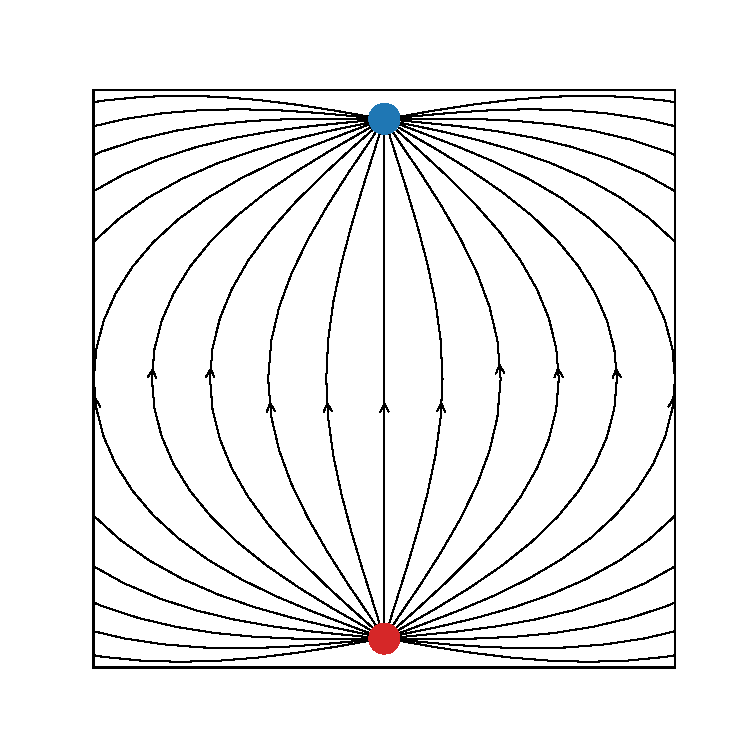
\includegraphics[width=0.3\textwidth]{figures/experiment/lhc/field-1.pdf}
}
\subcaptionbox{Quadrupole magnetic field\label{fig:magnetsB}}{
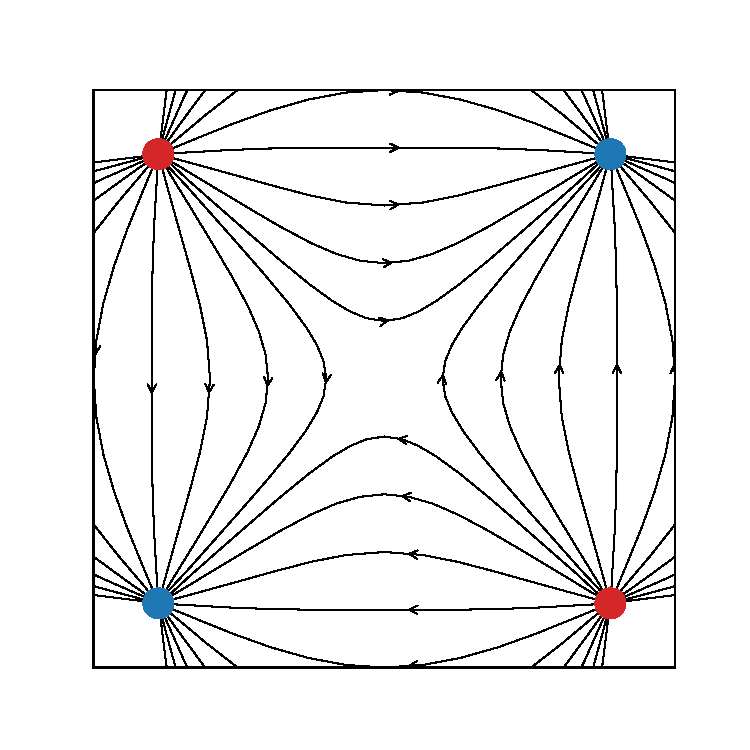
\includegraphics[width=0.3\textwidth]{figures/experiment/lhc/field-2.pdf}
}
\subcaptionbox{Sextupole magnetic field\label{fig:magnetsC}}{
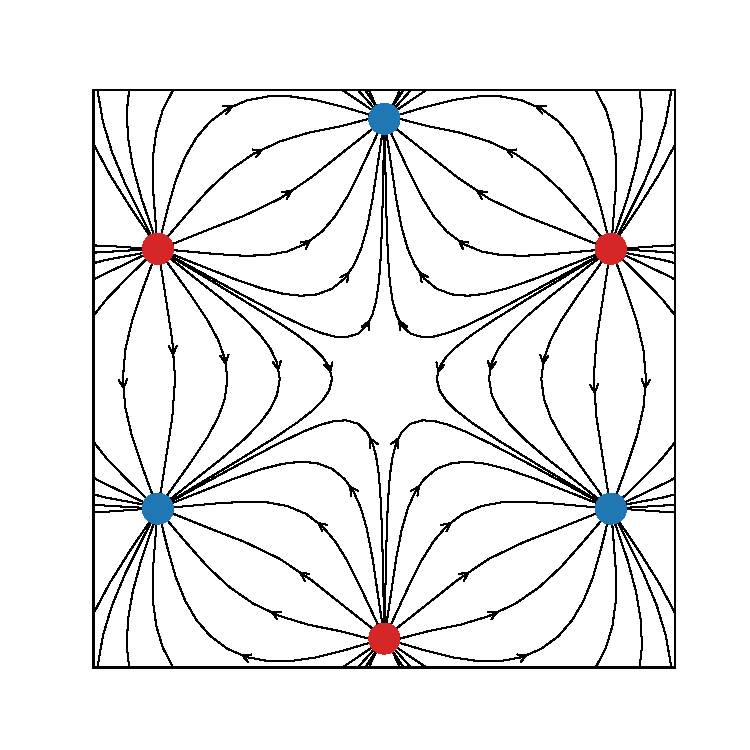
\includegraphics[width=0.3\textwidth]{figures/experiment/lhc/field-3.pdf}
}
\caption{Illustrations of the idealized fields of magnets used commonly in colliders. The poles of fields are shown in red (north) and blue (south). The density of the field lines indicates the strength while the arrows indicate the direction of the magnetic field. In a collider, the fields are orientated such that a particle beam's direction would be into the page.}
\label{fig:magnets}
\end{figure}

A number of magnets are used for a variety of purposes in a collider.
The most prevalent are dipole magnets used to guide the trajectory of the beam around the machine.
Dipole magnets have a nearly uniform magnetic field, $\pmb B$, as illustrated in Figure \ref{fig:magnetsA}
This leads to the circular motion of an incident particle with charge $q$, as described by Equation \ref{eqn:lorentzForce}.

In addition to dipole magnets, quadrupole magnets are used to focus and defocus the beam profile.
An illustration of a quadrupole field is given in Figure \ref{fig:magnetsB}.
A beam passing through a quadrupole is simultaneously focused in one plane and defocused and the perpendicular plane.
Quadrupole magnets are usually grouped in order to provide an overall focusing or defocusing effect on the beam.
A group of two quadrupoles, the second rotated 90 degrees from the first, have the effect of focusing a beam in both planes.

A third magnet configuration is the sextupole, consisting of an arrangement of three dipoles.
A sextupole is useful for adjusting the momentum dependant behavior of the beam. 
This is helpful in maintaining the stability and lifetime of the beam as it circulates the machine.
The field of a sextupole is illustrated in Figure \ref{fig:magnetsC}.

% \subsection{Colliding Beams}
The final task of a collider, after it reaches a stable beam energy, is to steer the beams into collisions.
As the particles making up the beam collide, they interact and transform the incident energy into an explosion of outgoing particles.
The locations of the collisions are such that the outgoing particles can be detected by an experiment.

\section{CERN Accelerator Complex}

\begin{figure}[h!]
\captionsetup[subfigure]{position=b}
\centering
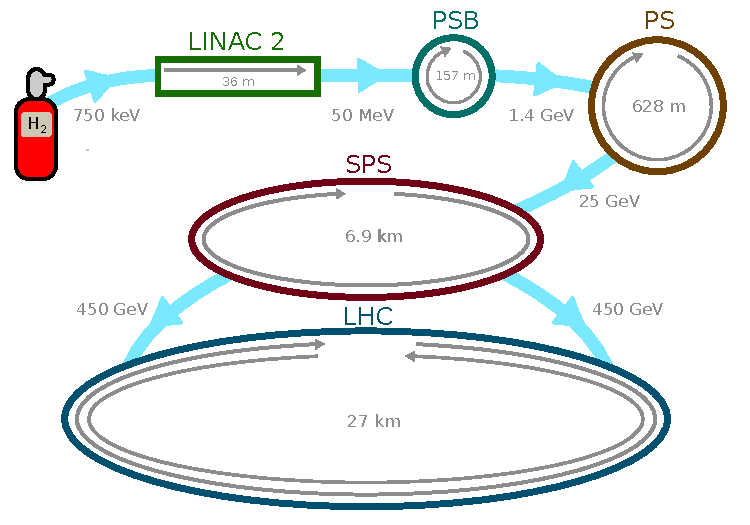
\includegraphics[width=0.8\textwidth]{figures/experiment/cernAccelChain.pdf}
\caption{A schematic view of the path taken by protons through CERN accelerator complex in order to produce beams at the LHC. The energy of the beam is labeled between each accelerator. The length or circumference of the accelerators are labeled, however the beam makes many orbits in each circular accelerator.}
\label{fig:accelComplex}
\end{figure}

The LHC requires input beams with high intensity and energy.
The LHC injector chain is tasked with providing this beam.
Four accelerators make up the chain: the Linac 2, the PS Booster, the PS, and the SPS.
The output of the chain is a proton beam with an energy of 450~GeV.
This section describes each of these machines and the proton beams that they produce \cite{schindl}.
The CERN accelerator complex, as it relates to the production of proton beams, is illustrated in Figure \ref{fig:accelComplex}.

% \subsection{Linac 2}
The first accelerator in the injector chain is the Linac 2.
Protons are sourced from a canister of hydrogen gas and separated by a 90~keV duoplasmatron ion source\footnote{A cathode emits electrons which ionize H$_2$ gas, separating the atoms, which are then accelerated electrostatically towards an anode.}.
The protons enter a 1~m RF quadrupole and are accelerated to 750~keV.
This beam enters the Linac 2, a linear accelerator which dates to 1978.
The Linac 2 accelerates protons to 50~MeV over the course of 36~m using a series of increasingly long RF cavities.

% \subsection{Proton Synchrotron Booster}
The beam output of the Linac 2 is transferred to the first in a series of synchrotrons called the \emph{Proton Synchrotron Booster} (PSB).
Synchrotrons are accelerators where the magnetic field strength is synchronized to the energy of the beam as it accelerates.
The PSB, which began construction in 1968, is a circular synchrotron with a circumference of 157~m.
The incoming beam from the Linac 2 is split vertically by an electrostatic deflector to four levels.
At this stage, the beams are divided into \emph{bunches} of protons, separated by empty space.
These four beams enter four circular rings stacked on top of each other, quadrupling the capacity of the PSB \footnote{The PS is designed to accept five bunches from each PSB ring for a total of 20 bunches. For LHC operation, it accepts one bunch from each PSB ring.} \cite{reich}.
The original PSB was renovated to provide beams for the LHC, and the output energy was increased from 800~MeV to 1.4~GeV. 
This helped reduce instabilities related to producing denser beams.
\cite{schindl}

% \subsection{Proton Synchrotron}
The four beamlines of the PSB are recombined and extracted to the \emph{Proton Synchrotron} (PS)\footnote{Originally named the CERN Proton Synchrotron (CPS).}.
The PS is a circular synchrotron with a circumference of 628~m, four times the circumference of each PSB ring. 
The PS was commissioned in 1959.
Significant effort was undertaken to prepare the PS to supply the beam for the LHC.
This included squeezing four bunches from each PSB ring into one half of the PS and filling the PS with two PSB cycles.
Once the PS has been filled and accelerated its beams to 25~GeV, the spacing between bunches is adjusted to match the LHC's requirements \cite{schindl}.

% \subsection{Super Proton Synchrotron}
The final accelerator before the LHC is the \emph{Super Proton Synchrotron} (SPS).
The SPS was completed in 1976 with a circumference of 6.9~km.
From 1981 to 1990, it provided beams to the UA1 and UA2 experiments, with which UA1 discovered the W and Z bosons.
As with the other CERN accelerators, the SPS underwent upgrades to provide beams to the LHC.
A total of 800 vacuum pumping ports were given Faraday shields to reduce interference caused by the interaction of the beam particles with the wall of the beamline \cite{schindl}.
Two new transfer tunnels were constructed as well to carry the beam from the SPS to ring of the LHC.
These lines carry two beams (clockwise and counter-clockwise) to the LHC, where they are injected into the main rings.

\section{The Large Hadron Collider}

Located in the Lemanic basin, straddling the border between Switzerland and France, the Large Hadron Collider is the largest machine built by humans.
There are seven experiments around the circumference of the LHC: four large experiments named CMS, ALICE, LHCb, and ATLAS, as well as three small experiments named TOTEM, MoEDAL, and LHCf.
The LHC provides the unique laboratory conditions required by ATLAS to investigate the fundamental nature of the Universe.
The construction, maintenance, and operation of the LHC are part of an enormous effort carried out by thousands of dedicated scientists and engineers.
Without their ongoing endeavors, the achievements of ATLAS and the other LHC experiments would be impossible.

The LHC is impressive not just in absolute terms, but also in comparison to previous accelerators.
The three other large superconducting accelerators, the Tevatron\footnote{Decommissioned in 2011.}, HERA\footnote{Decommissioned in 2007}, and RHIC, all operate with magnetic fields of approximately 5~T.
The main dipole magnets of the LHC surpass this with fields of 8~T.
The machine is also enormous; it has a circumference of 26.7~km.
The LHC, designed to reach collision energies of 14 TeV, is also the first hadron accelerator with enough synchrotron radiation to affect the design of the cooling and vacuum systems \cite{lyndon}.

The LHC is composed of several subsystems, each of which is complex and essential in its own right.
The magnet system bends and focuses the beam to maintain its stability over multiple hours.
The accelerator system uses radio-frequency chambers to accelerate the beams.
Various control systems monitor, collimate, and adjust the kinematics of the beam.
Finally, either in the event of a problem or once the beam has lost sufficient intensity, the beam is carefully disposed in the by the abort system.
This section describes how these systems collectively provide colliding beams inside the ATLAS experiment.

The LHC is a machine under continuous development; the only place to study improvements for the LHC is at the LHC itself.
As a result, the history of the LHC development is also the history of the experimental environment of the ATLAS detector.
This story begins with the tunnel and infrastructure that houses the LHC.

\subsection{Civil Engineering}

\begin{figure}[htb]
\captionsetup[subfigure]{position=b}
\centering
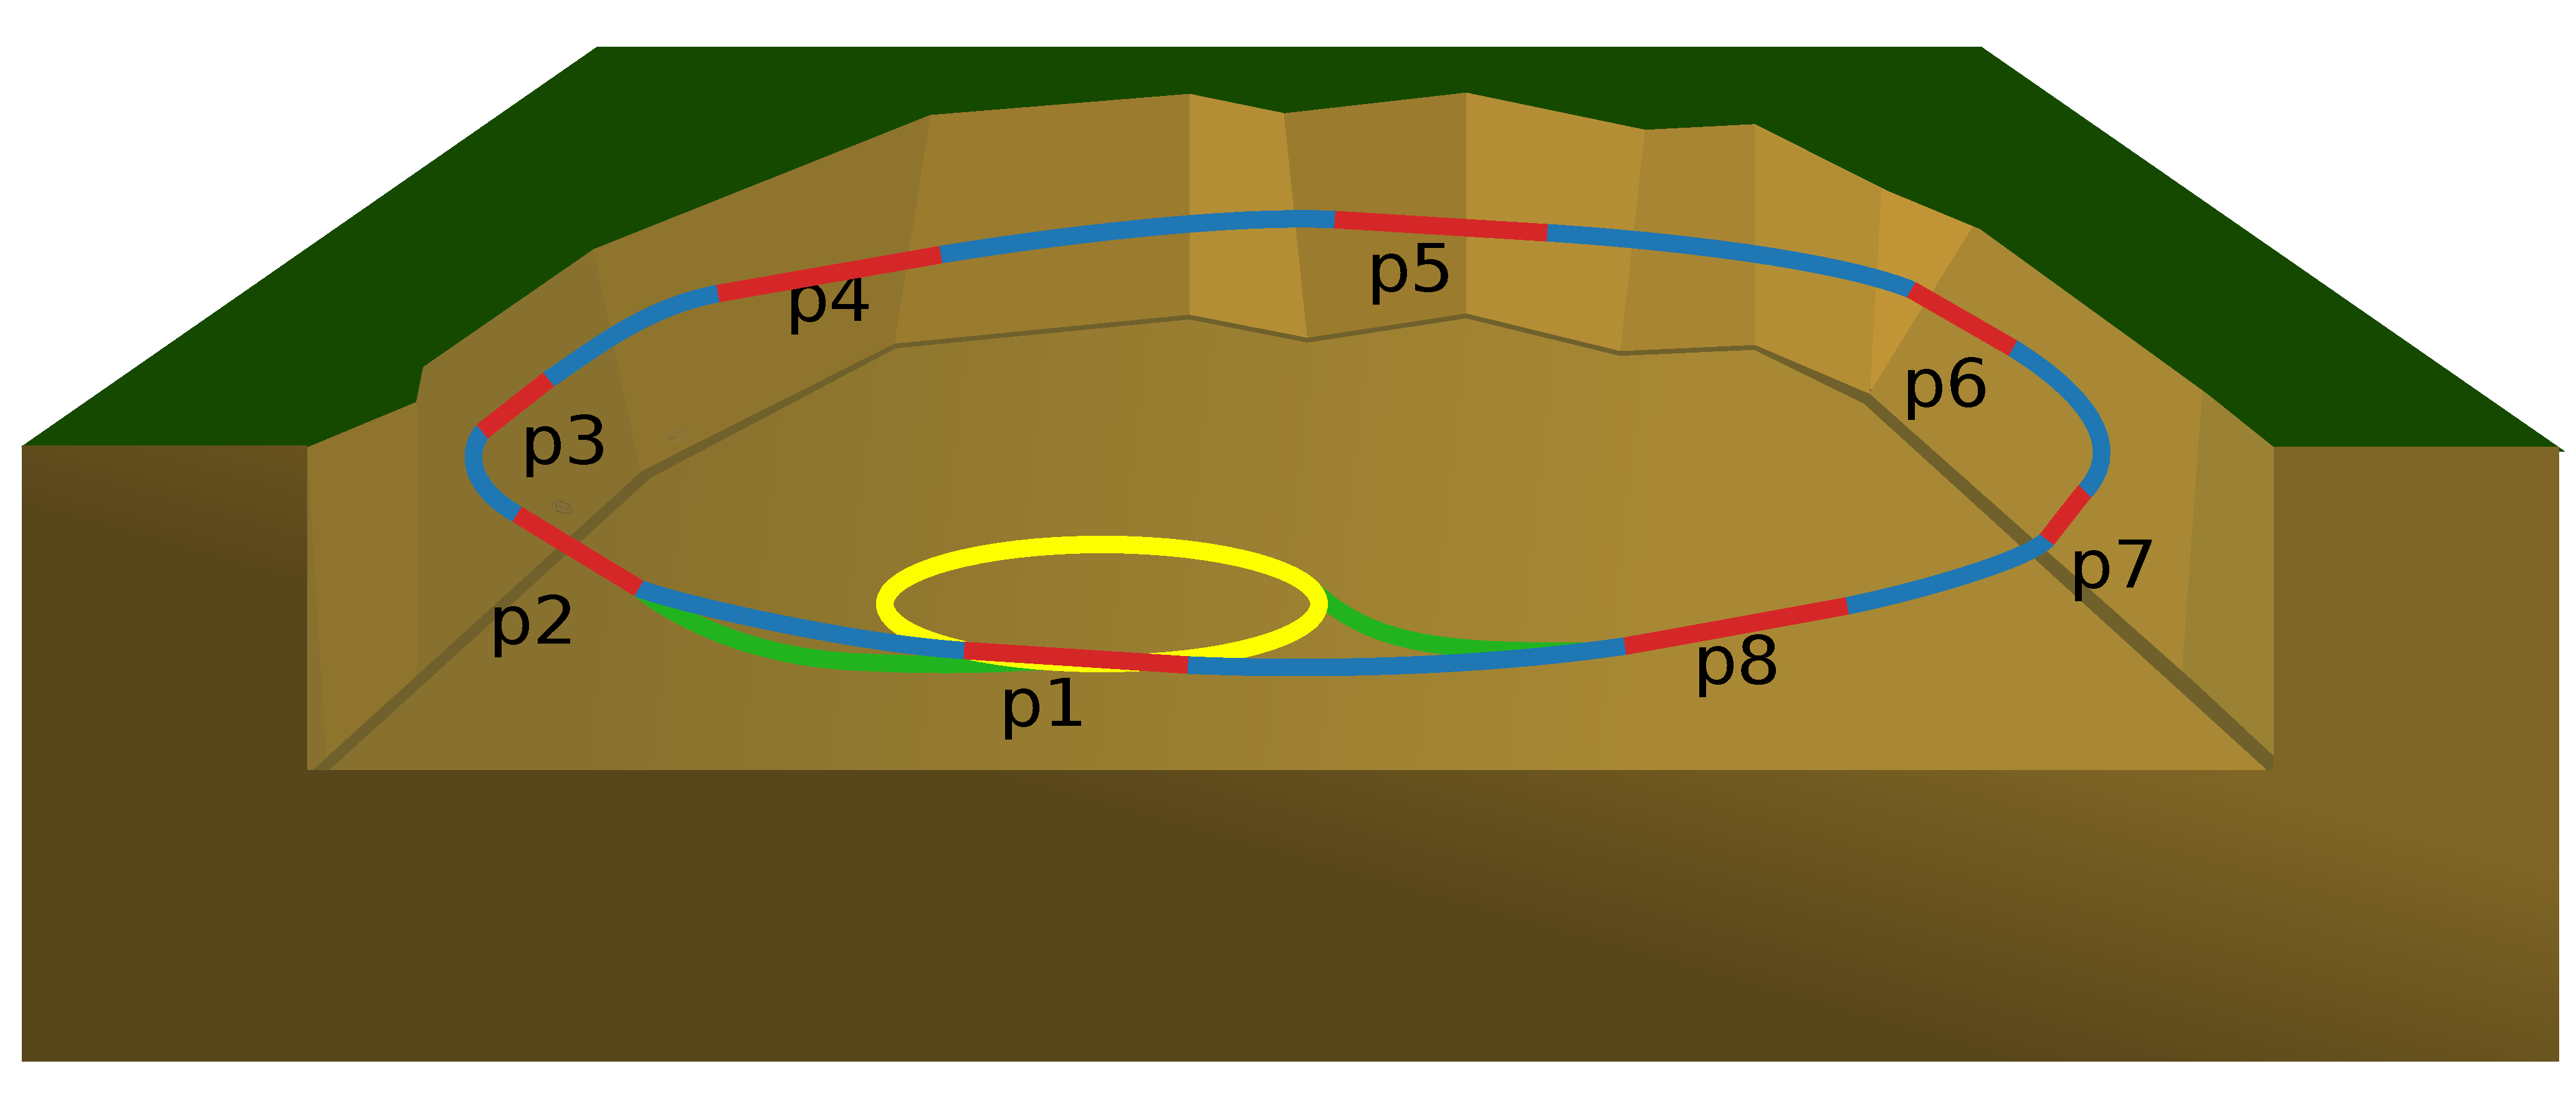
\includegraphics[width=0.9\textwidth]{figures/experiment/lhc/lhcMap.pdf}
\caption{Layout of the LHC, consisting of eight curved sections (blue) and eight straight sections (red) buried at a depth of 45-170~m. The location of SPS (yellow) and the injection lines (green) from the SPS are indicated.}
\label{figure:lhcLayout}
\end{figure}


The first step in building a collider is to construct civil infrastructure for it to inhabit.
This takes the form of a buildings that house services for the accelerator and a space for the machine itself.
For economic reasons, much of the infrastructure for the LHC is reused from the earlier LEP project.

The largest piece of infrastructure is the tunnel built to house LEP.
The Tevatron is buried less than 10~m deep in the flat expanse of the Illinois prairie.
This shallow tunnel could be constructed with a cut-and-fill approach.
RHIC is primarily built at surface level in a tunnel that was later covered with dirt.
Neither of these approaches was suitable in the context of the local geology in the region.
The land near CERN consists of a layer of moraine (loose unconsolidated rock) resting atop a layer of molasse (soft sedimentary rock).
LEP was buried in the sedimentary layer for stability, but this is too deep for excavation.
Instead, beginning in 1985, the tunnel was dug using tunnel bores and explosives.
In the Cenozoic molasse of the Lemanic basin, tunnel bores were used.
The bores were unsuitable for the fractured Mesozoic limestone beneath the Jura mountain and more costly explosives were used instead.
The resulting tunnel's internal diameter is 3.8~m, and it is buried at a depth of 45-170~m.
The tunnel slopes downward at 1.42 degrees in the direction of Lake Leman, in order to remain within the molasse layer.

The tunnel has eight curved arcs, separated by eight straight sections with length 528~m \cite{lyndon}.
Four straight sections house the ATLAS, CMS, ALICE, and LHCb experiments.
% The other four straight sections house the RF system, collimation controls, beam abort, and other utilities.
The eight straight sections, called points, are arrayed as shown in Figure \ref{figure:lhcLayout} and numbered p$i$ with $i\in\{1,...,8\}$.
The primary uses of each point is given in the following table.
\begin{center}
\begin{tabular}{c l l l}
\toprule
Location & Use \\
\midrule
    p1 & Hosts the ATLAS experiment \\
    p2 & Clockwise beam injection, and the ALICE experiment \\
    p3 & Hosts momentum collimation systems \\
    p4 & Hosts RF systems for acceleration \\
    p6 & Hosts beam abort, and beam dump \\
    p5 & Hosts the CMS and TOTEM experiments \\
    p7 & Hosts betatron collimation \\
    p8 & Counter-clockwise beam injection, and the LHCb experiment \\
\bottomrule
\end{tabular}
\end{center}
The eight curved sections host magnets with the purpose of bending the beam around the path of the machine.
The collider itself is built along the outer edge of the tunnel. In several locations, concentric outer tunnels house services for the accelerator.

After below-ground infrastructure, the next largest infrastructure for the LHC is surface buildings.
Every LEP building has been reused for the LHC, and some new infrastructure was built to accommodate the LHC.
First, a major expansion of the tunnels was undertaken to carry the beam from the SPS to the LHC injection points. Two new tunnels with an internal diameter of 3.75~m and a length of 2.5~km were dug to connect points p2 and p8 to the SPS.
While ALICE and LHCb reuse existing LEP era caverns, new caverns were built to house ATLAS and CMS.
In the cavern for CMS, the waterlogged moraine above the cavern had to be frozen with liquid nitrogen before excavation could be completed.
To avoid further flooding,\footnote{LEP flooded twice, at one time filling with 20~cm of sediment. A plan to waterproof the tunnel with a steel tube called ``the submarine'' was rejected.} existing draining tunnels were enlarged, and new tunnels were added.

In total, the construction of new infrastructure lasted five years.
\footnote{The CMS cavern construction was delayed past five years due to archaeological discoveries and the high water content of the soil. Eventually liquid nitrogen was pumped through tunnels dug through the soil to solidify it.}
Eight new surface buildings were constructed to hold offices and experimental equipment. 
Work at p1 for the three ATLAS caverns began in April of 1998 \cite{lhcDesignV2}.
Four new shafts, two over the experimental cavern and one over each service cavern, were excavated.
The ATLAS experiment cavern is built 92~m below ground. 
To house the large experiment, 300,000 tonnes of rock were removed to clear an area 53~m long, 30~m wide, and 35~m tall.
The walls and ceiling are constructed from 2~m thick concrete, and the floor is 5~m thick to support the 7,000 tonne detector.


\subsection{Accelerator Design}
The heart of the LHC is the accelerator.
The purpose of this system is to accelerate beams to their collision energy and then maintain their energy to compensate for losses over time.
% Beams are accelerated only in a short section of p4.
The circular design of the LHC means that beams repeatedly pass through the same acceleration section.
As a result, the acceleration system need only impart 3.7 kW/beam rotation.
% During the design operation, synchrotron radiation energy loss is 3.7 kW/beam: not much acceleration is lost in a revolution.
% The acceleration system needs only to make up for a small amount of lost energy per turn.

The principle of acceleration is based on radio-frequency (RF) cavities.
Independent RF systems control the acceleration of each beam circulating in opposite directions.
% Each cavity provides 32kW to increase the beam energy.
Cavities are made of copper, sputtered with niobium.\footnote{In magnetron sputtering used for this process, niobium is vaporized by particle bombardment and bound to the copper substrate of the cavity resulting in a thin - and inexpensive - 1-2 micron coating.}
This is advantageous over solid niobium for its thermal conductivity and its superconductivity to enhance the RF performance \cite{lyndon}.
The operation of the superconducting cavities requires temperatures of 4.5~k, so cavities are enclosed in cryomodules with their own helium tanks \cite{boussard}.
The resonant properties of the cavities can be adjusted during operation by mechanically distorting their shape.

Each cavity operates with a voltage of 2~MV (5.3 MV/m) and is powered by a 500~kW klystron.
The klystrons are coupled to the cavities by a waveguide of adjustable length.
Adjusting the length of the waveguide, in turn, adjusts the \emph{quality factor}\footnote{Peak energy lost per cycle, which can be used to adjust the peak voltage in the cavity.} of the cavity.
The cavity is kept at a 3~kV bias to reduce the rate of electron avalanches (multipactor effect).
During normal operation, the klystrons drive the cavities at 400~MHz and supply 200~kW.

\begin{figure}[h!]
\captionsetup[subfigure]{position=b}
\centering
    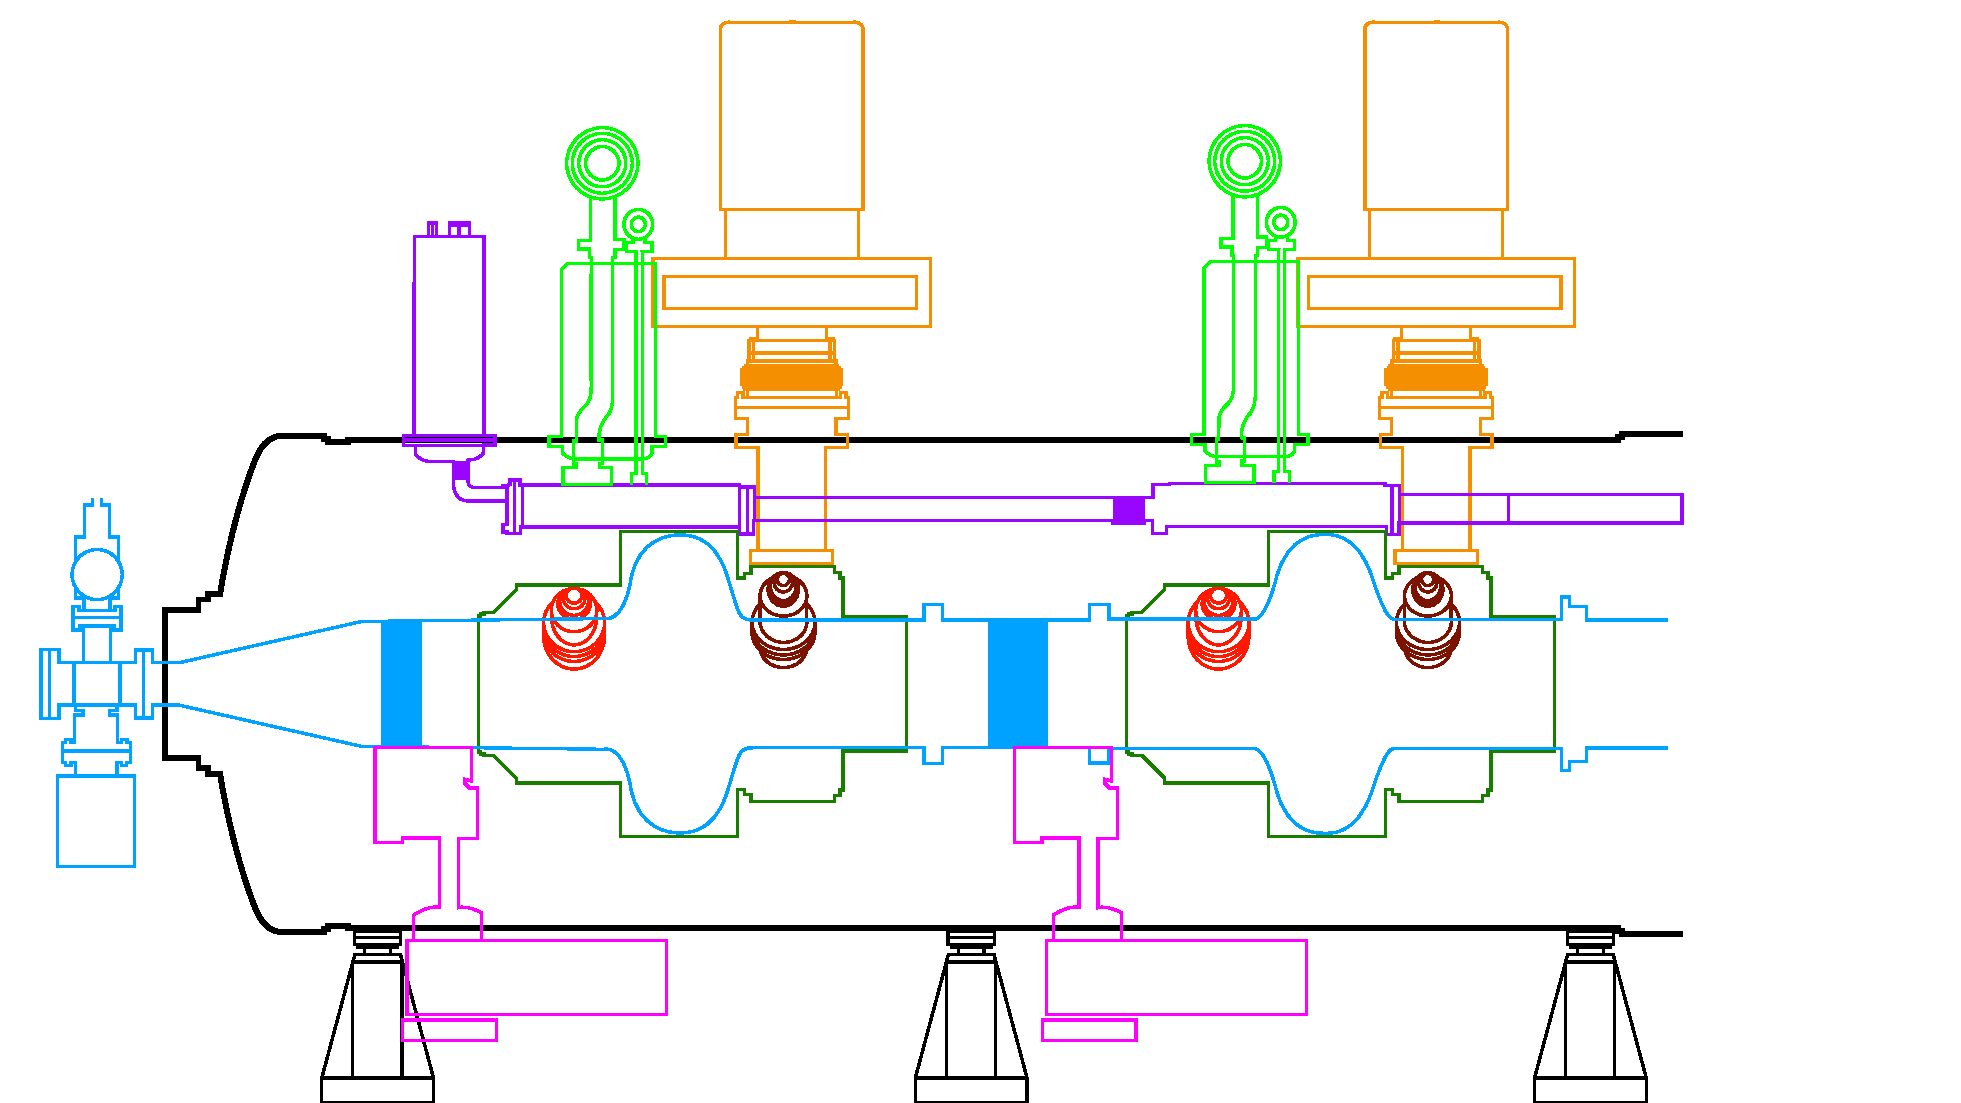
\includegraphics[width=1\textwidth]{figures/experiment/rfproto.pdf}
    % 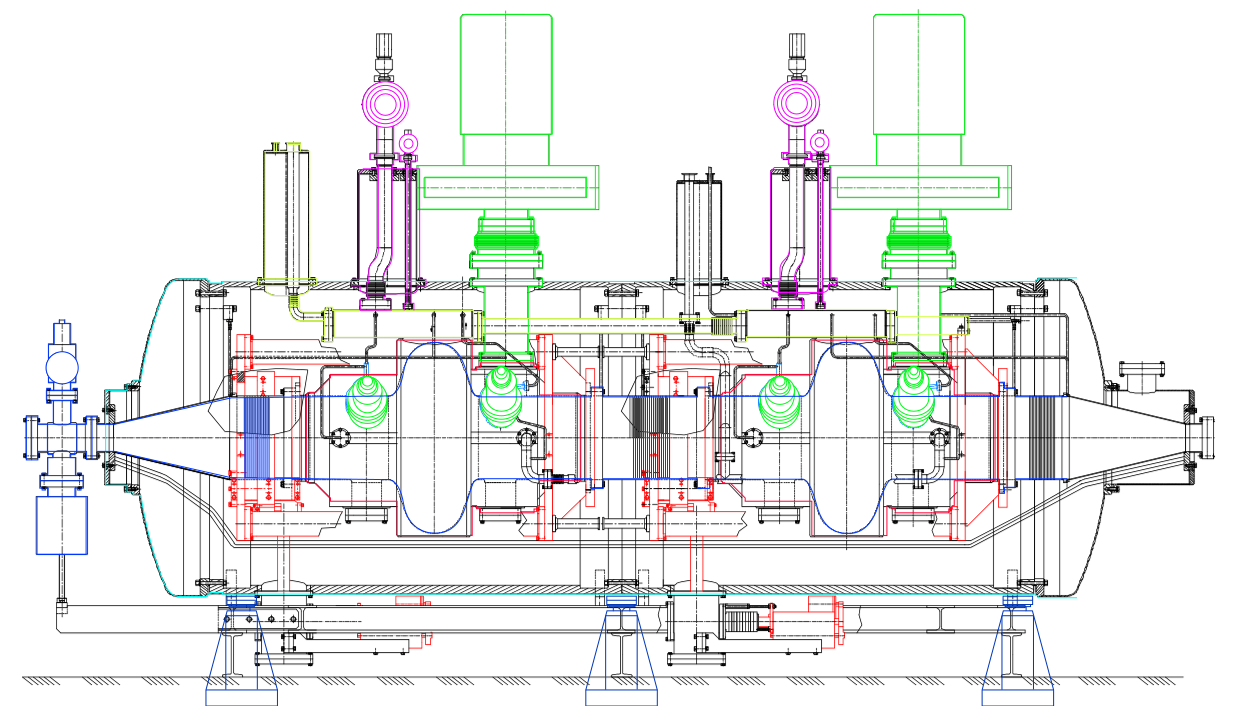
\includegraphics[width=1\textwidth]{figures/experiment/rfproto.png}
\caption{Schematic side-view of an LHC accelerating module showing two of the four cavities (blue). The cylindrical vacuum tank is shown in black. Inside, the beamline is shown in blue. The cavities are housed inside helium-filled cryomodules (dark green) fed by liquid helium baths (purple). Quench valves attached to the helium baths are shown in light green. Each super conducting cavity is driven by the variable power couplers shown in orange. Two other couplers control the higher order resonance modes in the cavity: a broadband HOM coupler (red) and a narrow band HOM coupler (brown). The resonance of each cavity is tuned by elastic deformation of the chamber by a motor system (pink).}
\label{fig:cavities}
\end{figure}

There are eight single-cell cavities per beam.
Four cavities are grouped to share a single cryostat, which maintains their superconducting temperature.
The resulting total voltage gradient is 16~MV per beam.
A schematic of the accelerator system is shown in Figure \ref{fig:cavities}.
The driving frequency is supplied through the couplings on top of the cryostat.
The cryostats are too large to sit next to each other in the tunnel, so they are staggered.

\subsection{Magnet Design}
If the accelerator is the heart of the LHC, the magnets compose its body.
Magnets serve multiple purposes in handling the beam.
A total of 1,232 dipole magnets bend the beam around the circumference of the collider.
Quadrupole magnets focus and defocus the beam as it travels. Each quadrupole simultaneously focuses in one direction and defocuses in an orthogonal direction. There are 392 quadrupoles throughout the curved arcs.
Sextupole magnets correct beam characteristics including chromaticity introduced by the quadrupoles. There are 2464 sextupole magnets in total.
Finally, other magnets such as octupole and decapole correctors fill in the remaining 7000 superconducting magnets of the LHC.
Together these magnets steer the beam into the LHC and maintain the beam's orbit during collisions.
At the end of the beam's lifetime, kicker magnets steer the beam safely into the beamdump.

\begin{figure}[h!]
\captionsetup[subfigure]{position=b}
\centering
\subcaptionbox{Coil winding \label{fig:lhcCoils}}{
    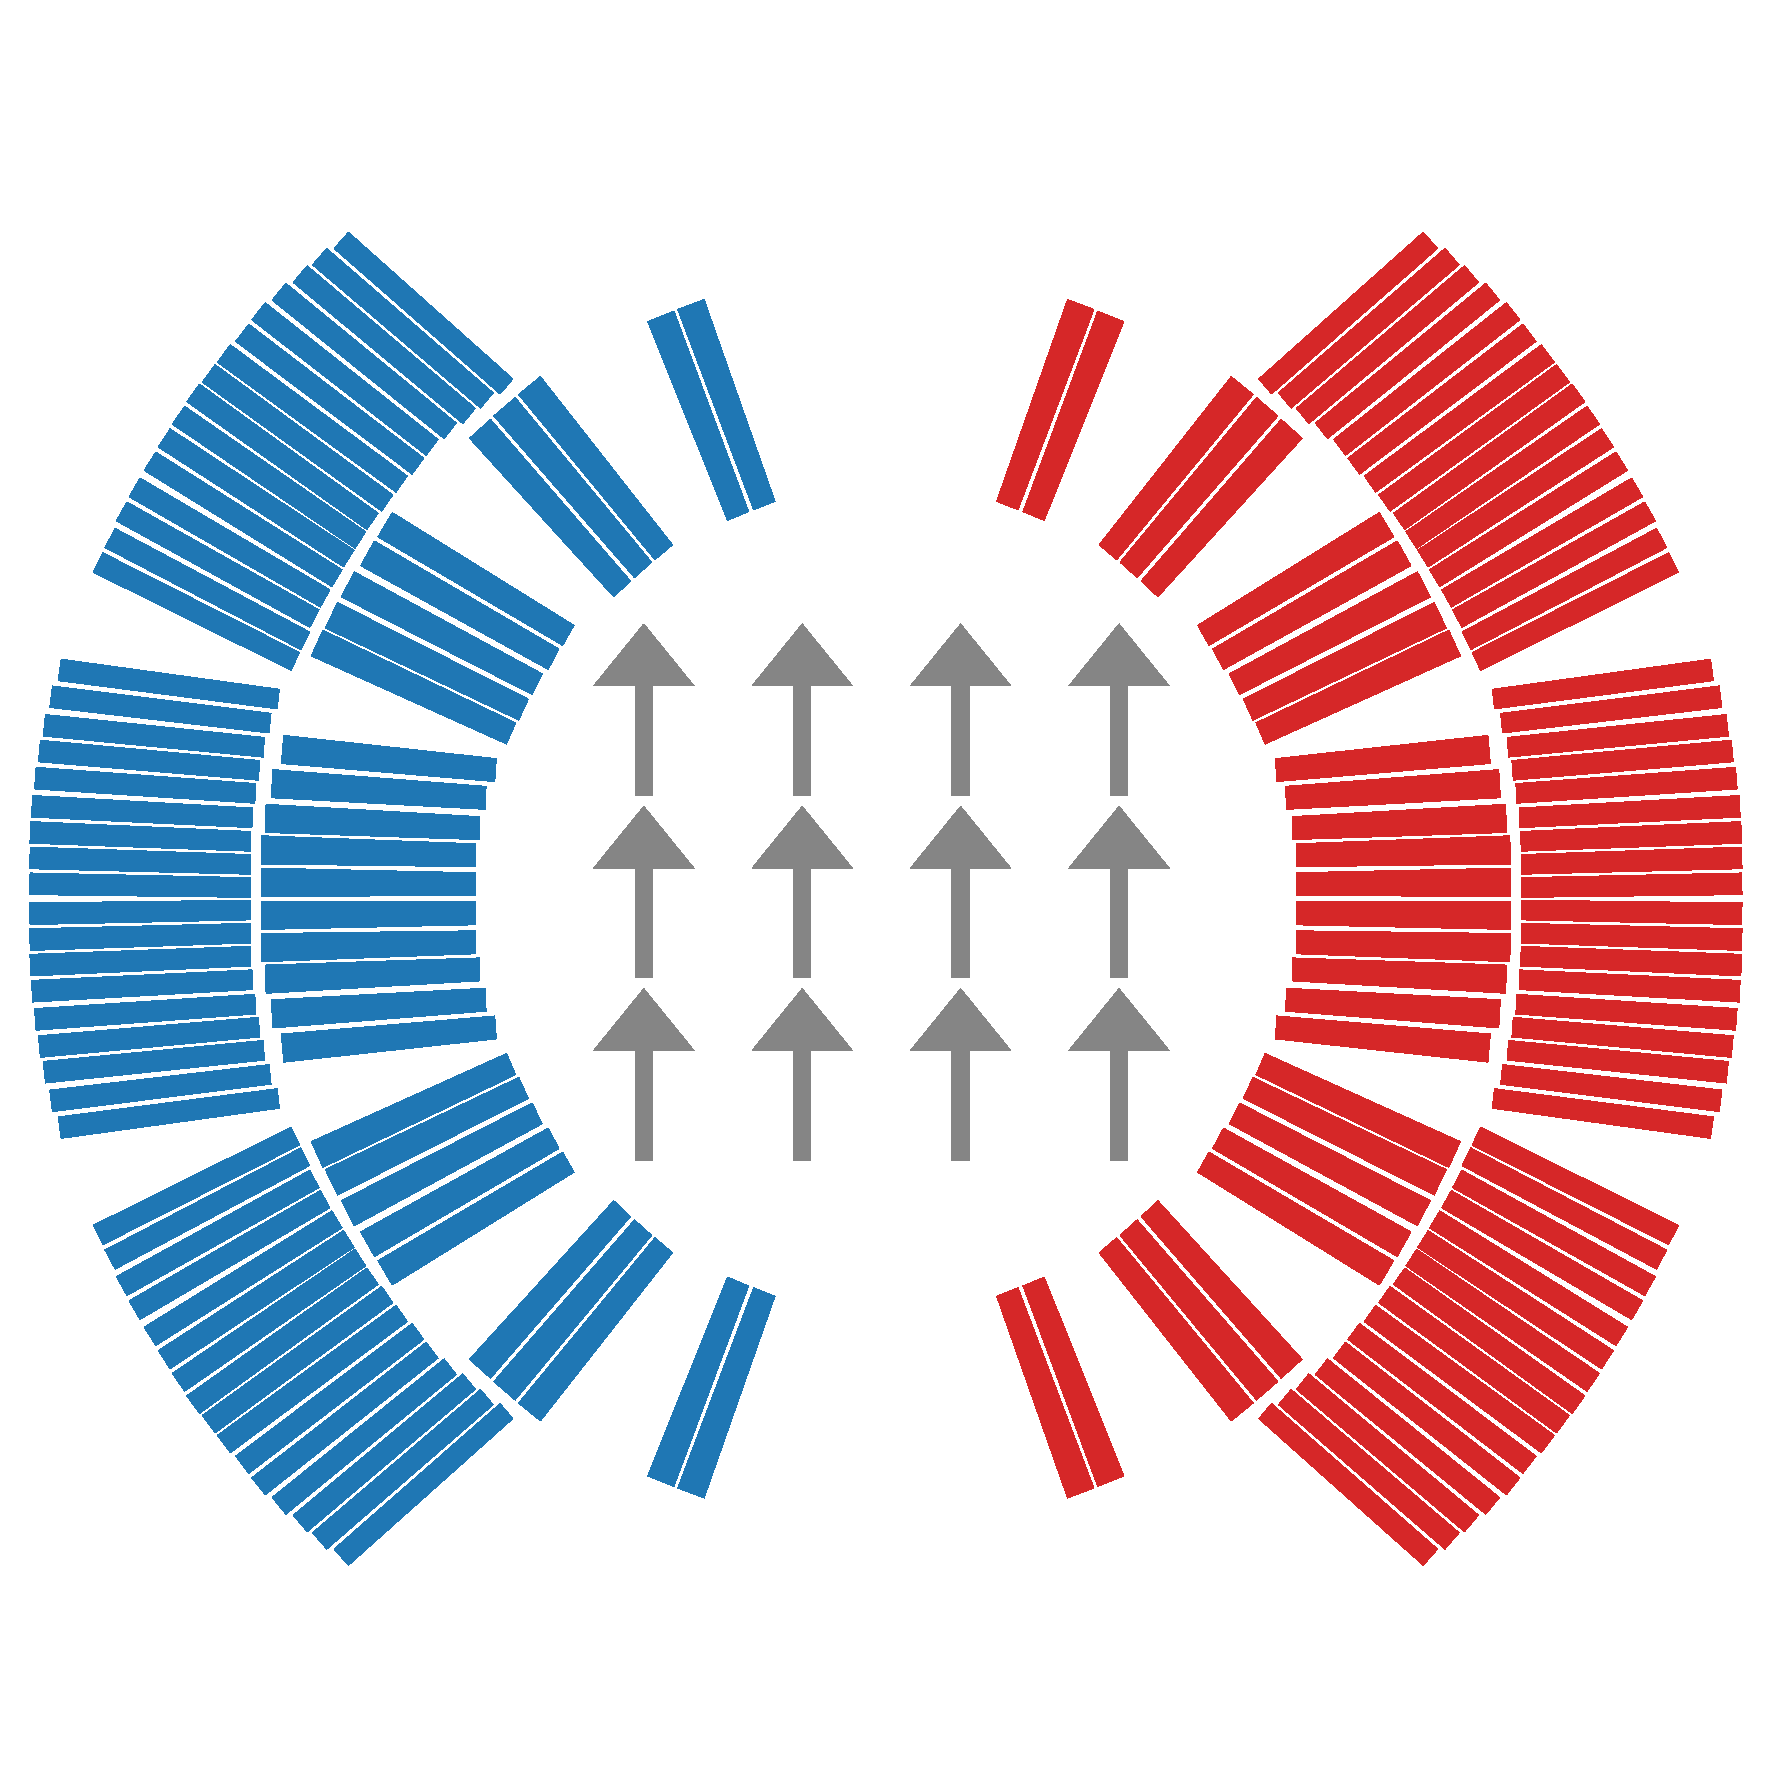
\includegraphics[width=0.4\textwidth]{figures/experiment/lhcCoils.pdf}
}
\subcaptionbox{Dipole magnet \label{fig:dipoleMagnetLhc}}{
    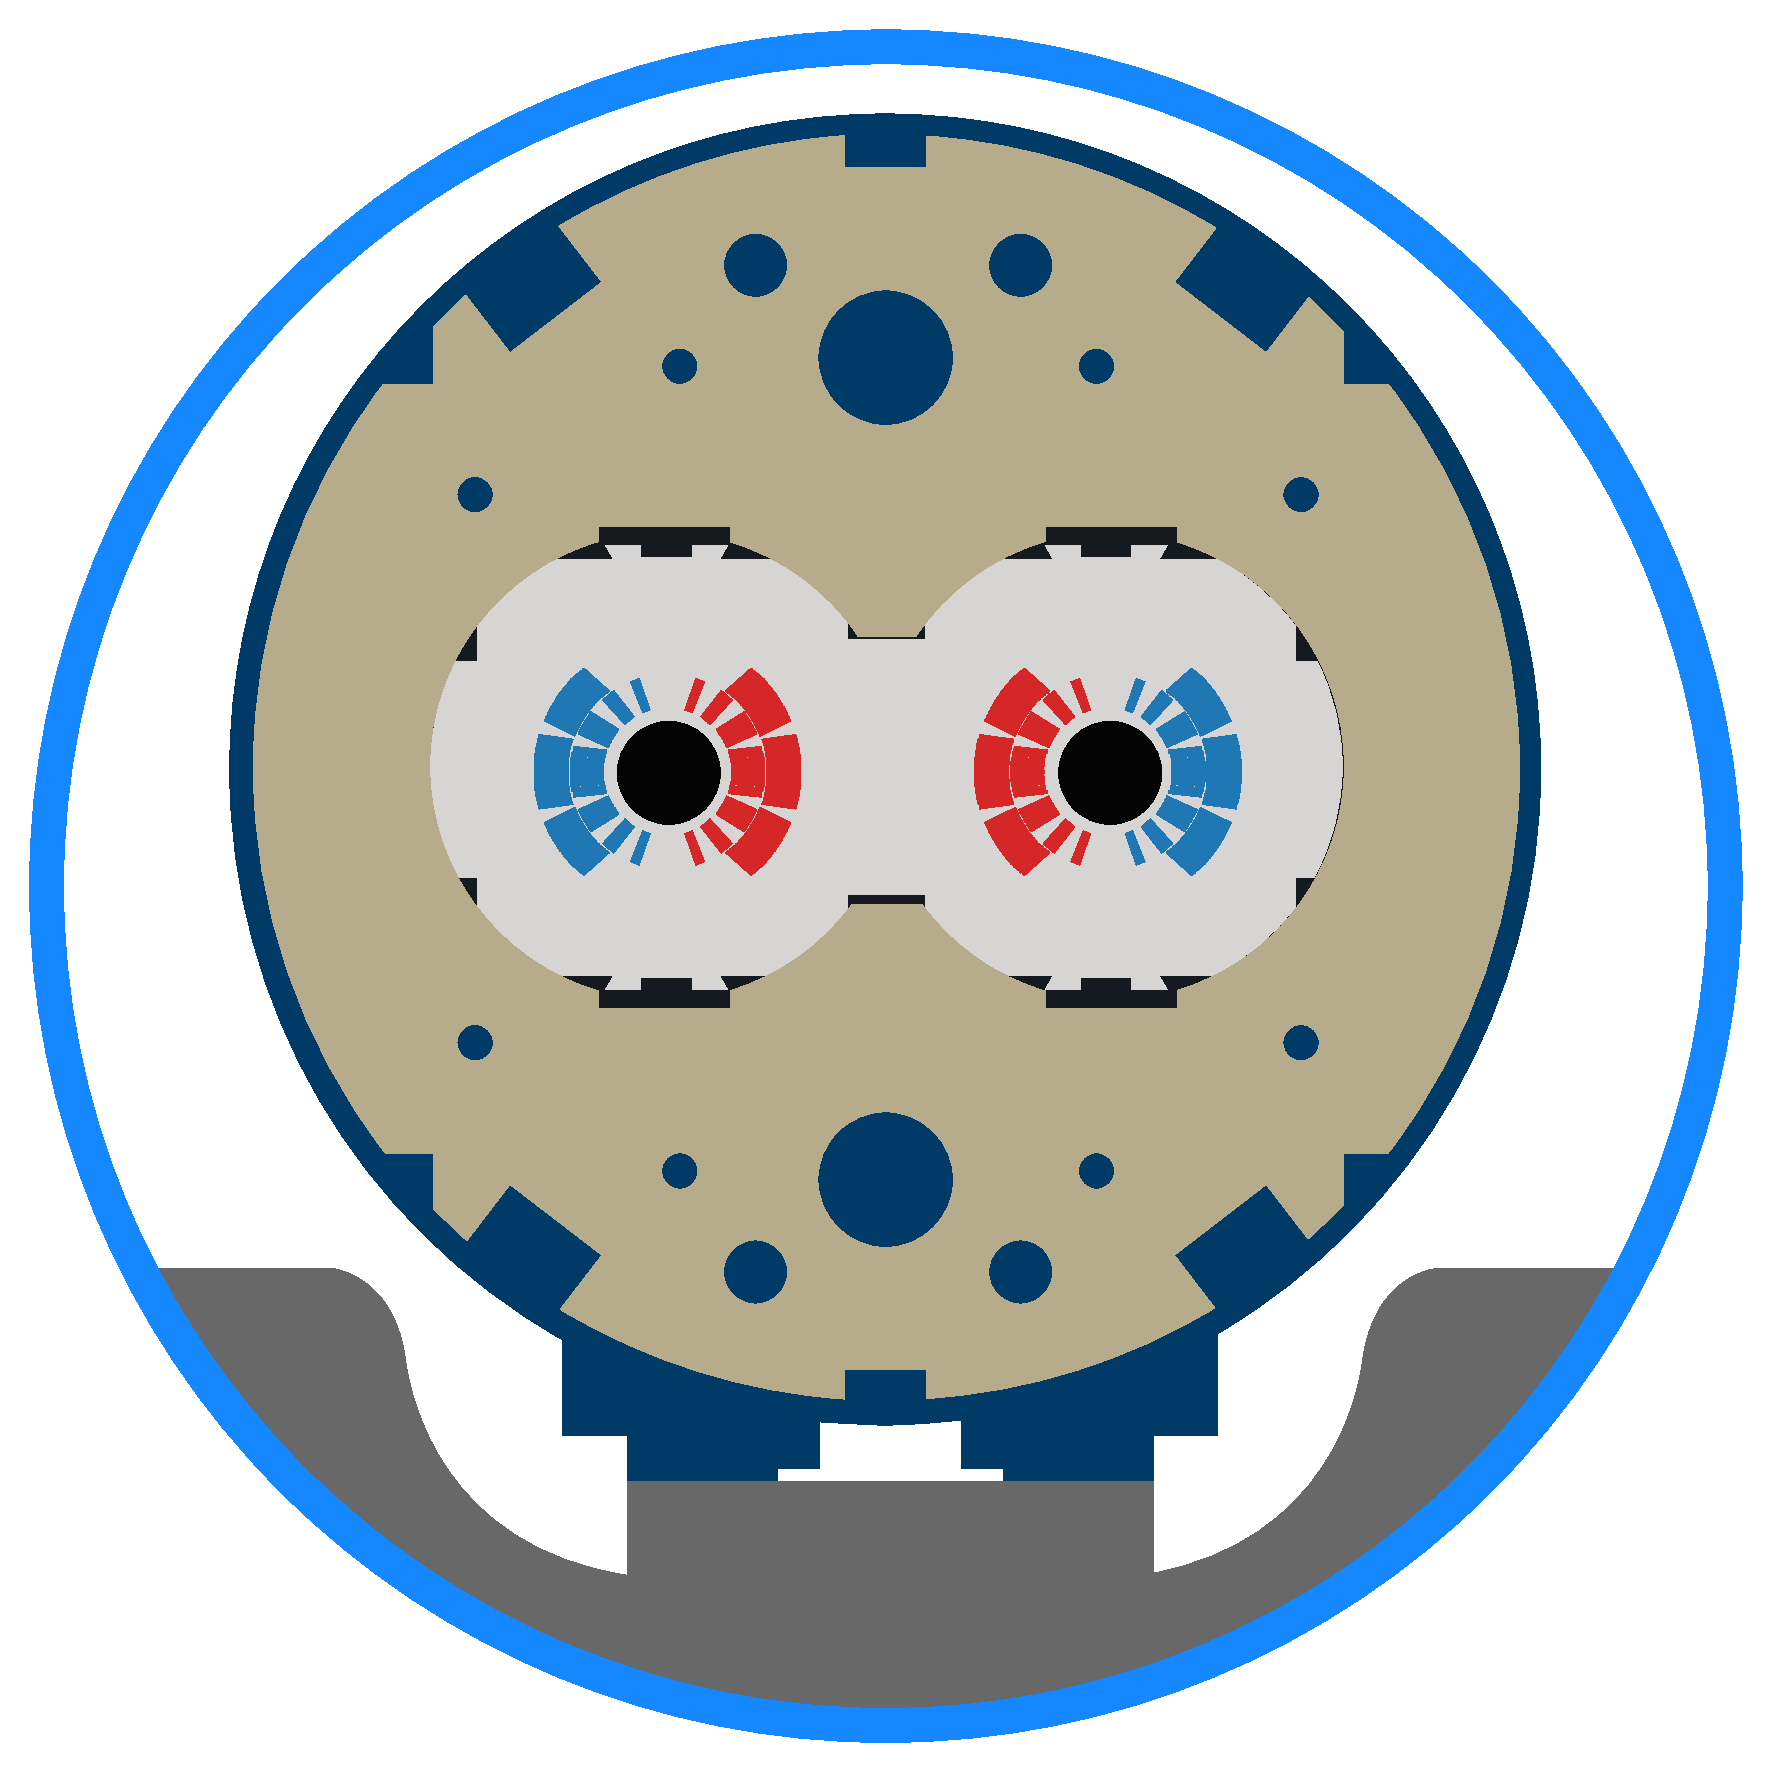
\includegraphics[width=0.4\textwidth]{figures/experiment/lhcMagnet.pdf}
}
\caption{(a) Cross section of the coils made from superconductive cables wound around the beamline to produce a homogeneous dipole magnetic field. Each rectangle represents a flat Nb-Ti cable. These are grouped in a configuration that produces a smooth internal magnetic field, indicated by the arrows. The cables are separated by layers of copper. The cables are color coded: red(blue) cables carry current into(out of) the page. (b) Cross section of the main bending dipole magnets. Two beamlines (black) and coils (blue/red) are are encased by austenitic steel collars (light grey). The collar is embedded in a large iron yoke (dark grey) and submerged in a liquid helium vessel (dark blue). The arrangement is held in a cryostat. For scale, the centers of the beamlines are separated by 19~cm.
}
\label{fig:dipoleFlux}
\end{figure}

% Dipole system
The dipole magnets perform the job of bending the beam around the LHC.
Because the counter circulating beams are both positively charged, magnetic fields of opposite directions are needed to steer them.
In the dipole magnets, two sets of superconducting coils are wound from flat cables with trapezoidal cross sections.
Each cable is made from 28-36 strands of $\approx1$~mm diameter stranded niobium-titanium (Nb-Ti) alloy wires.
\footnote{Although niobium-tin (Nb$_3$Si) has many desirable advantages over Nb-Ti, it is brittle and requires many hours of heat treatment at a temperature of $\approx$970~k. Alternatively, Nb-Ti has a low heat capacity at 1.8~k, so it is susceptible to rapid heating and quenching}
The coils are arranged in inner and outer layers, as shown in Figure \ref{fig:lhcCoils}.
This configuration produces a homogeneous, purely dipole field.
The coils for each beam are positioned side-by-side, such that the field of one can augment that of the other.
These coils share a common yoke made from low carbon steel with high magnetic permeability, chosen to conduct the magnetic flux between the coils.
This is illustrated by the black arrows in Figure \ref{fig:dipoleMagnetLhc}.
The coil and yoke assembly is held in place by collar plates of austenitic (low permeability) steel.
The resulting magnetic field has an incredible strength of 8.3~T.
Each of the main dipole magnets has a length of 14.2~m (15~m, including connections between the magnets).

% Cryosystem
In order to operate at superconducting temperatures, the magnets are housed elaborate inside cryosystems that regulate their temperature.
These are challenging systems: during the LHC's Run 1, the cryosystem was responsible for 25-30\% of fault time \cite{lhcRun1}.
It is the task of the cryosystem to maintain the magnet at 1.9~K using superfluid helium. A total of 100 tons is used throughout the LHC.
Helium is used because its low viscosity allows it to permeate the coil insulation and contact directly with the superconducting wire.
Superfluid helium has a specific heat roughly 2,000 times that of the Nb-Ti; this has the important benefit of increasing the system's total specific heat.
Helium is also effective at quickly transporting heat away from the wire.
The magnets are submerged in a bath of 1~bar liquid helium. A pipe is pumped with low pressure 15~mbar liquid helium to pull heat away from the bath.
This is done to prevent vapor bubbles from developing in the bath, leading to the coil heating and subsequent quenching.
In the event of a quench, a capacitor bank is fired into series with the coil's circuit to quickly add resistivity. The current is diverted through a diode while the power is ramped down.

Magnets are grouped into ``periods'' with identical magnetic properties.
Each period is 106.9~m long and consists of six main dipoles and two 6.6~m ``short straight sections'' (SSS).
Each SSS contains quadrupole magnets that re-focus the beam after being steered by the dipoles.
Additionally, each SSS also contains sextupoles that control chromaticity and small dipoles for orbit corrections.
Some SSS also contain octupoles and trip/skew quadrupoles for fine-tuning the beam characteristics.
Perturbations in the trajectory of the beam are introduced by the magnets and are called \emph{dispersion}.
After completing one of the eight arcs, the magnet of the dispersion suppressor system cancels the horizontal dispersion introduced during the bending.

\subsection{Beam Structure and Design}
The achievement of building the LHC pales in comparison to the achievement of producing and maintaining its beams.
The LHC was designed to collide two counter-rotating beams, at precise locations, with the enormous instantaneous luminosity of $10^{34}cm^{-2}s^{-1}$.
The energy of each beam exceeds that of a large truck traveling at highway speeds.
This is more than one hundredfold the stored beam energy of any previous machine \cite{lyndon}.
The beam is an object of enormous energy and surpassing delicacy.
Numerous technical considerations must be addressed in order for the beam to be useful for the experiments.
The beams at the LHC are characterized by several parameters that describe their stability and utility.
These parameters are described in this section.

The first parameter to consider is the \emph{emittance}, $\epsilon$, defined in Equation \ref{eqn:emittance}.
It is a measure of the distribution of the particles in a beam in position-momentum phase space.
The emittance is defined as
\begin{equation}\begin{split}\label{eqn:emittance}
\epsilon \equiv \frac{6\pi}{B}\left(w^2-D^2\left(\frac{dp}{p}\right)^2\right),
\end{split}\end{equation} 
where $w$ is the RMS beam width, $D$ is the dispersion, $B\approx(w/\epsilon)$ is the beta function, and $\frac{dp}{p}$ is the relative momentum spread.
The emittance is often divided into longitudinal and transverse components.
If the emittance is too small, then intra-beam interactions destabilize the beam. 
During injection, the beam has a longitudinal emittance of 0.6-1 eV, and this is increased to 2.5 eV during acceleration for stability.
Conversely, if the transverse emittance is too large, colliding beams pass through each other without interacting.
\cite{boussard,lyndon,pdg2016}

\begin{figure}[h!]
\captionsetup[subfigure]{position=b}
\centering
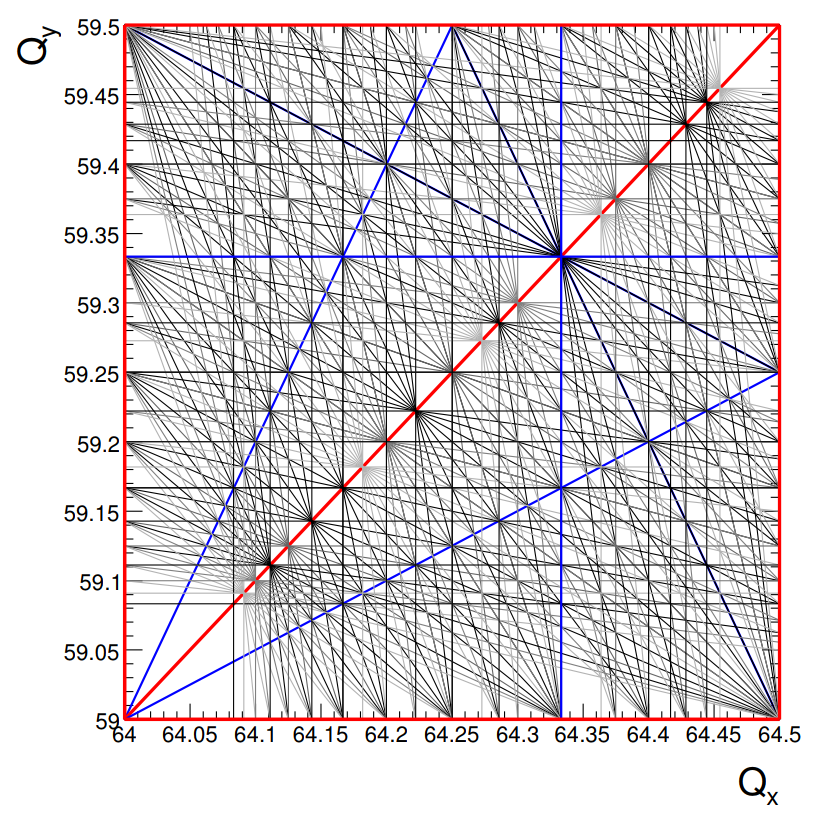
\includegraphics[width=0.4\textwidth]{figures/experiment/tune.png}
\caption{Tune diagram for the LHC. The horizontal and vertical tunes are displayed. First order resonances shown in red, second order resonances shown in blue, and higher order resonances shown in black. Figure from \emph{Tune and Chromaticity Diagnostics} \cite{steinhagen}}
\label{fig:tune}
\end{figure}

Related to the transverse emittance are \emph{betatron oscillations}: harmonic motion in the transverse plane as the beam makes an orbit \cite{pdg2016}.
This is a problematic source of intra-beam scattering of protons through coulomb forces.
The frequency of betatron oscillations is higher than that of the orbit.
The number of vertical or horizontal betatron oscillations made during one orbit is called the vertical or horizontal \emph{tune}, respectively.
The horizontal and vertical tunes must be carefully picked using a tune diagram, as exemplified in Figure \ref{fig:tune}.
Resonances are illustrated as lines, and the tunes must be selected together to avoid disruptive resonances.
The beam density, $N$, as well as emittance and $\beta$ modify the tune tune $Q$:
\begin{equation}\begin{split}
    \delta Q\propto-\frac{N}{\beta\gamma^2\epsilon^*}.
\end{split}\end{equation} 
For example, when the PSB was renovated the emittance was reduced, and the energy ($\gamma$) was increased to compensate for the impact on tune.
In practice, tunes are adjusted continually by adjusting these parameters throughout beam injection, ramping up beam energy, and eventual collisions.

Related to the longitudinal emittance are \emph{synchrotron oscillations}: longitudinal oscillations along the direction of the beam.
This takes place at a much lower frequency than that of betatron oscillations: at the LHC it is less than one oscillation per orbit.
As with betatron oscillations, the synchrotron oscillation frequency must be carefully controlled to limit intra-beam scattering and maintain beam stability \cite{pdg2016}.

\emph{Chromaticity} describes the dependence of the tune on a change of momentum.
In optics, light rays of different wavelengths are focused differently by a glass focusing lens.
There is a persistent analogy between optics and beam dynamics (often called beam optics). Like light, beams are bent and focused by magnets. 
Particles with large momentum experience weaker focusing strength from focusing quadrupoles, a process called \emph{chromatic aberration}.
Chromaticity quantifies this momentum dependence.
To put it explicitly, chromaticity $Q'$ is the tune change $\Delta Q$ caused by a relative momentum change $\Delta p/p$ \cite{fuchsberger}.
\begin{equation}
    \Delta Q = Q'\frac{\Delta p}{p},
\end{equation}
where
\begin{equation}
\begin{split}
    \frac{\Delta p}{p} = \frac{\Delta f/f}{\eta}; \quad\text{and}\quad \eta = \frac{1}{\gamma_r}-\alpha_c. \\
\end{split}
\end{equation}
Here, $\Delta f$ is change in RF frequency, and $f$ is the nominal frequency \footnote{400,788,860 Hz at the LHC.} 
$\gamma_r$ is relativistic gamma function, and $\alpha_c$ is momentum compaction factor equal to $3.225\times10^{-4}$ at the LHC.
Chromaticity is unitless as it defines a change in the tune.
At the LHC, sextupoles control the beam's correct chromatic aberration after passing through focusing quadrupoles and dispersion suppression \cite{frascati} \cite{bruno}.
The chromaticity is visualized on a tune diagram, such as Figure \ref{fig:tune}, as the area occupied by the beam.
Reducing the beam's chromaticity makes it easier to find a stable setting for the tune.
% From Jorg
However, beams with a chromaticity that is too small suffer from instability related interaction with the beampipe.
The momentum spread of a beam with high chromaticity makes it more efficient to absorb reflected EM fields without perturbing the beam.
An important task is to find a balance for the chromaticity in order to maximize the useful life of the beam.

% Bunches
Because the RF cavities produce alternating field gradients, the beam is naturally organized into occupied \emph{bunches} and empty space.
The time interval between these, the bunch spacing, is a multiple of the RF frequency.
At the LHC the nominal bunch spacing is 24.96~ns, or ten times the RF frequency. The corresponding bunch length is 7.5~cm \cite{boussard}.
Bunches are collected into trains, patterns of occupied and empty bunches.
Several trains comprise the beam.
Several bunches are always left unoccupied, called the abort gap. The length of the gap corresponds to the ramp time of the extraction kicker magnet.
The bunch design choice depends on the function of the beam. Some patterns are useful for cleaning the beampipe of electron clouds, while others are useful for optimizing physics collisions.

% Lumi
From a physics perspective, the most important beam characteristic is the instantaneous luminosity of collisions.
This is defined as $L\equiv N/\sigma_{pp}$, where $N$ is the collisions per second and $\sigma_{pp}$ is the poorly defined proton-proton collision cross-section\footnote{This is poorly defined because in some sense protons always scatter off each other, so the definition depends on what constitutes a collision. Traditionally, values of $\sigma_{pp}\sim10^{14}\text{fb}$ are used.} \cite{lyndon}
More precisely in the context of the LHC, the luminosity is defined in Equation \ref{eqn:lumi} \cite{lyndon}.
\begin{equation}\label{eqn:lumi}
    L=\frac{N_b^2nf_r\gamma}{4\pi\epsilon_n\beta^*}
\end{equation}
Here, $N_b$ is number of particles per bunch, and $n$ is the number of bunches per beam.
$f_r$ is is revolution frequency, which is 11.245 kHz for the LHC.
The other terms are the previously mentioned relativistic $\gamma$, the transverse emittance $\epsilon_n$, and the beta function at the collision point $\beta^*$.
The two beams must be steered into each other at a crossing angle of $\theta_c$.
This results in a luminosity reduction factor,
\begin{equation}\label{eqn:lumiReduce}
    F=1/\sqrt{1+\frac{\theta_c\sigma_Z}{2\sigma^*}}
\end{equation}
where $\sigma_z$ is the RMS bunch length, and $\sigma^*$ is the transverse RMS beam size at the interaction point.
In fact, $\sigma^*$ is specifically minimized by focusing the beam before the collisions and defocusing it afterward.

The central challenge during the operation of the LHC is to keep the beam in a stable orbit for many hours.
Several effects may purturb the stability of the beam during this time \cite{lyndon}.
\emph{Beam-beam interaction} is the force from the electromagnetic field from one beam on another. It can be reduced by increasing the crossing angle of $\theta_c$ at the cost of reducing the luminosity, as shown in Equation \ref{eqn:lumiReduce}.
Coulomb scattering during betatron and synchrotron oscillations is called \emph{intra-beam interaction}.
Protons migrate within a bunch and can knock other protons into new betatron orbits. At the LHC, intra-beam leads to a growth in horizontal emittance of 0.3-0.5~$\mu$m/hour.
\emph{Coherent instabilities} occur when the beam interacts with its environment, inducing electromagnetic fields, that reflect back to the beam.
The induced fields are mitigated by smoothing the beampipe as much as possible, to the extent where interconnects are shielded by smooth covers.
The impact of coherent instabilities on the beam is mitigated by increasing chromaticity.
Finally, \emph{electron clouds} (e-clouds) are the accumulation of electrons in beam pipe.
The primary sources are ionizing the residual gas in the beam pipe and excitation from synchrotron radiation knocking electrons off the beam pipe.
The issue is that the beam can collide with these free electrons and accelerate them.
The energetic electrons collide with the surrounding material and produce an electron shower, leading to an exponential growth of the cloud.
This is especially problematic if the mean drift time for electrons is resonant with beam bunch spacing.
E-clouds are a large source of heat for the cryogenic equipment. 
They are combatted by improving the vacuum and picking bunch structures that do not resonate with the clouds.
As a further measure, warm chambers (including in the detectors) are coated with TiZrV, a ``getter'' material that passively pumps vacuum and absorbs electron clouds.

The beam travels through vacuum chambers shown in black in Figure \ref{fig:dipoleMagnetLhc}.
The vacuum is held by a cryogenic beampipe that is in contact with the superconducting dipole cables.
The beam effects listed in the previous paragraph produce heat loss by the beam on the order of $0.2$~W/m.
This heat would be transferred to the 1.9~K superconductors if not for the insulation by the \emph{beam screen}.
The beam screen is a perforated copper coated layer held at an intermediate temperature of 5-20~K.
Two cooling tubes run inside the beampipe in contact with the beam screen to maintain its temperature. 
The result is that heating of the superconductors from synchrotron radiation and other effects is limited to 0.05~W/m \cite{beamscreen}.


\subsection{Beam Abort}

\begin{figure}[h!]
\captionsetup[subfigure]{position=b}
\centering
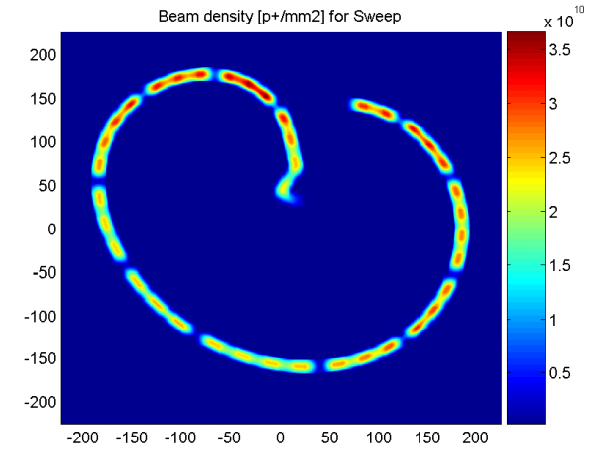
\includegraphics[scale=0.5]{figures/experiment/beamdump.png}
\caption{The trace of a 450 GeV proton beam across the beam dump TDE. The beam structure of bunches and trains is visible along the bath of the sweep. Figure from A Large Diameter Entrance Window for the LHC Beam Dump Line \cite{beamdump}.}
\label{fig:beamdump}
\end{figure}

When the beam has degraded to the point where it is no longer useful, it must be disposed of safely.
Over the course of several hours, the beam loses intensity to the point where it is more efficient to dump the beam and replace it.
Occasionally an error in one of the LHC subsystems will be detected, and the beam is dumped as a precaution.
In both cases, the beam dump system is used to remove the beam from the machine while minimizing damage to its components.

There are three steps in disposing of the beam. 
The first is to extract the beam from its orbit.
The second is to dilute the beam's density.
Finally, the beam is absorbed in a material, where its energy is converted to radiation and heat \cite{lhcDesignV1}.
When an abort is triggered, the procedure depends on the state of the beam.
If the beam is in a safe state, the abort system will wait until the abort gap arrives to ramp up the extraction kicker magnets (MKD).
If the beam needs to be dumped immediately, the MKDs can ramp up outside the abort gap with minimal damage to the system.
The 15 copper wound magnets are powered by a bank of capacitors that can quickly energize the magnets in under 3.0~$\mu s$ to produce a field of 0.34~T. 
Once energized, the MKDs deflect the beam horizontally out of the ring.
The magnets remain on for 90~$\mu s$ to allow the full beam to exit the ring.

Next, the diluter kicker magnets (MKB) sweep out the beam in an ``e'' pattern, as shown in Figure \ref{fig:beamdump}.
This spreads out the area where the beam will deposit its energy.
The diluter is built from four horizontal and six vertical magnets powered by a sinusoidal current to produce the shape.
Like the MKDs, the MKBs are non-superconducting low-oxygen copper wound magnets.

The Extraction Septum Magnets (MSD) have a septum (gap) for the extracted beam.
A low-field hole is drilled through the yoke to allow the passage of the circulating beam.
The MSDs are responsible for deflecting the beam vertically.

Finally, the beam comes to the Beam Dump Absorber Block (TDE).
This consists of carbon cylinders due to its high melting temperature and thermal shock resistance.
In particular, alternating layers of solid polycrystalline graphite cylinders and flexible graphite are used to balance solidity and flexibility.
The total length of the carbon material is 7.7~m long.
The TDE is kept at atmospheric pressure. This raises the question: how is the TDE isolated from the vacuum of the beamline? A low-Z carbon composite layer is used to separate the two, while a thin layer of vacuum insulation prevents small leaks \cite{beamdump}.
The TDE jacket is cooled by water pipes to help reduce the thermal stress on the carbon.
Finally, the assembly is surrounded shielding made from old dipole yokes filled with concrete.

The MKD and MSD magnets used in the beam abort share a design with the magnets used to steer the beam into the rings during injection.
At the beam dump, the MKDs deflect horizontally while the MSDs deflect vertically.
At the injection points, it is reversed, and the MKDs steer the beam horizontally while the MSDs steer it vertically.

\subsection{LHC Operation}

The operation of the LHC is divided into two periods: Run 1 and Run 2.
During Run 1, the physics discovery was made that motivates the search for \vhmm reported in Chapter \ref{sec:hmumu}.
Crucial machine developments were also made in Run 1 that lead to energy and luminosity increases during Run 2, enhancing the precision of the non-resonant search reported in Chapter \ref{sec:ci}.
During Run 2, the machine provided collisions based on the data used for this thesis.
The beam energy reached 6.5~TeV for all proton-proton collisions used in this analysis.
A detailed narrative of the drama and intrigue of both runs is provided in Appendix \ref{sec:appendixLhc}.

\begin{figure}[h!]
\captionsetup[subfigure]{position=b}
\centering
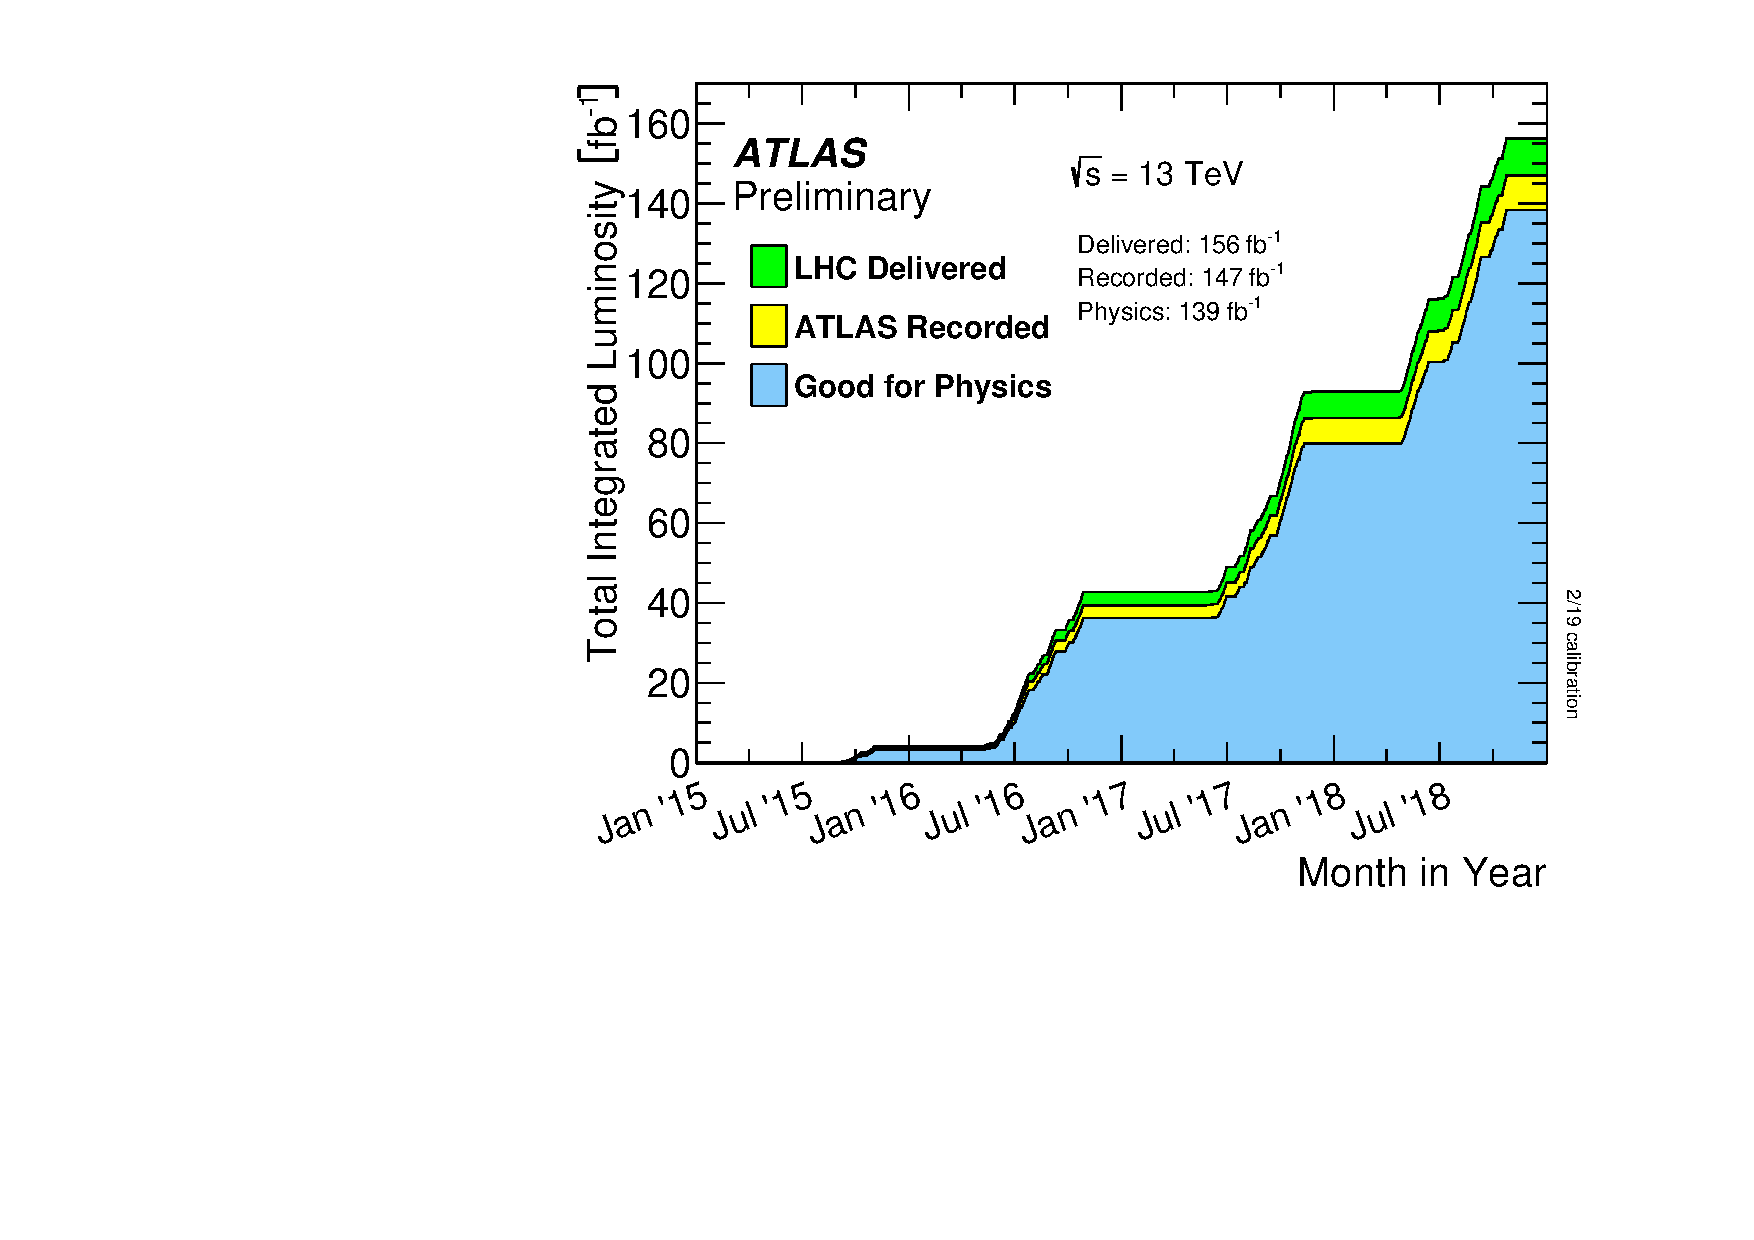
\includegraphics[width=0.75\textwidth]{figures/experiment/lhc/run2Lumi.pdf}
% \caption{ (from: https://twiki.cern.ch/twiki/bin/view/AtlasPublic/LuminosityPublicResults)}
\caption{The total luminosity of $pp$ collisions delivered by the LHC in Run~2, shown in green. The recorded luminosity by ATLAS is shown in yellow, and the portion of this recorded during good operation of the detector is shown in blue  \cite{ATLAS-CONF-2019-021}.}
\label{fig:run2Lumi}
\end{figure}

Run 2 took place during the years from 2015 to 2018.
Each year consists of a period during which the LHC provides collisions to ATLAS and a period during which maintenance and machine research are conducted.
The operation during each year was influenced by the problems of previous years and the solutions and improvements developed to enhance the machine's performance.

Several parameters related to the LHC performance are given in Table \ref{tab:run2}.
The instantaneous luminosity increased over time from $0.5\times10^{34}~\cms$ past the original design target of $1.0\times10^{34}~\cms$ to $2.1\times10^{34}~\cms$.
The general stability of the machine improved and the total number of delivered collisions per year increased.
The number of commissioning days at the start of each year dropped from 58 down to 17, as the LHC was better understood and magnet configurations could be reused from year to year.
These performance improvements were achieved despite a number of persistent challenges to the operation, including magnet short circuits, growing e-clouds, and a mysterious object trapped inside the beam screen.

\begin{table}[htp]
\begin{center}
\caption{Summary of the beam conditions during Run 2 \cite{lhcRun2}.}
{
\begin{tabular}{l r r r r r}\toprule
Parameter & 2015 & 2016 & 2017 & 2018  \\
\midrule
Maximum bunches per beam                 &2244 &2220 &2556 &2556 \\
Emittance ($\mu$m)                       & 3.5 & 2.2 & 2.2 & 1.9 \\
$\beta^*$ (cm)                           & 80  & 40  & 30-40 & 25-30 \\
Total beam energy (MJ)                   & 280 & 270 & 330 & 320  \\
Average stable beam (hours)              & 6.8 & 11.2& 8.2 & 8.3  \\
Delivered integrated luminosity (\fb)    & 4.2 & 38.5 & 50  & 66   \\
Instantaneous luminosity ($10^{34}~\cms$) & 0.5 & 1.4 & 2.1 & 2.1  \\
Average pile-up                          & 13  & 25  & 38  & 37   \\
Stable beam efficiency (\%)              & 35  & 49  & 49  & 49   \\
\bottomrule\end{tabular} %remember cline{1-2}
}
\label{tab:run2}
\end{center}
\end{table}

The performance of the LHC during Run 2 enabled the machine to deliver a total of 156~\fb of collision data.
The total delivered integrated luminosity and that recorded by ATLAS are shown in Figure \ref{fig:run2Lumi}.

\section{ATLAS Detector}

\begin{figure}[h!]
\captionsetup[subfigure]{position=b}
\centering
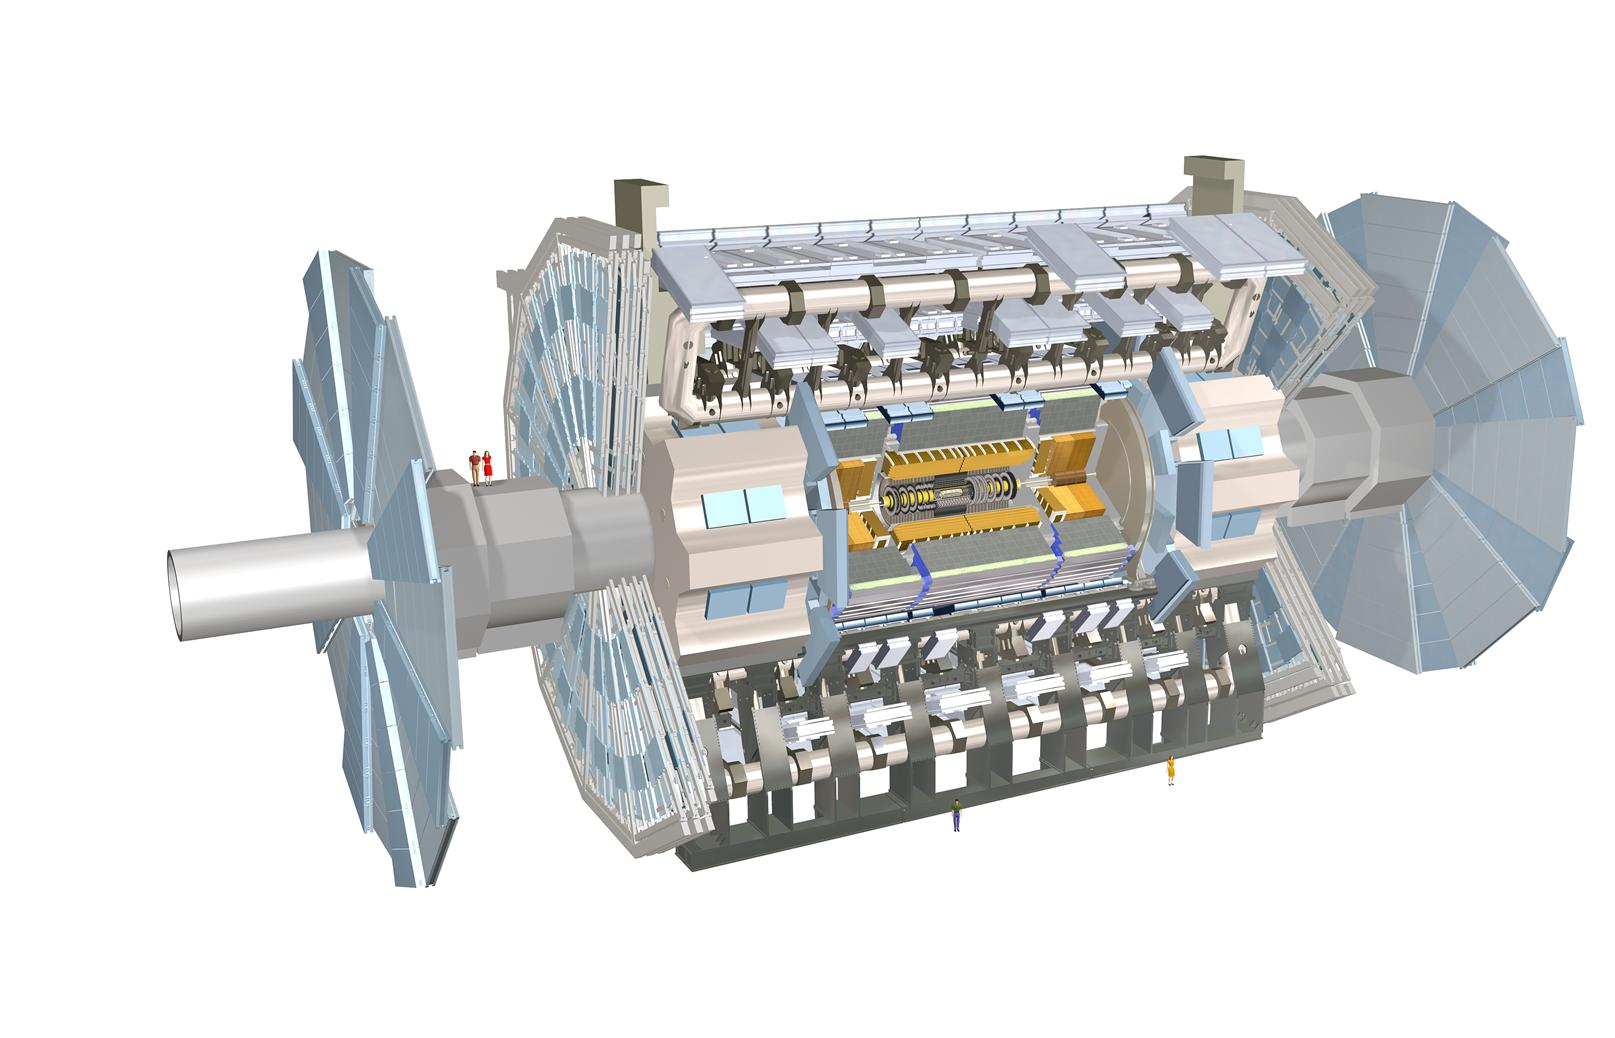
\includegraphics[width=0.75\textwidth]{figures/experiment/atlas/atlasLayout.jpg}
\caption[Computer generated image of ATLAS with a section of the barrel removed for visibility. Illustration by Joao Pequenao.]{Computer generated image of ATLAS with a section of the barrel removed for visibility. Illustration by Joao Pequenao\footnotemark.}
\label{fig:atlas3d}
\end{figure}
\footnotetext{Joao Pequenao. \emph{Computer generated image of the whole ATLAS detector}, 2008. \url{https://cds.cern.ch/record/1095924}}

% \begin{wrapfigure}{r}{0.5\textwidth}
%      \caption[Caption for LOF]{\footnotemark}
%   \begin{center}
%     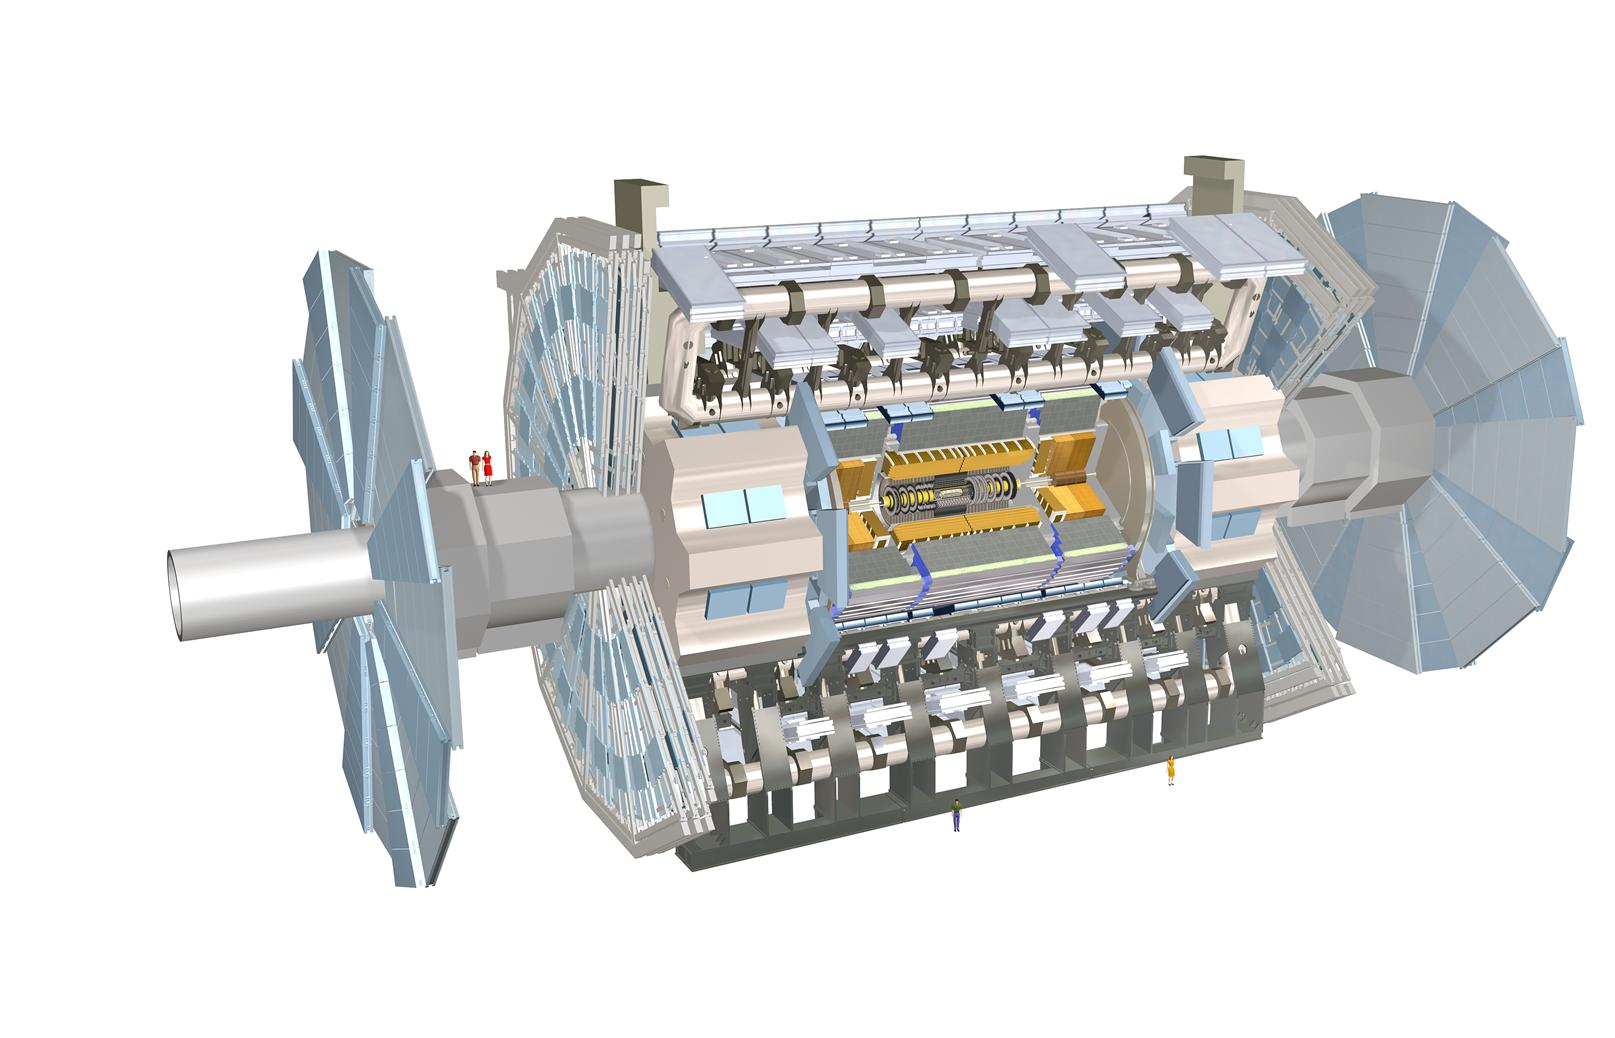
\includegraphics[scale=0.5]{figures/experiment/atlas/atlasLayout.jpg}
%   \end{center}
% \end{wrapfigure}
% \footnotetext{s. 183}

%ATLAS detector
This thesis uses data collected by the ATLAS (A Large Toroidal Lhc ApparatuS) detector.
ATLAS is a multipurpose experiment designed built around an interaction point at the LHC.
Two overarching goals influenced the design of the experiment: to cover as much of the solid angle surrounding the collisions and to precisely measure the particles exiting a collision.
An enormous amount of equipment is required to achieve these goals: the experiment has a cylindrical geometry 46~m in length and 25~m in diameter.

The detector subsystems perform various tasks, ranging from measuring charge tracks left by particles to measuring their energy and momentum.
Some detectors specialize in precisely recording the effects of particles (hits), while others focus on quickly identifying patterns of interest for analysis (triggers).

Throughout the design of the various systems, a key concern is the amount, or budget, of material that each introduces.
Particles may lose energy, be absorbed, or produce secondary particles through interactions as they pass through these materials.
With few exceptions, it is advantageous to reduce the total material that particles pass through.

Four systems comprise the experiment and serve different purposes in the measurement of particles leaving the collisions.
The ATLAS magnet system immerses the detector in a strong magnetic field that bends charged particles proportionally to their momentum.
Three cylindrical coaxial systems interact with both charged and neutral particles to collect information.
The first is the inner detector, which precisely measures the tracks of charged particles.
Next, the calorimeters measure the energies of particles.
Finally, the muon system helps to identify muons and measure their momentum.
The organization of these systems is illustrated in Figure \ref{fig:atlasLayout}.

\afterpage{
\begin{figure}[h!]
\captionsetup[subfigure]{position=b}
\centering
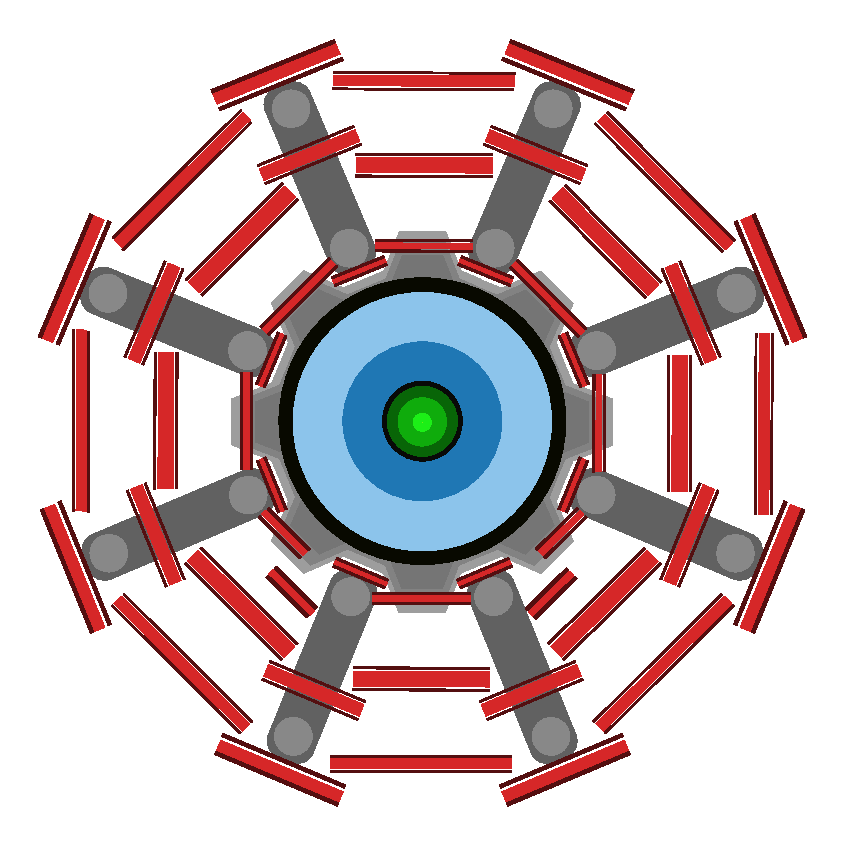
\includegraphics[scale=0.55]{figures/experiment/atlasSide.pdf} \\
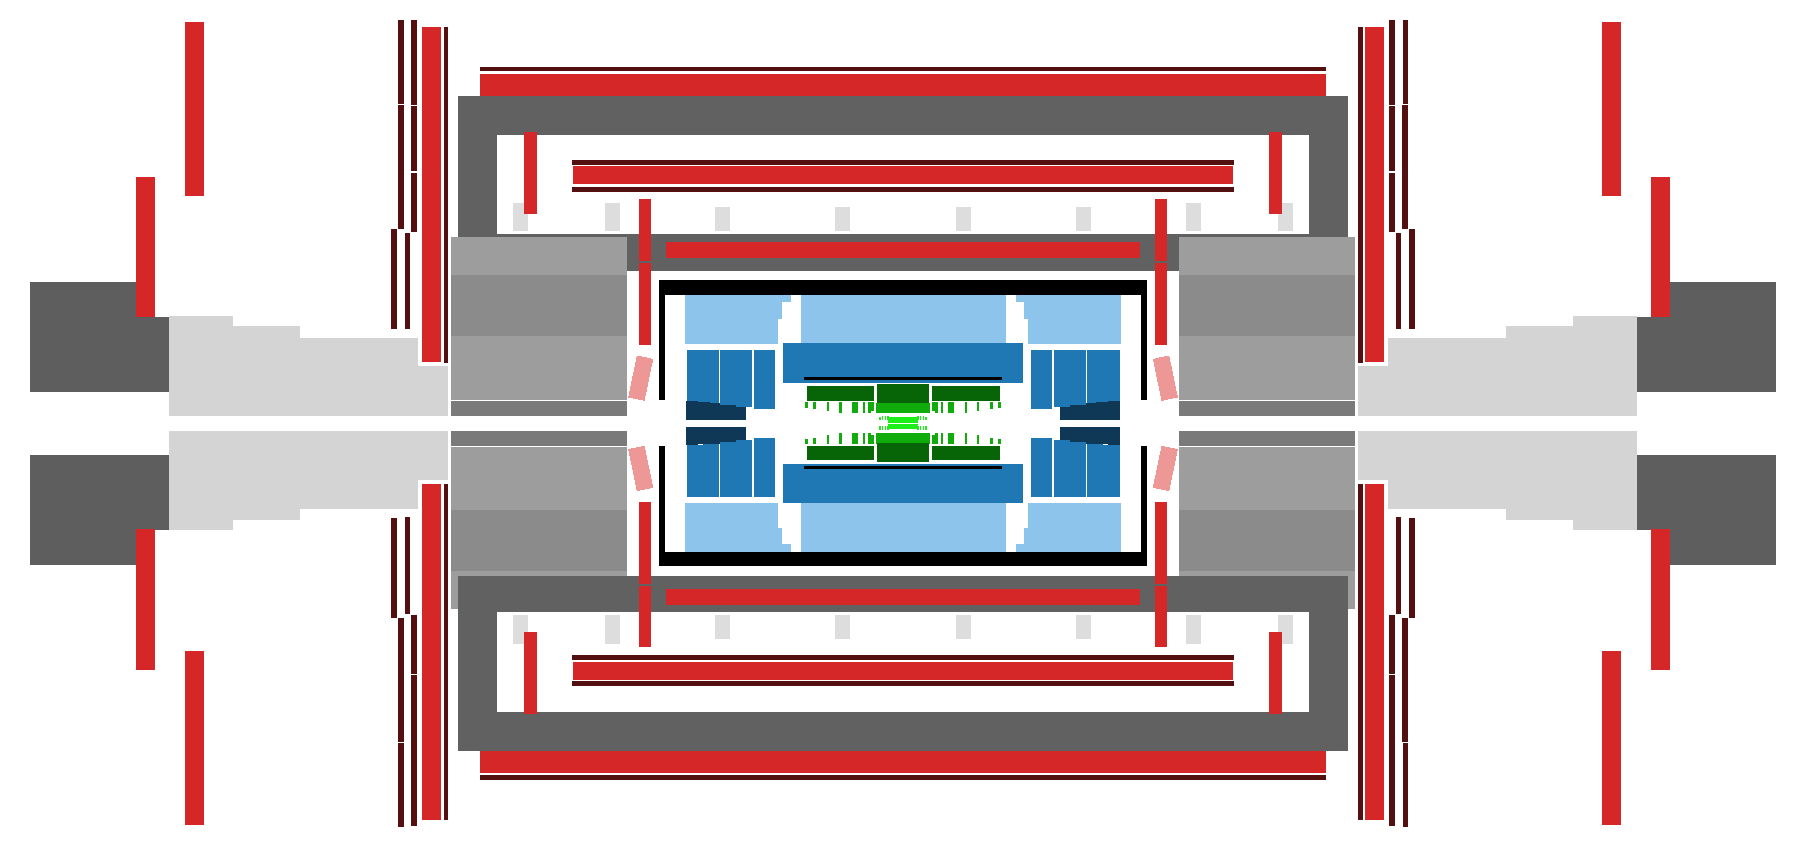
\includegraphics[scale=0.55]{figures/experiment/atlas.pdf}
\caption{Layout of the ATLAS detector with subsystems coded by color. 
\textbf{Top:} a view of the barrel looking along the beamline in the $z$ direction.
\textbf{Bottom:} a view of the detector from the side looking in the $x$ direction.
\textbf{Red:} muon system with CSC (light), MDT (medium), and trigger (dark) chambers. 
\textbf{Blue:} calorimeter system with tile (light), LAr (medium), and FCal (dark) calorimeters. 
\textbf{Green:} inner detector with pixel (light), strip (medium), and TRT (dark) detectors.
\textbf{Grey:} magnet system with ECT (light), BT (medium), and CS (black) magnets.
}
\label{fig:atlasLayout}
\end{figure}
\clearpage
}

% Coordinates
Three coordinate systems are commonly used to describe different aspects of ATLAS and its operation.
A Cartesian coordinate system is defined with its origin at the center of the detector.
The longitudinal $z$ axis runs parallel to the beamline in the counter-clockwise direction when viewed from above.
The $y$ axis points towards the top of the detector, and the $x$ axis points towards the center of the LHC ring.
A cylindrical coordinate system is also defined as sharing the same $z$ axis as the Cartesian system.
The azimuthal angle $\phi$ is defined with respect to the Cartesian $x$ axis, and the radius $\rho$ is defined from the $z$ axis.
Since the detector is nearly symmetric under reversing the $z$ axis, it is helpful to refer to the detector's side with positive $z$ coordinates as the \emph{A side} and the opposite side as the \emph{C side}.
The main body of the experiment, the \emph{Barrel}, is located between the A and C side \emph{end-caps}.
Both of these systems are used in describing the positions of detectors and components within ATLAS.
In particular, the cylindrical system is used to describe the locations of collisions and impact parameter displacements from the beam.

Spherical coordinates are more natural than Cartesian and cylindrical when describing the physical interactions.
This system shares an origin with the previous two systems and shares the azimuthal angle with the cylindrical system.
The radius $r$ is defined from the center of the detector.
The polar angle $\theta$ is defined with respect to the $z$ axis.
It is common to map polar angles onto \emph{pseudorapidity} defined as $\eta\equiv-\ln(\tan\frac{\theta}{2})$.
The pseudorapidity is conveniently calculated from the longitudinal component \plong of a particle's total momentum $p$ as $\eta=\arctan{\frac{\plong}{|p|}}$.

% Particle ID
While detectors in ATLAS measure the location of, and energy deposited by, particles, it is the arrangement of detectors that allows the experiment to identify the particle type.
Electrons, photons, muons, and other particles interact differently with various layers of the detector.
Certain idiosyncratic patterns are compatible with different particle types.
For example, charged particles leave tracks of energy deposited in the inner detector, while neutral particles pass directly through.
Electrons are stopped with a shower of electromagnetic radiation in first calorimeter, while muons penetrate out to the muon spectrometer.
Examples of these patterns are shown in Figure \ref{fig:particleInteractions}.
The various patterns left by different particles are evident.
A charged hadron bends in the magnetic field, leaving a curved track in the inner detector, before depositing its energy in the outer hadronic calorimeter.
A neutral hadron leaves no track before producing a hadronic shower.
Electrons are similarly differentiated from photons by their track in the inner detector as well as the shape of their electromagnetic showers in the inner calorimeter.
The direction that particles bend helps determine their electric charge, while the radius of their curved track helps determine their momentum.

\begin{figure}[htb]
\captionsetup[subfigure]{position=b}
\centering
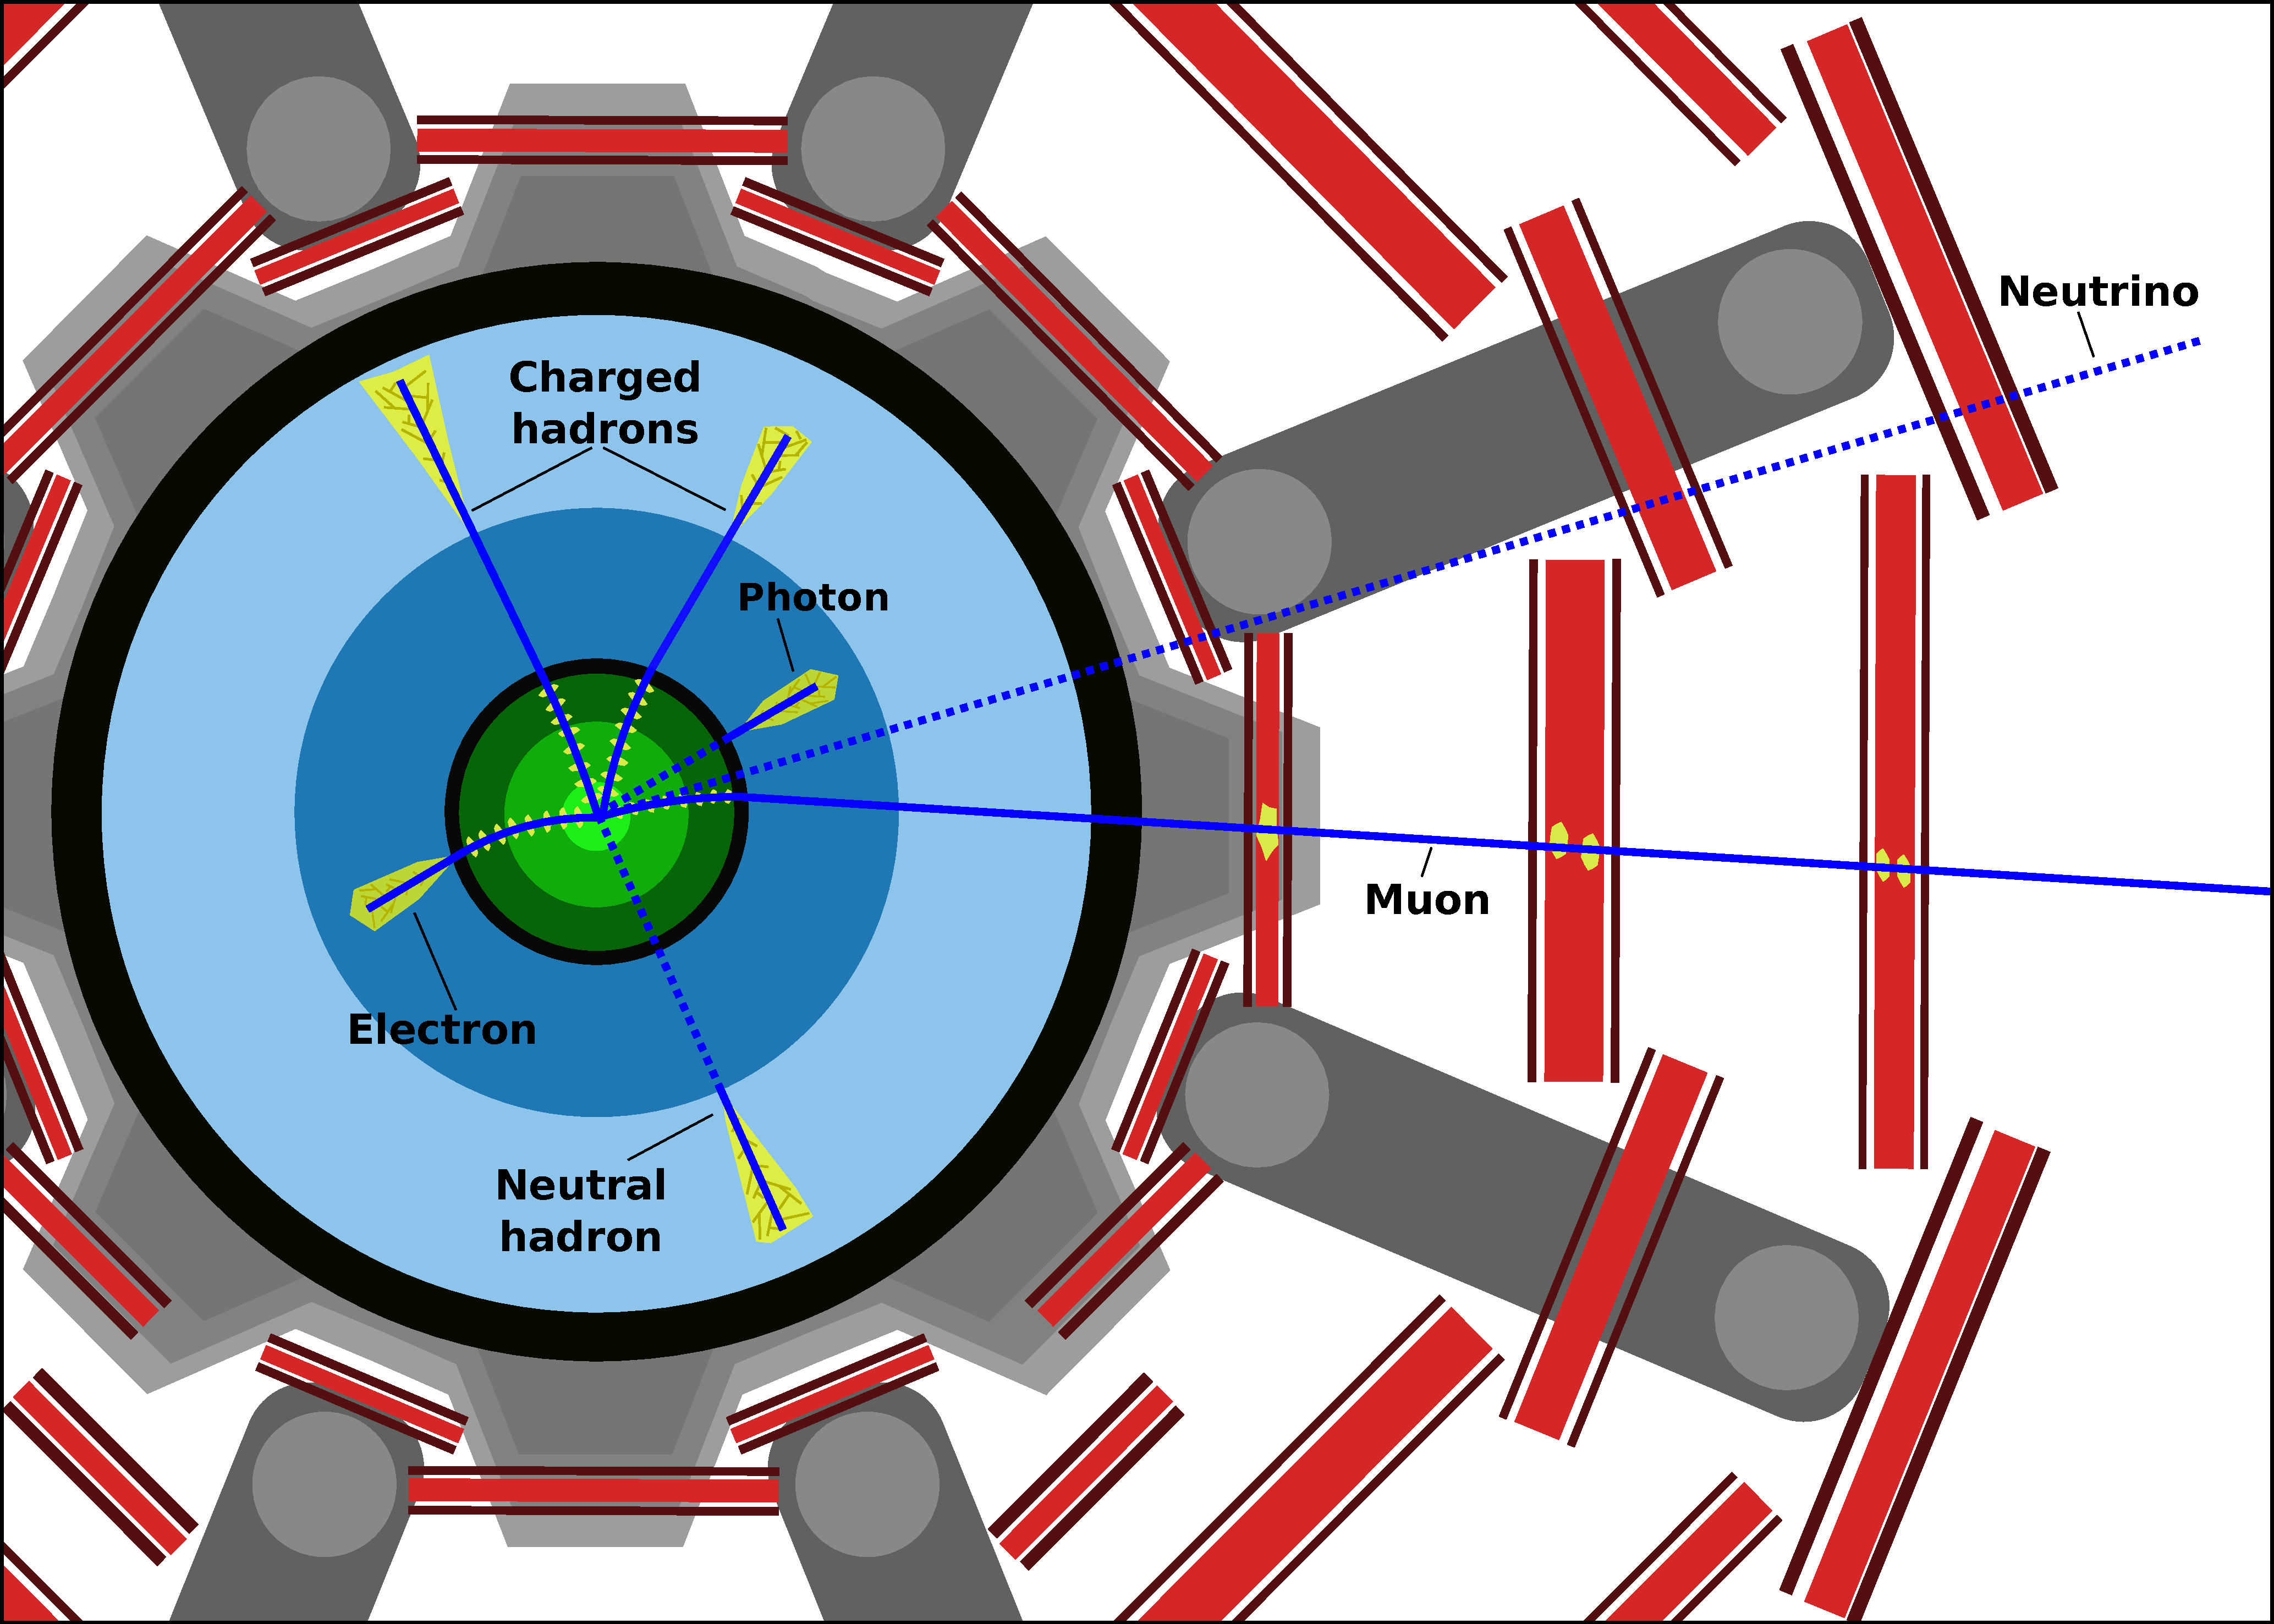
\includegraphics[width=0.95\textwidth]{figures/experiment/particleId.pdf}
\caption{A cross section of ATLAS looking along the beamline. The detectors are color coded: green for the inner detector, blue for the calorimeter, and red for the muon spectrometer. Several particle paths are shown in blue. Dashed lines represent a particle passing through the detectors without interacting. Yellow areas indicate electromagnetic or hadronic showers in the calorimeters and other interactions with the detector. Outside the inner solenoid, the muon is bent parallel to the beamline by a toroidal magnetic field.}
\label{fig:particleInteractions}
\end{figure}

This section will describe the experiment's design, beginning with the four systems that make up the ATLAS.
Following this, the systems for identifying interesting collisions and recording them will be presented.




\subsection{Inner Detector}

\begin{figure}[h!]
\captionsetup[subfigure]{position=b}
\centering
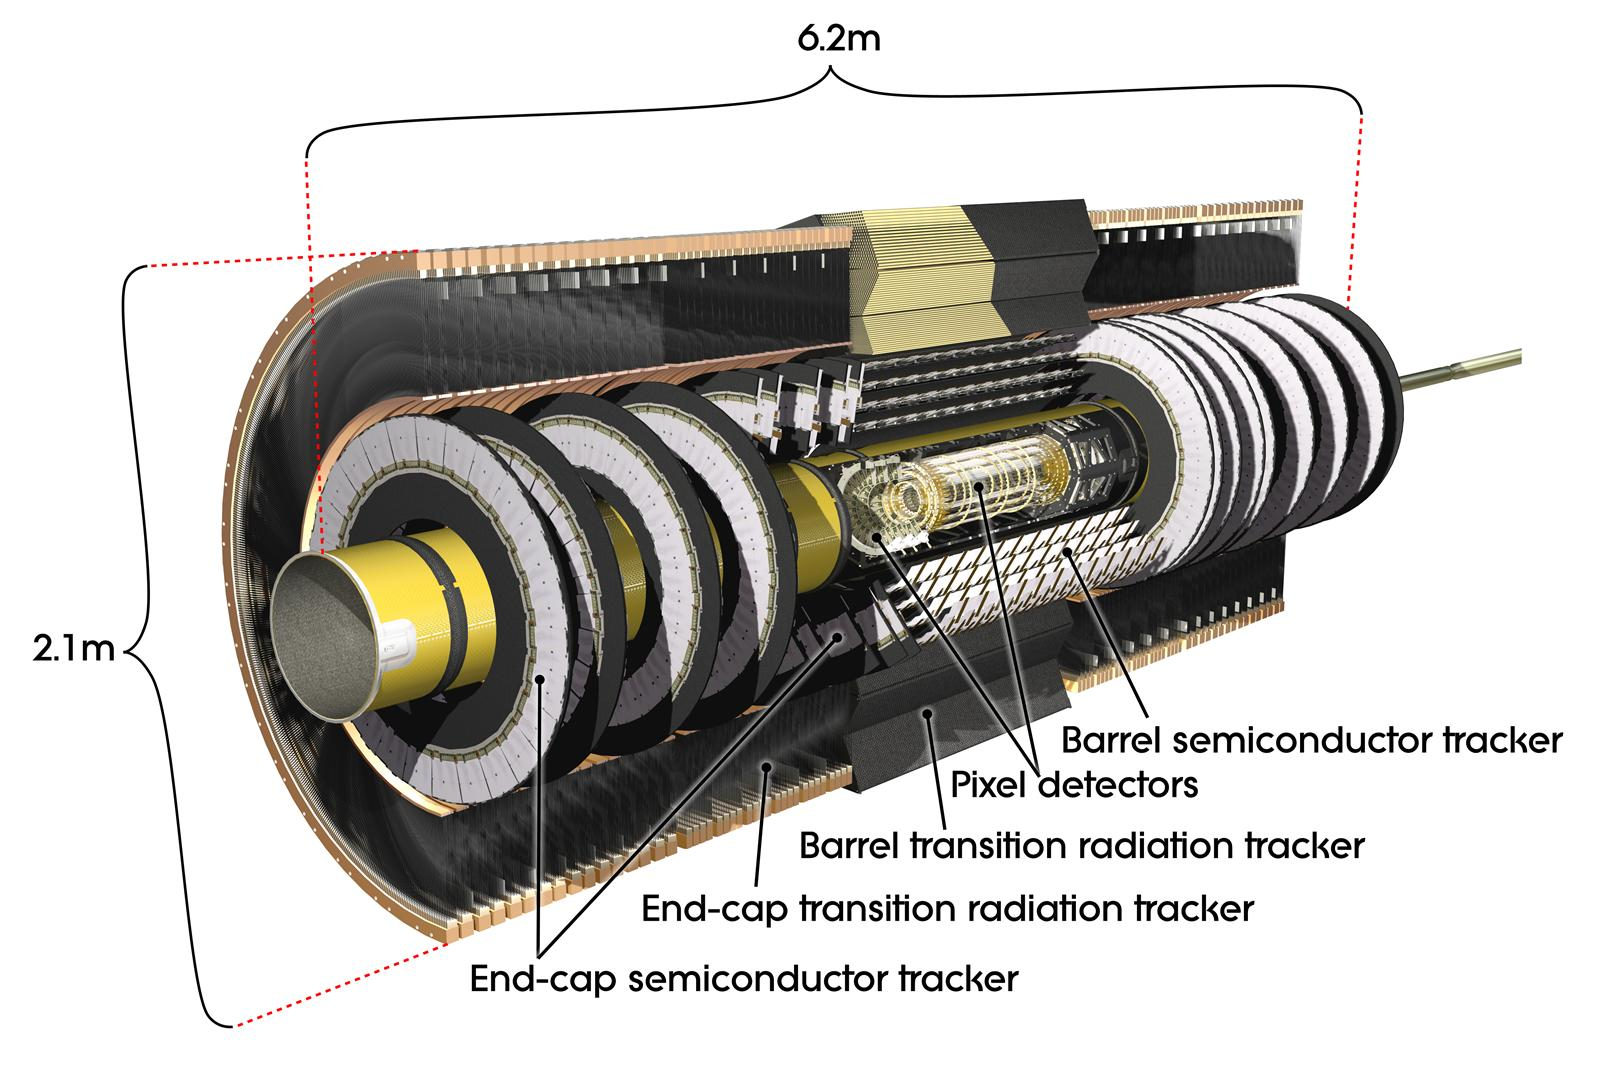
\includegraphics[width=0.8\textwidth]{figures/experiment/atlas/id.jpg}
\caption[Computer generated image of the inner detector with a section removed for visibility. Illustration by Joao Pequenao.]{Computer generated image of the inner detector with a section removed for visibility. Illustration by Joao Pequenao\footnotemark.}
\label{fig:atlasId}
\end{figure}
\footnotetext{Joao Pequenao. \emph{Computer generated image of the ATLAS inner detector}, 2008. \url{https://cds.cern.ch/record/1095926}}

The ATLAS Inner Detector (ID) is the innermost detector system.
Its purpose is to precisely measure the locations of energy deposits left by particles leaving a collision.
To this end, it is comprised of three subsystems: the pixel detector, the silicon-strip tracker, and the transition radiation tracker.
These are shown in Figure \ref{fig:atlasId}.
These are positioned in coaxial cylindrical arrangements around the region of the beam pipe where collisions take place.
The cylinders arrange detectors in a barrel covering $|\eta|<1$ and bookended by two mirrored end-caps.
The total length of the ID is 7~m and the diameter is 2.3~m, which enables the full coverage of $|\eta|<2.5$.
The data from the ID subsystems (hits) are used to identify tracks left by particles as they transverse the detector.
In this regard, it helps measure the impact parameter of particles with a precision that enables the identification of decay products of bottom quarks and tau leptons that travel short distances before decaying\cite{pixel}.


Both the pixel detector and the silicon-strip tracker belong to the category of solid-state silicon detectors in that they detect ionizing particles through their interaction with a semiconductor.
These use a semiconductor layer doped with an element with an electron affinity (p-type) and a semiconductor layer doped with an electron donor element (n-type).
At the interface between these two layers, electrons equilibrate from the n-type material to the p-type material, producing a \emph{depletion region} and an electric field.
A positive voltage bias is applied to the n-type side of the juncture to expand the depletion region and strengthen the field.
When a charged particle passes through the depletion region, it ionizes atoms and liberates electron-hole pairs.
Under the influence of the electric field, these drift to either end of the depletion region and produce a measurable current.
Drift does not occur outside the depletion region in the absence of an electric field \cite{grupen}.

The first subsystem that particles pass through is the pixel detector.
Here, the silicon is subdivided into a grid of many isolated \emph{pixels} that may be read out individually.
Each pixel is 256~\um thick with a typical surface area of $\sim50\times400\um^2$.
In the barrel, these are grouped into arrays of 24$\times$160 pixels for readout.
Sixteen arrays are located on a ``module'', which serves as the repeating basis of the various pixel layers.
Four layers of detectors are arranged in the barrel, with the inner most layer located inside the beampipe, with radii of 2.9~cm, 5.1~cm, 8.9~cm, and 12.3~cm. 
In each end-caps, four disks are arranged between $z$=11~cm and $z$=20~cm \cite{pixel,pixel2}.
The next subsystem that particles interact with is the silicon-strip tracker (SCT).
The SCT barrel consists of four cylindrical layers, while the end-caps each consist of nine disk layers.
Each barrel layer is built from modules that host two layers of silicon wafers divided into lines of microstrips that are 126~mm long.
The strips are oriented differently in the barrel depending on their layer, with some running parallel to the beam axes and others offset at an angle of 40~mrad \cite{sct}.

Finally, particles interact with the transition radiation tracker (TRT) positioned outside the SCT.
This is a system of 4~mm diameter gaseous proportional-mode drift tubes.
The tubes, or ``straws'', are made from wound Kapton with a gold-plated 31~\um wire in the center.
The straws are filled with a drift gas mixture of xenon (70\%), carbon dioxide (27\%), and oxygen (3\$).
During operation, the Kapton is kept at a -1.5~kV.
When a charged particle passes through a straw, it ionizes the gas and the resulting free electrons drift towards the grounded wire.
The induced current is amplified and read out by front end electronics.
The space between the straws is filled with polymer and foil materials so that charged relativistic particles produce transition radiation when they pass through material interfaces.
This is strongest for electrons ($\propto E/m$) and is useful for their identification against pions.
The TRT complements the silicon detectors by providing a large number of tracking points while adding very little to the material budget.
As a result, the 73 layers of tubes are used in the barrel, while 160 layers make up the end-caps.
A charged particle passing through the barrel will produce hits in $\sim30$ TRT straws.
Additionally, the fast readout rate of 80-100~kHz compensates for the relatively slow readout possible with the silicon detectors  \cite{trt}.

In total, 1.5$\times10^{8}$ data channels are read out from the ID, with the majority of these coming from the pixel detector.
The ID is used to measure tracks left by muons and electrons, to identify displaced vertices from b-jet decays, and measure to overall momentum expelled from collisions.

\subsection{Calorimeters}

\begin{figure}[h!]
\captionsetup[subfigure]{position=b}
\centering
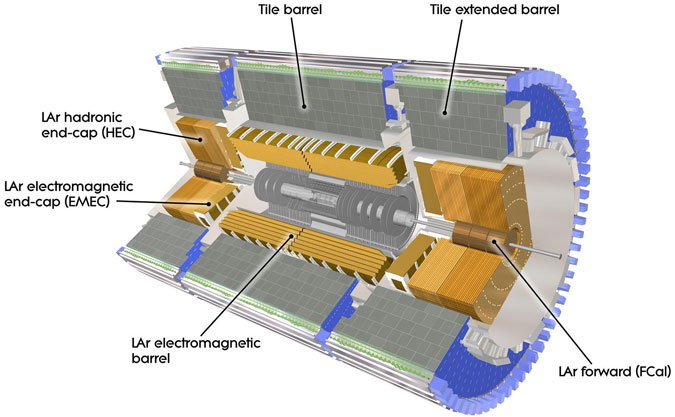
\includegraphics[width=0.7\textwidth]{figures/experiment/atlas/calo.jpg}
\caption[Computer generated image of the calorimeters with a section of the removed for visibility. Illustration by Joao Pequenao. ]{Computer generated image of the calorimeters with a section of the removed for visibility. Illustration by Joao Pequenao\footnotemark. }
\label{fig:atlasCalo}
\end{figure}
\footnotetext{Joao Pequenao. \emph{Computer Generated image of the ATLAS calorimeter}, 2008. \url{https://cds.cern.ch/record/1095927}}

The ATLAS Calorimeter System is comprised of two subsystems: the Liquid Argon Calorimeter (LAr), the Tile Calorimeter.
The LAr is designed to measure energy deposited through electromagnetic interactions.
The Forward Calorimeter is part of the LAr and is positioned in the large-$\eta$ region and provides additional calorimeter coverage.
Wrapped around the exterior of LAr, the Tile Calorimeter is designed to measure the energies of hadronic jets.
Together, these make up the calorimetry system shown in Figure \ref{fig:atlasCalo}.
This is particularly useful in determining the energies of photons and electrons, and to a lesser extent, muons.

The calorimeters in ATLAS are divided into electromagnetic and hadronic types.
The electromagnetic calorimeters measure the energy lost by electrons through bremsstrahlung radiation and the energy lost by photons through electron-positron pair production.
Both processes occur at a rate related to the thickness of material they travel through in terms of \emph{radiation length} $X_0$.
\footnote{$X_0\equiv\frac{A}{4\alpha N_AZ^2r_e^2\ln(183Z^{-1/3})}$, where $Z$ and $A$ are the atomic number and weight, $r_e\equiv\frac{1}{4\pi\epsilon_0}\frac{e^2}{m_ec^2}$ is the classical electron radius, $N_A$ is Avogadro's number, and $\alpha$ is the familiar fine structure constant.}
Electrons with energy $E$ loose their energy while traveling through a material per length $x$ at a rate:
\begin{equation}\begin{split}
    -\frac{dE}{dx}=\frac{E}{X_0}.
\end{split}\end{equation}
Photons undergo pair production with a probability based on their frequency:
\begin{equation}\begin{split}
    -\frac{dw}{dx}=\frac{1}{\lambda_\text{pair}}e^{-x/\lambda_\text{pair}}; \quad \lambda_\text{pair}=\frac{9}{7}X_0.
\end{split}\end{equation}
Both processes produce secondary electrons and photons that in turn produce their own showers of lower energy particles.
If the radiation length of the material is enough, most of the initial particle's energy will be deposited in the material.
This energy can be converted into scintillation light or into the ionization of an \emph{active} material, both of which may be used for detection  \cite{grupen}.

Hadronic calorimeters work along with similar principles to electromagnetic calorimeters, except the primary interactions are nuclear instead of electromagnetic.
They measure the energy of hadrons, which is particularly useful at ATLAS to measure the energy of columnated jets of hadrons produced by collisions.
The radiation length is replaced with the average nuclear interaction length $\lambda_I\approx35\text{g/cm}^2A^{1/3}$, where $A$ is the atomic mass number.
The instead of pair production and bremsstrahlung, hadrons traveling through a calorimeter lose their energy through momentum exchanged through nuclear interactions.
This results in a \emph{cascade} of light hadrons and, to the detriment of all of physics, neutrinos produced from the initial incoming hadron.
These can be distinguished from an electromagnetic shower by their broad width that begins deeper within the calorimeter.
The charged products of the cascade can produce detectable scintillation light that may be used for detection  \cite{grupen}.


For homogeneous calorimeters such as those in ATLAS, the energy measured in the shower can be used to estimate the energy of the original particle.
This is limited by several uncertainties: the point of the first interaction, leakage of the shower out through the calorimeter.
The measurement of energy by the calorimeters is specified by a resolution of the form in Equation \ref{eqn:caloRes}.
\begin{equation}\begin{split}\label{eqn:caloRes}
    \frac{\Delta E}{E}=\frac{\sigma_a}{\sqrt{E}}\oplus\frac{\sigma_b}{E}\oplus\sigma_c.
\end{split}\end{equation}
Here, the term $\sigma_a$ is a stochastic uncertainty in photoelectric statistics.
The term $\sigma_b$ has a value of $\approx0$ at ATLAS.
The term of constant relative uncertainty, $\sigma_c$, is due to uncertainty in the calibration.
For high-energy events, the constant term dominates.

\subsubsection{Liquid Argon Calorimeter}

\begin{figure}[h!]
\captionsetup[subfigure]{position=b}
\centering
\subfloat[][]{\label{fig:atlasTile}{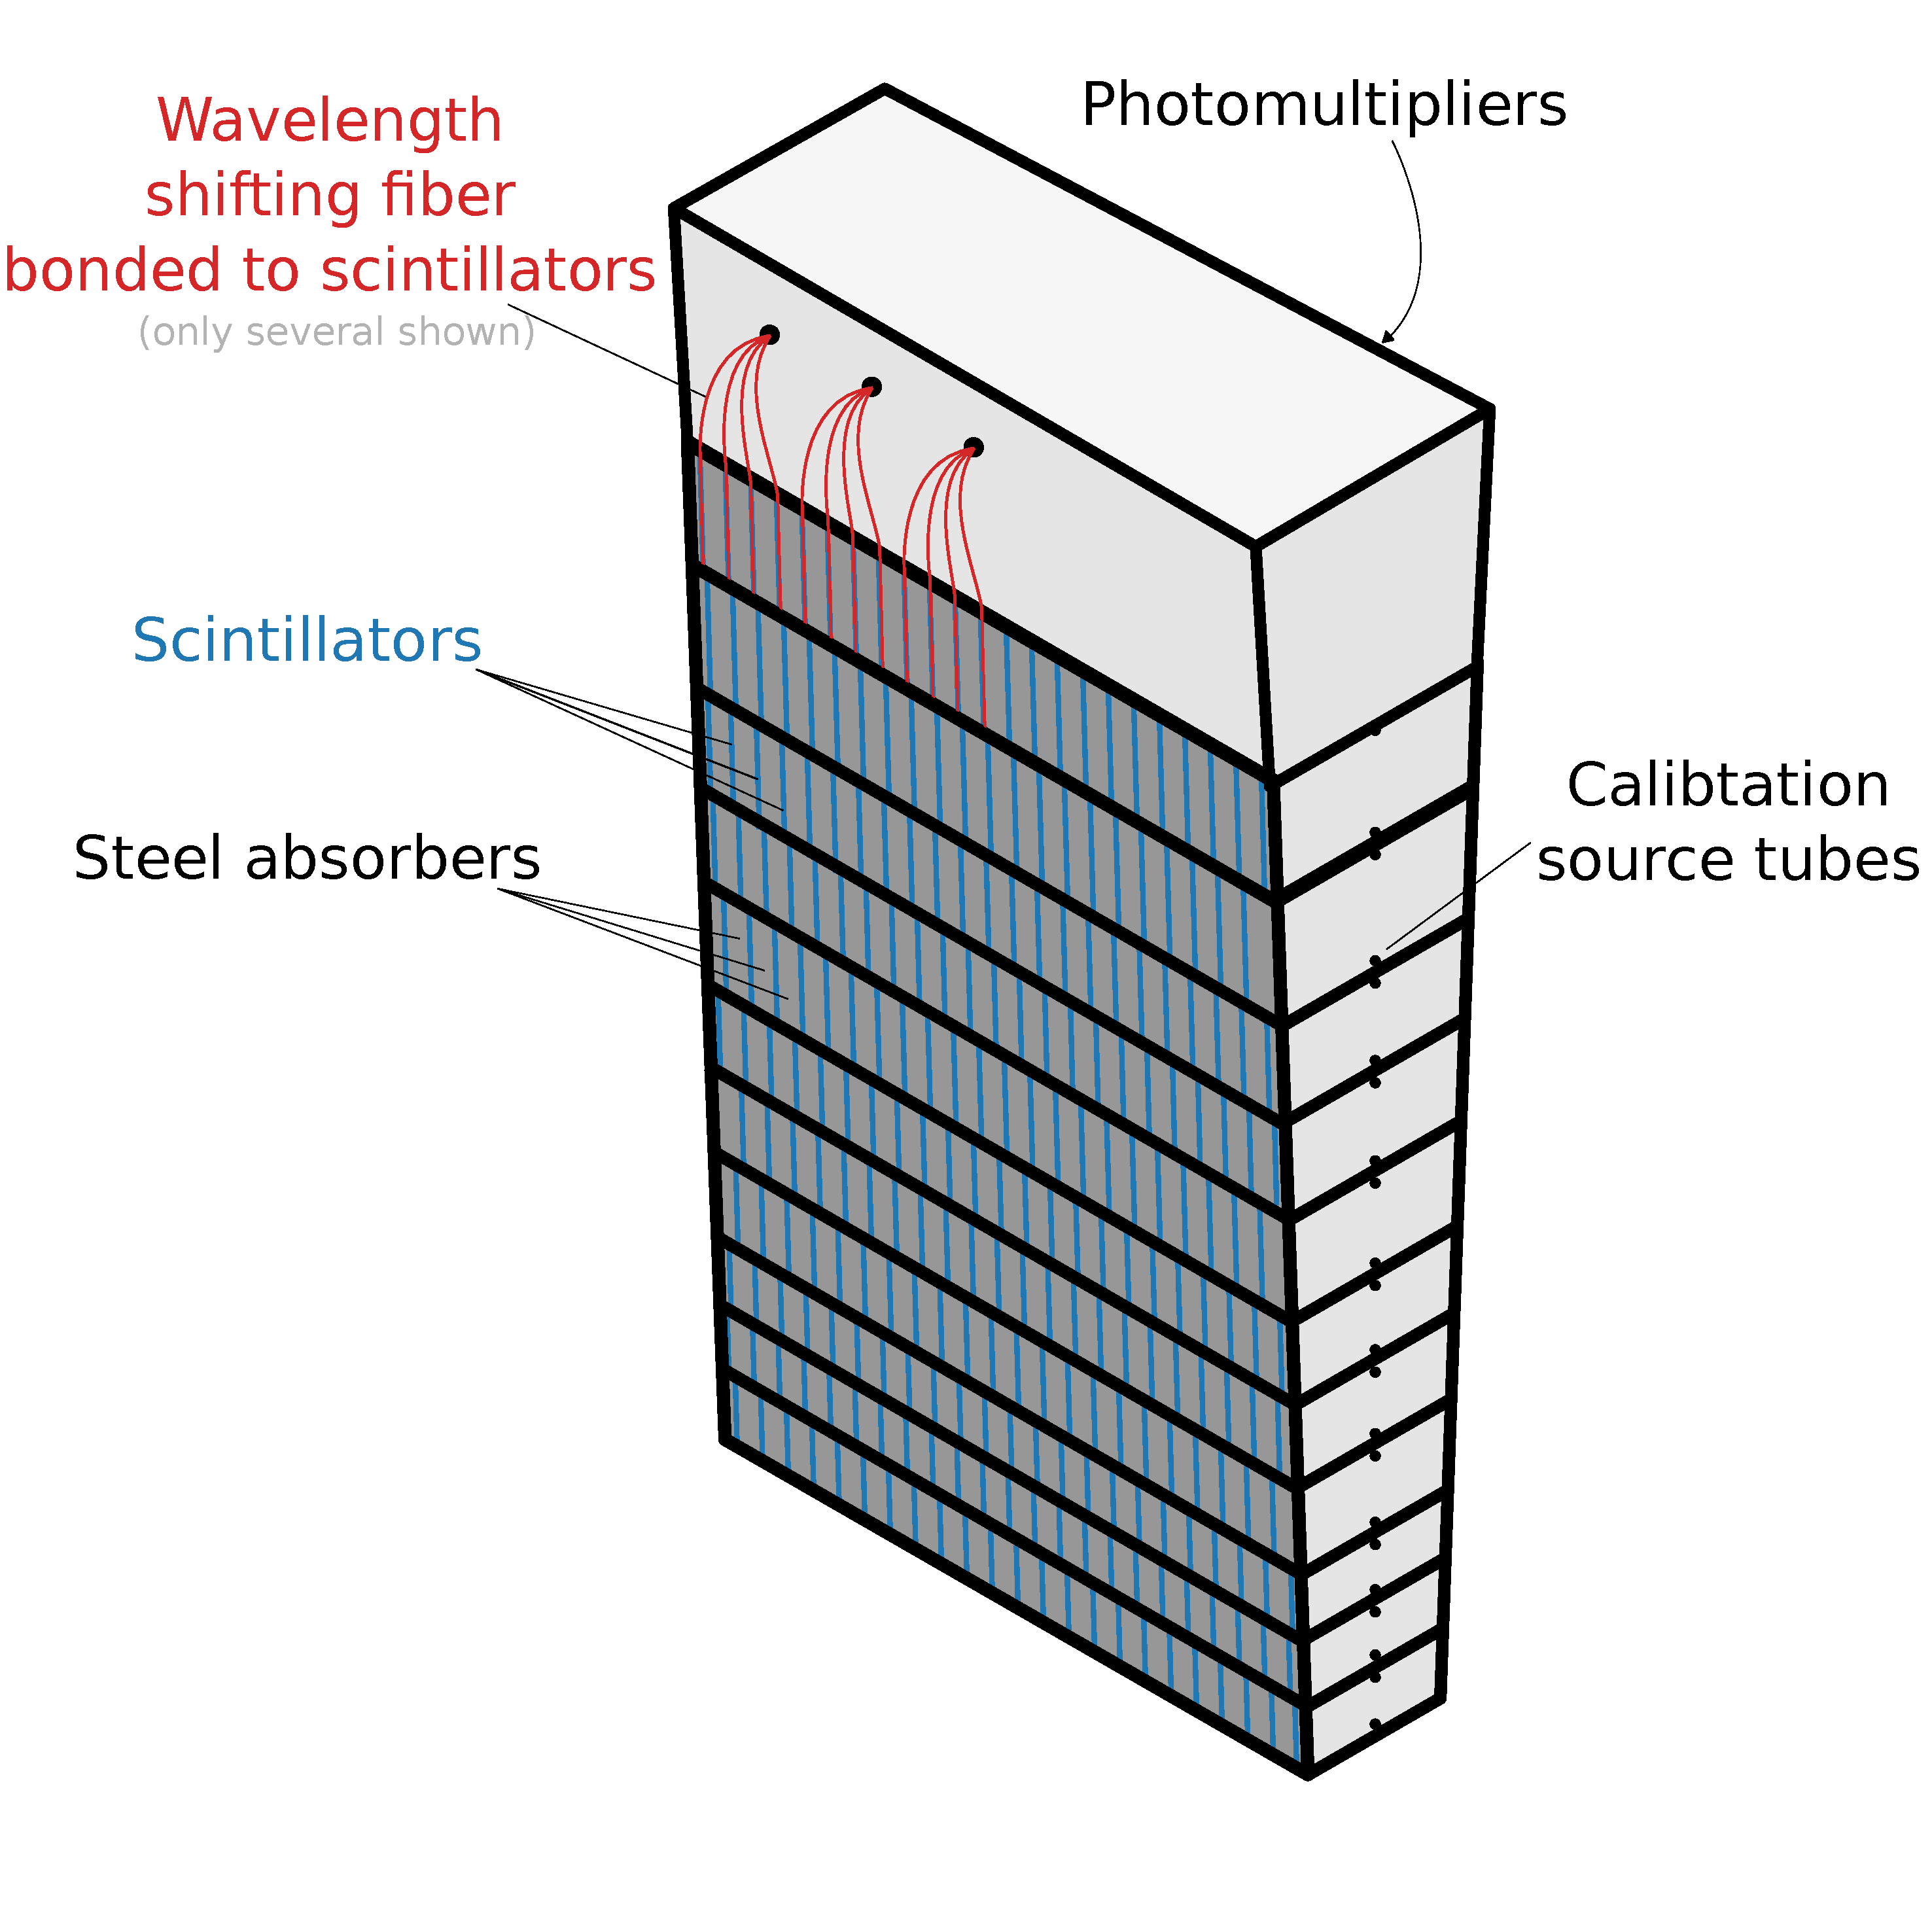
\includegraphics[width=0.50\textwidth]{figures/experiment/atlas/tile.pdf}}}
% \subfloat[][]{\label{fig:atlasTile}{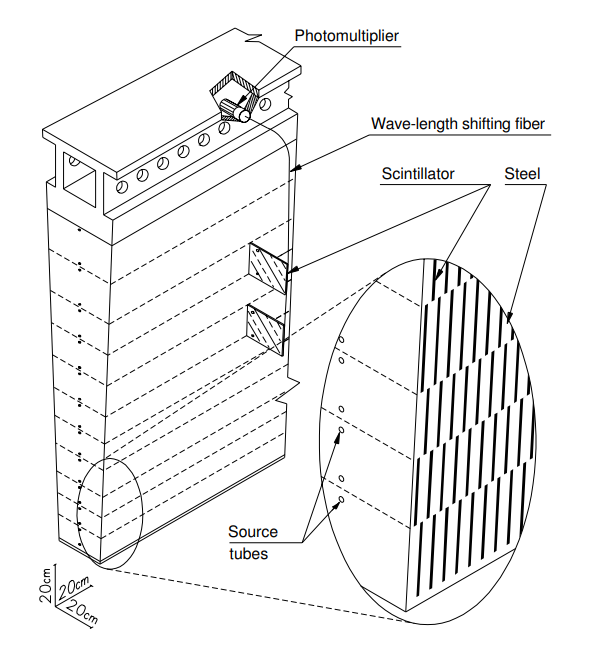
\includegraphics[width=0.40\textwidth]{figures/experiment/atlas/tile.png}}}
\subfloat[][]{\label{fig:atlasLar}{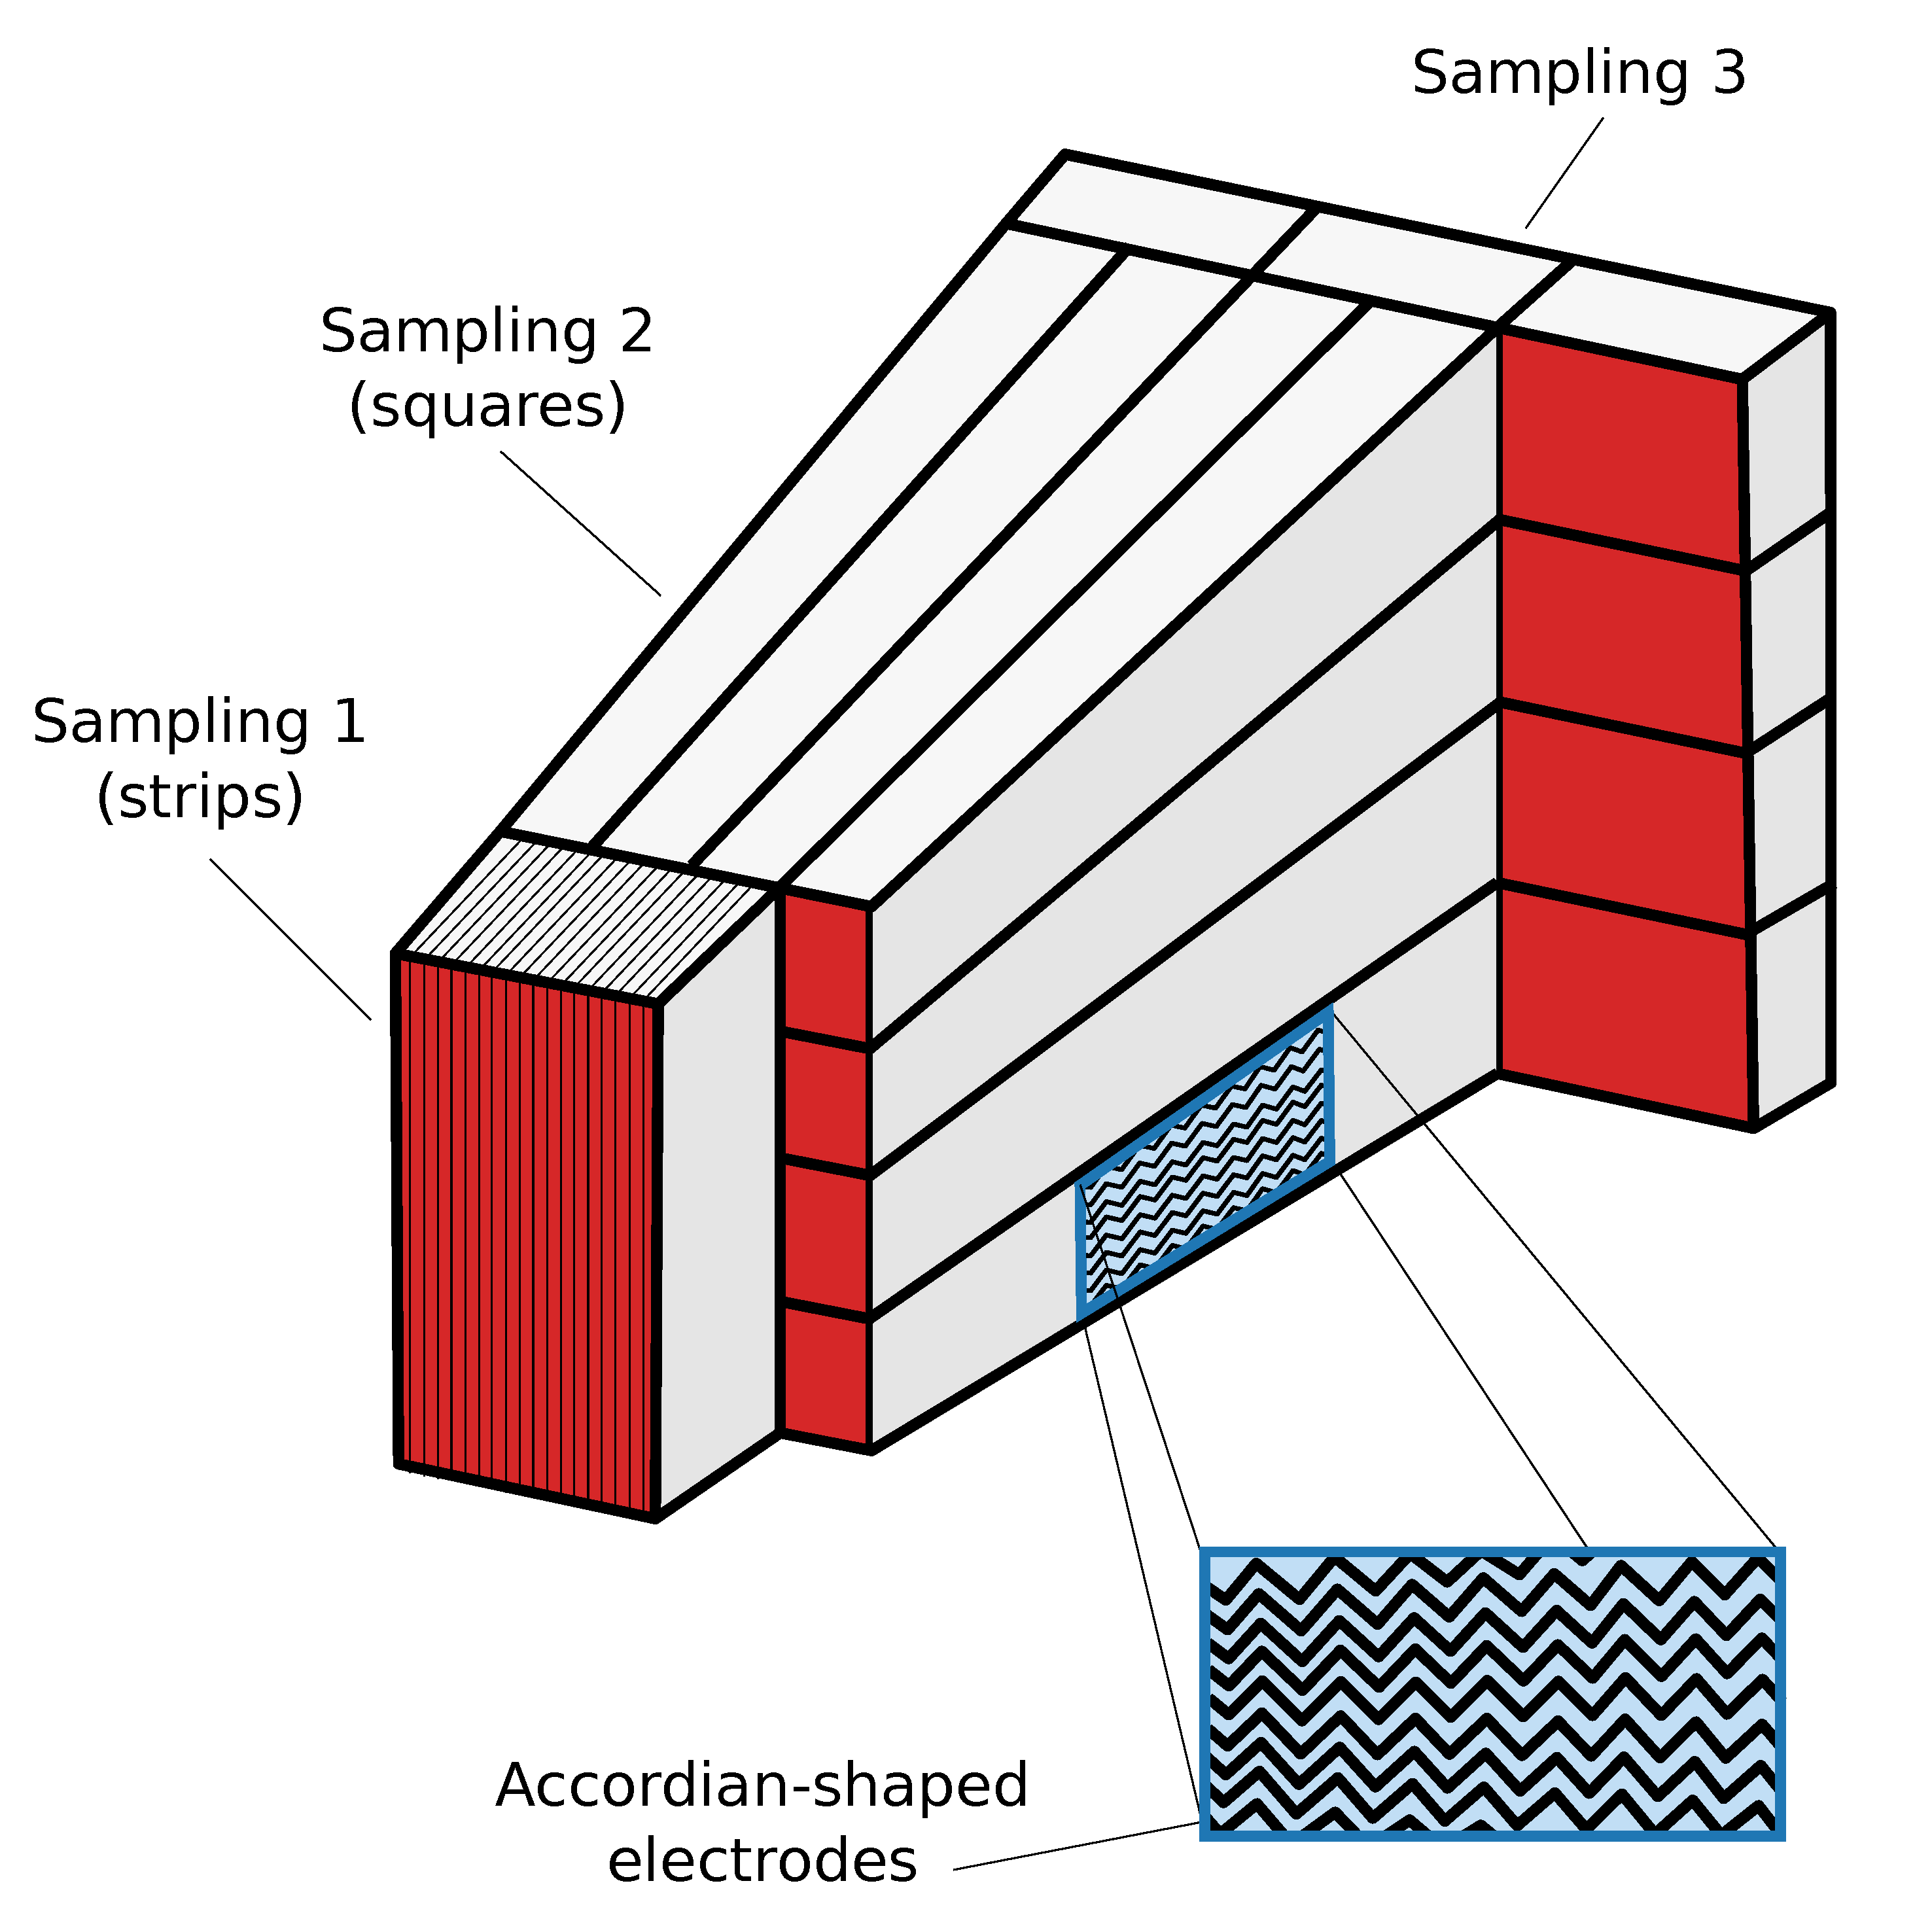
\includegraphics[width=0.50\textwidth]{figures/experiment/atlas/lar.pdf}}}
% \subfloat[][]{\label{fig:atlasLar}{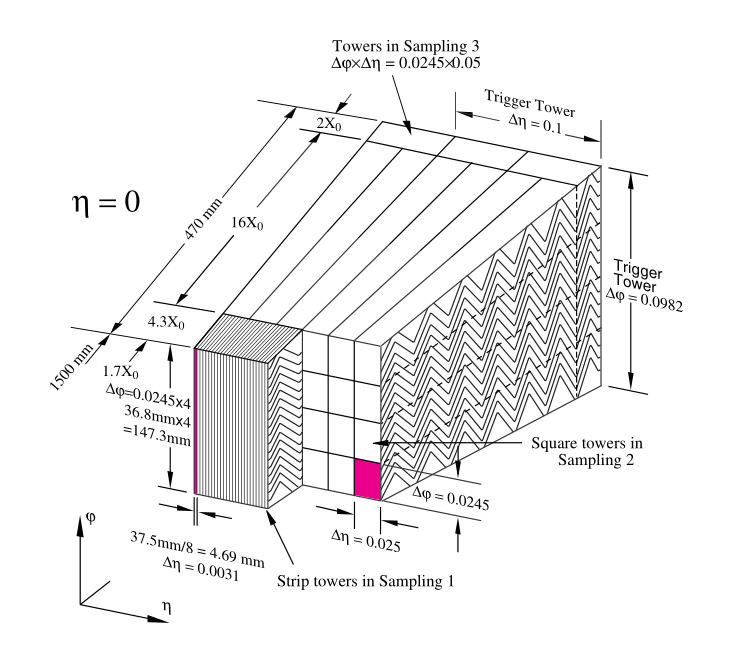
\includegraphics[width=0.60\textwidth]{figures/experiment/atlas/lar.png}}}
\caption{(a) A module in the TileCal consisting of staggered scintillator (blue) and steel (grey) layers read out on both sides by fiber optics connected to photomultipliers. Source tubes in the TileCal allow radioactive sources to be inserted for calibration. (b) A section from the LAr, consisting of towers (red) composed of accordion shaped electrodes submerged in liquid argon.}
\label{fig:atlasCalo}
\end{figure}

The Liquid Argon Calorimeter is situated outside of the inner detector.
It is divided into subsystems for the barrel region and end-cap regions.
The barrel consists of two symmetric half-cylinder electromagnetic calorimeters.
In the end-cap regions, the LAr electromagnetic end-cap (EMEC) is followed by the LAr hadronic end-cap (HEC) and then the Forward Calorimeter (FCal).
The electromagnetic calorimeters cover $|\eta|<3.2$.
The combined coverage with the HEC and FCal covers $|\eta|<4.8$

The primary purpose of the barrel and EMEC calorimeters is to measure the energy of photons and electrons.
Both systems share a similar construction.
Accordion shaped electrodes made of copper etchings on polyimide substrates are held at a voltage of 2~kV.
Between the electrodes, grounded steel-clad lead absorbers interact with primary incident particles and produce showers of electrons and photons.
Both the electrodes and the absorbers are submerged in cryogenic liquid argon that acts as the active material.
The primary and secondary particles ionize the argon, which produces showers of electrons that drift towards the electrodes.
The electrodes are organized into narrow strip towers, square sampling towers, and wide trigger towers.
Signals are read out from individual towers.
These are illustrated in Figure \ref{fig:atlasLar}.
A particle passes through a series of towers in the calorimeter.
The first are the strip towers, which form a presampler that helps correct for the amount of energy lost before reaching the calorimeter.
After the presampler, a particle enters the sampling towers.
With a radiation length of approximately $X_0=20$, these are longer than the presampler and consequently absorb the majority of the energy from electron or photon showers.
Finally, the shower reaches the trigger towers on the outer layer of the LAr.
The total radiation length in the barrel is over $X_0=22$.
The design of the barrel and EMEC calorimeters provides a relative energy resolution $\sigma_a=10\%$ and $\sigma_c=0.7\%$  \cite{lar}.

The HEC wheels consist of alternate copper absorbers and electrodes.
The electrodes have the same design as those from the electromagnetic calorimeters but are flat instead of accordion-shaped.
The radiation length of the HEC is $X_0=10$.
This design provides a resolution with $\sigma_a=50\%$ and $\sigma_c=3\%$.
The FCal is located within the HEC at a higher $\eta$.
It has a very different geometry, consisting of a copper layer followed by two tungsten layers.
These are perforated by circular holes, in which slightly smaller rods are inserted.
The gap between the layer and the rod serves as the drift volume.
The FCal design measures energies to a resolution with $\sigma_a=100\%$ and $\sigma_c=10\%$  \cite{lar}.

\subsubsection{Tile Calorimeter}

The ATLAS Tile Calorimeter (TileCal) is built surrounding the LAr calorimeters and designed to measure the energies of hadronic jets.
Its relative position is illustrated in Figure \ref{fig:atlasCalo}.
It makes use of sheets of steel as the absorbing material and scintillating plates as the active material.
The TileCal consists of three barrel segments and, unlike the previously discussed detectors, no end-cap components.
The central barrel is 5.6~m long, while the two outer ``extended'' barrels are 2.9~m long.
The barrels have an inner radius of 2.3~m and an outer radius of 4.2~m.
The central barrel covers a pseudorapidity of $|\eta|<1$ and the extended barrels provide coverage up to $|\eta|<1.7$.
The energy resolution of the Tile design is $\sigma_a=50\%$ and $\sigma_c=7\%$  \cite{tileTdr}.

As a hadronic calorimeter, the operating principle of the TileCal is similar to the LAr calorimeters.
Each module of the TileCal consists of stacks of absorber and scintillator tiles, as shown in Figure \ref{fig:atlasTile}.
These are staggered in radial layers and perpendicular to the beamline.
Incident hadrons interact with the absorbers and produce hadronic cascades.
These, in turn, scintillate as they pass through the 3~mm plastic scintillator tiles.
Two fiber optic cables collect scintillation light from each tile, transform its wavelength, and carry it to a bank of photomultiplier tubes, where it is digitized.
The effective hadronic depth of the TileCal is $\sim7\lambda_I$  \cite{tile}.

\subsection{Muon System}

\begin{figure}[h!]
\captionsetup[subfigure]{position=b}
\centering
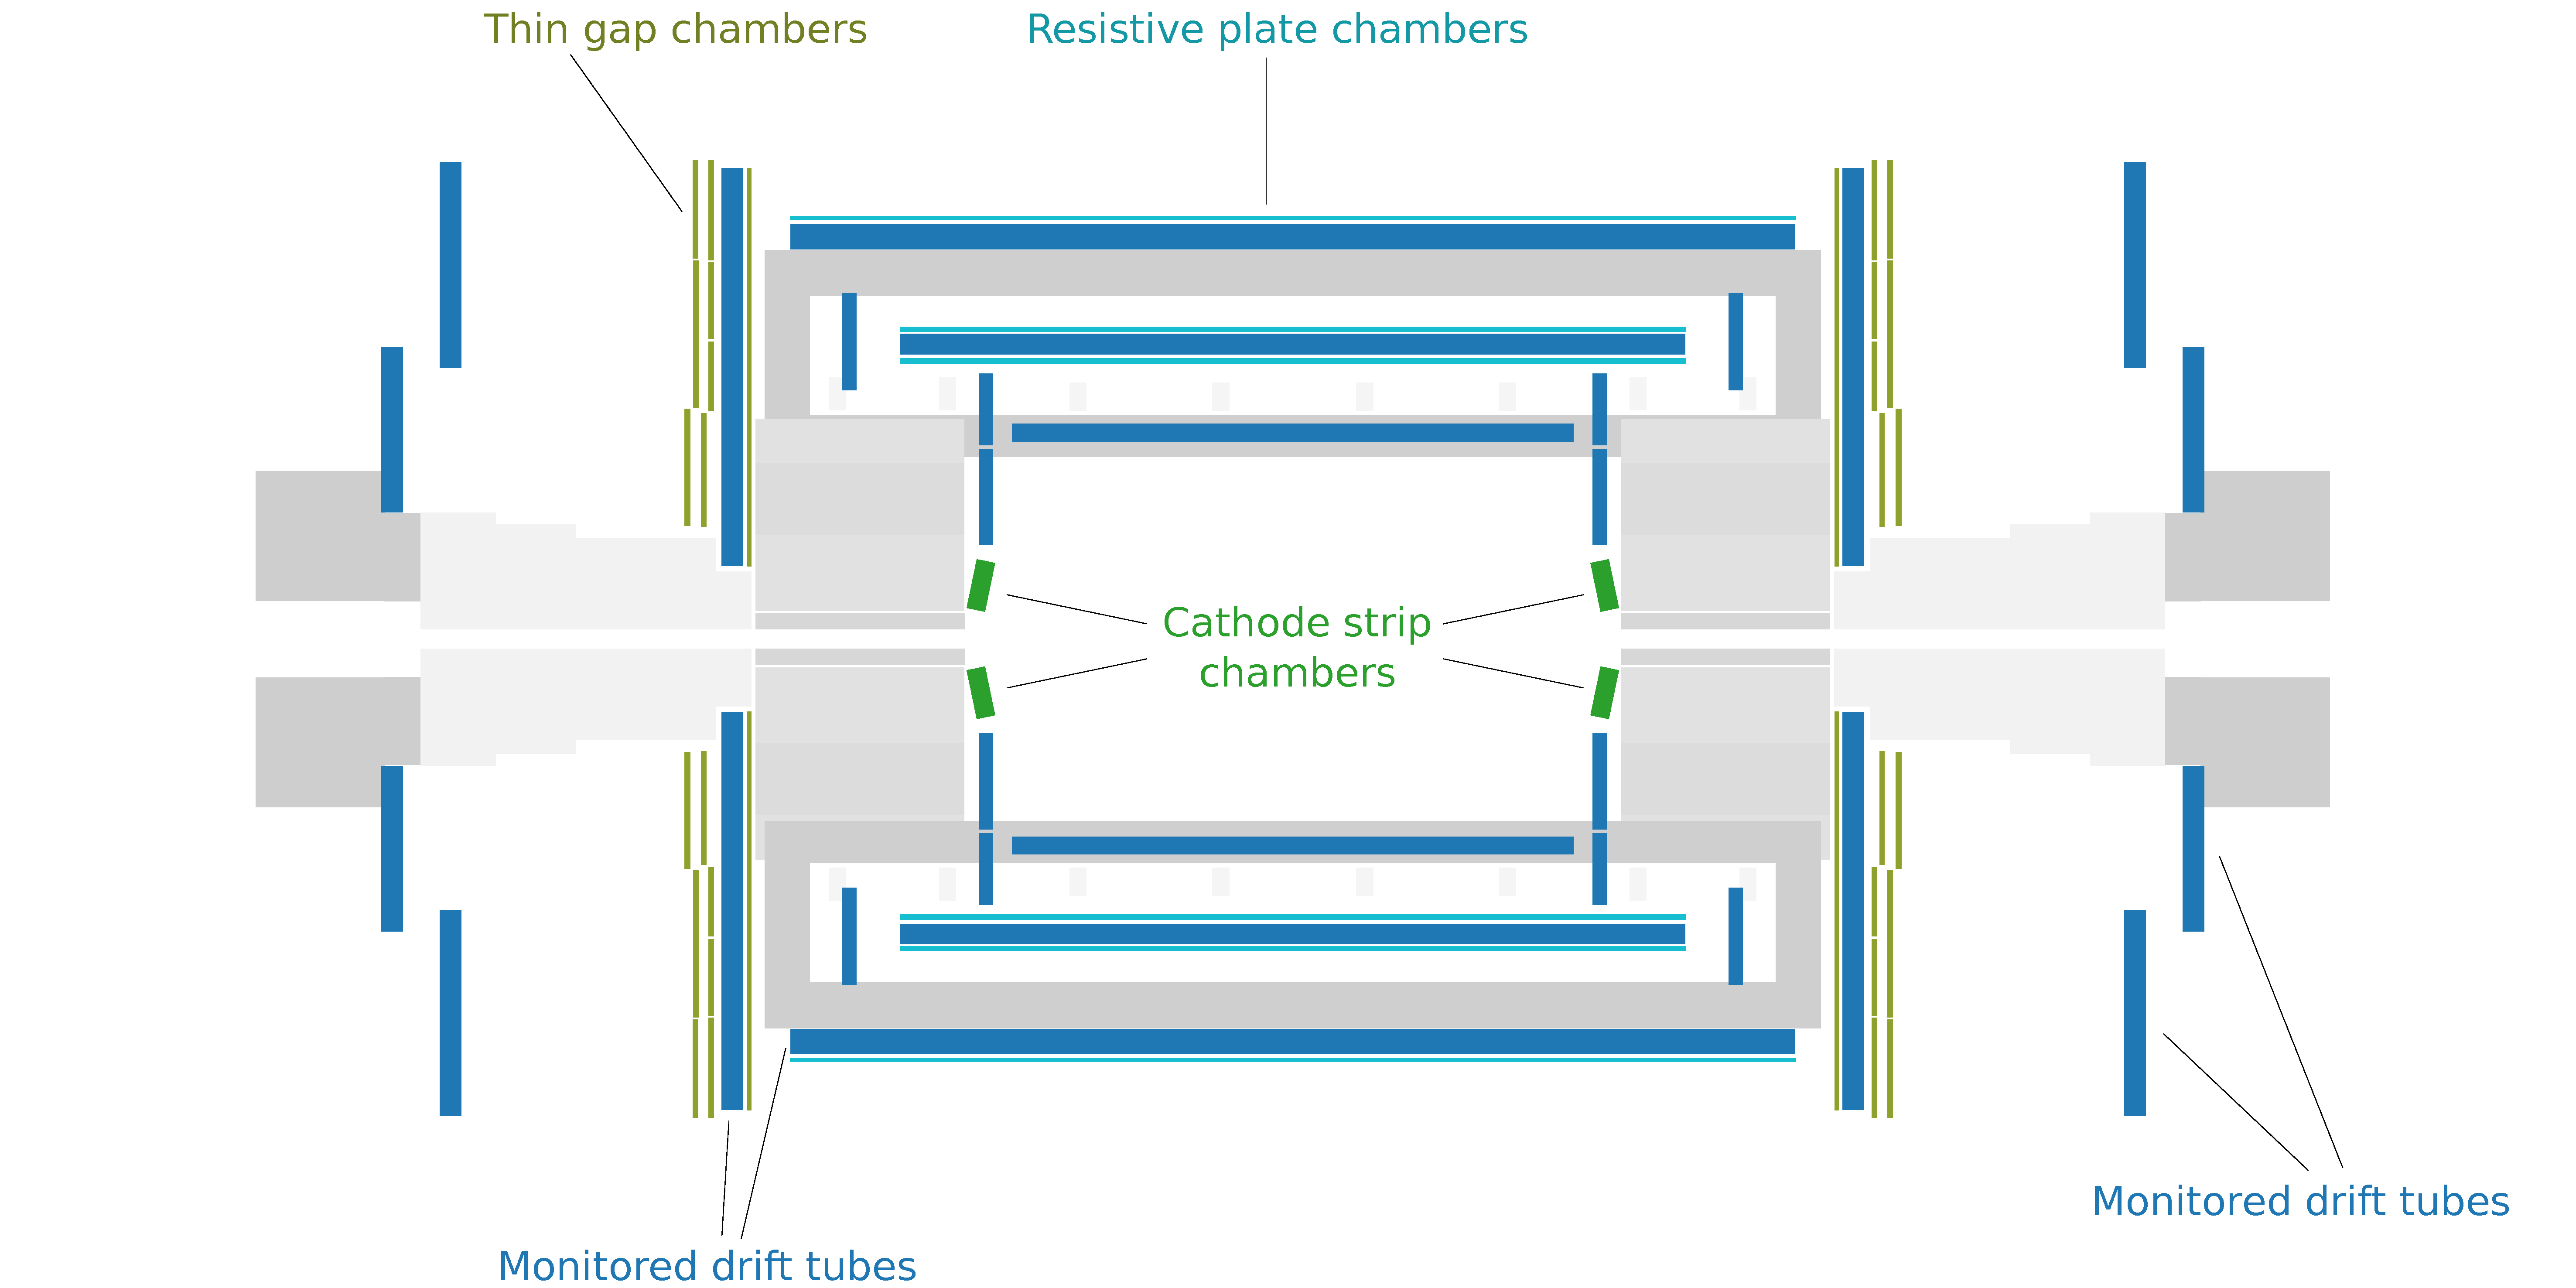
\includegraphics[width=0.8\textwidth]{figures/experiment/muonSys.pdf}
% 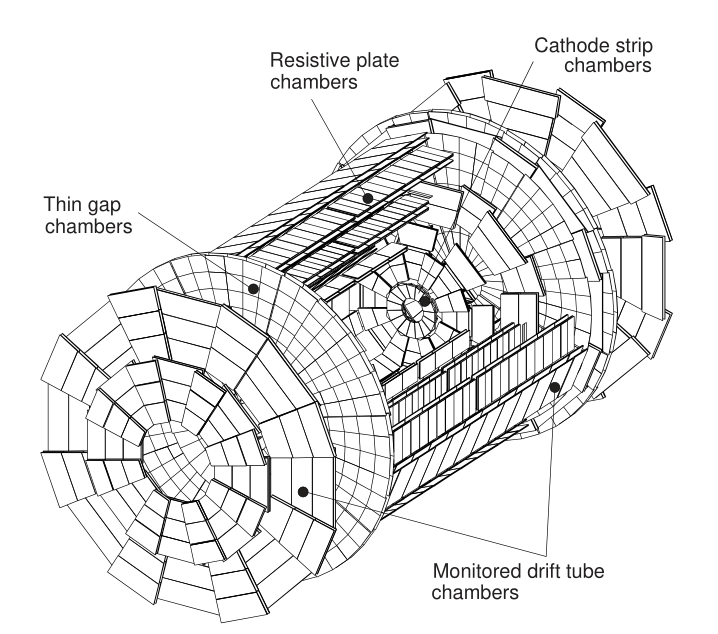
\includegraphics[width=0.8\textwidth]{figures/experiment/atlas/muon.png}
% \subfloat[][]{\label{fig:atlasMsBarrel}{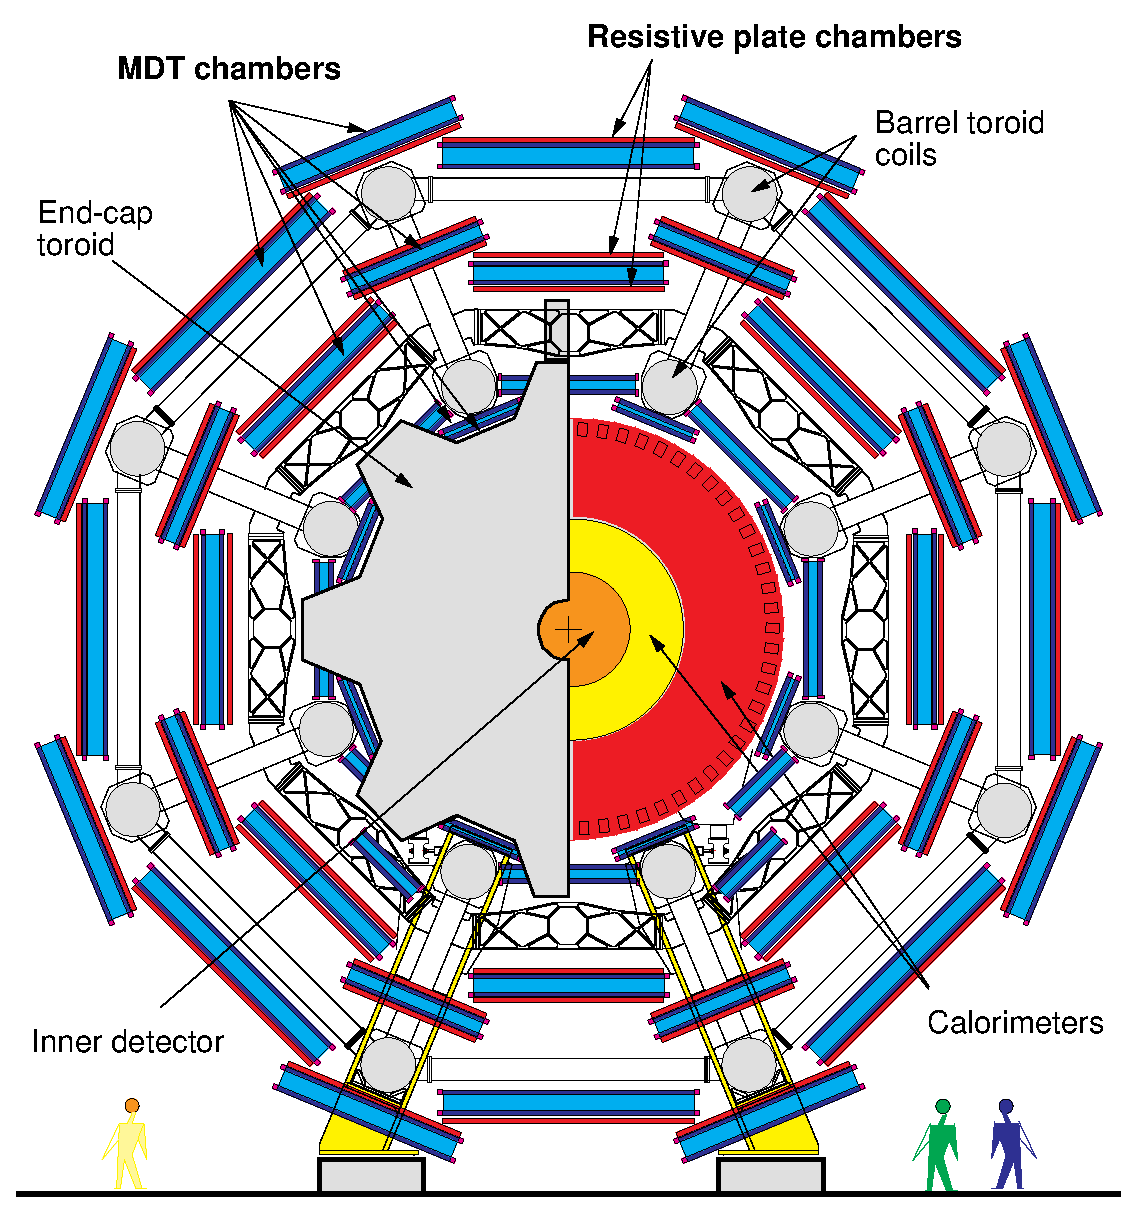
\includegraphics[width=0.5\textwidth]{figures/experiment/atlas/muonCross.eps}}}
\caption{ATLAS muon system, with chambers of various types labeled.}
\label{fig:atlasMs}
\end{figure}

The outermost detector system, the ATLAS Muon Spectrometer (MS), is the largest muon spectrometer ever constructed.
The MS can identify muons and measure their transverse momentum, especially for those with $\pt>300$~GeV.
In this task, it shares a similar geometry to the ID.
The spectrometer is comprised of a barrel region with cylindrical layers of detectors at radii of 5, 7.5, and 10~m.
The symmetrical end-cap regions consist of four layers located at $z$ of 7, 10, 14, 21-23~m.
All layers have 16-fold symmetry in azimuth.
The MS uses four subsystems in different regions of pseudorapidity and for different tasks.
To provide fast hits to the trigger system in order to identify events containing muons, the Resistive Plate Chambers operate in the barrel ($|\eta|<1.05$), and the Thin Gap Chambers operate in the end-cap wheel ($1.05<|\eta|<2.7$).
Precision tracking data for muons is provided by the Monitored Drift Rubes in the barrel ($|\eta|<2.7$) along with the Cathode Strip Chambers in the region from $2.0<|\eta|<2.7$.
The various systems are shown in Figure \ref{fig:atlasMs}  \cite{muonTdr}.

The function of the MS is to measure transverse momentum using a track of hits left by a muon as it bends in a strong magnetic field.
The hits directly determine the sagitta $s$ of the track, which is related to the angle of magnetic deflection $\theta$ and the radial coordinate by $s=\rho(1-\cos\theta/2)$.
In a perpendicular magnetic field and for small $\theta$,
\begin{equation}\begin{split}
    s=\frac{eBL^2}{8p},
\end{split}\end{equation}
where $B$ and $L$ are the strength and length of the magnetic field.
This is limited by the measurement precision of the track, as well as the relatively constant uncertainty from multiple-scattering.
This results in a relative resolution that grows linearly at high momentum.
The total momentum of the muon can then be measured using the polar angle (with attendant uncertainty), $p=\pt/\sin{\theta}$  \cite{grupen}.
The MS is required to measure muon momentum with a resolution,
\begin{equation}\begin{split}
    \frac{\Delta \pt}{\pt}<1\times10^{-4}\times p/\text{GeV}.
\end{split}\end{equation}
This requires hit locations to be measured with an accuracy of 50~\um.
Hits are registered using cylindrical coordinates in the $r-z$ plane.
The $z$ coordinate is measured in the barrel region, where the toroidal magnetic field bends muons in the longitudinal direction.
Meanwhile, $r$ coordinate is measured in the end-caps, where the magnetic field pushes muons in the radial direction  \cite{muonTdr}.

\subsubsection{MDT} % precision

\begin{figure}[h!]
\captionsetup[subfigure]{position=b}
\centering
\subfloat[][]{\label{fig:atlasMdt}{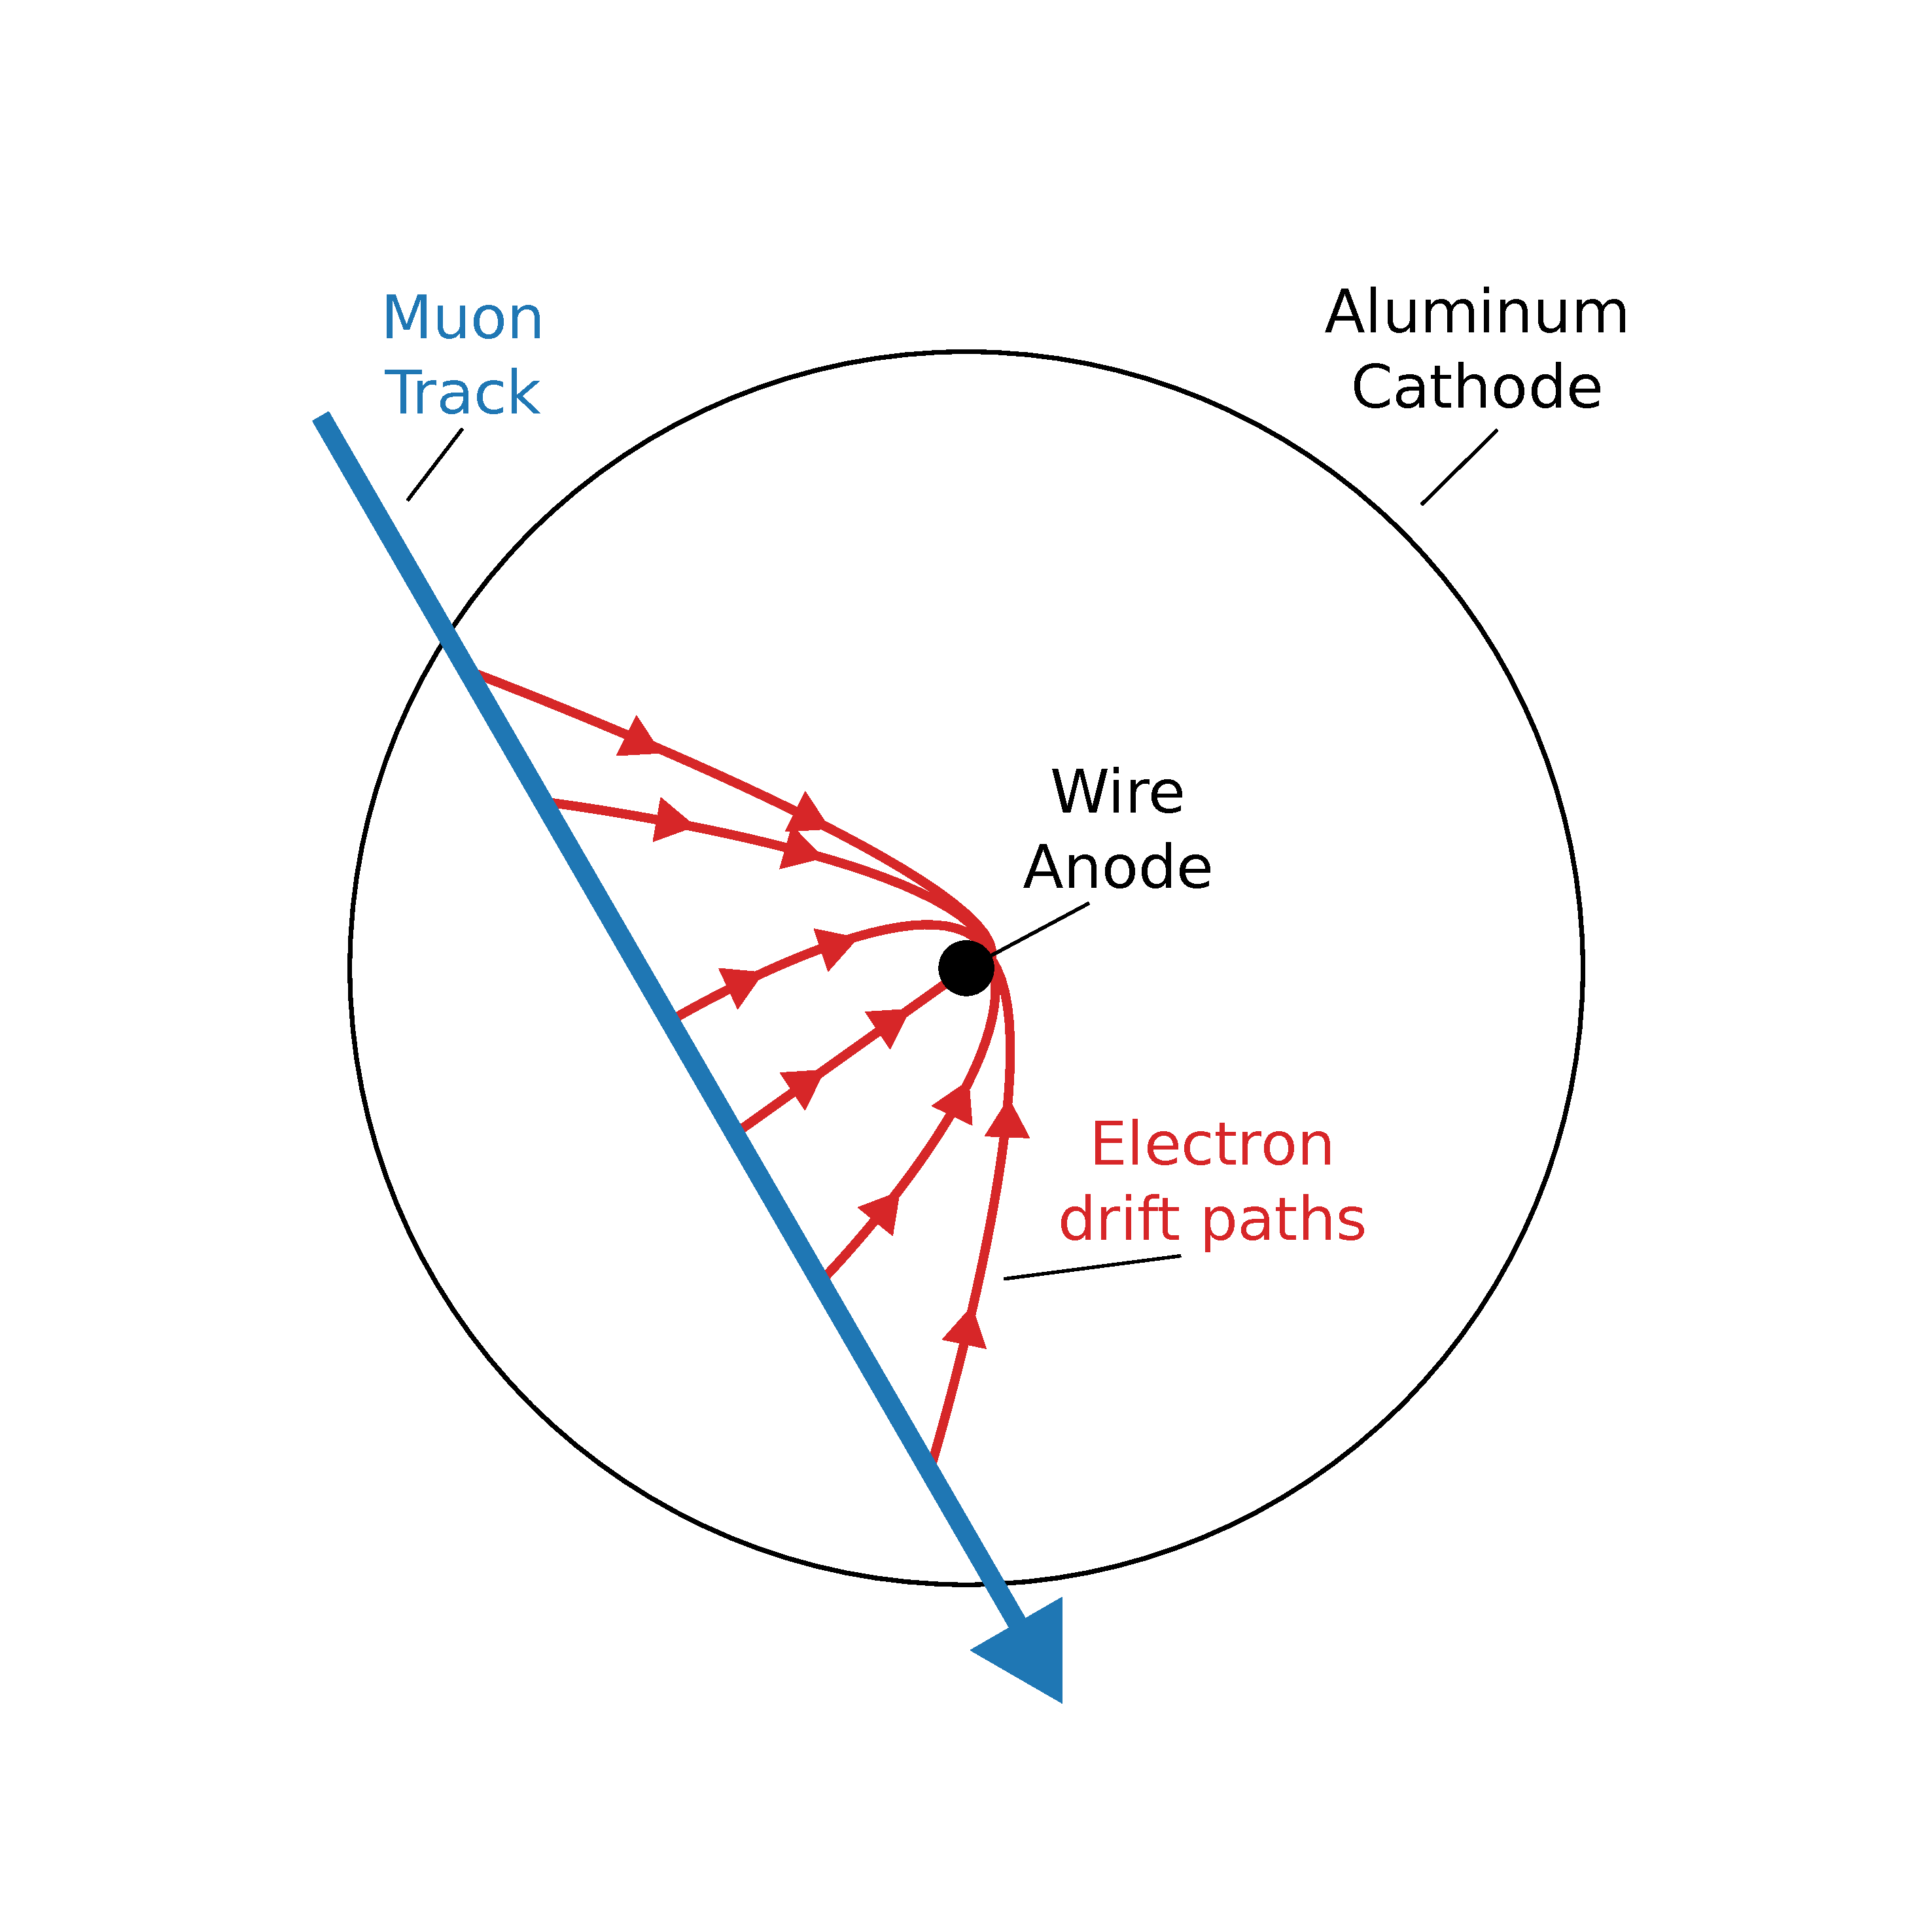
\includegraphics[width=0.5\textwidth]{figures/experiment/mdt/drift.pdf}}}
\subfloat[][]{\label{fig:atlasMdt}{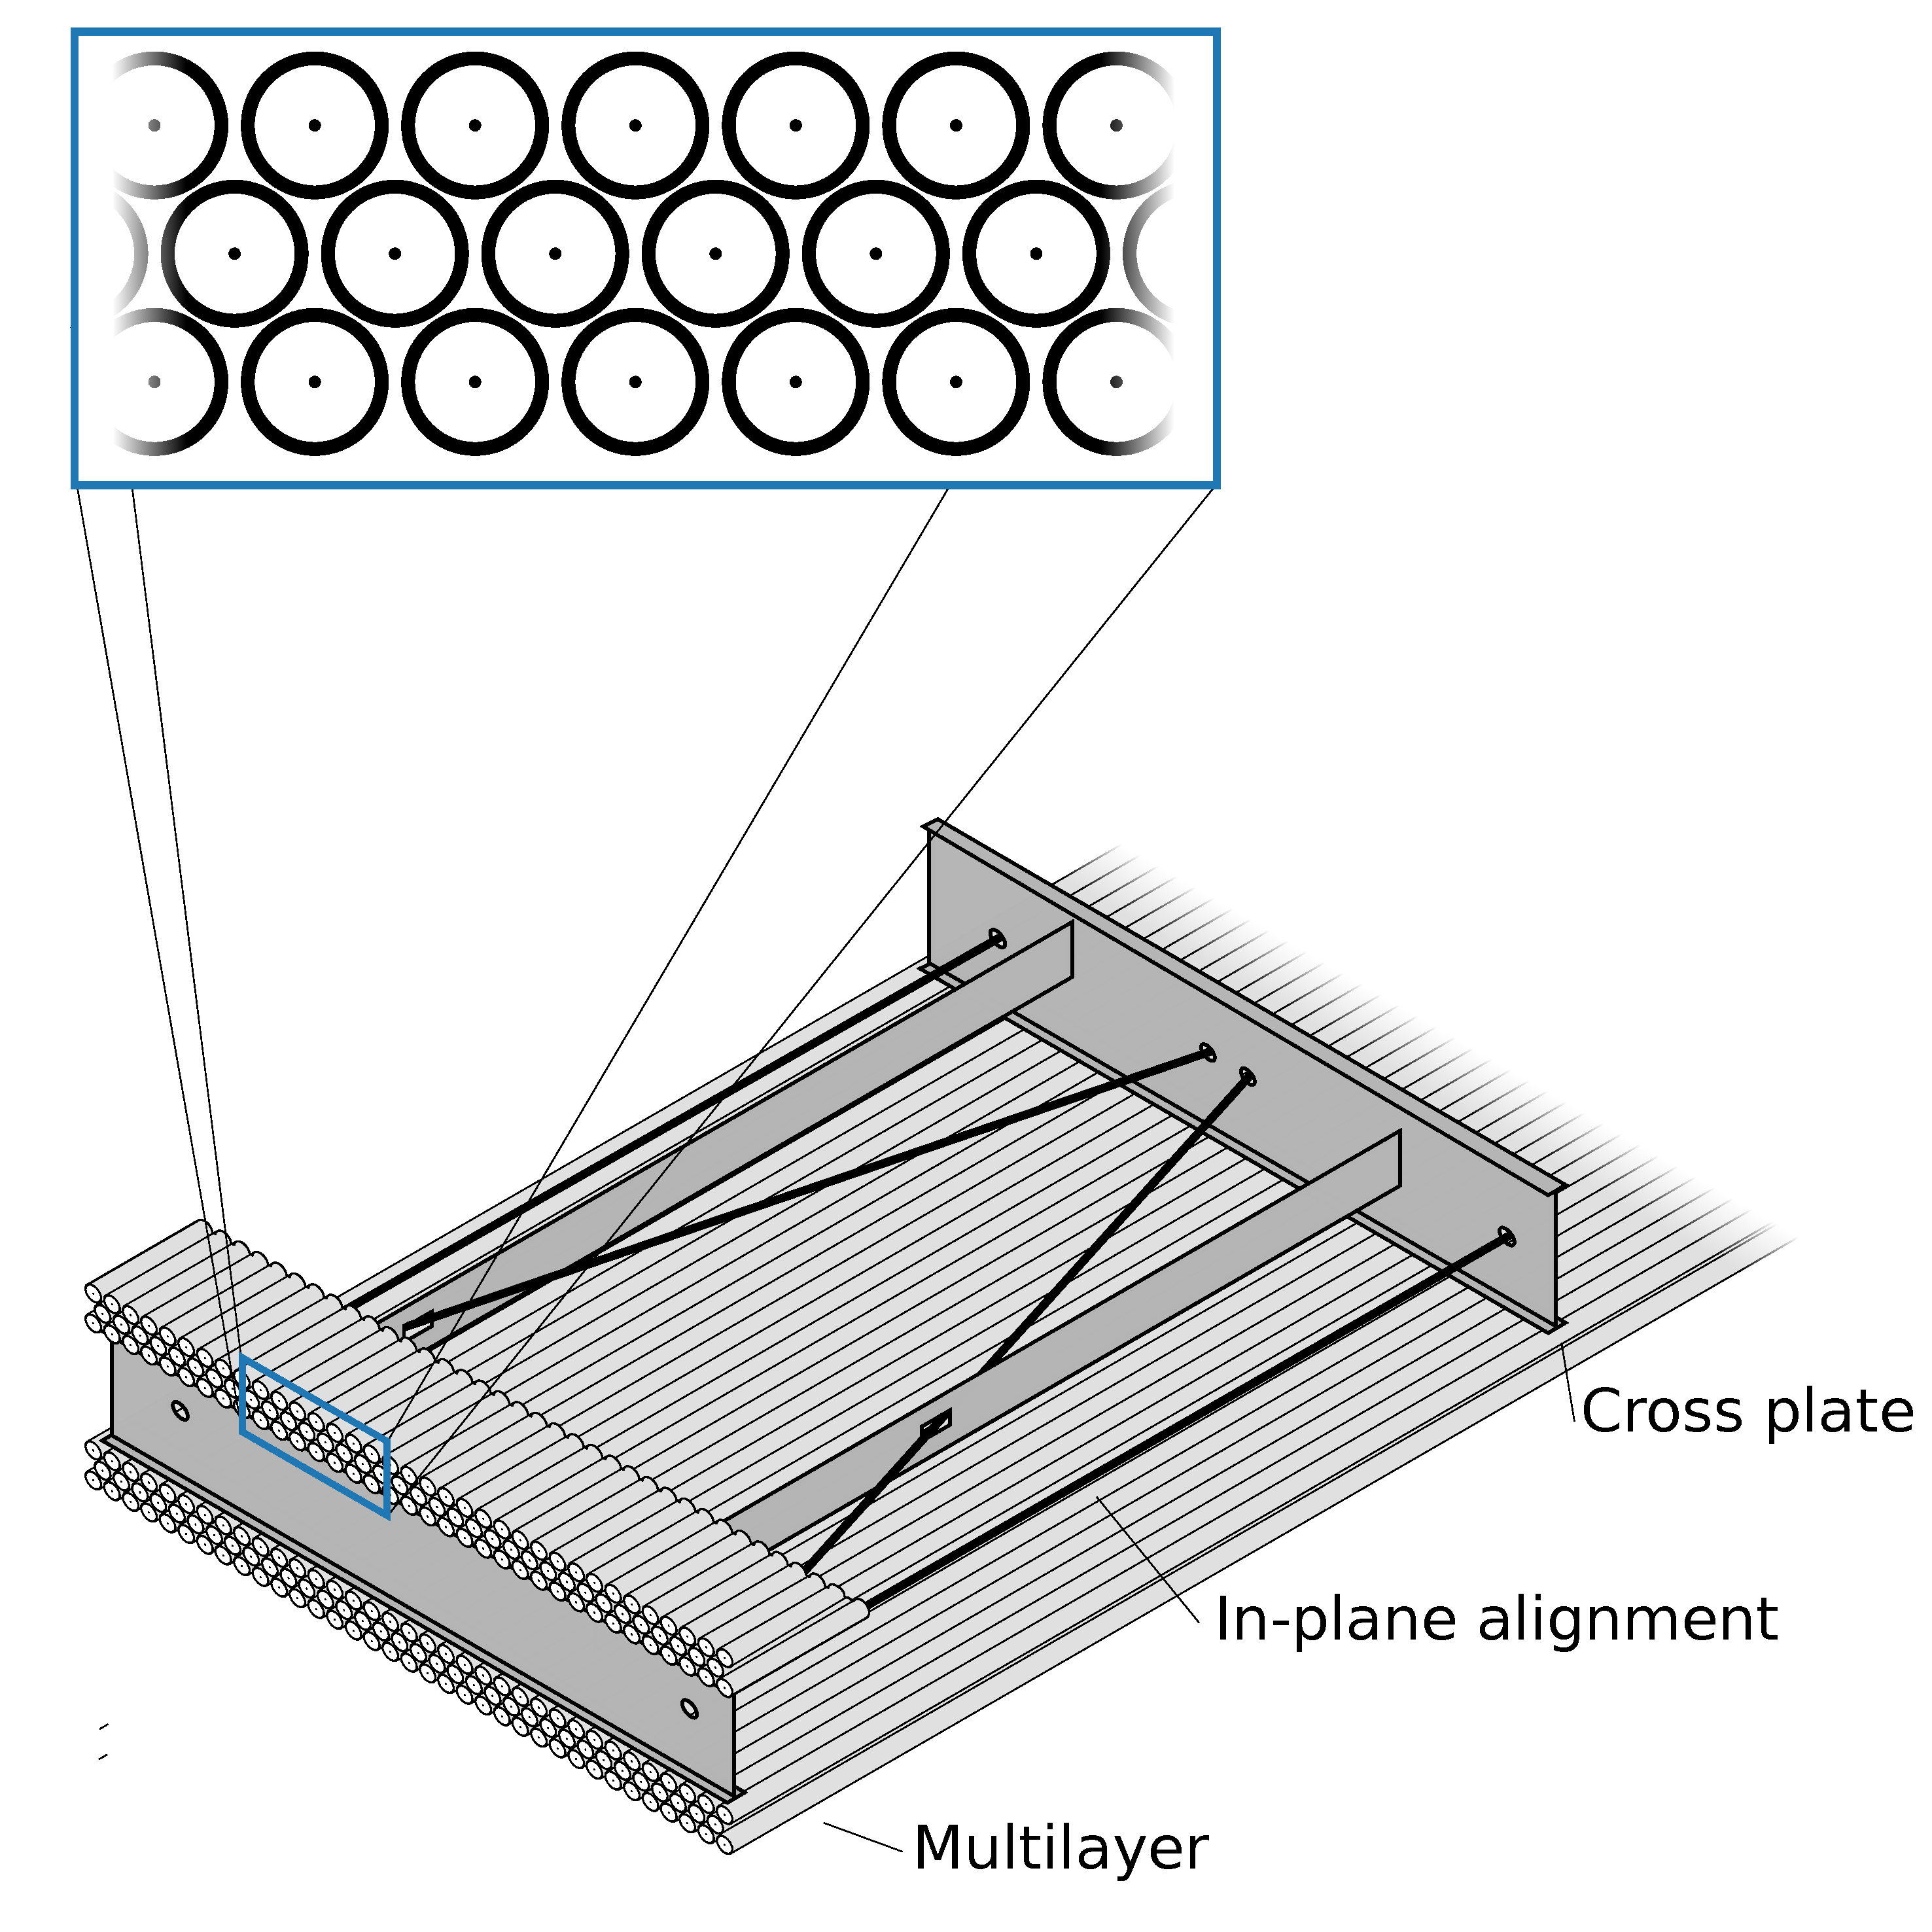
\includegraphics[width=0.5\textwidth]{figures/experiment/mdt/chamber.pdf}}}
% \subfloat[][]{\label{fig:atlasMdt}{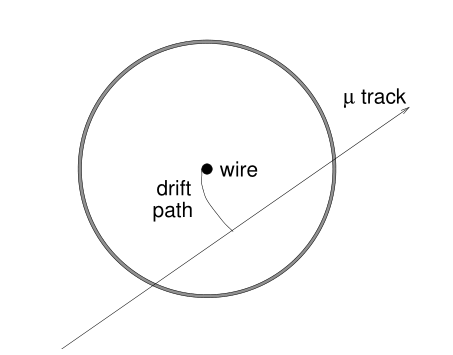
\includegraphics[width=0.5\textwidth]{figures/experiment/atlas/mdt.png}}}
% \subfloat[][]{\label{fig:atlasMdtChamber}{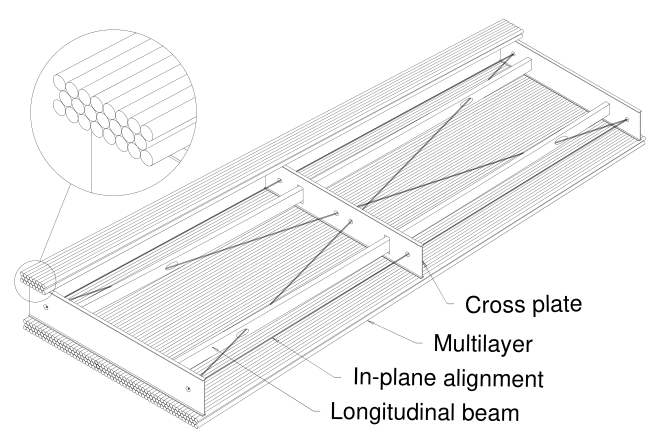
\includegraphics[width=0.5\textwidth]{figures/experiment/atlas/mdtChamber.png}}}
\caption{(a) Cross section of a MDT with a muon track illustrated. Ionizing radiation leaves a track of electrons in the drift gas, which drift towards the positive anode wire and induce a signal. (b) Arrangement of MDTs into multi layers, which are then attached to a support structure to build a chamber.}
\label{fig:atlasMdtChamber}
\end{figure}

The Monitored Drift Tubes (MDT) are the single wire chambers that provide precision muon measurements in the majority of the MS.
An MDT consists of a 30~mm aluminum tube cathode with a central 50\um gold-plated tungsten-rhenium wire anode.
The tube is filled with a mixture of argon (91\%), nitrogen (4\%), and methane (5\%) pressurized to 3~bar.
Charged particles passing through the tube ionize the gas, freeing a track electrons to drift towards the 3.08~kV wire over the course of $\approx750$~ns.
The spatial resolution of a single MDT is 80~\um.
This is shown in Figure \ref{fig:atlasMdt}.
The radial displacement of the track is determined from the total drift time.
Layers of MDTs are laminated together with glue and affixed to a support frame that holds them precisely in positions.
This is shown in Figure \ref{fig:atlasMdtChamber}.
The central cross plate is adjustable to bend the outer aluminum tubes to match the gravitational sag of the anode wires.
The deformation of the chamber is monitored by built-in optical systems.

As shown in Figure \ref{fig:atlasMs}, the MDT chambers are used throughout ATLAS except in the very high pseudorapidity region where particle flux exceeds their measurement rate.
In the barrel ($|\eta|<1$), chambers are rectangular and arranged into three layers beginning outside the calorimeters.
In the end-cap ($|\eta|>1$), chambers are trapezoidal and positioned radially on either an inner or outer wheel.
The MDT system is comprised of 1194 precision chambers, with a total of 370,000 output channels  \cite{muonTdr}.

\subsubsection{CSC} % precision

\begin{figure}[h!]
\captionsetup[subfigure]{position=b}
\centering
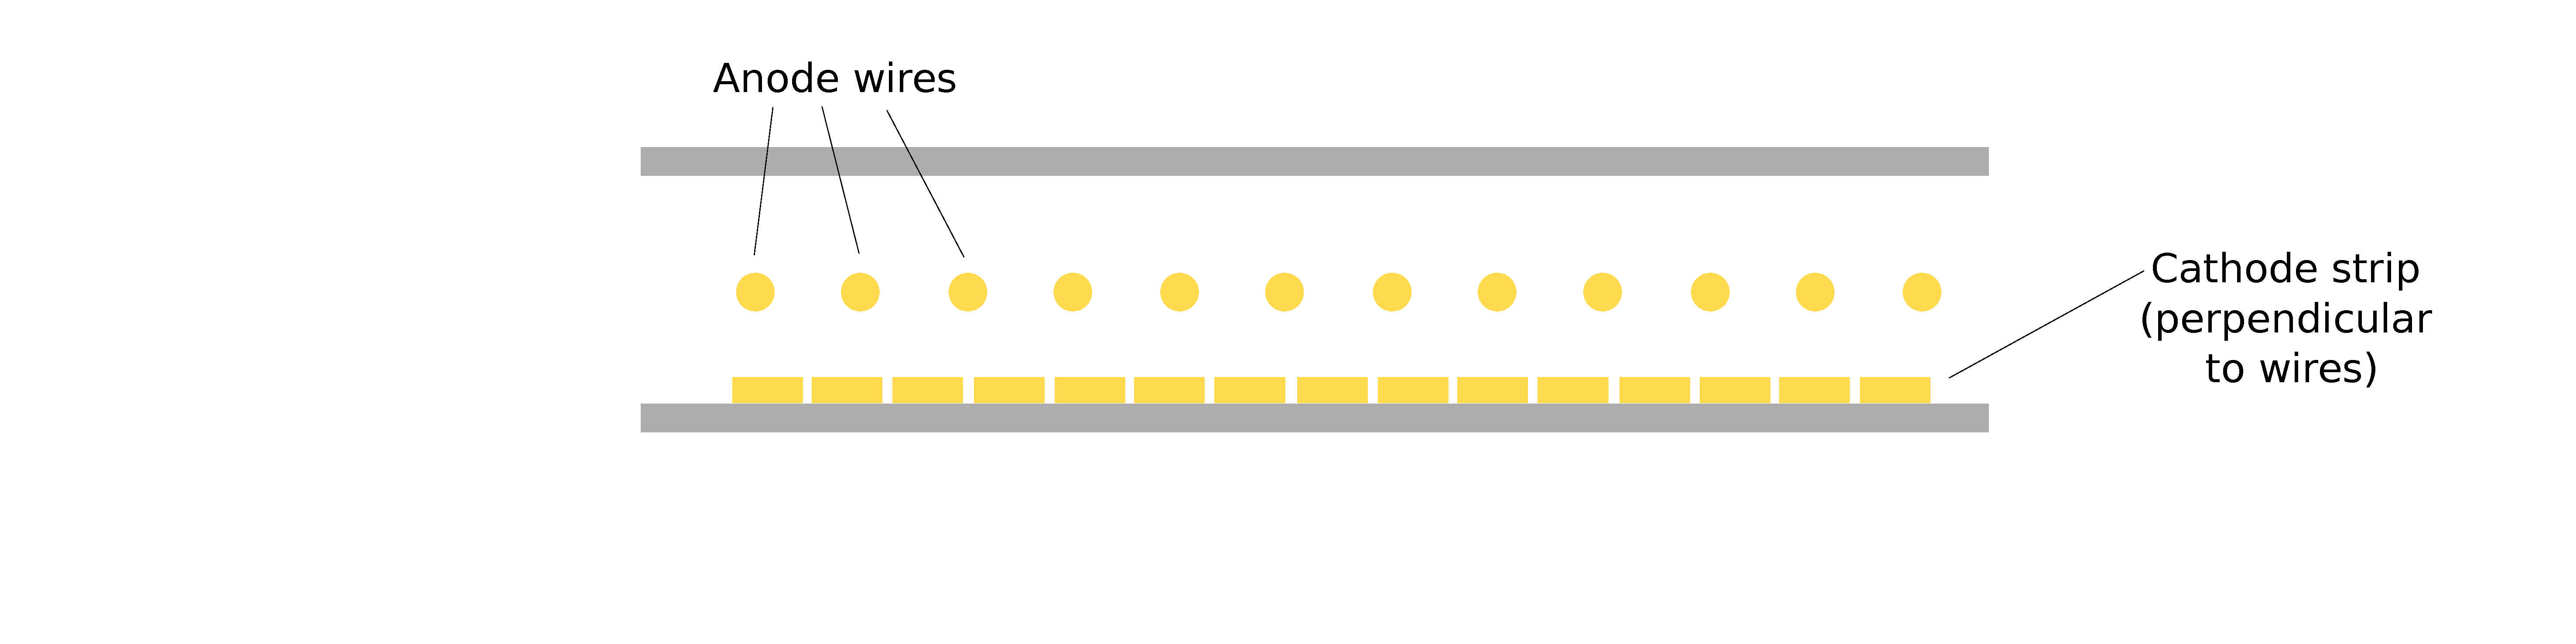
\includegraphics[width=1.0\textwidth]{figures/experiment/mdt/csc.pdf}
\caption{Cross section of a CSC, showing multiple anode wires and cathode strips.}
\label{fig:atlasCsc}
\end{figure}

The Cathode Strip Chambers (CSC) are multiwire proportional chambers that provide precision muon measurements in the region close to the interaction point and the beamline ($2<|\eta|<2.7$).
The CSCs are designed to have short drift times ($<30$~ns) to avoid saturation from the high particle flux in this region.
Like the MDTs, the spacial resolution of CSCs is 80~\um.
They consist of anode wires strung perpendicularly to cathode strips, as shown in Figure \ref{fig:atlasCsc}.
The wires in the CSCs are 30~\um versions of those used in the MDTs, and the cathode strips are copper adhered to glass-reinforced epoxy.
Four of these constructions are stacked on top of each other, separated by a closed-cell foam, to complete a CSC chamber.
The intermediate area is filled with a mixture of carbon dioxide (50\%), argon (30\%), and carbon tetrafluoride (20\%).

When an ionizing particle passes through the CSC, it produces an electron avalanche onto adjacent anode wires.
This induces a charge on the cathode strips, which in turn is amplified and read out.
Long cathode strips provide coarse information, while short segmented cathodes provide precision hit data.
The CSC system is comprised of 32 precision chambers, with a total of 67,000 output channels  \cite{muonTdr}.

\subsubsection{Trigger Chambers}

The MDT and CSC chambers are supported by additional chamber types that provide rapid data for the trigger decision.
These are the Resistive Plate Chambers (RPC) in the barrel, and the Thin Gap Chambers (TGC) in the end-caps.
These are positioned in close proximity to a corresponding precision chamber.
The RPCs consist of two resistive plates coated in thin layers of graphite, held at 8.9~kV.
A 2~mm gap between the plates is filled with gas (tetrafluoroethane with 3\% isobutane).
An ionizing particle passing through the gap instigates an electron avalanche, which is read out by conductive strips on both sides of the gap.
The strips are orthogonal to each other.
Two RPC layers are combined in a station, separated by a 6~mm support.
The RPC system is comprised of 596 trigger chambers, with a total of 355,000 output channels.
The TGCs are multiwire proportional chambers with a small 2.8~mm gap.
The 50~\um anode wires are held at 3.1~kV, and the chamber is filled with carbon dioxide (55\%) and $n$-pentane (45\%).
The TGC system is comprised of 192 trigger chambers, with a total of 440,000 output channels  \cite{muonTdr}.

\subsection{Magnet System}
\begin{figure}[h!]
\captionsetup[subfigure]{position=b}
\centering
\subfloat[][]{{
\includegraphics[width=0.3\textwidth]{figures/experiment/atlas/mags/end.pdf}}}
\subfloat[][]{{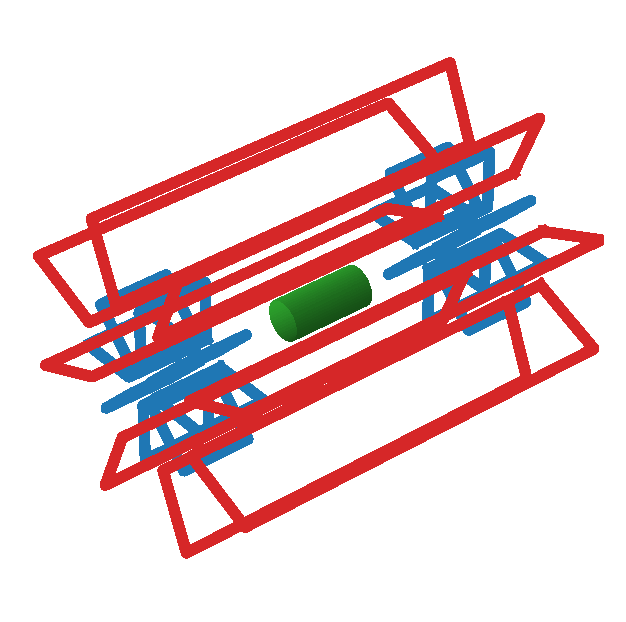
\includegraphics[width=0.3\textwidth]{figures/experiment/atlas/mags/perspective.pdf}}}
\subfloat[][]{{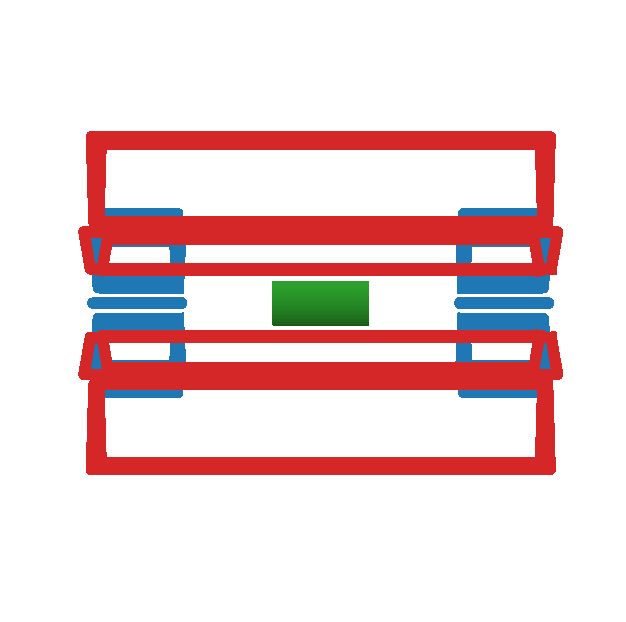
\includegraphics[width=0.3\textwidth]{figures/experiment/atlas/mags/side.pdf}}}
\caption{Illustration of the geometry of the magnet system field coils showing (a) the endcap, (b) perspective, and (c) the side view. The Central Solenoid (green) is inside the eight windings of the Barrel Toroid (red). End-Cap Toroids (blue) appear on either side.
}
\label{fig:atlasMagnets}
\end{figure}

%magnet
The ATLAS Magnet System is composed of three superconducting magnet systems: the Central Solenoid, the Barrel Toroid, and the two End-Cap Toroids.
The arrangement of these magnets is shown in Figure \ref{fig:atlasMagnets}.
The purpose of these magnets is to produce a strong magnetic field to enable the measurement of momenta of charged particles.
Each coil that makes up the magnets is effected not only by gravity but also by magnetic forces.
To support them, each coil is enclosed in a mechanical structure that also houses cooling circuits and cryostats to maintain its operating temperature of $\sim4.5$~K.
The coils are wound with superconducting niobium-titanium in a copper-aluminum matrix.
When the four magnets are fully energized, the magnet fields store an energy of 1.3 GJ. \footnote{This is equivalent to the energy released by an explosion of 300 kg of TNT}

The large Barrel Toroid (BT) magnet is one of the most visible features of the experiment.
The magnet is the largest in ATLAS and spans 26~m along the beamline with a diameter of 20~m.
It consists of eight air-cooled coils surrounding parts of the muon spectrometer.
The coils each contain 120 turns, and the coils are wired in series.
At its strongest, the field of the BT reaches 3.9~T.
Finally, two air-cooled End-Cap Toroids (ECT) provide a magnetic field for the MS wheels.
These have a length of 5~m and an outer diameter of 10.7~m. An inner diameter of 1.65~m is left empty to allow passage of the beam.
Like the BT, both ECTs consist of eight coils, but with 116 turns.
All 16 ETC coils are wired together in series.
The fields of the ETC reach a peak of 4.1~T.
Both toroids are operated with a current of 20 kA.
Tubes carrying 4.5~K helium are welded onto the casings of the windings to keep them at superconducting temperatures.

The innermost magnet is the cylindrical Central Solenoid (CS), which is 5.3~m long and 2.4~m in diameter.
The CS produces a magnetic field of 2.0-2.6~T in the region of the inner detector.
The coil consists of a single layer coil wound 1173 times around a cylinder.
To reduce the amount of material that particles can interact within the inner detector, the CS shares a vacuum vessel and cryostat with the Liquid Argon Calorimeter  \cite{magnetTdr}.

\subsection{Trigger System}

\begin{figure}[h!]
\captionsetup[subfigure]{position=b}
\centering
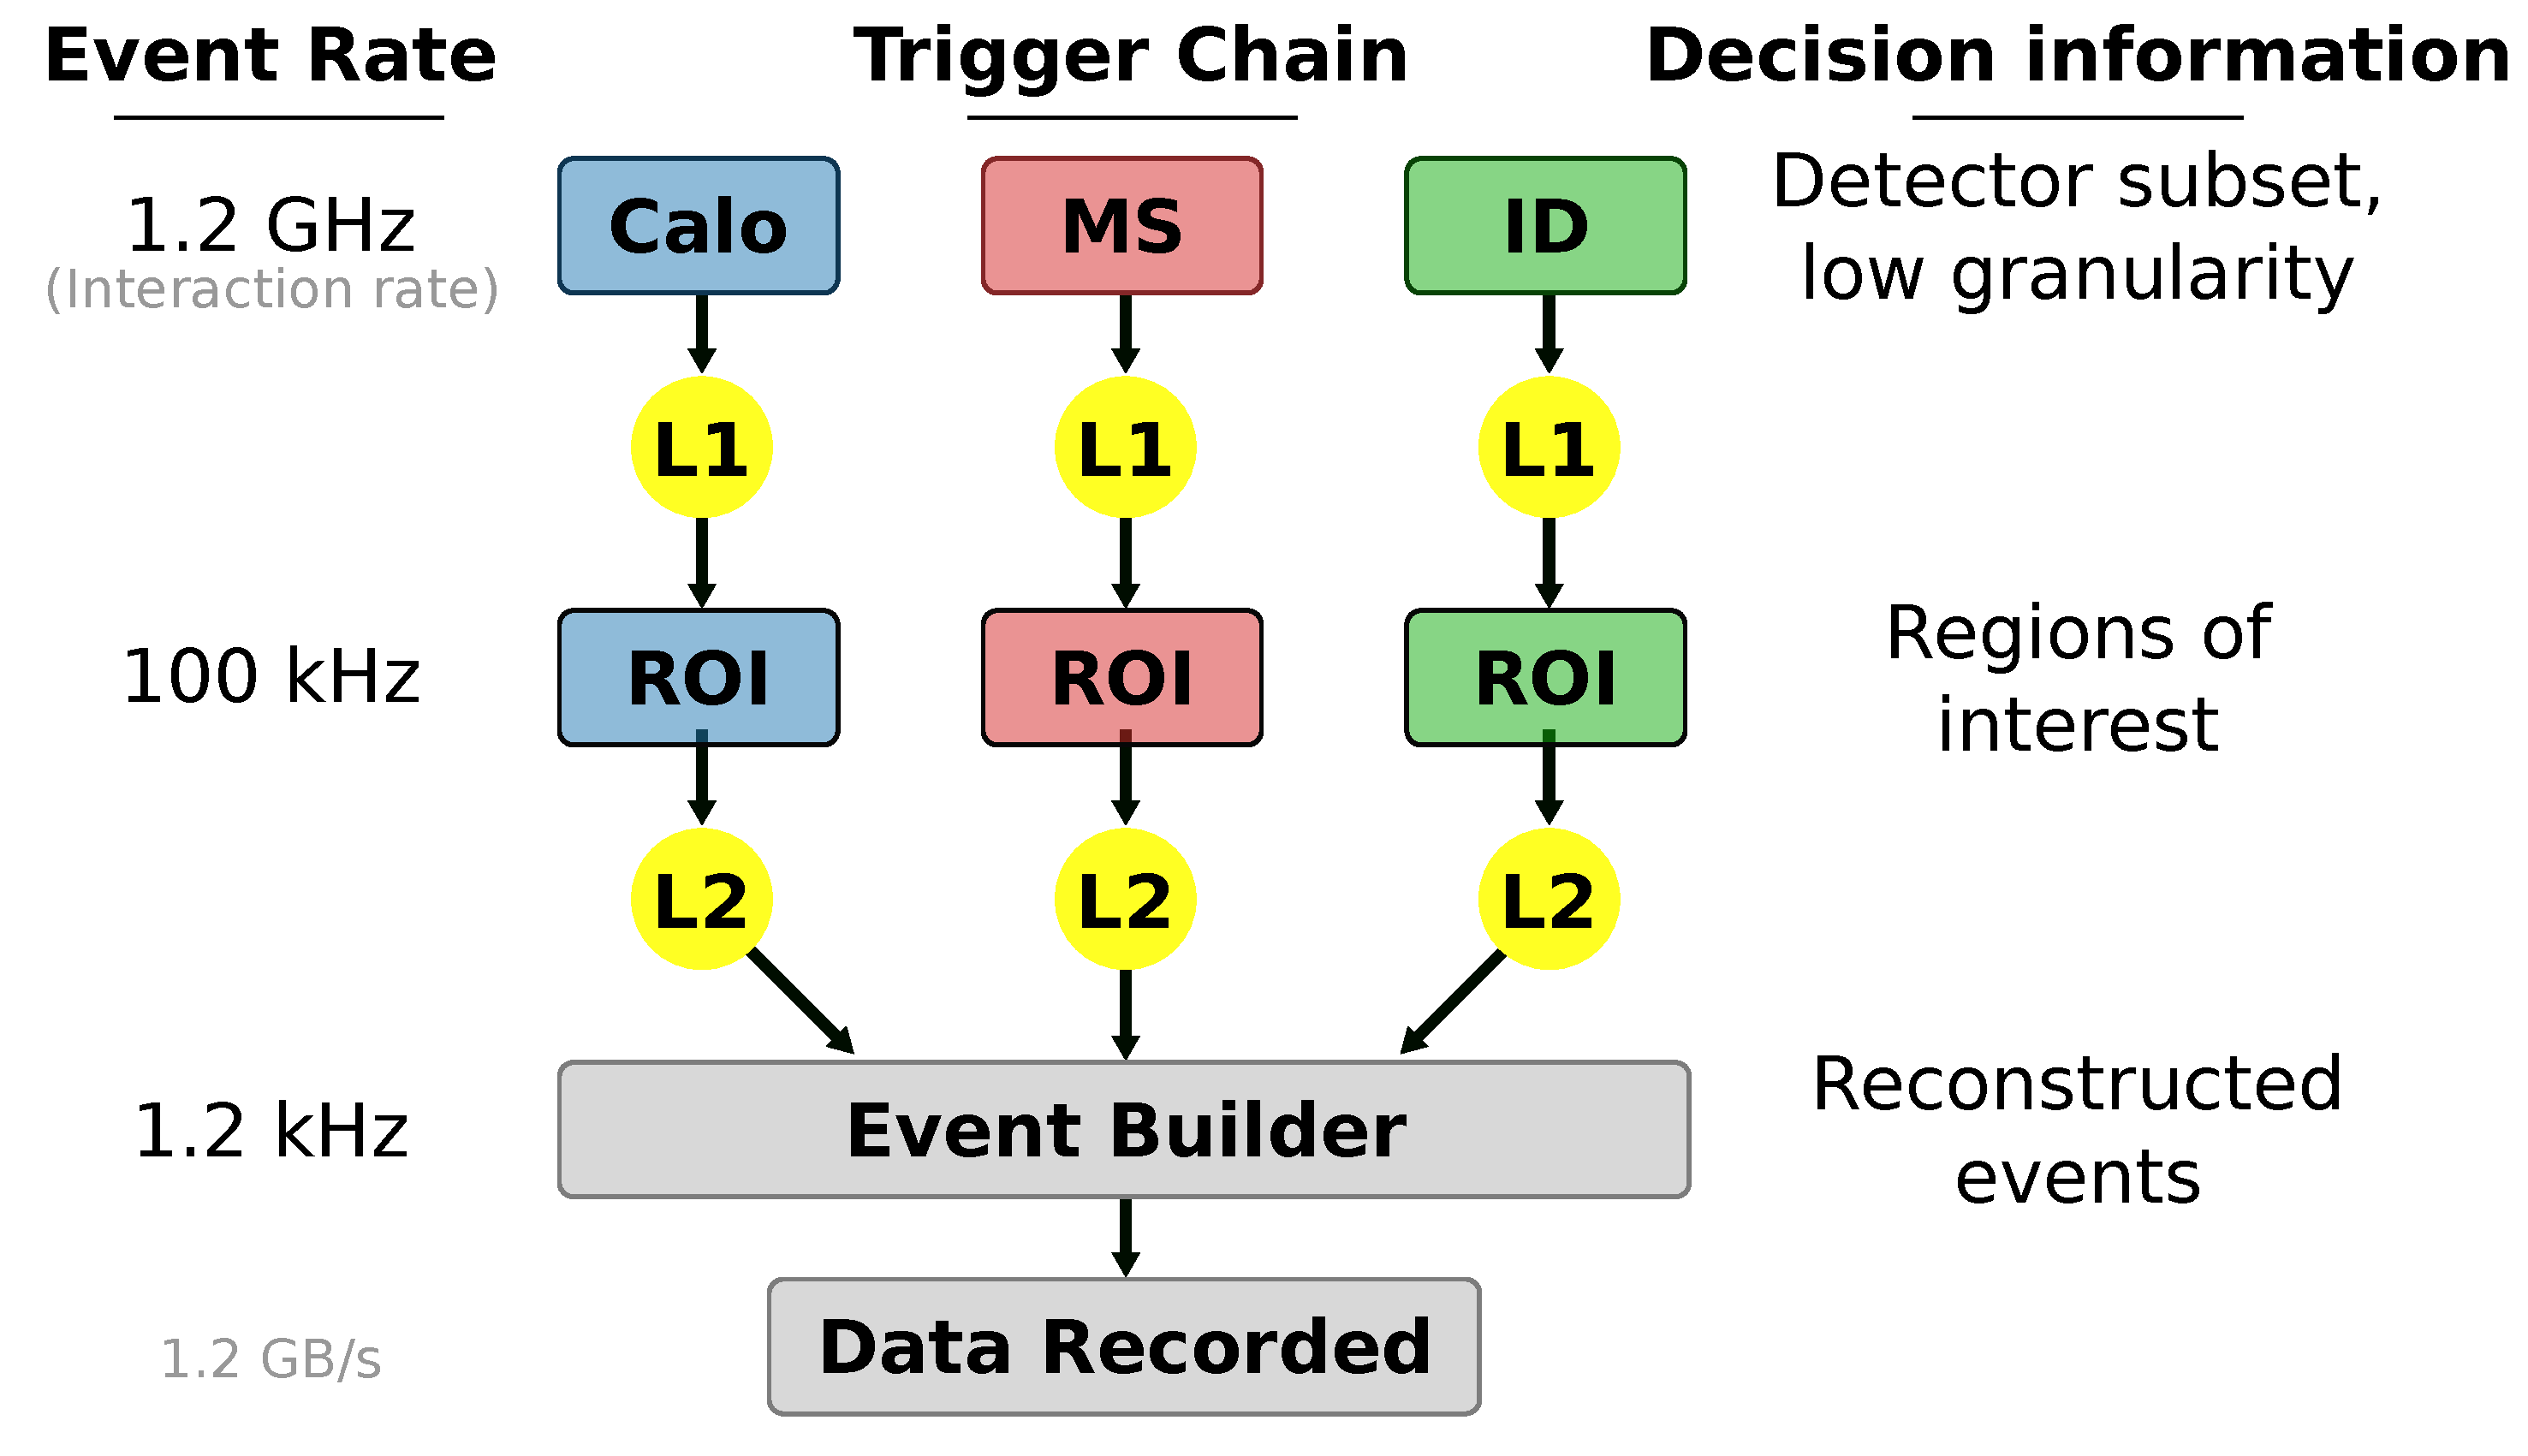
\includegraphics[width=0.8\textwidth]{figures/experiment/atlas/trigger.pdf}
% 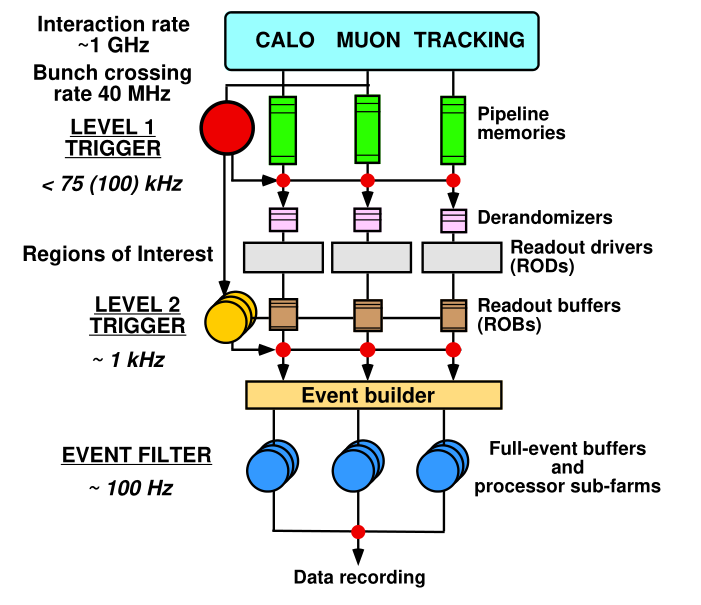
\includegraphics[width=0.7\textwidth]{figures/experiment/atlas/trigger.png}
\caption{Flow of data through the trigger system. Trigger decisions are indicated in yellow.}
\label{fig:atlasTrigger}
\end{figure}

The nominal 24.96~ns bunch spacing for LHC beams results in 40 million bunch crossings per second.
A beam with a luminosity of $1.5\times10^{34}$\cms produces approximately 30 collisions per bunch crossing.
This results in approximately 1.2 billion collisions per second.
Data is read from approximately one hundred million electronic output channels across approximately three million meters of cables during operation.
The data recorded from a typical event is 1.5~MB, resulting in 156~EB worth of data generated by ATLAS per day.
\footnote{For comparison, this volume of collected and processed data is a sizable fraction of humanity's existing storage and roughly 30,000 times the total data collected by the Event Horizon Telescope project.}
The Trigger System is responsible for rapidly sorting through this data and selecting events to record and events to discard.
It takes hit information from the ID, MS, and calorimeters and searches for signatures of interesting collisions.
The trigger decision is made by computers in the nearby underground service area (USA15), so data must first be transmitted to these.
A schematic of the trigger system is shown in Figure \ref{fig:atlasTrigger}.

The first rejection of events reduces the event rate from $\approx1.2$~GHz to $\approx100$~kHz is performed by the Level-1 (L1) Trigger.
This selects searches for the signatures of interesting particles (high-\pt muons, electrons, jets, and others) in a subset of the detectors.
When an event passes the L1 trigger, it sends an ``accept'' signal is sent back to the detector.
Meanwhile, various front-end electronics have stored precision hit data.
When they receive an L1 accept, they transmit this data off the detector to USA15.
Since the front-end electronics must store hit information while waiting for a possible L1 Trigger decision, the target time frame for this is 2~\us \cite{triggerTdr}.

The data is sent from the detector into \emph{readout buffers} (ROB) for temporary storage while the Level-2 (L2) Trigger evaluates the event with a broader set of criteria.
The L2 trigger reduces the event rate down to $\approx1.2$~kHz.
It works by searching \emph{regions-of-interest} (ROI) constructed by the preliminary L1 trigger information.
Based on the $\eta-\phi$ location of the ROI, the trigger logic accessed the precision data stored in the ROBs.
This process takes longer than the L1 decision, on the order of 10~ms.
With the precision data available, the L2 trigger can make strict requirements on the kinematics of various objects.
For example, this analysis uses muon and electron triggers that require leptons passing certain thresholds of \pt or \et, respectively.
Events passing the L2 trigger are passed along for full reconstruction and storage \cite{atlasTriggerNew}.
% The fully reconstructed events from the \emph{Event Builder} are filtered by the Event Filter, which reduces the rate down to  $\approx$100~Hz.
% \cite{triggerTdr}

% 
\section{Physics Object Reconstruction}\label{sec:physObjects}
The analyses presented in this thesis view the data collected by the ATLAS experiment through the abstraction of \emph{physics objects}.
It is worth noting that physics objects are not exactly isomorphic to the actual physical entities emanating from the collision.
These are patterns of detector hits and energy deposits that are construed to have some physical meaning.
In some cases, these patterns are clearly identified with particles like muons or electrons passing through the detector.
In other cases, the identification is more pragmatic for the purpose of analysis, as is the case when describing \emph{missing transverse momentum} ($E_T^\text{miss}$) as an object.
Somewhere in between these are clusters of energy deposits called \emph{jets}, which are identified as the result of the hadronization of quarks and gluons.

The difference between the ``physics object'' of a jet and the quark or gluon it is presumed to describe is clear.
Different definitions of ``cluster'' lead to different jet energies, and even different numbers of jets.
This subtlety in definition also applies to muons, electrons, and of course, $E_T^\text{miss}$.
The following section describes the choices made in defining the physics objects used in this thesis.

There are three steps in choosing what physics objects to use.
The first step is in the reconstruction algorithm, which arranges the data recorded in an event into reasonable approximations of particles and jets.
Next, some of these candidates are accepted or rejected based on identification criteria.
Finally, a secondary requirement of isolation is imposed on the objects to isolate objects originating directly, or promptly, from the collision.
This final step is particularly important in the context of this thesis, where prompt leptons are of primary interest.

\subsection{Electrons}
Electrons are reconstructed from data collected by the inner detector and electromagnetic calorimeter.
An electron passing through the ID typically produces four hits in the pixel layers and eight hits in the Silicon Tracker (SCT) layers, from which the track and impact parameter are established.
After passing through the silicon detectors, the electron produces transition radiation surrounding the Transition Radiation Tracker (TRT).
This helps identify electrons as relativistic charged particles.
Next, the electron enters the electromagnetic calorimeter, where it deposits most of its energy.
The segmented structure of the calorimeter measures both the energy deposited directly by the electron and subsequent showers of secondary particles.

The search for electron candidates begins with a scan of energy deposits in the calorimeter, searching for localized clusters in $\eta-\phi$ space.
Next, the hits in the inner detector pixel and SCT layers are grouped first by layer and then between layers to form tracks.
Calorimeter clusters with azimuth $\phi_\text{calo}$ and ID tracks with azimuth $\phi_\text{track}$ are matched with a fitting procedure.
A restriction $-0.10<\Delta\phi<0.05$ where $\Delta\phi=-q\times(\phi_\text{calo}-\phi_\text{track})$ and $q$ is the charge of the track is made, and the asymmetric range accounts for bremsstrahlung effects \cite{elecReco}.

\subsubsection{Identification}

The choice of which electron candidates to consider for analysis is made using a likelihood (LH) identification.
This quantifies the probability for a candidate electron to have been produced by a physical electron passing through the detector.
The goal is to identify prompt electrons (signal) from jets, photon conversion electrons, and hadronic decay electrons (background).
Fourteen quantities, $\vec{x}$, are measured for the candidate electron.
These quantities describe the distribution of energy in the calorimeter layers, the impact parameter from the ID, the momentum lost by the track over time, the TRT response, and the $\eta-\phi$ match between the track and calorimeter cluster.
The PDFs for their values, $\vec{P}_{S(B)}$, are measured from simulation for signal and background.


The likelihood for a candidate to be signal (background) is given in Equation \ref{eqn:elecLH}.
\begin{equation}\begin{split}\label{eqn:elecLH}
L_{S(B)}(\vec{x}) = \prod_{i=1}^{14}P_{S(B),i}(x_i)
\end{split}\end{equation}
The discriminant $d_L$ is defined in Equation \ref{eqn:discLH} and peaks near one for signal, and zero for background.
\begin{equation}\begin{split}\label{eqn:discLH}
d_L=\frac{L_S}{L_S+L_B}
\end{split}\end{equation} 
Electron candidates passing increasingly restrictive thresholds of $d_L$ comprise the \code{VeryLoose}, \code{Loose(AndBLayer)}, \code{Medium}, and \code{Tight} LH identification working points.
In this thesis, the \code{LooseAndBLayer} and \code{Medium} LH identifications are used.
Both additionally require at least two pixel hits and seven total hits in the silicon ID.
At least one pixel hit is required in the innermost working pixel layer.
These have efficiencies of 88\% and 80\% for electrons with \et=40~GeV, respectively.

Electrons that are reconstructed with a path traveling directly through a broken calorimeter cell are marked with the label \emph{BADCLUSELECTRON}.
It is helpful to exclude such electrons from consideration due to their poor \et measurement.

% NR:  LooseAndBLayerLLH (QCD Fakes), MediumLLH
% hmm: Medium LH
\subsubsection{Isolation}
The signal models of interest for this thesis lead to electrons produced in isolation from other particles.
These electrons originate promptly from the interaction point.
In order to identify such electrons, the activity within a $\eta-\phi$ cone of $\Delta R=\sqrt{(\Delta\eta)^2+(\Delta\phi)^2}$ is quantitatively by measures of charged tracks and calorimeter energy deposits.
A variable cone size of $\Delta R=\text{min}(0.2,10\text{GeV}/\pt)$ is used to count tracks with $\pt>1$~GeV around the electron. The \pt of the tracks within this cone, excluding the electron's tracks, are summed to define \ptvarconeElec.
The electron's ``tracks'' is plural to account for bremsstrahlung radiation converting to secondary electrons. 
These are counted as part of the electron candidate if the extrapolated track falls within $\Delta\eta+\Delta\phi=0.05\times0.1$ of the primary calorimeter cluster.
Meanwhile, a fixed cone size of $\Delta R=0.2$ is used to sum up the activity in the calorimeters.
First, the energy from the electron is subtracted within an area of $\Delta\eta+\Delta\phi=0.125\times0.175$.
Energy from pileup effects is subtracted, and the remaining \et is summed to define \etcone.

Two isolation schemes are used in this thesis.
The first, \code{FixedCutLoose}, enforces a requirement that $\etcone/\et<0.20$ and $\ptvarconeElec/\pt<0.15$.
The efficiency, $\epsilon_\text{iso}$, of this requirement for prompt electrons is $\approx99\%$.
These cuts perform well in the relatively narrow kinematic region of interest for \hmm, but the search for high-mass phenomena needs a more flexible scheme.
A dynamic isolation, \code{Gradient}, is defined as a function of the electron \et.
It is defined such that the efficiency $\epsilon_\text{iso}=0.1143\times\et+92.14\%$ is constant across $\eta$.
\cite{elecReco}


% NR:  gradient
% hmm: FCLoose

\subsection{Muons}

Data from both the inner detector and muon spectrometer can be used to reconstruct muons.
In the former case, a similar procedure to that used to reconstruct ID electrons is used.
In the latter case, an algorithm searches data from MS chambers for hits that follow plausible muon paths, called segments.
Then, starting from segments, candidate tracks are built by combinatorially including hits from tracks in other layers.
The best tracks are selected based on the $\chi^2$ fit quality and number of hits used.
Each track must contain at least two segments.
\footnote{There is an exception in the transition region between the barrel and endcap where one segment is sufficient, however such muons are excluded from consideration in this thesis.}

\subsubsection{Identification}

Four types of muons are reconstructed.
Combined muons (CB), which are reconstructed using tracks in the ID and MS.
\begin{itemize}
\item Segment-tagged muons (ST), which are built from ID tracks extrapolated to match MS hits.
\item Calorimeter-tagged muons, which are built using ID tracks extrapolated to match calorimeter energy deposits.
\item Extrapolated muons (ME), which are reconstructed using only the MS and the location of the interaction point.
\end{itemize}

Five criteria define the commonly used identifications: \code{Loose}, \code{Medium}, \code{Tight}, \code{Low}-\pt, \code{High}-\pt.
These working points admit or reject muons based on several variables:
\begin{itemize}
    \item The absolute difference between the charge to momentum ratio measured in the MS versus the ID, as a fraction of the sum in quadrature of the corresponding MS and ID uncertainties. This is the q/p significance.
    \item The absolute difference between the \pt measured in the MS vs the ID, as a fraction of the combined \pt. This is the $p'$ variable.
    \item The normalized $\chi^2$ of the combined track fit.
\end{itemize}
% Medium muons
The baseline identification for ATLAS searches is Medium, which begins with CB and ME muons.
CB muons are required to use at least three hits in two MDT layers, or one MDT layer and no more than one missing layer within $|\eta|<0.1$.
The later allowance is made due to lost coverage in the barrel.
ME muons are required to use at least three MDT/CSC layers and fall within $2.5<|\eta|<2.7$, where the ID loses coverage.
For all muons, the q/p significance must be less than seven.
\cite{muonReco}

% Loose muons
The choice of identification depends on the requirements of the analysis.
The searches in this thesis are performed using both expanded and restricted muon identifications.
The \hmm search is concerned with small yields of low-\pt muons; therefore, the \code{Loose} working point is used to maximize reconstruction efficiency.
The \code{Loose} identification is a superset of the \code{Medium} identification.
Additional CT and ST muons are allowed in $|\eta|<0.1$. This adds approximately 2.5\% more muons in the barrel region.
\cite{muonReco}

% High-pt muons
In contrast, the high-mass non-resonant search is concerned with more energetic muons.
For these, a subset of the Medium identification, the \code{High}-\pt identification, is used to reduce incorrectly reconstructed muons.
CB muons otherwise passing the Medium criteria must have three hits in three MS stations.
Some regions of the MS are excluded based on their alignment accuracy.
This restriction trades efficiency to improve \pt resolution by approximately 30\% for muons with $\pt>1.5$ TeV.
It reduces the reconstruction efficiency by $\approx$20\% but improves \pt resolution above 1.5 TeV by $\approx$30\%.
\cite{muonReco}

\subsubsection{Isolation}

As is the case for electrons, the muons of interest in this thesis originate promptly from the interaction point, either from the decay of a Higgs boson or through a contact interaction.
Both types of processes are expected to produce muons that are isolated from other particles in the event.
In contract, semi-leptonic decays and hadronic decays produce muons in close proximity to other particles.
To identify the muons of interest, the concept of isolation is quantified by the sum of tracks in a variable size cone around the muon.
Four related variables are defined.
First variable is \ptvarconeMuon, which is defined as the scalar sum of \pt for tracks within a cone size $\Delta R=\text{min}(0.3,10\text{GeV}/\pt)$. Only tracks with $\pt>1$~GeV are counted, and the muon \pt is excluded.
The second and third variables are \etcone and \ptcone, which are defined as the scalar sum of \et or \pt, respectively, within a cone size of $\Delta R=0.2$.
The fourth variable, \neutralcone, is similar to \etcone. It is the sum of neutral \et within a cone size of $\Delta R=0.2$.

These variables are used to define the three isolation working points used in this thesis.
The first, FixedCutTightTrackOnly, simply required $\ptvarconeMuon/\pt<0.06$.
The second is FixedCutPflowLoose, which requires both $\ptvarconeMuon+0.4\neutralcone)/\pt<0.16$ and $\ptcone+0.4\neutralcone)/\pt<0.16$.
The third is FixedCutLoose, which requires both $\ptvarconeMuon/\pt<0.15$ and $\etcone/\pt<0.30$.
While the efficiency of these isolation requirements varies with \pt, in general, fewer than 1\% of prompt muons are lost.
\cite{muonReco}

\subsubsection{Bad Muon Veto}\label{sec:bmv}

In the high-\pt regime, it becomes difficult to accurately reconstruct muons due to the small bending radius in the magnetic field.
A criteria named \emph{Bad Muon Veto} (BMV) is used to address this by ignoring poorly reconstructed muons in the tails of the relative \pt resolution distributions, $\sigma_{\pt}/\pt$, given in Equation \ref{eqn:muonRes}.

\begin{equation}\begin{split}\label{eqn:muonRes}
    \frac{\sigma(p)}{p}=(\frac{p_0}{\pt}\oplus p_1 \oplus p_2\times \pt)
\end{split}\end{equation} 
The parameters $p_0$, $p_1$, and $p_2$ are measured for the MS and ID in different $\eta$ regions. 
The first term describes uncertainty in energy loss as a muon travels through detector material and becomes less impactful at higher \pt.
The second term covers multiple scattering and irregularities in the magnetic field.
The third term dominates at high-\pt and describes the intrinsic spacial resolution of the muon detectors, including the accuracy of their alignment \cite{muonReco}.
A cut is made on the relative uncertainty:
\begin{equation}
\frac{\sigma(q/p)}{(q/p)} < C(\pt)\cdot \sigma_{rel}^{exp}.
\end{equation}
Here $C(\pt)$ is a \pt-dependent coefficient which is equal to 2.5 when $\pt<1$~TeV and decreases linearly above this.
The application of the BMV reduces efficiency by 7\% for high-\pt muons, while removing poorly reconstructed muons that should not be considered for analysis.

% Isolation
% NR: FCTightTrackOnly
% hmm: FixedCutPflowLoose

\subsection{Jets}\label{sec:expJets}

Strongly charged quarks and gluons exiting a collision hadronize, producing to a collimated jet of heavier particles.
Since none of the final states under consideration in this thesis include quarks or gluons, it is helpful to exclude their presence in some cases.
To this end, jets are reconstructed such that events that contain them may be excluded.
Charged tracks from the ID are associated to calorimeter regions to remove associated deposits using the PFlow algorithm \cite{jetReco}.
The remaining energy is grouped using together by considering pseudo-distance measure between two energy deposits $i$ and $j$,
\begin{equation}\begin{split}
d_{ij} =& \text{min}(p^{-2}_{\text{T}i},p^{-2}_{\text{T}j})\frac{\Delta_{ij}^2}{R^2},
\end{split}\end{equation} 
where $k_{\text{T}i}$ and $p_{\text{T}j}$ are the cluster energies, $\Delta_{ij}=\sqrt{(\Delta y)^2+(\Delta\phi)^2}$ is their separation in rapidity and azimuth, and $R$ is a parameter set to 0.4.
The proceeds by finding the minimum of the set $\{d_{ij},p^{-2}_{\text{T}i}\}$ for all clusters $i$ and $j$. 
If $d_{ij}$ is the minimum, clusters $i$ and $j$ are combined into one.
If $p^{-2}_{\text{T}i}$ is the minimum, then cluster $i$ is considered to be a jet and is removed from the set.
Minima are found and removed until none remain.
This defines all the jets in the event \cite{antikt}.

Jets originating from bottom quarks and the decay of B-hadrons (b-jets) are of particular interest for the \hmm analysis.
A multivariate discriminant, MV2c10, is helps to distinguish b-jets from other light jets \cite{btag}.
This separates the b-jets from light flavor jets based on the characteristic displaced vertices of their associated tracks.
An identification that tags 85\% of b-jets defines the ``b-tag working point'' that proves useful to reject events, including b-jets.

\subsection{Missing transverse momentum}

The final ``object'' to consider in events is the missing transverse momentum, \met.
The transverse momenta of muons, electrons, and the remaining tracks in the ID are summed to produce the total measured \pt of the event.
Since the total \pt of the initial state is close to zero, the negative of this \pt sum represents the \pt of objects that have not been reconstructed \cite{met}.
The \met of an event is a helpful proxy for high-\pt neutrino, which carry \pt without detection.
This makes \met useful in the \hmm search when identifying the decay of \W to leptons and neutrinos.
In events with high-\pt muons, mis-measured muon \pt also appears in the \met sum.
This makes \met useful in the search for high-mass phenomena to study such muons.


\chapter{Phenomenology of Proton Collisions}\label{sec:phenomenology}

\section{Physics at Hadron Colliders}

The LHC collides protons with the highest center-of-mass-energy, \sqrts, ever achieved by particle colliders.
During a collision, the constituents of the proton may interact directly and exchange a substantial fraction of their proton's momentum, in a process called hard-scattering.
The hard-scattering interaction may be quark-quark, quark-gluon, or gluon-gluon scattering events.
These scattering amplitudes may be predicted theoretically and compared to experimental measurements.
% that can be described with a degree of fidelity by a matrix element complication.
This is a messy process and is complicated by the composite nature of the protons.
This section describes how colliding protons may produce events that are of interest to the physics analyses in this thesis.

\subsection{Parton distribution function}

\begin{figure}[h!]
\captionsetup[subfigure]{position=b}
\centering
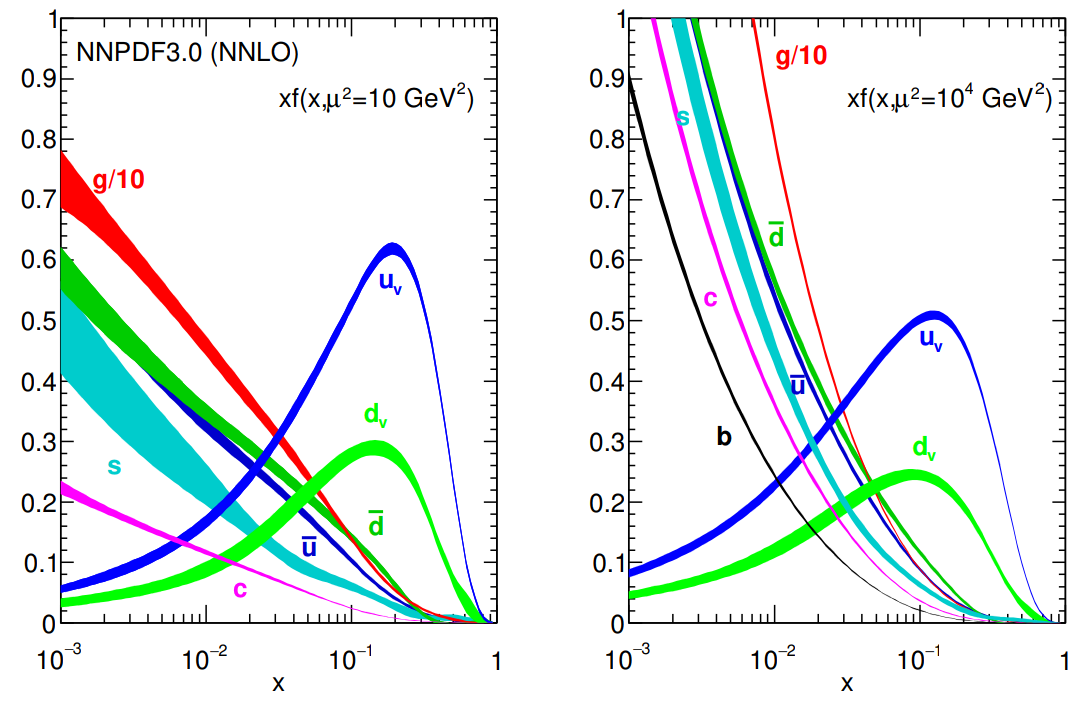
\includegraphics[width=0.99\textwidth]{figures/pheno/pdgpdf.png}
\caption{Parton distribution functions $xf_i(\feynx,Q)$ calculated using NNPDF3.0 with energy scale $Q^2=10\text{~GeV}^2$ (left) and $Q^2=10^4\text{~GeV}^2$ (right). This figure is from \cite{Ball:2014uwa}.}
\label{fig:partDistFunc}
\end{figure}

The protons that make up the colliding beams at the LHC are bound states of quarks and gluons, collectively called partons.
These consist of three valance quarks ($uud$), and a \emph{sea} of virtual quark/anti-quark pairs.
When two protons collide with sufficient energy \footnote{On the scale of $\Lambda_\text{QCD}\approx218$~MeV.}, two types of qualitative processes take place.
First is \emph{hard-scattering}, an interaction mediated by a large momentum exchange between typically two partons.
Second is \emph{soft-scattering}, where the remaining partons interact through the low energy mediators.
While both processes are interesting, hard-scattering interactions are of particular interest in this thesis, as these provide access to particularly high energy interactions.

When two partons interact each carries a fraction of their respective proton's total energy, $\sqrts/2$.
% based on Bing comment, define longitudinal earlier
The longitudinal component of the momentum fraction, $\feynx$.
When a high energy probe particle collides with a proton, the probe will hard-scatter off of one of the proton's constituents, be it a quark or gluon.
In $pp$ collisions, the probe is a parton selected randomly from a proton in the opposing beam.
The probability of the probe to scatter off a particular parton $i$ depends both on its momentum fraction $\feynx$ and on the momentum exchange $Q^2$.
This differential probability function, $f_i(\feynx,Q^2)$, is called the parton distribution function (PDF).
Hence, $f_u(\feynx,Q^2)$ gives probability the that the probe will interact with an up quark, while $f_{\overline{s}}(\feynx,Q^2)$ gives the corresponding probability for an interaction with an anti-strange quark.

The proton dynamics that determine PDFs occur at low $Q^2$, where calculations are complicated by the large QCD coupling from Equation \ref{eqn:alphas}.
Instead of analytic calculations, PDFs functions are fit to experimental measurements.
The resulting PDF shapes as a function of $\feynx$ is shown in Figure \ref{fig:partDistFunc} for each parton.
The valence quarks ($u$ and $d$) are seen to have probability peaks between $\feynx=0.1$ and $\feynx=0.2$, indicating a relatively high frequency that these carry a large portion of the proton's momentum.
In contrast, the sea quarks ($\overline{u}$, $\overline{d}$, $s/\overline{s}$, and $c/\overline{c}$) typically carry a much smaller momentum fraction.
The $u$ and $d$ quarks contribute to the sea as well, and Figure \ref{fig:partDistFunc} separates the valance component from the sea component for these.
The PDFs of the sea $u$ and $d$ quarks and anti-quarks are identical since these are produced in virtual pairs.
The PDFs for gluons are shown scaled down by a factor of 10, as nearly half the proton's momentum is carried by gluons \cite{wells}.

The differential cross sections of an $2\to X$ interaction (given in appendix Equation \ref{eqn:diffCrossSection}) depend on the initial state particles.
When two protons collide, the initial state particles of a hard-scattering process are selected randomly from each proton according to the parton distribution functions.
Consequently, the total cross-section of a $pp$ collision corresponds to a sum over partons $i,j$ in each proton, respectively, and an integral over momentum fractions.
The $pp$ version of the differential cross section is given in Equation \ref{eqn:ppDiffCrossSection}.
\begin{equation}\begin{split}\label{eqn:ppDiffCrossSection}
d\sigma(pp\to X)=\sum_i\sum_j\int_0^1dx_i\int_0^1dx_j~d\sigma(ij\to X)f_i(x_i)f_j(x_j)
\end{split}\end{equation} 
This sum tallies the cross sections $d\sigma(ij\to X)$ for each possible configuration of initial states, weighted by the likelihood of the initial state $ij$.

\subsection{Parton Luminosity}

\begin{figure}[h!]
\captionsetup[subfigure]{position=b}
\centering
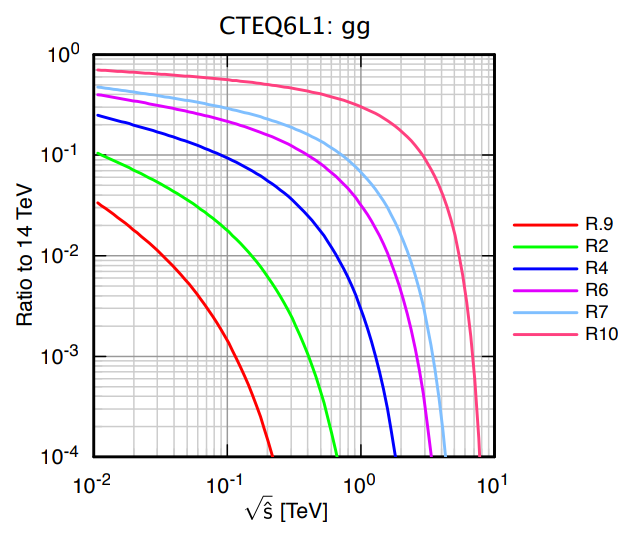
\includegraphics[width=0.5\textwidth]{figures/pheno/partonLumi.png}
\caption{Comparison of $gg$ luminosity for different \sqrts, plotted as a ratio to the luminosity at \sqrts=14~TeV. Figure from \cite{quigg}.}
\label{fig:partonLumi}
\end{figure}

The luminosity defined in Equation \ref{eqn:lumi} is defined in terms of the $pp$ cross section $\sigma_{pp}$.
A more specific \emph{parton luminosity} $\mathcal{L}_{ij}$ may be defined for particular species of parton $i$ and $j$ with center-of-mass energy $\sqrths<\sqrts$.
The ``hatted'' variables correspond to values in the partonic center-of-mass frame.
\begin{equation}\begin{split}\label{eqn:partonLumi}
\frac{\tau}{\shat}\frac{d\mathcal{L}_{ij}}{d\tau}\equiv\frac{\tau}{\shat(1+\delta_{ij})} \int_\tau^1 \frac{dx}{x}~f_i(x)f_j(\tau/x)+f_j(x)f_i(\tau/x)]
\end{split}\end{equation}
This definition supposes the beam consists of partons rather than protons, and each parton combination has an associated luminosity that is a function of the fraction $\tau=\shat/s$.
This luminosity depends on the beam energy via the presence of the PDFs and $\feynx$.
The total cross section for $pp\to X$ is defined by with a sum over parton species,
\begin{equation}\begin{split}
\sigma_{pp\to X}(s)=\sum_i\sum_j \frac{d\tau}{\tau}\cdot\frac{\tau}{\shat}\frac{d\mathcal{L}_{ij}}{d\tau}\cdot[\shat\sigma_{ij\to X}(\shat)].
\end{split}\end{equation} 
As indicated by the shapes of PDF curves, the parton luminosity for a beam of energy \sqrts drops off as a function of \sqrths.
\cite{quigg}

Consequently, although the LHC collides beams with \sqrts=13~TeV, the practical luminosity of collisions with \sqrths=13~TeV essentially vanishes.
This limits the energy available in hard scattering to a fraction of \sqrts.
For example, the invariant-mass of the most energetic two-jet event recorded by ATLAS in Run~2 is just $m_{jj}=8$~TeV.
A second consequence of Equation \ref{eqn:partonLumi} arises from its dependence on the proton-proton collision center-of-mass energy \sqrts via $\tau$.
Increasing the \sqrts greatly expands the parton luminosity at large \sqrths.
Both of these effects are illustrated in Figure \ref{fig:partonLumi}, which plots the ratio of $gg$ parton luminosities at the different center-of-mass energies to the LHC design value.

\section{Dilepton Production}\label{sec:phenoBkg}

Both the \hmm and non-resonant analyses measure the dilepton invariant-mass spectra to search for a signal.
As such, the backgrounds for these analyses share a similar composition predicted by the SM.
The dominant hard-scattering processes that produce events with dilepton pairs in the high invariant-mass region at the LHC are described in this section.

\begin{figure}[h!]
\captionsetup[subfigure]{position=b}
\centering
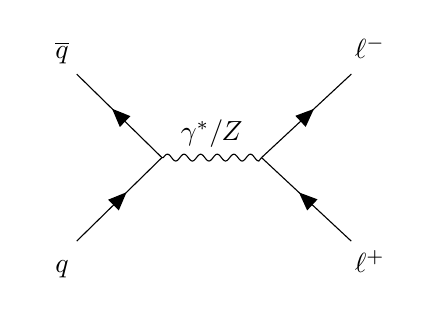
\begin{tikzpicture}\begin{feynman}[medium]
    \vertex (p1);
    \vertex [right=3.6em of p1] (p2);
    \vertex [above left=of p1] (qa){\(\phantom{^+}\qbar\)};
    \vertex [below left=of p1] (qb){\(\phantom{^+}q\)};
    \vertex [above right=of p2] (h){\(\ell^{-}\phantom{\qbar}\)};
    \vertex [below right=of p2] (v){\(\ell^{+}\phantom{\qbar}\)};
    \diagram* {
    (qb) --[fermion] (p1) --[fermion] (qa),
    (p1) --[boson,edge label=\(\gamma^*/Z\)] (p2),
    (v) --[fermion] (p2) --[fermion] (h),
    };
\end{feynman}
\end{tikzpicture}
    % \feynmandiagram [medium,baseline=(v1.base),horizontal=v1 to v2] {
    % q1[particle=\(q\)] --[fermion] v1 --[boson,edge label=\(\gamma^*/Z\)] v2 --[fermion] z1[particle=\(\ell^-\)],
    % v1 --[fermion] q2[particle=\(\overline{q}\)],
    % z2[particle=\(\ell^+\)] --[fermion]v2,
    % }; \\ [1em]
\caption{Feynman diagram for the leading order Drell-Yan process.}
\label{fig:phenoDy}
\end{figure}

The most significant lepton pair production mechanism in hadronic collisions was proposed in 1970 by Sidney Drell and Tung-Mow Yan. 
The process is described as the annihilation of quark-antiquark pairs from opposing protons to produce a massive intermediate state that carries the momentum exchange of the collision \cite{drellYan}.
For collision energies below the \Z mass, this intermediate state is an off-shell photon.
Above the \Z mass, both photons and \Z bosons mediate Drell-Yan production, as illustrated in Figure \ref{fig:phenoDy}.
The predicted differential cross-section falls sharply as the produced dilepton pair's invariant mass grows.
Although this prediction is inaccurate near the \Z mass where resonant production dominates, in the kinematic regions of interest for this thesis, it describes the background to the first order.


\begin{figure}[h!]
\captionsetup[subfigure]{position=b}
\centering
\subfloat[]{\raisebox{1.3ex}{
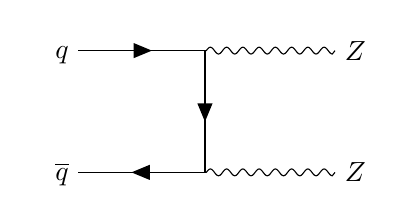
\begin{tikzpicture}\begin{feynman}[medium]
    \vertex(qa) {\(\phantom{^+}q\)};
    \vertex [below=4.4em of qa] (qb){\(\phantom{^+}\qbar\)};
    \vertex [right=5.5em of qa] (p1);
    \vertex [right=4.7em of p1] (z1){\(Z\)};
    \vertex [right=5.5em of qb] (p2);
    \vertex [right=4.7em of p2] (z2){\(Z\)};
    \diagram* {
    (qa) --[fermion] (p1) --[fermion] (p2) --[fermion] (qb),
    (p1) --[boson] (z1),
    (p2) --[boson] (z2),
    };
\end{feynman}
\end{tikzpicture}
}}
\subfloat[][]{{
    \feynmandiagram [medium,baseline=(v1.base),horizontal=v1 to v2] {
    q1[particle=\(q\)] --[fermion] v1 --[boson,edge label=\(W\)] v2 --[boson] z1[particle=\(Z\phantom{^+}\)],
    v1 --[fermion] q2[particle=\(\qbar'\)],
    v2 --[boson] z2[particle=\(W\phantom{^+}\)],
    };
}}
\subfloat[][]{{
    \feynmandiagram [medium,baseline=(v1.base),horizontal=v1 to v2] {
    q1[particle=\(q\)] --[fermion] v1 --[boson,edge label=\(Z\)] v2 --[boson] z1[particle=\(W^-\)],
    v1 --[fermion] q2[particle=\(\qbar\phantom{'}\)],
    v2 --[boson] z2[particle=\(W^+\)],
    };
}}
\caption{Representative Feynman diagrams for leading order diboson production for ZZ (a) WZ (b) and WW (c).}
\label{fig:phenoDiboson}
\end{figure}


% \begin{figure}[h!]
% \captionsetup[subfigure]{position=b}
% \centering
% \subfloat[][]{{
%     \feynmandiagram [medium,baseline=(v1.base),vertical=v2 to v1] {
%     b[particle=\(q\)] --[fermion] v2,
%     v2 --[boson] t[particle=\(Z\)],
%     v1 --[boson] qb[particle=\(Z\)],
%     v1 --[fermion] qa[particle=\(\overline{q}'\)],
%     v2 --[fermion] v1,
%     };
% }}
% \hspace{2em}
% \subfloat[][]{{
%     \feynmandiagram [medium,baseline=(v1.base),horizontal=v1 to v2] {
%     q1[particle=\(q\)] --[fermion] v1 --[boson,edge label=\(W\)] v2 --[boson] z1[particle=\(Z\)],
%     v1 --[fermion] q2[particle=\(\overline{q}'\)],
%     v2 --[boson] z2[particle=\(W\)],
%     };
% }}
% \subfloat[][]{{
%     \feynmandiagram [medium,baseline=(v1.base),horizontal=v1 to v2] {
%     q1[particle=\(q\)] --[fermion] v1 --[boson,edge label=\(Z\)] v2 --[boson] z1[particle=\(W^-\)],
%     v1 --[fermion] q2[particle=\(\overline{q}\)],
%     v2 --[boson] z2[particle=\(W^+\)],
%     };
% }}
% \caption{Representative Feynman diagrams for leading order diboson production for ZZ (a) WZ (b) and WW (c).}
% \label{fig:phenoDiboson}
% \end{figure}

The next leading source of dilepton events come from \emph{diboson} production.
These are described by diagrams, including those in Figure \ref{fig:phenoDiboson}, with two vector bosons \W or \Z in their final state.
The leading order production of these events is through the $q\qbar$ initial state.

\begin{figure}[h!]
\captionsetup[subfigure]{position=b}
\centering
\subfloat[][]{{
    \feynmandiagram [medium,baseline=(v1.base),horizontal=v1 to v2] {
    b[particle=\(g\)] --[gluon] v1  --[gluon] v2,
    v2 --[fermion] t[particle=\(t\)],
    qa[particle=\(g\)]--[gluon]v1,
    qb[particle=\(\overline{t}\)]--[fermion]v2,
    };
}}
\hspace{2em}
\subfloat[]{\raisebox{1.6ex}{
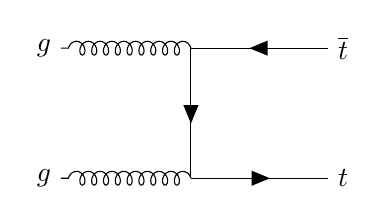
\begin{tikzpicture}\begin{feynman}[medium]
    \vertex(qa) {\(\tbar\)};
    \vertex [below=4.7em of qa] (qb){\(t\)};
    \vertex [left=5.5em of qa] (p1); 
    \vertex [left=4.7em of p1] (g1){\(g\)}; 
    \vertex [left=5.5em of qb] (p2); 
    \vertex [left=4.7em of p2] (g2){\(g\)}; 
    \diagram* {
    (qa) --[fermion] (p1) --[fermion] (p2) --[fermion] (qb),
    (p1) --[gluon] (g1),
    (p2) --[gluon] (g2),
    };
\end{feynman}
\end{tikzpicture} 
}}
\hspace{2em}
\subfloat[][]{{
    \feynmandiagram [medium,baseline=(v1.base),horizontal=v1 to v2] {
    b[particle=\(q\)] --[fermion] v1  --[gluon] v2,
    v2 --[fermion] t[particle=\(t\)],
    v1--[fermion]qa[particle=\(\overline{q}\)],
    qb[particle=\(\overline{t}\)]--[fermion]v2,
    };
}}
\caption{Representative Feynman diagrams for leading order $t\tbar$ production.}
\label{fig:phenoTtbar}
\end{figure}

% \begin{figure}[h!]
% \captionsetup[subfigure]{position=b}
% \centering
% \subfloat[][]{{
%     \feynmandiagram [medium,baseline=(v1.base),horizontal=v1 to v2] {
%     b[particle=\(g\)] --[gluon] v1  --[gluon] v2,
%     v2 --[fermion] t[particle=\(t\)],
%     qa[particle=\(g\)]--[gluon]v1,
%     qb[particle=\(\overline{t}\)]--[fermion]v2,
%     };
% }}
% \hspace{2em}
% \subfloat[][]{{
%     \feynmandiagram [medium,baseline=(v1.base),vertical=v1 to v2] {
%     g1[particle=\(g\)] --[gluon] v1,
%     t1[particle=\(\overline{t}\)] --[fermion]v1,
%     g2[particle=\(g\)] --[gluon] v2 --[fermion] t2[particle=\(t\)],
%     v1 --[fermion] v2,
%     };
% }}
% \hspace{2em}
% \subfloat[][]{{
%     \feynmandiagram [medium,baseline=(v1.base),horizontal=v1 to v2] {
%     b[particle=\(q\)] --[fermion] v1  --[gluon] v2,
%     v2 --[fermion] t[particle=\(t\)],
%     v1--[fermion]qa[particle=\(\overline{q}\)],
%     qb[particle=\(\overline{t}\)]--[fermion]v2,
%     };
% }}
% \caption{Representative Feynman diagrams for leading order $t\tbar$ production.}
% \label{fig:phenoTtbar}
% \end{figure}

\begin{figure}[h!]
\captionsetup[subfigure]{position=b}
\centering
\subfloat[][]{{
    \feynmandiagram [small,baseline=(v1.base),horizontal=qa to qb] {b[particle=\(\phantom{'}q\)] --[fermion] v2 --[fermion] t[particle=\(q'\)],qa[particle=\(\phantom{'}b\)] --[fermion] v1 --[fermion] qb[particle=\(t\phantom{'}\)],v2 --[boson] v1};
}}
\hspace{2em}
\subfloat[]{\raisebox{3.6em}{
    \feynmandiagram [small,baseline=(v1.base),horizontal=v1 to v2] {
    b[particle=\(q\)] --[fermion] v1  --[boson,edge label=\(W\)] v2,
    v2 --[fermion] t[particle=\(t\phantom{'}\)],
    v1--[fermion]qa[particle=\(\qbar'\)],
    qb[particle=\(\bbar\phantom{'}\)]--[fermion]v2,
    };
}}
\hspace{2em}
\subfloat[]{\raisebox{3.6em}{
    \feynmandiagram [small,baseline=(v1.base),horizontal=v1 to v2] {
    b[particle=\(\phantom{'}g\)] --[gluon] v1  --[fermion] v2,
    v2 --[fermion] t[particle=\(t\phantom{'}\)],
    qa[particle=\(\phantom{'}b\)]--[fermion]v1,
    qb[particle=\(W\phantom{'}\)]--[boson]v2,
    };
}}
\hspace{2em}
\subfloat[][]{{
    \feynmandiagram [small,baseline=(v1.base),vertical=v1 to v2] {
    b[particle=\(\phantom{'}b\)] --[fermion] v1 --[boson] w[particle=\(W\phantom{'}\)],
    g[particle=\(\phantom{'}g\)] --[gluon] v2 --[fermion] t[particle=\(t\phantom{'}\)],
    v1 --[fermion] v2,
    };
}}
\caption{Representative Feynman diagrams for leading order single-top production. Subfigures (a) and (b) show $s$-channel and $t$-channel diagrams respectively. Subfigures (c) and (d) show the leading order $bg\to Wt$ diagrams.}
\label{fig:phenoSingleTop}
\end{figure}

% \begin{figure}[h!]
% \captionsetup[subfigure]{position=b}
% \centering
% \subfloat[][]{{
%     \feynmandiagram [small,baseline=(v1.base),horizontal=qa to qb] {b[particle=\(q\)] --[fermion] v2 --[fermion] t[particle=\(q'\)],qa[particle=\(b\)] --[fermion] v1 --[fermion] qb[particle=\(t\)],v2 --[boson] v1};
% }}
% \hspace{2em}
% \subfloat[][]{{
%     \feynmandiagram [small,baseline=(v1.base),horizontal=v1 to v2] {
%     b[particle=\(q\)] --[fermion] v1  --[boson,edge label=\(W\)] v2,
%     v2 --[fermion] t[particle=\(t\)],
%     v1--[fermion]qa[particle=\(\overline{q}'\)],
%     qb[particle=\(\overline{b}\)]--[fermion]v2,
%     };
% }}
% \hspace{2em}
% \subfloat[][]{{
%     \feynmandiagram [small,baseline=(v1.base),horizontal=v1 to v2] {
%     b[particle=\(g\)] --[gluon] v1  --[fermion] v2,
%     v2 --[fermion] t[particle=\(t\)],
%     qa[particle=\(b\)]--[fermion]v1,
%     qb[particle=\(W\)]--[boson]v2,
%     };
% }}
% \hspace{2em}
% \subfloat[][]{{
%     \feynmandiagram [small,baseline=(v1.base),vertical=v1 to v2] {
%     b[particle=\(b\)] --[fermion] v1 --[boson] w[particle=\(W\)],
%     g[particle=\(g\)] --[gluon] v2 --[fermion] t[particle=\(t\)],
%     v1 --[fermion] v2,
%     };
% }}
% \caption{Representative Feynman diagrams for leading order single-top production. Subfigures (a) and (b) show $s$-channel and $t$-channel diagrams respectively. Subfigures (c) and (d) show the leading order $bg\to Wt$ diagrams.}
% \label{fig:phenoSingleTop}
% \end{figure}

Figure \ref{fig:phenoTtbar} shows diagrams for the production of pairs of top quarks: $t\tbar$.
The leading order diagrams produce top quarks through interactions with gluons.
Figure \ref{fig:phenoSingleTop} shows diagrams for single-top production.
This primarily takes place through production with a lighter quark.
At the LHC, the $t$-channel production shown in Figure \ref{fig:phenoSingleTop} (b) is most prevalent, since the $s$-channel diagram requires a bottom quark initial state \cite{Kidonakis:2011wy}.
Additional production exists in conjunction with a \W boson, which also requires an initial state bottom quark \cite{Kidonakis:2010ux}.
After being produced, the top quarks rapidly decay to a \W and lighter quark (bottom, strange, or down) final state.
Most ($96\pm3\%$) top quarks decay to a final state with a bottom quark \cite{pdg2018}.
The result is, in some cases, a final state with multiple leptons.

\cite{Kidonakis:2011wy, Kidonakis:2010ux}



% \afterpage{
% \begin{table}[htp]
% \begin{center}
% \begin{tabular}{C{0.3\textwidth} C{0.5\textwidth}}
% \toprule
% Process & Diagram \\
% \midrule
% Drell-Yan & 
%     \feynmandiagram [medium,baseline=(v1.base),horizontal=v1 to v2] {
%     q1[particle=\(q\)] --[fermion] v1 --[boson,edge label=\(\gamma^*/Z\)] v2 --[fermion] z1[particle=\(\ell^-\)],
%     v1 --[fermion] q2[particle=\(\overline{q}\)],
%     z2[particle=\(\ell^+\)] --[fermion]v2,
%     }; \\ [1em]
% Diboson &
%     \feynmandiagram [medium,baseline=(v1.base),horizontal=v1 to v2] {
%     q1[particle=\(q\)] --[fermion] v1 --[boson] v2 --[boson] z1[],
%     v1 --[fermion] q2[particle=\(\overline{q}'\)],
%     v2 --[boson] z2[],
%     }; \\ [1em]
% Single-top & 
%     \feynmandiagram [medium,baseline=(v1.base),horizontal=v1 to v2] {
%     b[particle=\(q\)] --[fermion] v1  --[boson,edge label=\(W\)] v2,
%     v2 --[fermion] t[particle=\(\overline{t}\)],
%     v1--[fermion]qa[particle=\(\overline{q}'\)],
%     qb[particle=\(b\)]--[fermion]v2,
%     }; \\ [1em]
% Wt & 
%     \feynmandiagram [medium,baseline=(v1.base),horizontal=v1 to v2] {
%     b[particle=\(g\)] --[gluon] v1  --[fermion] v2,
%     v2 --[fermion] t[particle=\(t\)],
%     qa[particle=\(b\)]--[fermion]v1,
%     qb[particle=\(W\)]--[boson]v2,
%     }; \\ [1em]
% $t\tbar$ &
%     \feynmandiagram [medium,baseline=(v1.base),horizontal=v1 to v2] {
%     b[particle=\(g\)] --[gluon] v1  --[gluon] v2,
%     v2 --[fermion] t[particle=\(t\)],
%     qa[particle=\(b\)]--[gluon]v1,
%     qb[particle=\(t\)]--[fermion]v2,
%     }; \\
% \bottomrule
% \end{tabular}
% \caption{Representative Feynman diagrams for the leading background processes for dilepton events at the LHC. In several cases additional diagrams contribute at leading order. These will be specified in more detail in the context in which they are relevant.}
% \label{tab:phenoBkg}
% \end{center}
% \end{table}
% \clearpage
% }

\section{Higgs Production Mechanisms}\label{sec:phenoHiggs}

\begin{figure}[h!]
\captionsetup[subfigure]{position=b}
\centering
\subfloat[][]{\label{fig:higgsCrossSection}{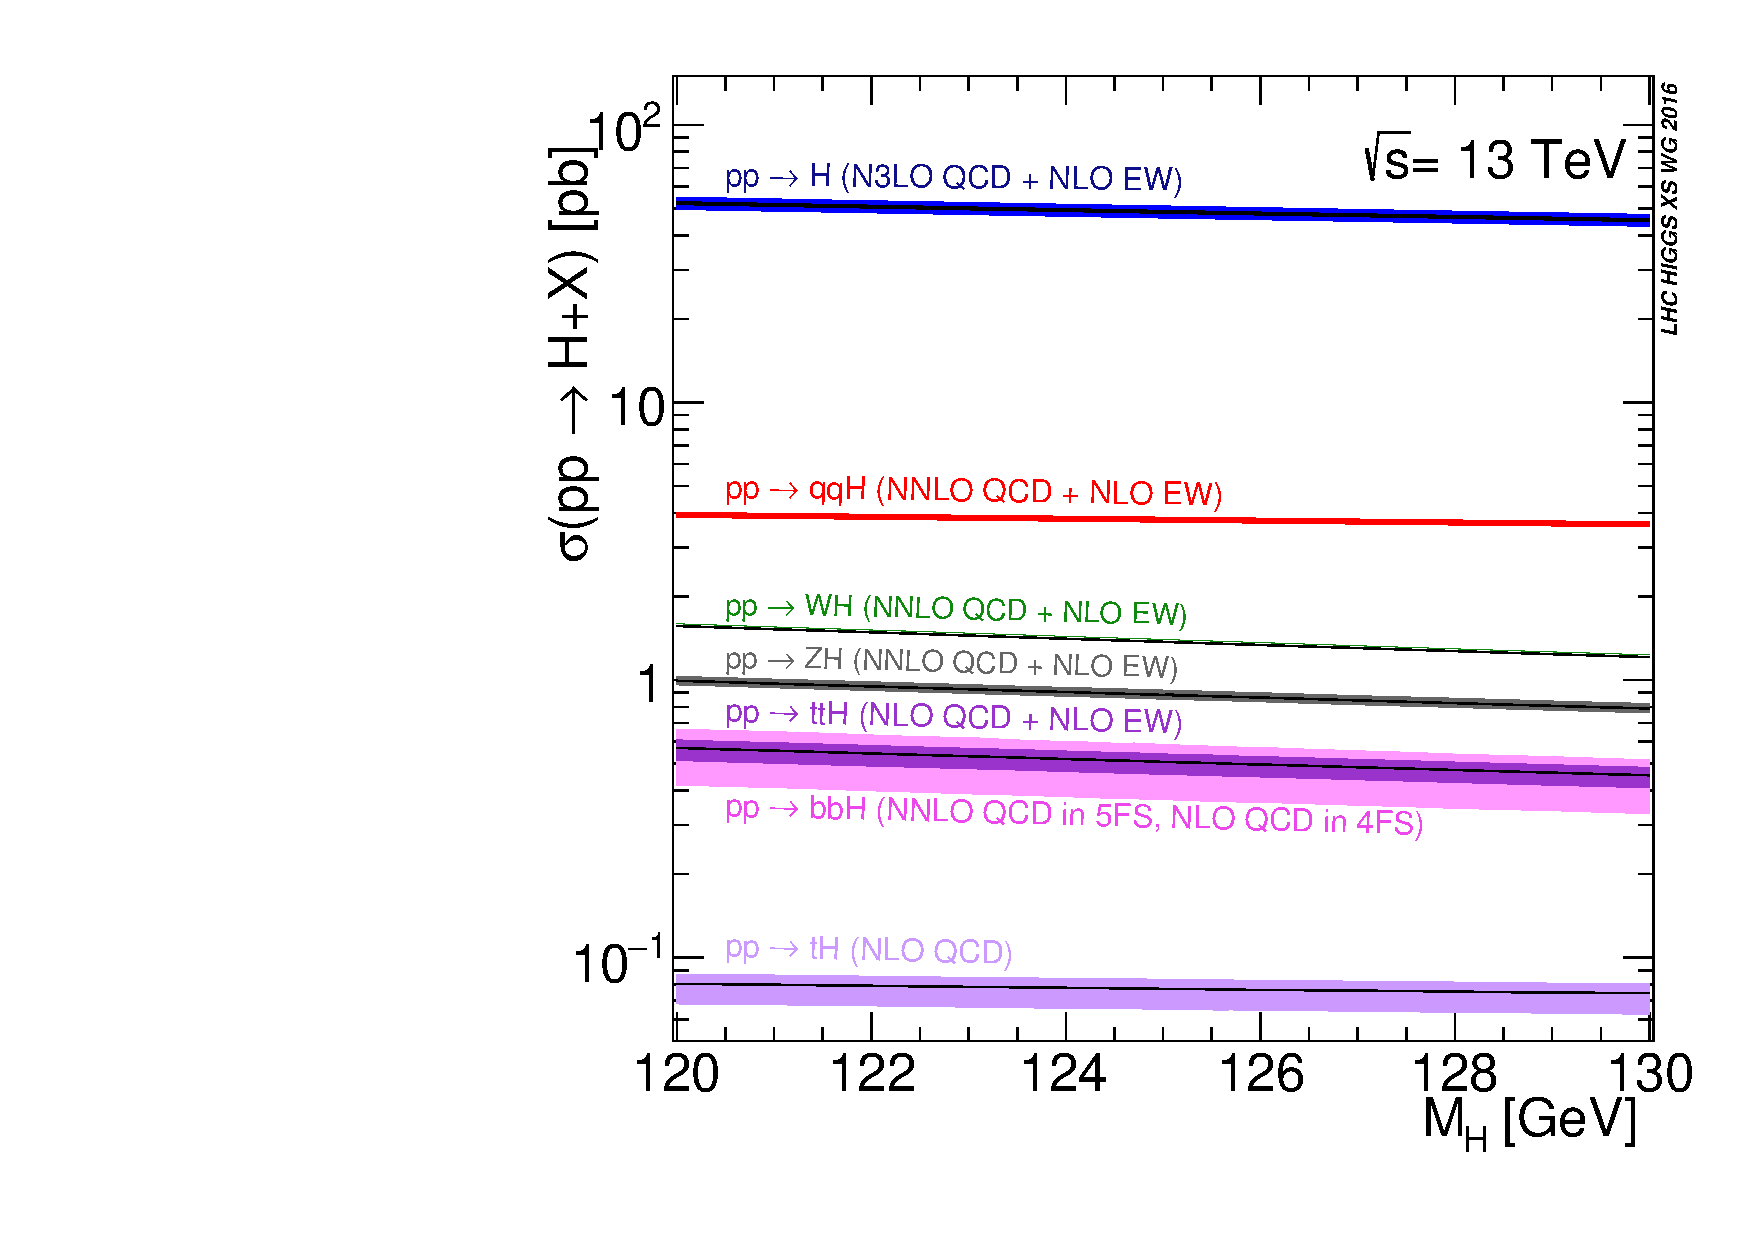
\includegraphics[width=0.5\textwidth]{figures/pheno/higgsXsec-mh.pdf}}}
\subfloat[][]{{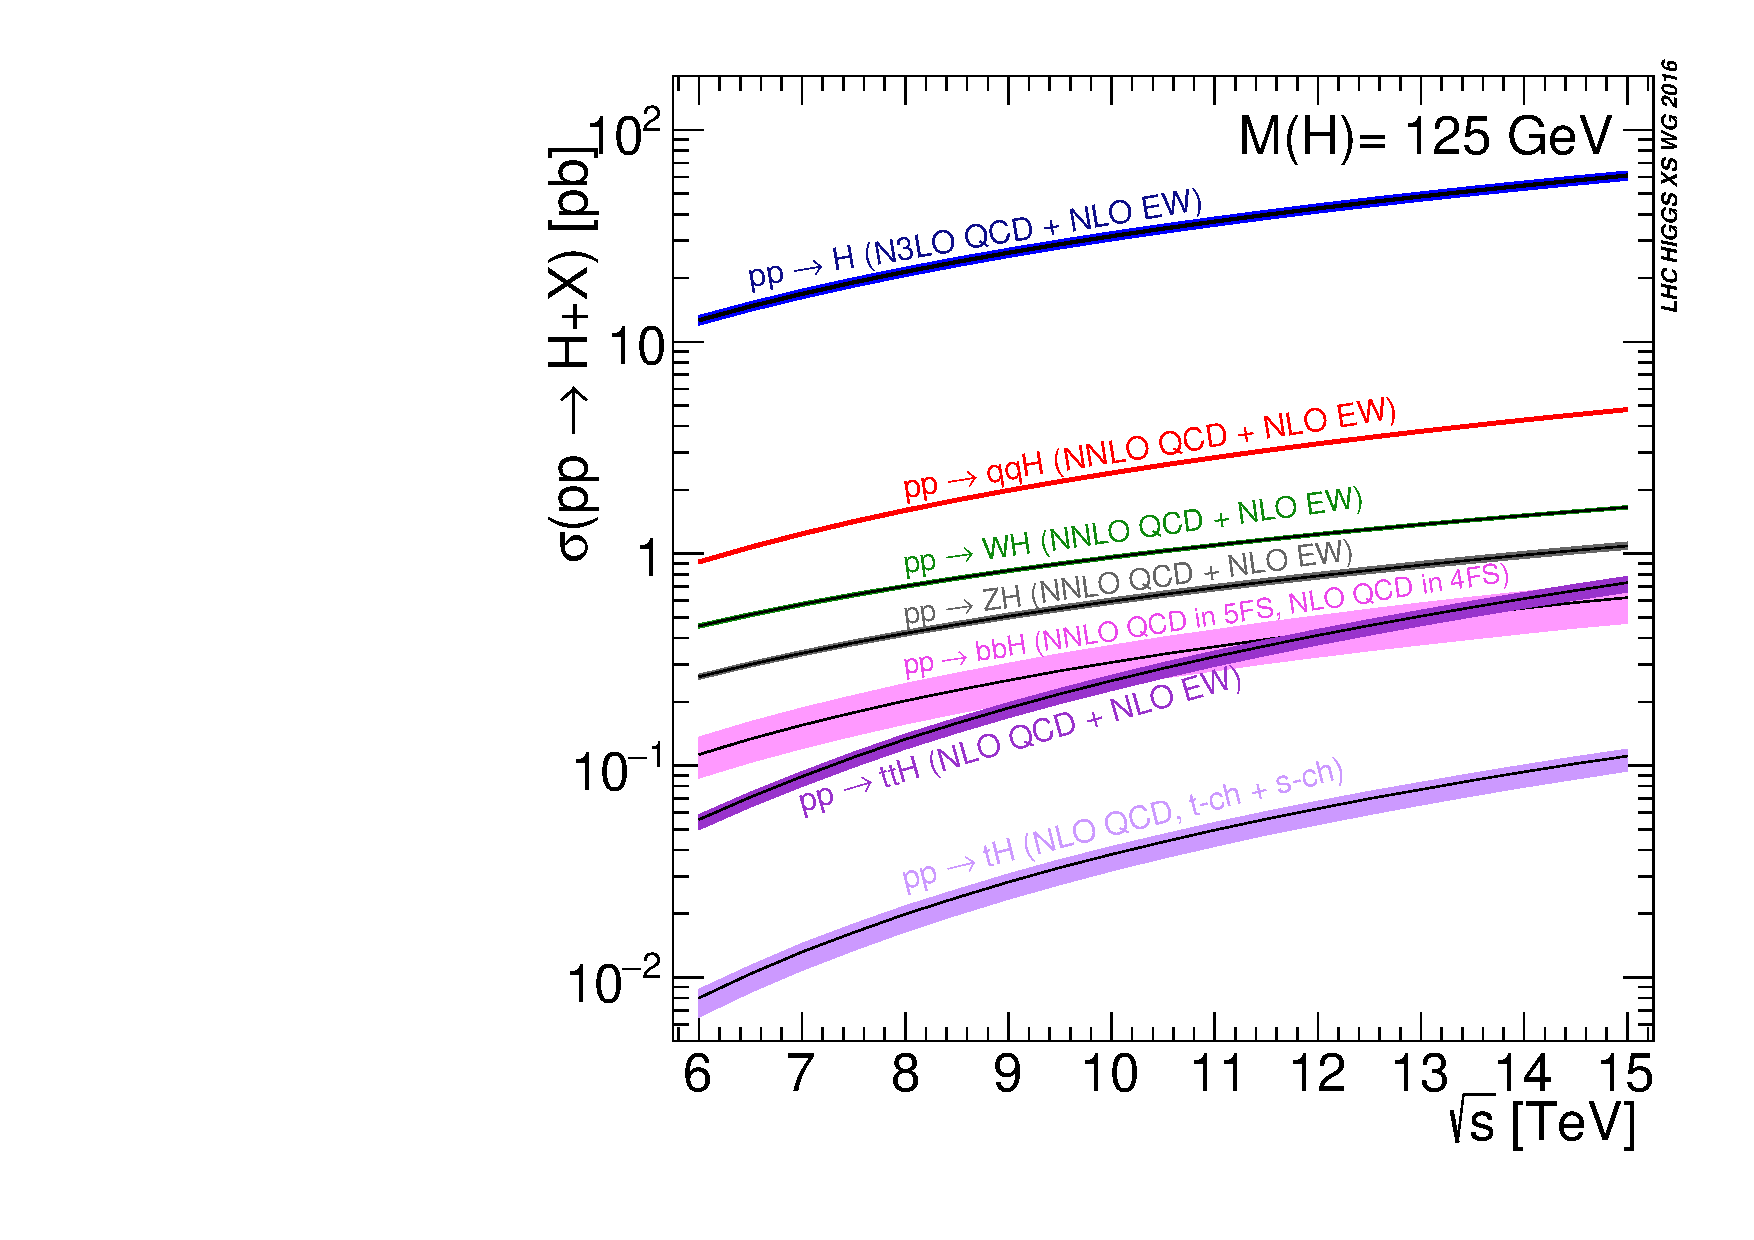
\includegraphics[width=0.5\textwidth]{figures/pheno/higgsXsec-s.pdf}}}
\label{fig:}
\caption{The cross sections of various Higgs production mechanisms shown as a function of (a) Higgs mass and (b) \sqrts.}
\end{figure}


The total production cross-section for Higgs bosons at in $\sqrts=13$~TeV proton-proton collisions at the LHC is 55.7~pb \cite{higgsCross}.
\footnote{This cross-section is calculated to N3LO precision, which calculates contributions from processes represented by Feynman diagrams that include up to three loops.}
Higgs bosons are produced through several distinct mechanisms at the LHC.
These are distinguished by both their initial states and the topology of their final states.
The leading production process, responsible for 89\% of all Higgs, is through gluon-gluon fusion (ggF).
Although there is no direct coupling between gluons and the Higgs, the interaction is mediated by a quark loop.
The large coupling of the Higgs to the top quark means this loop is primarily composed of top quarks.
The next leading production mechanism is vector boson fusion (VBF), with roughly 9\% of the cross-section as ggF.
In this process, the Higgs is produced through a ``collision'' of either \W or \Z bosons that are radiated from the initial state quarks.
The final state includes the Higgs, along with two quarks that rapidly hadronize to form jets.
The presence of two jets in the final state help distinguish VBF events from background processes and ameliorates the challenge of its low cross-section.
The weakest production mechanisms are ttH and bbH, where the Higgs is produced in conjunction with a top or bottom quark pair.

The production mechanisms with the third-largest cross-section are collectively called ``Higgs produced in association with a vector boson'', or VH.
These are the primary focus for the \hmm search presented in this thesis.
There are several ``sub-mechanisms'' that contribute to VH.
Of these, the one with the largest cross-section is the s-channel production with initial state quarks whimsically called \emph{Higgs-strahlung} in analogy to Bremsstrahlung radiation.
When the mediator boson is a \W, then Higgs-strahlung is responsible for the leading order WH production mechanism.
As a result of the corresponding parton luminosities, the cross-section of WH depends on the charge of the mediating $W$ boson: the production positively charged \Wp benefits from the enhanced PDF of valance $u$-quarks seen in Figure \ref{fig:partonLumi}. 
The cross section for WH production is given in Equation \ref{eqn:whxs}.

\begin{equation}\begin{split}\label{eqn:whxs}
\sigma(q_i\qbar_j\to WH)=\frac{\pi\alpha^2 |V_{ij}|^2}{36 \sin^4\theta_W} \frac{2k}{\sqrts} \frac{k^2+3m^2_W}{(s-m^2_W)^2}
\end{split}\end{equation} 
Here $V_{ij}$ are the CKM matrix elements, $k$ is the center-of-mass momentum of the Higgs, and $\theta_W$ is the Weinberg angle defined in Section \ref{sec:ewTheory}.

When the mediator boson is a \Z, then Higgs-strahlung is the leading production mechanism for ZH as well.
The cross section for ZH production in $pp$ collisions is given in Equation \ref{eqn:zhxs}.
\begin{equation}\begin{split}\label{eqn:zhxs}
\sigma(f\overline{f}\to ZH)=\frac{\pi\alpha^2 \ell_f^2r_f^2}{48N_c\sin^4\theta_W\cos^4\theta_W} \frac{2k}{\sqrts} \frac{k^2+3m^2_Z}{(s-m^2_Z)^2}
\end{split}\end{equation} 
Here, $r\equiv-2Qx_W$, $\ell\equiv2(T_3-Qx_W$,
$T_3$ is the third component of weak isospin for the left-handed $f$, $Q^2$ is its electric charge, and $x_W\equiv\sin^2\theta_W$.
While Equation \ref{eqn:zhxs} describes the $q\qbar\to ZH$ cross-section, it is also applicable to $\ell^+\ell^-$ collisions that might take place in future lepton colliders.
This makes this process of particular interest for precision measurements of Higgs properties in, for example, future $e^+e^-$ colliders.

Unlike with WH production, the sub-leading mechanisms are not negligible for ZH production.
These consist of interactions with two initial state gluons where the Higgs is produced via a heavy quark loop.
There are two diagrams to consider: a ``box'' diagram and a ``triangle'' diagram.
Together, these represent $\approx10\%$ of the total ZH production cross-section.

\begin{table}[htp]
\caption{Vector boson leptonic decays include $\tau$. Higgs mass at 125 GeV \cite{higgsCross}.}
\begin{center}
{\footnotesize
\begin{tabular}{l | l | l l l}
\toprule
Production & Cross section [pb] & Uncertainty (theory) [\%] & Uncertainty (PDF/$\alpha_s$) [\%] \\
\midrule
Gluon-gluon fusion (ggF)  & 48.6        & +4.6, -6.7 & $\pm3.9$  \\
Vector boson fusion (VBF) &  3.78       & +0.5, -0.3 & $\pm2.1$  \\
Associated W (WH)         & 1.37        & +0.4, -0.7 & $\pm1.8$  \\
$\hookrightarrow$  $\Wp\to\ell^+\nu$    &$\hookrightarrow$ 0.0943 &$\hookrightarrow$ +0.5, -0.7 &$\hookrightarrow$ $\pm1.8$  \\
$\hookrightarrow$  $\Wm\to\ell^-\nu$    &$\hookrightarrow$ 0.0583  &$\hookrightarrow$ +0.4, -0.7 &$\hookrightarrow$ $\pm2.0$  \\
Associated Z (ZH)         & 0.839       & +3.8, -3.1 & $\pm1.6$  \\
$\hookrightarrow$  $Z\to\ell^+\ell^-$   &$\hookrightarrow$ 0.0298 &$\hookrightarrow$ +3.8, -3.1 &$\hookrightarrow$ $\pm1.6$  \\
ttH                       &  0.507      & +5.8, -9.2 & $\pm3.6$  \\
\bottomrule
\end{tabular}
}
\label{tab:higgsCrossSec}
\end{center}
\end{table}

The diagrams for VH processes, along with the other leading production mechanisms, are shown in Table \ref{tab:higgsProdDiagrams}.
The cross-sections and the associated theoretical uncertainties, are given in Table \ref{tab:higgsCrossSec}.
As mentioned earlier, these cross sections depend on the Higgs mass. The Numbers in Table \ref{tab:higgsCrossSec} are calculated with \mh=125~GeV, and the functional dependence is shown in Figure \ref{fig:higgsCrossSection}.

\begin{table}[p!]
\caption{The leading order Feynman diagrams for the dominant Higgs production mechanisms at the LHC. Together, Higgs-strahlung and the two ZH diagrams comprise VH.}
\begin{center}
{
\begin{tabular}{C{0.3\textwidth} C{0.5\textwidth}}
\toprule
Higgs Production & Diagram \\
\midrule
\centered{Gluon-gluon fusion}  &
\centered{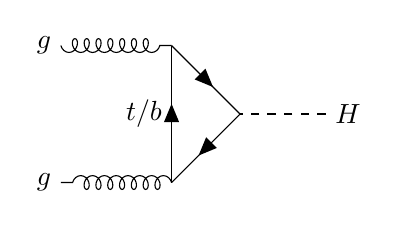
\begin{tikzpicture}
\begin{feynman}
    \vertex (h){\(H\)};
    \vertex [left=3.9em of h] (v);
    \vertex [above left= 3.5em of v] (p1);
    \vertex [below left= 3.5em of v] (p2);
    \vertex [left=4em of p1] (g1){\(g\)};
    \vertex [left=4em of p2] (g2){\(g\)};
    \diagram* {
    (h)[particle=\(H\)] --[scalar] (v),
    (g1)[particle=\(g\)] --[gluon] (p1) --[fermion] (v),
    (v)  --[fermion] (p2) --[gluon] (g2)[particle=\(g\)],
    (p2) --[fermion,edge label=\(t/b\)] (p1),
    };
\end{feynman}
\end{tikzpicture}} \\ [5em]
\centered{Vector boson fusion}  &
\centered{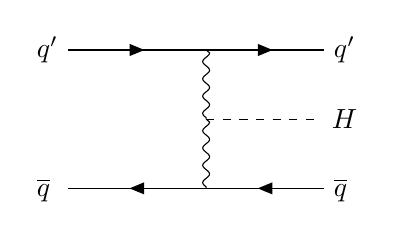
\begin{tikzpicture}
\begin{feynman}
    \vertex (h){\(H\)};
    \vertex [left=5em of h] (p2);
    \vertex [below=2.5em of p2] (p1);
    \vertex [above=2.5em of p2] (p3);
    \vertex [above=2.5em of h] (qbi){\(q'\)};
    \vertex [below=2.5em of h] (qai){\(\qbar\phantom{'}\)};;
    \vertex [left=5em of p3] (qbo){\(q'\)};;
    \vertex [left=5em of p1] (qao){\(\qbar\phantom{'}\)};;
    \diagram* [small,baseline=(h.base),horizontal=p2 to h] {
    (qai) --[fermion] (p1) --[fermion] (qao),
    (qbo) --[fermion] (p3) --[fermion] (qbi),
    (p1) --[boson] (p2) --[boson] (p3),
    (p2) --[scalar] (h),
    };
\end{feynman}
\end{tikzpicture}} \\ [5em]
\centered{Higgs-strahlung ZH/WH}&
\centered{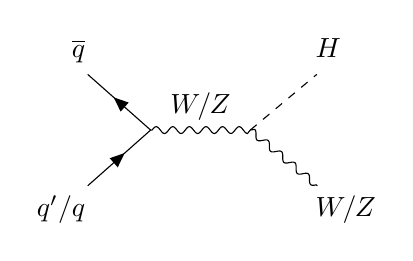
\begin{tikzpicture}\begin{feynman}[small]
    \vertex (p1);
    \vertex [right=3.6em of p1] (p2);
    \vertex [above left=of p1] (qa){\(\phantom{q'/}\qbar\)};
    \vertex [below left=of p1] (qb){\(q'/q\)};
    \vertex [above right=of p2] (h){\(H\phantom{/Z}\)};
    \vertex [below right=of p2] (v){\(W/Z\)};
    \diagram* {
    (qb) --[fermion] (p1) --[fermion] (qa),
    (p1) --[boson,edge label=\(W/Z\)] (p2),
    (v) --[boson] (p2) --[scalar] (h),
    };
\end{feynman}
\end{tikzpicture}} \\ [5em]
\centered{Gluon-originated ZH\\(box diagram)} &
\centered{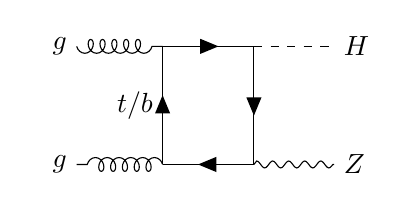
\begin{tikzpicture}
\begin{feynman}
    \vertex (g1){\(\phantom{x}g\)};
    \vertex [right=4.0em of g1](p1);
    \vertex [right=3.3em of p1](p2);
    \vertex [below=of g1](g2){\(\phantom{x}g\)};
    \vertex [right=4.0em of g2](p3);
    \vertex [right=3.3em of p3](p4);
    \vertex [right=2.9em of p2](h){\(H\)};
    \vertex [right=2.9em of p4](z){\(Z\)};
    \diagram* {
    (g1) --[gluon] (p1) --[fermion] (p2) --[scalar] (h),
    (z) --[boson] (p4) --[fermion] (p3) --[gluon] (g2),
    (p3) --[fermion,edge label=\(t/b\)] (p1),
    (p2) --[fermion] (p4),
    };
\end{feynman}
\end{tikzpicture}} \\ [5em]
\centered{Gluon-originated ZH\\(triangle diagram)} &
\centered{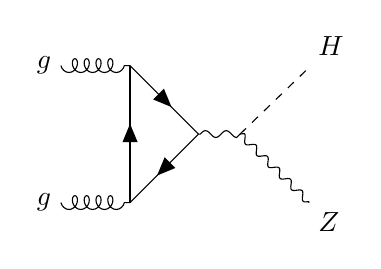
\begin{tikzpicture}
\begin{feynman}
    \vertex (v2);
    \vertex [above right=3.5em of v2](h){\(H\)};
    \vertex [below right=3.5em of v2](z){\(Z\)};
    \vertex [left= 1.5em of v2](v1);
    \vertex [above left= 3.5em of v1](p1);
    \vertex [below left= 3.5em of v1](p3);
    \vertex [left=2.5em of p1](g1){\(g\)};
    \vertex [left=2.5em of p3](g2){\(g\)};
    \diagram* {
    (g1) --[gluon] (p1) --[fermion] (v1) --[boson] (v2) --[scalar] (h),
    (z) --[boson] (v2),
    (v1) --[fermion] (p3),
    (g2) --[gluon] (p3),
    (p3) --[fermion] (p1),
    };
\end{feynman}
\end{tikzpicture}} \\ [5em]
\centered{Top associated production} &
\centered{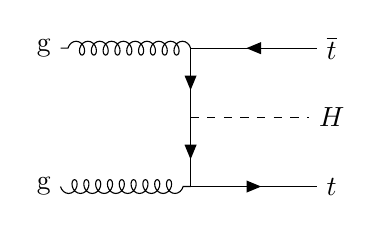
\begin{tikzpicture}
\begin{feynman}
    \vertex (h){\(H\)};
    \vertex [left=5.1em of h] (p2);
    \vertex [above=2.5em of p2] (p1);
    \vertex [below=2.5em of p2] (p3);
    \vertex [above=2.5em of h] (qai){\(\overline{t}\)};;
    \vertex [below=2.5em of h] (qbo){\(t\)};;
    \vertex [left=4.7em of p3] (qbi){g};
    \vertex [left=4.7em of p1] (qao){g};;
    \diagram* [small,baseline=(h.base),horizontal=p2 to h] {
    (qai) --[fermion] (p1) --[gluon] (qao),
    (qbi) --[gluon] (p3) --[fermion] (qbo),
    (p1) --[fermion] (p2) --[fermion] (p3),
    (p2) --[scalar] (h),
    };
\end{feynman}
\end{tikzpicture}} \\ [5em]
\bottomrule
\end{tabular}
}
\label{tab:higgsProdDiagrams}
\end{center}
\end{table}

% \begin{table}[p!]
% \caption{The Feynman diagrams for the leading Higgs production mechanisms at the LHC. Together, Higgs-strahlung and the two ZH diagrams comprise VH.}
% \begin{center}
% {\footnotesize
% \begin{tabular}{C{0.3\textwidth} C{0.5\textwidth}}
% \toprule
% Higgs Production & Diagram \\
% \midrule
% \centered{Gluon-gluon fusion}  &
% \centered{\begin{tikzpicture}
% \begin{feynman}
%     \vertex (h){\(H\)};
%     \vertex [left=of h] (v);
%     \vertex [above left=of v] (p1);
%     \vertex [below left=of v] (p2);
%     \vertex [left=of p1] (g1){\(g\)};
%     \vertex [left=of p2] (g2){\(g\)};
%     \diagram* {
%     (h)[particle=\(H\)] --[scalar] (v),
%     (g1)[particle=\(g\)] --[gluon] (p1) --[fermion] (v),
%     (v)  --[fermion] (p2) --[gluon] (g2)[particle=\(g\)],
%     (p2) --[fermion,edge label=\(t/b\)] (p1),
%     };
% \end{feynman}
% \end{tikzpicture}} \\ [2em]
% \centered{Vector boson fusion}  &
% \centered{\begin{tikzpicture}
% \begin{feynman}
%     \vertex (h){\(H\)};
%     \vertex [left=of h] (p2);
%     \vertex [below=3em of p2] (p1);
%     \vertex [above=3em of p2] (p3);
%     \vertex [above=3em of h] (qbi){\(q'\)};
%     \vertex [below=3em of h] (qai){\(\qbar\)};;
%     \vertex [left=of p3] (qbo){\(q'\)};;
%     \vertex [left=of p1] (qao){\(\qbar\)};;
%     \diagram* [small,baseline=(h.base),horizontal=p2 to h] {
%     (qai) --[fermion] (p1) --[fermion] (qao),
%     (qbo) --[fermion] (p3) --[fermion] (qbi),
%     (p1) --[boson] (p2) --[boson] (p3),
%     (p2) --[scalar] (h),
%     };
% \end{feynman}
% \end{tikzpicture}} \\ [2em]
% \centered{Higgs-strahlung ZH/WH}&
% \centered{\begin{tikzpicture}
% \begin{feynman}
%     \vertex [right=of p1] (p2);
%     \vertex [above left=of p1] (qa){\(\qbar\)};
%     \vertex [below left=of p1] (qb){\(q'/q\)};
%     \vertex [right=of p1] (p2);
%     \vertex [above right=of p2] (h){\(H\)};
%     \vertex [below right=of p2] (v){\(W/Z\)};
%     \diagram* {
%     (qb) --[fermion] (p1) --[fermion] (qa),
%     (p1) --[boson,edge label=\(W/Z\)] (p2),
%     (v) --[boson] (p2) --[scalar] (h),
%     };
% \end{feynman}
% \end{tikzpicture}} \\ [2em]
% \centered{Gluon-originated ZH\\(box diagram)} &
% \centered{\begin{tikzpicture}
% \begin{feynman}
%     \vertex (g1){\(g\)};
%     \vertex [right=of g1](p1);
%     \vertex [right=of p1](p2);
%     \vertex [right=of p2](h){\(H\)};
%     \vertex [below=of g1](g2){\(g\)};
%     \vertex [right=of g2](p3);
%     \vertex [right=of p3](p4);
%     \vertex [right=of p4](z){\(Z\)};
%     \diagram* {
%     (g1) --[gluon] (p1) --[fermion] (p2) --[scalar] (h),
%     (z) --[boson] (p4) --[fermion] (p3) --[gluon] (g2),
%     (p3) --[fermion,edge label=\(t/b\)] (p1),
%     (p2) --[fermion] (p4),
%     };
% \end{feynman}
% \end{tikzpicture}} \\ [2em]
% \centered{Gluon-originated ZH\\(triangle diagram)} &
% \centered{\begin{tikzpicture}
% \begin{feynman}
%     \vertex (v2);
%     \vertex [above right=of v2](h){\(H\)};
%     \vertex [below right=of v2](z){\(Z\)};
%     \vertex [left= 2em of v2](v1);
%     \vertex [above left=of v1](p1);
%     \vertex [below left=of v1](p3);
%     \vertex [left=of p1](g1){\(g\)};
%     \vertex [left=of p3](g2){\(g\)};
%     \diagram* {
%     (g1) --[gluon] (p1) --[fermion] (v1) --[boson] (v2) --[scalar] (h),
%     (z) --[boson] (v2),
%     (v1) --[fermion] (p3),
%     (g2) --[gluon] (p3),
%     (p3) --[fermion] (p1),
%     };
% \end{feynman}
% \end{tikzpicture}} \\ [2em]
% \centered{Top associated production} &
% \centered{\begin{tikzpicture}
% \begin{feynman}
%     \vertex (h){\(H\)};
%     \vertex [left=of h] (p2);
%     \vertex [above=3em of p2] (p1);
%     \vertex [below=3em of p2] (p3);
%     \vertex [left=of p3] (qbi){g};
%     \vertex [above=3em of h] (qai){\(\overline{t}\)};;
%     \vertex [below=3em of h] (qbo){\(t\)};;
%     \vertex [left=of p1] (qao){g};;
%     \diagram* [small,baseline=(h.base),horizontal=p2 to h] {
%     (qai) --[fermion] (p1) --[gluon] (qao),
%     (qbi) --[gluon] (p3) --[fermion] (qbo),
%     (p1) --[fermion] (p2) --[fermion] (p3),
%     (p2) --[scalar] (h),
%     };
% \end{feynman}
% \end{tikzpicture}} \\ [2em]
% \bottomrule
% \end{tabular}
% }
% \label{tab:higgsProdDiagrams}
% \end{center}
% \end{table}

\begin{table}[htp]
\caption{Leptonic decay branching fractions $\Gamma_i/\Gamma$ for \W, \Z, and Higgs \cite{pdg2018}.}
\begin{center}
\begin{tabular}{l r}
\toprule
Decay Mode & BR=$\Gamma_i/\Gamma$ [\%] \\
\midrule
$Z\to e^+e^-$           & $3.36\pm<0.01$ \\
$Z\to \mu^+\mu^-$       & $3.37\pm0.01 $ \\
$W^+\to   e^+\nu_e$     & $10.86\pm0.09$ \\
$W^+\to \mu^+\nu_\mu$   & $10.71\pm0.16$ \\
$H\to \mu^+\mu^-$       & $2.18\times10^{-2}$ (predicted) \\
\bottomrule
\end{tabular}
\label{tab:decayCrossSec}
\end{center}
\end{table}


The partial width of the Higgs boson decaying to two fermions is given by Equation \ref{eqn:higgsDecayFermions}.
\begin{equation}\begin{split}\label{eqn:higgsDecayFermions}
\Gamma(H\to ff)=\frac{G_Fm_f^2m_\text{H}N_c}{4\pi\sqrt{2}}\left(1-4\frac{m_f^2}{m_\text{H}^2}\right)^{3/2}
\end{split}\end{equation} 
Here, the $N_c=1$ for leptons (and 3 for quarks) and $G_F=1.166\times10^{-5}$~GeV$^{-2}$ is the Fermi coupling constant.
The total width, $\Gamma$, is defined as the number of decays per time, per particles present.
It is the sum of all partial widths, such as the fermionic width in Equation \ref{eqn:higgsDecayFermions}.
The total width is equivalent to the reciprocal \emph{lifetime} of the particle $\tau$, which subsequently defines the particle's half-life as $\tau\ln2$.
The partial width also dictates the \emph{branching ratio} that describes the fraction of decays to a particular final state.
For \hmm decays, the branching ratio is therefore

\begin{equation}\begin{split}
    \text{BR}(\hmm)=\frac{\Gamma(\hmm)}{\Gamma}.
\end{split}\end{equation} 

This equation illuminates the central challenge when studying \hmm. 
The total width of the Higgs is expected to be $4.1$~MeV and has been indirectly constrained to be $\Gamma=3.2^{+2.8}_{-2.2}$~MeV \cite{cmsWidth}.
The quadratic dependence on the muon mass $m_f=m_\mu$ in the partial width $\Gamma(\hmm)$ leads to a small branching ratio in the case of the light muon, given in Table \ref{tab:decayCrossSec}.
The partial widths also depend on \mh. This is illustrated in Figure \ref{fig:higgsBr} for the branching ratios, including and larger than \hmm.

\begin{figure}[htb]
\captionsetup[subfigure]{position=b}
\centering
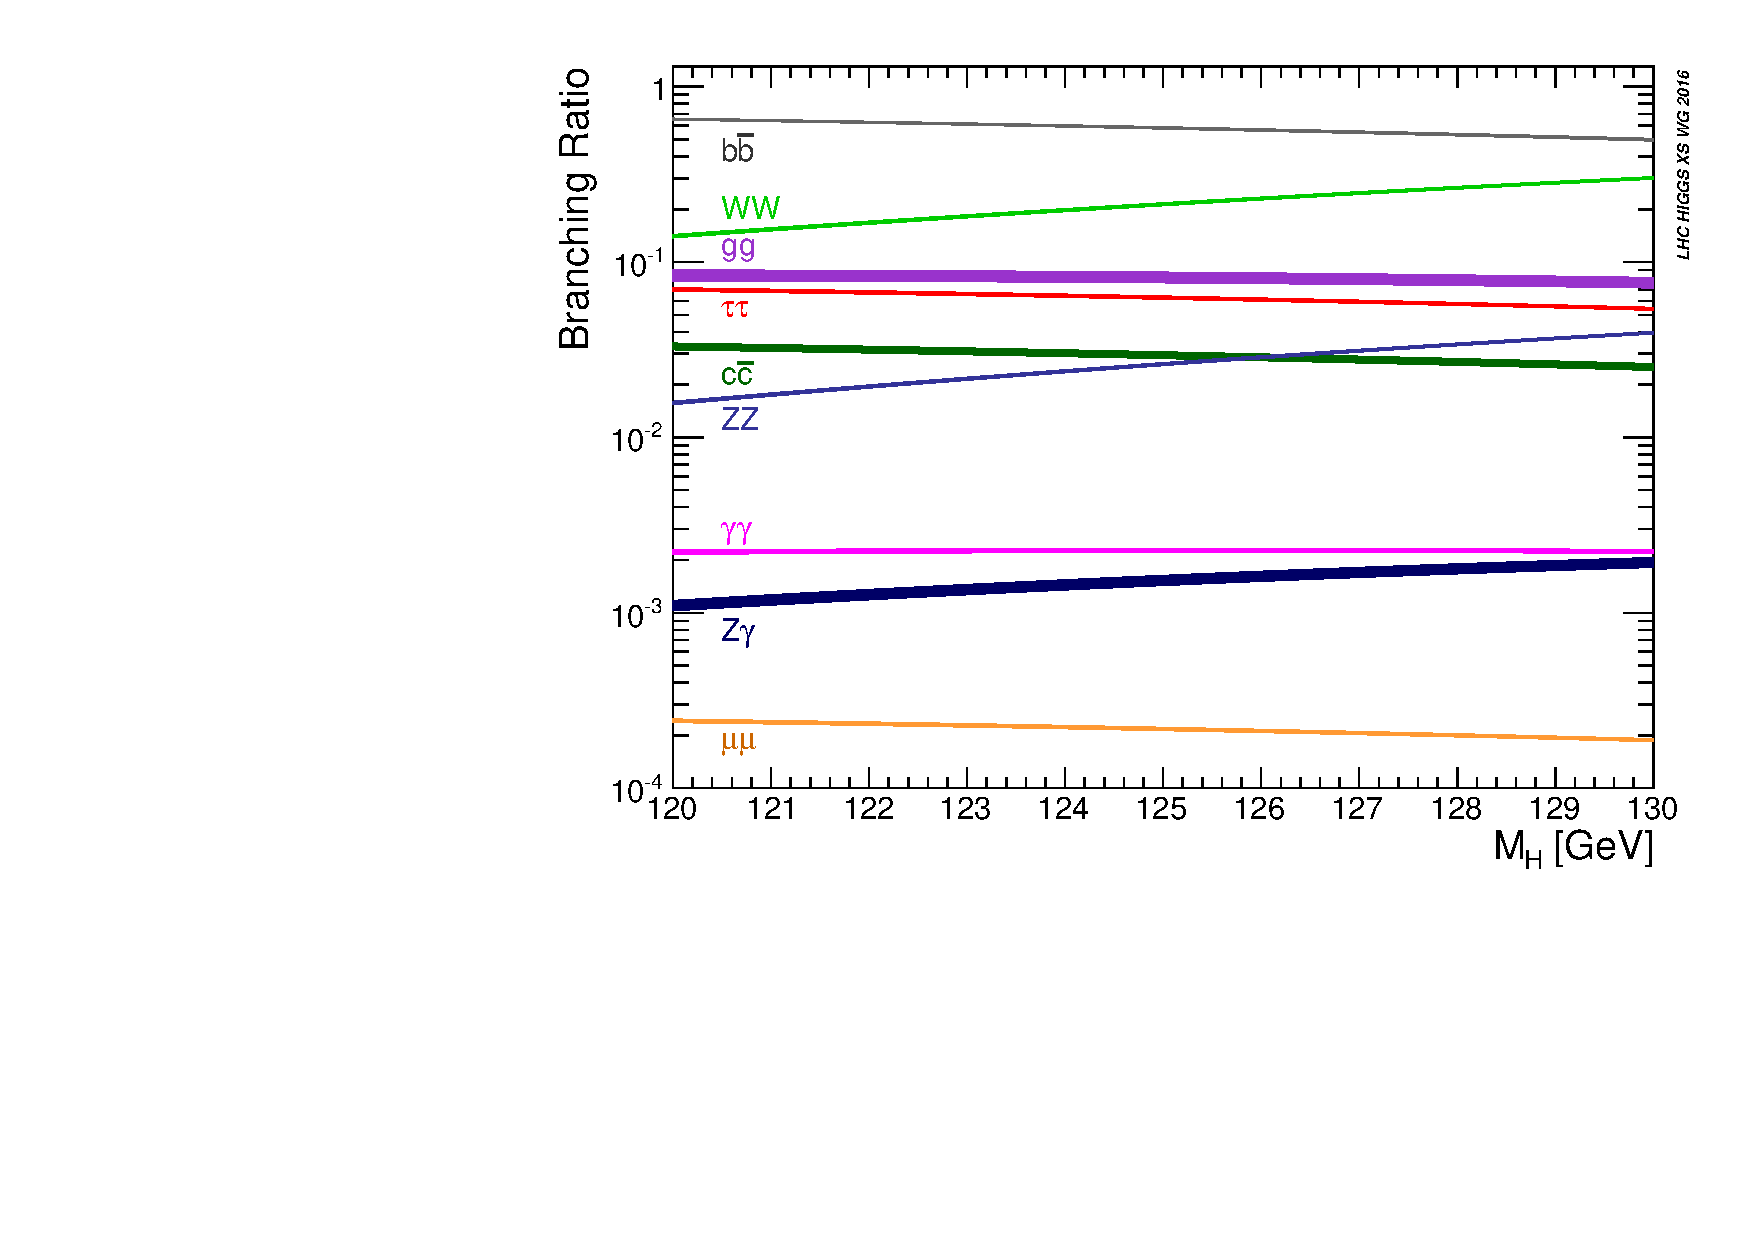
\includegraphics[width=0.5\textwidth]{figures/pheno/higgsBr.pdf}
\caption{Branching ratios of the Higgs boson to several final states as a function of $m_\text{H}$ with $H\to\mu\mu$ shown in yellow at the bottom.}
\label{fig:higgsBr}
\end{figure}

Experimentally, Higgs production and decay to two muons manifests itself in the dimuon invariant-mass spectrum as a resonance above a smoothly falling background.
The resonance width is determined by the total width, $ \Gamma $, by making use of the uncertainty principle in natural units.
A free particle of mass $m$ with some likelihood to decay to a lower energy state can be described by a simple time dependant wave function,
\begin{equation}\begin{split}
    \psi(t)=\psi(0)e^{-imt}e^{-\frac{\Gamma}{2}t}.
\end{split}\end{equation} 
Here, the first exponential represents a stable particle's time evolution, while the second represents the decreasing probability that the particle has not decayed.
The $\Gamma$ is the decay rate and also inverse of the exponential time constant.
The fourier transform of the wave equation describes the particle in energy space,
\begin{equation}\begin{split}
    \psi(E)=\int\psi(t)e^{iEt}dt\propto \frac{1}{(E-m)-i\Gamma/2}.
\end{split}\end{equation}
The energy dependant cross section to observe a decay is proportional to $|\psi(E)|^2$, or 
\begin{equation}\begin{split}\label{eqn:breitWigner}
    \sigma(E)\propto\frac{1}{(E-m)^2+\Gamma^2/4}.
\end{split}\end{equation} 
Equation \ref{eqn:breitWigner} gives the relativistic Breit-Wigner function, which describes resonant features in energy spectra.
The resonance width corresponds to the decay rate; therefore, particles with long lifetimes $\tau$ produce narrow resonances.

These principles determine the phenomenology of \hmm.
The Higgs boson decays with a width $\Gamma$ and the probability distribution of energies described by the Breit-Wigner function.
In \hmm decays, this energy is converted into the dimuon pair's invariant-mass and results in a narrow resonance in the dimuon invariant mass spectrum.
In practice, the energy and momentum resolutions of ATLAS are insufficient to resolve the $\approx4$~MeV width of the Breit-Wigner shape.
Instead, a distribution described approximately a Gaussian function with a width corresponding to the invariant-mass resolution is observed.

% VH leptonic
The final state \W or \Z in a VH event offers an opportunity to help identify Higgs events in the same way that the jets in VBF are useful.
This is particularly true when the \W or \Z decays leptonically since these additional leptons offer a clean signal to help remove events from background production mechanisms.
In the case of \W decays to $\ell^\pm\nu_\ell$ represent $\approx11\%$ of decays for each lepton flavor.
Equation \ref{eqn:wDecayFermions} gives the partial width for leptonic \W decays,
\begin{equation}\begin{split}\label{eqn:wDecayFermions}
    \Gamma(W\to\ell\overline{\nu})=\frac{\sqrt{2}G_Fm_W^3}{12\pi}.
\end{split}\end{equation} 
The total width of the \W boson is $\Gamma=2.085\pm0.042$~GeV.
The leptonic branching fraction is smaller in the case of \Z.
The partial width for \Z decays to fermions is given in Equation \ref{eqn:zDecayFermions}.
\begin{equation}\begin{split}\label{eqn:zDecayFermions}
    \Gamma(Z\to f\fbar)=N_c\frac{\sqrt{2}G_Fm_Z^3}{6\pi}\times[(T_3-Q_f\sin^2\theta_W)^2+(Q_f\sin^2\theta_W)^2]
\end{split}\end{equation} 
The total width of the \Z boson is $\Gamma=2.495\pm0.002$~GeV, and the leptonic width is $\Gamma(\Z\to\ll)=83.984\pm0.086$~MeV per lepton flavor.
The result is a leptonic branching ratio of 3.4\% per flavor \cite{pdg2018}.
The measured values of these branching fractions are given in Table \ref{tab:decayCrossSec}.

\section{Contact Interactions and Compositeness}

Contact interactions are a phenomenological description of new physics interactions above the energy scale accessible directly in collisions.
Such interactions lead to increases in the event rate of high mass events in the dilepton invariant-mass spectra. 
A broad assortment of models predicts such excesses.
Of particular interest are models that propose composite quarks and leptons.
Even within the space of compositeness models, there is great diversity and no consensus about the plausibility of a single model. 
It is beneficial to consider the predictions in common with all compositeness models rather than a particular model.
The putative components of fermions are called \emph{preons}, and they are expected to interact through a new strong gauge interaction called \emph{metacolor}.
As is the case of the strong force, metacolor would be infrared confining and asymptotically free.
Below a characteristic energy scale \lam, the interaction binds preons together metacolor singlets observed as quarks and leptons.
While \lam remains unknown, it is clear that it exceeds the fermion masses.
The fermions remain massless relative to \lam through 't Hooft's mechanism \cite{Eichten:1984eu}.
% {\color{red} The explanation is in \emph{Recent Developments in Gauge Theories} for 83 euros!}
Early theoretical limits were set by Bhabha-scattering measurements that exclude \lam below 1-2~TeV for electrons \cite{Eichten:1984eu}.
Subsequent experimental efforts have raised the limits by an order of magnitude, reflecting the interest of the field in searches for fermion compositeness.
\footnote{Flavor-changing contact interactions are highly constrained through experiment, with limits on \lam excluding values up to hundreds or thousands of TeV \cite{Eichten:1984eu}.}

The particular interest of this thesis is in flavor-diagonal contact interactions.
These models allow either one or both of the fermion's chiral components (\fl and \fr) to be composite.
The presence of parity-violating in the standard model motivates the treatment of \fl and \fr as distinct species.
This leads to the general parity violating Lagrangian in Equation \ref{eqn:compLagrangian} which describes a general contact interaction,
\begin{equation}\label{eqn:compLagrangian}
\begin{array}{r@{\,}c@{}c@{\,}l@{\,}l}
\mathcal L = \frac{g^2}{2\Lambda^2}\;[ && \eta_{\mathrm{LL}}&\, (\ufl\gamma_{\mu} \fl)\,(\uflp\gamma^{\mu}\flp) \nonumber \\
& +&\eta_{\mathrm{RR}}& (\ufr\gamma_{\mu} \fr) \,(\ufrp\gamma^{\mu}\frp) \\
&+&\eta_{\mathrm{LR}}& (\ufl\gamma_{\mu} \fl) \,(\ufrp\gamma^{\mu}\frp) \\
&+&\eta_{\mathrm{RL}}& (\ufr\gamma_{\mu} \fr) \,(\uflp\gamma^{\mu}\flp)& ] .\nonumber
\end{array}
\end{equation}
Here $\eta_{ij}$ for $i,j\in\{L,R\}$ are parameters dictating which species are composite: $|\eta_{LL}|=1$ describes composite left-handed fermions, while $|\eta_{LR}|=1$ indicates both \fr and \fl are composite and share common constituents.
In the form given here, a distinction is made between the initial state fermion species ($f$) and final state species ($f'$) because the present interest is in \llqq contact interactions.
This contact interaction Lagrangian describes an approximation of fermion compositeness in the $\shat\llt\lam$ regime.

\begin{figure}[h!]
\captionsetup[subfigure]{position=b}
\centering
\subfloat[][]{{
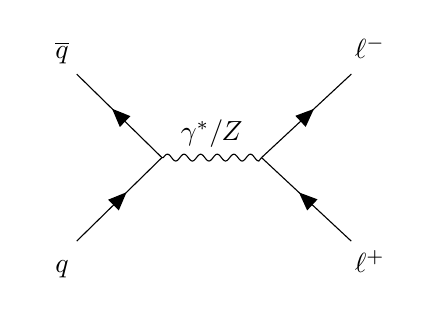
\begin{tikzpicture}\begin{feynman}[medium]
    \vertex (p1);
    \vertex [right=3.6em of p1] (p2);
    \vertex [above left=of p1] (qa){\(\phantom{^+}\qbar\)};
    \vertex [below left=of p1] (qb){\(\phantom{^+}q\)};
    \vertex [above right=of p2] (h){\(\ell^{-}\phantom{\qbar}\)};
    \vertex [below right=of p2] (v){\(\ell^{+}\phantom{\qbar}\)};
    \diagram* {
    (qb) --[fermion] (p1) --[fermion] (qa),
    (p1) --[boson,edge label=\(\gamma^*/Z\)] (p2),
    (v) --[fermion] (p2) --[fermion] (h),
    };
\end{feynman}
\end{tikzpicture}
}}
\subfloat[][]{{
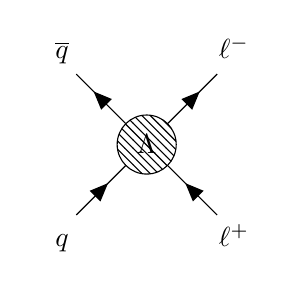
\begin{tikzpicture}\begin{feynman}[medium]
    \vertex [blob] (p1){\(\lam\)};
    \vertex [above left =4.80em of p1] (qa){\(\phantom{^+}\qbar\)};
    \vertex [below left =4.80em of p1] (qb){\(\phantom{^+}q\)};
    \vertex [above right=4.80em of p1] (h){\(\ell^{-}\phantom{\qbar}\)};
    \vertex [below right=4.80em of p1] (v){\(\ell^{+}\phantom{\qbar}\)};
    \diagram* {
    (qb) --[fermion] (p1) --[fermion] (qa),
    (v) --[fermion] (p1) --[fermion] (h),
    };
\end{feynman}
\end{tikzpicture}
}}
\caption{Feynman diagrams representing (a) Drell-Yan, which dominates the standard model contribution to high invariant-mass dilepton production, and (b) a contact interaction of energy scale \lam corresponding to one of the composite models described in Equation \ref{eqn:compLagrangian}.}
\label{fig:ciPheno}
\end{figure}


% \begin{figure}[h!]
% \captionsetup[subfigure]{position=b}
% \centering
% \subfloat[][]{{
% \feynmandiagram [medium,baseline=(v.base),horizontal=v to b] {
% i1 [particle=\(q\)] -- [fermion] v -- [fermion] i2 [particle=\(\qbar\)],
% v -- [photon, edge label=\(\gamma^*/Z\)] b,
% f1 [particle=\(\ell^{+}\)] -- [fermion] b -- [fermion] f2 [particle=\(\ell^{-}\)],
% };
% }}
% \subfloat[][]{{
% \feynmandiagram [medium,baseline=(v.base),horizontal=a to c] {
% a[particle=\(q\)] --[fermion] v[blob,label=\(\lam\)] --[fermion] b[particle=\(\qbar\)],
% c[particle=\(\ell^{+}\)] --[fermion] v --[fermion] d[particle=\(\ell^{-}\)],
% };
% }}
% \caption{Feynman diagrams representing (a) Drell-Yan, which dominates the standard model contribution to high invariant-mass dilepton production, and (b) a contact interaction of energy scale \lam corresponding to one of the composite models described in Equation \ref{eqn:compLagrangian}.}
% \label{fig:ciPheno}
% \end{figure}

Contact interactions necessarily modify cross-sections of fermion elastic scattering, such as the $q\qbar$ collisions at the LHC.
In the SM, the gauge coupling $\alpha_f$ controls high-mass processes through Drell-Yan production.
In their seminal work of 1983, Eichten, Lane, and Peskin showed that if $\alpha_f\llt1$, then the Lagrangian in Equation \ref{eqn:compLagrangian} produces interference of the order $\shat/\alpha_f\lam^2$ with the standard model processes \cite{eichten}.
The diagrams for the dominant standard model process and a generic contact interaction are shown in Figure \ref{fig:ciPheno}.
The blob in the diagram for the contact interaction emphasizes the generality of Equation \ref{eqn:compLagrangian}. A particular physics model may replace this blob with, for example, an s-channel diagram mediated by the bound state of two component prions.
Two possible diagrams to replace the blob are given, for illustrative purpose, in Figure \ref{fig:ciBlobs}.

Since these interactions depend on $q\qbar$ initial states, the relevant parton luminosities that determine the event rates are those of $u\ubar$ and $d\dbar$.
Unfortunately, as illustrated in Figure \ref{fig:partDistFunc}, proton PDFs for $\ubar$ and $\dbar$ are relatively small since these are produced as virtual sea quarks.
This suppresses the production of $q\qbar$ initial states, and consequently, of this type of contact interaction.
If the LHC had been designed to use $p\pbar$ collisions of equal intensity, it would greatly enhance the $q\qbar$ luminosities.

\begin{figure}[h!]
\captionsetup[subfigure]{position=b}
\centering
% \subfloat[][]{{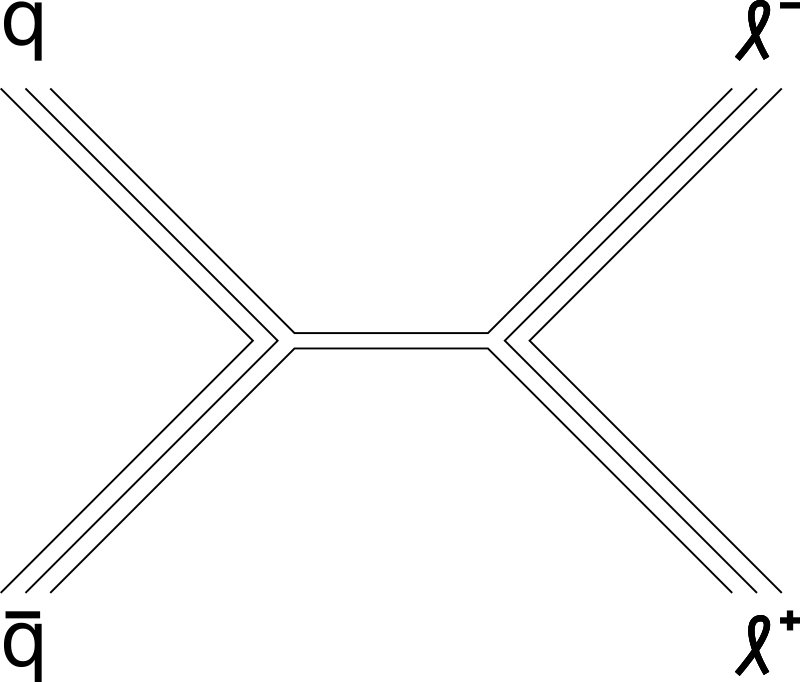
\includegraphics[height=0.20\textheight]{figures/pheno/ciSchan.png}}}
\subfloat[][]{{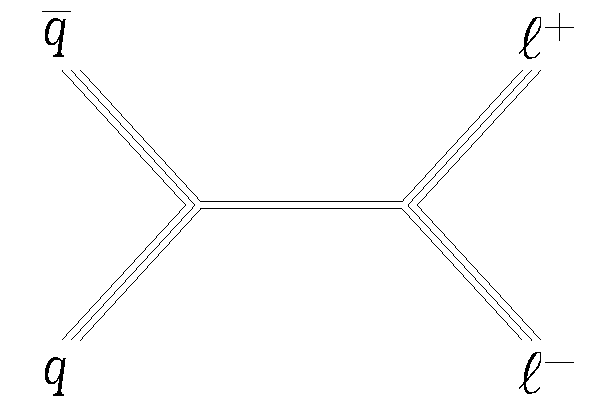
\includegraphics[height=0.20\textheight]{figures/pheno/ci-tchan.pdf}}}
\hspace{0.15\textwidth}%
% \subfloat[][]{{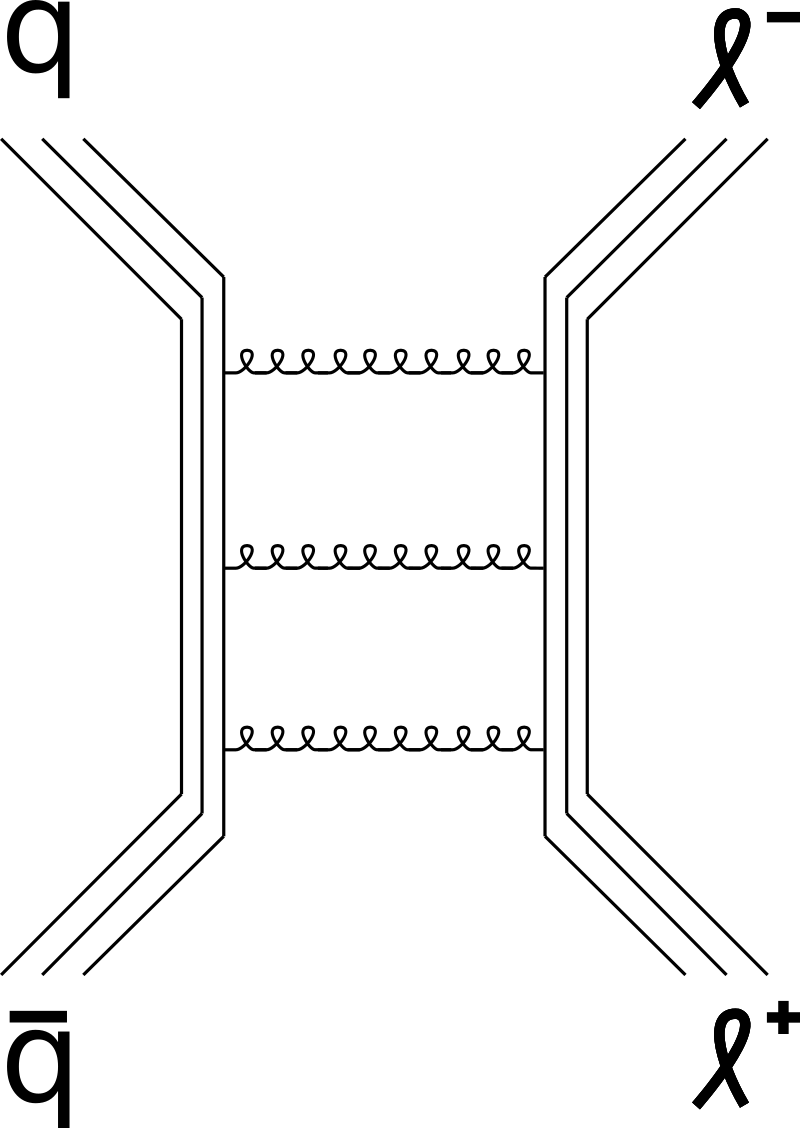
\includegraphics[height=0.20\textheight]{figures/pheno/ciGluon.png}}}
\subfloat[][]{{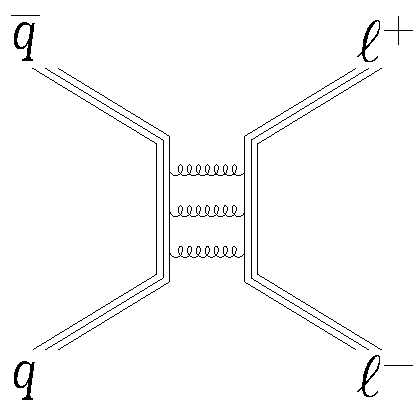
\includegraphics[height=0.20\textheight]{figures/pheno/ci-gluon.pdf}}}
\caption{Feynman diagrams for two possible high-energy processes that may result from fermion compositeness. The solid lines represent the preons composing the fermions. (a) An interaction mediated by the bound state of two prions, which is only possible when the leptons and quarks share common constituents. (b) An interaction between quarks and leptons mediated by \emph{metacolor gluon} exchange, represented by curly lines in analogy to SU(3) gluons.}
\label{fig:ciBlobs}
\end{figure}

%%% Specific ll-qq CI $$$
This thesis focuses on \llqq contact interactions, a subset of those described by Equation \ref{eqn:compLagrangian}.
Such models replace the unprimed $f$ with quarks, and the primed $f'$ with leptons.
This interaction is possible if the quarks and leptons share common constituents, in which case interactions mediated by the constituents are possible, as shown in Figure \ref{fig:ciBlobs} (a).
This interaction is also possible if the fermions do not share common constituents, as shown in Figure \ref{fig:ciBlobs} (b).

The Drell-Yan differential cross-section is modified in the case of left-left compositeness, $\eta_{LL}=\pm1$ and $\eta_{LR}=\eta_{RL}=\eta_{RR}=0$.

\begin{flalign}\label{eqn:}
\frac{d\hat{\sigma}}{d\that}(q_i\qbar_i\to\ll) =& \frac{\pi\alpha^2}{\shat^2}\left[A_i(\shat)\left(\frac{\uhat}{\shat}\right)^2+B_i(\shat)\left(\frac{\that}{\shat}\right)^2\right] \notag\\
\end{flalign} 
Here, the coefficients are defined as functions of \shat.
\begin{flalign}\label{eqn:}
A_i(\shat) =& \left[Q_i-\frac{L_iL_l}{4x_W(1-x_w)}\frac{\shat}{\shat-M_Z^2+iM_Z\Gamma_Z}-\frac{\eta_{LL}\shat}{\alpha\lam^2}\right]^2 + \notag\\
            & \left[Q_i-\frac{R_iR_l}{4x_W(1-x_w)}\frac{\shat}{\shat-M_Z^2+iM_Z\Gamma_Z}\right]^2  \notag\\
B_i(\shat) =& \left[Q_i-\frac{R_iL_l}{4x_W(1-x_w)}\frac{\shat}{\shat-M_Z^2+iM_Z\Gamma_Z}\right]^2 + \notag\\
            & \left[Q_i-\frac{L_iR_l}{4x_W(1-x_w)}\frac{\shat}{\shat-M_Z^2+iM_Z\Gamma_Z}\right]^2  \notag\\
\end{flalign}
In these equations, $i,j\in\{u,d\}$ stand for quark flavors.
As was defined when discussing Higgs production in Section \ref{sec:phenoHiggs}, $L_i=T_3-2Q_ix_W$, $R_i=-2Q_ix_W$, and $x_W=\sin^2\theta_W$. %{\color{red} coordinate notation}
$Q_i$ is the electric charge of the corresponding quark flavor \cite{Eichten:1984eu}. % supercollider

Despite their verbosity, these equations readily illuminate the phenomenology relevant to the contact interaction search.
First, when setting $\eta_{LL}=0$, the standard model Drell-Yan production is recovered.
Expanding the first power term in $A_i(\shat)$ yields a \emph{direct} term that contributes to the total cross-section and scales as $\lam^{-4}$.
Removing the \lam defines the contact interaction form factor $F_C$,
\begin{equation}\begin{split}
    % \Delta\left[\frac{d\hat{\sigma}}{d\that}\right] = \frac{\pi\alpha^2}{\shat^2}\left[\frac{\shat}{\alpha^2}\left(\frac{\uhat}{\shat}\right)^2 \right] /\lam^4
    F_C(\shat) \equiv \frac{\pi\uhat^2}{\shat^2}.
\end{split}\end{equation} 
Since $F_C$ is strictly positive, it enhances the total \qqll cross section regardless of the sign of $\eta_{LL}$.
The cross-terms in the expansion dictate the interference of the contact interaction with Drell-Yan.
Again removing the \lam factor defines the interference form factor $F_I$,
\begin{equation}\begin{split}
    F_I(\shat) \equiv -2\left[Q_i-\frac{L_iL_l}{4x_W(1-x_w)}\frac{\shat}{\shat-M_Z^2+iM_Z\Gamma_Z}\right]\frac{\pi\alpha\uhat^2}{\shat^3}.
\end{split}\end{equation} 
The sign of $F_I$ depends on the sign of $\eta_{LL}$.
For $\eta_{LL}=-1$, $F_I$ contributes constructively to the total cross-section, while for $\eta_{LL}=+1$ it leads to destructive interference that reduces the overall cross-section.

Together, $F_I$ and $F_C$ describe the effect of contact interactions as functions of collision energy, without referring to the particular manifestation of fermion compositeness.
The functional dependence on \shat leads to the expression of the interference form factor $F_I$ at relatively low energies than the direct form factor $F_C$.
Experimentally, this results in interference effects altering dilepton spectra at lower invariant-mass and direct production always enhancing the spectra in the high mass tail.
These effects are broad in the invariant-mass spectra instead of the narrow resonance expected from \hmm production.
The modification to the total cross section has the form,
\begin{equation}\label{eqn:cixsPheno}
\frac{\text{d}\sigma}{\text{d}m_{\ell\ell}} = \frac{\text{d}\sigma_\textrm{DY}}{\text{d}m_{\ell\ell}} - \eta_{ij}\frac{F_\textrm{I}}{\Lambda^2} + \frac{F_\textrm{C}}{\Lambda^4}.
\end{equation}

Although various compositeness models predict variations on these results, there are two points to consider.
First, the functional dependence on the energy \shat is common for all contact interactions \cite{Eichten:1984eu}.
Second, the modification to the effect on the total cross-section is of the same magnitude regardless of the form of compositeness.
Combined, these make the described formalism an attractive framework to study compositeness without reference to the particular model.


% \cite{acosta} % LHC prospect

\section{Physics Modeling with Simulation} \label{sec:phenoSim}

The dataset collected by the ATLAS experiment is both of limited size and of opaque nature.
It is limited because of the enormous effort required to run the LHC and operate the experiment.
It is opaque because many aspects of the collision are inaccessible to observation; from the initial state of the protons, to the intermediate physics processes, and to the kinematics of final state neutrinos, some observations are not technically feasible.
% As a result, the 
Even the collision's final state is imperfectly known due to the limited acceptance and detection efficiency of the experiment.
In light of these challenges, it is helpful to simulate collisions computationally and the resulting detector response to produce simulated datasets.

Simulated datasets are used for several purposes.
Because events are simulated based on particular Feynman diagrams, it is possible to explore how those diagrams contribute to the dataset.
% Use 1) composition
This is particularly helpful when considering kinematic distributions, such as the dilepton invariant-mass spectra.
In these, the simulation illuminates the composition of both signal and background distributions.
% Use 2) signal model
With this information, choices may be made to improve the sensitivity of the analysis to new physics signatures.
These include choices of the criteria that define the fiducial region of a search, or choices of the functional form that well describes the shapes of the background distributions.
In the \hmm analysis, simulated datasets are used to develop a multivariate discriminant tuned to identify signal-like events.
% Use 3) signal model
The simulated signal dataset is also useful to model the shape and amplitude of the signal when performing hypothesis tests.
This provides a map from a signal hypothesis's theoretical descriptions to experimentally testable predictions about event yields and distributions.
% Use 4) Systematics
Finally, simulated events provide a means to understand the performance and systematic uncertainties of the ATLAS detector itself.

Since they share many aspects, this section describes how simulated datasets are produced for both the \hmm and \nr analyses.
The procedure begins with event simulation, where a particular set of interactions are represented based on their matrix element.
This step is performed by an \emph{event generator} program.
The matrix element only describes the immediate interaction, or hard-scatter process, and the associated underlying event.
The event generation produces a particle description of the immediate aftermath of a collision. This is described in Section \ref{sec:evtGen}.
After this, strongly charged quarks and gluons undergo parton showering and hadronization.
The next step in the simulation describes these processes and results in a set of long-lived particles. This is described in Section \ref{sec:hadronization}.
The final step is the propagation of these particles through the magnetic field and detectors of the experiment.
This is performed with a simulation of the detector's materials described in Section \ref{sec:geant}.

\subsection{Event Generation} \label{sec:evtGen}

An event generator is a program that randomly samples several probability density functions (PDFs)\footnote{Care must be taken to avoid confusion of probability density functions with parton distribution functions. In the remaining text, the abbreviation PDF refers to the former.} in order to describe a set of possible collision events.
In its present usage, they are concerned with producing events corresponding to the hard-scattering processes corresponding to a set of Feynman diagrams, but not the long-term evolution of the final state particles.
The PDFs sampled include the parton distribution functions that describe the initial state of interactions.
They also include the normalized matrix elements under consideration, which describes the likelihood for particular final states to occur.
Through repeated sampling, the Monte-Carlo method, the set events begin to represent the events one might expect from a particular set of initial state conditions.

Different event generators are available with various strengths and weaknesses.
The work of this thesis uses samples produced primarily by \sherpa \cite{Gleisberg:2008ta} and \powheg \cite{Alioli:2010xd,Frixione:2007vw}.
In two instances, \pythia \cite{pythia8} and \madgraph \cite{Alwall:2014hca} are selected to produce signal events.

The parton distribution function also varies depending on the process being simulated.
Most simulated datasets are produced with NNPDF3.0NLO \cite{Ball:2014uwa}, and CT10 \cite{ct10}.
In some cases, variations such as NNPDF23LO \cite{Ball:2012cx} or NNLOPS \cite{Hamilton:2013fea} are used.
When unavoidable, PDF4LHC \cite{Butterworth:2015oua} is used.

% % hmm 
% Sherpa 2.2.1 with NNPDF3.0 DY
% Sherpa 2.2.2 with NNPDF3.0 diboson
% Powheg-Box v2 using NNPDF3.0 and Pythia 8.186 for parton showing and A14 param set ttbar
% Powheg-box v2 using NNLOPS (NNLO), PDF4LHC15, Pythia8 showerHadron ggH
% Powheg-box v2, Pythia8 shower/had NLO VBF and VH
% Powhegbox LO ggZH
% MG5_aMC@NLO with NNPDF3.0NLO and Pythia8 showerHadron

% % NR
% Powheg-Box and CT10, NLO: DY
% Powheg-Box and NNPDF3.0 NLO: top
% Sherpa 2.2.1 with CT10: Diboson
% Powheg-Box and NNPDF23LO, NLO: LO DY for Signal


\subsection{Showering and Hadronization} \label{sec:hadronization}

The hard-scattering process describes a final state, including strongly charged and unstable particles.
These can radiate photons, quarks, and gluons in a process called parton showering (PS).
In principle, the initial state partons may also radiate and contribute to PS in an event.
The PS calculation focuses on soft radiation, while the matrix element is used to describe hard radiation.
This division is necessary since the matrix element tends toward infinity as the radiation becomes increasingly soft.
A mixing scheme is used to blend these to produce an accurate description of PS.

Eventually, the final-state quarks and gluons separate and hadronize into color-neutral states.
Since this process is difficult to model from physical principles, it is based on a statistical sampling of the phase space available to the final state particles.
Programs make use of PDFs that have been adjusted to match experimental observation.

There are several programs capable of modeling PS and hadronization.
The event generator \pythia is also capable of modeling both and is used to process most simulated datasets.
The program \evtgen \cite{Lange:2001uf} complements \pythia by modeling bottom and charm hadron decays.
The event generator \sherpa is also used in some cases for PS.
The result of these steps is events of relatively stable ($c\tau>1$~cm) particles, including photons, leptons, and hadrons.
Before reconstruction, such an event is referred to as the \emph{truth} event and consists of \emph{truth particles}.
Truth events are useful in order to evaluate the performance of the detector, as well as the accuracy of the following analysis.


% % Hmm
% For MC using Pythia8-> EvtGen 1.2.0 used for bottom/charm decays

\subsection{Detector Simulation} \label{sec:geant}

\begin{figure}[h!]
\captionsetup[subfigure]{position=b}
\centering
\subfloat[][]{{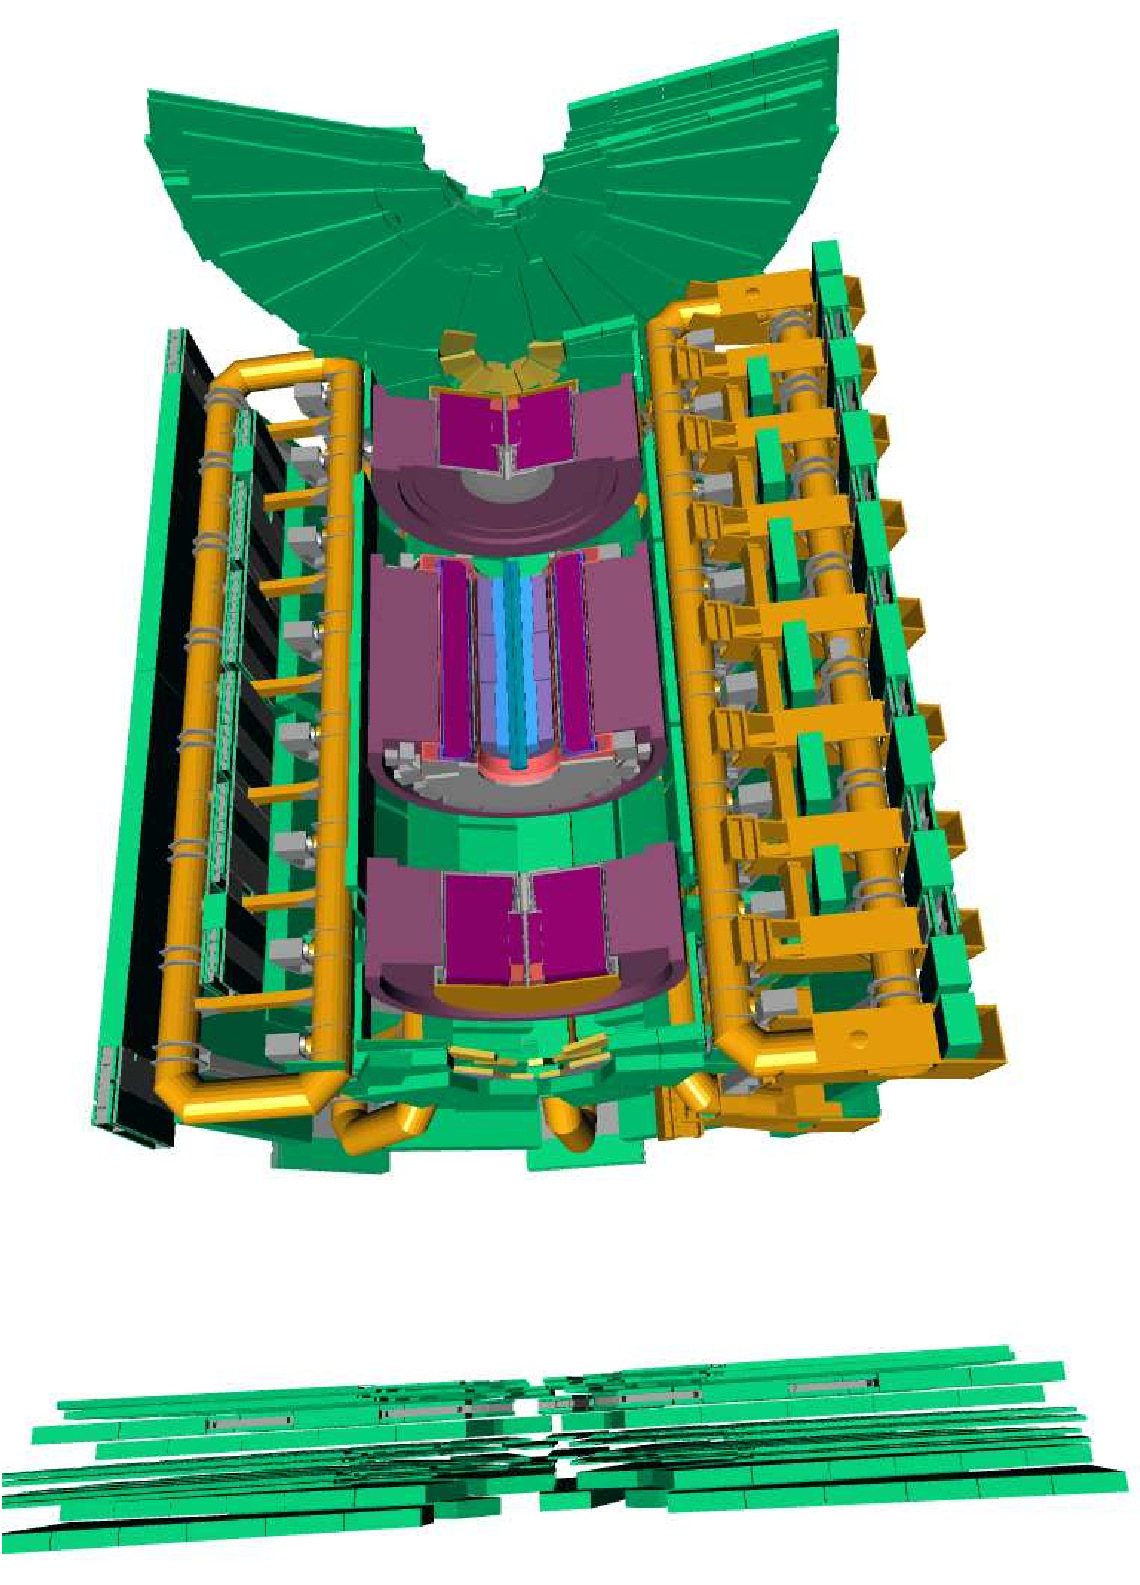
\includegraphics[angle=-90,width=0.7\textwidth]{figures/pheno/atlasSim.pdf}}}
\caption{Graphical representation of the  ATLAS detector in the \geant simulation, with a section of the barrel removed for visibility. The muon system is shown in green, the calorimeters are shown in purple, and the ID is shown in blue. Material that is not part of the detector systems, such as the support structures and magnets, are included in the simulation as well.}
\label{fig:atlasGeantSim}
\end{figure}

The final step is to simulate the response of ATLAS to the simulated events.
This is the closest approximation to the measured dataset.
It is also the most computationally intensive step, as it necessitates a full simulation over time of particle interactions within ATLAS.
The simulation is based on \geant \cite{geant}, and is part of the ATLAS simulation infrastructure \cite{SOFT-2010-01}.
The \geant model of ATLAS consists of nearly five million simulated volumes of both detectors and supporting structures in which particles may interact.
An illustration of the components of the simulation is shown in Figure \ref{fig:atlasGeantSim}.
A three-dimensional map of the magnetic field within ATLAS is included in the simulation as well.
The simulation transports truth particles through the magnetic field and detector volumes.
When a particle enters a detector volume, its interactions with the detector and the corresponding readout electronics are simulated.
The output of the readout electronics simulation is of the same format as the physical detector's output.
After this point, the simulated events can be routed through reconstruction identically to data.


% \input{sections/phenomenology-objects}

\chapter{Datasets and Objects}\label{sec:objectsDatasets}

The two studies described in this thesis are based on data recorded during Run~2 between 2015 and 2018.
This chapter lists the details of these datasets in Section \ref{sec:physData}, as well the simulated datasets used in Section \ref{sec:physSim}.  
Section \ref{sec:physObjects} describes the physical objects reconstructed from the events in these datasets.


\section{Recorded Dataset}\label{sec:physData}

Both searches use the full dataset collected by ATLAS during the Run~2 of the LHC.
Only events recorded during good operation of the detector are used.
The Good Run Lists (GRL) identify the data taking periods during which the data used for analysis was collected.
Table \ref{tab:GRLs} summarizes the datasets and luminosities for each year.

\begin{table}[H]
        \caption{Data luminosities for events delivered to ATLAS and for events passing the GRL requirement with the corresponding uncertainty, by year\cite{ATLAS-CONF-2019-021}.}
    \begin{center}\small
        \begin{tabular}{cr r rr}
            \toprule
            Year & Delivered & Recorded [\fb] & Uncertainty [\fb] \\
            \midrule
            2015-16 & 42.5 & 36.2 & 0.8 \\
            2017    & 50.2 & 44.3 & 1.0 \\
            2018    & 63.4 & 58.5 & 1.2 \\
            \midrule
            Total   & 156.1 & 139.0 & 2.4 \\
            \bottomrule
        \end{tabular}
        \label{tab:GRLs}
    \end{center}
\end{table}

The luminosity is measured using the ATLAS calorimeters and two dedicated Cherenkov radiation detectors, LUCID2, located 17~m from the interaction point in the A and C sided.
The collision luminosity is determined on a bunch-by-bunch basis using the signal strength from LUCID2 and the calorimeters.
The combined luminosity of the Run~2 collisions recorded and passing the GRL requirement is 139.0~fb$^{-1}$$\pm$1.7\% \cite{ATLAS-CONF-2019-021}.

\section{Simulated Datasets}\label{sec:physSim}

Simulated datasets serve a variety of roles in both analyses.
Both analyses deal with relatively weak mechanisms of signal production and relatively voluminous processes of background production.
If present, the signal processes contribute to the ensemble of events produced in collisions.
Simulation is used to quantitatively understand the effect of a signal process.
The result is a dataset of simulated events produced by a particular mechanism.
This is useful in modeling the distributions of kinematic variables in signal events in order to carefully select a phase-space in which to search for signal events.
Signal simulation is also useful to predict the expected multiplicity of signal events.
Simulation is also used to understand the background processes.
In the case of the \hmm search, background processes include all production mechanisms in the Standard Model except for those involved in Higgs boson production.
In the case of the \nr search, background processes are defined more broadly to include any mechanism except for the contact interactions that are the target of the search.
In each case, simulated background datasets provide insight into the particular production mechanisms expected to contribute to the observed dataset.
Empirical models are developed and tested on the background datasets.

The simulation relies on a number of input parameters that are known to varying degrees.
Different values of these parameters leads to different predictions in the simulation, which corresponds to uncertainty in the predictions derived from the simulated datasets.
The impact of these uncertainties differers between the \hmm and \nr searches, and is described in their respective chapters.

The simulations are produced by a series of programs, as described in Section \ref{sec:phenoSim}.
The first program is a matrix element Generator, which uses the input of a particular parton density function (PDF).
Different event generators are available with various strengths and weaknesses.
The work of this thesis uses samples produced primarily by \sherpa \cite{Gleisberg:2008ta} and \powheg \cite{Alioli:2010xd,Frixione:2007vw}.
In two instances, \pythia \cite{pythia8} and \madgraph \cite{Alwall:2014hca} are selected to produce signal events.
The parton distribution function also varies depending on the process being simulated.
Most simulated datasets are produced with NNPDF3.0NLO \cite{Ball:2014uwa}, and CT10 \cite{ct10}.
In some cases, variations such as NNPDF23LO \cite{Ball:2012cx} or NNLOPS \cite{Hamilton:2013fea} are used.
When unavoidable, PDF4LHC \cite{Butterworth:2015oua} is used.
Next are programs that calculate the parton shower and hadronization.
In nearly all cases, \pythia and \evtgen are used to compute these effects.

The simulations are classed based on the precision to which the matrix element (ME) is calculated.
The exact evaluation of the ME corresponds to the evaluation of an infinite perturbative expansion of the Hamiltonian that governs the transition of the initial state to the final state.
This expansion can be made in terms of the coupling strengths of the interactions involved.
The degree of precision of the simulation corresponds to the number of terms, equivalently Feynman diagrams, included in the perturbative expansion.
This begins with the leading order (LO) calculation, which includes the set of Feynman diagrams with no closed loops.
Higher order calculations are performed beginning with next-to-leading order (NLO) which includes one-loop diagrams, and next-to-next-to-leading order (NNLO) with two loops.
The choice of precision depends on both the relative cross-section of the mechanism and how the simulation is to be used.
Mechanisms with a large cross-section are simulated with to high order to achieve a level of precision in the final prediction of the dataset.
Mechanisms with a low cross-section can be simulated to lower order and retain a similar level of precision.

The list of simulated datasets used in this work is provided in Table \ref{tab:simulatedDatasets}.


\begin{table}[htp]
\caption{Samples in the top are used in the \nr analysis, while samples in the bottom are used for the \hmm search. The dilepton production via Drell-Yan processes (\ee and \mm) are calculated to NLO precision with additional LO contributions from diagrams with three or four final state jets.}
\begin{center}
\resizebox{\textwidth}{!}{
\begin{tabular}{l l l l l l l l}
\toprule
    & Process           & QCD      & EW       & ME Generator           & PS and Hadronization \\
\midrule
\multirow{5}{*}[-1.5em]{\begin{sideways}\nr\end{sideways}}    
    & Drell-Yan         & NNLO     & NLO      & \powheg, CT10          & \pythia+\evtgen \\ % CTEQ6L1   
    & Drell-Yan         & LO       &          & \powheg, NDPDF23LO     & \pythia+\evtgen \\ % NNPDF23LO 
    & $t\overline{t}$   & NLO      &          & \powheg, NDPDF3.0NLO   & \pythia+\evtgen \\ % NNPDF23LO 
    & Single top        & NLO      &          & \powheg, NDPDF3.0NLO   & \pythia+\evtgen \\ % NNPDF23LO 
    & Diboson           & NLO      &          & \sherpa, CT10          & \sherpa \\ % CT10              
\midrule
\multirow{10}{*}[-1.5em]{\begin{sideways}\hmm\end{sideways}}    
    & Drell-Yan         & NLO      & NLO      & \sherpa, NNPDF30NNLO   &                            \\
    & $t\overline{t}$   & NNLO     &          & \powheg, NNPDF3.0LO    & \pythia+\evtgen            \\
    & Single top        & NNLO     &          & \powheg, NNPDF3.0LO    & \pythia+\evtgen            \\
    & Diboson           & NLO      &          & \sherpa, NNPDF3.0LO    & \pythia+\evtgen            \\
    & ggH               & NNLO     &          & \powheg, PDF4LHC15     & \pythia+\evtgen            \\
    & VBF               & NLO      &          & \powheg, NNPDF3.0      & \pythia+\evtgen            \\
    & $qq/qg\to WH$     & NLO      &          & \powheg, NNPDF3.0      & \pythia+\evtgen            \\
    & $qq/qg\to ZH$     & NLO      &          & \powheg, NNPDF3.0      & \pythia+\evtgen            \\
    & $gg   \to ZH$     & LO       & LO       & \powheg, NNPDF3.0      & \pythia+\evtgen            \\
    & ttH               & NLO      & NLO      & \madgraph, NNPDF3.0LO  & \pythia+\evtgen            \\
\bottomrule
\end{tabular}
}
\label{tab:simulatedDatasets}
\end{center}
\end{table}

% Normalization
Kinematic variables are calculated from the reconstructed final states in simulated events.
These variables form probability density distributions that reflect the likelihood of measuring a particular kinematic variable in an event from a given production mechanism.
Statistical fluctuations become less important as the number of the simulated events increases which makes the distributions more informative.
In general the event multiplicity in the simulated datasets exceeds that of the observed data by an order of magnitude.
To represent the observation, the simulated distributions are normalized to match a theoretically predicted cross section.
For ggF Higgs production simulation this normalization is based on three-loop (N3LO) QCD calculations and NLO EW calculations.
For other Higgs signals the QCD precision reduced to NNLO \cite{higgsCross}.
The cross section of Drell-Yan is calculated to NNLO precision.
The cross section of diboson processes is calculated to NLO precision.
The \ttbar cross section is available at NNLO precision, while the smaller single-top cross sections are calculated to NLO precision.
For the purpose of the \nr analysis, after the samples have been normalized to their predicted cross section, a common factor scales all the simulations to match the multiplicity of observed data in a control region. 


\section{Physics Object Reconstruction}\label{sec:physObjects}
The analyses presented in this thesis view the data collected by the ATLAS experiment through the abstraction of \emph{physics objects}.
It is worth noting that physics objects are not exactly isomorphic to the actual physical entities emanating from the collision.
These are patterns of detector hits and energy deposits that are construed to have some physical meaning.
In some cases, these patterns are clearly identified with particles like muons or electrons passing through the detector.
In other cases, the identification is more pragmatic for the purpose of analysis, as is the case when describing \emph{missing transverse momentum} ($E_T^\text{miss}$) as an object.
Somewhere in between these are clusters of energy deposits called \emph{jets}, which are identified as the result of the hadronization of quarks and gluons.

The difference between the ``physics object'' of a jet and the quark or gluon it is presumed to describe is clear.
Different definitions of ``cluster'' lead to different jet energies, and even different numbers of jets.
This subtlety in definition also applies to muons, electrons, and of course, $E_T^\text{miss}$.
The following section describes the choices made in defining the physics objects used in this thesis.

There are three steps in choosing what physics objects to use.
The first step is in the reconstruction algorithm, which arranges the data recorded in an event into reasonable approximations of particles and jets.
Next, some of these candidates are accepted or rejected based on identification criteria.
Finally, a secondary requirement of isolation is imposed on the objects to isolate objects originating directly, or promptly, from the collision.
This final step is particularly important in the context of this thesis, where prompt leptons are of primary interest.

\subsection{Electrons}
Electrons are reconstructed from data collected by the inner detector and electromagnetic calorimeter.
An electron passing through the ID typically produces four hits in the pixel layers and eight hits in the Silicon Tracker (SCT) layers, from which the track and impact parameter are established.
After passing through the silicon detectors, the electron produces transition radiation surrounding the Transition Radiation Tracker (TRT).
This helps identify electrons as relativistic charged particles.
Next, the electron enters the electromagnetic calorimeter, where it deposits most of its energy.
The segmented structure of the calorimeter measures both the energy deposited directly by the electron and subsequent showers of secondary particles.

The search for electron candidates begins with a scan of energy deposits in the calorimeter, searching for localized clusters in $\eta-\phi$ space.
Next, the hits in the inner detector pixel and SCT layers are grouped first by layer and then between layers to form tracks.
Calorimeter clusters with azimuth $\phi_\text{calo}$ and ID tracks with azimuth $\phi_\text{track}$ are matched with a fitting procedure.
A restriction $-0.10<\Delta\phi<0.05$ where $\Delta\phi=-q\times(\phi_\text{calo}-\phi_\text{track})$ and $q$ is the charge of the track is made, and the asymmetric range accounts for bremsstrahlung effects \cite{elecReco}.

\subsubsection{Identification}

The choice of which electron candidates to consider for analysis is made using a likelihood (LH) identification.
This quantifies the probability for a candidate electron to have been produced by a physical electron passing through the detector.
The goal is to identify prompt electrons (signal) from jets, photon conversion electrons, and hadronic decay electrons (background).
Fourteen quantities, $\vec{x}$, are measured for the candidate electron.
These quantities describe the distribution of energy in the calorimeter layers, the impact parameter from the ID, the momentum lost by the track over time, the TRT response, and the $\eta-\phi$ match between the track and calorimeter cluster.
The PDFs for their values, $\vec{P}_{S(B)}$, are measured from simulation for signal and background.


The likelihood for a candidate to be signal (background) is given in Equation \ref{eqn:elecLH}.
\begin{equation}\begin{split}\label{eqn:elecLH}
L_{S(B)}(\vec{x}) = \prod_{i=1}^{14}P_{S(B),i}(x_i)
\end{split}\end{equation}
The discriminant $d_L$ is defined in Equation \ref{eqn:discLH} and peaks near one for signal, and zero for background.
\begin{equation}\begin{split}\label{eqn:discLH}
d_L=\frac{L_S}{L_S+L_B}
\end{split}\end{equation} 
Electron candidates passing increasingly restrictive thresholds of $d_L$ comprise the \code{VeryLoose}, \code{Loose(AndBLayer)}, \code{Medium}, and \code{Tight} LH identification working points.
In this thesis, the \code{LooseAndBLayer} and \code{Medium} LH identifications are used.
Both additionally require at least two pixel hits and seven total hits in the silicon ID.
At least one pixel hit is required in the innermost working pixel layer.
These have efficiencies of 88\% and 80\% for electrons with \et=40~GeV, respectively.

Electrons that are reconstructed with a path traveling directly through a broken calorimeter cell are marked with the label \emph{BADCLUSELECTRON}.
It is helpful to exclude such electrons from consideration due to their poor \et measurement.

% NR:  LooseAndBLayerLLH (QCD Fakes), MediumLLH
% hmm: Medium LH
\subsubsection{Isolation}
The signal models of interest for this thesis lead to electrons produced in isolation from other particles.
These electrons originate promptly from the interaction point.
In order to identify such electrons, the activity within a $\eta-\phi$ cone of $\Delta R=\sqrt{(\Delta\eta)^2+(\Delta\phi)^2}$ is quantitatively by measures of charged tracks and calorimeter energy deposits.
A variable cone size of $\Delta R=\text{min}(0.2,10\text{GeV}/\pt)$ is used to count tracks with $\pt>1$~GeV around the electron. The \pt of the tracks within this cone, excluding the electron's tracks, are summed to define \ptvarconeElec.
The electron's ``tracks'' is plural to account for bremsstrahlung radiation converting to secondary electrons. 
These are counted as part of the electron candidate if the extrapolated track falls within $\Delta\eta+\Delta\phi=0.05\times0.1$ of the primary calorimeter cluster.
Meanwhile, a fixed cone size of $\Delta R=0.2$ is used to sum up the activity in the calorimeters.
First, the energy from the electron is subtracted within an area of $\Delta\eta+\Delta\phi=0.125\times0.175$.
Energy from pileup effects is subtracted, and the remaining \et is summed to define \etcone.

Two isolation schemes are used in this thesis.
The first, \code{FixedCutLoose}, enforces a requirement that $\etcone/\et<0.20$ and $\ptvarconeElec/\pt<0.15$.
The efficiency, $\epsilon_\text{iso}$, of this requirement for prompt electrons is $\approx99\%$.
These cuts perform well in the relatively narrow kinematic region of interest for \hmm, but the search for high-mass phenomena needs a more flexible scheme.
A dynamic isolation, \code{Gradient}, is defined as a function of the electron \et.
It is defined such that the efficiency $\epsilon_\text{iso}=0.1143\times\et+92.14\%$ is constant across $\eta$.
\cite{elecReco}


% NR:  gradient
% hmm: FCLoose

\subsection{Muons}

Data from both the inner detector and muon spectrometer can be used to reconstruct muons.
In the former case, a similar procedure to that used to reconstruct ID electrons is used.
In the latter case, an algorithm searches data from MS chambers for hits that follow plausible muon paths, called segments.
Then, starting from segments, candidate tracks are built by combinatorially including hits from tracks in other layers.
The best tracks are selected based on the $\chi^2$ fit quality and number of hits used.
Each track must contain at least two segments.
\footnote{There is an exception in the transition region between the barrel and endcap where one segment is sufficient, however such muons are excluded from consideration in this thesis.}

\subsubsection{Identification}

Four types of muons are reconstructed.
Combined muons (CB), which are reconstructed using tracks in the ID and MS.
\begin{itemize}
\item Segment-tagged muons (ST), which are built from ID tracks extrapolated to match MS hits.
\item Calorimeter-tagged muons, which are built using ID tracks extrapolated to match calorimeter energy deposits.
\item Extrapolated muons (ME), which are reconstructed using only the MS and the location of the interaction point.
\end{itemize}

Five criteria define the commonly used identifications: \code{Loose}, \code{Medium}, \code{Tight}, \code{Low}-\pt, \code{High}-\pt.
These working points admit or reject muons based on several variables:
\begin{itemize}
    \item The absolute difference between the charge to momentum ratio measured in the MS versus the ID, as a fraction of the sum in quadrature of the corresponding MS and ID uncertainties. This is the q/p significance.
    \item The absolute difference between the \pt measured in the MS vs the ID, as a fraction of the combined \pt. This is the $p'$ variable.
    \item The normalized $\chi^2$ of the combined track fit.
\end{itemize}
% Medium muons
The baseline identification for ATLAS searches is Medium, which begins with CB and ME muons.
CB muons are required to use at least three hits in two MDT layers, or one MDT layer and no more than one missing layer within $|\eta|<0.1$.
The later allowance is made due to lost coverage in the barrel.
ME muons are required to use at least three MDT/CSC layers and fall within $2.5<|\eta|<2.7$, where the ID loses coverage.
For all muons, the q/p significance must be less than seven.
\cite{muonReco}

% Loose muons
The choice of identification depends on the requirements of the analysis.
The searches in this thesis are performed using both expanded and restricted muon identifications.
The \hmm search is concerned with small yields of low-\pt muons; therefore, the \code{Loose} working point is used to maximize reconstruction efficiency.
The \code{Loose} identification is a superset of the \code{Medium} identification.
Additional CT and ST muons are allowed in $|\eta|<0.1$. This adds approximately 2.5\% more muons in the barrel region.
\cite{muonReco}

% High-pt muons
In contrast, the high-mass non-resonant search is concerned with more energetic muons.
For these, a subset of the Medium identification, the \code{High}-\pt identification, is used to reduce incorrectly reconstructed muons.
CB muons otherwise passing the Medium criteria must have three hits in three MS stations.
Some regions of the MS are excluded based on their alignment accuracy.
This restriction trades efficiency to improve \pt resolution by approximately 30\% for muons with $\pt>1.5$ TeV.
It reduces the reconstruction efficiency by $\approx$20\% but improves \pt resolution above 1.5 TeV by $\approx$30\%.
\cite{muonReco}

\subsubsection{Isolation}

As is the case for electrons, the muons of interest in this thesis originate promptly from the interaction point, either from the decay of a Higgs boson or through a contact interaction.
Both types of processes are expected to produce muons that are isolated from other particles in the event.
In contract, semi-leptonic decays and hadronic decays produce muons in close proximity to other particles.
To identify the muons of interest, the concept of isolation is quantified by the sum of tracks in a variable size cone around the muon.
Four related variables are defined.
First variable is \ptvarconeMuon, which is defined as the scalar sum of \pt for tracks within a cone size $\Delta R=\text{min}(0.3,10\text{GeV}/\pt)$. Only tracks with $\pt>1$~GeV are counted, and the muon \pt is excluded.
The second and third variables are \etcone and \ptcone, which are defined as the scalar sum of \et or \pt, respectively, within a cone size of $\Delta R=0.2$.
The fourth variable, \neutralcone, is similar to \etcone. It is the sum of neutral \et within a cone size of $\Delta R=0.2$.

These variables are used to define the three isolation working points used in this thesis.
The first, FixedCutTightTrackOnly, simply required $\ptvarconeMuon/\pt<0.06$.
The second is FixedCutPflowLoose, which requires both $\ptvarconeMuon+0.4\neutralcone)/\pt<0.16$ and $\ptcone+0.4\neutralcone)/\pt<0.16$.
The third is FixedCutLoose, which requires both $\ptvarconeMuon/\pt<0.15$ and $\etcone/\pt<0.30$.
While the efficiency of these isolation requirements varies with \pt, in general, fewer than 1\% of prompt muons are lost.
\cite{muonReco}

\subsubsection{Bad Muon Veto}\label{sec:bmv}

In the high-\pt regime, it becomes difficult to accurately reconstruct muons due to the small bending radius in the magnetic field.
A criteria named \emph{Bad Muon Veto} (BMV) is used to address this by ignoring poorly reconstructed muons in the tails of the relative \pt resolution distributions, $\sigma_{\pt}/\pt$, given in Equation \ref{eqn:muonRes}.

\begin{equation}\begin{split}\label{eqn:muonRes}
    \frac{\sigma(p)}{p}=(\frac{p_0}{\pt}\oplus p_1 \oplus p_2\times \pt)
\end{split}\end{equation} 
The parameters $p_0$, $p_1$, and $p_2$ are measured for the MS and ID in different $\eta$ regions. 
The first term describes uncertainty in energy loss as a muon travels through detector material and becomes less impactful at higher \pt.
The second term covers multiple scattering and irregularities in the magnetic field.
The third term dominates at high-\pt and describes the intrinsic spacial resolution of the muon detectors, including the accuracy of their alignment \cite{muonReco}.
A cut is made on the relative uncertainty:
\begin{equation}
\frac{\sigma(q/p)}{(q/p)} < C(\pt)\cdot \sigma_{rel}^{exp}.
\end{equation}
Here $C(\pt)$ is a \pt-dependent coefficient which is equal to 2.5 when $\pt<1$~TeV and decreases linearly above this.
The application of the BMV reduces efficiency by 7\% for high-\pt muons, while removing poorly reconstructed muons that should not be considered for analysis.

% Isolation
% NR: FCTightTrackOnly
% hmm: FixedCutPflowLoose

\subsection{Jets}\label{sec:expJets}

Strongly charged quarks and gluons exiting a collision hadronize, producing to a collimated jet of heavier particles.
Since none of the final states under consideration in this thesis include quarks or gluons, it is helpful to exclude their presence in some cases.
To this end, jets are reconstructed such that events that contain them may be excluded.
Charged tracks from the ID are associated to calorimeter regions to remove associated deposits using the PFlow algorithm \cite{jetReco}.
The remaining energy is grouped using together by considering pseudo-distance measure between two energy deposits $i$ and $j$,
\begin{equation}\begin{split}
d_{ij} =& \text{min}(p^{-2}_{\text{T}i},p^{-2}_{\text{T}j})\frac{\Delta_{ij}^2}{R^2},
\end{split}\end{equation} 
where $k_{\text{T}i}$ and $p_{\text{T}j}$ are the cluster energies, $\Delta_{ij}=\sqrt{(\Delta y)^2+(\Delta\phi)^2}$ is their separation in rapidity and azimuth, and $R$ is a parameter set to 0.4.
The proceeds by finding the minimum of the set $\{d_{ij},p^{-2}_{\text{T}i}\}$ for all clusters $i$ and $j$. 
If $d_{ij}$ is the minimum, clusters $i$ and $j$ are combined into one.
If $p^{-2}_{\text{T}i}$ is the minimum, then cluster $i$ is considered to be a jet and is removed from the set.
Minima are found and removed until none remain.
This defines all the jets in the event \cite{antikt}.

Jets originating from bottom quarks and the decay of B-hadrons (b-jets) are of particular interest for the \hmm analysis.
A multivariate discriminant, MV2c10, is helps to distinguish b-jets from other light jets \cite{btag}.
This separates the b-jets from light flavor jets based on the characteristic displaced vertices of their associated tracks.
An identification that tags 85\% of b-jets defines the ``b-tag working point'' that proves useful to reject events, including b-jets.

\subsection{Missing transverse momentum}

The final ``object'' to consider in events is the missing transverse momentum, \met.
The transverse momenta of muons, electrons, and the remaining tracks in the ID are summed to produce the total measured \pt of the event.
Since the total \pt of the initial state is close to zero, the negative of this \pt sum represents the \pt of objects that have not been reconstructed \cite{met}.
The \met of an event is a helpful proxy for high-\pt neutrino, which carry \pt without detection.
This makes \met useful in the \hmm search when identifying the decay of \W to leptons and neutrinos.
In events with high-\pt muons, mis-measured muon \pt also appears in the \met sum.
This makes \met useful in the search for high-mass phenomena to study such muons.



% % % % \chapter{Statistics}

\section{Definitions}
\subsection{Likelihood}
\subsection{CLs}
\subsection{Significance}
\subsection{Limits}

\section{Approaches to Statistics}
\subsection{Frequentist Methods}
\subsection{Bayesian Methods}
\subsection{Hybrid Methods}

% results
\section{Analyzing Data}
\subsection{Fitting Procedures}
\subsection{Measuring Significance}
\subsection{Setting Limits}

\chapter{Higgs Decays to Two Muons}\label{sec:hmumu}


The joint observation of the Higgs boson by ATLAS \cite{atlashiggs} and CMS \cite{cmshiggs} in 2012 initiated an era of studies of this particle and its interactions.
One of the reasons that the Higgs boson is interesting is that the Englert-Brout-Higgs (BEH) mechanism generates the mass of fermions by means of Yukawa couplings to the Higgs boson.
The most direct way to study these couplings is through the fermionic decay of the Higgs, described in Section \ref{sec:phenoHiggs}.
As the fermion branching ratios given Equation \ref{eqn:higgsDecayFermions} indicate, the Yukawa coupling is proportional to the fermion mass squared.
The $H\to\ttbar$ decay is kinematically forbidden because the top quark mass, $m_t\approx173$~GeV, exceeds the mass of the Higgs boson.
Consequently, the most probable decay path is to bottom quark pairs due to their large mass $m_b=4.2$~GeV. 
Despite this, the $H\ttbar$ coupling can be measured through the ttH process described in Table \ref{tab:higgsProdDiagrams}.
The $Hb\bbar$ coupling was observed at the ATLAS experiment using the VH production channels \cite{atlasHbb}.
The next most massive fermion after the bottom quark is the tau lepton, with $m_\tau=1.8$~GeV, which has been studied by ATLAS \cite{atlasTauTau} and CMS \cite{cmsTauTau}.
% I don't want the thesis to be immediately out of date
Although the charm quark with follows with a mass $m_c=1.3$~GeV, the messy hadronization of final state proves difficult to identify and study.
Searches for $H\to c\cbar$ remain insensitive even to $Hc\cbar$ couplings $\sim100$ times the Standard Model expectation.
This leaves the muon and the $H\mm$ coupling, where the muon's mass of $\m_\mu=0.1$~GeV results in a challengingly small branching fraction.
However, unlike the case with the charm quarks, the final state of two muons is easily identified by a clear experimental signature.
The result is that the $H\mm$ is the third and most challenging Higgs Yukawa coupling that is feasible to study at ATLAS.

\begin{figure}[h!]
\captionsetup[subfigure]{position=b}
\centering
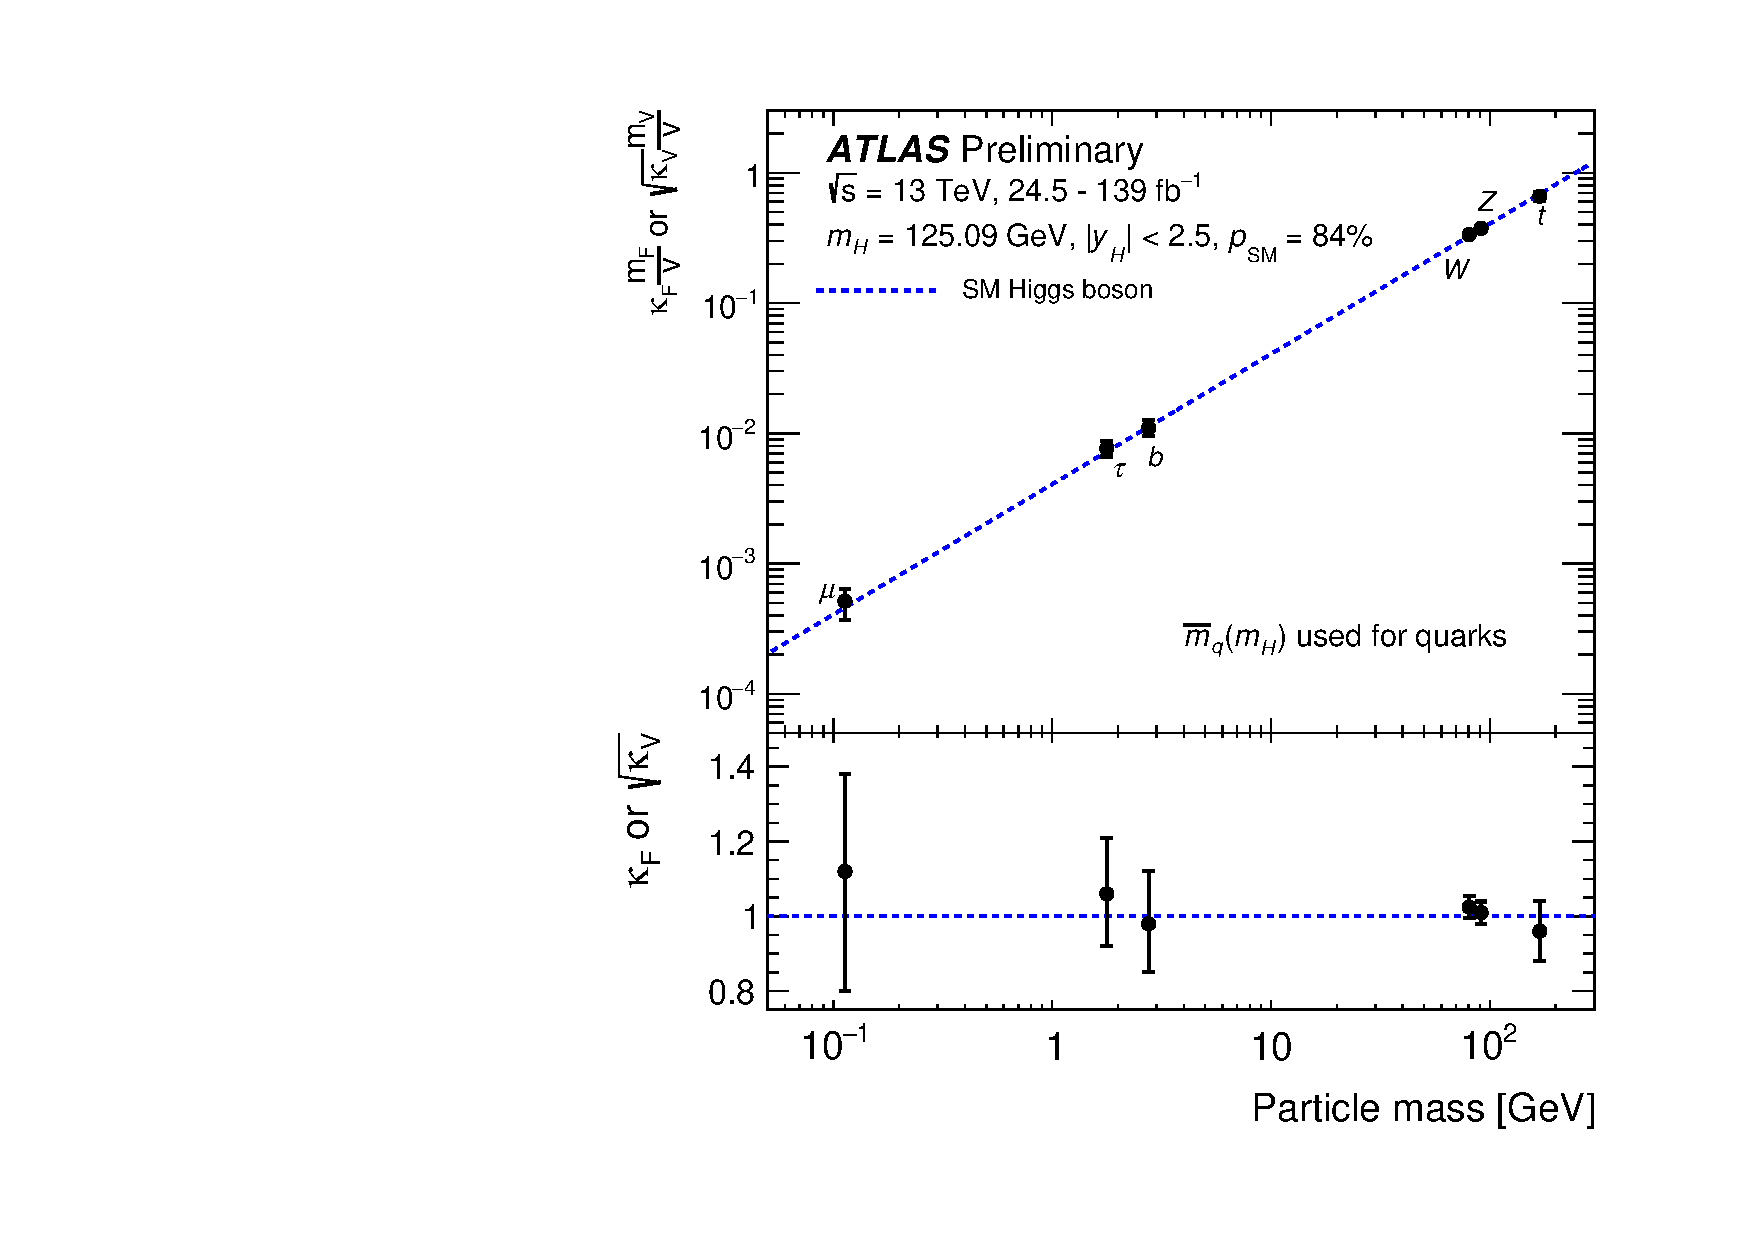
\includegraphics[width=0.7\textwidth]{figures/hmumu/massCouplingPlot.pdf}
\caption{Summary of ATLAS measurements of various fermion ($t$, $b$, $\tau$, and $\mu$) and gauge bosons. The plot shows the ``reduced coupling strength moderators'', where $\kappa$ is the deviation relative to the Standard Model prediction, compared to the particle's mass.
The SM prediction for both cases is also shown as a dotted line.
The contribution of this study appears in the bottom left corner of this plot. 
}
\label{fig:higgsMassCoupling}
\end{figure}

The $H\mm$ coupling also provides a unique opportunity as both the $Hb\bbar$ and $H\tautau$ couplings are to third-generation fermions.
This means that the \hmm measurement adds a valuable point to the global picture of Higgs couplings, as illustrated in Figure \ref{fig:higgsMassCoupling}.
Measuring this coupling provides a test of the Standard Model and also insight into the nature of the muon's mass.

Detecting the decays of Higgs to two muons is particularly challenging on two counts.
First, the Higgs branching fraction to muons is tiny ($2.18\times10^{-4}$).
Second, there is a sizeable irreducible dimuon background from Drell-Yan and Diboson processes.
Together these evoke the idiomatic needle-in-a-haystack to describe the search for \hmm.
It is only with the enormous number of events collected by ATLAS during the Run 2 data-taking campaign that it became feasible to perform this search.

%%%%%%%%%%%%% VH #################3

Of particular interest in this thesis are Higgs bosons produced through the VH production mechanisms.
These mechanisms are listed in Table \ref{tab:higgsProdDiagrams} as Higgs-strahlung and gluon-originated ZH.
They result in final states with a Higgs boson as well as an associated \W or \Z vector boson.
These events offer both a chance to look at a new, unstudied phase space, as well as a contribution to the overall sensitivity in the search for \hmm.
The events where the vector boson decays leptonically are particularly useful.
The additional leptons help differentiate VH events from the Drell-Yan background and provide kinematic information for further discrimination.

The cross-section of WH is 1.36~pb in center-of-mass collisions with energy $\sqrt{s}=13$~TeV, while the ZH cross-section is just 0.88~pb.

\begin{table}[htbp]
 \caption{Expected numbers of events from 139 fb$^{-1}$ $\sqrt{S}=13$ TeV data for WH and ZH. The first column shows the number of VH events, while the second column scales this by BR($H\to\mu\mu$) and the third column additionally multiplies by BR($V\to\ell\ell$) where $\ell$ is $e$ or $\mu$.}
 \begin{center}
\begin{tabular}{l c c c c}\toprule
% Production   & $H\to\mu\mu$ & $H\to\mu\mu,~V\to\ell\ell$ \\
Vector Boson  & VH & VH(\hmm) & VH(\hmm,~$^{W\to\ell\nu}_{Z\to\ll}$) \\
\midrule
V=\W & 189,040 & 41.5 & 9.14 \\
V=\Z & 122,320 & 26.9 & 1.83 \\
\bottomrule\end{tabular}
 \end{center}
\label{tab:vh-predict}
\end{table}

Studying \hmm with VH produced events introduces several challenges and opportunities.
First the tiny VH cross-section produces relatively few events to study.
Second is the question of how to use the new information from the leptonic vector boson decay products to separate the background from diboson production processes.
This information is particularly important to remove diboson (ZZ and WZ) backgrounds.
% Techniques to address challenge
Careful choices are made in the selection criteria targeted at VH production in order to capture as many VH/\hmm events as possible.
A multivariate analysis (MVA) discriminant is used to take advantage of the kinematic information in the \W and \Z decays.
Steps must be taken to understand and to limit the level of bias that these techniques introduce to the results. 
This is necessary to avoid invalidating the final measurements. 

\begin{figure}[htpb]
  \centering
    % \centered{\begin{tikzpicture}
    % \begin{feynman}
    %     \vertex (qa){\(\qbar\)};
    %     \vertex [below right=of qa] (p1);
    %     \vertex [below left=of p1] (qb){\(q'/q\)};
    %     \vertex [right=of p1] (p2);
    %     \vertex [above right=of p2] (h){\(H\)};
    %     \vertex [below right=of p2] (v){\(W/Z\)};
    %     \diagram* {
    %     (qb) --[fermion] (p1) --[fermion] (qa),
    %     (p1) --[boson,edge label=\(W/Z\)] (p2),
    %     (v) --[boson] (p2) --[scalar] (h),
    %     };
    % \end{feynman}
    % \end{tikzpicture}} 

\centered{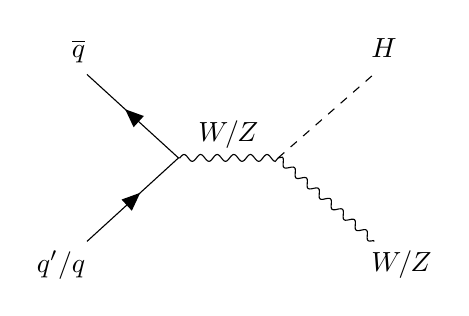
\begin{tikzpicture}\begin{feynman}[medium]
    \vertex (p1);
    \vertex [right=3.6em of p1] (p2);
    \vertex [above left=of p1] (qa){\(\phantom{q'/}\qbar\)};
    \vertex [below left=of p1] (qb){\(q'/q\)};
    \vertex [above right=of p2] (h){\(H\phantom{/Z}\)};
    \vertex [below right=of p2] (v){\(W/Z\)};
    \diagram* {
    (qb) --[fermion] (p1) --[fermion] (qa),
    (p1) --[boson,edge label=\(W/Z\)] (p2),
    (v) --[boson] (p2) --[scalar] (h),
    };
\end{feynman}
\end{tikzpicture}} 
  \caption{VH production originating from quarks}
    \label{fig:vh-prod}
\end{figure}

The VH production mechanisms, WH and ZH, exemplified in Figure \ref{fig:vh-prod}, are the third and fourth leading Higgs boson production mechanisms at the LHC.
The cross-section of WH is 1.36~pb in center-of-mass collisions with energy $\sqrt{S}=13$, while the ZH cross-section is just 0.88~pb.
The cross-section, combined with the branching ratio of \hmm, results in the number of expected events per 139 fb$^{-1}$ shown in the first column of Table \ref{tab:vh-predict}.
In addition to the quark originating ZH shown in figure \ref{fig:vh-prod}, gluon originating ZH events contribute $\approx10\%$ to the total ZH cross-section.

\begin{figure}[h!]
\captionsetup[subfigure]{position=b}
\centering
\subfloat[][]{{
    \feynmandiagram [small,baseline=(v.base),horizontal=a to v] {a[particle=\(W^\pm\)] --[boson] v --[fermion] b[particle=\(\ell^\pm\)], c[particle=\(\nu\)] --[fermion] v,};
}}
\hspace{3em}
\subfloat[][]{{
    \feynmandiagram [small,baseline=(v.base),horizontal=a to v] {a[particle=\(Z\)] --[boson] v --[fermion] b[particle=\(\ell^+\)], c[particle=\(\ell^-\)] --[fermion] v,};
}}
  \caption{Leptonic decays of the \W (a) and \Z (b) bosons.}
  \label{fig:vh-decay}
\end{figure}

The search for \hmm is conducted in several categories of phase space defined based on the kinematics of the event.
Two inclusive categories are defined first: a 4-lepton selection targeting ZH produced events and a 3-lepton selection optimized for WH produced events.
These target leptonic ZH events with $\mu\mu\mu\mu$ or $ee\mu\mu$ final states, and leptonic WH events with $\mu\nu\mu\mu$ or $e\nu\mu\mu$.
In the case of leptonic decays of the \W, only the charged lepton is reconstructed, while a neutrino may be inferred from the scale and direction of missing transverse energy \met.
A further set categories are derived from these inclusive categories.
In the case of the 3-lepton selection, two sub-selections are defined with high WH yields and low background yields.
In the case of the 4-lepton selection, one high purity sub-selection is defined.
The delimitation of these exclusive categories from within the inclusive selections is based on the MVA discriminant.
This MVA is a function that maps various kinematic variables calculated from each event onto a spectrum related to the likelihood that an event is produced by a VH mechanism. 
The search is performed in the dimuon invariant-mass spectrum across these two inclusive and three exclusive categories.
A combination is performed using an additional seventeen categories that target other Higgs production mechanisms listed in Table \ref{tab:higgsProdDiagrams}.
The observations of this analysis were made public in June 2020 \cite{atlasHmm}.

This chapter describes the search for \hmm using the VH production channels with the full Run 2 dataset collected by ATLAS.
Section \ref{sec:hmmEvSel} describes the selection of data used for the search, followed by Section \ref{sec:hmmBdt} that describes the MVA based categorization.
Sections \ref{sec:hmmBkg} and \ref{sec:hmmSig} present the signal and background models, respectively.
Next Section \ref{sec:hmmSyst} discusses the systematic uncertainties used in the result.
Section \ref{sec:hmmStat} details the statistical analysis of the data.
Finally Section \ref{sec:hmmResults} presents the results of the analysis.

\section{\hmm Event Selection}\label{sec:hmmEvSel}

The search for \hmm is concerned with events containing at least two muons.
This section details the event selection, data, and simulation used in the analysis.

\subsection{Event Selection}\label{sec:hmmEv}

All data events are required to pass several criteria before they are considered for analysis.
Events are considered only if they were recorded while the ATLAS detector was in full operation.
The events meeting this requirement comprise the Good Run List, as summarized in Section \ref{sec:physData}.

Only a small fraction of the many events observed by ATLAS are useful to study. 
The trigger system decides on an event-by-event basis whether to record an event. 
Since \hmm events have muons in their final state, the analysis uses a trigger selection that requires at least one high-\pt muon.
The \pt threshold varies based on the year of data taking, depending on the trigger system's configuration.
In 2015 the minimum threshold was $\pt>20$~GeV, while in other years, it was $\pt>26$~GeV.
Muons with a \pt below 50~GeV are required to have isolated tracks in the ID to reduce the background event rate.
The efficiency of the trigger requirement is $\approx90\%$.

% Object selection
After passing the trigger requirement, the physics objects that comprise the event are tabulated.
The most important objects for leptonic VH \hmm are muons and electrons, but jets and \met are also used to reduce the background.
The definitions of the objects make use of identification and isolation requirements defined in Section \ref{sec:physObjects}.

The muons considered in an event meet the requirements listed in Table \ref{tab:hmmMuonObjSel}.
These can come from the Higgs decay, as well as the leptonic \W and \Z decays.
These are selected to be relatively inclusive due to the rarity of \hmm decays.
All four types of muons are used: CB, CT, ST, SA.
A particularly low \pt threshold of 6~GeV is selected with the four-muon ZH events in mind since one of the four muons often has a low \pt.

% Muons
\begin{table}[H]
        \caption{Muon selection criteria.}
    \begin{center}
        \begin{tabular}{ll}
            \toprule
            Type            &CB, CT, ST, SA\\
            Identification  &\code{Loose} \\
            Isolation       &\code{FixedCutPflowLoose}\\
            $\pt$           &$\pt > 6$~GeV\\
            $\eta$          &$|\eta| < 2.7$\\
            \multirow{2}{*}{Impact parameters}   &$|d_0^{\mathrm{BL}}/\sigma_{d_0^{\mathrm{BL}}}| < 3$\\
            &$|z_0^{\mathrm{PV}}\cdot \sin{\theta}| < 0.5$~mm\\
            \bottomrule
        \end{tabular}
        \label{tab:hmmMuonObjSel}
    \end{center}
\end{table}

The electrons are considered next, as these are produced by leptonic \W and \Z decays.
With a similar motivation to the muons, this selection is relatively lenient to maximize the selection's efficiency.
Several criteria are included to retain as many prompt electrons as possible while reducing the inclusion of fake electrons.
These are listed in Table \ref{tab:hmmEleObjSel}.

\begin{table}[H]
        \caption{Electron selection criteria.}
    \begin{center}
    %\footnotesize
        \begin{tabular}{ll}
            \toprule
            Identification    &\code{Medium} LH\\
            Isolation        &\code{FCLoose}\\
            $\pt$            &$\pt > 7$~GeV\\
            $\eta$            & $|\eta|<1.37$ or $1.52<|\eta|<2.47$ \\
            Quality            &Not "BADCLUSELECTRON"\\
            \multirow{2}{*}{Impact Parameters}    & $|d_0^{\mathrm{BL}}\ \mathrm{significance}|<5$ \\
            &$|z_0^{\mathrm{PV}} \cdot \sin{\theta}| < 0.5$~mm\\
            \bottomrule
        \end{tabular}
        \label{tab:hmmEleObjSel}
    \end{center}
\end{table}

Jets are reconstructed in order to remove background events from the VH selection.
The VH leptonic events are expected to produce small jet multiplicities.
Furthermore, jets are used to reduce the presence of ttH events in the selection, by vetoing events that a b-jet.
The criteria for jet selection are given in Table \ref{tab:hmmJetObjSel}.

\begin{table}[H]
    \caption{Jet selection criteria. Additionally, a combination of track-based variables are used suppress jets from other collisions in the same bunch crossing, called jet-vertex-tagger \cite{ATLAS-CONF-2014-018}.}
    \begin{center}
    %\footnotesize
    \begin{tabular}{ll}
        \toprule
        Algorithm        &AntiKt R=0.4 PFlow\\
        $\eta$            &$|\eta| < 4.5$    \\
        $\pt$            &$\pt > 25$~GeV for $|\eta| < 2.4$, $\pt > 30$~GeV for $2.4 < |\eta| < 4.5$ \\
        % JVT                & $\mathrm{JVT} > 0.59$ for $|\eta| < 2.4$ and 20~GeV$ < \pt < $120~GeV, $\mathrm{JVT} > 0.11$ for $2.4 < |\eta| < 2.5$ and 20~GeV$ < \pt < $120~GeV\\
        \bottomrule
    \end{tabular}
    \label{tab:hmmJetObjSel}
    \end{center}
\end{table}

Finally, the missing transverse momentum, \met, is calculated for the event.
The \met is calculated from the \pt of all reconstructed muons, electrons, and tracks not identified with one of these.
This serves as a proxy for the undetected neutrino from leptonic \W decays.

\begin{table}[htp]
\caption{Overlap removal criteria adopted for object selection, applied sequentially. The jet removal against muons is applied for jets satisfying $N_{Trk}(jet)<3$, or ($p_\mathrm{T}^{jet}/p_\mathrm{T}^{\mu}<2$ and $p_\mathrm{T}^{\mu}/\Sigma_{TrkPt}>0.7$)}
\begin{center}
\begin{tabular}{l l l l}
\toprule
Reject & Against & Condition \\
\midrule
\centered{Jet} & \centered{Electron} & \centered{$\Delta(e,\text{jet})R<0.2$} \\ 
\centered{Jet} & \centered{Muon} & \centered{$\Delta(\mu,\text{jet})R<0.2$} \\ 
\centered{Electron} & \centered{Electron} & \centered{lower \pt electron of shared track} \\ 
\centered{Electron} & \centered{Muon} & \centered{share track} \\ 
\centered{Electron} & \centered{Jet} & \centered{$0.2<\Delta(e,\text{jet})R<0.4$} \\ 
\centered{Muon} & \centered{Electron} & \centered{is calo-muon and shares track} \\ 
\centered{Muon} & \centered{Jet} & \centered{$0.2<\Delta(\mu,\text{jet})R<0.4$} \\
\bottomrule
\end{tabular}
\label{tab:hmmOr}
\end{center}
\end{table}

An overlap removal scheme is applied to avoid treating the same detector signature as multiple objects when two objects are reconstructed in close proximity.
This scheme removes objects according to the priorities listed in Table \ref{tab:hmmOr}.

Once the objects within an event have been determined, the next step is to identify events with objects matching the final state of leptonic VH processes.
All events are required at least one oppositely-charged muon pair that can serve as a candidate for \hmm.
Two parallel selections are carried out: 3-lepton events are selected targeting the WH process, while 4-lepton events are selected targeting the ZH process.

In events with two exactly two muons, these are required to be oppositely charged. In events with more than two muons, later charge requirements are applied, as described in table \ref{tab:hmmEv}. The leading $p_T$ muon is required to have $p_T>27$ GeV. The sub-leading $p_T$ muon is required to have $p_T>8$ GeV. The threshold for the sub-leading muon is lowered compared to the ggF/VBF selection to increase the signal yield efficiency. This change, in conjunction with the lower $p_T$ threshold for all muons and the loosening of the opposite charge requirement, increases WH signal yield by 16.9\% and ZH signal yield by 63\%.

Two selections are used to target VH production: a \emph{3-lepton} category that targets WH production where the W decays leptonically (electrons or muons), and a \emph{4-lepton} category that targets ZH production where the Z decays leptonically (electrons or muons).
The overall signal efficiency of the WH event selection is 45\%.
The signal efficiency of the ZH event selection is 37\%.
Both of the efficiencies are calculated with respect to the \W/\Z bosons decaying into electrons or muons.

The leptonic VH production does not produce many b-jets, in contrast to the top backgrounds and ttH signal production.
A veto of events containing b-jets helps reduce these backgrounds and also enhances the purity of the signal selection.
Section \ref{sec:expJets} describes how b-jets are identified with several working points that specify the efficiency of identifying a b-jet.
The loosest working point, 85\%, is selected based on its reaction of the background.
Figure \ref{fig:hmmBveto} illustrates signal and background yields in a comparison between vetoes using the 60\% and 85\% working points.
The looser 85\% working point constitutes a stricter veto, and it is seen to reduce the background yields in both the 4-lepton and 3-lepton selections.
The signal yields are not substantially affected.


\begin{figure}[h!]
\captionsetup[subfigure]{position=b}
\centering
\subfloat[][]{{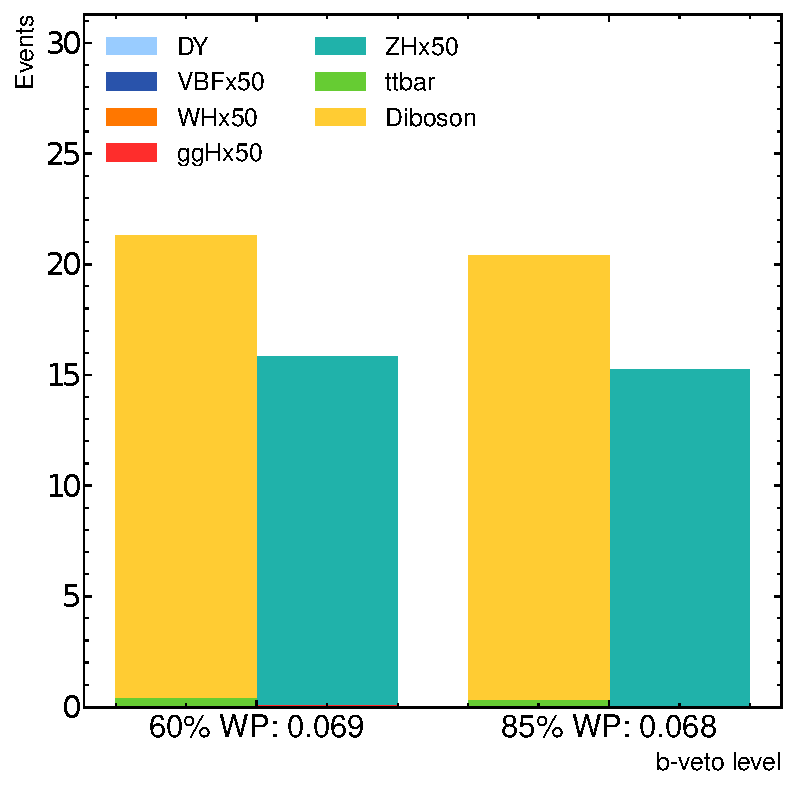
\includegraphics[width=0.4\textwidth]{figures/hmm/bveto/btag-4lep.pdf}}}
\subfloat[][]{{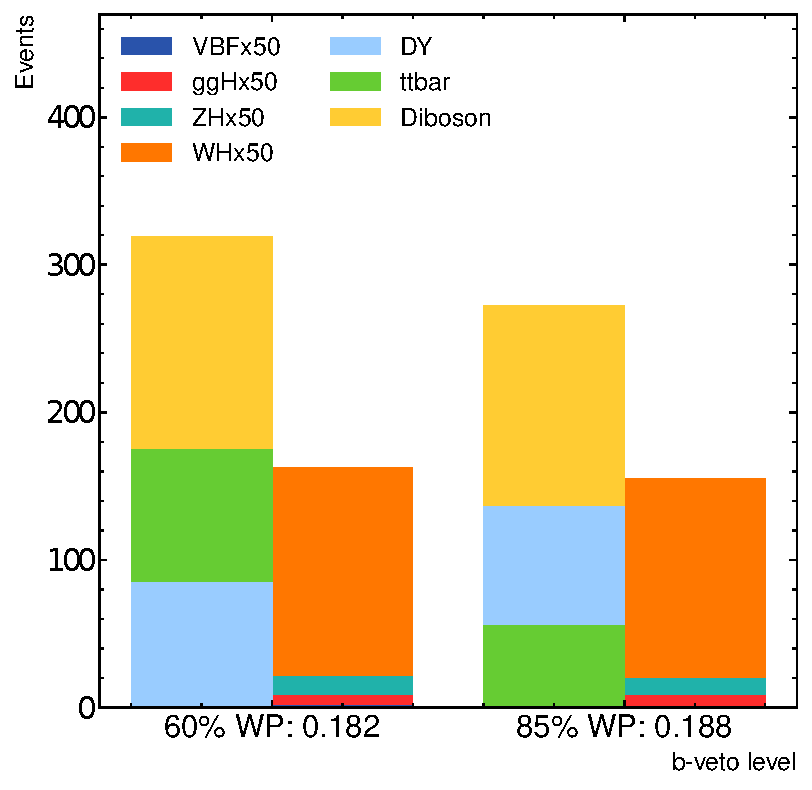
\includegraphics[width=0.4\textwidth]{figures/hmm/bveto/btag-3lep.pdf}}}
\caption{Illustration of the impact on signal and background yields of using different btag working points (WP) for the b-jet veto. This is shown for the 4-lepton selection (a) and 3-lepton selection (b). Each bar shown the number of simulated signal or background events passing the selection when using the WP marked on the x-axis. For both selections, using the looser 85\% WP reduces the background yields compared to the tighter 60\% WP. At the same time, the signal yield is relatively unchanged.}
\label{fig:hmmBveto}
\end{figure}

\begin{table}[ht!]
 \caption{Cutflow for 4-lepton and 3-lepton selection. Lepton pairs are opposite charge.}
 \begin{center}
\begin{tabular}{c c  c}\toprule
Step & 4-lepton & 3-lepton \\\midrule
1 & \multicolumn{2}{c}{No 85\% WP btag jets (b-jet veto)}           \\\midrule
2 & At least 4 leptons                                & Exactly 3 leptons\\\midrule
3 & ($N_{\mu^+}>$0 and $N_{\mu^-}>$0)                 & ($N_{\mu^+}>$0 and $N_{\mu^-}>$0) \\\midrule
4 & A dimuon pair $\exists\in$ [110,160] GeV                    & A dimuon pair $\exists\in$ [110,160] GeV \\\midrule
\multirow{2}{*}{5} & ($N_{\mu^+}>$1 and $N_{\mu^-}>$1) or              & ($N_{\mu^+}>$1 or $N_{\mu^-}>$1) or \\
  & ($N_{e^-}>$0 and $N_{e^+}>$0)                    & ($N_{e^-}>$0 or $N_{e^+}>$0)  \\\midrule
6 & $\nexists$ two Z$\to\mu\mu$ candidates                        & $\nexists$ Z$\to\mu\mu$ candidate  \\\midrule
7 & Higgs candidate $\in$ [110,160] GeV                  & Higgs candidate $\in$ [110,160] GeV \\\midrule
\multirow{2}{*}{8} & Kinematic cuts 27/15/8/6 GeV $>p_T$                    & Kinematic cuts 27/10/15(10) GeV $>p_T$ \\
  &                                                        & for $e(\mu)$ \\
\bottomrule\end{tabular}
 \end{center}
\label{tab:hmmEv}
\end{table}

The steps of the cutflow are shown in table \ref{tab:hmmEv}, which defines the 4-lepton and 3-lepton VH candidate categories.
This cutflow defines ``\Z candidates'' to be oppositely charged dimuon pairs an invariant-mass in $[80,105]$~GeV.
The selection of oppositely charged muons for the Higgs candidate, and of additional leptons for the \Z(\W) candidates is based on minimizing a $\chi^2$ calculation related to the invariant-mass (transverse-mass) and corresponding resolutions of the candidates.
This is shown in equations \ref{eq:hmmWhPairing} and \ref{eq:hmmZhPairing}.
Here, for each candidate pairing, $\chi^{2,\text{cand}}$ is calculated from the Higgs candidate mass $M_H^\text{cand}$.
For 4-lepton events, the \Z candidate mass $M_Z^\text{cand}$ is used, and for 3-lepton events the transverse-mass of the W candidate lepton and $E_T^\text{miss}$, $M_T^\text{cand}$, is used.
Only pairings with oppositely charged muons are considered for $M_H^\text{cand}$, while all oppositely charged same flavor pairs are considered for $M_Z^\text{cand}$.
Leptons of both flavors and charges are considered for $M_T^\text{cand}$.
The pairing with the smallest $\chi^{2,\text{cand}}$ is selected.

\begin{equation}
  \label{eq:hmmWhPairing}
  \chi^{2,\text{cand}}_{\W} = \frac{(M_H^\text{cand}-125\text{ GeV})^2}{(3.0\text{ GeV})^2} + \frac{(M_T^\text{cand}-70\text{ GeV} )^2}{(20\text{ GeV})^2}
\end{equation}

\begin{equation}
  \label{eq:hmmZhPairing}
  \chi^{2,\text{cand}}_{\Z} = \frac{(M_H^\text{cand}-125\text{ GeV})^2}{(3.0\text{ GeV})^2} + \frac{(M_Z^\text{cand}-91.1\text{ GeV} )^2}{(3.0\text{ GeV})^2}
\end{equation}

The $\chi^2$ pairing is used to improve the pairing efficiency.
Other pairing procedures were considered but were rejected based on their performance.
For example, in 4-muon events, selecting the highest $p_T$ opposite sign muon pair is 63.4\% less efficient than the $\chi^2$ pairing described above. 
Selecting the pair such that the \Z candidate is closest to the \Z mass is 8.7\% less efficient.

The cuts described in table \ref{tab:hmmEv} define two categories of events, 3-lepton and 4-lepton, which are referred to as inclusive categories in relation to the subsequent division into smaller categories.
The kinematic distributions of the leptons in these categories are illustrated in Section \ref{sec:hmmKine}.

\subsection{Simulation}\label{sec:hmmSim}

Simulated datasets play a central role in the search strategy.
All simulated datasets are scaled to match their corresponding cross-section \cite{higgsCross}.
First, the simulated background and signal datasets allow an exploration of the efficiency of various event selection criteria.
This eventually leads to the criteria listed in Table \ref{tab:hmmEv}.
Next, probability density distributions are constructed from simulated events that describe the probability to observe variables at a given value.
This is done both both for background and signal productions.
This allows the development of a multivariate discriminant function that separates signal and background events based on these variables.
% Simulated events are used at each step of this process: to determine the discriminant function with one set of simulated events and constrain the level of bias it may introduce with a second set of events.
% After this, an unrelated third set is used to estimate the rates of signal and background events, as a function of dimuon invariant mass, at different levels of discrimination.
The background rates as a function of \muu are used to measure systematic uncertainties and to validate the performance of several empirical background models.
The signal shape is used for these purposes as well, and most importantly, it provides the signal component in the hypothesis test performed on the observed data.
Finally, several theoretical and experimental variations on the signal shape are used to measure the impact of these uncertainties on the final result.

% Background ========================
The primary background production in the region of interest comes from Drell-Yan (DY), Diboson, and top production mechanisms described in section \ref{sec:phenoBkg}.
The dominant background mechanism, DY, primarily produces events with two leptons in the final state.
This is reduced through the requirement of more than two leptons in the event selection.
Processes involving $t\tbar$ and single-top production form a large background component as well.
Since the top quark always produces a bottom quark through decay, these backgrounds are mitigated by use of the b-jet veto in the event selection.
After this are diboson productions of $ZZ$ or $WZ$ with leptonic decays.
The diboson is topologically the most similar to the VH signal, making this the most challenging process to reject.
Diboson events are reduced with the help of a discriminant function based on several kinematic observables, but these events remain the dominant background after all selections are complete.

The DY simulations are generated with \sherpa 2.2.1 using the NNPDF3.0 PDF.
The DY \muu spectrum falls exponentially.
To generate sufficient numbers of high-mass events, these are simulated in ranges of $x$, where $x$ is the maximum of the mediator \pt and the scalar parton \pt sum, \httt.
These simulations are produced to NLO for diagrams, including fewer than three jets and LO for diagrams, including three or four jets.

The $t\tbar$ and single-top simulations are produced with \powheg v2 and the NNPDF3.0NLO PDF.
The mass of the top quark is set to $m_t=172.5$.
The $t\tbar$ cross section is calculated to NNLO using Top++2.0 \cite{Czakon:2011xx}.
The leading order $t\tbar$ Feynman diagrams are shown in Figure \ref{fig:phenoTtbar}.
The cross-sections of single-top production channels are calculated to NNLL accuracy following the standard procedure \cite{Kidonakis:2011wy, Kidonakis:2010ux}.
The leading order single-top Feynman diagrams are shown in Figure \ref{fig:phenoSingleTop}.
Different simulations are generated for $s$-channel and $t$-channel production through the exchange of a \W boson. A sample is produced for single-top production in association with a \W as well.

The final background simulations are composed of the diboson processes $WZ$ and $ZZ$ with leptonic decays.
These are produced with \sherpa 2.2.1 (for quark decays) and \sherpa 2.2.2 (for fully leptonic decays) and the NNPDF3.0 PDF.
Some number of fully or partially leptonic decays of the diboson final state are simulated in order to be considered as an additional background.
One set of simulations simulates $ZZ\to q\qbar\ll$ and $WZ\to q\qbar\ll$ events, while a second set simulates events with $\ll\ll$, $\ll\ell\nu$, and $\ll\nu\nu$ final states \cite{ATL-PHYS-PUB-2017-005}.
The purely leptonic $\ll\ll$ originates from two \Z decays.
This is the primary background in the 4-lepton categories and shares a very similar topology to ZH.
For completeness, the $ZZ$ decay to $\ll\nu\nu$ is simulated as well.
The production of $WZ$ $\ll\ell\nu$ is the primary background for several 3-lepton categories.
The leading order diboson Feynman diagrams are shown in Figure \ref{fig:phenoDiboson}.

% Signal simulations ========================
Signal simulations are produced based on the dominant Higgs production mechanisms listed in Table \ref{tab:higgsCrossSec}.
Most simulations are simulated with a Higgs mass set to 125~GeV using \powheg v2 and the PDF4LHC15 PDF. 
The exception is ttH, which is produced with \madgraph and the NNPDF3.0NLO PDF.
The precision ranges from NNLO in QCD for the ggF, to NLO for the VBF, VH, and ttH mechanisms.
The contribution of $gg\to ZH$ is simulated at LO.


\subsection{Kinematic Distributions}\label{sec:hmmKine}

The pre-cut categories defined in Section \ref{sec:hmmEv} are illustrated here with the aid of the simulated signal and background simulations.
The mass distributions are presented in Figure \ref{fig:hmmPrecutMassHists}.
These provide an illustration of the composition of the background and signal contributions to these categories, as well as the general agreement between data and simulation. 

\begin{figure}[h!]
\captionsetup[subfigure]{position=b}
\centering
\subfloat[][]{{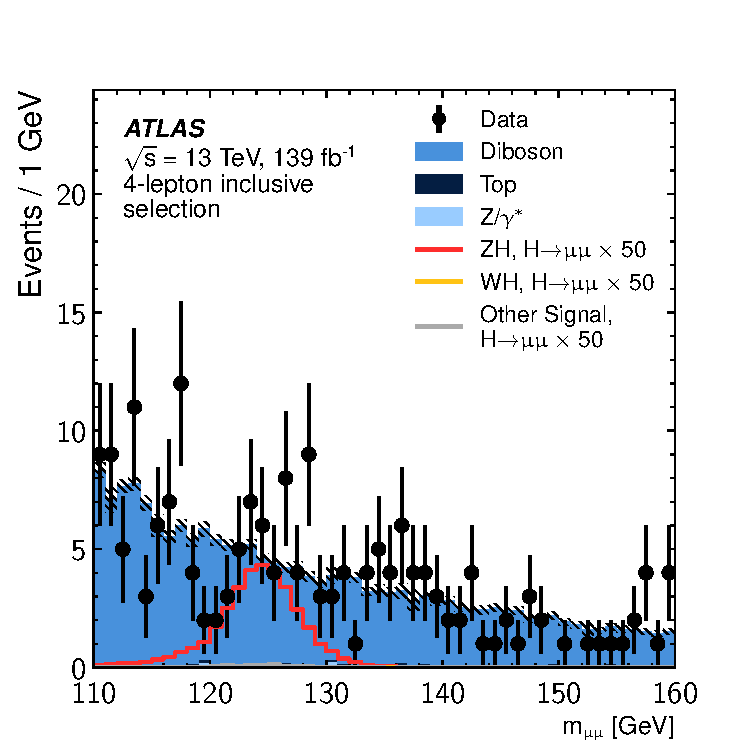
\includegraphics[width=0.5\textwidth]{figures/hmm/public/preCut/histo-4lep-muu.pdf}}} % public version of plots
\subfloat[][]{{\includegraphics[width=0.5\textwidth]{figures/hmm/public/preCut/histo-3lep-muu.pdf}}}
% \subfloat[][]{{\includegraphics[width=0.5\textwidth]{figures/hmm/preCut/histo-4lep-muu.pdf}}}
% \subfloat[][]{{\includegraphics[width=0.5\textwidth]{figures/hmm/preCut/histo-3lep-muu.pdf}}}
\caption{Distributions of \muu in the 4-lepton (left) and 3-lepton (right) categories. The binning is adjusted based on the multiplicities of the categories. The signal distributions, shown in colored lines, are scaled by a factor of 50 for visibility.}
\label{fig:hmmPrecutMassHists}
\end{figure}

    
Other kinematic distributions ($p_T$, $\eta$, $\phi$) for the selected leptons are illustrated in Figures \ref{fig:hmmKineWhMuons} to \ref{fig:hmmKineZhLeps}.
The muon candidates for the Higgs are called $\mu^1$ and $\mu^2$ in descending order of $p_T$. 
Likewise, for the 4-lepton category, the selected leptons for the Z candidate are named $\ell^1$ and $\ell^2$ again in descending order of $p_T$.



\clearpage
\begin{figure}[htpb]
  \centering
  \includegraphics[width=0.4\textwidth]{figures/hmm/kinematics/histo-3lep-u1_pt.pdf}
  \includegraphics[width=0.4\textwidth]{figures/hmm/kinematics/histo-3lep-u2_pt.pdf}
  \includegraphics[width=0.4\textwidth]{figures/hmm/kinematics/histo-3lep-u1_eta.pdf}
  \includegraphics[width=0.4\textwidth]{figures/hmm/kinematics/histo-3lep-u2_eta.pdf}
  \includegraphics[width=0.4\textwidth]{figures/hmm/kinematics/histo-3lep-u1_phi.pdf}
  \includegraphics[width=0.4\textwidth]{figures/hmm/kinematics/histo-3lep-u2_phi.pdf}
  \caption{Kinematic plots showing $p_T$, $\eta$, and $\phi$ distributions for the H candidate muons from the 3-lepton selection.}
    \label{fig:hmmKineWhMuons}
\end{figure}

\clearpage
\begin{figure}[htpb]
  \centering
  \includegraphics[width=0.4\textwidth]{figures/hmm/kinematics/histo-3lep-aux1_pt.pdf}\\
  \includegraphics[width=0.4\textwidth]{figures/hmm/kinematics/histo-3lep-aux1_eta.pdf}\\
  \includegraphics[width=0.4\textwidth]{figures/hmm/kinematics/histo-3lep-aux1_phi.pdf}\\
  \caption{Kinematic plots showing $p_T$, $\eta$, and $\phi$ distributions for the additional lepton/W candidate for the 3-lepton selection.}
    \label{fig:hmmKineWhLeps}
\end{figure}

\clearpage
\begin{figure}[htpb]
  \centering
  \includegraphics[width=0.4\textwidth]{figures/hmm/kinematics/histo-4lep-u1_pt.pdf}
  \includegraphics[width=0.4\textwidth]{figures/hmm/kinematics/histo-4lep-u2_pt.pdf}
  \includegraphics[width=0.4\textwidth]{figures/hmm/kinematics/histo-4lep-u1_eta.pdf}
  \includegraphics[width=0.4\textwidth]{figures/hmm/kinematics/histo-4lep-u2_eta.pdf}
  \includegraphics[width=0.4\textwidth]{figures/hmm/kinematics/histo-4lep-u1_phi.pdf}
  \includegraphics[width=0.4\textwidth]{figures/hmm/kinematics/histo-4lep-u2_phi.pdf}
  \caption{Kinematic plots showing $p_T$, $\eta$, and $\phi$ distributions for the H candidate muons from the 4-lepton selection.}
    \label{fig:hmmKineZhMuons}
\end{figure}

\clearpage
\begin{figure}[htpb]
  \centering
  \includegraphics[width=0.4\textwidth]{figures/hmm/kinematics/histo-4lep-aux1_pt.pdf}
  \includegraphics[width=0.4\textwidth]{figures/hmm/kinematics/histo-4lep-aux2_pt.pdf}
  \includegraphics[width=0.4\textwidth]{figures/hmm/kinematics/histo-4lep-aux1_eta.pdf}
  \includegraphics[width=0.4\textwidth]{figures/hmm/kinematics/histo-4lep-aux2_eta.pdf}
  \includegraphics[width=0.4\textwidth]{figures/hmm/kinematics/histo-4lep-aux1_phi.pdf}
  \includegraphics[width=0.4\textwidth]{figures/hmm/kinematics/histo-4lep-aux2_phi.pdf}
  \caption{Kinematic plots showing $p_T$, $\eta$, and $\phi$ distributions for the Z candidate leptons from the 4-lepton selection.}
    \label{fig:hmmKineZhLeps}
\end{figure}
\clearpage



\section{Multivariate Categorization}\label{sec:hmmBdt}

The events belonging to the inclusive 3-lepton and 4-lepton categories are further divided into exclusive sub-categories.
The definition of the exclusive categories is based on a multivariate discriminant that is a function of several kinematic variables.
The discriminant for classification is calculated using a \emph{boosted decision tree} (BDT).
This is a function of event kinematics that is defined to identify signal-like events from the larger set of background-like events.
It is derived based on the available information about signal and background kinematics from simulation.
This derivation, or \emph{training}, is performed by fitting the free parameters of the BDT to the available information.

\begin{figure}[h!]
\captionsetup[subfigure]{position=b}
\centering
\subfloat[][]{\label{fig:bdtTree}{\includegraphics[scale=0.35]{figures/hmm/tree.pdf}}}
\subfloat[][]{{\includegraphics[scale=0.35]{figures/hmm/ensamble.pdf}}}
\caption{Figure (a) schematizes an individual decision tree, where in boolean splits based on the value of variables $v$ result in a categorization of signal or data as output. In a CART, the output is replaced by a continuous weight encoding ``signal-like'' versus ``background-like''. Figure (b) schematizes an ensemble of trees with different topologies, each defining an output function.}
\label{fig:}
\end{figure}

The information available for the training consists of datasets of $n$ entries and $m$ variables
The multi-dimensional entries $x_i$ $i\in[1,...,n]$ are labeled as either signal or background with $y_i$.
The elements of $x_i$ are variables $v_j$ $j\in[1,...,m]$.
The BDT is composed by of ensemble of decision trees.
A decision tree maps an entry of the dataset $x_i$ onto a discrete output space, such as a signal-vs-background likelihood.
Each node of the tree may represent a binary decision, or split, based on the variables of the entry.
Alternatively, the nodes with no children (leaves) may represent a decision, as illustrated in Figure \ref{fig:bdtTree}.
A generalization of a decision tree that assigns continuous weights to each leaf is a classification and regression tree (CART).
A tree can be \emph{trained} to map a set of input entries $x_i$ onto their corresponding labels $y_i$ by treating the distributions of input variables as PDFs and selecting splits (a, b, ...) that result in the highest output fidelity.
A single CART tends to struggle to represent the complexity of simulated physics datasets succinctly.
This performance can be augmented by an ensemble of CARTs labeled $k$, each with an output function $f_k(x_i)$ as illustrated in Figure \ref{fig:bdtTree}.
The output functions act as a \emph{model} of the provided dataset.
The sum of the CART output functions defines a new ensemble output function $f(x_i)=\hat{y}_i$, also called the discriminant score.

The training strategy is to develop an ensemble whose output functions accurately predict the corresponding label $y_i$ for unseen events.
This is quantified by a regularized loss function,
\begin{equation}\begin{split}\label{eqn:lossFunc}
    \mathcal{L}(\phi)=\sum_i l(\hat{y}_i,y_i),
\end{split}\end{equation} 
where $l$ measures the difference between $\hat{y}_i$ and $y_i$.
A process is defined to select trees, splits, and weights to minimize Equation \ref{eqn:lossFunc}.

The algorithm of \emph{boosting} is employed to minimize such loss functions by improving on the capability of a single CART.
It consists of iteratively expanding an ensemble of trees, with each addition addressing the mis-categorization of the previous ensemble.
One algorithm, \code{AdaBoost}, performs this task by iteratively reweighting poorly categorized entries to be more important to the following tree.
Another algorithm, \code{Gradient Boosting}, instead adds trees that are trained on the previous ensemble's poorly categorized entries.
Both of these algorithms played a role in the development of the analysis.
A descendent of \code{AdaBoost} and \code{Gradient Boosting} is \xgb, which introduces a modified loss function,
\begin{equation}\begin{split}\label{eqn:lossFuncXgb}
    \mathcal{L}(\phi)=\sum_i l(\hat{y}_i,y_i)+\sum_k \Omega(f_k).
\end{split}\end{equation} 
In Equation \ref{eqn:lossFuncXgb}, $\Omega$ is a measure of the complexity a tree.
The \xgb algorithm iteratively adds trees of diminishing weights, shrinking their importance by a constant factor.
It also introduces procedures to more quickly add and remove branches from trees while fitting the loss function.
These result in an accurate and reliable output function that can be trained quickly.
The \xgb algorithm was selected to construct the multivariate discriminant functions that are used in this analysis.
\cite{xgboost}

% Overtraining
It is a general goal to understand the underlying probability distributions that have produced a dataset, rather than of the dataset itself.
This applies to tasks such as training BDTs to discriminate signal from background, as well as fitting a functional form to data to model a background distribution. 
In both cases, the analytic model is interpreted as knowledge of these underlying distributions.
When solving an optimization problem such as those posed in Equations \ref{eqn:lossFunc} and \ref{eqn:lossFuncXgb}, the minimization algorithm has only the dataset at its disposal.
This can lead to \emph{over-training} or \emph{over-fitting}, where the optimization of the loss function tunes the discriminant to the features of a particular dataset rather than the features of the underlying distributions.
This problem tends to grow in step with the complexity of the model.
It is combatted, in part, by penalizing the optimization by the complexity of the model; the $\Omega$ function of Equation \ref{eqn:lossFuncXgb} is one such example.

Over-training may have two important and detrimental effects.
The first is to reduce the efficacy of the discriminant when applied to a new dataset.
Although this impacts the performance of the analysis, it does not necessarily invalidate the results by the introduction of bias.
The greater danger to the integrity of the analysis arises when the performance of the discriminant is inaccurately measured.
This second effect is illustrated in the following example.
Suppose a BDT is trained to identify signal events from a simulated dataset, and the same dataset is used to predict the number of signal events to expect in observed data.
A signal-rich category is defined based on the discriminant score for events.
In this case, simulated signal events tend to be over-represented in the category.
The BDT will identify simulated signal events with higher efficiency compared to signal in the data, leasing to an unconstrained uncertainty on the expected signal.
Unlike the first effect, this type of error invalidates the double use of the training simulation for further measurements.

\begin{figure}[h!]
\captionsetup[subfigure]{position=b}
\centering
\includegraphics[width=0.75\textwidth]{figures/hmm/testTrainVal.pdf}
\caption{The top row, $p_0$, shows an schematization of a dataset divided into five subsets with $k$-fold split with $k=5$.
The blue boxes represent sets to be used for training, the green boxes for validation, the red boxes for testing.
Five permutations of these assignments, $p_i$, are shown for the same dataset.
In cross-validation, a separate MVA is fit to each permutation, such that each entry of the full dataset belongs to the testing set for a particular MVA.
}
\label{fig:testTrainVal}
\end{figure}

The problem of over-training is mitigated by introducing a $k$-fold split of the available simulated datasets into a number, $k>2$, of subsets of similar multiplicity.
One subset is labeled as the ``testing'' set, and another is labeled as a ``validation'' set.
The remaining subsets are combined as a ``training'' set.
This is illustrated in the top of Figure \ref{fig:testTrainVal}.
The BDT algorithm is deployed on the training set, and further predictions with respect to the simulation are performed with the testing set.
Since the testing set has not been exposed to the BDT during training, there is no direct risk of over-training of the discriminant scores in the testing set.
There remains the issue of selecting thresholds that define the signal-rich category to optimize, for example, the expected sensitivity.
This choice is subject to the same concerns about over-training as the selection of trees during the training phase. 
A third set, the validation set, is defined orthogonally to both the training and testing sets.
This set is used to study the convergence of the training process, check for over-training effects that may reduce sensitivity, and, most importantly, to choose the discriminant thresholds for further categorization.

The final consideration is to inefficiency that such a division of the simulation set entails.
Simulated events are computationally expensive to produce.
A \emph{cross-validation} scheme calls for the permutation of each of the $k$ subdivisions, such that each event appears once in a test set, available for further analysis.
This is shown in Figure \ref{fig:testTrainVal}.
A separate BDT is trained with the training set from each permutation.
This means that each event in the full dataset has one discriminant score from a BDT for which it is in the testing set, one for which it is in the validation set, and $k-2$ for which it was in the training set.
The scores from the BDT for which an event was in the testing and validation sets are the testing and validation scores, respectively.

\subsection{Configuration}
\label{sec:hmmBdtConfiguration}

% Training details
Separate classifiers are trained for 3-lepton and 4-lepton categories, but there are many similarities between these.
A 5-fold splitting of the available signal and background simulation is used.
It is important to note that the testing set remains blinded until all choices related to the categorization channels have been fixed.
The output of the BDT on the testing set is final, and it is essential to refrain from making choices related to the procedure based on the testing set.
A cyclic permutation of the 5-fold splitting is used, such that a separate BDT is trained for each fifth of the total simulation.

% Samples
Each BDT is trained using the simulated background, in which all background components are included.
The signal for the 4-lepton BDTs are the qqZH samples, while the signal for the 3-lepton BDTs are the W$^\pm$H samples.
The per-event weights arising from scale factors and reweighing, along with the event corresponding to the campaign luminosity, cross-section, are provided to the BDT.
Negatively weighted events are removed, and the signal and background weights are both normalized.
% Sample statistics
The numbers of available simulated events for training are shown in table \ref{tab:hmmSampleStatistics}.

\begin{table}[htbp]
 \caption{Numbers of simulated events available for training, both in the full simulation, and the 3/5 training sets statistics.}
 \begin{center}
\begin{tabular}{l r r r}\toprule
Simulation           & Total Events & Training Events \\
\midrule
4-lepton signal      & 20700        & 12508    \\
4-lepton background  & 88314        & 53081    \\
3-lepton signal      & 134936       & 80962    \\
3-lepton background  & 185286       & 111107   \\
\bottomrule\end{tabular} 
 \end{center}
\label{tab:hmmSampleStatistics}
\end{table}

% Training variables
The set of variables provided as input for the BDT was chosen from a broader set of candidate variables with physical motivations.
This set was reduced in the order of ascending \emph{feature importance}, defined as the number of times the variable is used for a decision node, weighted by the number of events categorized by the node during training.
The reduction continued until the performance of the BDT began to decline.
Different variables are defined based on the different final state topologies in the inclusive 4-lepton and 3-lepton categories.
The variables for each are listed in Table \ref{tab:hmmVarNames}.

\begin{table}[htp]
\caption{Variable names and definitions used training the 3-lepton ($3\ell$) and 4-lepton ($4\ell$) BDTs. The second column indicates the BDT in which the variable was used, based on the lepton category number.}
\begin{center}
\begin{tabular}{l c l l}
\toprule
Variable & Used for BDT & Definition \\
\midrule
  $m_T(E_T^\text{miss},l1)$ & $3\ell$ & Transverse mass of the W candidate lepton and $E_T^\text{miss}$  \\
  $\Delta_\phi(E_T^\text{miss},H)$ & $3\ell$ & $\phi$ between $E_T^\text{miss}$ and the H candidate \\
  $E_T^\text{miss}$ & $3\ell$ & Missing transverse momentum \\
  $p_T^{l1}$ & $3\ell$ & W candidate lepton $p_T$ \\
  $\Delta_\phi(l1,H)$ & $3\ell$ & $\Delta$ $\phi$ between H candidate and W candidate lepton \\
  $\Delta_\eta(l1,H)$ & $3\ell$ & $\Delta$ $\eta$ between H candidate and W candidate lepton \\
  $p_T^{j1}$ & $3\ell$ and $4\ell$ & $p_T$ of leading jet (if present) \\
  $N_\text{jets}$ & $3\ell$ and $4\ell$ & Number of jets \\
  $p_T^{j2}$ & $4\ell$ & $p_T$ of subleading jet (if present) \\
  $\Delta_\phi(l1,l2)$ & $4\ell$ & $\Delta$ $\phi$ between the leptons paired for the Z candidate \\
  $\Delta_\phi(Z,H)$ & $4\ell$ & $\Delta$ $\phi$ between H candidate and Z candidate \\
  $\Delta_\eta(Z,H)$ & $4\ell$ & $\Delta$ $\eta$ between H candidate and Z candidate \\
  $m_Z$ & $4\ell$ & Z candidate mass \\
\bottomrule
\end{tabular}
\label{tab:hmmVarNames}
\end{center}
\end{table}


\afterpage{
\begin{figure}[h!]
\captionsetup[subfigure]{position=b}
\centering
\subfloat[][]{{\includegraphics[width=0.35\textwidth]{figures/hmm/public/kine/kine-3lep-aux1_met_mt.pdf}}}
\subfloat[][]{{\includegraphics[width=0.35\textwidth]{figures/hmm/public/kine/kine-3lep-aux1_pt.pdf}}}
\subfloat[][]{{\includegraphics[width=0.35\textwidth]{figures/hmm/public/kine/kine-3lep-aux1_uu_delta_eta.pdf}}} \\
\subfloat[][]{{\includegraphics[width=0.35\textwidth]{figures/hmm/public/kine/kine-3lep-aux1_uu_delta_phi.pdf}}}
\subfloat[][]{{\includegraphics[width=0.35\textwidth]{figures/hmm/public/kine/kine-3lep-j1_pt.pdf}}}
\subfloat[][]{{\includegraphics[width=0.35\textwidth]{figures/hmm/public/kine/kine-3lep-met_pt.pdf}}} \\
\subfloat[][]{{\includegraphics[width=0.35\textwidth]{figures/hmm/public/kine/kine-3lep-met_uu_delta_phi.pdf}}}
\subfloat[][]{{\includegraphics[width=0.35\textwidth]{figures/hmm/public/kine/kine-3lep-nJets.pdf}}}
\caption{Training variables provided as input for the for the 3-lepton classifier. The signal distribution shown in red is comprised of the simulated WH signal dataset, while the background distribution contains all background production modes shown in blue. Data distributions are included in black. Each distribution is normalized, and the error bars on each histogram are statistical only. }
\label{fig:hmm3lepVars}
\end{figure}
\clearpage
}

\afterpage{
\begin{figure}[h!]
\captionsetup[subfigure]{position=b}
\centering
\subfloat[][]{{\includegraphics[width=0.35\textwidth]{figures/hmm/public/kine/kine-4lep-auxDilep_delta_phi.pdf}}}
\subfloat[][]{{\includegraphics[width=0.35\textwidth]{figures/hmm/public/kine/kine-4lep-auxDilep_mass.pdf}}}
\subfloat[][]{{\includegraphics[width=0.35\textwidth]{figures/hmm/public/kine/kine-4lep-aux_uu_delta_eta.pdf}}} \\
\subfloat[][]{{\includegraphics[width=0.35\textwidth]{figures/hmm/public/kine/kine-4lep-aux_uu_delta_phi.pdf}}}
\subfloat[][]{{\includegraphics[width=0.35\textwidth]{figures/hmm/public/kine/kine-4lep-j1_pt.pdf}}}
\subfloat[][]{{\includegraphics[width=0.35\textwidth]{figures/hmm/public/kine/kine-4lep-j2_pt.pdf}}} \\
\subfloat[][]{{\includegraphics[width=0.35\textwidth]{figures/hmm/public/kine/kine-4lep-nJets.pdf}}}
\caption{Training variables provided as input for the for the 4-lepton classifier. The signal distribution shown in red is comprised of the simulated ZH signal dataset, while the background distribution contains all background production modes shown in blue. Data distributions are included in black. Each distribution is normalized, and the error bars on each histogram are statistical only. }
\label{fig:hmm4lepVars}
\end{figure}
\clearpage
}


%%%%%%%%%%%% Variable importance

% \begin{figure}[htpb]
%   \centering
%   \includegraphics[height=0.48\textwidth]{figures/hmm/nJets/histo-3lep-nJets.pdf}
%   \includegraphics[height=0.48\textwidth]{figures/hmm/zCand/histo-4lep-auxDilep_mass.pdf}
%   \caption{Left: N Jets distribution for 3-lepton channel, right: Z candidate mass for 4-lepton channel. These are the highest ranked in feature importance for their category's respective BDT's.}
%     \label{fig:hmmImpVars}
% \end{figure}

The feature importances for each training case are listed in Tables \ref{tab:3lepVarImport} and \ref{tab:4lepVarImport}.
In the 4-lepton case, the most important variable is the mass of the \Z candidate, which helps identify the signal.
In the 3-lepton case, the most important variable is the number of jets, which helps especially to separate out top quark backgrounds.

% \begin{figure}[htpb]
%   \centering
%   \includegraphics[height=8cm]{figures/hmm/bdtImportance/imp-4lep.pdf}
%   \includegraphics[height=8cm]{figures/hmm/bdtImportance/imp-3lep.pdf}
%   \caption{The 4-lepton (left) and 3-lepton (right) variables shown with their respective feature importance, averaged over the five BDTs trained for each cross-validation permutation. The importance of a variable is defined relative to the other variables.}
%     \label{fig:hmmVarImport}
% \end{figure}

\afterpage{
\begin{table}[htp]
\caption{Feature importance for the 3-lepton BDTs. The values shown are the feature importances normalized to the highest-importance variable. Values are given for individual BDTs along with a combined weight based on the sum across BDTs. The most important variable is the jet multiplicity.}
\begin{center}
\begin{tabular}{l ccccccc}
\toprule
Variable & BDT1 & BDT2 & BDT3 & BDT4 & Combined \\
\midrule
N Jets & 1.00 & 1.00 & 1.00 & 1.00 & 1.00 \\
$p_T^{j1}$ & 0.38 & 0.42 & 0.34 & 0.31 & 0.36 \\
$\Delta_\eta(l1,H)$ & 0.16 & 0.18 & 0.16 & 0.15 & 0.17 \\
$p_T^{l1}$ & 0.12 & 0.13 & 0.14 & 0.13 & 0.14 \\
$E_T^\text{miss}$  & 0.14 & 0.13 & 0.13 & 0.12 & 0.13 \\
$\Delta_\phi(E_T^\text{miss},H)$ & 0.09 & 0.08 & 0.10 & 0.10 & 0.09 \\
$m_T^{l1,E_T^\text{miss}}$ & 0.08 & 0.09 & 0.09 & 0.09 & 0.09 \\
$\Delta_\phi(l1,H)$ & 0.08 & 0.06 & 0.06 & 0.07 & 0.08 \\
\bottomrule
\end{tabular}
\label{tab:3lepVarImport}
\end{center}
\end{table}
%
\begin{table}[htp]
\caption{Feature importance for the 4-lepton BDTs, in the format of table \ref{tab:3lepVarImport}. The most important variable is the \Z candidate mass.}
\begin{center}
\begin{tabular}{l ccccccc}
\toprule
Variable & BDT1 & BDT2 & BDT3 & BDT4 & Combined \\
\midrule
$m_Z$ & 1.00 & 0.79 & 0.67 & 0.78 & 1.00 \\
N Jets & 0.99 & 1.00 & 1.00 & 1.00 & 0.89 \\
$p_T^{j1}$ & 0.78 & 0.44 & 0.19 & 0.25 & 0.60 \\
$\Delta_\eta(Z,H)$ & 0.45 & 0.39 & 0.37 & 0.51 & 0.55 \\
$p_T^{j2}$ & 0.12 & 0.41 & 0.49 & 0.58 & 0.31 \\
$\Delta_\phi(l1,l2)$ & 0.30 & 0.19 & 0.18 & 0.23 & 0.29 \\
$\Delta_\phi(Z,H)$ & 0.28 & 0.19 & 0.19 & 0.21 & 0.23 \\
\bottomrule
\end{tabular}
\label{tab:4lepVarImport}
\end{center}
\end{table}
\clearpage
}

The performance of a BDT is measured using the validation scores of the receiver operator curve (ROC).
The ROC is a parametric function of the BDT discriminant, plotted as the rate of correct signal categorizations (true positive rate) compared to the rate of false categorization of background as signal (false positive rate).
This is plotted in Figure \ref{fig:hmmBdtRoc} for a number of discriminant thresholds that define signal versus background.
A figure of merit used to evaluate the ROC is area-under-curve (AUC).
These show comparable performance for the BDTs of both categories and the impact of the relatively limited statistics of the 4-lepton sample.
As a cross check, the ROC curve for the training set is plotted along with the validation set. The agreement between these, within statistical uncertainty, does not indicate clear over-training effects.
The signal and background samples shown in the ROC plots correspond to the same samples used for the training; only WH and ZH signals are used in the definition of the ROC.

\begin{figure}[htpb]
  \centering
  \includegraphics[width=0.48\textwidth]{figures/hmm/bdtHist/roc-4lep-ZH-AllBackground-0-depth2-nEst80tag-new-AllBackground.pdf}
  \includegraphics[width=0.48\textwidth]{figures/hmm/bdtHist/roc-3lep-WH-AllBackground-0-depth2-nEst50tag-new-AllBackground.pdf}
  \caption{4 lepton (left) and 3 lepton (right) ROC curves for representative BDT's. Shown in black is the curve for the training set, while red shows the curve for the validation set (labeled test set). Error bars are statistical uncertainties due to the size of the training and validation datasets. The AUC is labeled on each plot.}
    \label{fig:hmmBdtRoc}
\end{figure}

% Figure \ref{fig:hmmBdtScoreLin} shows distributions of the BDT discriminant for different categories of signal and background, scaled the samples cross-section and luminosity.
% The signal/background separation is more apparent in this plot than in those normalized to the physical expectation.


% \begin{figure}[htpb]
%   \centering
%   \includegraphics[width=0.48\textwidth]{figures/hmm/bdtHist/bar20-4lep-ZH-AllBackground-0-depth2-nEst80tag-new-AllBackground.pdf}
%   \includegraphics[width=0.48\textwidth]{figures/hmm/bdtHist/bar20-3lep-WH-AllBackground-0-depth2-nEst50tag-new-AllBackground.pdf}
%   \caption{4 lepton (left) and 3 lepton (right) distributions of the BDT discriminant, where the signal and background samples share a normalization. The signal distribution is that of the sample used for training, not the full signal MC sample.}
%     \label{fig:hmmBdtScoreLin}
% \end{figure}

Figure \ref{fig:hmmBdtScore} shows the BDT discriminant calculated in different categories and scaled by the samples cross-section and luminosity.
The signal and background composition is more apparent in these plots: primarily, the target signal production mechanism is separated from other signals.
The top backgrounds are particularly well separated owing in part to the high statistics available for these samples in the training sets.

% {\color{red} This paragraph section is slightly redundant. Merge into next section?}
% Exclusive categories are defined based on discriminant cuts that produce varying levels of signal purity.
% The category ``4-lepton high-purity'' is defined in the 4-lepton selection by requiring 4-lepton BDT score greater than 0.12. 
% Two categories are defined from the 3-lepton selection: ``3-lepton high-purity'' and ``3-lepton middle-purity''. 
% The former is selected by requiring 3-lepton BDT score greater than 0.7,
% and the latter is selected by requiring 3-lepton BDT score less than 0.7
% but greater than 0.1.
% The events failing VH categorization are still considered in the inclusive categories.
 
\begin{figure}[htpb]
  \centering
  \includegraphics[width=0.48\textwidth]{figures/hmm/public/bdt/histo-4lep-bdtScore.pdf}
  \includegraphics[width=0.48\textwidth]{figures/hmm/public/bdt/histo-3lep-bdtScore.pdf}
  \caption{4-lepton (left) and 3-lepton (right) distributions of the BDT discriminant, using the final test scores. The simulated background is shown in shaded grey, while the signal distributions are drawn as lines in red for ZH and orange for WH. The remaining non-VH production mechanisms (ggF, VBF, and ttH) are combined and plotted as a dark grey line. All the signal histograms have been scaled by a factor of 50 to enhance visibility.\\
  It is observed that the score separates the signal to the left and background to the right. Of similar importance is that it specifically isolates the VH signal of interest and not the other signal productions. For 4-lepton this is the ZH signal and for 3-lepton this is the WH signal. Vertical dotted lines indicate the values that delineate which events belong in which final categories. The full dataset is included as well, which is used to fix the normalization of the background. \\
  The 3-lepton discriminant separates signal from background to a higher degree than does the 4-lepton discriminant. This is due in part to the stricter 4-lepton event selection, which can remove many more ``easily'' separable background events. The remaining events are more similar, topologically, to the ZH signal.}
    \label{fig:hmmBdtScore}
\end{figure}

\subsection{Categorization}

The event selection results in two inclusive categories distinguished by lepton number: the 4-lepton and 3-lepton categories.
These selections are further divided into \emph{exclusive} categories based on the relative purity of the signal.
This subsequent division is based on the BDT discriminant scores for each event.
The 4-lepton category is divided once into low-purity and high-purity categories.
The 3-lepton category, with a greater event multiplicity, is divided into low-, medium-, and high-purity categories.

Each event belongs to both a validation dataset and a testing dataset, each of which has an associated discriminant score.
The validation scores are considered when selecting the score thresholds delineating categories.
The testing scores are used for the final hypothesis test and limit setting.
An optimization scan over various thresholds of the expected significance determines the threshold values.
The thresholds are selected in order to produce the highest expected significance, based on the validation scores.
These thresholds are specified in Table \ref{tab:hmmBdtCuts}.

\begin{table}[htp]
\caption{Category definitions based on the ranges of the discriminant value $O$. The output of the BDT is scaled such that $O\in[0,1]$, with higher numbers corresponding to VH-like events.}
\begin{center}
\begin{tabular}{c c c l l l}
\toprule
Inclusive Category & Exclusive Category & Criteria \\
\midrule
\multirow{2}{*}{4-Lepton} & High-purity & $O\ge0.12$ \\
                          & Low-purity & $O<0.12$ \\
\midrule
\multirow{3}{*}{3-Lepton} & High-purity & $O\ge0.72$ \\
                          & Middle-purity & $0.10\ge O<0.72$ \\
                          & Low-purity & $O<0.10$ \\
\bottomrule
\end{tabular}
\label{tab:hmmBdtCuts}
\end{center}
\end{table}

To first choose the thresholds using the testing set and then perform a hypothesis test in categories defined by that threshold would lead to a misleading signal and background expectation in those categories.
The choice of threshold would be biased to the statistical fluctuations in the test dataset.
This results in categories biased to contain more simulated signal events and fewer simulated background events than would be expected in the data.
Since the analysis of the data includes the signal model based on simulation, such a method is unacceptable.

\begin{figure}[htpb]
  \centering
  \includegraphics[width=0.45\textwidth]{figures/hmm/public/postCut/histo-4lep0-muu.pdf} \\
  \includegraphics[width=0.45\textwidth]{figures/hmm/public/postCut/histo-3lep0-muu.pdf} 
  \includegraphics[width=0.45\textwidth]{figures/hmm/public/postCut/histo-3lep1-muu.pdf} 
\caption{Distributions of \muu in the 4-lepton (top) and 3-lepton (bottom) selections after categorization based on a cut on the BDT discriminant score.}
    \label{fig:hmmPostcutMassHists}
\end{figure}
\clearpage

The high and middle-purity categories are considered for further analysis.
The low-purity events, containing few expected signal events, are only analyzed in the inclusive categories defined prior to BDT cut.
The distributions of \muu are shown in Figures \ref{fig:hmmPrecutMassHists} and \ref{fig:hmmPostcutMassHists}.
The former shows the inclusive distribution before further categorization with the BDT discriminant.
The latter shows the distributions in the categories defined in Table \ref{tab:hmmBdtCuts}.
The motivation to use the discriminant becomes apparent in these plots when compared to Figure \ref{fig:hmmPrecutMassHists}.
In both the 4-lepton and 3-lepton high-purity categories, Drell-Yan production has been virtually removed.
The background remaining is primarily from diboson sources.
The signal selection purity is also evident in the high-purity categories: these produce homogeneous selections of events from ZH or WH productions, depending on their target.


\section{Background Modeling}\label{sec:hmmBkg}

The results of this analysis are based on a comparison between signal and background hypotheses.
The simulated background distributions provide a powerful tool to understand the composition and kinematics of the backgrounds in each category.  
These also provide a possible definition for a background hypothesis, but this definition imports many theoretical assumptions.
Instead, an analytic background is developed from the data by fitting a functional form to the observation.

The Figures \ref{fig:hmmPrecutMassHists} and \ref{fig:hmmPostcutMassHists} show the \muu shapes of the simulated background distributions in the pre-cut and post-cut categories respectively.
In all cases, the background is characterized by a steeply falling \muu distribution with substantial contributions from \Z processes.
This motivates the inclusion of a Breit-Wigner shape in the functional form with the parameters of the \Z boson.
It is also important for the form to be flexible enough to describe the underlying background distribution without being flexible enough to describe the observed dataset's statistical fluctuations.
This motivates the inclusion of an exponential term that introduces only one flexible parameter.
The function chosen is defined in Equation \ref{eqn:hmmBkgFunc}. 
\begin{equation}\begin{split}\label{eqn:hmmBkgFunc}
    f_\text{B}(\muu) = (1-a)\times [f_{\text{BW},Z}\otimes\text{Gaus}()]+a\times\exp{b\times\frac{\muu-110\text{ GeV}}{160\text{ GeV}}}
\end{split}\end{equation} 
Here, \muu is the invariant-mass of the Higgs candidate dimuon, in GeV.
The Breit-Wigner function, $f_{\text{BW},Z}$ (defined in Equation \ref{eqn:breitWigner}), uses the \Z mass $m_\text{BW}=91.2$~GeV and width $\Gamma_\text{BW}=2.49$~GeV.
It is convolved with a Gaussian, the product of which is a Voigtian shape.
The Gaussian helps describe detector resolution effects and is centered at \muu with a width 2~GeV.
Two parameters are left to be determined by their agreement to the data.
The first, $a\in[0,1]$, represents the fraction of the background made of Breit-Wigner compared to the exponential term.
The second, $b$, determines the decent of the exponential term.
Equation \ref{eqn:hmmBkgFunc} is used to define a probability density function (PDF) over \mll from which observed events may have been sampled. 
When it is used to model the dataset, the PDF is normalized to the number of events in the dataset by a coefficient.
Since this coefficient is a function of $a$ and $b$, and it does not impact the shape of the distribution, it is suppressed.

The procedure to determine the free parameters is referred to as \emph{fitting} the functional form to the observed data.
The \code{minuit} algorithm \cite{roofit} is used to adjust the free parameters in order to maximize the likelihood that the observed data could be generated by the PDF.
This is performed in each category, and the resulting parameters are given in Table \ref{tab:hmmBkgFitParams}.

\begin{table}[htp]
\caption{Values of $a$ and $b$ fitted to the data in pre-cut (top) and post-cut (bottom) categories. Uncertainties are the statistical constraint of the fit. In the case of the lower multiplicity 4-lepton categories, the constraints on the parameters are $\sim60\%$ correlated, and one of them could be fixed. However this results in a biased estimate of the signal contribution, described in the following section.}
\begin{center}
\begin{tabular}{l r r r r r r}
\toprule
Category & $a$ & $b$ \\
\midrule
3-lepton & 0.96$\pm$0.13 & -5.08$\pm$0.61 \\
4-lepton & 1.00$\pm$1.00 & -5.75$\pm$1.17 \\
\midrule
4-lepton High Purity & 0.36$\pm$0.66 & -4.53$\pm$15.06 \\
3-lepton High Purity & 1.00$\pm$0.15 & -6.13$\pm$1.01 \\
3-lepton Low Purity  & 0.95$\pm$0.15 & -4.99$\pm$0.68 \\
\bottomrule
\end{tabular}
\label{tab:hmmBkgFitParams}
\end{center}
\end{table}

The functional form in Equation \ref{eqn:hmmBkgFunc} along with the numbers in Table \ref{tab:hmmBkgFitParams} define the background hypotheses for each category.
One prediction of these hypotheses are frequencies of events with respect to invariant-masses $\muu\in[110,160]$~GeV.
This is derived from the fitted PDF, normalized to data normalized to the number of observed events in sideband invariant-mass regions; the sidebands consist of events with invariant-masses that fall in $[110,120]$~GeV or $[130,160]$~GeV.
Another prediction is the number of events with invariant-masses that fall in a restricted signal region, $\muu\in[120,130]$~GeV.
This is derived from the PDF, normalized to the side-band data, and integrated in the signal region.

\section{Signal Modeling}\label{sec:hmmSig}

This section describes the signal contribution to the various categories defined in Section \ref{sec:hmmBdt}.
The expected signal contribution in each category is modeled in the \muu distribution with the simulated datasets described in Section \ref{sec:hmmSim}.
As the production mechanism is essentially indistinguishable in terms of signal shape, no further effort is made to separate events originating from VH mechanisms from ggF, VBF, or ttH mechanisms.
From this point, the ensemble of production mechanisms is combined and referred to as \emph{signal}.

An empirical functional form is used to parameterize the shape of the signal distribution.
The natural width of the Higgs decay ($\Gamma_\text{H}\approx4$~MeV) is too small to resolve at ATLAS.
The signal shape is consequently determined by the momentum resolution for muons.
As such, a reasonable choice of function is the double sided Crystal Ball (CB) given in Equation \ref{eq:hmmSignal}.
\begin{equation}\label{eq:hmmSignal}
  f_\text{S}(m_{\mu\mu}) =
  \begin{cases}
  \text{CB}_\text{high}(\alpha_\text{high},n_\text{high},\sigma,\bar{x}) & \text{for }m_{\mu\mu}>\bar{x}\\
  \text{CB}_\text{low}(\alpha_\text{low},n_\text{low},\sigma,\bar{x}) & \text{for }m_{\mu\mu}<=\bar{x}\\
  \end{cases}
\end{equation}
Here, $\alpha_\text{low}$ and $\alpha_\text{high}$ values are the cross-over value for the high and low CB functions.
The other parameters are the shared mean and width of the CB functions, $\bar{x}$ and $\sigma$,
while $n_\text{low}$ and $n_\text{high}$ are the powers for the power-law tails of the high and low CB functions.
The CB function itself is defined in Equation \ref{eqn:hmmCb}.
\begin{equation}\label{eqn:hmmCb}
    \text{CB}(x,\alpha,n,\bar{x},\sigma) = 
    \begin{cases}
        \exp{-\frac{(x-\bar{x})^2}{2\sigma^2}} & \text{for }\frac{(x-\bar{x})}{2\sigma}>-\alpha \\
        \left(\frac{n}{|\alpha|}\right)^n \exp{-\frac{|\alpha|}{2}} \left(\frac{n}{|\alpha|}-|\alpha|\right)^{-n} & \text{otherwise}\\
    \end{cases}
\end{equation}
The CB function is normalized when treated as a PDF.
In the signal model, the normalization is scaled to match the expected number of signal events.

The following diagrams in Figure \ref{fig:hmmSignalFit} show fits of the signal model to the simulated distribution, both before and after categorization with the BDT score.
The corresponding fitted values of signal model parameters parameters are listed in Table \ref{tab:hmmSignalFit}.



\afterpage{
\begin{minipage}{\textwidth}
\begin{figure}[H]
  \centering
  \subfloat[][]{{\includegraphics[width=0.30\textwidth]{figures/hmm/signalFits2/sigfit-3lep.pdf}}}
  \subfloat[][]{{\includegraphics[width=0.30\textwidth]{figures/hmm/signalFits2/sigfit-4lep.pdf}}}\\
  \subfloat[][]{{\includegraphics[width=0.30\textwidth]{figures/hmm/signalFits2/sigfit-3lep0.pdf}}}
  \subfloat[][]{{\includegraphics[width=0.30\textwidth]{figures/hmm/signalFits2/sigfit-4lep0.pdf}}}
  \subfloat[][]{{\includegraphics[width=0.30\textwidth]{figures/hmm/signalFits2/sigfit-3lep1.pdf}}}
  \caption{Fits of the signal model to the simulated signal in each categories. 
On top, (a) shows 3-lepton and (b) shows 4-lepton inclusive categories.
Below, (c and d) show 3-lepton HP and MP, and (e) shows 4-lepton LP.
The blue line shows the fitted signal function, while the black dots show the simulation with statistical errors.
}
    \label{fig:hmmSignalFit}
\end{figure}
% #
% \vspace{-2em}
\begin{table}[H]
 \caption{Parameters of the signal model fit to simulation.}
 \begin{center}
\begin{tabular}{l r r r r r}\toprule
Parameter & 4-lepton & 3-lepton & 4-lepton HP & 3-lepton LP & 3-lepton HP \\
\midrule
$\alpha_\text{low}$ & 1.11 & 1.32 & 1.15 & 1.36 & 1.33 \\
$n_\text{high}$ & 15.65 & 26.93 & 13.68 & 23.92 & 58.46 \\
$\bar{x}$ & 124.5 & 124.5 & 124.4 & 124.5 & 124.5 \\
$\alpha_\text{high}$ & 1.43 & 1.48 & 1.51 & 1.50 & 1.41 \\
$\sigma$ & 2.79 & 2.91 & 2.84 & 2.88 & 2.92 \\
$n_\text{low}$ & 4.59 & 2.67 & 4.94 & 2.04 & 2.94 \\
\bottomrule\end{tabular}
 \end{center}
\label{tab:hmmSignalFit}
\end{table}
\end{minipage}
\clearpage
}


\subsection{Signal+Background Model}

It is helpful to define the predictions of various ``signal+background'' (S+B) hypotheses.
This combines the signal prediction from Equation \ref{eq:hmmSignal} with the background prediction in Equation \ref{eqn:hmmBkgFunc}.
The Standard Model predicts a particular signal multiplicity, $N_{SM}$.
The relative amplitude of the signal compared to the prediction of the Standard Model is defined as the \emph{signal strength}, \mus.
A range of S+B hypotheses are possible, labeled by the signal strength.
For example, \mus=1 describes a hypothesis with the Standard Model signal strength, while \mus=0 describes a ``background-only'' (B) hypothesis.

The S+B hypothesis predicts the relative frequency of events as a function of \muu.
It is defined in Equation \ref{eqn:hmmSbFunc} as the sum of the normalized signal shape PDF $f_\text{S}(\muu)$, and the normalized background PDF $f_\text{B}(\muu)$.
\begin{equation}\begin{split}\label{eqn:hmmSbFunc}
f_\text{S+B}(\muu) = N_\text{S}\times f_\text{S}(\muu) + N_\text{B}\times f_\text{B}(\muu)
\end{split}\end{equation} 
There are three free parameters in Equation \ref{eqn:hmmSbFunc}: the shape parameters $a$ and $b$ that describe the background, and $N_\text{S}\equiv\mus\times N_{SM}$ where \mus is free.
Each of these may be adjusted by \code{minuit} to fit the data distribution in each category.
The overall normalization of the function, when treated as a PDF, is normalized as was the case with the background-only function.

In the case that a strong signal is not observed in the data, it is still possible to consider which S+B hypotheses are compatible and incompatible with the observation.
In this case, some set of hypotheses are considered excluded to a particular confidence level.
To this end, an S+B hypothesis is defined by a fixed \mus, and free parameters $a$ and $b$.

\section{Uncertainties}\label{sec:hmmSyst}

\subsection{Uncertainty of background model}\label{sec:hmmBkgUncert}

The background model $f_\text{B}(\muu)$ described in Section \ref{sec:hmmBkg} provides an estimate of background multiplicity in $\muu\in[120,130]$~GeV based on a fit to data.
This estimate is subject to particular statistical sampling that has produced observed data, impacting the resulting fitted function.
The degree to which such fluctuations result in changes to the estimated background defines an uncertainty $\sigma_\text{b}$ on that estimate.

The procedure to estimate $\sigma_\text{b}$ is based on fits to an ensemble of pseudo-datasets.
First, the data distribution is fit following the procedure in Section \ref{sec:hmmBkg} in order to produce a nominal PDF shape.
Then, the nominal PDF is randomly sampled to produce a pseudo-dataset of observations with the same multiplicity as the observed data.
Each pseudo-dataset is fit by the $f_\text{B}(\muu)$, and the background expectation is computed.
The standard deviation of background expectations from all the pseudo-datasets is a measure of $\sigma_\text{b}$.

\begin{table}[htp]
\caption{Uncertainties on the number of background events with invariant-mass in $\muu\in[120,130]$~GeV.}
\begin{center}
\begin{tabular}{l r}
\toprule
Category & $\sigma_\text{b}$ [\%] \\
\midrule
    3-Lepton               & 5.61 \\
    4-Lepton               & 7.80 \\
\midrule
    4-Lepton High-Purity   & 10.06 \\
    3-Lepton High-Purity   & 8.95 \\
    3-Lepton Middle-Purity & 6.06 \\
\bottomrule
\end{tabular}
\label{tab:hmmSigmsB}
\end{center}
\end{table}

The uncertainty $\sigma_\text{b}$ is measured for each of the inclusive and exclusive categories under analysis.
The size of the ensemble of pseudo-toys used is one thousand for each measurement.
The resulting values are listed in Table \ref{tab:hmmSigmsB}.


\subsection{Reweighted Background Shape}\label{sec:hmmRw}

The division of the inclusive categories into sub-categories based on the MVA discriminant reduces the number of expected background events in those categories.
Simultaneously, this reduces the number of simulated background events that appear in those categories.
When this happens, statistical fluctuations in the simulated background become more significant compared to the overall size of the dataset, resulting in bumpy \muu distributions.
This undermines this approximation that the simulated background models the underlying PDF that generates background events.
To counteract this, a reweighting procedure is used to map the background simulation shape from the inclusive categories onto the exclusive categories defined after the MVA cuts.

The reweighting procedure is concerned with the differential \muu shape of the background in the inclusive categories, $B_\text{incl}(\muu)$, and the exclusive categories, $B_\text{excl}(\muu)$.
The ratio is defined between these in each of the exclusive categories, $R=\frac{B_\text{incl}(\muu)}{B_\text{excl}(\muu)}$.
A second degree polynomial is used to define the PDF in Equation \ref{eqn:hmmRw}.
\begin{equation}\begin{split} \label{eqn:hmmRw}
f_R(x)=&1+x*c_0+c 1*(x)^2 \\
x=&\frac{\muu-110}{50} \\
\end{split}\end{equation} 
Here, \muu is measured in GeV.
This polynomial has two free parameters $c_0$ and $c_1$, as well as the overall normalization.
The Equation \ref{eqn:hmmRw} is fit to the ratio $R$ for each of the exclusive categories.

\begin{figure}[h!]
\captionsetup[subfigure]{position=b}
\centering
\subfloat[][]{{\includegraphics[width=0.32\textwidth]{figures/hmm/reweight/4lep0.pdf}}}
\subfloat[][]{{\includegraphics[width=0.32\textwidth]{figures/hmm/reweight/3lep0.pdf}}}
\subfloat[][]{{\includegraphics[width=0.32\textwidth]{figures/hmm/reweight/3lep1.pdf}}}
\caption{Illustration of the steps of the reweighting procedure shown for the exclusive categories: 4-lepton high-purity (a), 3-lepton high-purity (b), and 3-lepton high-purity (c).}
\label{fig:hmmRw}
\end{figure}

Figure \ref{fig:hmmRw} shows the reweighting procedure applied to the simulated diboson background in each category.
First the polynomial of Equation \ref{eqn:hmmRw} is fit to the ratio $R$ in each category.
These ratios are shown in the lower half of the figures in red.
The inverse of the polynomial is then convolved with the exclusive distribution, shown in red, to produce a shape similar to the exclusive distribution, shown in blue.
The reweighted shape, shown in black dots, conforms to the shape of the exclusive distribution.
The reweighted shape is also smoother than the exclusive simulation shape due to the larger number of events present in its dataset.
This feature will be helpful in the subsequent measurements of uncertainties.

\subsection{Spurious Signal Uncertainty}

When the S+B model of Equation \ref{eqn:hmmSbFunc} is fit to a dataset, the fitted value of \mus is the signal strength for which the dataset is most likely.
This is interpreted as a measure of the signal strength found in that dataset. 
\footnote{The distinction is subtle, but essential in frequentest statistics.}
When fit to the underlying background PDF, it is ideal for signal strength to be measured at \mus=0.
A deviation from this corresponds to the spurious measurement of signal in a dataset in which it does not exist.
This bias is named \emph{spurious signal}, or \nss, and is the dominant uncertainty associated with this analysis.

It is not a straightforward task to measure the spurious signal associated with a model because the underlying background distributions are unknown. 
An approximation of \nss may be made from the \mus measured when fitting the S+B model to the simulated background dataset.
This makes the implicit assumption that the discretely simulated dataset accurately represents the true underlying background PDF.
Statistical fluctuations in the simulated background limit the accuracy of this assumption.
Instead, fits of the model to the simulated background shape are interpreted as upper limits on the size of \nss, since the recovered \mus includes both the true \nss as well as a measurement of the statistical power of the simulation.
Therefore instead of measuring \nss, a procedure is designed to constrain the size of the spurious signal. 

\begin{figure}[h!]
\captionsetup[subfigure]{position=b}
\centering
\subfloat[][]{{\includegraphics[width=0.32\textwidth]{figures/hmm/ss/ss-4lep0.pdf}}}
\subfloat[][]{{\includegraphics[width=0.32\textwidth]{figures/hmm/ss/ss-3lep0.pdf}}}
\subfloat[][]{{\includegraphics[width=0.32\textwidth]{figures/hmm/ss/ss-3lep1.pdf}}}
\caption{Measurements of the spurious signal relative to the statistical uncertainty on that measurement, $\nss/dS$, shown as a function of signal mass \muu. The measurements are shown in three exclusive categories: 4-lepton high-purity (a), 3-lepton high-purity (b), and 3-lepton high-purity (c). The measurements are made both on the smoothed reweighted background distributions (blue), and the fully simulated background distributions (red). The improvement when using the reweighted distribution is evident in the smaller measured spurious signals.}
\label{fig:hmmSsScan}
\end{figure}

% Scanning signal mass
The result of fitting the S+B model to the background simulation depends strongly on the number of events simulated with invariant mass \muu=125~GeV. 
This is because the signal component of that model peaks sharply in that region.
Since this number of events is subject to statistical fluctuations, the measured \nss is subject to these.
The statistical fluctuations may act to counterbalance the true \nss, resulting in an underestimate of the spurious signal.
A series of alternative S+B models are defined with identical signal components offset by some invariant mass to avoid this.
These are produced with peaks in the range $\muu\in[120,130]$~GeV.
Each S+B model is fit to the same background distribution, which exposes the signal component to different statistical fluctuations.
The relative spurious signal $\nss/dS$ is defined as the measured \mus as a fraction of the statistical constraint on \mus.
This is plotted as a function of signal mass \muu in Figure \ref{fig:hmmSsScan}.
A smooth evolution of the relative spurious signal is an indication that the \nss is measured consistently.

% Smoothed templates
The plots in Figure \ref{fig:hmmSsScan} show the relative spurious signal measured from the simulated background exclusive categories, using both the fully simulated datasets and the reweighted datasets described in Section \ref{sec:hmmRw}.
Here the benefit of using the smoother background representation is seen since, in general, the $\nss/dS$ measured on the reweighted distribution has a smaller magnitude than the fully simulated distribution.
The result with the fully simulated dataset is included for illustration but is not used further.
The maximum absolute value of \nss measured in the range $\muu\in[120,130]$~GeV is taken to define the limit on the spurious signals.
This measurement is performed both in the inclusive and exclusive categories.
These are given in Table \ref{tab:hmmSs}.
Together these define the leading uncertainties on the measured signal strength, \mus. 

\begin{table}[htp]
\caption{Estimates of the spurious signal in each category. First max$(|\nss/ds|)$ is the absolute value of the spurious signal divided by the statistical uncertainty on the measurement, maximized amongst signals with invariant masses in the range $\muu\in[120,130]$~GeV. Next max(\nss) provides the same number without the denominator.}
\begin{center}
\begin{tabular}{l r r r}
\toprule
Category & max$(|\nss/ds|)$ & max(\nss) \\
\midrule
3-Lepton & 0.391 & 1.674 \\
4-Lepton & 0.114 & 1.354 \\
\midrule
3-Lepton High-Purity & 0.114 & 0.458 \\
3-Lepton Middle-Purity & 0.357 & 2.145 \\
4-Lepton High-Purity & 0.117 & 1.108 \\
\bottomrule
\end{tabular}
\label{tab:hmmSs}
\end{center}
\end{table}

\subsection{Experimental and Theoretical Uncertainties}

Uncertainty on the signal simulation arises from limited knowledge of theoretical and experimental that determine it. 
The primary consequence of this uncertainty is that the number of events expected to be reconstructed from the Standard Model VH signal processes is not precisely known.
Theoretical uncertainties cause it to be uncertain how many events the Standard Model may predict.
Experimental uncertainties lead to uncertainty in how many events may be reconstructed, given the standard model's prediction.
In each case, the impact on the amplitude of the signal shape in each category is estimated with a comparison to a signal simulated under a variation corresponding to the theoretical and experimental uncertainties.

The primary sources of theoretical uncertainty on signal production are well studied \cite{higgsCross}.
The largest is on the scale of the strong coupling $\alpha_s$, which leads to changes in the signal amplitude ranging from 3.1-3.5\%.
Next is uncertainty due to the choice of the parton distribution function, with amplitude effects that range from 2.1-2.8\%.
The uncertainty on the branching ratio of the Higgs decaying to two muons is 1.23\% \cite{higgsCross}.
These are all significantly smaller than the spurious signal uncertainty.
This analysis is formulated to make distinctions between signal+background and background-only hypotheses.
In this formulation, there is no uncertainty on the signal model itself, but instead, these uncertainties describe a range of alternative signal models that may be tested independently.

Experimental uncertainty on signal production dictates the uncertainty in efficiency to reconstruct signal events. 
Although this is primarily due to systematic uncertainties related to muon detection, systematics related to election, jet, and \met are also considered.

The primary uncertainties are related to muon reconstruction.
Muon momentum scale and resolutions are measured by three systematics: MUON\_SCALE, MUON\_MS, and MUON\_ID. 
The latter two are uncertainties on the resolutions from the MS and ID measurements.
There is also uncertainty on the efficiency of isolation, reconstruction, trigger, and the track-to-trigger-association (TTVA) \cite{muonReco}.
These efficiencies are measurements in their own right, and the corresponding uncertainties are broken down into systematic (SYS) and statistical (STAT) uncertainties.
% https://cds.cern.ch/record/2665704/files/ATL-COM-PHYS-2019-176.pdf
% Electron
Measurements of energy and resolution are modeled in simulated signal samples based on careful studies \cite{elecReco}.
The uncertainties on both energy and resolution lead to small uncertainties on the signal amplitude.
% PRW
The simulated dataset is scaled by a factor that reflects the efficiency loss due to pileup effects in data.
This introduces a systematic uncertainty called Pile Up Reweighting.
% MET
Uncertainties on the scale and resolution of \met are measured as well.
% Jets
The uncertainties related to jets impact signal yields primarily through the b-jet veto.
These depend on b-tagging efficiency, the uncertainty in the number of tracks associated with the jets, and the jet reconstruction efficiency, energy scale, and resolution.
These are summed in quadrature and counted as a combined ``jet'' systematic.

\begin{table}[htp]
\caption{Experimental systematic uncertainties on the fractional change induced by a systematic on the signal yield in a specific category.}
\begin{center}
{\small
\begin{tabular}{l r r r}
\toprule
Systematic Uncertainty   & \centered{4-Lepton\\ High-Purity [\%]}   & \centered{3-Lepton\\ High-Purity [\%]}  & \centered{3-Lepton\\ Middle-Purity [\%]}   \\
\midrule
 Muon ISO Efficiency STAT   & 0.04   & 0.04   & 0.03   \\
 Muon ISO Efficiency SYS   & 0.41   & 0.42   & 0.42   \\
 Muon RECO Efficiency STAT   & 0.18   & 0.18   & 0.18   \\
 Muon RECO Efficiency SYS   & 0.78   & 0.78   & 0.72   \\
 Muon Trigger Efficiency STAT   & 0.09    & 0.12   & 0.12   \\
 Muon Trigger Efficiency SYS   & 0.16    & 0.21   & 0.23   \\
 Muon TTVA Efficiency STAT   & 0.04   & 0.04   & 0.04   \\
 Muon TTVA Efficiency SYS   & 0.01   & 0.01   & 0.01   \\
 Muon ID   & -0.00    & -0.04    & -0.04   \\
 Muon MS   & -0.04    & -0.00    & -0.01   \\
 Muon SCALE   & -0.08    & -0.11    & -0.07   \\
 \midrule
 Electron Resolution   & 0.04   & -0.07   & 0.09   \\
 Electron Scale   & 0.06   & -0.07   & 0.13   \\
 \midrule
 Jet & 0.64 & 5.06 & 1.80 \\
 \met & 0.03 & 0.30 & 0.11 \\
 Pile Up Reweighting   & -0.64   & -1.16   & 0.34   \\
 \midrule
 Total & 1.30  & 5.28 & 2.05 \\
\bottomrule
\end{tabular}
\label{tab:hmmExpUncert}
}
\end{center}
\end{table}

These are summarized in Table \ref{tab:hmmExpUncert}.
Each number describes the impact on the signal amplitude due to a $1\sigma$ shift in the corresponding experimental quantity in the simulation.
The combined experimental uncertainties are substantially smaller than the spurious signal uncertainty.

Finally, the uncertainty on the integrated luminosity of the dataset is 2.7\% \cite{LUCID2}.




\section{Statistical Analysis}\label{sec:hmmStat}

This section details the statistical framework used to evaluate various hypotheses given the observed data.
The basis for the concepts discussed here is more precisely defined in Section \ref{sec:ciStat}.
The background-only (B-only) model described in Section \ref{sec:hmmBkg} and the signal+background model (S+B) described in Section \ref{sec:hmmSig} can be used to make predictions about the \muu distribution and multiplicity of observed events.
Each prediction defines a hypothesis whose plausibility may be evaluated, given its agreement with the observation.
These hypotheses are used for two purposes: measuring significances and setting limits on a parameter of interest (POI).
A slightly different type of hypothesis is defined for each purpose.

The first type of hypothesis predicts the event multiplicity in the invariant-mass range $\muu\in[120,130]$~GeV where the VH signal is expected to be present.
The prediction is based on the B-only function described in Equation \ref{eqn:hmmBkgFunc}, normalized to the observed data outside the $[120,130]$~GeV window.
The integral of the function within $[120,130]$~GeV defines the number of background events $N_b$ predicted with masses in that region.
The uncertainty on this prediction is $\sigma_\text{b}$ as specified in Table \ref{tab:hmmSigmsB}.
This hypothesis is a background-only hypothesis without a signal component.
The likelihood to observe a particular number of events in this region is determined by the PDF given in Equation \ref{eqn:hmmNullLikelihoodNSig}.
\begin{equation}\begin{split}\label{eqn:hmmNullLikelihoodNSig}\\
\text{PDF}_\text{b}(\vec{\theta}) =& \text{Pois}((1+\theta_\text{b})\times N_b) \times \text{Gaus}(\theta_\text{b},\sigma_\text{b}) 
\end{split}\end{equation} 
The function $\text{Pois}(N_\text{exp})$ is the Poisson probability distributions with medians $N_\text{exp}$.
The number of expected events is modified by the nuisance parameter $\theta_\text{b}$ that is fit to the observation.
The Gaussian term provides a constraint on the values that $\theta_\text{b}$ can take, determined by the corresponding uncertainty $\sigma_\text{b}$.

The shape of the PDF is calculated numerically.
For a given number of observed events, the integral of the PDF for values above the observation is defined as observation's \emph{p-value}.
The background \emph{significance} of a p-value is defined as the inverse of the cumulative distribution function of the upper tail of the normal distribution.
Together, the p-value and the significance calculation reflect on the probability of having made a particular observation given the B-only hypothesis.
If this probability is below an arbitrary threshold, then the B-only hypothesis is said to be incompatible with the observation to that threshold.

The second type of hypothesis predicts the differential \muu shape in the invariant-mass range $\muu\in[110,160]$~GeV.
First, a B-only hypothesis is defined based on the differential shape of the B-only function.
Additionally, an S+B hypothesis is defined based on the corresponding shape of the S+B model described in Equation \ref{eqn:hmmSbFunc}.
The signal strength \mus in the S+B model is the POI and defines a set of S+B hypotheses of varying signal amplitudes.
In addition to the POI signal strength \mus, the spurious signal uncertainty from Table \ref{tab:hmmSs} and the experimental uncertainty from Table \ref{tab:hmmExpUncert} constrain nuisance parameters that may enhance or reduce the signal component in the model.
A comparison is made between the two hypotheses using the \cls method described fully in Section \ref{sec:ciStat}.
This produces a likelihood of the S+B model relative to the B-only model.
Limits are set on the POI at the point where the corresponding S+B model has been found to be incompatible with the observed data.
The incompatibility threshold is defined by convention when the S+B model has been rejected with 95\% confidence.  



\section{Results}\label{sec:hmmResults}
\subsection{Significance}

The observed data is fit with the B-only and S+B models.
The event multiplicity in the invariant-mass range $\muu\in[120,130]$~GeV is of principle interest, as this region contains the majority of the VH produced events.
The observed yields are provided in Table \ref{tab:hmmResultNdat}.
The number of expected background events, based on the B-only model fit in the invariant-mass sidebands $\muu\in[110,120]\cup[130,160]$, is listed as well.
The first observation is of the excesses of observed events over the expected events in the inclusive 4-lepton and 3-lepton categories.
These excesses are preserved in the post-cut exclusive categories, with a particular excess in the 4-lepton high purity category.
It is interesting to note that the subsequent measurement by CMS found a similar excess in leptonic VH events\cite{cmsHmm}. 

\begin{table}[htp]
\caption{
Yields of data and expected background counted in invariant-mass range $\muu\in[120,130]$~GeV, corresponding to 139 fb$^{-1}$ of integrated luminosity.
The uncertainties on the background estimate are described in Section \ref{sec:hmmBkgUncert}.
}
\begin{center}
\begin{tabular}{l r r r r r}\toprule
Category               & Data    & Background \\
\midrule
4-Lepton               & 51      & 44.5$\pm$2.7 \\
3-Lepton               & 437     & 402.3$\pm$21.0 \\
\midrule
4-Lepton High-Purity   & 34      & 19.1$\pm$1.5 \\
3-Lepton High-Purity   & 41      & 34.2$\pm$2.3 \\
3-Lepton Middle-Purity & 358     & 329.7$\pm$18.7 \\
\bottomrule\end{tabular}\\
\label{tab:hmmResultNdat}
\end{center}
\end{table}

The significances of these observations under the background-only hypothesis are given in Table \ref{tab:hmmSignificance}.
The top of the table shows these for the inclusive categories, while the bottom shows values for the exclusive categories.
The exclusive and inclusive significance are separated to emphasize that these observations are correlated.
Also listed are the probabilities (p-values) to observe a result more incompatible than the observation, supposing the background-only hypothesis.
The p-values are calculated with a frequentist approach. 
An ensemble of 100,000 statistical toys are used to estimate the likelihood of observations under the background-only hypothesis with ensembles of statistical toys.

\begin{table}[htp]
\caption{Significance and p-values of the observed data yield in $\muu\in[120,130]$~GeV given the expected background.}
\begin{center}
\begin{tabular}{l r r r r r}\toprule
Category & Significance $\sigma$ & p-value \\
\midrule
3-Lepton & 0.75 & 0.23 \\
4-Lepton & 0.70 & 0.24 \\
\midrule
4-Lepton High Purity & 2.47 & 0.01 \\
3-Lepton High Purity & 0.83 & 0.20 \\
3-Lepton Middle Purity & 0.69 & 0.25 \\
\bottomrule\end{tabular} %remember cline{1-2}
\label{tab:hmmSignificance}
\end{center}
\end{table}

The largest significance is that of the observation in the 4-lepton High-Purity category, approaching 2.5$\sigma$.
The combined significance of observations in the inclusive 4-lepton and 3-lepton categories is $1.03\sigma$.
As a result of the higher sensitivity of the exclusive categories, the exclusive observations have a combined significance of $2.70\sigma$.
These observations can be compared to two similar observations.
First, the CMS collaboration has reported a significance in their leptonic VH \hmm observation with a significance of 2.02$\sigma$ \cite{cmsHmm}.
Other observations by the ATLAS experiment have been made for VH production in different Higgs boson decay channels: $\gamma\gamma$, $\Z\Z$, and $b\bbar$.
These previous observations all report a modest excesses of events that is compatible at a level of $\approx1\sigma$ with the Standard Model prediction \cite{atlashiggs}.


\subsection{Limits}

The observed invariant-mass distributions are shown in Figures \ref{fig:hmmFits}.
The S+B model (Equation \ref{eqn:hmmSbFunc}) and B-only (Equation \ref{eqn:hmmBkgFunc}) models, fit to the data, are shown.
The excesses of events shown in Table \ref{tab:hmmResultNdat} results in positive measurements of the signal strength, \mus, in each category.


\afterpage{
\begin{figure}[htp]
\captionsetup[subfigure]{position=b}
\centering
\includegraphics[width=0.45\textwidth]{figures/hmm/fitData2/ratio-4lep-dat.pdf}
\includegraphics[width=0.45\textwidth]{figures/hmm/fitData2/ratio-3lep-dat.pdf}\\
\includegraphics[width=0.45\textwidth]{figures/hmm/fitData2/ratio-3lep0-dat.pdf}
\includegraphics[width=0.45\textwidth]{figures/hmm/fitData2/ratio-3lep1-dat.pdf}\\
\includegraphics[width=0.45\textwidth]{figures/hmm/fitData2/ratio-4lep0-dat.pdf}
\caption{The S+B (red) and B-only (blue) models fit to data (black).}
\label{fig:hmmFits}
\end{figure}
\clearpage
}


% \begin{figure}[htp]
% \captionsetup[subfigure]{position=b}
% \centering
% \subfloat[][]{{\includegraphics[width=0.5\textwidth]{figures/hmm/fitData2/ratio-4lep-dat.pdf}}}
% \subfloat[][]{{\includegraphics[width=0.5\textwidth]{figures/hmm/fitData2/ratio-3lep-dat.pdf}}}
% \caption{Fits of the S+B and B-only models to the data observed in the inclusive 4-lepton (a) and 3-lepton (b) categories.}
% \label{fig:hmmPrecutFits}
% \end{figure}

% \begin{figure}[htp]
% \captionsetup[subfigure]{position=b}
% \centering
% \subfloat[][]{{\includegraphics[width=0.5\textwidth]{figures/hmm/fitData2/ratio-4lep0-dat.pdf}}}\\
% \subfloat[][]{{\includegraphics[width=0.5\textwidth]{figures/hmm/fitData2/ratio-3lep0-dat.pdf}}}
% \subfloat[][]{{\includegraphics[width=0.5\textwidth]{figures/hmm/fitData2/ratio-3lep1-dat.pdf}}}
% \caption{Fits of the S+B and B-only models to the data observed in the exclusive 4-lepton high-purity (a), 3-lepton high-purity (b), and 3-lepton middle-purity categories.}
% \label{fig:hmmPostcutFits}
% \end{figure}

% \begin{table}[htp]
% \caption{Asymptotic upper limits set at 95\% confidence levels on the signal strength \mus in each of the inclusive (top) and exclusive (bottom) categories. The signal strength corresponds to a number of signal events $N_S$, and these are provided as well.}
% \begin{center}
% \begin{tabular}{l r r r r r }
% \toprule
% \multirow{2}{*}{Category} & \multicolumn{2}{c}{Limit on $N_S$} & & \multicolumn{2}{c}{Limit on \mus} \\
% \cline{2-3} \cline{5-6} 
% & Expected & Observed & & Expected & Observed \\
% \midrule
% 3-Lepton & 63.7 & 112.5 & &  13.2 & 22.6 \\
% 4-Lepton & 23.2 & 30.1 & &  33.2 & 42.8 \\
% \midrule
% 4-Lepton High-Purity & 14.7 & 28.3 & &  23.7 & 45.1 \\
% 3-Lepton Middle-Purity & 58.1 & 94.4 & &  18.7 & 29.8 \\
% 3-Lepton High-Purity & 20.6 & 29.5 & &  12.0 & 17.2 \\
% \bottomrule
% \end{tabular}
% \label{tab:hmmLimits}
% \end{center}
% \end{table}


The observed data shown in these figures restrict the plausibility of signal production mechanisms that predict events produced in the range $\muu\in[110,160]$.
Exclusion limits are set on the largest signal mechanisms that retain compatibility with the data.
The Standard Model VH \hmm production, scaled by a coefficient \mus, is used as a set of benchmark signal models for this purpose.
These limits are set in the fiducial volume defined in Section \ref{sec:hmmEv}, in the invariant-mass range $\muu\in[110,160]$.
They apply to the production of Higgs-like signal events in the inclusive and exclusive categories.

\begin{table}[H]
\caption{Upper limits set at 95\% confidence levels on the signal strength \mus in each of the inclusive (top) and exclusive (bottom) categories. The signal strength corresponds to a number of signal events $N_S$, and these are provided as well. These frequentist limits are set with $\approx$ 50,000 toys.}
\begin{center}
\begin{tabular}{l r r r r r }
\toprule
\multirow{2}{*}{Category} & \multicolumn{2}{c}{Upper limit on \nsig} & & \multicolumn{2}{c}{Upper limit on \mus} \\
\cline{2-3} \cline{5-6} 
& Expected & Observed & & Expected & Observed \\
\midrule
3-Lepton & 52.9 & 110.3 & & 10.7 & 22.2 \\
4-Lepton & 17.1 & 30.1 & & 24.3 & 42.6 \\
\midrule
4-Lepton High Purity & 12.7 & 29.0 & & 20.3 & 46.1 \\
3-Lepton High Purity & 16.0 & 29.7 & & 9.3 & 17.3 \\
3-Lepton Middle Purity & 47.0 & 92.4 & & 14.9 & 29.2 \\
\bottomrule
\end{tabular}
\label{tab:hmmLimits}
\end{center}
\end{table}

% inclusive
The top half of Table \ref{tab:hmmLimits} reports limits set at 95\% confidence level in the inclusive categories.
The fiducial volumes for the inclusive categories specify a multi-lepton phase space but do not detailed further requirements on the kinematic character of a potential signal.
This makes these limits relatively model-independent and interpretable in terms of other signal production mechanisms.
For this purpose, the limits are provided both on the signal strength \mus for the Standard Model VH, and in terms of the number of signal events, \nsig.

% exclusive
The bottom half of the Table \ref{tab:hmmLimits} presents limits set in the exclusive categories.
The use of the MVA discriminant in the case of the exclusive categories means that these limits are only applicable to signal models with the same kinematic distributions as the Standard Model Higgs. 
For these, the limits on the Standard Model signal strength are most relevant.

The limits on the \nsig are equivalent to limits on the visible cross-section times branching ratio, \xsbr, times the dataset luminosity.
In all cases, the excesses reported in Table \ref{tab:hmmResultNdat} result in weaker observed limits than expected.
The particularly large excess observed in the 4-lepton high purity category raises the observed limit to over twice the expected limit.

\subsection{Other production mechanisms}

The observations made in the three exclusive VH categories are included in a combined search for \hmm that includes categories targeting additional production mechanisms.
In particular, a superset of the VH event selection identifies events with at least dimuon pair.
Events with a b-jet are identified as ttH candidates.
Events with two jets and a kinematic profile that matches simulated VBF production are identified as VBF candidates.
The remaining events are ggH candidates and are separated into zero, one, and two jet categories.
Each category is separated into four sub-categories using an MVA discriminant.
The composition and purity of these categories are illustrated in Figure \ref{fig:hmmComb}.
\cite{atlasHmm}

The combined categories are used to set limits at 95\% confidence on the Standard Model production of \hmm events.
The observed (expected) limit is 2.0 (1.7) times the Standard Model cross-section times branching ratio, reflecting an overall excess of observed events over the background prediction in the signal region.
This provides a strong hint of the \hmm production at the LHC.

\afterpage{
\begin{figure}[h!]
\captionsetup[subfigure]{position=b}
\centering
\includegraphics[width=0.99\textwidth]{figures/hmm/comb/Categorisation_.pdf}
\caption{
Overview of the signal and background compositions in the twenty analysis categories used in the combined \hmm search.
The VH categories are indicated in bold text.
Each quantity is calculated in $\mh\in[120,130]$~GeV based on simulation.
(Top) Ratios of signal to background yields. 
(Middle) Relative signal compositions.
(Bottom) Relative background compositions.
}
\label{fig:hmmComb}
\end{figure}
\clearpage
}

\subsection{Summary}

This chapter presented a search for the rare decay of the Standard Model Higgs boson to two muons using the VH production channels.
This search is challenging on two accounts.
First, tiny branching fraction of the Higgs boson to muons limits the production of events from such production mechanisms.
Second, the large irreducible background of dimuon events serves to mask the rare signal events.
A new strategy is adopted to use the leptonic final state of VH production.
The additional leptons in the final state are used to separate VH events from the Drell-Yan, diboson, and top backgrounds.
This particular phase space previously had not been investigated by either the ATLAS or CMS collaborations.

Identifying events from \vhmm production is complicated by the small leptonic branching ratio of the \W and \Z bosons.
However, making use of the additional kinematic information from the leptons yields a powerful lever to further reduce backgrounds.
% Techniques to address challenge
A new set of selection criteria captures as many VH events as possible.
Machine-learning methods in the form of a multivariate analysis discriminant are used to take advantage of the kinematic information from the W/Z decays.
Careful use of k-fold splitting and test/validation/train designations are introduced to avoid introducing uncontrolled bias.

Moderate excesses are seen above the expected number of events in the three and four lepton categories.
In the inclusive categories the observations remain compatible with the background-only hypothesis.
The combined significance of the inclusive observations is 1.03$\sigma$.
In the more sensitive exclusive categories, tension is observed in the 4-lepton high purity category and not in the others.
% No significant departure from the expected background is observed in data.
Limits are set on VH Higgs-like signal hypotheses.
The strongest expected (observed) limit on leptonic VH production excludes signals down to 10.8 (22.3) times the Standard Model prediction.
These limits are the first to be set in this particular phase space.
Limits are set on the numbers of signal events in 3-lepton and 4-lepton fiducial volumes.
These exclude the visible cross-section times branching ratio those regions above \xsbr=0.39~fb and \xsbr=0.22~fb, respectively.


\chapter{Search for Non-resonant Signatures and Contact Interactions}\label{sec:ci}

% Physical processes that produce a pair of final state leptons offer a clear window into the dynamics of high energy collisions.
Observations of pairs of leptons, both of electron and muon flavors, offer a clear window into the dynamics of high energy collisions.
The clarity of this window is due to the long lifetime and ease of detection offered by those leptons.
Of particular use is the invariant-mass spectra of dilepton pairs, which elucidates the possible mechanisms of their production by means of local enhancements, or resonances. 
This has proved a useful tool that has been exploited throughout the history of experimental particle physics.
In 1974, a group working at Brookhaven National Laboratory\cite{jpsiBnl} and another group working at the Stanford Linear Accelerator Center\cite{jpsiSlac} used the dielectron mass spectrum to independently discover the \jpsi resonance at \mee=3.1~GeV.
In 1977, a group working at Fermilab used the dimuon mass spectrum to discover the $\Upsilon$ resonance at \muu=9.5~GeV \cite{upsilon}.
In 1983, the UA1 group working at the SPS collider at CERN used both dielectron and dimuon events to detect the decay of the \Z boson at a mass of $\mll\approx95$~GeV\cite{z0ua1}.
Later in the same year, the UA2 group used dielectron events to produce a measurement of \mee=91.9~GeV.
The utility of the dilepton final state is derived from the fact that the final state consisting of two leptons is fully reconstructible.

\begin{figure}[htp]
\captionsetup[subfigure]{position=b}
\centering
\includegraphics[width=0.7\textwidth]{figures/ci/lowmass/lowmass-lower.pdf}
\caption{The invariant-mass spectra around the \Z boson mass peak from one million collisions with two muons.}
\label{fig:ciLowMass}
\end{figure}

% General non-resonant
The discoveries made with the invariant-mass spectra associate enhancement in rate of observed events with new mechanisms responsible for the enhancement.
These enhancements may be localized, as is the case for narrow resonances produced by \jpsi decay.
Alternatively, broad enhancements are possible as well; such enhancements, termed \emph{non-resonant}, are the focus of this search.
\footnote{Broad deficits are possible as well; one example is the observations of negative (positive) interference between $\gamma^*$ and \Z that changes the forward-backward charge symmetry below (above) the \Z mass peak in electron-positron experiments \cite{fbasym}.}
The investigation presented in this chapter contemplates the dielectron and dimuon invariant mass spectra in search for new and broad excesses appearing in the high mass tail.

Many new physics models beyond the Standard Model predict broad enhancements in dilepton production.
% Contact interactions
A particularly interesting cause of a non-resonant signature is a \emph{contact interaction} (CI) between quarks and leptons at an energy scale exceeding that of the collision energy.
Although direct resonant production is inaccessible, a new contact interaction would lead to off-shell production and interference with the SM production.
This can be caused by a mediator particle with a mass far above the \sqrts=13~TeV collision energies offered by the LHC.
A \qqll CI is also interesting because it is a necessary outcome of quarks and leptons sharing a common substructure \cite{eichten}.

Many new physics models outside the Standard Model predict non-resonant excesses.
To maintain a degree of generality and model independence, the products of this search are designed to be agnostic as to the underlying mechanism behind the feature.
As a result, when possible, the procedure used to produce results tends to limit or exclude the role played by signal models.
Due to the nature of the chosen analysis strategy, several choices must be made with respect to the region of date in which the search is conducted.
In these cases, the analysis is designed in order to optimize sensitivity to a generic formulation of contact interaction that serves as a benchmark.
This model dependant optimization remains, for the greater part, separate from the final results.

\begin{figure}[h!]
\captionsetup[subfigure]{position=b}
\centering
\includegraphics[width=0.99\textwidth]{figures/ci/massRanges.pdf}
\caption{
A schematic example of the dilepton invariant mass spectrum. 
The monotonically falling total background shape is shown by the solid black line, while the dotted red line shows an example of a CI signal plus the total background shape.
A background model is fit to the data it in a low-mass control region (shaded blue area) where a potential bias from the presence of a signal is negligible.
The resulting background shape is extrapolated from the control region into the high-mass signal region (shaded red area).
% The gap illustrated between the CR and the SR is found to be the preferred case for the destructive interference cases only.
}
\label{fig:ciStrat}
\end{figure}

% Challenges
This search for contact interactions is carried out using the dielectron and dimuon invariant-mass spectra.
Since CI produce final states of the same topology as some SM backgrounds, the signal production interferes either constructively or destructively with these backgrounds.
In the constructive case, the CI strictly enhances the spectra with a broad non-resonant shape.
In the destructive case, the interference modifies the background spectra as illustrated in Figure \ref{fig:ciStrat}. 
Both types of interference are considered in this analysis.

This search is complicated by both experimental and phenomenological challenges.
It involves probing the highest energy regimes and smallest length scales ever accessed by observation.
The first challenge results from the width of the non-resonant shape of interest, as shown in the red line of Figure \ref{fig:ciStrat}.
This shape is qualitatively similar to the shape of the background, so care must be taken to avoid interpreting an existing signal as background, thereby losing sensitivity to new physics.
The second challenge is the focus on new CI signals that may manifest themselves in the tail of the invariant-mass spectra.
Attention must be paid to systematic uncertainties in this regime, as well as to the relevant resolution of the measured spectra.
The third challenge is in modeling statistical knowledge of the background in signal regions with very low occupancy.
The sensitivity of the analysis is similarly impacted by statistical and experimental uncertainties on the background expectation, as these are of similar magnitude of the background itself.
New techniques are required to properly address these challenges.

% new analysis strategy: data-driven
This analysis introduces a number of changes that depart from previous searches.
The result presented here is the first non-resonant dilepton search at the LHC to use a functional form fit to data to estimate the background, rather than a background estimate derived from simulated events.
This choice removes the dependence of the background on the theoretical assumptions involved in the simulation process.
This is important because these assumptions are both significant and poorly constrained in the high-mass regime.

% Solution: avoid fitting signal shape
The contact interactions that provide a benchmark model predict deviations from the expected gradient of the high-mass tail of the dilepton mass spectrum; the subtlety of this effect could easily be masked by a background description of sufficient flexibility to match the data.
Therefore, the background event distribution at high masses is estimated based on a low-mass control region (CR) where the contribution of the benchmark signals are negligible.
A functional form is fit to the observed data in the CR, and extrapolated to higher masses to model the production rate of background events.
The search is then performed in a high-mass signal region (SR); here, event production by the benchmark signals is predicted to dominate over the background production.
The arrangement of these mass ranges is illustrated in Figure \ref{fig:ciStrat}.
The extrapolation from CR to SR avoids fitting the data in the regime where CI signals could potentially perturb the fit.
This strategy reduces the impact of a signal shape, if present in the data, on the fitted background model.

% Solution: avoid resolution, etc
ATLAS measures electron transverse energy, \et, and muon transverse momentum, \pt.
Consequently the invariant-mass resolution of dielectron pairs depends on \et resolution.
For high-\et electrons, this grows as a constant fraction of \et. 
Meanwhile, the invariant-mass resolution of dimuon pairs depends on \pt.
As a result, the fractional muon resolution grows linearly with \pt.
Both of these resolutions propagate to their respective invariant-mass spectra.
A single-bin SR is used to combat the effects of these resolutions, which are particularly impactful in the high-mass regime.
All events falling within the SR are counted identically, which mitigates the importance of \et and \pt resolution.
This approach has the additional benefit of removing shape information in the signal region, making the results readily reinterpretable for signal models predicting different non-resonant shapes.

% new analysis strategy: Bayesian
A key part of this analysis is the statistical treatment of the observations.
The Bayesian statistics used in previous ATLAS and CMS searches for CI has been replaced frequentist statistical framework.
This removes the dependence of the result on prior probabilities to observe a signal.
If the interference between signal and SM processes is not negligible, as is the case for CI, the choice of one prior over another is poorly motivated~\cite{Aad:2012hf,EXOT-2016-05}.
% The choice to analyse the observations using frequentist statistics produces in more robust results.

Finally, the transition to a background estimation from the data exchanges the systematic uncertainties in theoretical predictions for statistical uncertainties in data.
There are three new uncertainties that arise from this approach.
The dominant uncertainty in the expected background is due to statistical fluctuations in the CR.
Next in importance is the uncertainty in the degree to which the extrapolation from the CR can produce a background estimate different from the underlying distribution. Such a difference leads to a signal-like deflection in the SR. This uncertainty is quantified using the simulated background and the associated uncertainties.
The third and smallest uncertainty describes the impact of potential signal contamination in the CR.

Two signal regions are considered for each lepton flavor, leading to four signal regions in total.
For each flavor, the first SR extends to relatively lower invariant-mass and targets CI that interfere constructively with the SM.
The second SR remains at relatively high invariant-mass and targets CI that interfere destructively with the SM.
For the latter case, a gap is left between the CR and SR in order to avoid counting the destructive interference in the SR, as illustrated in Figure \ref{fig:ciStrat}.

A statistical analysis is performed on the observation in each SR.
The first results of the analysis are limits on the \xsbr in each SR, which can readily be reinterpreted in terms of various new physics models, without limitation to contact interactions.
This result is the first of its kind, and is a new development for non-resonant searches at the LHC.
The second result uses these four signal regions to set limits on CI models.
These are produced to be reinterpretable in terms of arbitrary CI models \cite{chala}.
The results of this analysis were published on November 4, 2020 \cite{ciAaron}.

% Chapter outline
This chapter describes the ATLAS search for contact interactions using the Run~2 dataset.
Section \ref{sec:ciMotivation} discusses the theoretical motivation.
Section \ref{sec:ciEvSel} describes the selection of data used for the search.
Sections \ref{sec:ciSig} and \ref{sec:ciBkg} present the signal and background models, respectively.
Next Section \ref{sec:ciSyst} discusses the systematic uncertainties used in the result.
Section \ref{sec:ciStat} details the statistical analysis of the data.
Finally Section \ref{sec:ciResults} presents the results and Section \ref{sec:ciConclusion} summarizes the analysis.

\section{Theoretical Motivation for Non-resonance Signatures}\label{sec:ciMotivation}

The effects of a new interaction may be observed at an energy much lower than that required to produce direct evidence of the existence of a new gauge boson.
The charged weak interaction responsible for nuclear $\beta$ decay provides such an example.
A non-renormalizable description of this process was formulated by Fermi in the form of a four-fermion contact interaction~\cite{Fermi:1934hr}.
A CI can also describe deviations from the SM in proton--proton scattering due to quark and lepton compositeness, where a characteristic energy scale \lam corresponds to the binding energy between fermion constituents.
The following Lagrangian can describe a generic \llqq contact interaction, including fermion compositeness \cite{eichten, Eichten:1984eu};
% A new interaction or compositeness in the process $q\overline{q} \to \ell^+\ell^-$ can be described by the following four-fermion contact interaction Lagrangian~\cite{eichten, Eichten:1984eu},

\begin{equation}\label{eqn:ciLagrangian}
\begin{array}{r@{\,}c@{}c@{\,}l@{\,}l}
\mathcal L = \frac{g^2}{2\Lambda^2}\;[ && \eta_{\mathrm{LL}}&\, (\overline q_{\mathrm L}\gamma_{\mu} q_{\mathrm L})\,(\overline\ell_{\mathrm L}\gamma^{\mu}\ell_{\mathrm L}) \nonumber \\
& +&\eta_{\mathrm{RR}}& (\overline q_{\mathrm R}\gamma_{\mu} q_{\mathrm R}) \,(\overline\ell_{\mathrm R}\gamma^{\mu}\ell_{\mathrm R}) \\
&+&\eta_{\mathrm{LR}}& (\overline q_{\mathrm L}\gamma_{\mu} q_{\mathrm L}) \,(\overline\ell_{\mathrm R}\gamma^{\mu}\ell_{\mathrm R}) \\
&+&\eta_{\mathrm{RL}}& (\overline q_{\mathrm R}\gamma_{\mu} q_{\mathrm R}) \,(\overline\ell_{\mathrm L}\gamma^{\mu}\ell_{\mathrm L})& ] \: ,\nonumber
\end{array}
\end{equation}

\noindent where $g$ is a coupling constant chosen by convention\footnote{The interested reader may note that this convention, followed in all ATLAS results, may be adjusted by consistent multiplication of \lam.} to satisfy $g^2/4\pi = 1$, \lam is the contact interaction scale, and $q_{\mathrm L,R}$ and $\ell_{\mathrm L,R}$ are left-handed and right-handed quark and lepton fields, respectively.
The parameters $\eta_{ij}$, where $i$ and $j$ may be left (L) or right (R), define the chiral structure of the new interaction.
Different chiral structures are considered by choices of the coefficients $\eta_{ij}$. For example, the left-right model is obtained by setting $\eta_{\mathrm{LR}} = \pm 1$ and $\eta_{\mathrm{RL}} = \eta_{\mathrm{LL}} = \eta_{\mathrm{RR}} = 0$.
Likewise, the left-left (LL), right-left (RL), and right-right (RR) chirality models are correspond to Lagrangians with the corresponding $\eta_{ij}$ set to $\pm 1$, and the remaining $\eta_{ij}=0$.
The sign of $\eta_{ij}$ determines the sign of interference: $\eta_{ij}=-1$ results in constructive interference, while  $\eta_{ij} = +1$ results in destructive with the Standard Model. 

Equation \ref{eqn:ciLagrangian} becomes more specific in the context of \llqq CI searches in dilepton final states at the LHC.
The terms take the form $\eta_{ij}\left(\bar{q}_i\gamma_{\mu}q_i\right)\left(\bar{\ell}_j\gamma^{\mu}\ell_j\right)$, where $q_i$ and $\ell_j$ are the quark and lepton fields respectively.
The differential cross-section for the process $q\bar{q}\rightarrow\ell^+\ell^-$, in the presence of CI, can be separated into the SM DY term plus terms involving the new contact interaction.
% This separation is given in Equation \ref{eqn:cixs}.
\begin{equation}
\frac{\text{d}\sigma}{\text{d}m_{\ell\ell}} = \frac{\text{d}\sigma_\textrm{DY}}{\text{d}m_{\ell\ell}} - \eta_{ij}\frac{F_\textrm{I}}{\Lambda^2} + \frac{F_\textrm{C}}{\Lambda^4}
\label{eqn:cixs}
\end{equation}
In Equation \ref{eqn:cixs}, the first term accounts for the DY process, the second term corresponds to the interference between the DY and CI processes, and the third term corresponds to the pure CI contribution.
The latter two terms include $F_\textrm{I}$ and $F_\textrm{C}$, respectively, which are functions of the differential cross-section with respect to $m_{\ell\ell}$ with no dependence on \lam~\cite{Eichten:1984eu}.
The interference may be constructive or destructive, and it is determined by the sign of $\eta_{ij}$.

\begin{figure}[htb]
\begin{center}
\begin{equation}
\begin{tikzpicture}
% \draw[style=help lines] (-3,-5) grid (9,2);
\draw (-2,-2) -- (-2,2);
\draw (9.3,-2) -- (9.3,2);
\node (A) at (9.5,1.9) {2};
\begin{feynman}[medium]
    \vertex (p1);
    \vertex [right=3.6em of p1] (p2);
    \vertex [above left=of p1] (qa){\(\phantom{^+}\qbar\)};
    \vertex [below left=of p1] (qb){\(\phantom{^+}q\)};
    \vertex [above right=of p2] (h){\(\ell^{-}\phantom{\qbar}\)};
    \vertex [below right=of p2] (v){\(\ell^{+}\phantom{\qbar}\)};
    \diagram* {
    (qb) --[fermion] (p1) --[fermion] (qa),
    (p1) --[boson,edge label=\(\gamma^*/Z\)] (p2),
    (v) --[fermion] (p2) --[fermion] (h),
    };
\end{feynman}
\node (A) at (10.5em,0) {+};
\begin{feynman}[xshift=17em,medium]
    \vertex [blob] (p1){\(\lam\)};
    \vertex [above left =4.80em of p1] (qa){\(\phantom{^+}\qbar\)};
    \vertex [below left =4.80em of p1] (qb){\(\phantom{^+}q\)};
    \vertex [above right=4.80em of p1] (h){\(\ell^{-}\phantom{\qbar}\)};
    \vertex [below right=4.80em of p1] (v){\(\ell^{+}\phantom{\qbar}\)};
    \diagram* {
    (qb) --[fermion] (p1) --[fermion] (qa),
    (v) --[fermion] (p1) --[fermion] (h),
    };
\end{feynman}
\end{tikzpicture}
\end{equation}
\end{center}
\vspace{-.4cm}
\caption{Leading-order production mechanism for Drell-Yan with additional contact term with scale \lam in the dilepton final state.}
\label{FeynmanCI}
\end{figure}

Contact interactions have motivated a rich set of searches.
Numerous searches for CI have been carried out in neutrino--nucleus and electron--electron scattering~\cite{Anthony:2005pm}, as well as electron--positron~\cite{Abdallah:2008ab, Schael:2006wu}, electron--proton~\cite{Aaron:2011mv}, and proton--antiproton colliders~\cite{Abulencia:2006iv,Abazov:2009ac}.
Searches for CI have also been performed by the ATLAS and CMS Collaborations~\cite{Aad:2014wca, Khachatryan:2014fba}.
The strongest exclusion limits for \llqq CI come from the previous ATLAS non-resonant dilepton analysis conducted using 36.1\fb of \sqrts=13~TeV proton--proton data \cite{Aaboud:2016cth}.
Other ATLAS studies of note include the 2012/2014 search for contact interactions using \sqrts=7/8~TeV collisions at ATLAS \cite{EXOT-2013-19, EXOT-2012-17}.

\section{Dilepton Event Selection}\label{sec:ciEvSel}
The present search is concerned with collisions that produce pairs leptons.
This section lists selection criteria used to identify such events.
% from the dataset collected during Run~2 of the LHC.
The observed dataset, which consists of the events collected by ATLAS during  Run~2 of the LHC, is detailed along with the corresponding simulated background and signal datasets.
% Finally, comparisons between the recorded data and simulation are provided.


\subsection{Event Selection}
During Run~2, roughly $10^{16}$ proton collisions took place inside the ATLAS experiment.
The majority of these events are uninteresting for the purpose of this analysis, so only events meeting appropriate criteria are considered.
This reduces the total number of data events considered for the analysis to 754,870 dimuon events and 883,594 dielectron events.

% GRL
Only events recorded during good operation of the detector are used.
The events meeting this requirement comprise the Good Run List, summarized in Section \ref{sec:physData}.

% Trigger
The first requirement for an event to be considered is the trigger: only events identified as interesting by the ATLAS trigger system are recorded.
The triggers used during data collection differ from year to year. 
In the dielectron channel, the following trigger requirements are applied.
\begin{itemize}
	\item 2015: Two electrons with $\et>12$~GeV,
	\item 2016: Two electrons with $\et>17$~GeV,
	\item 2017 and 2018: Two electrons with $\et>24$~GeV.
	% \item 2015: 2e12\_lhloose\_L12EM10VH
	% \item 2016: 2e17\_lhvloose\_nod0
	% \item 2017 and 2018: 2e24\_lhvloose\_nod0
\end{itemize}
Although events passing these triggers are expected to contain two electrons, both may not be reconstructed after the event is fully processed. 
Therefore, subsequent criteria require at least two electrons to be reconstructed.

In the dimuon channel, the following trigger requirements are applied.
\begin{itemize}
	\item 2015: One isolated ($\ptconeThirty/\pt<0.06$) muon with $\pt>26$~GeV, or any non-isolated muon with $\pt>50$~GeV,
	\item 2016, 2017 and 2018: The same requirement, except the isolation uses \ptvarconeMuon.
	% \item 2015: mu26\_imedium or mu50
	% \item 2016, 2017 and 2018: mu26\_ivarmedium or mu50
\end{itemize}
These trigger on events with single isolated muons.
These triggers are used, rather than a muon equivalent to the electron triggers, to increase the trigger's efficiency for dimuon events; the requirement for an event to have two muons is enforced in the later.

% Object selection
After passing the trigger requirement, events are evaluated under selection criteria.
In events where multiple vertices are reconstructed, the vertex with the largest $\sum\pt^2$ defines the \emph{primary vertex}.
Events are required to have at least two Inner Detector tracks associated with the primary vertex.
The first step is to define requirements for which physical objects are to be considered in each event. This step follows the object definitions from Section \ref{sec:physObjects}.
% Many of the terms used here follow the definitions found in that section.

Further requirements are made as to where the objects were reconstructed in the detector. 
This defines the fiducial region in which the search is carried out.
This definition differs for electrons and muons.

Electrons are defined using the \code{Medium} likelihood identification.
They are required to pass \code{Gradient} isolation.
Additionally, they must not be from a dead calorimeter cluster.
An additional \emph{loose selection} for electrons is defined to study the background from objects falsely reconstructed as electrons.
For these electrons, the \code{LooseAndBLayer} LH identification replaces the \code{Medium} LH.
This is otherwise the same as the nominal electron selection.
The kinematic criteria for both electron selections are listed in Table \ref{tab:ciElectronSel}.

\begin{table}[!htb]
\caption{Selection criteria for electrons. Parameters $d_{0}$ and $z_{0}$ are the transverse and longitudinal displacements of the track associated with the electron, and the vertex.}
\begin{center}
    \begin{tabular}[ht]{l l}
    \toprule
    Feature & Criteria \\
    \midrule
    Pseudorapidity range & $(|\eta| < 1.37) \quad || \quad (1.52 < |\eta| < 2.47)$ \\
    Transverse momentum & p$_T$ $>$ 30~GeV \\
    Track impact parameter significance & ${|d_{0}^{BL}|\over\sigma}$ $<$ 5 \\
    Track $z$ displacement & $|\Delta z_{0}^{BL} \sin{\theta}| <$ 0.5~mm \\
    \bottomrule
    \end{tabular}
\end{center}
\label{tab:ciElectronSel}
\end{table}

Muons are defined using the \code{High}-$p_T$ selection working point and must pass the isolation requirement \code{FCTightTrackOnly}.
An additional cut, the bad muon veto, is used to reject muons with poorly measured \pt.
The remaining kinematic criteria for muons are given in Table \ref{tab:ciMuonsSel}.

\begin{table}[ht]
\caption{Selection criteria for muons. Parameters $d_{0}$ and $z_{0}$ are the transverse and longitudinal displacements of the track associated with the muon, and the vertex.}
\begin{center}
    \begin{tabular}[ht]{l l}
    \toprule
    Feature & Criteria \\
    \midrule
    Transverse momentum  & $\pt>30$ GeV\\
    Pseudorapidity range & $|\eta|<2.5$ \\
    Track impact parameter significance & ${|d_{0}^{BL}|\over\sigma}< 3$ \\
    Track $z$ displacement  & $|\Delta z_{0}^{BL} \sin{\theta}| < 0.5~mm$\\
    \bottomrule
    \end{tabular}
\end{center}
\label{tab:ciMuonsSel}
\end{table}

Occasionally, the interaction of a single particle with detectors results in the reconstruction of two particles.
To limit this occurrence, an \emph{overlap removal} scheme removes particles that are suspiciously close to each other.
The criteria are listed in Table \ref{tab:ciOr}.
\begin{table}[ht]
\caption{Overlap removal}
\begin{center}
    \begin{tabular}[ht]{l l l}
    \toprule
    Reject & Against & Criteria \\
    \midrule
    Electron & Electron & Shared ID track, $\pt^1<\pt^2$ \\
    Muon     & Electron & Is calo-muon and shared ID track \\
    Electron & Muon     & Shared ID track \\
    \bottomrule
    \end{tabular}
\end{center}
\label{tab:ciOr}
\end{table}
Further rejection of muons and electrons takes place if a jet is reconstructed within an angular distance $\Delta R<0.4$.
This helps reduce the presence of secondary leptons.

% Event selection
These criteria reduce the full set of recorded events to a subset to consider, and within each event a set of physical objects to analyze.
It remains to determine whether the event is interesting for the purpose of this dilepton analysis.
Only events containing either two electrons or two muons meet this threshold.
Of the same-flavor leptons in the event, the leading and subleading \et (\pt) pair are selected in the electron (muon) channel.
In the muon channel, only pairs of oppositely charged muons are considered. 
In the electron channel, the charge is ignored because bremsstrahlung emission of photons.
Such photons can alter the track of an electron, leading to the mis-identification of its charge.
Finally, a preliminary invariant mass cut of $\mll>130$~GeV is required.
In the case where both a dielectron and dimuon candidate meet these requirements, the dielectron is selected, and the dimuon is discarded.
This choice is made due to the superior resolution for high-\et electrons.

\subsection{Data and Simulation}
% The data yield rate, broken into the different runs and periods for each year, are shown in Figure ~\ref{fig:ciYields}.
% These plots count events after applying the full selections.

% \begin{figure}[ht!]
% \captionsetup[subfigure]{position=b}
% \centering
% \subfloat[][]{{\includegraphics[width=0.48\textwidth]{figures/ci/dataMc/compare_data_yields2015.pdf}}}
% \subfloat[][]{{\includegraphics[width=0.48\textwidth]{figures/ci/dataMc/compare_data_yields2016.pdf}}}\\
% \subfloat[][]{{\includegraphics[width=0.48\textwidth]{figures/ci/dataMc/compare_data_yields2017.pdf}}}
% \subfloat[][]{{\includegraphics[width=0.48\textwidth]{figures/ci/dataMc/compare_data_yields2018.pdf}}}
% \caption{Data yields for the each run period for the inclusive $ee$ (above) and $\mu\mu$ (below) selections.}
% \label{fig:ciYields}
% \end{figure}
% \clearpage

The data used in this analysis were collected during the LHC Run 2 from \sqrts=13~TeV proton-proton collisions.
The recorded integrated luminosity of the collisions is $139.0\pm2.4$~\fb \cite{ATLAS-CONF-2019-021}.

Despite the reliance on background estimates derived from data, this analysis uses simulated invariant-mass distributions for three purposes.
The first use is to model the CI signal. This is done using simulated DY events, reweighted to include interference and direct production from a contact interaction.
The second use is to test a variety of choices made during the analysis. In particular, the simulation informs the choice of a functional form that matches the expected background shape. Simulation is also used to optimally select the control and signal regions to maximize expected sensitivity while avoiding potential biases.
The third use is to measure the impact of experimental and theoretical uncertainties on the results.

All simulation-based background contributions are scaled by their respective cross-sections and summed to obtain the simulated background invariant-mass distribution.
The main backgrounds in decreasing order of contribution to the full mass spectrum are the Drell--Yan (DY) process, top-quark pair production ($t\bar{t}$), single-top-quark production, and diboson production.
The multi-jet and $W+$jets processes in the dielectron channel are estimated from the data using the matrix method \cite{EXOT-2016-05}. The contribution of such processes to the analysis is estimated using a likelihood fit, and is later treated as an uncertainty in the simulated background.
The same processes in the dimuon channel, as well as processes with $\tau$-leptons in both channels, have been measured to have a negligible impact and consequently are not considered.
The event generators for the hard-scattering process and the programs used for parton showering are listed in Table~\ref{tab:MC} with their respective parton distribution functions (PDFs).
Afterburner generators such as \textsc{Photos}~\cite{Golonka:2005pn} for the final-state photon radiation (FSR) modeling, \textsc{MadSpin}~\cite{Artoisenet:2012st} to preserve top-quark spin correlations, and \textsc{EvtGen}~\cite{Lange:2001uf} for the modeling of $c$- and $b$-hadron decays, are also included in the simulation.

\begin{table}[htbp]
\caption{The programs and PDFs used to generate the hard-scatter matrix element (ME) and to simulate parton showering (PS) in the signal and background processes.
\centering
The top-quark mass is set to 172.5 GeV.}
{\scriptsize
\begin{tabular}{lll}
\toprule
Background Process & ME Generator and ME PDFs & PS and non-perturbative effect with PDFs \\\hline
NLO Drell--Yan & \POWHEGBOX~, CT10~, \textsc{Photos} & \PYTHIAV{v8.186}~, CTEQ6L1~, \textsc{EvtGen1.2.0} \\
$t\bar{t}$  & \POWHEGBOX, NNPDF3.0NLO~ & \PYTHIAV{v8.230}, NNPDF23LO~, \textsc{EvtGen1.6.0} \\
Single top $s$-channel, $Wt$& \POWHEGBOX, NNPDF3.0NLO & \PYTHIAV{v8.230}, NNPDF23LO, \textsc{EvtGen1.6.0} \\
Single top $t$-channel & \POWHEGBOX, NNPDF3.04fNLO, \textsc{MadSpin} & \PYTHIAV{v8.230}, NNPDF23LO, \textsc{EvtGen1.6.0}  \\
Diboson ($WW$, $WZ$ and $ZZ$) & \SHERPA 2.1.1~, CT10 &\SHERPA 2.1.1, CT10  \\\hline
Signal Process & & \\\hline
LO Drell--Yan & \PYTHIAV{v8.186}, NNPDF23LO  &  \PYTHIAV{v8.186}, NNPDF23LO, \textsc{EvtGen1.2.0} \\
LO CI & \PYTHIAV{v8.186}, NNPDF23LO  &  \PYTHIAV{v8.186}, NNPDF23LO, \textsc{EvtGen1.2.0} \\
\bottomrule
\end{tabular}
}
\normalsize
\label{tab:MC}
\end{table}


The DY~\cite{ATL-PHYS-PUB-2016-003} and diboson~\cite{ATL-PHYS-PUB-2016-002} samples were generated in slices of dilepton mass to increase the sample statistics in the high-mass region.
Next-to-next-to-leading-order (NNLO) corrections in QCD and next-to-leading-order (NLO) corrections in EW were calculated and applied to the DY events.
The corrections were computed with {\textsc{VRAP}} v0.9~\cite{vrap} and the CT14 NNLO PDF set~\cite{CT14} in the case of QCD effects, whereas they were computed with {\textsc{MCSANC}}~\cite{MCSANC} in the case of quantum electrodynamic effects due to initial-state radiation, interference between initial- and final-state radiation, and Sudakov logarithm single-loop corrections.
These are calculated as mass-dependent scale factors that are applied to simulated events before reconstruction.
The top-quark samples~\cite{ATL-PHYS-PUB-2016-020} are normalized to the cross-sections calculated at NNLO in QCD, including resummation of the next-to-next-to-leading logarithmic soft gluon terms using \textsc{Top++}2.0 \cite{Czakon:2011xx}.

All fully simulated event samples include the effect of multiple proton interactions in the same or neighboring bunch crossings.
These effects are collectively referred to as pile-up.
The simulation of pile-up collisions was performed with \PYTHIAV{v8.186} using the ATLAS A3 set of tuned parameters~\cite{ATL-PHYS-PUB-2016-017} and the NNPDF23LO PDF set, and weighted to reproduce the average number of pile-up interactions per bunch crossing observed in data.
The generated events were passed through a full detector simulation~\cite{SOFT-2010-01} based on\ \GEANT~4~\cite{geant}.

% Scale factors
The simulated data is weighted by several scale factors (SF) to improve its representation of the observed data.
Pile-up weights are used to describe the effects multiple collisions per beam crossing.
Mass dependant $K$-factors account for differences in the total cross-section if higher-order calculations are available for a given process compared to the order available for simulation. In the case of the LO and NLO DY samples, the SFs provide corrections for higher-order QCD, EW, and photon-induced (PI) effects.
Experimental scale factors for leptons are considered. For electrons, reconstruction, trigger, isolation, and identification scales factors are applied. For muons, reconstruction, trigger, isolation, and track-to-vertex association (TTVA) scale factors are applied.
Trigger scale factors according to the specific channel.

% \begin{itemize}
%     \item Pile-up weights describe the effects multiple collisions per beam crossing.
%     \item Mass dependant $K$-factors account for differences in the total cross-section if higher-order calculations are available for a given process compared to the order available for simulation. In the case of the LO and NLO DY samples, the SFs provide corrections for higher-order QCD, EW, and photon-induced (PI) effects.
%     \item Experimental scale factors for leptons are considered. For electrons, reconstruction, trigger, isolation, and identification scales factors are applied. For muons, reconstruction, trigger, isolation, and track-to-vertex association (TTVA) scale factors are applied.
%     \item Trigger scale factors according to the specific channel.
% \end{itemize}

To reduce statistical uncertainties, a large additional DY sample is used where the detector response is modeled by smoothing the dilepton invariant-mass with mass-dependent acceptance and efficiency corrections, instead of using the computationally expensive \GEANT~4 simulation.
The relative dilepton mass resolution used in the smearing procedure is defined as $(m_{\ell\ell}-m_{\ell\ell}^\mathrm{true})/m_{\ell\ell}^\mathrm{true}$, where $m_{\ell\ell}^\mathrm{true}$ is the generated dilepton mass at Born level before final-state radiation.
The mass resolution is parameterized as a sum of a Gaussian distribution, which describes the detector response, and a Crystal Ball function composed of a secondary Gaussian distribution with a power-law low-mass tail, which accounts for bremsstrahlung effects and for the effect of poor resolution in the muon momentum at high-\pt.
The parameterization of the relative dilepton mass resolution as a function of $m_{\ell\ell}^\mathrm{true}$ is determined by a fit of the function described above to simulated DY events at NLO.
A similar procedure is used to produce a mass-smeared $t\bar{t}$ sample.
These two samples replace the equivalent ones produced with the full detector simulation wherever applicable in the remainder of the analysis.
These samples are composed of over 55 times the number of events in the observed dataset.

Signal \mll distribution shapes are obtained by a matrix element reweighting of the leading-order (LO) DY samples generated in slices of dilepton mass \cite{EXOT-2016-05}.
This reweighting includes the full interference between the non-resonant signal and the background DY process.
The weight function is the ratio of the analytical matrix elements of the full contact interaction (including the DY component) and the DY process only, both at LO precision.
It takes as an input the generated dilepton mass at Born level before FSR, the flavor of the incoming quarks, and the CI model parameters (\lam, chirality states, and the sign of interference).
These weights are applied to the LO DY events to transform these into the CI signal shapes, in steps of $2$~TeV between $\Lambda=12$~TeV and $\Lambda=100$~TeV.
Mass-dependent higher-order QCD production corrections for the signals are computed with the same methodology as for the DY background, correcting from LO to NNLO precision.
Similarly, electroweak corrections for the signals are applied in the CI reweighting along with the interference effects, correcting from LO to NLO precision.
These signal shapes are used for optimizations as well as for calculations of the cross-section and acceptance times efficiency.

The invariant-mass distributions of the simulated datasets, and of the observed data are shown in Figure \ref{fig:ciMassMcPlot}.
Several representative contact interaction shapes imposed on top of the background yields for reference.
These plots clearly show the relative composition of the background in the simulated distributions.
The plots of the \ee selection additionally include the multi-jet and $W+$jets background.

\afterpage{
\begin{figure}[h!]
\captionsetup[subfigure]{position=b}
\centering
 \begin{minipage}[b]{.45\linewidth}
    \includegraphics[width=1\textwidth]{figures/ci/dataMc/figaux_05a.pdf}
    \subcaption{}\label{fig:1a}
\end{minipage}
\begin{minipage}[b]{.45\linewidth}
    \includegraphics[width=1\textwidth]{figures/ci/dataMc/figaux_05b.pdf}
    \subcaption{}
\end{minipage} \\
\begin{minipage}[b]{.45\linewidth}
    \includegraphics[width=1\textwidth]{figures/ci/dataMc/figaux_06a.pdf}
    \subcaption{}
\end{minipage}
\begin{minipage}[b]{.45\linewidth}
    \includegraphics[width=1\textwidth]{figures/ci/dataMc/figaux_06b.pdf}
    \subcaption{}
\end{minipage}
\caption{Invariant-mass distributions in the $ee$ channel (top) and $\mu\mu$ channel (bottom). Plots on the left show selected constructive CI signal shapes imposed on top of the simulated distribution, while plots on the right show the same for destructive CI signal shapes.}
\label{fig:ciMassMcPlot}
\end{figure}
\clearpage
}

% \subsection{Kinematic Distributions}

% Several distributions of kinematic variables are provided in the following figures.
% These plots show the distribution of simulated events along with data events for both \ee and \mm selections.
% The following figures show some kinematic variables for each selection.
% Fully simulated resonant signals are included in these as illustrations, as the CI signal is reweighted only in the invariant-mass distribution.


% \afterpage{
% \begin{figure}[h!]
% \captionsetup[subfigure]{position=b}
% \centering
%  \begin{minipage}[b]{.45\linewidth}
%     \includegraphics[width=1\textwidth]{figures/ci/dataMc/stacks_mc16e_2015-2018_ee_met_log100.pdf}
%     \subcaption{}\label{fig:1a}
% \end{minipage}
% \begin{minipage}[b]{.45\linewidth}
%     \includegraphics[width=1\textwidth]{figures/ci/dataMc/stacks_mc16e_2015-2018_ee_ptll_log100.pdf}
%     \subcaption{}
% \end{minipage} \\
% \begin{minipage}[b]{.45\linewidth}
%     \includegraphics[width=1\textwidth]{figures/ci/dataMc/stacks_mc16e_2015-2018_ee_phi1.pdf}
%     \subcaption{}
% \end{minipage}
% \begin{minipage}[b]{.45\linewidth}
%     \includegraphics[width=1\textwidth]{figures/ci/dataMc/stacks_mc16e_2015-2018_ee_phi2.pdf}
%     \subcaption{}
% \end{minipage}
% \caption{Kinematic distributions in the $ee$ channel. (a) $E_T^\text{miss}$, (b) dielectron \pt, leading electron $\phi$, and subleading electron $\phi$.}
% \label{fig:}
% \end{figure}
% \clearpage
% }

% \afterpage{
% \begin{figure}[h!]
% \captionsetup[subfigure]{position=b}
% \centering
% \begin{minipage}[b]{.45\linewidth}
%     \includegraphics[width=1\textwidth]{figures/ci/dataMc/stacks_mc16e_2015-2018_ee_eta1.pdf}
%     \subcaption{}
% \end{minipage} 
% \begin{minipage}[b]{.45\linewidth}
%     \includegraphics[width=1\textwidth]{figures/ci/dataMc/stacks_mc16e_2015-2018_ee_eta2.pdf}
%     \subcaption{}
% \end{minipage}\\
% \begin{minipage}[b]{.45\linewidth}
%     \includegraphics[width=1\textwidth]{figures/ci/dataMc/stacks_mc16e_2015-2018_ee_pt1_log100.pdf}
%     \subcaption{}
% \end{minipage}
% \begin{minipage}[b]{.45\linewidth}
%     \includegraphics[width=1\textwidth]{figures/ci/dataMc/stacks_mc16e_2015-2018_ee_pt2_log100.pdf}
%     \subcaption{}
% \end{minipage}
% \caption{Kinematic distributions in the $ee$ channel. (a) leading electron $\eta$, (b) subleading electron $\eta$, leading electron \pt, and subleading electron \pt.}
% \label{fig:}
% \end{figure}
% \clearpage
% }

% \afterpage{
% \begin{figure}[h!]
% \captionsetup[subfigure]{position=b}
% \centering
%  \begin{minipage}[b]{.45\linewidth}
%     \includegraphics[width=1\textwidth]{figures/ci/dataMc/stacks_mc16e_2015-2018_uu_met_log100.pdf}
%     \subcaption{}\label{fig:1a}
% \end{minipage}
% \begin{minipage}[b]{.45\linewidth}
%     \includegraphics[width=1\textwidth]{figures/ci/dataMc/stacks_mc16e_2015-2018_uu_ptll_log100.pdf}
%     \subcaption{}
% \end{minipage} \\
% \begin{minipage}[b]{.45\linewidth}
%     \includegraphics[width=1\textwidth]{figures/ci/dataMc/stacks_mc16e_2015-2018_uu_phi1.pdf}
%     \subcaption{}
% \end{minipage}
% \begin{minipage}[b]{.45\linewidth}
%     \includegraphics[width=1\textwidth]{figures/ci/dataMc/stacks_mc16e_2015-2018_uu_phi2.pdf}
%     \subcaption{}
% \end{minipage}
% \caption{Kinematic distributions in the $\mu\mu$ channel. (a) $E_T^\text{miss}$, (b) dielectron \pt, leading muon $\phi$, and subleading muon $\phi$.}
% \label{fig:}
% \end{figure}
% \clearpage
% }

% \afterpage{
% \begin{figure}[h!]
% \captionsetup[subfigure]{position=b}
% \centering
% \begin{minipage}[b]{.45\linewidth}
%     \includegraphics[width=1\textwidth]{figures/ci/dataMc/stacks_mc16e_2015-2018_uu_eta1.pdf}
%     \subcaption{}
% \end{minipage} 
% \begin{minipage}[b]{.45\linewidth}
%     \includegraphics[width=1\textwidth]{figures/ci/dataMc/stacks_mc16e_2015-2018_uu_eta2.pdf}
%     \subcaption{}
% \end{minipage}\\
% \begin{minipage}[b]{.45\linewidth}
%     \includegraphics[width=1\textwidth]{figures/ci/dataMc/stacks_mc16e_2015-2018_uu_pt1_log100.pdf}
%     \subcaption{}
% \end{minipage}
% \begin{minipage}[b]{.45\linewidth}
%     \includegraphics[width=1\textwidth]{figures/ci/dataMc/stacks_mc16e_2015-2018_uu_pt2_log100.pdf}
%     \subcaption{}
% \end{minipage}
% \caption{Kinematic distributions in the $\mu\mu$ channel. (a) leading muon $\eta$, (b) subleading muon $\eta$, leading muon \pt, and subleading electron \pt.}
% \label{fig:}
% \end{figure}
% \clearpage
% }

% \clearpage

\section{Background Modeling}\label{sec:ciBkg}

An expectation of the number of events under the background-only hypothesis is needed for each of the four signal regions.
This raises the question of what exactly is meant by \emph{background}.
In the full mass range, the observed data are considered to have been produced according to some PDF.
If the PDF does not contribute from a signal-like production mechanism, then this is a background-PDF.
This is emphatically not the same thing as the physical truth-PDF that has generated the collected data.
The background-only hypothesis predicts that the event yield in each signal region equals the yield predicted by the background-PDF, normalized to match the integrated luminosity.
Of course, this background-PDF is not explicitly known, and therefore a methodology for estimating it's predicted yield is needed.
This section describes how this is done using an estimate in the CR.

This search uses a functional form fit to the shape of the data in a low mass control region and extrapolated into the high mass signal region, where it is integrated.
In principle, any functional form is acceptable, as long as the uncertainties on the background estimate in the SR are properly measured.
In practice, to produce competitive results, it is necessary to select a functional form that well models the underlying distribution that has generated the background component of the data.

The functional form was chosen from an extensive list of candidates, drawn from similar studies, for its stability during extrapolations and the ability to model the simulated background. Here, stability refers to the function not to tend to behave nonphysically.
The procedure to determine the functional form of the background is as follows.
The smooth functional form used to model the background is chosen from about 50 candidate functions.
Each function is fit to the dilepton mass background template, consisting of the sum of all the simulated background contributions, in a variety of CRs, and extrapolated to the respective SRs.
The data and simulation are both fit using a binned-likelihood maximization with a bin width of 1~GeV.
The distribution of the pulls, defined as (fit--simulation)/fit for each bin, is obtained for each potential configuration of CR and SR.
A function that results in pulls below three across all the ranges considered (CRs and SRs) is marked as acceptable.
This requirement is particularly important in the SRs to veto functions that exhibit unphysical behavior at the tail.
Additionally, it is important to ensure a good description of the simulated background template in the CRs.
Out of about 50 initial functions, five are found to satisfy this requirement equally well.
The residual mis-modeling by the selected function is measured later and taken as an uncertainty.
The functions that were found to best satisfy these criteria are given in Equations \ref{eqn:ciBkgEe} and \ref{eqn:ciBkgMm} for $ee$ and $\mu\mu$ channels respectively.

\begin{equation}\begin{split} \label{eqn:ciBkgEe}
f_\textrm{b}(\mee) &= f_{\mathrm{BW},Z}(\mee) \cdot \left(1 - x\right)^{b} \cdot x^{\sum_{i=0}^3 p_i\log(x)^i} \\
\end{split}\end{equation} 

\begin{equation}\begin{split}\label{eqn:ciBkgMm}
f_\textrm{b}(\mee) &= f_{\mathrm{BW},Z}(\mee) \cdot \left(1 - x^{1/3}\right)^{b} \cdot x^{\sum_{i=0}^3 p_i\log(x)^i} \\
\end{split}\end{equation} 

Here, $x = m_{\ell\ell}/\sqrt{s}$.
The first term, $f_{\mathrm{BW},Z}(m_{\ell\ell})$, is a non-relativistic Breit--Wigner function with $m_Z = 91.1876$~GeV and $\Gamma_Z = 2.4952$~GeV.
This primarily dictates the function shape in the low-mass regime of the control region.
The second term, $(1-x^{c})^{b}$, shapes the high-mass behavior of the function by ensuring that the background shape evaluates to zero at $x\to 1$.
The parameter $b$ is fixed to values obtained from fits to the simulated background.
In the third term, the parameters $p_i$ with $i=0,..,3$ are left free in the fits.
The function $f_\textrm{b}(m_{\ell\ell})$ is treated as a probability density function in the fits performed in the CR.
This function is then normalized in the CR to $N_\textrm{CR}$, the number of events in the CR in data (or simulation where applicable), where it is assumed that the CR is completely dominated by background events.

The fits are performed using a binned likelihood maximization using the MINUIT algorithm \cite{minuit}.
The functional forms of Equations \ref{eqn:ciBkgEe} and \ref{eqn:ciBkgMm} are fit to a \emph{template}, which may is a histogram filled by either data or simulated data.
In this process, the total log-likelihood of the template is calculated as the sum of the log-likelihood of each template bin to have been generated by the functional form.
Then, each of the flexible parameters of the functional forms is adjusted with MINUIT until the total log-likelihood has reached a maximum.
The functional form with these parameter fitted values is the function with the highest likelihood to generate the observed data.

% Definitions of function vs ''background model''
It is worth explicating some nomenclature. 
The normalized and fitted functions of Equations \ref{eqn:ciBkgEe} and \ref{eqn:ciBkgMm} describe well the differential shape of the data in each CR.
To a lesser extent, these forms also describe the differential shape of the data in each SR.
The background estimate that is used for the purpose of this analysis, however, is the integral of these functions in the SR.

This number is interpreted as the mean number of events to expect in the SR under the background-only hypothesis.
This differs from the true prediction of that hypothesis on three counts.
First, the assumption of particular forms of Equations \ref{eqn:ciBkgEe} and \ref{eqn:ciBkgMm} implicitly assumes these match the shape of the background-PDF.
Second, the fits are performed to the finite data in the CR, not to the underlying PDF.
This means that statistical fluctuations in the CR influence the shape of the fitted function, and therefore background estimate.
Third, the fit performed in the CR is data generated by the truth-PDF, not the background-PDF. 
This implicitly assumes that no signal process contributes to the events in the CR. 
These three assumptions mean that the background estimate described here is, in fact, an approximation of the true underlying background yield in each SR.
The accuracy of this approximation is described by systematic uncertainties on the background estimate.

\section{Signal Modeling}\label{sec:ciSig}

Although the results of this search can be interpreted for multiple signal models, the model of most interest is that of the \llqq contact interactions.
Contact interactions are described by the Lagrangian in Equation \ref{eqn:ciLagrangian}.
There are five free parameters: the characteristic energy scale \lam, and the parameters $\eta_\text{LL}$, $\eta_\text{RR}$, $\eta_\text{LR}$, and $\eta_\text{RL}$.
The model is simplified by selecting one $\eta_{ij}=\pm1$ for $i,j\in[\text{L,R}]$, and setting the rest as zero.
This describes a model where only one chiral coupling is present, dubbed ``$ij$''.
Furthermore, if $\eta_{ij}=-1$ then the interference of the coupling with the Standard Model is constructive, while if $\eta_{ij}=+1$, it is destructive.
Therefore, eight signal models are considered: four chiral combinations, times two interference patterns, as shown in the table below.
\begin{center}
\begin{tabular}{l l l}
  \toprule
  Lepton channel & Interference & Chirality \\
  \midrule
  $ee$ & Constructive & LL, RL, LR, RR \\
  $ee$ & Destructive & LL, RL, LR, RR \\
  $\mu\mu$ & Constructive & LL, RL, LR, RR \\
  $\mu\mu$ & Destructive & LL, RL, LR, RR \\
  \bottomrule
\end{tabular}
\end{center}


% Generating the TH1 histograms
Signal shapes for the full \mll distribution are modeled using a matrix-element reweighting~\cite{EXOT-2016-05} of the leading-order (LO) DY samples.
This reweighting includes the full interference between the non-resonant signal and the background DY process.
The weight function is the ratio of the analytical matrix-elements of the full CI (including the DY component) and the DY process only, both at LO.
It takes as an input the generated dilepton mass at Born level before FSR, the incoming quarks' flavor and the CI model parameters (\lam, chirality states, and the interference structure).
These weights are applied to the LO DY events to transform these into the CI signal shapes, in steps of $2$~TeV between $\Lambda=12$~TeV and $\Lambda=100$~TeV.
Dilepton mass-dependent higher-order QCD production corrections for the signals are computed with the same methodology as for the DY background, correcting from LO to NNLO.
Similarly, electroweak corrections for the signals are applied in the CI reweighting along with the interference effects, correcting from LO to NLO.
% The ratios of the CI reweighted \mll distributions to the nominal \mll shape are shown for LL chirality in Figure \ref{fig:ciSignalRatiosToNominal}.
The CI component of the signal shape (direct production and interference) is referred to as the \emph{signal}. This is produced by subtracting the LO DY shape from the combined DY+CI shape.
The full \mll signal shapes are shown along with the background function in Figure \ref{fig:ciSignalShape}.

\afterpage{
\begin{figure}[hb]
\begin{center}
\subfloat[][]{{\includegraphics[width=0.45\textwidth]{figures/ci/sigRatio/figaux_01a.pdf}}}
\subfloat[][]{{\includegraphics[width=0.45\textwidth]{figures/ci/sigRatio/figaux_01b.pdf}}} \\
\subfloat[][]{{\includegraphics[width=0.45\textwidth]{figures/ci/sigRatio/figaux_02a.pdf}}}
\subfloat[][]{{\includegraphics[width=0.45\textwidth]{figures/ci/sigRatio/figaux_02b.pdf}}}
\caption{Signal and background only shapes for the \ee channel (top) and \mm channel (bottom). Constructive signal shapes are shown on the left, and destructive signal shapes are shown on the right. The background shape is derived from a fit of the background model's functional form to the data in the control region. The signal shapes are signal shapes described in the text, added to the background model fit to data.}
\label{fig:ciSignalShape}
\end{center}
\end{figure}
\clearpage
}

% Morphing
The CI signal samples are generated in discrete steps, but it is useful to have a continuous signal description for arbitrary \lam.
Several RooFit classes were developed to interpolate between the generated CI samples smoothly.
\begin{itemize}
    \item A PDF class handles the shape, depending on \lam. This takes a number of input histograms. It interpolates between the histograms' bins to the nearest \mll and between the closest histograms to a particular \lam.
    \item A normalization class handles the normalization of the signal shape, depending on \lam.
\end{itemize}
The advantage of this implementation is that the signal model is compatible with all the fitting and limit setting operations performed with RooFit.
The \lam parameter can be adjusted by RooFit, resulting in a smoothly changing PDF and normalization.

% Morphing interpolations
The PDF class performs two interpolations.
First, a linear interpolation is made between the histogram bin values.
This is used to prevent RooFit from getting stuck while calculating the integral of the PDF (when RooFit sees a discontinuity, it tends to get stuck looking for a delta function).
The second interpolation is between \lam values for different histograms.
This procedure is called \emph{morphing}.

As opposed to a model with a floating signal strength $\mu$, the utility of this morphed model is clear in these plots.
For constructive cases, the signal shapes are roughly the same for different \lam.
In this case, there is an approximate relationship between $\mu$ and \lam, so a fit using a fixed $\Lambda=20$ TeV where $\mu$ is adjusted could represent, for example, $\Lambda=30$ TeV.
This is not the case for the destructive case, as seen in the figures.
The cross over where the signal contribution becomes negative changes with \lam, while it would not change when scaling a given model by $\mu$.
In fact, there are also subtle differences between the constructive signal shapes.
Using the model in terms of \lam makes the constructive signal model more accurate.

Another motivation for using \lam as the parameter-of-interest (POI) in the S+B model is that this maps more directly onto the physics of the problem.
When searching for a resonance, it is natural that the POI be the signal strength $\mu$.
This is both the parameter dictating the strength of the signal and the  parameter on which limits are set.
Likewise, when searching for a contact interaction, the signal's strength is determined by \lam, and the analysis interest is in setting limits on \lam.
There is no physical motivation for a $\Lambda=20$ TeV model scaled by $\mu>1$ to try to represent $\Lambda=10$ TeV. Instead, the morphed signal model allows limits to be set on \lam directly.

Several examples of the morphed signal model are shown in Figures \ref{fig:ciSigModelTemplateCompConst} and \ref{fig:ciSigModelTemplateCompDest}, for constructive and destructive interference patterns respectively.

\afterpage{
\begin{figure}[htp]
\centering
\vspace{-1.0em}
\includegraphics[width=0.45\textwidth]{figures/ci/morphedPdf/sigComp-const-LL-ee.png}
\includegraphics[width=0.45\textwidth]{figures/ci/morphedPdf/sigComp-const-LR-ee.png} \\
\includegraphics[width=0.45\textwidth]{figures/ci/morphedPdf/sigComp-const-RL-ee.png} 
\includegraphics[width=0.45\textwidth]{figures/ci/morphedPdf/sigComp-const-RR-ee.png} \\
\includegraphics[width=0.45\textwidth]{figures/ci/morphedPdf/sigComp-const-LL-mm.png}
\includegraphics[width=0.45\textwidth]{figures/ci/morphedPdf/sigComp-const-LR-mm.png} \\
\includegraphics[width=0.45\textwidth]{figures/ci/morphedPdf/sigComp-const-RL-mm.png}
\includegraphics[width=0.45\textwidth]{figures/ci/morphedPdf/sigComp-const-RR-mm.png}
\caption{Comparison between the morphed signal model (colored) and the simulated distributions (black) they are based on.
These are shown for the \ee channel (top) and \mm channel (bottom) constructive interference signals.
}
\label{fig:ciSigModelTemplateCompConst}
\end{figure}
\clearpage
}

\afterpage{
\begin{figure}[htp]
\centering
\vspace{-1.0em}
\includegraphics[width=0.45\textwidth]{figures/ci/morphedPdf/sigComp-dest-LL-ee.png}
\includegraphics[width=0.45\textwidth]{figures/ci/morphedPdf/sigComp-dest-LR-ee.png} \\
\includegraphics[width=0.45\textwidth]{figures/ci/morphedPdf/sigComp-dest-RL-ee.png} 
\includegraphics[width=0.45\textwidth]{figures/ci/morphedPdf/sigComp-dest-RR-ee.png} \\
\includegraphics[width=0.45\textwidth]{figures/ci/morphedPdf/sigComp-dest-LL-mm.png}
\includegraphics[width=0.45\textwidth]{figures/ci/morphedPdf/sigComp-dest-LR-mm.png} \\
\includegraphics[width=0.45\textwidth]{figures/ci/morphedPdf/sigComp-dest-RL-mm.png}
\includegraphics[width=0.45\textwidth]{figures/ci/morphedPdf/sigComp-dest-RR-mm.png}
\caption{Comparison between the morphed signal model (colored) and the simulated distributions (black) they are based on.
These are shown for the \ee channel (top) and \mm channel (bottom) destructive interference signals.
The absolute scale of the vertical axis causes a sharp plotting feature when the interference becomes predominantly destructive.
}
\label{fig:ciSigModelTemplateCompDest}
\end{figure}
\clearpage
}


% S+B model
The full signal shape is used in an extension of the background functions, Equations \ref{eqn:ciBkgEe} and \ref{eqn:ciBkgMm}.
A signal shape, based on the morphed CI signals, is added to the background-only shape, producing an S+B functional form:
\begin{align}
\label{eqn:ciSB}
f_\textrm{s+b}(m_{\ell\ell},\Lambda) = N_\textrm{b}\cdot f_\textrm{b}(m_{\ell\ell}) + N_\textrm{s}(\Lambda)\cdot f_\textrm{s}(m_{\ell\ell},\Lambda),
\end{align}
where $f_\textrm{s}(m_{\ell\ell},\Lambda)$ is the signal probability density function and $N_\textrm{s}(\Lambda)$ is the number of signal events in the CR.
Both $f_\textrm{s}(m_{\ell\ell},\Lambda)$ and $N_\textrm{s}(\Lambda)$ are determined by the morphed CI signals.
The parameter $N_\textrm{b}$ is the number of background events in the CR with the constraint $N_\textrm{b}+N_\textrm{s}(\Lambda)=N_\textrm{CR}$.
The functional form of Equation \ref{eqn:ciSB} is useful because, even in when a large signal is present in the CR, the $N_\textrm{s}(\Lambda)\cdot f_\textrm{s}(m_{\ell\ell},\Lambda)$ term absorbs it.
This leaves the background component undeflected by the presence of a signal.
This property is validated through signal-injection tests detailed in Appendix \ref{sec:ciLinearity}.
This makes Equation \ref{eqn:ciSB} a useful tool to constrain the degree to which the background-only functions (\ref{eqn:ciBkgEe} and \ref{eqn:ciBkgMm}) have been deflected by the presence of a signal in the CR.
This will be further discussed, along with other systematic uncertainties, in Section \ref{sec:ciSyst}.

% The real signal: integral in the SR's
The signal model described up until this point is the differential signal shape in the invariant-mass distribution.
However, the analysis of signal regions considers only the number of events in the region as a function of \lam.
Figure \ref{fig:ciNSigInSr} shows the number of events in each signal region, predicted by various interference and chirality models.
Of particular interest, the RR and LL models predict more events than the LR and RL models in the constructive case.
This pattern is reversed for constructive models.
This is due to the projection of the two chirality operators (Equation \ref{eqn:chiralOps}) hidden in the left and right-handed fermion fields of the Lagrangian (Equation \ref{eqn:ciLagrangian}).
The pattern of varying multiplicity seen in Figure \ref{fig:ciNSigInSr} will later manifest itself in the strength of limits on various CI models.

\afterpage{
\begin{figure}[htp]
\centering
\subfloat[][]{\includegraphics[width=0.449\textwidth]{figures/ci/signalInSr/nSigFunc-ee-const.pdf}}
\subfloat[][]{\includegraphics[width=0.449\textwidth]{figures/ci/signalInSr/nSigFunc-ee-dest.pdf}} \\
\subfloat[][]{\includegraphics[width=0.449\textwidth]{figures/ci/signalInSr/nSigFunc-mm-const.pdf}}
\subfloat[][]{\includegraphics[width=0.449\textwidth]{figures/ci/signalInSr/nSigFunc-mm-dest.pdf}}
\caption{The number of signal events using the morphed model of signal events in each of the four SR's used in the analysis: $ee$-const, $ee$-dest, $\mu\mu$-const, $\mu\mu$-dest in a, b, c, d respectively. Each plot shows the number of signal events as a function of $\Lambda$ for the four chiralities.}
\label{fig:ciNSigInSr}
\end{figure}
\clearpage
}

\afterpage{
\begin{figure}[tb]
\begin{center}
\subfloat[][]{{\includegraphics[width=0.45\textwidth]{figures/ci/sigRatio/figaux_04a.pdf}}}
\subfloat[][]{{\includegraphics[width=0.45\textwidth]{figures/ci/sigRatio/figaux_04b.pdf}}} \\
\subfloat[][]{{\includegraphics[width=0.45\textwidth]{figures/ci/sigRatio/figaux_04c.pdf}}}
\subfloat[][]{{\includegraphics[width=0.45\textwidth]{figures/ci/sigRatio/figaux_04d.pdf}}}
\caption{Signal templates for the CI LL model with constructive (left) and destructive (right) interference for the  dielectron channel is presented for 4 \lam values. The reweighted templates are produced from the same DY sample, therefore the same statistical fluctuations of the underlying DY show up in the plots for each \lam. Also, while the ratio tends to blow up at high mass, this is due to the small number of events in the denominator (DY). In the destructive case, the $\Lambda=30$ TeV signal is still primarily destructive at 2 TeV, but it also has a constructive component at $\approx2.5$ TeV.}
\label{fig:ciSignalRatiosToNominal}
\end{center}
\end{figure}
\clearpage
}

\section{Uncertainties}\label{sec:ciSyst}

For each hypothesis test performed in this analysis, the null hypothesis is termed ``background-only,'' and the alternative hypothesis is termed ``signal+background''.
Both of these hypotheses predict an event yield in a signal region.
The background-only hypothesis is derived from the background model described in Section \ref{sec:ciSig}.
The uncertainties corresponding to its prediction are the uncertainties on the background model and are described in Section \ref{sec:ciSystBkg}.
Alternatively, the signal+background hypothesis also predicts a contribution to the event yield from a signal process.
The uncertainties corresponding to its prediction come both from the background model and the signal process; these are described in Sections \ref{sec:ciSystBkg} and \ref{sec:ciSystSig} respectively.
The groundwork for these uncertainties is described first in Section \ref{sec:ciSystVars}.

\subsection{Simulated Background Variations}\label{sec:ciSystVars}

A number of experimental and theoretical variations on the background shape are used in constructing the uncertainties on the background model and the signal processes.
The variations considered are due to theoretical and experimental uncertainties in the simulated background, as well as those due to the uncertainties in the backgrounds from multi-jet and $W$+jets processes.
The largest source of uncertainty in the simulated background is theoretical, and it is particularly large at the high end of the dilepton mass spectrum.
The second largest source of uncertainty in the simulated background is experimental and is mostly due to high-$p_\text{T}$ muon identification in the dimuon channel.
The third largest source is the uncertainty in the multi-jet and $W$+jets background components and is estimated from the data.
Together, these uncertainties are referred to as \emph{systematic variations} and are used to study the signal and background uncertainties.

\subsubsection{Theoretical Simulated Systematics}\label{sec:ciThySyst}


The following variations are considered for the theoretical uncertainties for the DY component only: the eigenvector variations of the nominal PDF set, variations of PDF scales, the strong coupling ($\alpha_{\textrm S}(M_Z)$), electroweak corrections, photon-induced corrections \cite{Martin:2005pi}, as well as the effect of choosing different PDF sets.
For all PDF variations, the modified DY component is used along with the other nominal background components.
These theoretical uncertainties are the same for both dilepton channels at generator level, but they result in different uncertainties at reconstruction level due to the different resolutions of the dielectron and dimuon channels.
% Further details of this procedure can be found in Ref.~\cite{EXOT-2016-05}.
The size of these uncertainties in the total simulated background is $\leq 19\%$ ($\leq 15\%$) below 4000~GeV for the dielectron (dimuon) channel.

\begin{figure}[htp]
\centering
\subfloat[][]{{\includegraphics[width=0.45\textwidth]{figures/ci/bkgVarRatios/pdfComp-ee.pdf}}}
\subfloat[][]{{\includegraphics[width=0.45\textwidth]{figures/ci/bkgVarRatios/pdfComp-mm.pdf}}}
\caption{Illustration of theory variation shapes, shown as a ratio to the nominal MC, for $ee$ channel (a) and $\mu\mu$ channel (b). Two things are clear from these plots: the impact of the uncertainty in the PDF on $m_{ll}$, and that the impact grows with mass.}
\label{fig:ciThyVar}
\end{figure}

The theoretical systematic uncertainties are used to produce variations on the invariant-mass spectra.
These are illustrated in Figure \ref{fig:ciThyVar}.


% \begin{table}[htp]
%     \centering
%     \begin{tabular}{c}
%     \toprule
%     PDF Variations \\
%     \midrule
%     ALPHAS \\
%     PDF EW \\
%     PI \\
%     PDF Eigenvector Variation 1 \\
%     PDF Eigenvector Variation 2 \\
%     PDF Eigenvector Variation 3 \\
%     PDF Eigenvector Variation 4 \\
%     PDF Eigenvector Variation 5 \\
%     PDF Eigenvector Variation 6 \\
%     PDF Eigenvector Variation 7 \\
%     SCALE Z \\
%     REDCHOICE NNPDF30 \\
%     CHOICE HERAPDF20  \\
%     CHOICE NNPDF30 \\
%     SCALE Z 1up \\
%     Without Run2 FakesTemplate \\
%     Run2 FakesTemplate x3 \\
%     Run2 FakesTemplate x2 \\
%     \bottomrule
%     \end{tabular}
%     \caption{Breakdown of variations of the nominal background included in the calculation of the ISS. These include the fake template variations, PDF choice, eigenvector and scale variations.}
%     \label{tab:ISSBreakdown}
% \end{table}

\subsubsection{Experimental Uncertainty}\label{sec:ciExpSyst}

Uncertainty about the response and performance of the detector leads to systematic experimental uncertainties.
Among the experimental uncertainty sources in the dielectron channel, the dominant ones are the electron identification at low dielectron masses ($\leq 5\%$, below $\sim2000$~GeV) and the uncertainty in the electromagnetic energy scale at higher dielectron masses ($\leq 15\%$).
In the muon channel, the dominant experimental uncertainties arise from the muon reconstruction efficiency at low dimuon masses ($\leq 20\%$, below $\sim4000$~GeV) and from the identification of high-\pt muons at higher dimuon masses ($\leq 50\%$).
The full set of experimental uncertainties are illustrated for the each channel in Figure \ref{fig:ciExpVar}.

\afterpage{
\begin{figure}[h!]
\captionsetup[subfigure]{position=b}
\centering
\includegraphics[width=0.95\textwidth]{figures/ci/bkgVarRatios/pdfComp-ee-det.pdf}\\
\includegraphics[width=0.95\textwidth]{figures/ci/bkgVarRatios/pdfComp-mm-det.pdf}
\caption{Ratio of the background variations to the nominal background estimate for the detector systematic variations in the (top) \ee and (bottom) \mm channels. The prominent variations are numbered.}
\label{fig:ciExpVar}
\end{figure}
\clearpage
}

% \begin{figure}[htp]
% \centering
% \begin{overpic}[width=1\textwidth]{figures/ci/bkgVarRatios/pdfComp-ee-det.pdf}\put(85,0){}\end{overpic}
% \caption{Ratio of the background variations to the nominal background estimate for the detector systematic variations in the electron channel. The prominent variations are numbered.}
% \label{fig:ciExpVarEe}
% \end{figure}

% \begin{figure}[htp]
% \centering
% \begin{overpic}[width=1\textwidth]{figures/ci/bkgVarRatios/pdfComp-mm-det.pdf}\put(85,0){}\end{overpic}
% \caption{Ratio of the background variations to the nominal background estimate for the detector systematic variations in the muon channel. The prominent variations are numbered.}
% \label{fig:ciExpVarMm}
% \end{figure}

\subsubsection{Multijet Electron Background}

The relative uncertainty of the simulated background due to the multi-jet and $W$+jets component rises from $\sim1\%$ at 1~TeV to $\sim10\%$ at 4~TeV.
For the multi-jet and $W$+jets component variations, the modified shape is used each time along with the other nominal background components from the simulation.
This contribution is the smallest amongst all other variations in the CR.

\subsection{Background Estimate}\label{sec:ciSystBkg}
The background estimate described in Section \ref{sec:ciBkg} predicts an event yield in the signal region, based on a functional form fit to the events observed in a control region.
Several assumptions are made in order to interpret this estimate as the prediction of the background hypothesis.
Each assumption is made with a degree of uncertainty.
This is quantified by the three systematic uncertainties described here: the extrapolation uncertainty, the induced spurious-signal (ISS) uncertainty, and the function bias (FB) uncertainty.

The extrapolation and ISS uncertainties are the dominant uncertainties on the background estimate.
These are both measured using statistical ensembles.

\subsubsection{Extrapolation Uncertainty}
\begin{figure}[h!]
\captionsetup[subfigure]{position=b}
\centering
\subfloat[][]{{\includegraphics[width=0.25\textwidth]{figures/ci/iss/fitSs-ee-const.pdf}}} 
\subfloat[][]{{\includegraphics[width=0.25\textwidth]{figures/ci/iss/fitSs-ee-const.pdf}}} 
\subfloat[][]{{\includegraphics[width=0.25\textwidth]{figures/ci/iss/fitSs-ee-const.pdf}}} 
\subfloat[][]{{\includegraphics[width=0.25\textwidth]{figures/ci/iss/fitSs-ee-const.pdf}}} 
\caption{Distributions of the differences between fits to the nominal dataset, and the toy datasets, for each SR.}
\label{fig:ciBkgEuSyst}
\end{figure}

The leading uncertainty on the estimated background is named the extrapolation uncertainty.
The functional form is fit in the CR to data collected in that region.
Since many events occupy each CR ($\approx$72k muons and $\approx$54k electrons), the shape of the \mll data distribution approximates the shape of the underlying truth-PDF that generated it.
However, this approximation is not perfect due to statistical fluctuations in the CR.
The extrapolation uncertainty quantifies the degree to which statistical fluctuations in the CR may lead to varying background estimates in the SR.

This sort of uncertainty is present in other searches and is sometimes called a ``function choice'' uncertainty.
Previously this has been estimated by comparing the result of choosing different functional forms to fit to the data \cite{wprime}.
It is also possible to estimate this impact by looking at the constraints on and covariance of individual parameters of the functional form.
The procedure detailed here forgoes these estimates for a more direct measurement of the impact of statistical fluctuations on the estimated background.

To measure this impact, the background functional form is fit to the data in each CR.
This produces a smooth, \emph{nominal-PDF} that is the best available estimate of truth-PDF.
The background estimate from this fit in the SR defines $N_\text{bkg}^\text{Fit Nominal}$.
The nominal-PDF is used to generate an ensemble of \emph{pseudo-experiments}: toy datasets in the CR invariant-mass region with a multiplicity matching the dataset.
\footnote{There is no uncertainty as to the multiplicity of the actual dataset, and so this exactly determines the toy dataset multiplicity. An alternative option would be to allow $\sqrt{N}$ fluctuation of the multiplicity of each toy. In this case, the toy datasets correspond to the thought experiment: ``if Run 2 had been repeated, lasting for the same duration, what dataset may have been collected?'' This is not the precise thought experiment of interest. Instead, because a fixed number of events have already been sampled from the truth-PDF, it is asked: ``if an alternative sampling of the truth-PDF had taken place, what dataset may have been collected?''}
Each toy dataset is then fit using the background functional form and the resulting function is extrapolated to the SR to provide a toy background estimate $N_{\text{bkg},i}^\text{Fit Toy}$.
A comparison is made between the background estimate from the fit to the toy dataset and the nominal fit for each toy $i$:
\begin{equation*}
    \Delta_i^\text{stat}=N_{\text{bkg},i}^\text{Fit Toy}-N_\text{bkg}^\text{Fit Nominal}.
\end{equation*}
This defines the degree, $\Delta_i^\text{stat}$, to which statistical effects in the CR have altered the background estimate.


This procedure is repeated with an ensemble of 2,000 toy datasets.
The distribution of $\Delta_i^\text{stat}$ values is built from each fit. These are shown in Figure \ref{fig:ciBkgEuSyst} for each SR.
The standard deviation of these distributions is taken to define the systematic error on the background expectation due to the extrapolation uncertainty.

\subsubsection{Induced Spurious-Signal}



% What needs to be measured
The sub-leading uncertainty on the background estimate is called the induced spurious-signal (ISS) uncertainty.
This quantifies the systematic difference between the background model and the true underlying background-only distribution in the SR.
The ISS how well the background model can be expected to model the underlying physical distribution from which the data has been sampled.
If the background functional form were to fit the true background-PDF, then the difference between the fitted function and normalized PDF in the CR is the ISS.
Since any mis-modeling of the background, on average, leads to the identification of a signal even in the background-only scenario, this mis-modeling is called a \emph{spurious-signal}.

% Challenge with measuring it
The ISS can not be measured directly, since the background-PDF is unknown.
Furthermore, it is inaccurate to use the simulated background-only dataset to measure the ISS because this makes the improper assumption that the nominal simulation matches the shape of the true background-PDF.
Instead, a new methodology called the \emph{statistical background ensemble} was developed to measure the ISS.
The general theoretical motivation for the methodology is described in Appendix \ref{sec:backgroundEnsamble}.
The method seeks to measure the ISS from an ensemble of possible background shapes, each weighted by a prior likelihood.
The prior likelihoods are derived from the systematic variations discussed in Section \ref{sec:ciSystVars}.

The space of all plausible background shapes is described by linear combinations of the $n$ systematic variations.
Each of these is identified by a corresponding $n$-vector $\vec{\theta}$.
Each choice of $\vec{\theta}$ corresponds to a background shape $B'$:
\begin{equation}\begin{split}
    B'(\mll,\vec{\theta}) = B_\text{Nominal}(\mll) + \sum_{i=1}^n \omega_i(\mll)*\theta_i,
\end{split}\end{equation} 
where $\omega_i$ correspond to the shapes of the systematic variations.
The $\omega_i$ shapes can be normalized to correspond to $1\sigma$ deviations from the nominal shape.
In this case, $\theta_i=1$ corresponds to a $+1\sigma$ deviation, while $\theta_i=-1$ corresponds to a $-1\sigma$ deviation.
Several toy background shapes are illustrated in Figure \ref{fig:bkgToyEnsamble}.


If the systematic variations are taken to define prior probabilities for nuisance parameters $\theta_i$, then the prior probability of $\vec{\theta}$ corresponding to the true background shape is:
\begin{equation}\begin{split}
    P(\vec{\theta})=\prod_{i=1}^n \text{G}(\theta_i),
\end{split}\end{equation} 
where $\text{G}(\theta_i)$ are standard normal functions.

In many cases, the systematic uncertainty shape is measured separately for upward and downward fluctuations.
For these systematics, the two shapes $\omega^+_i$ and $\omega^-_i$ are used as appropriate depending on whether $\theta_i$ is positive or negative.

\begin{figure}[h!]
\captionsetup[subfigure]{position=b}
\centering
\subfloat[][]{{\includegraphics[width=0.5\textwidth]{figures/ci/systToys/toy-ee-0-0.pdf}}}
\subfloat[][]{{\includegraphics[width=0.5\textwidth]{figures/ci/systToys/toy-mm-6-6.pdf}}}
\caption{Illustration of four toy backgrounds, $B'$, for the \ee (a) and \mm (b) channel systematics. The nominal background is shown in black, while two toys corresponding to $\vec{\theta}$ and $-\vec{\theta}$ are shown in red and blue. In the upper frames, these are offset by a shift to distinguish the lines.}
\label{fig:bkgToyEnsamble}
\end{figure}

Ideally, the ISS could be measured across the full space of $\vec{\theta}$.
This can be approximated numerically using an ensemble of backgrounds drawn from space of $\vec{\theta}$ randomly weighted by their prior likelihood.
For each of the $n$ systematic variations, a standard Gaussian PDF is sampled to determine the corresponding element of $\vec{\theta}$. \footnote{At the request of the ATLAS Publications Committee, the Gaussians are restricted to $[-1,1]$. This restriction is not impactful.}
The result is that each $\vec{\theta}$ of the ensemble is drawn with a probability proportional to the prior probability of the corresponding background shape.
Then, the background shapes $B'(\mll,\vec{\theta})$ and $B'(\mll,-\vec{\theta})$ are constructed.
The use of both $\vec{\theta}$ and $-\vec{\theta}$ forces a symmetric sampling of the space of $\vec{\theta}$. 
This reduces the size of the ensemble required to sample the vector space.

\begin{figure}[h!]
\captionsetup[subfigure]{position=b}
\centering
\subfloat[][]{{\includegraphics[width=0.25\textwidth]{figures/ci/toyUncert/toyNSSDist-ee-const-all-noGaus.pdf}}}
\subfloat[][]{{\includegraphics[width=0.25\textwidth]{figures/ci/toyUncert/toyNSSDist-ee-dest-all-noGaus.pdf}}} 
\subfloat[][]{{\includegraphics[width=0.25\textwidth]{figures/ci/toyUncert/toyNSSDist-mm-const-all-noGaus.pdf}}}
\subfloat[][]{{\includegraphics[width=0.25\textwidth]{figures/ci/toyUncert/toyNSSDist-mm-dest-all-noGaus.pdf}}}
\caption{Distributions of the Induced Spurious-Signal measured by enables of 2,000 pseudo-experiments. The grey lines show the envelope that contains all spurious-signals measured on individual systematic variations.}
\label{fig:ciBkgIssSyst}
\end{figure}

This process is repeated to build an ensemble of background shapes used to create 2,000 Asimov toy datasets.
Each toy dataset is fit with the nominal background functional form.
A comparison is made between SR yields of the fitted function and the Asimov dataset for each toy $i$:
\begin{equation*}
    \Delta_i^\text{ISS}=N_{\text{bkg},i}^\text{Fit}-N_\text{bkg}^\text{Asimov}.
\end{equation*}
The distribution of $\Delta_i^\text{ISS}$ is built up through 2,000 background shape toys for each SR, as shown in Figure \ref{fig:ciBkgIssSyst}.
The mean of these distributions defines the measurement of the ISS of the background model in each SR.
The width of these distributions is the uncertainty corresponding to that measurement.
The mean and standard deviation of the distribution are added in quadrature as the estimate of the ISS for the underlying background-PDF.

\subsubsection{Function Bias Uncertainty}

The remaining uncertainty on the background estimate is the function bias (FB) uncertainty.
This uncertainty describes the degree to which a signal, if present in the CR, may potentially bias the background expectation in the SR.
The function bias uncertainty is measured using the background expectations derived from the S+B functional form Equation \ref{eqn:ciSB}.
This is compared to the analogous background expectation from the B-only functional form from Equations \ref{eqn:ciBkgEe} and \ref{eqn:ciBkgMm}.
Each functional forms is fit to the observed data in each control region.
The difference between the background estimates from the S+B and B-only fits defines the function bias uncertainty.
For each lepton flavor channel and CI interference combination there are four S+B functional forms corresponding to the LL, LR, RL, and RR chiralities.
Since the FB uncertainties measured for each chirality are observed to have similar magnitudes, the largest FB is used for each lepton channel and interference combination.

The motivation for the FB uncertainty is based on the flexibility of the S+B model to adapt to cases where a signal is present in the CR.
This property is illustrated in Appendix \ref{sec:ciLinearity}.
As a result, the FB uncertainty is taken to constrain the degree to which, if present in the CR, a signal shape may distort the background expectation from the B-only functional form.

The FB uncertainty is small by construction.
If, when measured on data for a given control region, the value had been significant compared to extrapolation and ISS uncertainties, then this would have invalidated the choice of CR by indicating the presence of a signal-like feature.
A procedure was defined before any observation of data to handle this eventuality.
The high-mass limit of the CR would be lowered until the bias vanished, with no adjustment to the SR. 
Because the non-resonant signals of interest vanish towards low-mass, reducing the upper limit of the CR would eventually remove the contribution from such a signal.

In the observed data, none of the function bias measurements are significant compared to the dominant uncertainties on the background model.
Indeed, the impact on the expected sensitivity is under 2\%.
This uncertainty is only considered for the limits on the contact interaction energy scale \lam since it depends on the shape of those signals.

% The results of the function bias measurement are shown in Figure \ref{fig:ciFuncBias}.
% This measurement is repeated for each SR and each chirality model.
% A conservative choice of the largest bias for any given chirality is selected.

% \afterpage{
% \begin{figure}[!htb]
% \begin{center}
% \subfloat[][]{{\includegraphics[width=0.24\textwidth]{figures/ci/bkgCompat-final/nbkg-LL-const-ee.png}}}
% \subfloat[][]{{\includegraphics[width=0.24\textwidth]{figures/ci/bkgCompat-final/nbkg-LR-const-ee.png}}}
% \subfloat[][]{{\includegraphics[width=0.24\textwidth]{figures/ci/bkgCompat-final/nbkg-RL-const-ee.png}}}
% \subfloat[][]{{\includegraphics[width=0.24\textwidth]{figures/ci/bkgCompat-final/nbkg-RR-const-ee.png}}} \\
% \subfloat[][]{{\includegraphics[width=0.24\textwidth]{figures/ci/bkgCompat-final/nbkg-LL-dest-ee.png}}}
% \subfloat[][]{{\includegraphics[width=0.24\textwidth]{figures/ci/bkgCompat-final/nbkg-LR-dest-ee.png}}}
% \subfloat[][]{{\includegraphics[width=0.24\textwidth]{figures/ci/bkgCompat-final/nbkg-RL-dest-ee.png}}}
% \subfloat[][]{{\includegraphics[width=0.24\textwidth]{figures/ci/bkgCompat-final/nbkg-RR-dest-ee.png}}} \\
% \subfloat[][]{{\includegraphics[width=0.24\textwidth]{figures/ci/bkgCompat-final/nbkg-LL-const-mm.png}}}
% \subfloat[][]{{\includegraphics[width=0.24\textwidth]{figures/ci/bkgCompat-final/nbkg-LR-const-mm.png}}}
% \subfloat[][]{{\includegraphics[width=0.24\textwidth]{figures/ci/bkgCompat-final/nbkg-RL-const-mm.png}}}
% \subfloat[][]{{\includegraphics[width=0.24\textwidth]{figures/ci/bkgCompat-final/nbkg-RR-const-mm.png}}} \\
% \subfloat[][]{{\includegraphics[width=0.24\textwidth]{figures/ci/bkgCompat-final/nbkg-LL-dest-mm.png}}}
% \subfloat[][]{{\includegraphics[width=0.24\textwidth]{figures/ci/bkgCompat-final/nbkg-LR-dest-mm.png}}}
% \subfloat[][]{{\includegraphics[width=0.24\textwidth]{figures/ci/bkgCompat-final/nbkg-RL-dest-mm.png}}}
% \subfloat[][]{{\includegraphics[width=0.24\textwidth]{figures/ci/bkgCompat-final/nbkg-RR-dest-mm.png}}}
% \caption{Background estimate compared in the SR, for B-only and S+B fits to data in each channel. (a-d) show constructive \ee fits for LL, LR, RL, and RR chiralities. (d-h) show the same for destructive \ee. (i-l) show the same for constructive \mm, and (m-p) show the same for destructive \mm.}
% \label{fig:ciFuncBias}
% \end{center}
% \end{figure}
% \clearpage
% }


\subsection{Signal Model}\label{sec:ciSystSig}
The signal models used in this analysis are more traditional than the background model, and therefore the corresponding systematic uncertainties are fairly standard.
There are both experimental and theoretical uncertainties to consider.
The experimental uncertainties, described in Section \ref{sec:ciSigExpSyst}, are applied similarly to the CI signal model and the model-independent signal production.
The theoretical uncertainties, described in Section \ref{sec:ciSigThySyst}, must be considered differently.
The hypothesis test performed by this analysis compares the background hypothesis to the signal+background hypothesis.
The choice of the signal model unambiguous: there is no uncertainty in which signal model is being tested.
Theoretical variations, like the PDF choice and $\alpha_s$ scale, are part of this signal model choice.
Different theoretical choices describe different signal models.
Therefore, these different signal models are tested for in separate hypothesis tests.

\subsubsection{Experimental}\label{sec:ciSigExpSyst}

The experimental uncertainties under consideration are described in Section \ref{sec:ciExpSyst}.
These are produced as functions of invariant-mass \mll.
The impact of each systematic on the CI signal model is the convolution of the CI shape in \mll and the systematic shape in \mll, but this is relatively independent of the signal shape.
For different contact interactions, the impact of experimental systematics generally varies by less than 1\%.
Thus, for simplicity, these are calculated for the LO DY shape in the CR and applied equally for each CI model.
The experimental uncertainties are listed for the \ee channel in Table \ref{tab:ciExpVariationBonanzaEe} and the \mm channel in Table \ref{tab:ciExpVariationBonanzaMm}.
The sum in quadrature of the experimental uncertainties is used to constrain the signal prediction.
The experimental uncertainties of the signal are $\leq 9\%$ for the electron channel and $\leq 22\%$ for the muon channel.


\afterpage{
\begin{table}[]
\begin{center}
\caption{Impact of experimental uncertainties on NLO DY yield in CI signal regions. The total is calculated as the sum in quadrature including contributions from sources of impact $\geq 1\%$.}
\begin{tabular}{c l c c c c}
\toprule
SR &  Source & Uncertainty \\
\midrule
\multirow{9}{*}{\begin{sideways}\ee Destructive\end{sideways}} & EG\_RES & $\sim 0.0\% \ \sim 0.0\%$ \\
& EG\_SCALE & $+ 5.9\% \   -5.8\%$ \\
& EL\_ChargeID & $\sim 0.0\% \ \sim 0.0\%$ \\
& EL\_ID & $+ 5.9\% \   -5.8\%$ \\
& EL\_Iso & $+ 0.8\% \   -0.8\%$ \\
& EL\_Reco & $+ 0.4\% \   -0.4\%$ \\
& EL\_TRIG\_EFF & $\sim 0.0\% \ \sim 0.0\%$ \\
& EL\_TRIG\_TOTAL & $\sim 0.0\% \ \sim 0.0\%$ \\
& PRW & $\sim 0.0\% \   -0.1\%$ \\
 & Total & $+ 8.4\% \   -8.2\%$ \\
\midrule
\multirow{9}{*}{\begin{sideways}\ee Constructive\end{sideways}} & EG\_RES & $\sim 0.0\% \ \sim 0.0\%$ \\
& EG\_SCALE & $+ 5.2\% \   -4.9\%$ \\
& EL\_ChargeID & $\sim 0.0\% \ \sim 0.0\%$ \\
& EL\_ID & $+ 5.9\% \   -5.8\%$ \\
& EL\_Iso & $+ 0.8\% \   -0.8\%$ \\
& EL\_Reco & $+ 0.4\% \   -0.4\%$ \\
& EL\_TRIG\_EFF & $\sim 0.0\% \ \sim 0.0\%$ \\
& EL\_TRIG\_TOTAL & $\sim 0.0\% \ \sim 0.0\%$ \\
& PRW & $\sim 0.0\% \ \sim 0.0\%$ \\
 & Total & $+ 7.9\% \   -7.6\%$ \\
\bottomrule
\end{tabular}
\label{tab:ciExpVariationBonanzaEe}
\end{center}
\end{table}
\clearpage
}

\afterpage{
\begin{table}[]
\begin{center}
\caption{Impact of experimental uncertainties on NLO DY yield in CI signal regions. The total is calculated as the sum in quadrature including contributions from sources of impact $\geq 1\%$.}
\begin{tabular}{c l c c c c}
\toprule
SR &  Source & Uncertainty \\
\midrule
\multirow{16}{*}{\begin{sideways}\mm Destructive\end{sideways}} & MUON\_BADMUON\_STAT & $\sim 0.0\% \ \sim 0.0\%$ \\
& MUON\_BADMUON\_SYS & $+ 7.8\% \   -7.6\%$ \\
& MUON\_ISO\_STAT & $+ 0.3\% \   -0.3\%$ \\
& MUON\_ISO\_SYS & $+ 0.4\% \   -0.4\%$ \\
& MUON\_RECO\_STAT & $+ 0.6\% \   -0.6\%$ \\
& MUON\_RECO\_SYS & $+ 21.7\% \   -19.4\%$ \\
& MUON\_TTVA\_STAT & $\sim 0.0\% \ \sim 0.0\%$ \\
& MUON\_TTVA\_SYS & $\sim 0.0\% \ \sim 0.0\%$ \\
& MUON\_TRIG\_STAT & $\sim 0.0\% \ \sim 0.0\%$ \\
& MUON\_TRIG\_SYS & $+ 0.1\% \   -0.1\%$ \\
& MUON\_ID & $+ 1.0\% \   -1.1\%$ \\
& MUON\_MS & $+ 4.6\% \   -3.7\%$ \\
& MUON\_SAGITTA\_RESBIAS & $+ 12.8\% \ + 5.5\%$ \\
& MUON\_SAGITTA\_RHO & $\sim 0.0\% \ \sim 0.0\%$ \\
& MUON\_SCALE & $  -0.4\% \ + 0.3\%$ \\
& PRW & $\sim 0.0\% \ \sim 0.0\%$ \\
& Total & $+ 26.7\% \   -21.9\%$ \\
\midrule
\multirow{16}{*}{\begin{sideways}\mm Constructive\end{sideways}} & MUON\_BADMUON\_STAT & $\sim 0.0\% \ \sim 0.0\%$ \\
& MUON\_BADMUON\_SYS & $+ 4.0\% \   -3.8\%$ \\
& MUON\_ISO\_STAT & $+ 0.3\% \   -0.2\%$ \\
& MUON\_ISO\_SYS & $+ 0.5\% \   -0.3\%$ \\
& MUON\_RECO\_STAT & $+ 0.6\% \   -0.5\%$ \\
& MUON\_RECO\_SYS & $+ 17.9\% \   -16.1\%$ \\
& MUON\_TTVA\_STAT & $+ 0.1\% \ \sim 0.0\%$ \\
& MUON\_TTVA\_SYS & $\sim 0.0\% \ \sim 0.0\%$ \\
& MUON\_TRIG\_STAT & $+ 0.2\% \ \sim 0.0\%$ \\
& MUON\_TRIG\_SYS & $+ 0.2\% \ \sim 0.0\%$ \\
& MUON\_ID & $+ 0.7\% \   -0.7\%$ \\
& MUON\_MS & $+ 2.7\% \   -2.2\%$ \\
& MUON\_SAGITTA\_RESBIAS & $+ 8.0\% \ + 1.8\%$ \\
& MUON\_SAGITTA\_RHO & $\sim 0.0\% \ \sim 0.0\%$ \\
& MUON\_SCALE & $  -0.4\% \ + 0.4\%$ \\
& PRW & $\sim 0.0\% \ + 0.2\%$ \\
& Total & $+ 20.2\% \   -16.8\%$ \\
\bottomrule
\end{tabular}
\label{tab:ciExpVariationBonanzaMm}
\end{center}
\end{table}
\clearpage
}

\subsubsection{Theoretical Uncertainty}\label{sec:ciSigThySyst}
The theoretical uncertainties under consideration are described in Section \ref{sec:ciThySyst}.
These are useful to provide alternative signal models that correspond to the $1\sigma$ limits on theoretical parameters.
The impact of the theoretical uncertainties on the signal yield is calculated in each SR.
It is equal to the sum in quadrature of the convolution of the theory systematic shapes with the LO DY shape.


\subsection{Summary of Uncertainties}

The numerical values of the uncertainties are given in Table \ref{tab:ciUncerts}.
For all cases, the relative uncertainties in the destructive SRs are larger than those in the constructive SRs.
This is due to both the smaller size of the SR leading to less background and larger relative uncertainty and the smaller size of the CR, leading to a weaker constraint on the background model.
For the background estimates, the leading uncertainty in each SR is the extrapolation uncertainty, followed by the ISS uncertainty.
Many of the experimental and theoretical systematics are measured separately for upward and downward fluctuations.


\begin{table}[!h]
\begin{center}
\caption{Summary of the relative uncertainties in the background estimate and signal in each SR, where EU is the `extrapolation uncertainty', ISS is the `induced spurious-signal uncertainty' and FB is the `function bias uncertainty'. Experimental and theoretical uncertainties are shown as well, with the latter averaged across CI chirality scenarios and quoted for $\Lambda=30$~TeV only.}
\begingroup
\setlength{\tabcolsep}{10pt} % Default value: 6pt
\renewcommand{\arraystretch}{1.5} % Default value: 1
{\small
% \begin{tabular}{l l | r r r | r r r r}
\begin{tabular}{l l | r r r | r@{}l r@{}l}
% \Xhline{2\arrayrulewidth}
\toprule
\multirow{2}{*}{Channel} & \multirow{2}{*}{Interference} & \multicolumn{3}{c|}{Background uncertainties} & \multicolumn{4}{c}{Signal uncertainties}\\
        &              & $\sigma_b^\text{EU}$ & $\sigma_b^\text{ISS}$ & $\sigma_b^\text{FB}$ & \multicolumn{2}{c}{$\sigma_s^\text{Experiment}$} & \multicolumn{2}{c}{$\sigma_s^\text{Theory}$} \\
\midrule
\ee     & Constructive & 14\% & 4\%  & 2\% & 8&\%                               & \makecell[r]{+11 \\ --10}&\makecell[l]{\% \\ \%} \\
\ee     & Destructive  & 34\% & 7\% & 1\%  & 8&\%                               & \makecell[r]{+14 \\ --13}&\makecell[l]{\% \\ \%} \\
$\mm$ & Constructive & 21\% & 6\%  & 2\% & \makecell[r]{+20 \\ --17}&\makecell[l]{\% \\ \%} & \makecell[r]{+10 \\ --9}&\makecell[l]{\% \\ \%} \\
$\mm$ & Destructive  & 58\% & 24\% & 4\% & \makecell[r]{+27 \\ --22}&\makecell[l]{\% \\ \%} & \makecell[r]{+13 \\ --12}&\makecell[l]{\% \\ \%} \\
% \Xhline{2\arrayrulewidth}
\bottomrule
\end{tabular}
}
\endgroup
\label{tab:ciUncerts}
\end{center}
\end{table}

\section{Statistical Analysis}\label{sec:ciStat}

Statistical methods are used to distill two types of information from the collected dataset.
First, to determine the probability that the observed data is incompatible with the background-only (B-only) hypothesis.
Second, to determine the smallest putative signal such that, if extant, would produce a signal+background (S+B) hypothesis that is incompatible with the observed data.
The former is answered by a significance test, described in Section \ref{sec:ciSigTest}, while the latter is answered by setting a limit, described in Section \ref{sec:ciLimitSetting}.

\subsection{Likelihood Ratio and CLs Method}

\begin{figure}[h!]
\captionsetup[subfigure]{position=b}
\centering
\subfloat[][]{\label{fig:ciClsNobs}{\includegraphics[width=0.5\textwidth]{figures/stats/stat-nobs.pdf}}}
\subfloat[][]{\label{fig:ciClsProfileLikelihood}{\includegraphics[width=0.5\textwidth]{figures/stats/stat-likel.pdf}}}
\caption{PDFs predicted by S+B and B-only hypotheses of test statistics (a) \nobs and (b) the likelihood ratio. Note the log scale of (b). In each case, the shaded regions mark the set of test statistic values for which each hypothesis would be more incompatible then with the observed value shown in grey.}
\label{fig:ciCls}
\end{figure}

% \begin{figure}[h!]
% \captionsetup[subfigure]{position=b}
% \centering
% \includegraphics[width=0.5\textwidth]{figures/ci/profileLikelihoodPlots/toys-n29-fc-lambda-ll-const-LL-nToy5000-nSteps50-seed8.png}
% \caption{}
% \label{fig:ciClsProfileLikelihood}
% \end{figure}

% Test statistic: likelihood ratio
The fundamental tool used to compare two hypotheses is the \emph{test statistic}, a quantity calculated from the observed data.
Each hypothesis predicts a probability density function (PDF) that describes the probability to observe values of the test statistic.
The PDF of the B-only hypothesis, $\mathcal{L}(\nobs)$, is a function of the test statistic \nobs.
Composite hypotheses are more useful and are defined by additional parameters, $\theta$, that may be estimated from the observation.
In general, a B-only hypothesis defined by $\theta_0$ predicts a PDF of $\mathcal{L}(\nobs|\theta_0)$, while an S+B hypothesis defined by $\theta_1$ predicts a PDF of $\mathcal{L}(\nobs|\theta_1)$.
For example, a B-only hypothesis may predict a Gaussian PDF with a mean that is smaller than the average predicted by an S+B hypothesis.
An illustration is shown in Figure \ref{fig:ciClsNobs}.
Here, the B-only hypothesis is more compatible with an observation of \nobs=500 than \nobs=1,000, while the converse is true of the S+B hypothesis.
The choice to accept or reject a hypothesis is made by a comparison of their respective PDFs.

While the test statistic may be any quantity calculated from data, an optimal choice for the test statistic may be made to resolve the difference between the two hypotheses.
A common choice is to use the ratio of the S+B and B-only hypotheses to define the \emph{likelihood ratio} in Equation \ref{eqn:ciLikelihoodTestStat}.
\begin{equation}\begin{split}\label{eqn:ciLikelihoodTestStat}
    \Lambda(\nobs)=\frac{\mathcal{L}(\nobs|\theta_1)}{\mathcal{L}(\nobs|\theta_0)},
\end{split}\end{equation} 
The Neyman-Person lemma states that the likelihood ratio test is the most likely to reject the B-only hypothesis, given that the S+B hypothesis is true \cite{eilam}

An example of the PDFs of the likelihood distributions, produced under the assumption of either the S+B or B-only hypotheses, is shown in figure \ref{fig:ciClsProfileLikelihood}.
Measurements of the likelihood ratio test statistic, $\Lambda(\nobs)$, can fall at different points on the horizontal axis.
As in the case of the earlier illustration, the two compatibility of the two hypothesis with the observation may then be assessed.
Data measured at larger values of $\Lambda(\nobs)$ are \emph{less compatible} with the background-only hypothesis.
Likelihood ratios can complicated functions; in practice they usually need be estimated computationally. 

% In practice, the quantity $-\ln{\Lambda(\nobs)}$ is used for computational simplicity.

% \begin{figure}[h!]
% \captionsetup[subfigure]{position=b}
% \centering
% \includegraphics[width=0.5\textwidth]{figures/ci/cls.png}
% \caption{}
% \label{fig:ciClsNobs}
% \end{figure}

% CLs
% The PDF of $\Lambda(\nobs)$ is defined under both the B-only and S+B hypotheses.
The \emph{CLs method} is a statistical convention used in particle physics to compare hypotheses.
Taking first the PDF under the B-only hypothesis, $\Lambda(\nobs|\theta_0)$.
The integral of the test statistic $\Lambda(\nobs|\theta_0)$ above a given observed value of $\nobs$ defines the \emph{p-value}, $p_0$, of the observation.
This is the probability, according to the B-only hypothesis, to observe a value of the test statistic that is less likely than the actual observed value.
The p-value is illustrated in the shaded blue areas of the plots in Figure \ref{fig:ciCls}.
The complement of the p-value, shown as the unshaded region under the blue curve, defines the value $\clb\equiv1-p_0$.
An analogous value, $\clsb$, is defined for the likelihood ratio under the S+B hypothesis, using the PDF $\Lambda(\nobs|\theta_1)$.
The value $p_1$ is the defined as the integral of $\Lambda(\nobs|\theta_1)$ above the observed value, and $\clsb\equiv1-p_1$.
Finally, the ratio of these two values defines the arbitrarily named value $\cls\equiv \clsb/\clb$.
This ratio is interpreted as the confidence in the S+B hypothesis compared to the B-only hypothesis \cite{read}.

\subsection{Statistical Model}\label{sec:ciStatModel}

Each statistical question is answered through the comparison of B-only and S+B hypotheses.
Three related tests are performed;
\begin{enumerate}
    \item the background-only hypothesis versus a generic model-independent hypothesis of signal events;
    \item the background-only hypothesis versus a contact interaction hypothesis involving either lepton channel;
    \item the background-only hypothesis versus a contact interaction hypothesis involving both lepton channels.
\end{enumerate}
Each of these hypotheses is described by one of the following likelihood functions.
The likelihood converts the hypothesis into an expression of the probability to observe a yield in an SR.
In each case, a \emph{parameter of interest} (POI) is used to define the signal hypothesis.
For the model-independent hypothesis of a generic signal production, the POI is the number of signal events produced in the SR, $N_s$.
For the contact interaction model, the POI is the energy scale \lam. Different values of \lam correspond to different S+B hypotheses.
Figure \ref{fig:ciNSigInSr} shows that, in the case of CI models, the number of signal events produced is a function of \lam: $N_s(\lam)$.
Comparisons of the model-independent results with the CI results provide a useful cross-check.

The first likelihoods describe the background-only hypothesis and a hypothesis predicting some number of signal events, $N_s$, to be reconstructed in the SR.
In this model, the POI is $N_s$.
The PDFs of the number of events to observe in the SR for each hypothesis are given in Equations \ref{eqn:ciNullLikelihoodNSig} and \ref{eqn:ciAltLikelihoodNSig}.
\begin{flalign}
\text{PDF}_\text{b}(\vec{\theta}) =& \text{Pois}((1+\theta_\text{b})\times N_b) \times \text{Gaus}(\theta_\text{b},\sigma_\text{b}) \label{eqn:ciNullLikelihoodNSig}\\
\text{PDF}_\text{s+b}(\vec{\theta}) =& \text{Pois}(N_s+(1+\theta_\text{b})\times N_b) \times \text{Gaus}(\theta_\text{b},\sigma_\text{b}) \label{eqn:ciAltLikelihoodNSig}
\end{flalign}
The functions $\text{Pois}(N_\text{exp})$ are Poisson probability distributions with medians $N_\text{exp}$.
In this case, $N_\text{exp}=(1+\theta_\text{b})\times N_b$, where $N_b$ is the expected background in the SR from the extrapolation procedure.
The parameter $\theta_\text{b}$ is a nuisance parameter that is fit to the data and corresponds to the measured uncertainty on $N_b$.
The functions $\text{Gaus}(\theta_\text{b},\sigma_\text{b})$ are Gaussian constraints on the nuisance parameter $\theta_\text{b}$. These have means centered at $\theta_\text{b}=0$, and standard deviations $\sigma_\text{b}$.
For these PDFs, which are constructed to be agnostic as to the form of the signal model, the uncertainty $\sigma_\text{b}$ is the sum in quadrature of the extrapolation uncertainty and the ISS.

Next are the PDFs for hypotheses describing contact interactions, limited to individual lepton channels.
Equations \ref{eqn:ciNullLikelihood} and \ref{eqn:ciAltLikelihood} give the probability distributions for B-only and S+B hypotheses, respectively.
\begin{flalign}
\text{PDF}_\text{b}(\vec{\theta}) =& \text{Pois}((1+\theta_\text{b})\times N_b) \times \text{Gaus}(\theta_\text{b},\sigma_\text{b}) \label{eqn:ciNullLikelihood}\\
\text{PDF}_\text{s+b}(\vec{\theta}) =& \text{Pois}((1+\theta_\text{s})\times N_s(\Lambda)+(1+\theta_\text{b})\times N_b) \times \notag \\
                                          & \text{Gaus}(\theta_\text{b},\sigma_\text{b}) \times \text{Gaus}(\theta_\text{s},\sigma_\text{s}) \label{eqn:ciAltLikelihood}
\end{flalign}
The standard deviations of the Gaussian constraints correspond to the uncertainties described in Section \ref{sec:ciSyst}. 
$\sigma_\text{s}$ is the experimental uncertainty on the signal yield.
$\sigma_\text{b}$ is the total uncertainty on the background yield, which consists of the sum in quadrature of the extrapolation, ISS, and the function bias uncertainties.
Each of these numbers is given in Table \ref{tab:ciUncerts}.
The nuisance parameters are seen to modify the signal and background expectations in the Poisson function via $(1+\theta)$ terms.
In these models, the parameter of interest, \lam, is used to determine the number of signal events expected in the SR.
This is performed with a smooth interpolation between the generated CI shapes to provide $N_s(\lam)$.
For each of the four signals, a set of PDFs is constructed for each chirality combination, leading to 16 total models.

Last are the hypotheses dealing with CI models in both lepton channels.
These hypotheses predict signal production in both \ee and \mm channels.
For each constructive or destructive SRs, the observations in both \ee and \mm SRs are mutually independent.
Therefore the combined likelihood is the product of the individual likelihoods for each lepton channel corresponding to Equations \ref{eqn:ciNullLikelihood} and \ref{eqn:ciAltLikelihood}.
The observations in the constructive and destructive SRs of the same lepton channel are not mutually independent and therefore are not combined.
Consequently, for each interference pattern, the likelihoods of observations in the two leptonic SRs are combined to produce a total likelihood.
This is repeated for each chirality, resulting in eight pairs of hypotheses.

For each B-only and S+B ($\text{PDF}_\text{b}$ or $\text{PDF}_\text{s+b}$) PDF given here, a corresponding likelihood ($\mathcal{L}(\nobs|\theta_0)$ or $\mathcal{L}(\nobs|\theta_1)$) exists.
In this form, the likelihood expresses the probability of observing $\nobs$ events given some nuisance parameters $\theta$.

% Frequintist throw toys
It is helpful in computing \cls values to have PDF shapes, under both B-only and S+B hypotheses, for the likelihood ratio test statistic given in Equation \ref{eqn:ciLikelihoodTestStat}.
The PDF's shape is determined straightforwardly from the B-only and S+B PDF shapes with a frequentist Monte-Carlo procedure.
A number of pseudo-observations are generated from each hypothesis PDF ($\text{PDF}_\text{b}$ or $\text{PDF}_\text{s+b}$).
The nuisance parameters are allowed to vary corresponding to the width of their corresponding Gaussian constraint.
The number of observed events is sampled from the Poisson term.

The test statistic is calculated for each pseudo-observation.
This is simply a matter of fitting nuisance parameters of the appropriate likelihood ($\mathcal{L}(\nobs|\theta_0)$ or $\mathcal{L}(\nobs|\theta_1)$) to the pseudo-observation, and noting the probability of that observation.
This leads to distributions of the test statistic under each hypothesis, as shown in Figure \ref{fig:ciClsProfileLikelihood}.

\subsection{Significance test}\label{sec:ciSigTest}

\begin{figure}[h!]
\captionsetup[subfigure]{position=b}
\centering
\subfloat[][]{{\includegraphics[width=0.24\textwidth]{figures/ci/nEventsTestStat/ee-const.png}}}
\subfloat[][]{{\includegraphics[width=0.24\textwidth]{figures/ci/nEventsTestStat/ee-dest.png}}}
\subfloat[][]{{\includegraphics[width=0.24\textwidth]{figures/ci/nEventsTestStat/mm-const.png}}}
\subfloat[][]{{\includegraphics[width=0.24\textwidth]{figures/ci/nEventsTestStat/mm-dest.png}}}
\caption{Predictions of the B-only hypotheses estimated using ensembles of pseudo-experiments. The p-value is indicated in the shaded red region of the distribution. (a) and (b) show \ee constructive and destructive predictions, while (d) and (e) show \mm constructive and destructive predictions.}
\label{fig:ciSignificance}
\end{figure}

The significance of the data, given the background-only hypothesis, is evaluated by considering the p-value.
While it is possible to use the likelihood test statistic in Equation \ref{eqn:ciLikelihoodTestStat}, the signal dependence is undesirable.
Instead, the number of events yielded in the SR, \nobs, is used as the test statistic.
The corresponding p-value is the probability of observing a yield at least as large as that seen in data.
Figure \ref{fig:ciSignificance} shows the distributions of the event yields predicted by the background-only hypotheses in each SR.
The observed number of events is illustrated, and the integral corresponding to the p-value is highlighted.

The PDF distributions of \nobs is produced using a frequentist approach.
The shape is approximated with one hundred thousand pseudo-experiments drawn from the B-only hypothesis likelihood given in Equation \ref{eqn:ciNullLikelihood}.

Probabilities of observations are often cited in terms of standard deviations from the mean with respect to the normal distribution.
The background \emph{significance} of a p-value is defined as the inverse of the cumulative distribution function of the upper tail of the standard normal distribution.
This is illustrated for each SR in Figure \ref{fig:ciSignificance}.

\subsection{Limit test}\label{sec:ciLimitSetting}

Limit tests are a generalization of the significance test. %, where a set of signal+background hypotheses are rejected due to their incompatibility with the data.
In this context, the B-only hypothesis is taken to be the signal+background hypothesis, and the S+B hypothesis is defined as the background-only hypothesis $\text{PDF}_\text{b}$.
The hypothesis test then seeks to reject the signal+background hypothesis in favor of the background-only hypothesis due to their incompatibility with the observed data.
Values of the POI describe the set of signal+background hypotheses to be considered.
For the purpose of this analysis, this means the goal of the limit setting procedure is to find the limiting POI value that predicts the smallest non-rejected signal contribution to the SR.
This is done using a series of hypothesis tests scanned over a range of POI values. \footnote{An animated illustration of these scans may be found: \url{http://hg8i.com/thesis/likelihoods/}.}
This value is reported as the \emph{limit} on the POI.
Values of the POI that predict larger signal contributions to the SR describe excluded signal models, while values of the POI that predict fewer signal events in the SR remain admissible.

The compatibility of hypotheses with respect to the observation is measured using the \cls method.
The value of \cls plays a similar role as would a p-value.
For a particular value of the POI, if the \cls value exceeds 0.95, then the signal+background hypothesis is considered rejected, and the value of the POI is considered excluded.

There are two types of hyperparameters of the limit setting procedure.
First is the range and resolution of values to consider in a scan over the POI.
A broader range with finer resolution adds accuracy but also computational expense to the resulting limit.
This reaches a point of diminishing returns when the accuracy of the limit exceeds the second-order uncertainties on the systematics.
When the limiting value of the POI falls between steps in the POI scan, an interpolation is performed between the steps.
In general, 30 to 50 steps are sufficient for the results reported here.

The second type of hyperparameters defines the number of pseudo-observations, or toys, to calculate the PDF shapes for the test statistic.
The likelihood ratio (Equation \ref{eqn:ciLikelihoodTestStat}) serves as the test statistic for all limit setting.
The reliability of the results is quite sensitive to the number of toys.
Noting the log scale of Figure \ref{fig:ciClsProfileLikelihood} illustrates this point; many toys are needed to sample the tails of the likelihood distributions smoothly.
In this analysis, the limits were found to converge to a relative accuracy of $10^{-2}$ between one and two hundred thousand toys.
This 
For the results of this analysis, four hundred thousand toys were used for each POI step.

\section{Results}\label{sec:ciResults}

This analysis inspects the high-mass tails of the \ee and \mm invariant mass spectra.
Four signal regions are considered, two each for \ee and \mm selections.
For each signal region, the differential mass distribution in a lower mass control region is fit to produce a background estimate in the signal region.
This section presents the statistical investigation performed on the observation in each signal region and their physical interpretation.

\subsection{Data}

The data collected and analyzed is presented here for each signal region. 
First Table \ref{tab:ciData} presents the data and background expectations, along with the significance of the background-only hypothesis in each SR.

\begin{table}[H]
    \centering
    \begin{tabular}{l   r r@{}l c }
    \toprule
    \multicolumn{1}{c}{SR} & Data & \multicolumn{2}{c}{Estimated Background} & Significance \\
    \midrule
    \ee   Constructive & 19 & 12.4 & $\pm1.9$ & ~~~1.28 \\
    \ee   Destructive  & 2  & 3.1  & $\pm1.1$  & --~0.72 \\
    \midrule
    \mm Constructive & 6  & 9.6  & $\pm2.1$  & --~0.99 \\
    \mm Destructive  & 1  & 1.4  & $\pm0.9$  & --~0.58 \\
    \bottomrule
    \end{tabular}
    \caption{The dielectron and dimuon event yields for the data, the expected background and the respective significance in the different SRs used in the analysis.  The p-value of each observation is defined as the probability, given the background-only hypothesis, of an observation at least as large as that seen in the data.  The significance is the Gaussian cumulative density function of the p-value, and negative significances correspond to deficits. }
    \label{tab:ciData}
\end{table}

Small deficits compared to the expected background, are seen in the \mm SRs and the \ee destructive SR.
A moderate excess is observed in the \ee constructive SR.
None of these significances are judged to be significant enough to reject the background-only hypothesis.

%\caption{
%Distributions of the invariant mass of dilepton pairs passing the full selection for dielectrons (left) and dimuons (right), and showing CR and SR for constructive interference (top) and destructive interference (bottom).
%Figures (c) and (d) show the region between the SR and CR, but the fit does not use this.
%The data points are plotted at the center of each bin as the number of events divided by the bin width, which is constant in $\log{(m_{\ell\ell})}$.
%The error bars indicate statistical uncertainties only.
%A few CI benchmark signal shapes are shown, scaled to the data luminosity, and superimposed by subtracting the LO DY component and adding the resulting shape to the background shape obtained from the fit.
%These signals have LL chirality with $\Lambda=$ 18, 22, and 26~TeV for the constructive case and $\Lambda=$16, 20, and $26$~TeV for the destructive case.
%The background-only fit is shown in solid red, with the light red area being its uncertainty.
%The boundaries of the CR and SR corresponding to the signals used are shown in dotted vertical lines for reference and marked by arrows.
%%In the destructive interference case, the signal shapes do not differ much on the scale used for these plots.
%The differences between the data and the fit results in units of standard deviations of the statistical uncertainty are shown in the bottom panels.
%}

\afterpage{
\begin{figure}[h!]
\centering
\includegraphics[width=0.7\textwidth]{figures/ci/results/newProp/fit-const-ee.pdf} \\
\includegraphics[width=0.7\textwidth]{figures/ci/results/newProp/fit-dest-ee.pdf} 
\caption{
Distributions of the invariant mass of dielectron pairs in the constructive (top) and destructive (bottom) interference CR/SR pairs.
The observed data is shown in black, and the fit to the data in the CR is shown in red. 
Simulated benchmark CI signal shapes with LL chirality are shown superimposed on top of the empirical fit.
The data points are plotted at the center of each bin as the number of events divided by the bin width, which is constant in $\log{(m_{\ell\ell})}$.
The rightmost bin in each plot shows the SR, with the background expectation and uncertainty shown in red, and the observation with Poisson statistical fluctuations shown in black.
The differences between the data and the fit results in units of standard deviations of the statistical uncertainty are shown in the bottom panels.
}
\label{fig:ciDist}
\end{figure}
\clearpage
}


\afterpage{
\begin{figure}[h!]
\centering
\includegraphics[width=0.7\textwidth]{figures/ci/results/newProp/fit-const-mm.pdf}\\
\includegraphics[width=0.7\textwidth]{figures/ci/results/newProp/fit-dest-mm.pdf}
\caption{
Distributions of the invariant mass of dimuon pairs in the constructive (top) and destructive (bottom) interference CR/SR pairs.
The observed data is shown in black, and the fit to the data in the CR is shown in red. 
Simulated benchmark CI signal shapes with LL chirality are shown superimposed on top of the empirical fit.
The data points are plotted at the center of each bin as the number of events divided by the bin width, which is constant in $\log{(m_{\ell\ell})}$.
The rightmost bin in each plot shows the SR, with the background expectation and uncertainty shown in red, and the observation with Poisson statistical fluctuations shown in black.
The differences between the data and the fit results in units of standard deviations of the statistical uncertainty are shown in the bottom panels.
}
\label{fig:ciDist}
\end{figure}
\clearpage
}

The signal regions and control regions are illustrated in the plots of Figure \ref{fig:ciDist}.
Several observations follow.
First, the agreement between the fitted background function and the data is consistent in each CR.
The agreement is also reasonable in the gap between the CR and destructive SRs.
Next, the excesses and deficits listed in Table \ref{tab:ciData} appear in the signal regions of the plots.
For comparison, the predictions of several CI signal models are imposed on top of the background estimate.

The parameters of the fitted background shape are given in Table \ref{tab:fitpars}.
\begin{table}[htp]
\centering
\caption{Parameters for the functional form given in Equations \ref{eqn:ciBkgEe} and \ref{eqn:ciBkgMm}. The uncertainties are statistical only.}
{\footnotesize
 \begin{tabular}{l  r@{}c@{}l r@{}c@{}l  r@{}c@{}l r@{}c@{}l }
\toprule
Parameter  &  \multicolumn{3}{c}{\ee Constructive} &  \multicolumn{3}{c}{\ee Destructive} &  \multicolumn{3}{c}{\mm Constructive} &  \multicolumn{3}{c}{\mm Destructive} \\
\midrule
 Normalization & \multicolumn{3}{c}{$(6.17 \pm 0.02)\times 10^\text{-3}$} & \multicolumn{3}{c}{$(7.87\pm 0.03)\times 10^\text{-3}$} & \multicolumn{3}{c}{$(6.90\pm 0.03)\times 10^\text{-6}$} & \multicolumn{3}{c}{$(4.39\pm 0.02)\times 10^\text{-7}$} \\
 b (fixed) & \multicolumn{3}{c}{6.1} & \multicolumn{3}{c}{6.1} & \multicolumn{3}{c}{1.3} & \multicolumn{3}{c}{1.3} \\
 % c (fixed) & \multicolumn{3}{c}{1/2} & \multicolumn{3}{c}{1/2} & \multicolumn{3}{c}{1/3} & \multicolumn{3}{c}{1/3} \\
 $p_0$ &  ~~~~-12.2   & $\pm$ & 0.1       & ~~~~~-12.1  &$\pm$& 0.1   & ~~~~~-14.9  &$\pm$& 0.2   & ~~~~~-17.0 &$\pm$& 0.2 \\
 $p_1$ &  ~~~~-4.14   & $\pm$ & 0.02      & ~~~~~-4.16  &$\pm$& 0.03  & ~~~~~-4.42 &$\pm$& 0.04  &  ~~~~~-4.70 &$\pm$& 0.04 \\
 $p_2$ &  ~~~~-0.948  & $\pm$ & 0.005     & ~~~~~-0.945 &$\pm$& 0.006 & ~~~~~-0.927 &$\pm$& 0.008 & ~~~~~-0.846 &$\pm$& 0.008 \\
 $p_3$ &  ~~~~-0.0840 & $\pm$ & 0.0008    & ~~~~~-0.082 &$\pm$& 0.001 & ~~~~~-0.081 &$\pm$& 0.001 & ~~~~~-0.064 &$\pm$& 0.001 \\
\bottomrule\end{tabular}}
\label{tab:fitpars}
\end{table}

Although the background expectations from the simulation are not used explicitly for hypothesis tests, they are provided in Table \ref{tab:ciMcVsFit} along with the nominal background expectations.
The systematic uncertainty on the simulated \nbkg takes into account experimental and theoretical uncertainties, however, and these are not well known in the SR.
No significant difference is observed between the nominal background estimate and the simulated background estimate.

\begin{table}[H]
\centering
\caption{Comparison between the background estimate in the SR, as derived from fitting the data ($N_\text{fit}$), and the estimation from simulated background ($N_\text{sim}$). The yields observed in data ($N_\text{obs}$) are also given. All systematic uncertainties are included.}
\begin{tabular}{l | r r r }\toprule
SR & $N_\text{sim}\pm\sigma_\text{sim}$ & $N_\text{fit}\pm\sigma_\text{fit}$ & $N_\text{obs}$ \\
\hline
\ee Constructive   & $13.3  \pm 1.9$  & $12.4 \pm 1.9$ & 19 \\
\ee Destructive    & $2.9   \pm 0.6$  & $3.1  \pm 1.1$ & 2  \\ % fixed ee
\mm Constructive & $11.9  \pm 2.8$  & $9.6  \pm 2.1$ & 6  \\
\mm Destructive  & $3.3   \pm 1.0$  & $1.4  \pm 0.9$ & 1  \\
\bottomrule\end{tabular}\\ %remember cline{1-2}
\label{tab:ciMcVsFit}
\end{table}


A further comparison of the background differential shapes made in Figure \ref{fig:ciCiFitVsMc}.
These plots show a comparison between the fitted background function and the simulated background distribution in both the CR and SR.
The fitted background function is produced using the fit to data, not the simulation.

\begin{figure}[!htpb]
\centering
\subfloat[][]{{\includegraphics[width=0.45\textwidth]{figures/ci/results/figaux_08a.pdf}}}
\subfloat[][]{{\includegraphics[width=0.45\textwidth]{figures/ci/results/figaux_08b.pdf}}} \\
\subfloat[][]{{\includegraphics[width=0.45\textwidth]{figures/ci/results/figaux_08c.pdf}}}
\subfloat[][]{{\includegraphics[width=0.45\textwidth]{figures/ci/results/figaux_08d.pdf}}}
\caption{Fits performed on data (red) are compared to the background simulation. The background simulation is used only to study performance and systematics. The uncertainties on the background simulation are theory only, and are provided as a rough estimate.
Shown for \ee constructive (a), \ee destructive (b), \mm constructive (c), and \mm destructive (d).}
\label{fig:ciCiFitVsMc}
\end{figure}




\subsection{Limits on signal events}\label{sec:limNSig}

\begin{figure}[h!]
\begin{center}
\includegraphics[width=0.5\linewidth]{figures/ci/results/fig_03a.pdf}
\end{center}
\vspace{-.4cm}
\caption{Limits on the number of signal events in the respective signal region for each model. }
\label{fig:ciCiLimNSig}
\end{figure}

In the absence of significant deviations of the data from the background expectation, the observations are used to set limits on signal production in each SR.
The limits in this section use the hypotheses defined in Equations \ref{eqn:ciNullLikelihoodNSig} and \ref{eqn:ciAltLikelihoodNSig}.
The parameter of interest is the number of signal events to pass the event selection, \nsig.
This is trivially converted to limits on the visible component of a signal production mechanism, \xsbr, with the division by the integrated luminosity.
The expected and observed upper limits on both \nsig and \xsbr at 95\% confidence level are given in Table \ref{tab:ciNsigLimits}.
Because these limits do not make strict assumptions about the signal production mechanism, they can be directly reinterpreted for different new physics models that predict dilepton production in the SRs.

\begin{table}[h!]
\begin{center}
\caption{The observed model-independent upper limit at 95\% CL on the visible cross-section times branching fraction \xsbr and the number of signal events $(N_\textrm{sig})$ in the dielectron and dimuon SRs used in the analysis.}
{
\begin{tabular}{l  c c  c d{1}  d{1} c d{1} c d{1} c}
% \Xhline{2\arrayrulewidth}
\toprule
\multicolumn{1}{c}{\multirow{2}{*}{SR}}           & \multicolumn{2}{c}{Limit on \xsbr [fb]} & \multicolumn{2}{c}{Limit on \nsig} \\
             &  {Exp.} & {Obs.}  & {Exp.} & \multicolumn{1}{r}{{Obs.}} \\
\midrule
\ee   Constructive & 0.067   & 0.115 & 9.3  & 16.0 \\
\ee   Destructive  & 0.036   & 0.032 & 5.0  & 4.4  \\
\midrule
\mm Constructive & 0.057   & 0.042 & 8.0 & 5.8   \\
\mm Destructive  & 0.029   & 0.027 & 4.0 & 3.8   \\
\bottomrule
\end{tabular}
}
\label{tab:ciNsigLimits}
\end{center}
\end{table}

The results in Table \ref{tab:ciNsigLimits} are illustrated and complemented by Figure \ref{fig:ciCiLimNSig}.
This plot shows the observed limits on \nsig in each SR.
The expected limits, which are the limits expected when the observed yield equals the background expectation, are shown.
Bands of $\pm1\sigma$ and $\pm2\sigma$ intervals are drawn around each expected limit, which contain 68\% and 95\% of the expected limits generated by pseudo-observations.

The excesses and deficits from Table \ref{tab:ciData} are seen to manifest themselves in this plot.
The excess of \ee events in the constructive SR has weakened the corresponding observed limit.
In the other limits, the deficits of events are seen to have allowed slightly stronger limits than expected.
None of the observed limits differ significantly from the expected limits. 
\footnote{This statement is, in fact, distinct from the statement given earlier that none of the observations are significantly different from the expected background. The limits are computed using \cls, while the earlier statement considers only the p-value of the background-only hypothesis. In any case, both statements share a consistent message.}

\begin{table}[h!]
\begin{center}
\caption{The expected yields for a few CI signal points (LL chirality only) are listed along with the signal acceptance times efficiency \acceff values for reference.}
{
% \begin{tabular}{l  c c  c d{1}  d{1} c d{1} c d{1} c}
% \begin{tabular}{c d{1} d{1} c d{1} d{1} c d{1} d{1} }
\begin{tabular}{c c c c c c c c c c c c c c}
% \Xhline{2\arrayrulewidth}
\toprule
\multicolumn{1}{c}{\multirow{2}{*}{SR}} &  \multicolumn{2}{c}{$\Lambda=20~$TeV} & & \multicolumn{2}{c}{$\Lambda=30~$TeV} & & \multicolumn{2}{c}{$\Lambda=40~$TeV} \\
\cline{2-3} \cline{5-6} \cline{8-9}
                 &  \nsig & \acceff & & \nsig & \acceff & & \nsig & \acceff \\
\midrule
\ee Constructive & 39.1 & 0.69 & & 10.3 & 0.69  & &  4.4  & 0.69 \\
\ee Destructive  & 9.6  & 0.70 & & 1.0  & 0.70  & & -0.1  & 0.69 \\
\midrule
\mm Constructive & 28.5 & 0.43 & & 7.7  & 0.43  & &  3.4  & 0.43 \\
\mm Destructive  & 7.1  & 0.43 & & 0.6  & 0.42  & & -0.2  & 0.44 \\
\bottomrule
\end{tabular}
}
\label{tab:ciYields_sig}
\end{center}
\end{table}

The limits in Table \ref{tab:ciNsigLimits} are placed in context with the signal yields for CI models in Table \ref{tab:ciYields_sig}.
The signal models that predict signal event yields above the corresponding limits on \nsig in Table \ref{tab:ciNsigLimits} are excluded.
Next to each \nsig yield is the product of the detector acceptance and efficiency: the fraction of produced signal events expected to be reconstructed in the SR.
% reinterpretation
Although these values are provided for CI signal shapes, an inspection of their variance shows that these are relatively shape-independent.
The number of \nsig events to appear in an SR for a new physics model may be approximated by multiplying the number of events produced according to the model by the corresponding \xsbr fraction given.
Then, this \nsig can be compared to the limits on \nsig to determine whether the observed data is incompatible with the model under consideration.

\subsection{Limits on $\Lambda$}
\label{sec:limLambda}

\begin{table}[h!]
\begin{center}
\caption{Expected and observed lower limits at 95$\%$ CL on $\Lambda$ in TeV for the dielectron and dimuon channels separately and the combined dilepton channel and for CI signal hypotheses with constructive and destructive interference and different chiralities.}
{\begin{tabular}{c c c c c c c c c c c c}\toprule
Int. & Channel & Exp./Obs. & LL & LR & RL & RR \\
\midrule
\multirow{3}{*}[-1.5em]{\begin{sideways}Constructive\end{sideways}} & \multirow{2}{*}{$ee$} & Expected & 31.1 & 28.9 & 28.7 & 30.9 \\
& & Observed & 26.1 & 24.7 & 24.6 & 26.0 \\
\cmidrule{2-7}
 & \multirow{2}{*}{$\mu\mu$} & Expected & 29.2 & 27.1 & 27.0 & 29.0 \\
& & Observed & 32.7 & 30.0 & 29.8 & 32.6 \\
\cmidrule{2-7}
 & \multirow{2}{*}{$\ell\ell$} & Expected & 37.6 & 34.0 & 33.7 & 37.3 \\
& & Observed & 35.8 & 32.5 & 32.3 & 35.5 \\
\midrule
\multirow{3}{*}[-1.5em]{\begin{sideways}Destructive\end{sideways}} & \multirow{2}{*}{$ee$} & Expected & 23.0 & 24.4 & 24.4 & 23.2 \\
& & Observed & 23.5 & 25.1 & 25.1 & 23.7 \\
\cmidrule{2-7}
 & \multirow{2}{*}{$\mu\mu$} & Expected & 22.0 & 23.6 & 23.6 & 22.2 \\
& & Observed & 22.3 & 23.9 & 23.9 & 22.5 \\
\cmidrule{2-7}
 & \multirow{2}{*}{$\ell\ell$} & Expected & 25.6 & 28.0 & 28.0 & 25.9 \\
& & Observed & 26.0 & 28.8 & 28.8 & 26.5 \\
\bottomrule\end{tabular}}
\label{tab:lambdaLimits1}
\end{center}
\end{table}

The observations in the signal regions are incompatible with many contact interaction models.
The following tables assess which signal models may be counted as excluded.
To this end, the hypotheses defined in \ref{eqn:ciNullLikelihood} and \ref{eqn:ciAltLikelihood} are compared to the observed data.
Both the single lepton channel hypotheses (\ee and \mm), as well as the dilepton combination (\ll), are considered.
The observed and expected limits set at 95\% confidence level on the contact interaction scale \lam are shown in Table \ref{tab:lambdaLimits1}.
The highest limit is the exclusion of \lam below 35.8~TeV for \ll constructive CI with left-left chirality.
This is an incredible energy scale, equivalent to the energy needed to transport an electron through a stack of AA batteries reaching from the earth to the sun, and then on past Jupiter.
Also notable is the exclusion of \lam below 28.8~TeV for \ll destructive CI with left-right and right-left chiralities.


The limits shown in table \ref{tab:lambdaLimits1} are set without theoretical uncertainty on the signal model.
The choice of the signal model corresponds to the choice of the signal+background hypothesis, and consequently, there is no uncertainty related to that definition.
Alternative signal models, corresponding to possible theoretical variations, may also be used to set limits on \lam.
These alternative models predict either enhanced or diminished signal event yields to the SR.
Two models are considered: one with $+1\sigma$ theoretical increase to the event yield, and one with $-1\sigma$ theoretical reduction to the event yield.
The limits set on these alternative models are given in Table \ref{tab:limits_on_lambda_theoryUp} for $+1\sigma$ Table \ref{tab:limits_on_lambda_theoryDn} for $-1\sigma$.

\afterpage{
\begin{minipage}{\textwidth}
% \begin{table}[htp]
\begin{center}
\label{tab:limits_on_lambda_theoryUp}
\captionof{table}{Expected and observed lower limits at 95$\%$ CL on $\Lambda$ in TeV where the CI signal hypothesis has been increased by $+1\sigma_\text{s}^\text{Theory}$.}
{\begin{tabular}{r c c c c c c c c c c c}\toprule
Int. & Channel & Exp./Obs. & LL & LR & RL & RR \\
\midrule
\multirow{3}{*}[-1.5em]{\begin{sideways}Constructive\end{sideways}} & \multirow{2}{*}{$ee$} & Expected & 31.9 & 29.4 & 29.4 & 31.7 \\
& & Observed & 26.8 & 25.2 & 25.2 & 26.6 \\
\cmidrule{2-7}
 & \multirow{2}{*}{$\mu\mu$} & Expected & 31.1 & 28.8 & 28.6 & 30.9 \\
& & Observed & 35.1 & 31.8 & 31.6 & 34.7 \\
\cmidrule{2-7}
 & \multirow{2}{*}{$\ell\ell$} & Expected & 39.6 & 35.6 & 35.4 & 39.3 \\
& & Observed & 38.6 & 34.7 & 34.4 & 38.2 \\
\midrule
\multirow{3}{*}[-1.5em]{\begin{sideways}Destructive\end{sideways}} & \multirow{2}{*}{$ee$} & Expected & 23.3 & 24.9 & 24.9 & 23.5 \\
& & Observed & 23.8 & 25.5 & 25.5 & 24.0 \\
\cmidrule{2-7}
 & \multirow{2}{*}{$\mu\mu$} & Expected & 23.2 & 25.2 & 25.1 & 23.5 \\
& & Observed & 23.5 & 25.4 & 25.4 & 23.7 \\
\cmidrule{2-7}
 & \multirow{2}{*}{$\ell\ell$} & Expected & 26.5 & 29.2 & 29.2 & 26.9 \\
& & Observed & 26.9 & 29.9 & 29.9 & 27.3 \\
\bottomrule\end{tabular}}\\
\vspace{1em}
\captionof{table}{Expected and observed lower limits at 95$\%$ CL on $\Lambda$ in TeV where the CI signal hypothesis has been reduced by $-1\sigma_\text{s}^\text{Theory}$.}
\label{tab:limits_on_lambda_theoryDn}
{\begin{tabular}{r c c c c c c c c c c c}\toprule
Int. & Channel & Exp./Obs. & LL & LR & RL & RR \\
\midrule
\multirow{3}{*}[-1.5em]{\begin{sideways}Constructive\end{sideways}} & \multirow{2}{*}{$ee$} & Expected & 30.3 & 28.1 & 28.0 & 30.0 \\
& & Observed & 25.5 & 24.0 & 24.0 & 25.3 \\
\cmidrule{2-7}
 & \multirow{2}{*}{$\mu\mu$} & Expected & 26.7 & 25.1 & 25.0 & 26.6 \\
& & Observed & 30.3 & 27.9 & 27.7 & 30.0 \\
\cmidrule{2-7}
 & \multirow{2}{*}{$\ell\ell$} & Expected & 35.4 & 32.1 & 31.9 & 35.0 \\
& & Observed & 32.7 & 30.1 & 30.0 & 32.5 \\
\midrule
\multirow{3}{*}[-1.5em]{\begin{sideways}Destructive\end{sideways}} & \multirow{2}{*}{$ee$} & Expected & 22.5 & 23.9 & 23.9 & 22.7 \\
& & Observed & 23.0 & 24.5 & 24.5 & 23.3 \\
\cmidrule{2-7}
 & \multirow{2}{*}{$\mu\mu$} & Expected & 18.7 & 18.3 & 18.3 & 18.7 \\
& & Observed & 20.7 & 21.8 & 21.7 & 20.8 \\
\cmidrule{2-7}
 & \multirow{2}{*}{$\ell\ell$} & Expected & 24.5 & 26.5 & 26.5 & 24.8 \\
& & Observed & 25.1 & 27.4 & 27.4 & 25.4 \\
\bottomrule\end{tabular}} \\
\end{center}
% \end{table}
\end{minipage}
\clearpage
}

The limits on \lam shown in Table \ref{tab:lambdaLimits1} are shown in the plots of Figure \ref{fig:limLamb}.
The plots (a) and (b) show the limits set in the \ee and \mm channels.
Four limits, corresponding to the four chirality combinations, are set in each SR.
Since each of these limits relies on the same observation, the pattern of the observed limits with respect to the expectation is the same in each SR.
For example, the excess of dielectron events in the \ee constructive SR leads to lower limits on the left side of Figure \ref{fig:limLamb} (a).
The deficits in the other SRs lead to slightly stronger limits on destructive \lam in plot (a), and also stronger \mm limits in plot (b).

Next, Figure \ref{fig:limLamb} (c) shows the limits on dilepton models using the statistical combination of both \ee and \mm channels.
The combination leads to higher expected limits for all chiralities and interferences.
Since both \ee and \mm destructive limits are stronger than expected, the dilepton combination for destructive limits is stronger as well.
This is not the case for the combined constructive limits, where the excess in the \ee SR works against the deficit in the \mm SR.
Here, the combined limit is weaker than the expectation.
This is a result of the relatively small systematic uncertainties for the \ee channel, which cause the dielectron observation to dominate the combination.

\afterpage{
\begin{figure}[h!]
\captionsetup[subfigure]{position=b}
\centering
\subfloat[][]{{\includegraphics[width=0.5\textwidth]{figures/ci/results/fig_04b.pdf}}}
\subfloat[][]{{\includegraphics[width=0.5\textwidth]{figures/ci/results/fig_04a.pdf}}} \\
\vspace{2em}
\subfloat[][]{{\includegraphics[width=0.5\textwidth]{figures/ci/results/fig_04c.pdf}}}
\vspace{1em}
\caption{Limits on the contact interaction scale \lam for the (a) the \ee channel, (b) the \mm channel, and (c) the statistical combination of both channels..
For each interference and chiral model shown in the bottom axis, the expected and observed limits are shown. The dotted line shows the expected limits, and the green and yellow error bars show the $1\sigma$ and $2\sigma$ uncertainty bands on the expectation. The black points show the observed limits.}
\label{fig:limLamb}
\end{figure}
\clearpage
}


\section{Summary}\label{sec:ciConclusion}

A search for new physics in non-resonant dilepton production via the dielectron and dimuon invariant-mass spectra has been presented.
This search made use of the full 139 fb$^{-1}$ of proton--proton collision data collected by ATLAS during Run~2 of the LHC at $\sqrt{s}=13$~TeV.
No significant excess in the collected data is observed above the expected background.
Upper limits are set on the \xsbr of new signal processes and lower limits on the CI scale \lam.
The limits on \xsbr are easily reinterpreted in terms of new physics models.
This is the first time such results have been made available.
\footnote{Precise values for the limits are publicly accessible: \url{https://www.hepdata.net/record/ins1802523}.}
The limits on \lam are the most robust frequentist limits ever set on contact interaction models.

\begin{figure}[htb]
\centering
\includegraphics[width=0.70\textwidth]{figures/ci/results/hist-lambda-ll-Lambda.pdf}
\caption{
Comparison the new observed limits on \lam, shown in black, with similar \ll observations by ATLAS and other experiments.
The ATLAS results listed use datasets $\sqrt{s}=13$~TeV 36.1 fb$^{-1}$ \cite{EXOT-2016-05}, $\sqrt{s}=13$~TeV 3.1 fb$^{-1}$ \cite{EXOT-2015-07}, $\sqrt{s}=8$~TeV 20 fb$^{-1}$ \cite{EXOT-2013-19}, and $\sqrt{s}=7$~TeV 5.0 fb$^{-1}$ \cite{EXOT-2012-17}.
The most recent CMS result $\sqrt{s}=13$~TeV 36 fb$^{-1}$ is shown in red \cite{cmsCi}.
Several older studies set limits on combined LR+RL chirality models, which are not comparable to those set in this work.
The older ZEUS \cite{zeusCi} and ALEPH \cite{alephCi} results appear at the bottom.
}
\label{fig:ciHistoricalLimits}
\end{figure}

% Improvements
A number of new techniques were developed in order to enable the production of this result.
% Data driven
Most significantly, the results make use of a background estimate derived from the data in a low mass control region.
This approach replaces theoretical and experimental uncertainties with well studied statistical uncertainties on the background estimate.
These uncertainties are measured directly and robustly.
In particular, a new method for measuring spurious signal has been introduced with the ISS procedure.
% Frequentest
Additionally, the limits on both \xsbr and \lam are set using a frequentist approach.
This eliminates arbitrary prior probabilities on signal models.
These techniques, along with the integrated luminosity of the full Run~2 dataset, allow this search to probe unprecedented energy and length scales.
The strongest limits are set on the combined left-left chirality constructive model.
These observed (expected) limits exclude this model for \lam up to 35.8 (27.6)~TeV at 95\% CL.


The results of this analysis are placed in a broader context with other studies in Figure \ref{fig:ciHistoricalLimits}.
This plot shows the most recent observed limits along with earlier results by the ATLAS, CMS, ZEUS, and ALEPH collaborations from the past two decades.
The new limits on \lam use new techniques and statistical interpretation to replicate prior exclusions.
The excluded region, illustrated by the shaded grey region, has been expanded and pushes the limit on \lam higher than any previous comparable limit.








\chapter{Summary}\label{sec:summary}

This thesis has presented two analyses of the proton-proton collision data collected by ATLAS during the LHC Run~2.
This data was produced in proton-proton collisions at center-of-mass energy of 13 TeV at the LHC.
The full dataset was collected by the ATLAS experiment between the years 2015 and 2018 and corresponds to an integrated luminosity of 139 fb$^{-1}$.
The focus of both analyses is on collision events containing two charged leptons in the final state.
The clean experimental signature and fully reconstructable nature of these events make them a particularly appealing window into the nature of fundamental particles.


% ======== Hmumu ======== 
The search for the Higgs decay to two muons investigates events with dimuon pairs in the final state.
Central to this study is the Yukawa coupling, $H\mu\mu$, that is thought to provide the muon with its mass.
This coupling is interesting from two perspectives.
First, as the source of the muon's mass, the coupling differentiates the muon from the lighter electron and heavier tau.
It is a fundamental characteristic of the muon.
Different Yukawa couplings have only been observed with heavier third-generation fermions.
Second, studying the coupling is part of a broader project to measure the properties of the Higgs boson.

Presently no observation of the coupling has reached a significance of $3\sigma$.
The significance of the \hmm signal strength measured by ATLAS using Run~2 data is 2$\sigma$, which exceeds the sensitivity predicted at the start of the run by over 30\%. 
This improvement is primarily due to the highly optimized use of multivariate analysis categorization.
Future operation of the LHC promises to enable more detailed study.
The upcoming LHC Run~3 will likely provide enough collision data to allow an observation at the level of ``evidence'' ($\approx3\sigma$ significance).
In the coming decades, planned luminosity upgrades to the LHC should allow for a measurement to exceed the level of $7\sigma$ significance.
These precise measurements will form an interesting test of the predictions of the Standard Model.

% Future improvements to the analysis
The analysis of the complete Run~2 dataset with respect to \hmm is part of a series of related analyses that extends to the past, and is expected to continue in the future.
The strategies adopted in each iteration reflect both the amount of data available to analyze and the lessons learned from previous work.
Future iterations may expand their focus to include bbH production, the bottom quark analog to ttH.
These studies may also reduce their reliance on simulation in order to isolate their results from theoretical and experimental uncertainties.
Precautions should be taken in the broader \hmm analysis to train the multivariate discriminant in the same phase space in which it will be used, as was done in the VH analysis.
% Further consideration as to the advantage in estimated sensitivity from the proliferation of ever smaller categories compared to the statistical challenge these raise.
A blinding strategy, similar to that used in the VH analysis, could be adopted more broadly. 
In this case the parameters defining the analysis categorization and background modeling are frozen before observing the measured data.
This helps avoid a major source of bias.

A major focus of this thesis has been on the VH production mechanism in conjunction with the \hmm process.
This is the first investigation of the previously unexplored multi-leptonic phase spaces of \vhllmm.
Newly introduced model-independent limits are set in this phase space using an inclusive categorization for VH-like events.
Modern statistical techniques related to the multivariate categorization, including the use of cross-validation, result in robust exclusive categories with reduced bias.
Small excesses of events are observed in the VH signal regions.
These results were published on January 2021 in Physics Letters B \cite{atlasHmm}.
After the publication of these results, the CMS Collaboration released their observation showing a similar excess in VH-like events \cite{cmsHmm}.
New limits are set on the Higgs production in these inclusive categories.

% Future improvements to the analysis
Future iterations of the VH analysis may consider the quark decays of the vector bosons, resulting in final state jets.
Another promising inclusion is the $Z\to\nu\nu$ decay mode identified by \met signatures.
These approaches were found to be insensitive at present when compared to considering these events together with ggH and VBF events.
Improvements in \met and jet reconstruction and resolution could make such these challenging VH categories competitive.
% A similar situation exists for ZH events where the \Z decays to neutrinos.

% ========  CI   ======== 
The search for new physics with non-resonant features in the high-mass tail of the dilepton invariant-mass spectra complements the search for \hmm.
The strategy taken in this analysis offers a stark departure from previous studies.
In addition to using a background estimate derived from data, the statistical treatment of the observation is strengthen by the use of frequentist methods.
The analysis exchanged theoretical uncertainties for experimental and statistical uncertainties.
Additionally, a new method for estimating the sensitivity of the result to mis-modeling effects was developed and introduced. 
These improvements parted with the tradition of ATLAS, and it took a nearly year of detailed investigation for them to be accepted by the collaboration.
These results were published on November 2020 in the Journal of High Energy Physics\cite{ciAaron}.
The publication of this result paves the way for future analyses based on these methods.
\footnote{Currently a study of the clockwork mechanism a search for large extra dimensions have moved in this direction.}

% \footnote{In some cases, resistance was particularly emotional as evinced by the comment: ``in the unlikely event that you re being serious here, let me just inject that this paper would likely top the charts of the most embarrassing estimates of SM background that this collaboration has ever produced.''}

\begin{figure}[h!]
\centering
\includegraphics[width=0.70\textwidth]{figures/ci/results/figaux_05.pdf}
\caption{Comparison of the $\ell\ell$ constructive (blue) and destructive (red) LL chirality limits with previous ATLAS results. For results with Bayesian limits, the $\Lambda^{-4}$ prior is used. ($\sqrt{s}=13$~TeV 36.1 fb$^{-1}$ result: \cite{EXOT-2016-05}, $\sqrt{s}=13$~TeV 3.1 fb$^{-1}$ result: \cite{EXOT-2015-07}, $\sqrt{s}=8$~TeV 20 fb$^{-1}$ result: \cite{EXOT-2013-19}, $\sqrt{s}=7$~TeV 5.0 fb$^{-1}$ result: \cite{EXOT-2012-17}.)}
\label{fig:ciAtlasHistoricalLimits}
\end{figure}

The search for new physics with non-resonant features takes a different approach than the \hmm search.
Despite the inclusive results, the target of \hmm search is the particular dimuon resonant signature produced by specific mechanisms in the Standard Model.
The model-independent results play an auxiliary role.
In contrast, the analysis of the high-mass dilepton spectra searches for unexpected deviations regardless of their source.
The key result are the limits on the \xsbr in each signal region, which are agnostic as to the production mechanism.
These limits are the first of their kind.
They are provided along with the necessary information to interpret them in terms of new hypotheses that predict non-resonant event production in the analysis signal regions.

More conventional limits are set on the energy scale, \lam, of contact interactions.
Such interactions are of particular interest because they enable probes of enormous energy scales that are not directly accessible at the LHC. 
Contact interactions are intriguing as the signature of composite fermions.
The exclusion of contact interactions necessarily limits fermion binding energy if they are composite.
It is for these reasons that contact interactions have held the interest of particle physicists for so long, as illustrated in Figure \ref{fig:ciAtlasHistoricalLimits}.
Here the evolution of ATLAS results is shown using various collision energies and luminosities.
The results are arranged chronologically based on their publication.
The steady progression of the search sensitivity can be seen over time by the evolution of the expected limits; the left-left chirality results produced by this analysis appear in the right-most bin.
These eventually reach the staggering energy scales of 35.8~TeV and 28.8~TeV for constructive and destructive CI respectively.

% Future improvements to the analysis
It is somewhat subjective to predict the future performance of non-resonant searches.
Unlike the search for \hmm, where the result is limited statistically by the availability of data, this search is carried out in the tail of the invariant-mass spectra.
The extent of the tail is influenced more by the center-of-mass energy than event multiplicity.
Nevertheless a simple extrapolation predicts that, with $\sqrt{s}=13$~TeV collisions and the predicted integrated luminosity of 300 \fb of Run~3, the sensitivity may reach 43~TeV and 29~TeV for constructive and destructive CI respectively.
These improvements would be enhanced by the anticipated arrival of $\sqrt{s}=14$~TeV collisions.

The model-dependant results for CI are sensitive to systematic uncertainties on the expected event multiplicity for a given value of \lam.
These uncertainties, especially those with experimental origins, can be reduced by a better understanding of the performance of the ATLAS detector.

% ============= Wrap up ===============

 \threestars


The strategy of the \hmm and non-resonant searches represent very different approaches with a similar goal: to advance our knowledge of Nature at its most fundamental scales.
The \hmm analysis focuses on a specific prediction, and is designed with a singular vision of searching a narrow phase space for a well defined signal predicted by the Standard Model.
This approach benefits from its concentrated focus and suffers from its lack of generality.
The non-resonant analysis eschews a signal model and searches for unexpected phenomena beyond the predictions of the Standard Model, only to interpret the results in terms of a broad description of contact interactions.
This approach benefits from its unrestricted scope and suffers from its lack of optimization to a specific signal.
These strategies complement each other, making up for the others shortcomings, and together comprise the armamentarium of methods used to study the Universe.

% % % % \chapter{Prospect}



\cleardoublepage
\phantomsection
\addcontentsline{toc}{chapter}{Bibliography}

% \bibliographystyle{plain}
\bibliographystyle{elsarticle-num}
% \bibliographystyle{unsrt}
\bibliography{resources}

\addcontentsline{toc}{part}{Appendices}
\addtocontents{toc}{\protect\setcounter{tocdepth}{0}}
\appendix


% 
The extent to which these components are described by mathematics is the profound, and historically unintuitive, foundation on which the field of physics is based.




% \section{Cannonical Quantization}\label{sec:canQuant}
% Promised in theory section.

% \section{The vector field $A_\mu$}\label{sec:appendixVectorField}
% \url{http://www-personal.umich.edu/~jbourj/peskin/group%20project.pdf}

% \chapter{Detector Electronics Development}

% \chapter{Additional Dilepton Studies}

% \chapter{Additional Material for Higgs Coupling to Dimuons}

% \chapter{Combination of VH with ggH/VBF production}

% \chapter{Reinterpreting model independent limits on non-resonant production.}

The limits on $N_\text{sig}$ shown in Table~\ref{tab:ciYields_sig} can be applied to new physics models predicting non-resonant enhancement in the SRs, assuming that the impact on the background expectation in the corresponding CRs is negligible.
To do this, the truth-level number of signal events (for 139~\fb) in the SR, $N_\text{truth}$, should be multiplied by the signal acceptance times efficiency (shown here and in Table~\ref{tab:ciYields_sig}) to obtain the expected signal events, $N'_\text{sig}$.
Models predicting $N'_\text{sig}$ greater than or equal to the observed limit on $N_\text{sig}$ can be excluded with a confidence level of 95\%.
The acceptance times efficiency values are given for the CI models, while the acceptance for a model featuring e.g. a spin-2 particle is expected to be slightly different.
\\
    This table provides signal yields for each chirality. The uncertainties on the signal yield correspond to the theoretical uncertainties on the simulation. The corresponding acceptance times efficiency ($\mathcal{A}\times\epsilon_\textrm{sig}$) are for reference.

\begin{table}[htp]
\centering
\caption{Illustration}
{scriptsize\begin{tabular}{l l c c c c c c c c c c}\toprule
Channel & Interference & \multicolumn{2}{c}{$\Lambda=20 $ TeV} & \multicolumn{2}{c}{$\Lambda=30 $ TeV}  & \multicolumn{2}{c}{$\Lambda=40 $ TeV} \\
& & $N_\text{sig}$ & $\mathcal{A}\times\epsilon_\textrm{sig}$~[\%] & $N_\text{sig}$ & $\mathcal{A}\times\epsilon_\textrm{sig}$~[\%] & $N_\text{sig}$ & $\mathcal{A}\times\epsilon_\textrm{sig}$~[\%] \\
\midrule
\multicolumn{2}{c}{Signal(LL)} \\
\ee & const  & 39.1$\pm3.1$ & 69 & 10.3$\pm0.8$ & 69  & 4.4$\pm0.4$ & 69 \\
\ee & dest   & 9.6$\pm0.8$ & 70  & 0.96$\pm0.08$ & 70 & -0.10$\pm0.01$ & 69 \\
\mm & const  & 28.5$\pm5.8$ & 43 & 7.7$\pm1.6$ & 43   & 3.4$\pm0.7$ & 43 \\
\mm & dest   & 7.1$\pm1.9$ & 43  & 0.55$\pm0.15$ & 42 & -0.21$\pm0.05$ & 44 \\
\midrule
\multicolumn{2}{c}{Signal(LR)} \\
\ee & const  & 34.0$\pm2.7$ & 69 & 8.0$\pm0.6$ & 69 & 3.1$\pm0.25$ & 69 \\
\ee & dest   & 11.7$\pm1.0$ & 70 & 1.9$\pm0.2$ & 70 & 0.41$\pm0.03$ & 70 \\
\mm & const  & 24.6$\pm5.0$ & 43 & 5.9$\pm1.2$ & 43 & 2.4$\pm0.5$ & 43 \\
\mm & dest   & 9.0$\pm2.4$ & 43  & 1.4$\pm0.4$ & 43 & 0.25$\pm0.07$ & 42 \\
\midrule
\multicolumn{2}{c}{Signal(RL)} \\
\ee & const  & 33.8$\pm2.7$ & 69 & 7.9$\pm0.6$ & 69 & 3.1$\pm0.2$ & 69 \\
\ee & dest   & 11.7$\pm1.0$ & 70 & 1.9$\pm0.2$ & 70 & 0.40$\pm0.03$ & 70 \\
\mm & const  & 24.3$\pm4.9$ & 43 & 5.8$\pm1.2$ & 43 & 2.3$\pm0.5$ & 43 \\
\mm & dest   & 9.0$\pm2.4$ & 43  & 1.4$\pm0.4$ & 43 & 0.26$\pm0.07$ & 42 \\
\midrule
\multicolumn{2}{c}{Signal(RR)} \\
\ee & const  & 38.6$\pm3.1$ & 69 & 10.1$\pm0.8$ & 69 & 4.3$\pm0.3$ & 69 \\
\ee & dest   & 9.9$\pm0.8$ & 70  & 1.1$\pm0.1$ & 70  & $|N_\text{sig}|<0.01$ & 67 \\
\mm & const  & 28.2$\pm5.7$ & 43 & 7.6$\pm1.5$ & 43  & 3.3$\pm0.7$ & 43 \\
\mm & dest   & 7.3$\pm2.0$ & 43  & 0.65$\pm0.17$ & 42 & -0.15$\pm0.04$ & 44 \\
\bottomrule\end{tabular}}
\label{tab:signalYields}
\end{table}



% \chapter{Group Theory and Particle Physics}
\newappendix{Group Theory and Particle Physics}\label{sec:groups}

The extent to which these components are described by mathematics is the profound, and historically unintuitive, foundation on which the field of physics is based.
This appendix describes the mathematical foundation of the Standard Model from the humble perspective of an experimentalist graduate student.
The casual reader is encouraged to follow the broad strokes rather than the fine details. The experimentalist reader is encouraged to consult the included references. The theorist reader is requested to proceed with a sense of humor.

% ##############################################################
\section{Mathematical Structures}\label{sec:math}
% ##############################################################

A mathematical structure consists of objects and the relations between them.
This statement is made with the highest degree of abstraction. The mathematical structure is defined without regard to \emph{what} the objects are.
Despite the degree of abstraction, the concept of a mathematical structure is useful in the study of physical systems.
There often exists a mathematical structure that exhibits, through analogy, the same components and interactions as a physical system.
In this case, by studying the mathematical structure, it is possible to study the physical system.
This combination of abstraction and analogy makes mathematics a powerful tool for the study of physical systems.

A broad selection of mathematical structures falls into the category of  \emph{Groups}.
This class will be the focus of the remainder of this section.

Several resources were invaluable in the preparation of this chapter.
The books \emph{Elementary Particles and Their Interactions} by Ho-Kim and Pham \cite{hokim}, \emph{The Lie Algebras su(N)} by Pfeifer\cite{pfeifer} and \emph{Transformation Groups and Lie Algebras} by Ibragimov\cite{ibragimov} provide a basis for the mathematics underlying the Standard Model.
Further details are informed by the series of papers, \emph{A Simple Introduction to Particle Physics} by Robinson \etal \cite{robinson}.

\subsection{Groups and their Properties}

\subsubsection{Group Definition}
A Group is comprised by a set of elements, $G=\{g_i,g_j,...\}$, and a relation between them, ``$\circ$''. 
As mentioned earlier, the elements and their relations are completely abstract notions.
While the relation is often called a \emph{product rule}, any suitable function $\circ(g_i,g_j)\equiv g_ig_j=g_k$ that maps two Group members onto a third Group member is acceptable.

There are four requirements of the Group elements and product rule.
\begin{enumerate}
    \item Closure: the product of any two elements in the Group yields an element that is also in the Group. Concisely, $g_ig_j=g_k\in G$, $\forall g_i,g_j\in G$.
    \item Associativity: the sequence of the application of the product rule does not change the result. In other words, $g_i(g_jg_k)=(g_ig_j)g_k$, $\forall g_i,g_j,g_k\in G$.
    \item Identity: There is a unique element, $e$, in the Group whose product with any other element results in the latter. Explicitly, $\exists!e\in G$ such that $eg_i=g_ie=g_i$, $\forall g_i\in G$. The element $e$ is labeled the \emph{identity element}, or the \emph{identity}.
    \item Invertibility: For every element in the Group, there also exists an element whose product with the first element yields the identity element. Symbolically, $\forall g_i\in G$, $\exists g_j\in G$ such that $g_ig_j=e$. The element $g_j$ is called the inverse of $g_i$ and is denoted as $g_i^{-}$.
\end{enumerate}
This short set of requirements is all that is needed to define the concept of a Group.

Several terms are useful when discussing groups.
A Group is called \emph{Abelian} if a product of elements yields the same result regardless of their order: $g_ig_j=g_jg_i$, $\forall g_i,g_j\in G$.
Likewise, a Group is called \emph{non-Abelian} if $g_ig_j\ne g_jg_i$ for any elements of the Group.
These definitions hint at the utility of the \emph{commutator} function $[g_i,g_j]$, which will gain an explicit form when square matrices represent $ g_i$ and $g_j$.

The set of elements that makes up the group can be finite or infinite.
In both cases, the number of elements in the group is called the group's \emph{order}.
Furthermore, the elements of a Group can be discrete or continuous.
In the continuous case, the label $i$ in $g_i$ is a continuous variable that identifies the Group element.
Such Groups form a class called \emph{Lie Groups}.
If a Group is parameterized by one real continuous variable $i$ within a given interval and a unique value of $i=i_0$ corresponding to the identity element, this group is a \emph{one-parameter} group. 
One-parameter Groups are of particular interest in particle physics.
The number of parameters needed to specify an element in the group is the group's \emph{dimension}.

The definition given here is sufficient to investigate the nature of Groups. The tables in Figure \ref{tab:cayley} show the relations between the elements of several Groups.
The relations are shown for the Groups of order 1 (Table \ref{tab:cayley1}), order 2 (Table \ref{tab:cayley2}), and order 3 (Table \ref{tab:cayley3}), which all happen to be uniquely defined by their order.
These tables are generalized versions of arithmetic multiplication tables.
They specify the two components of a Group: the elements along with the row/column headers, and the relations between them. 

\begin{figure}[h!]
\captionsetup[subfigure]{position=b}
\centering
\subcaptionbox{One element group\label{tab:cayley1}}{
    \begin{tabular}{c|c c c c}\toprule
    $\circ$ & $e$ \\ \hline
    $e$     & $e$ \\
    \bottomrule\end{tabular} 
    \hspace{0.20\textwidth}%
}
\subcaptionbox{Two element group\label{tab:cayley2}}{
    \begin{tabular}{c|c c c c}\toprule
    $\circ$ & $e$   & $g_2$ \\ \hline
    $e$     & $e$   & $g_2$ \\
    $g_2$   & $g_2$ & $e$   \\
    \bottomrule\end{tabular} 
    \hspace{0.10\textwidth}%
}
\subcaptionbox{Three element group\label{tab:cayley3}}{
    \begin{tabular}{c|c c c c}\toprule
    $\circ$ & $e$   & $g_2$ & $g_3$  \\ \hline
    $e$     & $e$   & $g_2$ & $g_3$ \\
    $g_2$   & $g_2$ & $g_3$ & $e$   \\
    $g_3$   & $g_3$ & $g_3$ & $g_2$ \\
    \bottomrule\end{tabular} 
    \hspace{0.10\textwidth}%
}
\caption{Cayley tables for the first three Groups by their order. These tables show the result of the product between each element of the group. Since the first three Groups are Abelian, the order of the column and row elements in the product does not change the result. These Groups are uniquely defined by their order, without mention of the product rule. The first (a) group contains only the identity due to the third Group property listed in the text. The second (b) and third (c) Group structures are derived from the requirements for invertibility of the elements. Groups of higher order are identified by their product rule as well.}
\label{tab:cayley}
\end{figure}

\subsubsection{Representations}\label{sec:representations}
A Group, consisting of a set of elements $G$ and a product rule $\circ$, is denoted $(G,\circ)$. 
The elements $g_i\in G$ are not numbers, or matrices, or any other concrete object.
Nevertheless, sets of concrete objects and associated product rules can be found that satisfy the same relationships as the elements of group $(G,\circ)$.
In such a case, the concrete set and product rules form a \emph{representation} of the corresponding group.
It can be said that a representation is isomorphic to the group that it represents.

\begin{figure}[h!]
\captionsetup[subfigure]{position=b}
\centering
\subcaptionbox{Two element group}{
    \begin{tabular}{c|c c c c}\toprule
    $\circ$ & $e$   & $g_2$ \\ \hline
    $e$     & $e$   & $g_2$ \\
    $g_2$   & $g_2$ & $e$   \\
    \bottomrule\end{tabular} 
    \hspace{0.10\textwidth}%
}
\subcaptionbox{Representation under addition\label{tab:repAddition}}{
    \begin{tabular}{c|c c c c}\toprule
    +\%2  & 0   & 1 \\ \hline
    0     & 0   & 1 \\
    1   & 1 & 0   \\
    \bottomrule\end{tabular} 
    \hspace{0.10\textwidth}%
}
\subcaptionbox{Representation under multiplication\label{tab:repMultiplication}}{
    \begin{tabular}{c|c c c c}\toprule
    $\times$     & 1   & -1 \\ \hline
    1       & 1   & -1 \\
    -1      & -1  & 1   \\
    \bottomrule\end{tabular} 
    \hspace{0.10\textwidth}%
}
\caption{Cayley tables for the group with two elements (a), and for two different representations (b) and (c).}
\label{tab:representations}
\end{figure}

Groups have infinite numbers of representations.
For example, consider the group of order 2, sometimes called the cyclic group $C_2$, from Table \ref{tab:cayley2}.
One representation of this group is real numbers under addition modulo 2.
This representation has elements $\{0,1\}$, and the product rule ``addition modulo 2'' (+\%2), and can be labeled $(\{0,1\},+\%2)$.
The identity element under addition in this representation is $0$.
This representation is illustrated in the Cayley Table \ref{tab:repAddition}. Here, the abstract Group elements and product rule have been replaced with the elements and rule of the representation:
\begin{equation}\begin{split}
    \circ\to+\%2; \quad e\to0; \quad g_2\to1 \\
\end{split}\end{equation} 
%
Another representation of $C_2$ is the set of integers $\{-1,1\}$ under multiplication, or $(\{1,-1\},\times)$.
In contrast to the first representation, the identity element for multiplication is $1$.
This representation is illustrated in Table \ref{tab:repMultiplication}. Here, the mapping between group components and representation components is different:
\begin{equation}\begin{split}
    \circ\to\times; \quad e\to1; \quad g_2\to-1 \\
\end{split}\end{equation} 
%
This comparison illustrates several essential points.
First, groups can have multiple representations. While Figure \ref{tab:representations} shows two mathematical representations, Table \label{tab:repAddition} clearly describes the idealized behavior of a logical \code{XOR} gate, another representation of $C_2$.
Second although representations $(\{0,1\},+\%2)$ and $(\{1,-1\},\times)$ express themselves differently, their isomorphism to $C_2$ means that knowledge of $C_2$ can be applied to each representation.
These points are true for every group and every representation, including those that will become physically meaningful later on.

If each element of one Group, $G_b$, is also an element of another Group, $G_a$, then $G_b$ is called a \emph{subgroup} of $G_a$.
Immediately it is clear that every group has at least two trivial subgroups: the group itself and the single element identity group shown in Table \ref{tab:cayley}.

Finally, two groups $G_a$ and $G_b$ can be combined to form a third group $G_c$ called a \emph{product group}.
This group simply has elements $(g_a,g_b)\in G_c$ for all $g_a\in G_a$ and $g_b\in G_b$.
The elements of $G_c$ transform independently according to their parent group.
This product is denoted $G_c=G_a\otimes G_b$.
A similar concept is that of the \emph{semidirect product} between two subgroups of $G_c$.
$G_c$ is the semidirect product $G_a$ and $G_b$ if for every element $g\in G_c$, there are unique elements of $G_a$ and $G_b$ whose product is $g$.

\subsubsection{Algebras}\label{sec:algebras}

The elements of a Group $G$ of $\text{order}(G)=n$ can be associated with orthonormal unit vectors. 
For every element $g_i\in G$, there is an associated unit vector $\ket{g_i}$.
The space spanned by basis vectors $\ket{g_i}$ is called an \emph{algebra} of the group:
\begin{equation}\begin{split}\label{eqn:algebra}
    C[G]\equiv\left\{\sum_{i=0}^{n-1}c_i\ket{g_i}\vert c_i\in \mathbb{C} \forall i\right\}
\end{split}\end{equation} 
Where $c_i$ are complex numbers. The dimension of the algebra is the dimension of the vector space.

The algebra of a Lie Group is referred to as a \emph{Lie algebra}.
Conceptually, the Lie algebra is a vector space whose product satisfies the Jacobi identity (Eqn. \ref{eqn:jacobi}).
The explicit definition of a Lie algebra has four requirements for the elements of its vector space $\mathfrak{g}$:
\begin{enumerate}
    \item The commutation $[a,b]\in\mathfrak{g}$ for all elements $a,b\in\mathfrak{g}$.
    \item The commutation relationship $[a,b]=-[b,a]$ holds for all elements $a,b\in\mathfrak{g}$. \footnote[1]{In general, there is an explicit requirement that $[a,a]=0$. However for the Lie algebras under consideration here this has been implied by $[a,b]=-[b,a]$. \cite{pfeifer}}
    \item The linearity of commutators: $[c_1a+c_2b,c]=c_1[a,c]+c_2[b,c]$.
    \item The elements satisfy the Jacobi identity,
    \begin{equation}\begin{split}\label{eqn:jacobi}
        [a,[b,c]]+[b,[c,a]]+[c,[a,b]]=0,
    \end{split}\end{equation} 
    for all elements $a,b,c\in\mathfrak{g}$.
\end{enumerate}
Because the Lie algebra is a vector space, the linear combination of two elements remaining in the space ($c_1a+c_2b\in\mathfrak{g}$ $\forall a,b\in\mathfrak{g}$ and  $\forall c_1,c_2\in\reals$) is implied.

Lie algebras are particularly useful due to Ado's Theorem, which makes two important statements. First, every Lie algebra of finite dimension is isomorphic to a Lie algebra of matrices. Second, the commutation relationship is:
\begin{equation}\begin{split}\label{eqn:commutator}
    [a,b]=ab-ba; \quad(\forall a,b\in\mathfrak{g}).
\end{split}\end{equation}
These statements motivate the subsequent use of square matrices as the primary representation of groups.
It follows matrices form a basis for their algebras.

It is useful to consider an explicit example of a Lie Group and algebra.
Unlike the discrete groups specified in Section \ref{sec:representations}, such Groups are parameterized by one or more continuous variables.
The number of parameters needed to specify an element is synonymous with the group's \emph{rank}.
Because the parameters are continuous, they identify an infinite number of elements within the group.
The General Linear Group $\text{GL}(1,\reals)$ over reals is represented by reals numbers under addition, or $(\reals,+)$.
This can be thought of as translations along a single dimension. For any two elements of the representation $x,a\in\reals$, their sum
is also in the representation: $x+a\in\reals$. This defines a transformation,
\begin{equation}\begin{split}\label{eqn:simpleTransform}
    x\to x'=x+a,
\end{split}\end{equation} 
which is identified as a \emph{translation} through space.

The Lie algebra of $\text{GL}(1,\reals)$ is all the real numbers.
Equation \ref{eqn:algebra} expresses this set of real numbers as the set of all possible sums of real numbers.
Working with this particular expression of the set is complicated.
First, this definition contains many duplicate entries.
Additionally, this means that the group's order matches the infinite number of the set of real numbers.
\footnote{As a side note, this means that a Cayley table such as those in Figure \ref{tab:cayley} impractical to write down.}
However, the dimension of \reals is 1, and all the elements of the space can be represented by a single basis vector $\ket{x}$.
In this trivial example, any real number can be selected as a basis vector.
Equation \ref{eqn:algebra} can be rewritten:
\begin{equation}\begin{split}\label{eqn:algebra2}
    C[\text{GL}(1,\reals)]=&\left\{\sum_{i=0}^{\infty}c_i\ket{g_i}\eval c_i\in \reals \forall i\right\} \\
                          =&\{i\ket{x}|\forall i\in\reals\}.
\end{split}\end{equation}
Hence the Lie algebra of a group with infinite elements can be described by a finite basis.
The following section makes use of this fact.

% Modules
The square \nxn matrices of a Lie algebra can form a product with $1\times n$ vectors, resulting in a new vector. 
The vector is said to \emph{transform} due to the element of the algebra.
% Equation \ref{eqn:simpleTransform} can be reinterpreted in this view if $x$ is considered to be a $1\time1$ vector, and $
This is apparent in the group SO(2), whose representations describe rotation on a two-dimensional plane.
This group is a one-parameter group, with $\theta\in[0,2\pi)$.
Elements of the group, $g_\theta$ are mapped to a representation through a function function $D(g_\theta)$.
In this instance, $D(g_\theta)$ maps group elements onto a representation of $2\times2$ matrices:
\begin{equation}\begin{split}\label{eqn:so2Rep}
    D(g_\theta) = \begin{pmatrix}
        \cos\theta &-\sin\theta \\
        \sin\theta & \cos\theta \\
    \end{pmatrix}.
\end{split}\end{equation} 
Matrices such as $g(\theta)$ can both act on other elements of the representation, 
\begin{equation}\begin{split}
    \begin{pmatrix}
        \cos\theta_1 &-\sin\theta_1 \\
        \sin\theta_1 & \cos\theta_1 \\
    \end{pmatrix}
    \begin{pmatrix}
        \cos\theta_2 &-\sin\theta_2 \\
        \sin\theta_2 & \cos\theta_2 \\
    \end{pmatrix}
    =
    \begin{pmatrix}
        \cos(\theta_1+\theta_2) &-\sin(\theta_1+\theta_2) \\
        \sin(\theta_1+\theta_2) & \cos(\theta_1+\theta_2) \\
    \end{pmatrix},
\end{split}\end{equation} 
as well as on $1\time2$ vectors,
\begin{equation}\begin{split}
    \begin{pmatrix}
        \cos\theta &-\sin\theta \\
        \sin\theta & \cos\theta \\
    \end{pmatrix}
    \begin{pmatrix}a\\b\end{pmatrix}
    =
    \begin{pmatrix}a\cos\theta-b\sin\theta\\a\sin\theta+b\cos\theta\end{pmatrix}.
\end{split}\end{equation} 
In the first case, an $2\time2$ matrix element of the representation transformed a second element of the representation into a third element of the representation.
In the second case, an element of the representation transformed a corresponding vector into a different vector.
Linear combinations of the objects that can be transformed by a given representation also form a vector space called a \emph{module}.

% I am forever confused about doublet/singlet. Should check these definitions. https://physics.stackexchange.com/questions/178249/su3-singlets-and-triplets
The elements of a module for the singlet representation are called, ambiguously, \emph{singlets}. %\check
If $2\times2$ matrices are used for a representation, the module elements are called \emph{doublets}. Likewise, in the case of $3\times3$ matrices, the elements are called \emph{triplets}.

% reducible:
An \emph{invariant subspace} is a region of a larger space with closure under any transformation in a group: points in the space can only transform into other points in the space.
A representation is labeled as reducible when its module contains a subspace in which elements transform only into themselves.
Likewise, a representation is irreducible if this is not the case. 
A module $M_a$ corresponding to a reducible representation, with two subspaces $M_b$ and $M_c$, is denoted as the direct sum $M_a=M_b\oplus M_c$. The same is true for the elements of groups.
% A reducible representation can be constructed through the \emph{direct sum} of two representations 


There are three commonly named representations.
These are named here and defined in the following sections.
%
The first is the trivial or \emph{singlet} representation.
In this case, the map $D(g)=\ident$ for all group elements, with multiplication as the product rule.
% Fundamental
The next is the \emph{fundamental} representation, which is based on infinitesimal changes in the algebra.
This representation will be defined in Section \ref{sec:generators}.
% The elements of a module for such a more 
% & Adjoint
The third is the \emph{adjoint} representation, which is based on the relationships between elements of the fundamental representation.
The adjoint is defined in Section \ref{sec:adjoint}.



\subsubsection{Generators}\label{sec:generators}
The definition of algebras as a vector space naturally raises the question of what basis vectors span the algebra.
For a particular representation, it is convenient to define the basis infinitesimally close to the identity, \ident.
Here representation is defined by the map $D(g_{\theta})$, where $g_{\theta}$ is an element of a one-parameter Lie Group.
The parameter is defined such that $D(g_{\theta})\eval_{\theta=0}$.
Expanding the representation for a parameter $\delta\theta$ close to the identity via a Taylor series yields:
\begin{equation}\begin{split}\label{eqn:taylorRep}
    D(g_{\delta\theta})\approx&\mathbb{I}+\delta\theta\frac{\partial D(g_{\theta})}{\partial\theta}\eval_{\theta=0} +...\\
    \approx&\mathbb{I}+i\delta\theta T+... \\
\end{split}\end{equation}
With the definition
\begin{equation}\begin{split}\label{eqn:generator}
    T\equiv&-i\frac{\partial D(g_{\delta\theta})}{\partial\theta}\eval_{\theta=0}. \\
\end{split}\end{equation} 
This gives an approximation of the representation, for small divergences $\delta$ from the identity.
The term $T$ is identified as an \emph{infinitesimal generator}, or commonly generator, for the representation.
The generators are used to build a basis to span the algebra.
This is readily generalized to groups with multiple parameters by expanding for one parameter at a time.

The generators defined in Equation \ref{eqn:generator} define infinitesimal transformations.
The generators are, in fact, tangent vectors to the direction that a succession of infinitesimal transformations will carry a point in the algebra.
This corresponds to a small deviation from the identity element. In this case, a matrix representation is the diagonal identity matrix \ident.
Within a representation, the matrix corresponding to an infinitesimal transformation is $(\ident+i\delta T)$.
It is useful to represent not just infinitesimal transformations, but finite ones as well.
This can be achieved by in the large limit of $N$ infinitesimal transformations.
First, small parameter $\delta\theta$ is redefined as a fraction of a finite parameter $\theta$ as $\delta\theta=\theta/N$.
Then, multiple successive transformations close to the identity, $(\ident+i\delta\theta T)^N$, take the form in the limit of large $N$:
\begin{equation}\begin{split}
\lim_{N\to\infty}(\ident+i\frac{\theta}{N}T)^N\equiv e^{i\theta X_i}. \\
\end{split}\end{equation}
Therefore, the transformation corresponding to any parameter $\theta$ can be represented with a generator $T$ in the form $e^{i\theta X_i}$.

The SO(2) representation presented in Section \ref{sec:algebras} provides a concrete example of how generators work.
Taking the derivative of Equation \ref{eqn:so2Rep} as suggested in Equation \ref{eqn:generator} yields the generator $T=-i\begin{pmatrix}0&-1\\1&0\end{pmatrix}$.
The representation $e^{i\theta X_i}$ can then be expanded in a Taylor series:
\begin{equation}\begin{split}
e^{i\theta X_i} = & 
            \begin{pmatrix}1&0\\0&1\end{pmatrix} +  % 1
            \begin{pmatrix}0&-\theta\\\theta&0\end{pmatrix} +  % x
            \frac{1}{2!}\begin{pmatrix}-\theta&0\\0&-\theta\end{pmatrix} + % x**2/2
            \frac{1}{3!}\begin{pmatrix}0&\theta\\-\theta&0\end{pmatrix} + % x**3/6
            \frac{1}{4!}\begin{pmatrix}\theta&0\\0&\theta\end{pmatrix} + ..., % x**4/4!
\end{split}\end{equation}
which is simply the Taylor expansion of the representation in Equation \ref{eqn:so2Rep}.

While the group SO(2) has one parameter, this process is readily generalized for groups with multiple parameters. Each parameter will result in a distinct generator.
The number of generators for a representation is equivalent to the dimension of a group.
The generators defined in Equation \ref{eqn:generator} form a representation designated the fundamental representation.

In practice, the representation contains \nxn matrices, which act on elements of the representation and its module, through a function of matrix multiplication. %{\color{red} [Find several definitions, is this correct]}
The action $g^j\cdot g^i$ is $A^i\to B^jA^i$ for an elements of the representation $D(g^i)=A^i$ and $D(g^j)=B^j$.
Likewise, the module transforms under a function of the \nxn matrix representation on the module's n-vector element. %\check
In the fundamental representation this function is normal matrix multiplication.


\subsubsection{Structure Constants and Adjoint}\label{sec:adjoint}
According to the first requirement listed for Lie algebras, the group elements' commutation yields a result in the group.
Without making any further assumption, the commutator can be expressed as a linear combination of the basis vectors of the algebra.
In Section \ref{sec:generators} the generators $T^i$ were selected as a suitable basis for a representation with rank $n$, with the label $i$ running through $i\in\{0,1,...,n-1\}$.
Consequently, \footnote{Later, the position of the indices will be meaningful, but that is not the case here.}
\begin{equation}\begin{split}\label{eqn:structure}
    [T^i,T^j]=\sum_{k=0}^{n-1}if_{ijk}T^k.
\end{split}\end{equation} 
The numbers $f_{ijk}$ are \emph{structure constants}. 
The structure constants depend on the given basis of the Lie algebra, and so must be defined together.
The basis vectors and structure constants, together, uniquely identify their group.
It can also be noted that in the case of Abelian groups, with zero commutators, the structure constants vanish.

Once a suitable choice of matrices to represent the generators has been made, the values $f_{ijk}$ are fixed.
For non-Abelian groups, the structure constants do not vanish and can define the adjoint representation.
This entails defining the \nxn elements of $n$ matrices.
For a matrix $A^i$, it's elements are defined
\begin{equation}\begin{split}\label{eqn:adjoint}
[A^i]_{jk}\equiv-if_{ijk}
\end{split}\end{equation} 
Since there is an adjoint representation matrix for each structure constant, the adjoint representation has a dimension equal to the rank of the group.

Finally, the action of the adjoint elements is not normal matrix multiplication, as was the case with the fundamental representation.
Instead, the action $g^j\cdot g^i$ is $A^i\to B^jA^iB^{j\dagger}$ for an elements of the representation $D(g^i)=A^i$ and $D(g^j)=B^j$. %\check
Likewise, the module of the adjoint representation consists of \nxn matrices, which transform in the same way.

\subsubsection{Root Space}
A subset of generators of a representation can be simultaneously diagonalized.
As a result, these diagonal generators commute with each other and form the basis for an Abelian \emph{Cartan subalgebra}.
The generators are called \emph{Cartan generators} $H^i$ with $i\in\{1,...,n\}$.
The remaining generators are non-Cartan generators $E^i$ with $i\in\{1,...,m\}$.
Each generator $T^a$ for the algebra has an eigenvector, and each Cartan generator $H^i$ has an eigenvalue for the eigenvector of $T^a$.
For each of the $m+n$ eigenvectors, a \emph{weight vector} is defined with a component for each Cartan generator.
The values of the components are the eigenvalues of the Cartan generator for the vector's corresponding eigenvector.
For example, the weight vector $t_i$ is defined for eigenvector $i\in\{1,...,m+n\}$:
\begin{equation}\begin{split}
t_i\equiv \begin{pmatrix}t_i^1&t_i^2&t_i^3&...&t_i^{n}\end{pmatrix}
\end{split}\end{equation} 

\section{Groups in Particle Physics}\label{sec:particlePhysicsGroups}

This section presents the groups that are relevant to studying particles.
The groups can be divided conceptually into two sets.
First are the groups related to spacetime.
These are groups that describe rotations, translations, and boosts.
Together, these spacetime groups form the \emph{\poincare Group}.
Next are the groups related to particles and their interactions, named SU(3), SU(2), and U(1).
The Group product of these is the basis of the Standard Model.
All of these groups will be defined and described in this section.

The general linear group GL(n) is the group of \emph{all} n-dimensional transformations.
It is represented by all non-singular \nxn matrices.
All of the groups shown here are subgroups of GL(n).
The first set of groups shown Section \ref{sec:poincare} are subgroups of the real \nxn matrices of GL(n), which itself defines the subgroup $\text{GL}(n,\reals)$.
The second set of groups presented in the Sections \ref{sec:unitary} and \ref{sec:specialUnitary} are represented by complex matrices.

\subsection{\poincare Group}\label{sec:poincare}


The \poincare group is composed of several subgroups, which are described here.

% Translations
The three-dimensional translation group, $T(3)$, describes displacements in three-dimensional space.
Representations of the one-dimensional version of this group, $T(1)$, was presented as an example in Equation \ref{eqn:simpleTransform}.
% The representation of T(3) has an algebra of diagonal $3\times3$ matrices. %\check
% The module of this representation, on which elements can act, is 3-vectors.
A $4\times4$ matrix representation of $T(3)$ exists:
% This representation is unintuitive, and a more intuitive $4\times4$ matrix representation exists:
\begin{equation}\begin{split}
\begin{pmatrix}
x\\y\\z\\1
\end{pmatrix}\to
\begin{pmatrix}
1& & & a_x \\
 &1& & a_y \\
 & &1& a_z \\
 & & & 1   \\
\end{pmatrix}
\begin{pmatrix}
x\\y\\z\\1
\end{pmatrix}=
\begin{pmatrix}
x+a_x\\y+a_y\\z+a_z\\1
\end{pmatrix}
\end{split}\end{equation} 
The invariant quantity under translations is the displacement between two vectors $x_1-x_2$.
Since T(3) elements are identified by three continuous angles, T(3) has rank 3.
Since translations commute, the group is Abelian and hence does not have an adjoint representation.

% Rotations
The orthogonal group, O(3), describes transformations in three-dimensional space that preserve distance.
Such transformations include both rotations as well as reflections. 
This is made clear by introducing an invariant quantity, a squared distance $x^2=x^T\cdot x=x_1^2+x_2^2+x_3^2$ where $x$ is a 3-vector representing distance in space. 
Any inner product between two vectors could be considered, but for illustration $x^2$ is used.
Of course, this requirement can also be generalized for groups O($n$), where $x$ becomes an $n$-vector.
% In this example, the space of vectors $x$ is the module of the 
In a matrix representation, the algebra of O(3) is composed of $3\times3$ rotation/inversion matrices.
The vectors $x\in\mathbb{R}^3$ form the module for the representation.
These and their transpose transform under the elements of the algebra, $R$, as:
\begin{equation}\begin{split}\label{eqn:oTransform}
    x^T\to&x'^T=x^TR^T \\
    x\to&x'=Rr \\
    % x^2\to&x^TR^TRr=x \\
\end{split}\end{equation}
Therefore the squared quantity transforms as $x^2\to x^TR^TRr$.
For this to be invariant, $R^TR=\ident$, meaning the elements of the algebra $R$ are orthogonal matrices with determinant equal to $\pm1$.
Since O(3) elements are identified by three continuous rotation angles and a discrete parity index, O(3) has rank 4.
Since rotations do not commute, the group is non-Abelian.

A subgroup of O(3) is the \emph{special orthogonal group} SO(3).
This group only contains the subset of O(3) elements with representations having determinant equal to $+1$.
Matrices with determinants $-1$ invert parity, so SO(3) describes only rotations, while O(3) describes rotations and reflections.

The Euclidean group, $E(3)$ is the semidirect product of the two subgroups $\text{O}(3)\rtimes\text{T}(3)$.
E(3) is an intermediate step towards building the \poincare group.
This group describes translations, reflections, and rotations.
It has rank seven and is non-Abelian.

% Lorentz
While the Euclidean group is concerned with three space dimensions, the \emph{Lorentz} group is additionally concerned with time.
The Lorentz group, also called O(1;3), is a generalization of the O(3) group. 
While a group O($n$) keeps the quantity $x^2=x_1^2+x_2^2+...+x_{n}^2$ invariant under transformations, the transformations under group SO(m,n) keep the quantity \mbox{$x^2=-x_1^2-...-x_{m}^2+x_{m+1}^2+...+x_{m+n}^2$} unchanged.
This is simplified by the introduction of the metric tensor,
\begin{equation}\begin{split}\label{eqn:metric}
    \eta^{\mu\nu}\equiv\begin{pmatrix}1&&&\\&-1&&\\&&-1&\\&&&-1\end{pmatrix}.
\end{split}\end{equation}
The metric tensor defines $x^\mu=\eta^{\mu\nu}x_\nu$.

Transformations under O(1;3) are represented by $4\times4$ matrices $L$.
In the representation's module, a 4-vector $x$ transforms as $x^\mu\to x'^\mu=L_\nu^\mu x^\nu$, where repeated indices are summed under Einstein notation.
In the defining used here, the first element of the 4-vector represents the time dimension, and the remaining represent space dimensions.
Using the tensor in Equation \ref{eqn:metric}, the inner product between two vectors is then $x_\mu y^\mu=x_\mu\eta^\mu_\nu y^\nu$.
This inner product transforms as $x_\mu y^\mu\to x_\alpha [\eta^{\mu\nu}L_\mu^\alpha L_\nu^\beta] y_\beta=x_\alpha\eta^{\alpha\beta}y_\beta$.
Then the constraint on matrices $L$ is that the quantity in the square brackets is:
\begin{equation}\begin{split}\label{eqn:lorentzReq}
    \eta^{\mu\nu}L_\mu^\alpha L_\nu^\beta=\eta^{\alpha\beta}.
\end{split}\end{equation} 
Two matrices that satisfy this requirement are $\eta^{\mu\nu}$ and $-\eta^{\mu\nu}$.
The former inverts the space dimensions and represents a parity transformation; the latter inverts the time dimension and represents time reversal.

A further restriction can be made that the transformation matrix's determinant is positive, which excludes parity transformations.
This restriction defines a subgroup of O(1;3) called SO(1;3), which will replace the Lorentz group from now on.
Another group of matrices that satisfy Equation \ref{eqn:lorentzReq} are the matrices that also represent rotations in the SO(3) Group.
These $3\times3$ matrices $\pmb R$ will satisfy Equation \ref{eqn:lorentzReq} embedded into $4\times4$ matrices $\begin{pmatrix}1&\\&\pmb R\end{pmatrix}$. %\check
Finally, a new set of matrices that satisfy Equation \ref{eqn:lorentzReq} can be represented with the general form shown in Equation \ref{eqn:lorentzTrans}.
\begin{equation}\begin{split}\label{eqn:lorentzTrans}
L^{\mu\nu} = 
\begin{pmatrix}
\cosh\rho_i & ... & \sinh\rho_i & ... \\
... & 1 & ... \\
\sinh\rho_i & ... & \cosh\rho_i & ... \\
... & & ... & 1 \\
\end{pmatrix}
\end{split}\end{equation} 
Where ``$...$'' indicates that the non-zero terms are arranged at the vertices of a square.
Inspection of Equation \ref{eqn:lorentzTrans} reveals that three parameters $\rho_i$ can be used to identify any transformation.
For physical transformations, the parameters will be defined by the corresponding Lorentz factor, $\gamma$, via $\gamma=\text{cosh}^{-1}(\rho)$. %\check
Applying the matrix specified in Equation \ref{eqn:lorentzTrans} corresponding to $i=1$ to a 4-vector yields the familiar Lorentz transformations.
\begin{equation}\begin{split}
\begin{pmatrix}x_0\\x_1\\...\end{pmatrix}\to
\begin{pmatrix}
    \cosh\rho_1 & \sinh\rho_1 & ... \\
    \sinh\rho_1 & \cosh\rho_1 & ... \\
    ... & ... & ... \\
\end{pmatrix}
\begin{pmatrix}x_0\\x_1\\...\end{pmatrix} =
\begin{pmatrix}
    x_0\cosh{\rho_1}+x_1\sinh{\rho_1} \\
    x_1\cosh{\rho_1}+x_0\sinh{\rho_1} \\
    ... \\
\end{pmatrix}
\end{split}\end{equation} 
Elements of the Lorentz group can be identified as rotations, described by three continuous angles, boosts, described by three continuous parameters $\rho$.
Therefore, the rank and the total parameters to specify an element of the Lorentz Group are six.
The group is non-Abelian.

% Poincare group
The \poincare Group is the semidirect product of the translations T(4) and the Lorentz group SO(1;3): $\text{T}(4)\rtimes\text{SO}(1;3)$.
Following the definition of semidirect products, every element of the \poincare group is equivalent to successive translations and Lorentz transformations.
T(4) is used instead of T(3) discussed earlier, because the Lorentz group has introduced time as an additional dimension in which translations are allowed, bringing the total to four.
Since the rank of T(4) is four, and the rank of SO(1;3) is six, the total rank of the \poincare group is ten.

% The rank of the group corresponds to the number of conserved quantities under its actions.

The \poincare group leaves quantities expressed as inner products of 4-vectors, $x_\mu y^\mu$, invariant.
This is the fundamental symmetry of space and time. 

\subsection{Unitary Groups U(n)}\label{sec:unitary}

The Unitary Groups U(n) are more abstract than the groups previously introduced.
It is more straight forward to define them based on their \nxn square matrix representations.
Elements of a group U(n) representation are complex \emph{unitary} matrices, obeying the condition $U^\dagger U=UU^\dagger=\ident$
The elements of a U(n) representation consequently are invertible and have determinants with a magnitude of 1.
As is the case for all unitary matrices, representations $U$ of U(n) can be written in exponential form: $e^{i\alpha}$ where $\alpha$ is a Hermitian matrix.

Some meaning can be gleaned by comparison to the invariant quantity found for O(n) illustrated in Equation \ref{eqn:oTransform}.
For an element of the U(n) representation $U$, elements of the O(n) module $x$ transform 
\begin{equation}\begin{split}\label{eqn:uTransform}
    x^\dagger\to&x'^\dagger=x^\dagger U^\dagger \\
    x\to&x'=Ur \\
    x^2\to&x^\dagger U^\dagger Ur \\
\end{split}\end{equation}
The unitary condition for U(n) representations keeps the quantity $x^2$ is invariant under U(n) transformations.

The first unitary group, U(1), is represented by complex scalar numbers.
This fact means that U(1) is an Abelian group by definition.
Looking ahead, the module of U(1) will act on will be physical states, $\psi$.
It will transform these states under $\psi\to e^{i\alpha}\psi$.
It is worth defining the U(1) generators since this group will ultimately be physically meaningful.
Consulting Equation \ref{eqn:generator}, and evaluating for the representation $e^{i\alpha}$ close to $\alpha=0$, it is apparent that the generator is simply $T=1$.

\subsection{Special Unitary Groups SU(n)}\label{sec:specialUnitary}
% The second unitary group, U(2), is represented by complex $2\times 2$ matrices.
The unitary condition on U(n) requires these matrices to have a determinant $\pm1$.
A subgroup of each U(n) is represented by the matrices with positive determinants.
This is the complex analog to the SO(n) groups discussed earlier.
% This further restricts the representation to matrices to those that preserve 
While defining the SU(n) groups should be done in the abstract, it is helpful to consider their most intuitive representation.
Like the special orthogonal groups, the special unitary groups have representations that describe rotations around an n-sphere that preserve a distance.
While SO(n) representations describe rotations in an n-dimensional real Euclidean space, SU(n) describes rotations in a complex n-dimensional apace, or a $2n$ real Euclidean space. %\check

The algebra of SU(n) is a real subalgebra of U(n).
Two SU(n) groups are of interest here. 
SU(2) will be discussed first, and then SU(3).

\subsection{Special Unitary Group SU(2)}
SU(2) describes a broad range of physical systems, from the weak force, to strong isospin, to angular momentum.
SU(2) is the complex analog to SO(2), represented by rotations in two-dimensional Euclidean space.

As in all cases, the generators of an SU(2) depend on the representation.
The representation consisting of $2\times2$ matrices is the fundamental representation, and has generators related to the Pauli matrices, given in Equation \ref{eqn:pauli}.
\begin{equation} \begin{split}\label{eqn:pauli}
    % \sigma^0=\begin{pmatrix}1&0\\0&1\end{pmatrix} ;\quad
    \sigma^1=\begin{pmatrix}0&1\\1&0\end{pmatrix} ;\quad
    \sigma^2=\begin{pmatrix}0&-i\\i&0\end{pmatrix} ;\quad
    \sigma^3=\begin{pmatrix}1&0\\0&-1\end{pmatrix} ;\quad
\end{split} \end{equation}
To maintain unitary, a normalization is used, hence the definition of the generators $T^a=\half\sigma^a$, where $a=(1,2,3)$.
Equation \label{eqn:pauli} reveals that one generator, $T^3$ is diagonal.
It has eigenvalues of -\half and \half.
When the spin of spin-\half fermion states is the module for an SU(2) representation, these eigenvalues correspond to the measurable spin of the particles: -\half and \half.
This identifies quantum spin and other quantum numbers governed by SU(2), as a rotation through an abstract spinor space.
The number of simultaneously diagonalizable generators is equal to the group's rank. Therefore the rank of SU(2) is one.
The module of the fundamental representation is vectors with two elements.

Since SU(2) is non-Abelian, it has non-zero structure constants $f_{ijk}$. 
These can be calculated by inserting the matrices of Equation \ref{eqn:pauli}, with normalization, into Equation \ref{eqn:structure}.
The result is the totally antisymmetric three dimension Levi-Civita tensor $\epsilon_{ijk}$ shown in Equation \ref{eqn:levi}.
\begin{equation}\label{eqn:levi}
f_{ijk} = \epsilon_{ijk} \equiv \begin{cases}
+1 &\text{if (i,j,k)=(1,2,3) and cyclic permutations}\\
-1 &\text{if (i,j,k)=(3,2,1) and cyclic permutations}\\
0 &\text{otherwise.}\\
\end{cases}
\end{equation} 
The adjoint representation can be derived from the structure constants with Equation \ref{eqn:adjoint}.
The result is the set of anti-Hermitian matrices \footnote{These differ from a commonly shown basis $J'$ by a unitary transformation $J'^a=-(1/\sqrt{2})U^\dagger J^aU$.}:
% Got confused calculating these:
% https://physics.stackexchange.com/questions/279880/is-the-adjoint-representation-of-su2-the-same-as-the-triplet-representation
\begin{equation}\begin{split}
J^1 = \begin{pmatrix}0&0&0\\0&0&i\\0&-i&0\end{pmatrix} ; \quad
J^2 = \begin{pmatrix}0&0&-i\\0&0&0\\i&0&0\end{pmatrix} ; \quad
J^3 = \begin{pmatrix}0&i&0\\-i&0&0\\0&0&0\end{pmatrix} ;
\end{split}\end{equation}
These matrices form a basis for the adjoint representation of SU(2).
The module of the adjoint representation is vectors with three elements.

\subsection{Special Unitary Group SU(3)}

The final group of interest is SU(3).

The fundamental representation of SU(3) is the set of $3\times3$ matrices.
In total, $3\times3$ complex matrices have 18 free parameters.
The unitary condition restricts the number of free parameters to nine.
Finally, the requirement of a positive determinant constrains a parameter, leaving eight free parameters.
The space spanned by these matrices is eight-dimensional, and therefore is spanned by eight matrices.
These generators are $T^a=\frac{\lambda^a}{2}$ where $\lambda^a$ are the Gell-Mann matrices given in Equation \ref{eqn:gellmann}.
\begin{equation}\begin{split}\label{eqn:gellmann}
    \lambda^1=&\begin{pmatrix}0&1&0\\ 1&0&0\\ 0&0&0\end{pmatrix};\phantom{-}\quad \lambda^2=\begin{pmatrix}0&-i&0\\ i&0&0\\ 0&0&0\end{pmatrix};\quad \lambda^3=\begin{pmatrix}1&0&0\\ 0&-1&0\\ 0&0&0\end{pmatrix};\quad \lambda^4=\begin{pmatrix}0&0&1\\ 0&0&0\\ 1&0&0\end{pmatrix};\quad \\
    \lambda^5=&\begin{pmatrix}0&0&-i\\ 0&0&0\\ i&0&0\end{pmatrix};\quad \lambda^6=\begin{pmatrix}0&0&0\\ 0&0&1\\ 0&1&0\end{pmatrix};\phantom{-}\quad \lambda^7=\begin{pmatrix}0&0&0\\ 0&0&-i\\ 0&i&0\end{pmatrix};\quad \lambda^8=\frac{1}{\sqrt{3}}\begin{pmatrix}1&0&0\\ 0&1&0\\ 0&0&-2\end{pmatrix}. \\
\end{split}\end{equation}
As can be seen from the two diagonal matrices, the SU(3) group has rank 2.

The upper left hand $2\times2$ block of $\lambda^1$, $\lambda^2$, and $\lambda^3$ reveals that they are identical to the Pauli matrices in Equation \ref{eqn:pauli}.
This is not a coincidence, but a consequence of the fact that SU(2) is a subgroup of SU(3), just as SO(2) is a subgroup of SO(3).
Indeed there are three independent SU(2) subgroups of SU(3).

As was the case with SU(2), SU(3) is non-Abelian, and the structure constants can be calculated by inserting the matrices of Equation \ref{eqn:gellmann} into \ref{eqn:structure}, with the normalization of \half. 
The result is the anti-symmetric tensor given in Equation \ref{eqn:su3structure}. %\check
% Calculated by hand - should check somewhere
\begin{equation}
\begin{split}\label{eqn:su3structure}
f_{ijk} =-f_{kji}= \begin{cases}
+1 &\text{if (i,j,k)=(1,2,3) and cyclic permutations (CP)}\\
\half &\text{if (i,j,k)=(1,4,7), (1,6,5), (2,4,6), (2,5,7), (7,6,3), or (3,4,5) and CP}\\
% -\half &\text{if (i,j,k)=(3,6,7) and cyclic permutations}\\
\frac{\sqrt{3}}{2} &\text{if (i,j,k)=(4,5,8), or (6,7,8) and CP}\\
0 &\text{otherwise.}
\end{cases} 
\end{split}
\end{equation} 
The adjoint representation is constructed from Equation \ref{eqn:su3structure}, but to conserve space, these $8\times8$ matrices are left to the readers imagination.

\subsection{Summary}

This section has described the mathematical foundation of groups.
The next step is to identify a group with properties that reflect, to an approximate degree, the properties observed in particles and their interactions.
To this end, interactions are described by representations of Lie groups.
The group's generators describe the particles that mediate forces.
The diagonalizable Cartan generators are particularly interesting, as their eigenvectors are identified as particles and their eigenvalues as charges.
It is a remarkable and subtle discovery that the mathematical objects defined by groups, generators, and eigenvectors exhibit precise homomorphisms to our world of forces, interactions, and particles
\cite{robinson}.

\section{Particle physics with Lagrangians}\label{sec:lagrangians}

The previous section dealt with the abstract notions of groups and relations.
Representations of these groups provide a useful description of the physical world.
This section will discuss how these representations are used in particle physics theory.
The task is to build a map between the mathematical structures, which are stripped of physical meaning, and the physical model.
This is done through the framework of Quantum Field Theory (QFT).

The connection between the abstract words of groups and symmetries and the more concrete world of QFT is as follows.
The fields of fermions correspond to the modules of certain representations, on which the members of the algebra can act.
Charges, the physical characteristics of particles that are conserved, correspond to the eigenvalues of the group's generators.
The number of charges described by a group is equal to the dimension of the representation.
Physical interactions through a force are described by the eigenvectors of the earlier defined Cartan generators of the group.
The generators of the group describe particles that mediate forces to particles charged under the group.
The force-carrying particles described by the Cartan generators do not change the corresponding charge of a particle.
Non-Cartan generators, however, can change charge.

\subsubsection{Hamilton's Principle}\label{sec:lagrangian}

Hamilton's principle of least action considers a system defined by a field, $\phi$, and its four-dimensional derivatives $\partial_\mu\phi$.
The state evolves between two points in spacetime, $x_0$ and $x_1$.
The \emph{action} is a functional of the path taken by $\phi$ between $x_0$ and $x_1$:
\begin{equation}\begin{split}
S[\phi]=\int_{x_0}^{x^1} d^4x\mathcal{L}(\phi,\partial_\mu\phi).
\end{split}\end{equation}
The action is defined as a path integral between these points of a function of the path, $\mathcal{L}(\phi,\partial_\mu\phi)$.
$\mathcal{L}$ is a functional of the full path, and is called the \emph{Lagrangian density}, often shortened to a \emph{Lagrangian}.
Hamilton's principle states that action $S$ is minimized when the fields $\phi_i(x)$ follow their equation of motion.
This minimization results in the Euler-Lagrange equation:
\begin{equation}\begin{split}\label{eqn:el}
    % \frac{\partial\mathcal{L}}{\partial\phi}-\partial_\mu\left(\frac{\partial\mathcal{L}}{\partial(\delta_\mu\phi)}\right)=0
    \frac{\partial\mathcal{L}}{\partial\phi_i}-\partial_\mu\left(\frac{\partial\mathcal{L}}{\delta(\partial\mu\phi_i)}\right)=0
\end{split}\end{equation}
Solving Equation \ref{eqn:el} for a given Lagrangian density yields the \emph{equations of motion} for each field.

% Fields
This raises the issue of what the fields $\phi(x)$ are.
In QFT, \emph{operators} are introduced for each point in spacetime $x$.
These operators, $\phi$, are labeled by their corresponding point as $\phi(x)$.
As in quantum mechanics, operators can intuitively be thought of as representing a measurement. In this case, they represent a measurement of a corresponding field strength.
The operators act on \emph{state} vectors that represent the physical system.
For example, the operator $\phi$ can act on the vector representing the vacuum state, $\ket{0}$, at location $x$.
The vacuum state represents the system in its lowest energy state, such that the eigenvalue of the Hamiltonian operating on the vacuum state is zero.
This operation is denoted as $\phi(x)\ket{0}$.
The Lagrangian describes the behavior of fields.

A commonly used type of field is the \emph{scalar} field.
Scalar fields are scalar-valued, having a single value at all spacetime points $x$.
The Higgs boson is an example of particles represented by a scalar field.
Another commonly used type of field is the \emph{Dirac} field.
These fields are four-component, represented by 4-vectors.
Fermions are an example of particles represented by Dirac fields.
Finally, a commonly used type of field is the \emph{vector} field.
An example is the electromagnetic potential from electromagnetism, $A^\mu=(V,\vec{A})$, which consists of the electric potential $V$ and the magnetic potential $\vec{A}$.
In the following paragraph, Lagrangians containing each of these fields are shown, along with the corresponding result of Equation \label{eqn:el}.


The equations of motion for each field are derived from the Lagrangian.
As an example, a scalar field $\psi$ described by a simple Lagrangian given in Equation \ref{eqn:scalarLagrangian}.
\begin{equation}\begin{split}\label{eqn:scalarLagrangian}
    \mathcal{L}_\text{scalar}=&\frac{1}{2}\partial_\mu\phi\partial^\mu\phi-\frac{1}{2}m^2\phi^2 \\
% \frac{\partial\mathcal{L}}{\partial\phi}=&-m^2\phi \\
% \partial_\mu\frac{\partial\mathcal{L}}{\partial(\delta_\mu)}=&\partial_\mu\partial^\mu\phi \\
% \partial_\mu\partial^\mu\phi+m^2\phi=&0; \quad\text{Klein-Gordon wave equation}
\end{split}\end{equation}
Plugging equation Equation \ref{eqn:scalarLagrangian} into the Euler-Lagrange Equation \label{eqn:el} yields the Klein-Gordon equation of motion.
An analogous Lagrangian can be written for Dirac fields, $\Psi$, and is given in Equation \ref{eqn:diracLagrangian}.
\begin{equation}\begin{split}\label{eqn:diracLagrangian}
    \mathcal{L}_\text{Dirac}=i\overline{\Psi}\gamma^\mu\partial_\mu\Psi-m\overline{\Psi}\Psi \\
\end{split}\end{equation}
Where $\overline{\Psi}=\Psi^\dagger\gamma^0$ is the Hermitian conjugate.
Taking the derivatives in Equation \label{eqn:el} yields the Dirac equation of motion.
Finally a Lagrangian for the vector field $A^\mu$ can be constructed with the definition of the field tensor $F^{\mu\nu}\partial^\mu A^\nu-\partial^\nu A^\mu$, as shown in Equation \ref{eqn:vectorLagrangian}.
\begin{equation}\begin{split}\label{eqn:vectorLagrangian}
    \mathcal{L}_\text{vector}=&-\frac{1}{4}F_{\mu\nu}F^{\mu\nu} \\
\end{split}\end{equation}
Which yields the equation of motion is identical to Maxwell's equations with zero electric current.
The fields and their equation of motion are summarized in Table \ref{tab:fields}.

\begin{table}[htp]
\begin{center}
{\footnotesize
\begin{tabular}{l l l l l}
\toprule
Field & Symbol & Equation of motion  \\
\midrule
Scalar & $\phi(x)$    & $\partial_\mu\phi\partial^\mu\phi+m^2\phi=0$  \\
Dirac  & $\Psi(x)$    & $i\gamma^\mu\partial_\mu\Psi-m\Psi=0$  \\
Vector & $A^\mu(x)$   & $\partial_\mu F^{\mu\nu}=0$  \\
% \multirow{2}{*}{Weyl} & \multirow{2}{*}{$\psi(x)$}   & $i\overline{\sigma}^\mu\partial_\mu\psi_L=0$ \\
%                       &                              & $i\sigma^\mu\partial_\mu\psi_R=0$  \\
\bottomrule
\end{tabular}
}
\caption{Summary of fields, along with examples of their equations of motion derived from the Euler-Lagrange equation for free fields.}
\label{tab:fields}
\end{center}
\end{table}

The Lagrangians of Equations \ref{eqn:scalarLagrangian}, \ref{eqn:diracLagrangian}, and \ref{eqn:vectorLagrangian} all describe freely propagating particles; scalar, Dirac, and vector particles respectively.
Interactions between particles complicate the Lagrangian with terms containing more than two fields.

\subsubsection{The Matrix Element}\label{sec:me}

The Lagrangian formalism set out in Section \ref{sec:lagrangian} allows the definition of a model.
The next step is to extract the observable predictions of the model.
Nearly all observations of particles relate to the question: ``given some initial state, what is the probability of observing a final state''.
In a particle collider, the initial state may be the colliding beams, and the final state may include some number of electrons.
The task is to predict the probability of the initial state to evolve to the final state, given the dynamics of a given model.
This probability is labeled $\mathcal{P}_{i\to f}$.
In quantum mechanics, the time evolution of a state $\ket{\Phi}$ is given by the time dependant Schrodinger equation,
\begin{equation}\begin{split}\label{eqn:schrodinger}
i\hbar\frac{d}{dt}\ket{\Psi}=H\ket{\Psi},
\end{split}\end{equation}
where the energy of the system is described by $H$, its Hamiltonian operator.
The Hamiltonian is derived from a given Lagrangian through a process called \emph{canonical quantization}. The details of this procedure are given in Appendix \label{sec:canQuant}.
To find the probability that an initial state with two particles $\ket{p_1;p_2}$ to evolve into a final state with multiple particles $\ket{k_1;...;k_n}$, the projection of the latter onto the former is calculated in the distant future.
\begin{equation}\begin{split}\label{eqn:ifProj}
\braket{i|f}=\braket{k_1;...;k_n|p_1;p_2}|_{t=\infty}=&_{t=\infty}|\bra{k_1;...;k_n}e^{itH}\ket{p_1;p_2}|_{t=-\infty} \\
=&|\mathcal{M}|(2\pi)^4\delta^{(4)}\left(p_1+p_2-\sum^n_{i=1} k_i\right) \\
\end{split}\end{equation}
Here, the complexities of the Hamiltonian's action on the initial state $\ket{p_1;p_2}$ has been conveniently rolled into the \emph{matrix element}, $|\mathcal{M}|$.

Equation \ref{eqn:ifProj} shows a projection of one state onto another.
The proper probability of evolving from the initial state to the final state must be normalized.
Again, the canonical quantization is used to calculate $\braket{i|i}=4E_{p_1}E_{p_2}V^2$ and $\braket{f|f}=\prod_{i=1}^n2E_{k_i}V$ where $V$ is the volume of the box in which the experiment takes pace over time $T$.
The full probability is
\begin{equation}\begin{split}\label{eqn:ifProb}
    \mathcal{P}_{i\to f}=\frac{\braket{f|i}^2}{\braket{i|i}\braket{f|f}}=\frac{|\mathcal{M}|^2(2\pi)^4TV\delta^{(4)}(p_1+p_2-\sum^n_{i=1} k_i)}{4E_{p_1}E_{p_2}V^2\prod_{i=1}^n[2E_{k_i}V]}.
\end{split}\end{equation}
In practice it is difficult to arrange for a single interaction, such as the one presented in Equation \ref{eqn:ifProj}.
Additionally, the volume $V$ is poorly defined for an experiment.

Instead, beams of $N_b$ particles spread out over area $A$ are made to collide.
The total number of collisions $N$ then defines an effective cross-sectional area $\sigma$ for the interaction is
\begin{equation}\begin{split}\label{eqn:nCollisions}
    N=\frac{N_b^2\sigma}{A}=\sigma\int Ldt=N^2\mathcal{P}_{i\to f}
\end{split}\end{equation}
The second and third terms define the instantaneous luminosity $L\equiv N_b^2/A$ as the number of potential collisions per time, per area.
The cross-section $\sigma$ is commonly cited in convenient units of \emph{barns}, with an exact definition of $\text{b}\equiv10^{-24}\text{cm}^2$.
Instantaneous luminosity benefits from no such useful shorthand, and is commonly cited in units of $\text{s}^{-1}\text{cm}^{-2}$.

The cross-section replaces $\mathcal{P}_{i\to f}$ as the measurable prediction of the model.
The fourth term in Equation \ref{eqn:nCollisions} connects the cross-section back to the subject of the matrix element $|\mathcal{M}|$.
It is useful to calculate the differential contribution to the cross-section $d\sigma$ given in Equation \ref{eqn:diffCrossSection}.
\begin{equation}\begin{split}\label{eqn:diffCrossSection}
d\sigma=&\frac{|\mathcal{M}|^2}{4E_{p_1}E_{p_2}|\vec{p}_1||\vec{p}_1|}d\Phi_n \\
d\Phi_n=&(2\pi)^2\delta^{(4)}\left(p_1+p_2-\sum^n_{i=1}k_i\right)\prod^n_{i=1}\left[\frac{d^3\vec{k}_i}{(2\pi)^32E_i}\right] \\
\end{split}\end{equation}
The volume terms in Equation \ref{eqn:ifProb}, which arose from the integrating the projections of states over all space, have canceled with volume terms that arose from integrating $\mathcal{P}_{i\to f}$ over all space.
Equation \ref{eqn:diffCrossSection} defines $d\sigma$ in terms of the differential phase space $d\Phi_n$.
In a simple $2\to2$ process with center of mass energy $E'$, the differential phase space is greatly simplified as $d\Phi_2=\frac{k_1}{(4\pi)^2E'}d\phi d(\cos\theta)$.

\subsubsection{Particle Decay}
% {\color{red} [Could do a derivation here]}

A useful corollary to the prediction of the cross-section described in Section \ref{sec:me} is the description of particle decays derived from a model.
Most massive particles are able to \emph{decay} to lower mass final states.
This process takes place in a characteristic mean lifetime, $\tau$, within the particle's rest frame.
The probability for a particle to have decayed after a time $t$, and moving in a frame with Lorentz factor $\gamma$, is given in Equation \ref{eqn:decay}.
\begin{equation}\begin{split}\label{eqn:decay}
    P(t)=&1-e^{-\gamma t/\tau}
\end{split}\end{equation}
The reciprocal of the lifetime is the \emph{decay width} or \emph{decay rate}, $\Gamma$.
The fraction of initial state $i$ decays resulting in a particular final state $f$ is called the \emph{branching fraction}, and is denoted $\text{BR}(i\to f)$.


The final state, $\bra{f}$ is projected onto the initial state $\ket{i}$ evolved to the same time.
For a particular particle with mass $m_i$, its differential width is derived following the same procedure described in Section \ref{sec:me}.
The result is the analog to Equation \ref{eqn:diffCrossSection} with one particle in the initial state shown in Equation \ref{eqn:diffWidth}.
\begin{equation}\begin{split}\label{eqn:diffWidth}
    d\Gamma=&\frac{1}{2m_i}|\mathcal{M}|^2d\Phi_n \\
    d\Phi_n=&(2\pi)^4\delta^{(4)}(p-\sum_ik_i)\prod^n_{i=1}\left(\frac{d^3\vec{k}_i}{(2\pi)^32E_i}\right) \\
\end{split}\end{equation}
For a two-body decay, with two particles in the final state with masses $m_{f,1}$ and $m_{f,2}$, the expression for $d\Gamma$ is simplified.
\begin{equation}\begin{split}
    d\Gamma=&\frac{K}{32\pi^2m_i}|\mathcal{M}|^2d\phi_1d(\cos{\theta_1}) \\
    d\Phi_2=&\frac{K}{16\pi^2m_i}d\phi_1d(\cos{\theta_1}) \\
\end{split}\end{equation}
Where $K$ is the momentum of the final state such that energy is conserved.
The decays relevant to this thesis have two decay products with equal mass, $m_{f,1}=m_{f,2}\equiv m_f$.
In this case, a further simplification of $d\Gamma$ can be made, giving
\begin{equation}\begin{split}
    d\Gamma=&\frac{|\mathcal{M}|^2}{64\pi^2m_i^2}\sqrt{1-4\frac{m_f^2}{m_i^2}}d\phi_1d(\cos\theta_1)
\end{split}\end{equation}
This result allows the calculation of two-body decays.
The details of the model are contained in the matrix element $\mathcal{M}$.

\subsubsection{Feynman Rules}\label{sec:feynmanRules}
The calculations of cross-sections and differential widths in the preceding sections are, in principle, carried out through the expansion of the involved fields into expressions of creation and annihilation operators.
The Hamiltonian from Equation \ref{eqn:ifProj} is, in turn, expressed in terms of these operators.
The non-commuting relationships between the creation/annihilation operators lead to a non-zero matrix element in Equations for the differential cross-section (Equation \ref{eqn:diffCrossSection}) and partial width (Equation \ref{eqn:diffWidth}).
This process is complicated, but, fortunately, particular leading terms of the matrix elements can often be abstracted and represented graphically with \emph{Feynman diagrams}.
These diagrams consist of \emph{vertices} that correspond to interactions between more than two particles, and \emph{lines} that correspond to the free propagation of an individual particle.

The Feynman rules can be determined for a particular Lagrangian.
A general an interaction term containing $n$ different types of fields $\Phi^i_j$, each repeated $m_i$ times ($i\in\{1,...,n\}$, $j\in\{1,...,m_i\}$) can be written:
\begin{equation}\begin{split}\label{eqn:feynmanRuleInt}
\mathcal{L}_\text{int}=-\frac{\lambda}{\prod_{i=1}^n (m_i!)}\prod_{i=1}^n\prod_{j=1}^{m_i}\Phi^i_j.
\end{split}\end{equation}
The part of the Hamiltonian $H_\text{int}$ that corresponds to the interaction is $H_\text{int}=-\int\mathcal{L}_\text{int}d^3\vec{x}$.
The coupling constant in Equation \label{eqn:feynmanRuleInt} consequently appears in the Hamiltonian along with combinatorial factors that cancel the denominator.
This is used to calculate the Feynman rule for the interaction term's contribution to the matrix element is $-i\lambda$.
Interactions are represented graphically in a Feynman diagram by a vertex showing the intersection of lines corresponding to each field $\Phi^i_j$.

A term in a Lagrangian is called a \emph{free} term if it includes the same field $\Phi$ exactly twice.
A general free term for a complex field may be written with an implicit sum over repeated indices.
\begin{equation}\begin{split}\label{eqn:feynmanRuleProp}
\mathcal{L}_\text{free}=(\Phi^\dagger)_iP_{ij}\Phi
\end{split}\end{equation}
Here, indices represent the components of the field $\Phi$.
The matrix $P$ includes constants and spacetime derivatives. A one dimensional example for scalar fields is $P=-\partial^\mu\partial_\mu-m^2$.
Free terms describe the free propagation of a field, without interactions.
The part of the Hamiltonian $H_0$ that corresponds to the free term acts on the states in Equation \ref{eqn:ifProj}, which are eigenvectors of $H_0$.
The eigenvalues of $H_0$ combine to form what is called the \emph{propagator}.
The Feynman rule for the contribution of a free term to the matrix element is $i(P^{-1})_{ij}$, where spatial derivatives $\partial_\mu$ are replaced with the particle's momentum $-ip_\mu$.
Propagators are represented by lines in Feynman diagrams, connected to vertices on either side. The vertices are labeled with $i$ and $j$, respectively.

Finally, the fields in the Lagrangian are expanded in terms of creation and annihilation operators.
When these operators in the expansion of $H_\text{int}$ act on the initial or final states (depending on the operator), the coefficient is introduced into the matrix element.
These coefficients form a basis for the equation of motion.
A coefficient is introduced corresponding to each particle in the initial and final state.
In Feynman diagrams, these are represented by external lines that do not connect to a vertex on one end.


\newappendix{Estimating Model Bias with the Ensemble Technique}\label{sec:backgroundEnsamble}
% \newappendix{x}\label{sec:ciLinearity}

% \chapter{Estimating Model Bias with the Ensemble Technique}\label{sec:backgroundEnsamble}

This note discusses a strategy for estimating the spurious signal. This analysis uses a background estimation defined with a fit to data. This note describes how the spurious signal is estimated for this data-driven background.
This procedure is described in detail, however the essential idea is as follows: the spurious signal is measured from an ensemble of \emph{plausible} background shapes that are informed by systematic uncertainties.

\subsection*{Challenge}

We define our expected background using a PDF, \func, fit to a dataset \template with dimension \ddata. The full analysis procedure of fitting the dataset and obtaining a background estimate is described by the function \eeNbkg, with a range of dimension \dbkg and domain of dimension \ddata. The output of \eeNbkg is the expected background, given the provided dataset \template. The remainder of this procedure is agnostic with regard to the particular definition of \eeNbkg. In the case of the Non-Resonant search, \eeNbkg is the fitting and extrapolation procedure, where \ddata is the number of bins in the Control Region, and \dbkg is the single bin of the Signal Region.

A main uncertainty on \eeNbkg is the spurious signal \spur.
We define \spur as the number of signal events measured via \eeNbkg, given \template is a background-only Asimov dataset.
As with \eeNbkg, we consider $\spur(\template)$ to be a function of a potential background shape \template.
To discuss this, let's define the potential background-only distributions on which \eeNbkg can operate:
\begin{enumerate}
    \item \mc, the nominal simulated background, with enough events to mitigate statistical fluctuations.
    \item \syst, a set of simulated systematic variations on the nominal background.
    \item \data, the recorded dataset which will be used for the final background estimation. We consider this recorded data to be randomly sampled from a ``true'' PDF, \truth.
    \item \truthdata, the Asimov dataset generated by \truth. In practice, this is not known.
\end{enumerate}
For illustration purposes, examples of these are shown in figure \ref{fig:datasets}.

\begin{figure}[!htpb]
\centering
\subfloat[][]{{\includegraphics[width=0.3\textwidth]{figures/backgroundEnsamble/mc.png}}}
\subfloat[][]{{\includegraphics[width=0.3\textwidth]{figures/backgroundEnsamble/data.png}}}
\subfloat[][]{{\includegraphics[width=0.3\textwidth]{figures/backgroundEnsamble/asimov.png}}}
\caption{Examples of \mc (a), \data (b), and \truthdata (c). \mc is shown to diverge from the true underlying distribution that has generated the data.}
\label{fig:datasets}
\end{figure}


It is trivial to measure the \spur that corresponds to \mc, denoted $\spur(\mc)$. This is usually done by computing \nbkgmc, and measuring the number of signal events spuriously recovered from the procedure.
However if we want to measure $\spur(\data)$ and use it in the analysis, we are faced with three main concerns:
\begin{enumerate}
    \item \data may not be a background-only distribution, and we certainly do not want to assume that it is before making a measurement.
    \item Due to limited statistics, \data is not an Asimov dataset, and therefore \nbkgdata will be influenced by the statistical fluctuations of the recorded data.
    \item The most fundamental issue is that the \spur measured from \nbkgdata is essentially our signal measurement.
\end{enumerate}

If we want to use \nbkgdata for the expected background, we need an alternative way to estimate \spur.
We cannot use \spur estimated from \nbkgdata for the reasons listed above.
We prefer not to simply use \spur estimated from \nbkgmc, since this makes the assumption that \mc was sampled from a PDF matching \truth.
Instead, we would like to use \spur measured from \nbkgtruth.
Since we do not know \truthdata, we use the procedure described here to obtain our best estimate of \truthdata given our available prior knowledge.

\subsection*{Approach}

The exact form of \truthdata is not known. While our best theoretical estimate of the exact shape of \truthdata may be \mc, this does not encompass our all of our information. Since \truthdata is a \dbkg dimensional vector, we know that $\truthdata\in\realsBkg$. Likewise, $\mc\in\realsBkg$. Going further, we have a strong suspicion that \truthdata is ``close'' to \mc within \realsBkg. One could consider the systematic uncertainties \syst as a description of how close \truthdata is to \mc. Instead, we would like to use \syst to define a PDF \map corresponding to the estimated likelihood of finding \truthdata to be at a particular point in \realsBkg. In the future, we would like to rework this Bayesian reasoning to a more frequentist one.

For each systematic variation \syst, we define a nuisance parameter $\np\in\eeReal$. For simplicity, consider that \np are defined such that have $1\sigma$ confidence that the value of \npmeasured measured on \truthdata is $\in[-1,1]$, and $\np=0$ corresponds to \mc. This allows us to define \emph{Standard Gaussian} priors for each systematic, \npprob. (If the upward and downward variations are measured separately, \npprob can still be a Standard Gaussian and the impact of $\np>0$ can be treated differently than $\np<0$.) Taken together, \np define a vector $\nps\in\realsSyst$. This leads to a simplification wherein we now consider the dimensionally smaller $\nps\in\realsSyst$ instead of the full $\template\in\realsBkg$, as long as $\dsyst<\dbkg$. The measured shapes of the systematics, \systs, are used to map choice of \nps onto a full background shape: \mapThetaToBkg. An example of this map is shown later in Equation \ref{map}.

Each choice of $\nps\in\realsSyst$ has a prior expected probability of:
\begin{equation}\label{thetaProb}
p(\nps) = \prod_{i=0}^{\dsyst}\npprob.
\end{equation}

We should also keep in mind that we are essentially assigning a prior probability to each choice of $\template\in\realsBkg$:
\begin{equation}\label{dataProb}
\begin{split}
% p(\template) =& \sum_{\{j|g(\nps_j)=\template\}} p(\nps_j) \\
p(\template) =& \oint_{\realsSyst} p(\nps)~\delta(g(\nps_j)-\template)~d\nps \\
\end{split}
\end{equation}
This $p(\template)$ is zero for many non-physical choices of \template, since these cannot be represented by a choice of nuisance parameters.

Now we can return to the goal of approximating $\spur(\truthdata)$. As a substitute, we propose to calculate $\spur(\template)$ for every $\template\in\realsBkg$. These are then weighted by the corresponding probability $p(\template)$:
\begin{equation}\label{weighted}
\deltaD(\template) = p(\template) \times \spur(\template).
\end{equation}
The resulting distribution of \deltaD represents the spurious signal for every possible background shape \template, weighted by the likelihood that each the $\template=\truthdata$.
We consider the mean of this distribution, \meanD, to be our best estimate of $\spur(\truthdata)$, and the width of this distribution, \stdD, to be our uncertainty on that estimate.

Every choice of \nps maps onto a \template. Therefore, we can measure the spurious signal as $\spur(\nps)=\spur(g(\nps))$, and define a quantity analogous to Equation \ref{weighted}:
\begin{equation}\label{weighted2}
\begin{split}
\deltaTheta(\nps) =& p(\nps) \times \spur(\nps).
\end{split}
\end{equation}

The value of \meanD is measured over the volume of potential values of \template. The denominator of the mean is $\oint_{\realsBkg} p(\template)=1$. A couple of substitutions show that we can calculate \meanTheta instead of \meanD.
\begin{equation}\label{meansEqual}
\begin{split}
\mathrm{\meanD} =& \oint_{\realsBkg} p(\template)~\spur(\template) ~d\template  \\
           % =& \oint_{\realsBkg} \left(\sum_{\{j|g(\nps_j)=\template\}} p(\nps_j)\times \spur(\template)\right) d\template / \oint_\realsBkg d\template \\
           =& \oint_{\realsBkg} \left(\oint_{\realsSyst} p(\nps)~\delta(g(\nps)-\template)~d\nps\right)~\spur(\template) ~d\template  \\
           =& \oint_{\realsSyst} p(\nps)~\spur(\nps)~d\nps  \\
\mathrm{\meanD} =& \mathrm{\meanTheta} \\
\end{split}
\end{equation}

The value of \stdD can be replaced with \stdTheta using similar substitutions from Equation \ref{meansEqual}:
\begin{equation}\label{stdevsEqual}
\begin{split}
\stdD =& \sqrt{\meanDSquared-(\meanD)^2} \\
             =& \sqrt{\meanThetaSquared-(\meanTheta)^2} \\
\stdD =& \mathrm{\stdTheta} \\
\end{split}
\end{equation}

Based on Equations \ref{meansEqual} and \ref{stdevsEqual}, we will measure \meanTheta and \stdTheta as an estimate of $\spur(\truthdata)$.

\subsection*{Implementation}

Our goal is to compute \meanTheta and \stdTheta. Since \deltaTheta is weighted by a probability p(\nps), we take the straight forward approach of obtaining the distribution of \deltaTheta via a Monte-Carlo random sampling of the possible values of $\nps\in\realsSyst$. We choose values for \nps selected randomly based on the priors \npprob for each nuisance parameter \np. Each choice of \nps corresponds to a ``toy'' dataset \template, where the probability of being selected corresponds to $p(\nps)$.

For each toy $\nps_j$, we calculate $\spur(\nps_j)$. The distribution of $\spur(\nps_j)$ toy measurements, in the limit of many toys, approaches the distribution of \deltaTheta. The enumerated procedure to build a distribution of $\spur(\nps_j)$ is as follows:
\begin{enumerate}
    \item For each \np a random value is sampled from the PDF \npprob. This selects a point $\nps_j$.
    \item Using the information from \mc and \systs, $\nps_j$ determines a toy background shape $\template_j$. For example,
            \begin{equation}\label{map}
               \template_j = \mc + \sum_{i=0}^{\dsyst} (\syst-\mc)\times(\nps_j)_i.
            \end{equation}
    \item Compute $\spur(\template_j)$, the spurious signal measured on the toy dataset $\template_j$.
\end{enumerate}

Next, we measure the mean and standard deviation of the toy measurements, as an approximation of \meanTheta and \stdTheta respectively. We then use these to approximate $\spur(\truthdata)$ with a corresponding uncertainty. This allows us to estimate our background from the data using \nbkgdata, and with this use a \spur that we believe corresponds to the underlying PDF that generated \data.

\subsection*{Caveats}

The following is a brief discussion about some of the complexities that arise when implementing this procedure.

\subsubsection*{The $1\sigma$ approximation}

In this procedure, we represent our systematic uncertainties as prior PDFs.
Ideally, these PDFs would be measured for many different confidence intervals.
In practice, these are often measured as the $\pm 1\sigma$ intervals in which the systematic variation is expected.
We then make the assumption that the $\pm n\sigma$ interval is n-times the size of the $\pm 1\sigma$ interval.
In doing this, we are making the assumption that the shape of the prior PDF is Gaussian.
In some cases this assumption may be unreasonable; for example if the $-3\sigma$ $p_T$ variation is negative.

\subsubsection*{Asymmetric systematics}

Equation \ref{map} shows one form of \thetaToBkg, a map from \nps to a background shape. In practice, a more nuanced version should be used because systematics are measured in different ways.
A subset of systematics with indices $\mathbb{A}\in\{1,2,...,\dsyst\}$ may be measured separately to produce upper, \systUp, and lower, \systDn, uncertainty bands. We still consider these to be described by one nuisance parameter \np with a Standard Gaussian prior:
\begin{equation*}
   p(\np) = \npprob.
\end{equation*}
To handle the asymmetry of \systUp and \systDn, we modify the impact of \np on each toy ($j$) template $\template_j$. We are sculpting the impact of \np on the toy shape in order to preserve the symmetrical Gaussian prior. Equation \ref{map} is expanded to treat symmetric and asymmetric systematics separately:
\begin{equation}
\begin{split}
   \template_j =& \mc + \sum_{i\in~\mathbb{B}}(\systUp-\mc)\times(\nps_j)_i + \sum_{i\in~\mathbb{C}}(\systDn-\mc)\times(\nps_j)_i + \sum_{i\in~\mathbb{D}}(\syst-\mc)\times(\nps_j)_i \\
\end{split}
\end{equation}
\vspace{-1em}
\begin{equation*}
\begin{split}
   \mathbb{B}           =& \{i\in \mathbb{A}|(\nps_j)_i>0\} \\
   \mathbb{C}           =& \{i\in \mathbb{A}|(\nps_j)_i<0\} \\
   \mathbb{D}           =& \{i\notin \mathbb{A}\} \\
\end{split}.
\end{equation*}
Here, symmetric systematics are treated as before, while asymmetric systematics use the uncertainty band corresponding to whether $(\nps_j)_i$ is positive or negative.
This is straightforwardly implemented with conditionals when building the toy template $\template_j$.

\subsubsection*{Envelope uncertainties}

In the Non-Resonant search, the many dominant systematics (PDC\_Choice, Bad-Muon-Veto, etc.) are measured as \emph{envelopes}. These are statements that \truthdata falls within a particular range. This formulation of systematic uncertainty does not lend itself easily to a simple description of a prior on a corresponding nuisance parameter. One choice of the prior $G'$ be a flat step function:
\begin{equation*}
    G'(\np)=
\begin{cases}
    1/2             & \text{if }|\np|\le1 \\
    0               & \text{otherwise}
\end{cases}.
\end{equation*}
This choice does not reflect our belief that the nominal \mc is more likely than the extreme bounds of the envelope. Another choice of the prior would be a Gaussian, such as is appropriate for Gaussian distributed nuisance parameters. This leads to an enlarged impact from the envelope systematics, since now large deviations corresponding to $\np>1$ are allowed. This is in conflict with the statement of the envelope, that such shapes are excluded (though to what level is not clear). The third option is a compromise is a Gaussian prior restricted to the confines of the envelope:
\begin{equation*}
    G'(\np)=
\begin{cases}
    \frac{G(\np)}{\text{erf}(\sqrt{0.5})}            & \text{if }|\np|\le1 \\
    0                                                & \text{otherwise}
\end{cases}.
\end{equation*}
While this choice of PDF is not ideal (as mentioned above, we would prefer to measure the PDF at a number of intervals when assessing the impact of the systematic), it is a compromise between our physical intuitions and the requirement that the allowed variation fall within the measured envelope.


% \chapter{Linearity of CI S+B Model}\label{sec:ciLinearity}
\newappendix{Linearity of the CI S+B Model}\label{sec:ciLinearity}

% Describe signal injection study

The shape of the non-resonant contact interaction signals, are broad and extend even into the low-mass region. If such a signal is present, it would appear in a low-mass CR and has the potential to effect the shape of the background model fit. The signal injection study described in this section is used to ensure that this doesn't happen.

\begin{equation}\label{eq:bModel}
f_\text{B}(p_i,m_{ll}) = {\color{black} N_\text{bkg}*B(p_i,m_{ll})}
\end{equation}

\begin{equation}\label{eq:sbModel}
f_\text{SB}(p_i,m_{ll},\Lambda') = {\color{black} N_\text{bkg}*B(p_i,m_{ll})} + {\color{black} N_\text{sig}(\Lambda')*S(\Lambda',m_{ll})}
\end{equation}

\begin{figure}[hb]
\centering
\begin{overpic}[width=0.3\textwidth]{figures/injections/sbVsBOnlyInj/sb.pdf}\put(50,0){\textrm{(a)}}\end{overpic}
\begin{overpic}[width=0.3\textwidth]{figures/injections/sbVsBOnlyInj/bOnly.pdf}\put(50,0){\textrm{(b)}}\end{overpic}
\caption{Illustration of the linearity test for the S+B background model (a) and the B-only background model (b). Both show fits of the respective models to B-only simulation with signal shapes added on top. The B-only model becomes increasingly deflected as more signal is injected. The S+B model does not get deflected when injecting signal.}
\label{fig:sbVsBOnlyInjection}
\end{figure}


In the case that a contribution to the $m_{ll}$ spectra is present in the control region, this signal may deflect fit of a background only model, such as $f_\text{B}$ in equation \ref{eq:bModel}. Here $N_\text{bkg}$ is the normalization of the PDF, and $B(p_i,m_{ll}$ is the background model, described in Section \ref{sec:ciBkg}. Instead, a signal+background model such as $f_\text{SB}$ in equation \ref{eq:sbModel} has been developed in order to not deflect in the presence of an injected signal. Here, $N_\text{sig}(\Lambda')$ is the normalization expected from signal simulation described in \ref{sec:ciSig}. The normalization has been linearly interpolated between the generated signal simulation, and is a function of $\Lambda'$. Likewise, $S(\Lambda',m_{ll})$ is the signal shape linearly interpolated between signal simulation shapes. The purpose of the term $N_\text{sig}(\Lambda')*S(\Lambda',m_{ll})$ is to absorb a signal shape if it is present in spectrum. In this case, the background component of the model, $N_\text{bkg}*B(p_i,m_{ll})$ can model the background component with minimal deflection from the signal shape.

Signal injection tests are used to validate the requirement that $f_\text{SB}$ can provide an accurate background estimate, regardless of whether a signal is present or not. The primary criteria is that the background model not be deflected by the injected signal, thereby changing the expected background in the SR. This is tested by checking that the ``signal recovered'' scales proportionally with the ``signal injected'' in the SR. This is done using a background-only simulation, and adding the signal contributions described in Section \ref{sec:ciSig} to make an S+B simulation. The signal recovered is simply the difference in the SR of the number of observed events from the S+B simulation, and the number of expected background events from $N_\text{bkg}*B(p_i,m_{ll})$ in equation \ref{eq:sbModel}. The signal injected is the integral in the SR of the signal histogram added to the template.

An illustration of the linearity of the S+B model in comparison to the B-only model is shown in figure \ref{fig:sbVsBOnlyInjection}.

The results of the test are shown in Figures \ref{fig:injMm} (\mm) and \ref{fig:injEe} (\ee) for models of various $\Lambda$ signal models injected. 

The performance of the injection tests are checked. The injection curves should intersect with the origin, indicating a small spurious signal recovered from the background only case. The curves should also be strait lines, indicating the background model is consistent over the range of $\Lambda$ of interest present in the CR.

\clearpage

\begin{figure}[H]
\centering
\begin{overpic}[width=0.30\textwidth]{figures/injections/finalInjections/inj-const-LL-ee.pdf}\put(50,0){\textrm{(a)}}\end{overpic}
\begin{overpic}[width=0.30\textwidth]{figures/injections/finalInjections/inj-const-LR-ee.pdf}\put(50,0){\textrm{(b)}}\end{overpic}
\begin{overpic}[width=0.30\textwidth]{figures/injections/finalInjections/inj-const-RL-ee.pdf}\put(50,0){\textrm{(c)}}\end{overpic}\\
\vspace{1em}
\begin{overpic}[width=0.30\textwidth]{figures/injections/finalInjections/inj-const-RR-ee.pdf}\put(50,0){\textrm{(d)}}\end{overpic}
\begin{overpic}[width=0.30\textwidth]{figures/injections/finalInjections/inj-dest-LL-ee.pdf}\put(50,0){\textrm{(e)}}\end{overpic}
\begin{overpic}[width=0.30\textwidth]{figures/injections/finalInjections/inj-dest-LR-ee.pdf}\put(50,0){\textrm{(f)}}\end{overpic}\\
\vspace{1em}
\begin{overpic}[width=0.30\textwidth]{figures/injections/finalInjections/inj-dest-RL-ee.pdf}\put(50,0){\textrm{(g)}}\end{overpic}
\begin{overpic}[width=0.30\textwidth]{figures/injections/finalInjections/inj-dest-RR-ee.pdf}\put(50,0){\textrm{(h)}}\end{overpic}
\caption{Constructive LL (a), LR (b), LL (c), and LR (d) and destructive LL (e), LR (f), LL (g), and LR (h) S+B injection tests for the $ee$ channel. \emph{Signal Injected} corresponds to the number of signal events in the SR injected by that model. \emph{Signal Recovered} corresponds to the number of events in the SR above the background expectation. Each point on the plot is labeled for a different $\Lambda$ scale, and corresponds to that particular model being injected. The error bands are the $1\sigma$ and $2\sigma$ errors on the background only estimate.}
\label{fig:injEe}
\end{figure}

\begin{figure}[H]
\centering
\begin{overpic}[width=0.30\textwidth]{figures/injections/finalInjections/inj-const-LL-mm.pdf}\put(50,0){\textrm{(a)}}\end{overpic}
\begin{overpic}[width=0.30\textwidth]{figures/injections/finalInjections/inj-const-LR-mm.pdf}\put(50,0){\textrm{(b)}}\end{overpic}
\begin{overpic}[width=0.30\textwidth]{figures/injections/finalInjections/inj-const-RL-mm.pdf}\put(50,0){\textrm{(c)}}\end{overpic}\\
\vspace{1em}
\begin{overpic}[width=0.30\textwidth]{figures/injections/finalInjections/inj-const-RR-mm.pdf}\put(50,0){\textrm{(d)}}\end{overpic}
\begin{overpic}[width=0.30\textwidth]{figures/injections/finalInjections/inj-dest-LL-mm.pdf}\put(50,0){\textrm{(e)}}\end{overpic}
\begin{overpic}[width=0.30\textwidth]{figures/injections/finalInjections/inj-dest-LR-mm.pdf}\put(50,0){\textrm{(f)}}\end{overpic}\\
\vspace{1em}
\begin{overpic}[width=0.30\textwidth]{figures/injections/finalInjections/inj-dest-RL-mm.pdf}\put(50,0){\textrm{(g)}}\end{overpic}
\begin{overpic}[width=0.30\textwidth]{figures/injections/finalInjections/inj-dest-RR-mm.pdf}\put(50,0){\textrm{(h)}}\end{overpic}
\caption{Constructive LL (a), LR (b), LL (c) and, LR (d) and destructive LL (e), LR (e), LL (f), and LR (g) S+B injection tests for the $\mu\mu$ channel. \emph{Signal Injected} corresponds to the number of signal events in the SR injected by that model. \emph{Signal Recovered} corresponds to the number of events in the SR above the background expectation. Each point on the plot is labeled for a different $\Lambda$ scale, and corresponds to that particular model being injected. The error bands are the $1\sigma$ and $2\sigma$ errors on the background only estimate.}
\label{fig:injMm}
\end{figure}

\section{Linearity from Theoretical Variations}
\label{sec:pdfInjections}

This signal injection studies used to establish the linearity of the S+B model follow a similar pattern: different contact interactions are injected onto an simulation background.
These studies use the nominal background estimate which makes an implicit assumption about the background form.
To remove this bias, this study checks that the linearity measured from each theoretical variation does not significantly differ from the linearity of the nominal background.
A large $\Lambda=18$ TeV injected signal was used. This creates signal plus background templates where the background is varied under different theoretical assumptions. 
The figure of merit for the linearity is the \emph{distortion}, $D$, which is defined as the difference between the expected yield from a fit and simulated yield from each systematically varied sample.
The difference between nominal $D$ and the $D$ measured on the varied sample is considered. This is chosen to isolate the impact on the linearity coming from the variation. The distributions of the measured distortions are shown in Figure \ref{fig:pdfLinEe}.

\begin{figure}[H]
\centering
\begin{overpic}[width=0.24\textwidth]{figures/injections/pdfLinearity/const-LL-ee.pdf}\put(50,-10){\textrm{(a)}}\end{overpic}
\begin{overpic}[width=0.24\textwidth]{figures/injections/pdfLinearity/dest-LL-ee.pdf}\put(50,-10){\textrm{(b)}}\end{overpic}
\begin{overpic}[width=0.24\textwidth]{figures/injections/pdfLinearity/const-LL-mm.pdf}\put(50,-10){\textrm{(c)}}\end{overpic}
\begin{overpic}[width=0.24\textwidth]{figures/injections/pdfLinearity/dest-LL-mm.pdf}\put(50,-10){\textrm{(d)}}\end{overpic}
\vspace{1em}
\caption{Distributions of the distortion of the background estimate for constructive \ee (a), destructive \ee (b), (c) constructive \mm, and (d) destructive \mm. Shown is the significance of the distortion, where the significance is measured from the background estimate uncertainties added in quadrature. The distribution is centered around the nominal distortion, which has been studied in the previous section. The red dot indicates the nominal distortion at zero.}
\label{fig:pdfLinEe}
\end{figure}



% \chapter{History of the LHC}\label{sec:appendixLhc}
\newappendix{History of the LHC}\label{sec:appendixLhc}

The history of physics runs of LHC is the description of the laboratory conditions under which ATLAS collected data.
It is also an interesting narrative of a tightly coupled process of developing and testing collider engineering principles.
The dramatic improvement of the machine's performance over the years of its operation is a testament to the efficacy of this strategy.

This section will first describe the LHC's first round of operation, Run 1.
Crucial machine developments were also made in Run 1 that lead to energy and luminosity increases improvements.
This section proceeds to describe the second round of operation, Run 2.
During Run 2, the machine provided collisions at unprecedented energy and intensity that haven enabled searches for new phenomena as well as precision measurements.

\section{Run 1}

The first run of the LHC took place between 2010 and 2013.
Collisions took place with beam energies between 3.5 and 4~TeV.\cite{lhcRun1}
Run 1 provided the collision data in which the Higgs boson was discovered. \cite{atlashiggs}
It also provided the basis for the steady improvement of the LHC.
For example, as a result of the experience gained from operating the machine, it was possible to gradually decrease the bunch spacing from 150~ns (2010), to 75~ns (2011) finally to 50~ns (2011/2012). \cite{lhcRun1}

The run began in 2010 with counter-rotating beams of energy 1.2~TeV.
This energy, which is below the design energy of 7~TeV per beam, was selected due to earlier damage during operation in 2008.
After verifying the stability of the machine, the energy was gradually increased to 3.5~TeV per beam.
The first physics ready collisions began on February 27, with just two bunches per beam and containing relatively few protons each.
Over several months, the number of bunches and the number of particles per bunch were increased.
The operation was not without difficulty: throughout the run, unidentified falling objects (UFOs) within the beam-pipe disrupted the beam and resulted in 60 beam dumps.
The UFO events are speculated to be caused by water vapor solidifying on the top of the beam-pipe and later fall through the beam.
Furthermore, unexplained and mysterious oscillations in the beam tune (called the ``hump'') plagued operators. \cite{lhcRun1}
The year ended with significant gains in the beam energy, bunch spacing, and bunch density.

The second year of the run began on February 19, 2011, with three weeks of recommissioning.
The first physics beams began on March 13 at 3.5 TeV and 32 bunches per beam.
This was gradually increased to 200 bunches, with 75~ns spacing.
The bunch density was also increased to 1.34$\times10^{11}$ ppb.
On April 21, the LHC reached an instantaneous luminosity of $4.6\times10^{33}~\cms$, which broke the previous record from the Tevatron.
It is at some time during 2011 that the hump disappeared from the tune plots, leaving the mystery unresolved.
Overall, the second year was the first to provide productive physics data. The mean stable beam time was 6.1 hours, which corresponds to 33\% efficiency.
In total, 5.6~\fb of data was provided. \cite{lhcRun1}

In the years 2012 and 2013, the investment in carefully developing the LHC paid off with a wealth of physics data.
The beam energy was increased to 4~TeV in order to increase the Higgs production cross-section.
The first stable beams at 4~TeV, holding only three bunches, were circulated on April 5, 2012.
After a month of commissioning, the first physics beams were provided on May 4.
The nominal beam design was 1374 bunches with 50~ns bunch spacing\footnote{Due to the arrangement of the bunches, only 1368 bunches collided inside ATLAS. At the time, there was also a plan to have private bunches colliding only in LHCb.}.
The bunch intensity was also increased to 1.7$\times10^{11}$ ppb, and the run stable beam efficiency was improved to 36.5\%.
% Emittance 2-2.5 microns

\begin{figure}[h!]
\captionsetup[subfigure]{position=b}
\centering
\includegraphics[width=0.8\textwidth]{figures/experiment/lhc/run1Lumi.eps}
\caption{The recorded luminosity by ATLAS during Run~1. The dramatic year-to-year improvement is clear from the slopes of the curves, indicating the rate at which data was recorded.}
\label{fig:run1Lumi}
\end{figure}

The performance of the LHC during Run 1 enjoyed dramatic improvement over time.
This is evident in Figure \ref{fig:run1Lumi}, which shows the integrated luminosity for various years, as recorded by ATLAS.
The rate at which the machine delivered data grew steadily due to the iterative study and tuning that took place during Run 1.
However, the machine operation was far from perfect, and the cryogenic system was most problematic, causing 25-30\% of all downtime, followed by the injector systems.
Resolving these issues was a major goal for Run 2. \cite{lhcRun1}

    % \item \textbf{Beam Cycle} (probably, should use run2 resource) \cite{lhcRun1}
    % \begin{itemize}
    %     \item Injection. Beam is ``scraped'' by transfer line collimator's. In run 1, about 2-4\% of the beam is lost. This done in SPS. The collimator jaws heat and outgas, so these are opened as soon as injection is finished. Rings are filled consecutively (as opposed to alternating bunches) because ALICE requested it (it reduces their background??). \cite{lhcRun1}
    %     \item Ramp. The ramping speed is limited by dipole current ramp rate of 10 A/s, which corresponds to 6 GeV/s. A ``flat top'' of 300 s, during which the tune decay is corrected for. \cite{lhcRun1}
    %     \item Separation/crossing angles. {\color{red} Warning, confused} Crossing angle is 170 micro radians. Separation is on the order of mm. Horizontal separation in P1,P2. Vertical in P5,P8. Hence in IR1 beam 1 moves downward/inside. \cite{lhcRun1}
    %     \item Collisions. When start, tails of bunches are expelled, leading to a brief drop in expected beam lifetime. The expected lifetime of the beam is optimized by reducing the chromaticity {\color{blue} \url{https://cds.cern.ch/record/302491/files/p77.pdf}(the change in linear parameters of transverse motion with beam energy).} HOW do they reduce chromaticity? \cite{lhcRun1}
    %     \item Tune. The beam is large during the ramp, and reduced during squeeze. \cite{lhcRun1}
    %     \item Collimators. Used for squeeze, used for betatron cleaning. Used to clean ``physics debris''. \cite{lhcRun1}
    % \end{itemize}
% \end{itemize}

\section{Run 2}

The second operation of the LHC took place between 2015 and 2018.
This run is characterized by higher beam energy: 6.5~TeV per beam throughout the run.
This is a monstrous amount of energy to concentrate into the protons that make up the beam.
To perform this feat with AA batteries, a proton would have to be transported down a stack that reached from Earth to the sun and then on to Mercury.
It is also characterized by innovative strategies to increase the delivered luminosity.
Key among these improvements are a small emittance and $\beta^*$ and reduced 20~ns bunch spacing.

The machine cycle begins with threading: the beam is injected with low bunch intensity and stopped on collimators at stages throughout the rings.
The trajectory is adjusted at each stop before proceeding to the next one.
Threading takes place primarily at the beginning of the year since fewer corrections are needed when the machine is in a steady state.
When a complete orbit can be made by a 12-bunch beam, the position of several orbits is averaged, and then adjusted, in a process called steering.
When the orbits are stable, the rest of the beam is injected \footnote{This is done sequentially, rather than simultaneously, for each beam. This is because simultaneous injection heated the injection collimators, causing them to off-gas.}.
When the complete beam has been injected, it undergoes a combined \emph{ramp and squeeze}\footnote{Combining ramp and squeeze was an innovation to increase the beam-on efficiency. Previously the squeeze was performed after ramping.}.
During ramp, the beam is accelerated while the dipole magnets simultaneously ramp up their fields.
The standard ramp time is 1210s. 
The ramping pattern is parabolic-exponential-linear-parabolic and takes approximately 20 minutes. 
During the squeeze, the beam optics are adjusted in steps to reach a particular $\beta^*\approx30$~cm target in the interaction regions.
The squeeze continues after the ramp.
Once it is complete, the beams are steered to collide.

During the whole process, the beam tune and chromaticity are delicately adjusted.
For example, the chromaticity is controlled to $\pm$2 during filling and has typical values of +20 during filling and +15 during operation. \cite{lhcRun2}
The positive chromaticity enhances beam stability, in particular head-tail instability within bunches.
% The SPS bunch spacing is 200-250~ns.

It is desirable to maintain a target luminosity (1.5\times{34}\cms), with a process called luminosity leveling.
This is accomplished by adjusting the crossing angle $\theta_c$ (introduced in 2017), and the value of $\beta^*$ (introduced in 2018).
Since the beam is extremely sensitive to perturbation, these adjustments are made in small steps of 10 micro radians, and $\approx3$~cm.
The beam is so sensitive to external sources that tidal effects, earthquakes, and HL-LHC civil engineering have all been observed in the radial orbit evolution over time, as shown in Figure \ref{fig:tides}.

\begin{figure}[h!]
\captionsetup[subfigure]{position=b}
\centering
\includegraphics[width=0.95\textwidth]{figures/experiment/lhc/tides2.pdf}
\caption{Illustration of the evolution of the radial orbit, $dp/p$. The LHC ring distorts under tidal forces, which is seen in the long period oscillation. The effect of an earthquake is illustrated near 13:00, based on an actual earthquake in New Zealand. Figure adapted from the Operation and Configuration of the LHC in Run 2 \cite{lhcRun2}}
\label{fig:tides}
\end{figure}

The first 6.5~TeV beams with 25~ns bunch spacing arrived on April 5, 2015.
After a brief commissioning period, the first stable beams were delivered on June 3.
The run began with a conservative $\beta^*=80$~cm.
Luminosity increased throughout the year, with beams of 2244 bunches per beam contributing to a peak instantaneous luminosity of $5.0\times10^{33}\cms$ by the end of the year.
In all, the LHC delivered 4.2~\fb of physics collisions to ATLAS during 88 days in 2015.
This was constrained by a large heat load due to unexpectedly intense electron clouds, which saturated the cryosystems' cooling ability.
The e-clouds are problematic and lead to an emittance growth of 0.6~$\mu$m/hour.
Low-intensity beams were used in an effort to push the e-clouds out of the beam pipe (scrubbing), but these were ineffective.
A particularly bad incident took place in Beam 2 (15R8), where a UFO blocked a large portion of the beam pipe.
It was suspected that this was a piece of ice, so the beamscreen was heated to 80~k, but again this was ineffective.
Eventually, the beam was steered around the object (called the ULO, or unidentified lying object).
The object remained in place for the full duration of Run 2, occasionally changing shape.
Eventually, when the machine was opened at the end of the run, the ULO was discovered to be a piece of plastic wrapping, possibly from installation.

Beams arrived the following year on March 25, 2016, with an ambitious target of $\beta^*=40$~cm and 25~ns bunch spacing.
During commissioning, the number of bunches per beam was steadily increased to 2220.
Physics beams arrived on June 26, and with that, the LHC finally delivered its design instantaneous luminosity of $1.0\times10^{34}\cms$.
Improvements over the year include a new bunch preparation and reduced transverse beam size, leading to a peak luminosity of $1.4\times10^{34}\cms$. \cite{lhcRun2}
Unfortunately, CMS received 5-10\% more collisions due to the collision geometry. \footnote{The crossing plane for ATLAS is vertical, while for CMS, it is horizontal. The early 2016 beams were oblong with low vertical emittance, leading to a more favorable luminosity reduction factor for CMS (Equation \ref{eqn:lumiReduce}).}
The year concluded with the only major problem being an August 10 short circuit in a sector 12 dipole magnet, which required replacement\footnote{This is aside from the problem where a beech marten chewed through a transformer cable at p8, leading to several days of shutdown.}.
A record 38.5~\fb of physics collision was delivered during 146 days to ATLAS in 2016.

One of the key improvements introduced during 2016 was the new bunch preparation, \emph{Batch Compression Merging and Splitting} (BCMS).
The beam from Linac 2 is continuous, but the subsequent machines, starting with the PSB, accelerate bunches of protons. \cite{freyermuth}
To increase the throughput of the PSB, each of its four rings can be \emph{overfilled} by injecting the Linac 2 beam in different positions.
Overfilling increases emittance, which limits the output luminosity that can be achieved with this strategy.
%Nominal scheme
The ``nominal'' scheme to fill the PS from the PSB was to inject six bunches.
Each bunch is longitudinally split into three bunches, then by two, and again by two, resulting in a total 72 bunches. \cite{freyermuth}
%BCMS scheme
The BCMS scheme changes two things.
First, the overfilling of the PSB is reduced to two cycles.
Next, 8 (instead of 6) bunches are injected into the PS.
This reduces the emittance in the PSB, since the required intensity is lower, and injection is spread out over fewer turns.
The eight bunches are merged to four, then split by three, then two, then two.
This totals in 48 bunches, which means more cycles are needed to fill LHC.
This is offset by the gain from reducing transverse emittance and therefore increased luminosity. \cite{freyermuth}

The next year began with additional commissioning due to the replaced dipole.
The first beams were injected on April 29, and physics beams were delivered on May 23 with 2556 bunches per beam.
During commissioning, a problem in 16L2 lead to losses and unusual background radiation caused by e-clouds.
This was caused by air that had leaked into the vacuum and condensed during the magnet replacement.
An attempt was made to evaporate the gas by heating the beam screen to 80~k, but this exacerbated the problem.
Eventually, a bunch pattern (8b4e: eight bunches, four empty) designed to scrub the e-cloud was adopted with acceptable results.
Beginning in August, a full luminosity version of 8b4e was adopted.\cite{lhcRun2}
Despite this setback, a more aggressive squeeze down to $\beta^*=30$~cm resulted in a luminosity record of $2.1\times10^{34}\cms$.
This is too high for ATLAS data collection, so it was leveled to $1.5\times10^{34}\cms$.
A new record of 50~\fb of collisions was delivered over 140 days in 2017.\cite{lhcRun2}

An essential improvement introduced in 2017 is luminosity anti-leveling by adjusting the crossing angle.
The beam crosses the interaction point at an angle of $\theta_c$.
This leads to a 30-40\% loss in luminosity. \cite{gorzawski}
Prior to 2017, the beam angle was set based on the initial intensity of the beams. \cite{gorzawski}
Reducing the crossing angle as the beam intensity decays can help recover some of the delivered luminosity.
A study was conducted during a machine development period, using standard physics setup and few bunches. \cite{gorzawski}
The leveling is performed slowly over the course of several minutes in steps of 20-85 microradians.
This resulted in a gain of 3-4\% integrated luminosity per fill.

The first beams of 2018 were injected on April 30, and physics beams arrived ahead of schedule on May 17.
Despite efforts to heat the beam pipe during the shutdown, the 16L2 problem persisted\footnote{In fact, heating the pipe seems to have enhanced the problem. An estimated 0.1 gram of water vapor remained in each beam line.}.
As the year progressed, low intensity 900 bunch beams were used after a fill to reduce the e-clouds.
It is also remarkable to note that $\beta^*$ reached $25$~cm during collisions.
This final year of Run 2 benefited from previous years' development and successfully delivered 66~\fb of collisions during 145 days.


\begin{table}[htp]
\begin{center}
\caption{Summary of the beam conditions during Run 2. \cite{lhcRun2}}
{
\begin{tabular}{l r r r r r}\toprule
Parameter & 2015 & 2016 & 2017 & 2018  \\
\midrule
Maximum bunches per beam                 &2244 &2220 &2556 &2556 \\
Emittance ($\mu$m)                       & 3.5 & 2.2 & 2.2 & 1.9 \\
$\beta^*$ (cm)                           & 80  & 40  & 30-40 & 25-30 \\
Total beam energy (MJ)                   & 280 & 270 & 330 & 320  \\
Average stable beam (hours)              & 6.8 & 11.2& 8.2 & 8.3  \\
Delivered integrated luminosity (\fb)    & 4.2 & 38.5 & 50  & 66   \\
Instantaneous luminosity ($10^{34}~\cms$) & 0.5 & 1.4 & 2.1 & 2.1  \\
Average pile-up                          & 13  & 25  & 38  & 37   \\
Stable beam efficiency (\%)              & 35  & 49  & 49  & 49   \\
\bottomrule\end{tabular} %remember cline{1-2}
}
\label{tab:run2}
\end{center}
\end{table}

\begin{figure}[h!]
\captionsetup[subfigure]{position=b}
\centering
\includegraphics[width=0.8\textwidth]{figures/experiment/lhc/run2Lumi.pdf}
\caption{ (from: https://twiki.cern.ch/twiki/bin/view/AtlasPublic/LuminosityPublicResults)}
\label{fig:run2Lumi}
\end{figure}

The performance of the LHC during Run 2 enabled the machine to deliver a total of 156~\fb of collision data.
The total delivered integrated luminosity and that recorded by ATLAS are shown in Figure \ref{fig:run2Lumi}.
The number of commissioning days at the start of each year dropped from 58 down to 17, as the LHC was better understood.
Local optical corrections could be reused from year to year.
The maximum of bunches increased from 2244 up to 2556 per beam, and the stable beam efficiency increased from 35\% to 49\%.
During the run, UFO events occurred at rates of 1-20 per hour.
These and other run parameters are summarized in Table \ref{tab:run2}.



\end{document}
